%%%%
%%
%%
%%  Utiliser pdflatex pagedegardetheseEDMH.tex
%%
%%
%%%%
\documentclass[a4paper,12pt]{report}
\usepackage{amsmath,amsfonts,amssymb,amsthm,bm, xspace, bm, mathrsfs}
\usepackage[latin1]{inputenc}
% \usepackage[utf8]{inputenc}
% \usepackage[utf8]{fontenc}
%  \usepackage[frenchb]{babel}
\usepackage[english,frenchb]{babel}
\usepackage{graphicx}
\usepackage{fullpage}
\usepackage{algorithm,algorithmic}
\usepackage{cite}
\usepackage{lipsum}
\usepackage{color}
\usepackage{mathabx}
% \usepackage{multicol}
% \usepackage{savesym}
% \usepackage{underscore}           % Only needed if you use pdflatex.
% \usepackage{epsfig, xspace, bm, mathrsfs}
% \usepackage{multimedia}
% \usepackage{xcolor}
% \usepackage{array} 
% \usepackage{calc}
% \usepackage{enumitem}
% \usepackage{hyperref}


\newtheorem{problem}{Problem}
\newtheorem{definition}{Definition}
\newtheorem{proposition}{Proposition}
% \newtheorem{proof}{Proof}
\newtheorem{remark}{Remark}
\newtheorem{theorem}{Theorem}
\newtheorem{corollary}{Corollary}
\newtheorem{example}{Example}
\newtheorem{lemma}{Lemma}


%%%% Commandes
\newcommand{\R}{\mathbb{R}}
\newcommand{\N}{\mathbb{N}}
\newcommand{\seq}{\subseteq}
\newcommand{\lra}{\longrightarrow}
\newcommand{\todo}{\color{red}}

\newcommand{\bv}{\bm{v}}
\newcommand{\ba}{\bm{a}}
\newcommand{\bbb}{\bm{b}}
\newcommand{\bu}{\bm{u}}
\newcommand{\bx}{\bm{x}}
\newcommand{\by}{\bm{y}}
\newcommand{\bxi}{\bm{\xi}}
\newcommand{\bbeta}{\bm{\beta}}
\newcommand{\bw}{\bm{w}}
\newcommand{\wt}{\widetilde}
\newcommand{\vertiii}[1]{{\left\vert\kern-0.25ex\left\vert\kern-0.25ex\left\vert #1 
    \right\vert\kern-0.25ex\right\vert\kern-0.25ex\right\vert}}
    
\def\Prop{\ensuremath{\textit{Prop}}}
\def\Reach{\ensuremath{\textit{Reach}}}

\topmargin=-5mm
\textwidth=150mm
\oddsidemargin=0mm
\textheight=250mm

\graphicspath{{logos/}}

\begin{document}
\thispagestyle{empty}
\vspace{-2cm}

\voffset-10pt




%%%
%% premiere ligne avec logo l�gaux et num�ro national de th�se
%% (modifier les symboles % en d�but de lignes 
%%  pour obtenir la configuration souhait�e)
%%%
\noindent
\hspace*{-1cm}\hbox{
\includegraphics[width=8.6cm]{ed_edmh-h.jpg}} 
\hfill 
\hspace*{-0.4cm}{\small {\bf NNT : 2016SACLY000}}
%%%
%% Num�ro National de Th�se, � pr�ciser lors du second d�p�t 
%% de la th�se post-soutenance
%%%
\hfill
%%%
%% logo Etablissement inscripteur
%% (modifier les symboles % en d�but de lignes 
%% pour obtenir la configuration souhait�e, et ajuster 
%% �ventuellement la taille) En cas de cotutelle internationale, 
%% mettre � la place le logo de l'universit� �trang�re et rajouter 
%% en bas de page le logo de l'�tablissement inscripteur
%%%
%\hbox{\includegraphics[width=2.3cm]{logoCentraleSupelec.jpg}}
%\hbox{\includegraphics[width=2cm]{logoHEC.jpg}}
%\hbox{\includegraphics[width=2cm]{logoENSAE.jpg}}
%\hbox{\includegraphics[width=2cm]{logoENSCachan.jpg}}
\hbox{
\includegraphics[width=2cm]{ens-paris-saclay-2016.jpg}}
%\hbox{\includegraphics[width=1.5cm]{logoENS.jpg}}
%\hbox{\includegraphics[width=1.9cm]{logoENSTA.jpg}}
% \hbox{\includegraphics[width=2.7cm]{logoUPSud_UPSaclay.jpg}}
%\hbox{\includegraphics[width=2cm]{logoTelecom.jpg}}
%\hbox{\includegraphics[width=2cm]{logoEvry.jpg}}
%\hbox{\includegraphics[width=2.2cm]{logoUVSQ.jpg}}
%\hbox{\includegraphics[width=2.5cm]{logoX.jpg}}
\vspace{7mm}

\begin{center}
{\Large\bf TH\`ESE DE DOCTORAT}
\end{center}
\begin{center}
{de }
\end{center}
\begin{center}
 {\Large\sc l'Universit\'e Paris-Saclay}\\
  \vspace*{0.4cm}
\'Ecole doctorale de math\'ematiques Hadamard (EDMH, ED 574)\\  
 \vspace*{0.4cm} 
%%%
%% nom \'etablissement inscripteur
%%%
{\small \it \'Etablissement d'inscription : } 
%    Centrale-Sup\'elec\\
%    Ecole polytechnique\\
%    Ecole normale sup\'erieure\\
%    Ecole normale sup\'erieure de Cachan\\
%    \'Ecole nationale de la statistique et de l'administration \'economique\\
%    \'Ecole nationale sup\'erieure de techniques avanc\'ees\\
%    Ecole des hautes \'etudes commerciales de Paris\\
%    Telecom SudParis\\
%    Telecom ParisTech\\
%    Universit\'e d'Evry-Val d'Essonne\\
    Universit\'e Paris-Sud\\
%   Universit\'e de Versailles Saint-Quentin-en-Yvelines\\  
 \vspace*{0.2cm} 
%%%
%% nom \'etablissement(s) d'accueil, si diff\'erent du pr\'ec\'edent
%%%
{\small \it \'Etablissement d'accueil : }    
%    AgroParisTech\\
%    Commissariat \`a l'\'energie atomique et aux \'energies alternatives\\
    Institut des hautes \'etudes scientifiques\\
%    Institut national de la recherche agronomique\\
\vspace*{0.2cm} 
%%%
%% nom laboratoire(s) d'accueil
%%%
{\small \it Laboratoire d'accueil : }     
%  Centre de math\'ematiques appliqu\'ees de Polytechnique, UMR 7641 CNRS\\
%  Centre de math\'ematiques et de leurs applications, UMR 8536 CNRS\\
%  Centre de math\'ematiques Laurent Schwartz, UMR 7640 CNRS\\
%  D\'epartement de math\'ematiques et applications, UMR 8553 CNRS\\
%  ENSAE-X Centre d'\'economie, statistique et sociologie, UMR 9194 CNRS\\
%  F\'ed\'eration de Math\'ematiques, FR 3487 CNRS\\
%  Groupement de recherche et d'\'etudes en gestion (GREGHEC), UMR 8071 CNRS\\
%  Institut de physique th\'eorique de Saclay, URA 2306 CNRS\\
Laboratoire Alexander Grothendieck (ERL 9216 CNRS)\\
%  Laboratoire de math\'ematiques d'Orsay, UMR 8628 CNRS\\
%  Laboratoire de math\'ematiques de Versailles, UMR 8100 CNRS\\
%  Laboratoire de math\'ematiques et mod\'elisation d’\'Evry, UMR 8071 CNRS-INRA\\
%  Laboratoire traitement et communication de l'information, UMR 5141 CNRS\\
%  Math\'ematiques et informatique appliqu\'ees, UMR 518 INRA\\
%  Math\'ematiques et informatique appliqu\'ees du g\'enome \`a l'environnement, UR 1404
%  Services r\'epartis, architectures, mod\'elisation, validation, administration des r\'eseaux, UMR 5157 CNRS\\
%  Unit\'e de math\'ematiques appliqu\'ees, ENSTA-CNRS-INRIA\\
\vspace*{0.2cm}
\end{center}




\begin{center}
{\it Sp\'ecialit\'e de doctorat : } 
%%%
%%  Choisir l'une des trois sp�cialit�s suivantes (soumis �
%%  accord du comit� de direction de l'EDMH)
%%%
{\large Math\'ematiques fondamentales}
%{\large Math\'ematiques appliqu�es}
%{\large Math\'ematiques aux interfaces}
\end{center}

\vspace{5mm}

\begin{center}
{\large\bf Pr\'enom NOM}
\end{center}

\vspace{3mm}
 
\begin{center}
{\Large Titre de la th\`ese}
%%%
%% �ventuellement sur deux lignes
%%%
\end{center}


\vspace{10mm}

\noindent{\small \it Date de soutenance~: } Jour Mois Ann\'ee

\vspace{5mm}

\noindent
{\small \it Apr\`es avis des rapporteurs~: }
\begin{tabular}{l} {\sc Pr\'enom NOM} (Institution)\vspace{1mm}  \\
{\sc  Pr\'enom NOM} (Institution)\\
\end{tabular}

\vspace{8mm}

\noindent
{\small \it Jury de soutenance~: }
%%%
%% par ordre alphab�tique des membres
%%
%% version avant soutenance � adapter (un jury peut contenir 
%% tout ou partie des rapporteurs, tout au partie des codirecteurs de th�ses,
%% voire des invit�s). Le pr�sident du jury est choisi par le jury en 
%% son sein le jour de la soutenance, et est indiqu� sur les exemplaires 
%% post-soutenance
%% En cas d'absense d'un membre de jury pr�vu, les exemplaires post-th�se 
%% ne doivent faire figurer que les pr�sents.
%%%%
\begin{tabular}{ll}
{\sc   Pr\'enom NOM}&(Institution) {\small Rapporteur}\vspace{1mm}\\
{\sc   Pr\'enom NOM}&(Institution) {\small Codirecteur de th\`ese}\vspace{1mm}\\
{\sc   Pr\'enom NOM}&(Institution) {\small Examinateur}\vspace{1mm}\\
{\sc   Pr\'enom NOM}&(Institution) {\small Examinateur}\vspace{1mm}\\
{\sc   Pr\'enom NOM}&(Institution) {\small Codirecteur de th\`ese}\vspace{1mm}\\
{\sc   Pr\'enom NOM}&(Institution) {\small Invit\'e}\vspace{1mm}\\
\end{tabular}


\vfill
\noindent
\hbox{
\includegraphics[width=2.2cm]{logo_fmjh.jpg}}
\hfill 
%%%
%% logo Etablissement d'accueil, si diff�rent du pr�c�dent
%% (modifier les symboles % en d�but de lignes 
%% pour obtenir la configuration souhait�e, et ajuster 
%% �ventuellement la taille)
%%%
% \hbox{\includegraphics[width=2cm]{logoIHES.jpg}}
%\hbox{\includegraphics[width=2.1cm]{logoINRA.jpg}}
%\hbox{\includegraphics[width=2.5cm]{logoAgro.jpg}}
%\hbox{\includegraphics[width=1.5cm]{logoCEA.jpg}}
\hfill
%%%
%% logo laboratoire(s) d'accueil, s'il existe
%%%
%\hbox{\includegraphics[width=2cm]{logoCMAP.jpg}}
% \hbox{\includegraphics[width=2.4cm]{logoCMLA.jpg}}
\hbox{
\includegraphics[width=2.4cm]{logo-cmla-2017.jpg}}
%\hbox{\includegraphics[width=2cm]{logoCMLS.jpg}}
%\hbox{\includegraphics[width=4cm]{logoDMA.jpeg}}
%\hbox{\includegraphics[width=2.2cm]{logoGREHEC.jpg}}
%\hbox{\includegraphics[width=2.1cm]{logoIPhT.jpeg}}
% \hbox{\includegraphics[width=2cm]{logoLAG.jpg}}
%\hbox{\includegraphics[width=1.6cm]{logoLAMME.jpg}}
%\hbox{\includegraphics[width=3cm]{logoLMO.jpg}}
%\hbox{\includegraphics[width=3.4cm]{logoLMV.jpeg}}
%\hbox{\includegraphics[width=2.7cm]{logoMaIAGE.png}}
%\hbox{\includegraphics[width=2.5cm]{logoSAMOVAR.jpg}}
%\hbox{\includegraphics[width=2cm]{logoUMA.jpg}}
\hfill 
\includegraphics[width=1cm]{pictoParis-Saclay.jpg}




\newpage
%%%
%%
%% Quatri�me de couverture (last cover page of the memoirs)
%%
%%%

\hbox{
\includegraphics[width=8.6cm]{ed_edmh-h.jpg}}


\bigskip
\noindent\fbox{\parbox{\textwidth}{
{\bf Titre : }  Titre en fran�ais

\medskip
{\bf Mots Clefs : }  Mettre de 3 � 6 mots clefs

\medskip
{\bf R�sum� : } 


\vspace{7cm}

}}

\bigskip
\noindent\fbox{\parbox{\textwidth}{
{\bf Title : }  Title in english

\medskip
{\bf Keys words : }  3 to 6  key words (in english)

\medskip
{\bf Abstract : } 


\vspace{7cm}

}}

\vfill
\hfill 
\includegraphics[width=1cm]{pictoParis-Saclay.jpg}

\selectlanguage{english}

\tableofcontents

% \renewcommand{\baselinestretch}{1.5}
\def\baselinestretch{1.2}\selectfont

\chapter*{General Introduction}
\paragraph{Switched systems}

Switched systems are a sub-class of hybrid systems, extensively used...

CPS... are good: smart houses, safety critical systems, automotive industry, electrical engineering... 

but complex, no general method...

A first sub-class is switched systems described by ODEs. 

Another important model is PDEs, but much more complex.

We are interested in synthesizing controllers for such systems (switched ODEs and PDEs). 
many approaches have been developed,
some are specific for switched systems, others are more general.

\paragraph{Controller synthesis}

Dynamical systems evolve within time. Represented by ODEs.

We want to synthesize controllers in order to ensure some properties such as stability, reachability.



state of the art of switched systems: lyapunov approaches and theoretical approaches,
optimal control through optimization... 
Many results for linear systems. 


Here:  Symbolic control, which uses the computer tool with an automated method for 
(mostly offline) controller synthesis. 


All these approaches present the same drawback, they are all subject to the so called 
{\em curse of dimensionality}, which means that the computational cost of 
the associated algorithms is exponential in the dimension $n$ of the state. 
Approaches looking further in time (sequences of control inputs) add an exponential 
complexity with respect to the number of switching modes and the number 
of time steps considered.


The problem of control synthesis 
for hybrid and switched systems has been widely studied and various tools exist. 
The Multi-Parametric Toolbox (MPT 3.0 \cite{MPT3}) for example solves optimal control problems
using operations on polytopes.
Most approaches make use of Lyapunov or the so-called ``multiple Lyapunov functions''
to solve the problem of
control synthesis for switched systems - see for example \cite{TAB09}. 
The approximate bisimulation approach 
abstracts switched systems under the form
of a discrete model \cite{GIR10a,GIR10b} under certain Lyapunov-based stability conditions.
The latter approach has been implemented in PESSOA \cite{PESSOA} and CoSyMA \cite{CoSyMA}.
The approach used in this paper avoids using Lyapunov functions and relies on the notion
of ``(controlled) invariant'' \cite{BLA99}.


\paragraph{Reachability analysis}

can be done for linear systems with zonotopes

require numerical schemes for nonlinear equations

\paragraph{Model Order Reduction}

catch the behavior of a complex system with few variables

permits the extension to high/infinite dimensional systems

\paragraph{Contributions}

Extension to NL systems with interval arithmetics

Extension to NL systems with very cheap Euler's method

Distributed synthesis (equivalent of domain decomposition)
by taking perturbations into account

High dimensional ODEs with balanced truncation

Guaranteed $L^2$ control of 
PDEs with Galerkin projection in association with ball-based control synthesis.


\section{???}

In this chapter, we introduce the class of systems considered in this thesis, and present 
the possible approaches for synthesizing controllers for such systems, enlightening
the underlying difficulties and limits of current methods. At the end of the chapter, 
we present more precisely an existing method of controller synthesis for a class of
switched systems, first introduced in \cite{???} [MINIMATOR]. Most of 
the following developments rely, or are inspired by this method.  
In the following chapters, we improve this method in different manners, in order to extend its field of 
application and improve its efficiency.


\section{Control of switched systems}


In most controller synthesis approaches, the objective is to 
synthesize a rule $\sigma(\cdot)$ such that, from an initial 
state $x_0 \in \R^n$ at time $t_0$, the system reaches a target state $x_t \in \R^n$, or 
gets as close as possible to this target state.
Because we are in a switched framework, a target state is nearly always not 
exactly attainable. 

Symbolic approaches.


\section{Symbolic control}


Several approaches, available for linear and/or nonlinear systems: 
\begin{itemize}
  \item finite state abstraction by (alternating) approximate bisimulation [PESSOA]
  \item finite state abstraction for monotone systems
 \item $\varepsilon$ bisimulation. [Girard]
  \item Feedback refinement relations. [SCOTS,Reissig,...]
  \item [Sriram]
\end{itemize}

In most cases, need computation of reachable sets

Also, curse of dimensionality, to not scale to dimensions more than $6$.


\section{Reachability analysis}

Notation $Post_u$

Basic zonotopes for linear systems

$z=<c,g>$ where $c$ is the center and $g$ are the generators. Then we have

$Z' = <Ac + B,g>...$

Interval analysis allows handling of nonlinear ODEs

[From Butcher ... to DynIbex].


\section{Problem of $(R,S)$-stability}

$R$ recurrence set

$S$ safety set

Definition of the general problem of $(R,S)$-stability. 

Definition of the general problem of $(R_1,R_2,S)$-reachability. 



\section{reachability and RK methods}

\section{Introduction}
%\subsection{Method of SNR'16 based on Runge-Kutta}
As said in \cite{NL_minimator},
in the methods of symbolic analysis and control of
hybrid systems, the way of representing sets of state values
and computing reachable sets for systems defined by
ordinary differential equations (ODEs) is fundamental
(see, e.g., \cite{Althoff2013a,girard2005reachability}).
An interesting approach appeared recently, based on the
propagation of reachable sets using guaranteed Runge-Kutta
methods with adaptive step size control (see \cite{BMC12,immler2015verified}). In
\cite{NL_minimator} such guaranteed
integration methods are used in the framework of {\em sampled switched systems}.

%The approach n SNR'16 for validated
%simulation is based on the numerical {\em Runge-Kutta} integration method method
%[9], [10].
Given an ODE of the form $\dot{x}(t)=f(t,x(t))$, and a {\em set} of initial values $X_0$,
a symbolic (or ``set-valued'') integration method consists in computing a sequence of
approximations $(t_n, \tilde{x}_n)$ of the solution $x(t; x_0)$ of the ODE
with $x_0\in X_0$ such that $\tilde{x}_n \approx x(t_n; x_{n-1})$.
Symbolic integration methods extend classical {\em numerical} integration methods which correspond to the case where $X_0$ is just a singleton $\{x_0\}$.
The simplest numerical method is Euler's method in which $t_{n+1} = t_n + h$
for some step-size $h$ and $\tilde{x}_{n+1} = \tilde{x}_n + h f(t_n,\tilde{x}_n)$; so
the derivative of $x$ at time $t_n$, $f(t_n, x_n)$, is used as an
approximation of the derivative on the whole time interval. This method is very simple
and fast, but requires small step-sizes $h$.
More advanced
methods coming from the Runge-Kutta family use a few
intermediate computations to improve the approximation
of the derivative. The general form of an explicit $s$-stage
Runge-Kutta formula
of the form $\tilde{x}_{n+1}=\tilde{x}_n+h\Sigma_{i=1}^sb_ik_i$
where $k_i=f(t_n+c_ih, \tilde{x}_n+h\Sigma_{j=1}^{i-1}a_{ij}k_j)$
for $i=2,3,...,s$.
A challenging question
is then to compute a bound on the distance between
the true solution and the numerical solution, i.e.:
$\|x(t_n; x_{n-1}) - x_n\|$. This distance is associated to the {\em local
truncation error} of the numerical method.
In~\cite{NL_minimator}, 
%(following the work of \cite{Nedialkov}),
%[Berz and Makino01,Makino-Berz09,
%Makino and Berz. Taylor models and other validated functional inclusion methods.
%J. Pure and Applied Mathematics, vol. 4, no. 4, 2003.
%Berz and Makino. Verified integration of ODEs and 
%flows using differential algebraic
%methods on high-order Taylor models. Reliable Computing, vol. 4, 1998.],
such a bound is computed using the {\em Lagrange
remainders} of Taylor expansions.
This is achieved using {\em affine arithmetic} \cite{AffineA97}
(by application of the Banach's fixpoint theorem and 
Picard-Lindel\"of operator, see \cite{Nedialkov}). 
In the end, the Runge-Kutta based method of \cite{NL_minimator} is an elaborated method
that requires the use of affine arithmetic, 
%the manipulation of vectors of intervals, 
Picard iteration and 
computation of Lagrange remainder.
%\subsection{One-sided Lipschitz constant}

In contrast, in this paper, we use ordinary arithmetic
(instead of affine arithmetic)
and a basic Euler scheme (instead of Runge-Kutta schemes). We
need neither estimate Lagrange remainders nor perform Picard iteration
in combination with Taylor series.
Our simple Euler-based approach is made possible  by having 
recourse to the notion of {\em one-sided Lipschitz} (OSL) function
\cite{Donchev98}.
This allows us to bound directly the {\em global error},
i.e. the distance between the approximate point~$\tilde{x}(t)$
computed by the Euler scheme
and the exact solution $x(t)$ for all $t\geq 0$
(see Theorem~\ref{th:1}).

{\bf Plan.}
In Section \ref{sec:rw}, we give  details on related work.
In Section \ref{sec:OSL}, we state our main result that bounds
the global error introduced by the Euler scheme in the context of systems
with OSL flows.
In Section~\ref{sec:appl}, we explain how to apply this result
to the synthesis of symbolic control of sampled switched systems.
We give numerical experiments and results
in Section \ref{sec:experiment} for five exampes of the literature,
and compare them with results obtained with the method of \cite{NL_minimator}.
We give final remarks in Section \ref{sec:fr}.
\section{Related work}\label{sec:rw}

Most of the recent work on the symbolic (or set-valued) integration of nonlinear ODEs is based
on the upper bounding of the Lagrange remainders either in the framework of 
Taylor series or Runge-Kutta schemes 
\cite{Althoff2013a,BCD13,BMC12,CAS12,chen2013flow,NL_minimator,Makino2009,report,dit2016validated}.
Sets of states are generally represented as vectors of intervals 
(or ``rectangles'')
and are manipulated  through interval arithmetic \cite{Moore66}
or affine arithmetic \cite{AffineA97}.
%
Taylor expansions with Lagrange remainders are also used in the work
of \cite{Althoff2013a}, which uses ``polynomial zonotopes'' 
for representing sets of states in addition to interval vectors.
%
None of these works uses
the Euler scheme nor the notion of one-sided Lipschitz constant.

In the literature on symbolic integration, the Euler scheme with OSL conditions
is explored in \cite{Donchev98,Lempio95}.
%
Our approach is similar but establishes an {\em analytical} result for the global error of Euler's estimate
(see Theorem \ref{th:1}) rather than analyzing, in terms of complexity,
the speed of convergence to zero, the accuracy and the stability of Euler's method.

In the control literature, OSL conditions
have been recently applied to control and stabilization 
\cite{Abbaszadeh2010,Cai2015},
but do not make use of Euler's method.
%
To our knowledge, our work applies for the first time Euler's scheme
with OSL conditions to the symbolic
control of hybrid systems.


\section{Euler's method/RK methods}


The computation of reachable sets for continuous-time dynamical
systems has been intensively studied during the last decades.
%While
%efficient methods to deal with linear dynamical systems have been
%defined \cite{LeGuernic2009,Bak2017}, the computation of reachable
%sets for non-linear systems is still a challenge.
Most of the methods
to compute the reachable set start from an \textit{initial value
  problem} for a system of \textit{ordinary differential equations} (ODE) defined
by
\begin{equation}
  \label{eq:ivp-ode}
  \dot{x}(t)=f(t,x(t))
  \quad\text{with}\quad x(0)\in X_0 \subset \mathbb{R}^n
  \quad\text{and}\quad t\in[0,t_{\text{end}}]\enspace.
\end{equation}
%Note that a {\em set} of initial values $X_0$ is considered in
%Equation~\eqref{eq:ivp-ode}.
As an analytical solution of
Equation~\eqref{eq:ivp-ode} is usually not computable, numerical
approaches have been considered.
%
A numerical method to solve Equation~\eqref{eq:ivp-ode}, when $X_0$ is
reduced to one value, produces a discretization of time, such that
$t_0 \leqslant \cdots \leqslant t_N = t_{\text{end}}$, and a sequence
of states $x_0$, \dots, $x_{N}$ based on an integration method
%$\Phi(f, x, t,h)$
which starts from an initial value $x_0$ at time
$t_0$ and a finite time horizon~$h$ (the step-size), produces an
approximation $x_{k+1}$ at time $t_{k+1} = t_k + h$, of the exact
solution $x(t_{k+1})$,
%\textit{i.e.}, $x(t_{n+1}; x_n) \approx \Phi(f, x_n,t_n,h)$
for all $k = 0,\dots,N-1$. The simplest numerical
method is Euler's method in which $t_{k+1} = t_k + h$ for some
step-size $h$ and $x_{k+1} = x_k + h f(t_k,x_k)$; so the derivative of
$x$ at time $t_k$, $f(t_k, x_k)$, is used as an approximation of the
derivative on the whole time interval.

%This method is very simple and
%fast, but requires small step-sizes $h$. More advanced methods, as for
%example the Runge-Kutta family, use a few intermediate computations to
%improve the approximation of the derivative.


The global error $error(t)$ at $t=t_0+kh$ is equal to
$\|x(t) -x_{k}\|$.  In case $n=1$, if the solution~$x$  has a bounded second derivative and $f$ is Lipschitz continuous in its second argument, then it
 satisfies:
\begin{equation}\label{eqn:error}
    error(t) \leq {\frac {hM}{2L}}(e^{L(t-t_{0})}-1)
  \end{equation}
%  \eqref{eqn:error}
%    $| GTE | \leq {\frac {hM}{2L}}(e^{L(t-t_{0})}-1)$

where $M$ is an upper bound on the second derivative of $x$ on the given interval and $L$
is the Lipschitz constant of $f$ \cite{atkinson2008introduction}.
\footnote{Such a bound has been used in hybridization methods:
$error(t)=\frac{E_D}{L}(e^{Lt}-1)$ \cite{asarin2007hybridization,chen2016decomposed},
where $E_D$ gives the maximum difference of the derivatives of the original and approximated systems.}\\

%%The classical result on Euler's method is an asymptotic result, saying that the error $\delta_n$ between the estimated result given by Euler's method after step~$n$ and the exact solution, converges to 0 as the number of steps $n=T/h$  tends to infinity (in O($n$)). This holds if the initial error $\delta_0$ is not ``too big''.

In \cite{SNR17}, we gave an upper bound on the global error $error(t)$,
which is more precise than (\ref{eqn:error}).
%under the form
%of a function $e$ (involving polynomials and exponentials) taking as arguments
%time $t$ and the initial error $\delta_{0}$ at time $t=0$.
%
This upper bound makes use of the notion of
{\em One-Sided Lipschitz (OSL)} constant. This notion has been used for the first
time by
\cite{donchev1998stability}
in order to treat ``stiff'' systems of differential equations for which the explicit Euler method is
numerically ``unstable'' (unless the step size is taken to be extremely small).
%have (in the case of linear equations) eigenvalues of very different modulus.
%The stability of systems governed by stiff equations is difficult to establish using only  Lipschitz constants.\footnote{The Euler method can also be numerically unstable, especially for stiff equations, meaning that the numerical solution grows very large for equations where the exact solution does not (Wikipedia).}
%
Unlike Lipschitz constants, OSL constants can be {\em negative},
which express a form of contractivity of the system dynamics.
Even if the OSL constant is positive, it is in practice much lower than
the Lipschitz constant \cite{dahlquist1976error}. The use of OSL thus allows us to obtain a much
more precise upper bound for the global error.
%$|x_n - x(t_n)|$.
%
We also explained in \cite{SNR17} how such a precise estimation of the
global error can be used to synthesize {\em safety controllers} for a special
form hybrid systems, called ``sampled switched systems''.\\

% In this paper,
% we explain how such an Euler-based method can be extended to synthesize safety controllers in a {\em distributed} manner. This allows us to control separately a component using only partial information on the other components. It also allows us to scale up the size of the global systems for which a control can be synthesized.\\



In this paper, we explain how such an Euler-based method can be extended to
synthesize safety controllers in a {\em distributed} manner. This allows us
to control separately a component using only partial information on the other
components. It also allows us to scale up the size of the global systems for
which a control can be synthesized. In order to perform such a distributed
synthesis, we will see the components of the global systems as being {\em interconnected}
(see, \textit{e.g.}, \cite{yang2015lyapunov}),
and use (a variant of) the notions of {\em incremental input-to-state stability ($\delta$-ISS)}
and {\em ISS Lyapunov functions}
\cite{jiang1996lyapunov}
instead of the notion of OSL used in the centralized framework.\\


The plan of the paper is as follows: In Section \ref{sec:background}, we recall the
results of \cite{SNR17} obtained in the centralized framework; in Section \ref{sec:distributed}
we extend these results to the framework of distributed systems;
we then apply the distributed synthesis method to a nontrivial example
(Section~\ref{sec:application}), and conclude in Section~\ref{sec:conc_part4}.




\section{Introduction}
\paragraph{Control of switching systems}
The importance of switching systems has grown up considerably over the
last years because of their ease of implementation for controlling
cyber-physical systems.  A~switching system is a family of
sub-systems, each having its own dynamics, characterized by a
parameter~$u$ whose values range over a finite set~$U$
(see~\cite{liberzon2012switching}). However, when composing
the sub-systems together, the number of modes of the global system
grows exponentially, and the dynamics may become very complex.
%has a number of modes and dynamics which increases exponentially.
It~is therefore essential to design \emph{compositional} analysis techniques
in order to obtain control methods for switching systems
with formal correctness guarantees.
%that give formal guarantees on the correct behaviour of the cyber
%physical systems.

In this paper, we give a symbolic compositional method that allows to
synthesize a control of sampled switching systems that is
guaranteed to satisfy \emph{reachability} and \emph{stability}
properties.
%\fbox{NM: description pas tres precise, je trouve}
The method starts from a (rectangular) target region~$R$ of the state space.
%which is rectangular (i.e.,~a~product of closed intervals of reals).
It~then generates in a backward manner an~increasing sequence of
nested rectangles $\{R^{(i)}\}_{i\geq 0}$ such that any trajectory
issued from~$R^{(i)}$ is guaranteed to reach~$R^{(i-1)}$ in bounded
time.  Stability is achieved by requiring that any trajectory from~$R$
goes back to~$R$ in bounded time.
%Once~${R^{(0)} = R}$ is reached, the~trajectory is guaranteed
%to stay in~$R$ indefinitely (stability).
The method relies on a
simple operation of \emph{tiling} of the rectangles~$R^{(i)}$ in a
finite number of sub-rectangles~(tiles), using a standard operation of
\emph{bisection}.  Although the method works in a backward fashion,
it~does not require to inverse the linear dynamics of the system, 
and does not compute \emph{predecessors} of
symbolic states (tiles): it~computes \emph{successors} using the forward
dynamics.  This~is useful in order to avoid numerical imprecisions,
especially when the dynamics are \emph{contractive}, which happens
often in practical systems (see~\cite{Mitchell07}).

Another contribution of this paper is a technique
of state \emph{over-approximation} which allows 
a distributed control synthesis:
% of local state \emph{over-approximation}
% of a system component, say $2$:
this over-approximation allows sub-system~$\mathcal S_1$ to infer a correct value for
its next local mode~$u_1$ without knowing the exact value of the state
of sub-system~$\mathcal S_2$.
This distributed synthesis method is computationally efficient,
and works in presence of partial observability.
This is at the cost of the performance of the control,
which in this case usually makes the delay for reaching the objective longer
%the trajectories reach the objective area in more steps
than with a centralized approach.

The main part of the paper deals with the \emph{discrete-time}
framework.  The last part explains how the results can be extended to the
\emph{continuous-time} setting.
%\fbox{NM: + continuous, non-linear case}

\paragraph{Related Work}
In symbolic analysis and control-synthesis methods for hybrid systems,
the method of backward reachability and the use of polyhedral symbolic
states, as used here, is classical
(see~e.g.~\cite{asarin2000effective,gillula2011applications}). The~use
of tiling or partitioning the state-space using bisection is also
classical (see~e.g.~\cite{jaulinbook,girard2012low}).  The~main
original contribution of this paper is to give a simple technique of
over-approximation, which allows one component to estimate the
symbolic states of the other components, in~presence of partial
information. This~is similar in spirit to an \emph{assume-guarantee}
(or~\emph{contract-based}) reasoning, where the controller synthesis
for each sub-system assumes that some safety properties are satisfied
by the other
sub-systems~\cite{alur1999reactive,BogomolovFGGPPS14,DallalT15,fribourg2015games,KimAS15,meyer2015safety,Sangiovanni-VincentelliDP12,SmithNO16}.
The~present work is a continuation of~\cite{fribourg2015games}.
In~contrast to~\cite{fribourg2015games}, we~do not need, for the mode
selection of a sub-system, to~blindly explore all the possible modes
selected by the other sub-system.  This~yields a drastic reduction
of the complexity\footnote{This separability technique is made
  possible because the difference equation
  $x_1(t+1)=f_1(x_1(t),x_2(t),u_1)$ (see~Section~\ref{ss:modes}) does
  not involve the control mode~$u_2$.}.  This approach allows us to
treat a real case study, which is intractable using a centralized
approach.  This case study comes from~\cite{larsen2015online}, and we
use the same decomposition of the system into two parts (rooms~$1$
to~$5$ and rooms $6$ to~$11$).  In~contrast to the work
of~\cite{larsen2015online} which uses an on-line and heuristic
approach with no formal guarantees, we~use here an off-line formal
method which guarantees reachability and stability properties.
% citer Asarin Girard Abate Tomlin Tabuada Henzinger
% 
% citer Liberzon (switching systems)
% 
% citer Larsen
% 
% citer Bicchi
%

\paragraph{Implementation}
In the discrete-time setting, with linear (or~affine) mappings,
the~methods of control synthesis both in the centralized and in the
distributed contexts have been integrated to the tool
MINIMATOR~\cite{minimator,fribourg2014finite}, written in
Octave~\cite{octave}.  In~the continuous-time setting (which also allows
nonlinear flows), the~methods have been integrated to the tool DynIBEX
\cite{dynibex,dit2016validated}, written in~C++.  All~the computation
times given in the paper have been performed on a 2.80GHz Intel Core
i7-4810MQ CPU with 8GB of memory.


\subsection{Introduction}
\label{intro}

In this paper, we present a control synthesis method for switched
systems, a class of hybrid systems.  Switched systems have been
recently used in various domains such as automotive industry and, with
noteworthy success, power electronics (\emph{e.g.}, power
converters). Switched systems, continuous-time systems with discrete
switching events, are close to hybrid systems, at the difference that
discrete behaviors are neglected. These systems are merely described
by piecewise dynamics (called modes), switching periodically.
Precisely, at each period, the system is in one and only one mode,
decided by a control rule
\cite{fribourg2014finite,liberzon2012switching}. Moreover, the
considered systems can switch between any two modes
instantaneously. This simplification can be easily by-passed by the
addition of intermediate facticious modes.  We focus here on modes
represented by nonlinear Ordinary Differential Equations (ODEs).
Numerical methods to synthesize a controller for switched systems are
based on simulations of the considered system.

In a previous paper~\cite{NL_minimator}, we proposed an algorithm
based on validated simulation for the synthesis of nonlinear switched
system controllers. Here, we present an improved algorithm which
permits to consider longer patterns (control input sequences) and more
modes, by the help of a better pruning approach.  It also leads to a
strong decrease in computation time. The new algorithm allows us to
handle harder problems than in the previous paper, and to compare our
method to the state-of-the-art.

\chapter{Switched systems}
\label{chap:0}
\graphicspath{{part_0/figures}{part_0/figures/}}


\newcommand{\Rset}{\mathbb{R}}
\newcommand{\IRset}{\mathbb{IR}}



\section{Switched systems}
\label{sec:intro_detailed}

We are interested in continuous-time switched systems subject
to disturbances, described by the set of nonlinear 
ordinary differential equation:
\begin{equation}
  \dot x = f_j(x,d),
  \label{eq:switched_system0}
\end{equation}
 where $x \in \R^n$ is the state
of the system, $j \in U$ is the mode of the system, and $d \in \R^m$ is a bounded
perturbation. The finite set $U = \{ 1, \dots , N \}$ is the set of
switching modes of the system.
The functions $f_j:\R^n \times \R^m \longrightarrow \R^n$, with $j\in U$, are the vector fields
describing the dynamics of each mode $j$ of the system. The system 
can be in only one mode at a time.
We focus on sampled switched systems:
given a sampling period $\tau >0$, switchings will occur
periodically at times $\tau$, $2\tau$, \dots{}
A~switching rule $\sigma(\cdot) : \R^+ \longrightarrow U$
associates to each time $t>0$ the active mode $j \in U$.
A switched system is thus a dynamical system
with piecewise dynamics, and the switching rule selects which mode is active.
Given a switching rule $\sigma(\cdot) : \R^+ \longrightarrow U$, 
and a perturbation $w(\cdot): \R^+ \longrightarrow \R^m$,
we will denote by $\phi(t;t_0,x_0,\sigma,w)$ the state
reached by the system at time $t>t_0$, from the initial 
state $x_0 \in \R^n$ at time $t_0 \geq 0$,
and under control input and perturbation $\sigma$ and $w$ respectively.
% We will call a ``control pattern'' of length $N \in \N$ (pattern for short) a finite sequence of 
% switched modes $\pi = (j_1, j_2, \dots j_N) \in U^N$.



Often, we will consider $\phi(t;t_0,x^0,\sigma,w)$ on the interval 
$0\leq t<\tau$ for which $\sigma(t)$ is equal to a constant, 
say $j\in U$. In this case, we will abbreviate $\phi(t;t_0,x^0,\sigma,w)$ 
as $\phi_j(t;t_0,x^0,w)$. We will also consider $\phi(t;t_0,x^0,\sigma,w)$ 
on the interval $0\leq t<k\tau$
where $k$ is a positive integer, and 
$\sigma(t)$ is equal to a constant, say $j_{k'}$,
on each interval
$[(k'-1)\tau,k'\tau)$ with $1\leq k'\leq k$; in this case,
we will abbreviate $\phi(t;t_0,x^0,\sigma,w)$ as $\phi_\pi(t;t_0,x^0,w)$,
where $\pi$ is a sequence of $k$ modes, also denoted as a control pattern (pattern for short),
of the form $\pi=j_1\cdot j_2\cdot\dots\cdot j_k$. 

We will assume that $\phi(\cdot;t_0,x_0,\sigma,w)$ is {\em continuous} 
at time $k\tau$ for all positive integer $k$.
This means that there is no ``reset'' at time $k'\tau$ ($1\leq k'\leq k$);
the value of 
$\phi_\sigma(t;t_0,x^0,w)$ for $t\in[(k'-1)\tau,k\tau]$
corresponds to the solution of $\dot{x}(u)=f_{j_{k'}}(x(u),w(u))$  for $u\in [0,\tau]$
with initial value $\phi_\sigma((k'-1)\tau;t_0,x^0,w((k'-1)\tau)$.

Given a ``recurrence set'' $R\subset\mathbb{R}^n$ and a ``safety set'' 
$S\subset\mathbb{R}^n$ which contains $R$ ($R\subseteq S$), we are interested in 
the synthesis of a control such that:
starting from any initial point $x\in R$, the controlled trajectory always 
returns to $R$ within a bounded time while never leaving $S$. We suppose that 
sets $R$ and $S$ are compact. Furthermore, we suppose that $S$ is convex.

This is formalized as follows:
\begin{problem}[$(R,S)$-Stability problem]
 Given a switched system of 
 the form \eqref{eq:switched_system0}, a recurrence set $R \subset \R^n$ 
 and a safety set $S \subset \R^n$,
 find a control rule $\sigma : \R^+ \longrightarrow U$ such that, for any initial 
 condition $x_0 \in R$ and any perturbation $w : \R^+ \longrightarrow U$, the following holds:
 \begin{itemize}
  \item Recurrence in $R$: there exists a monotonically strictly 
  increasing sequence of (positive) integers $\{ k_l \}_{l \in \N}$ 
  such that for all $l \in \N$, $\phi(k_l\tau ;t_0,x^0,\sigma,w) \in R$
  \item Stability in $S$: for all $t \in \R^+, \phi(t ;t_0,x^0,\sigma,w) \in S$
 \end{itemize}
\label{prob:RS-stability}
\end{problem}

We also define a similar problem for reachability from a set $R_1 \subset \R^n$
to a set $R_2 \subset \R^n$, where both $R_1$ and $R_2$ are subsets of $S \seq \R^n$.
\begin{problem}[$(R_1,R_2,S)$-Reachability problem]
 Given a switched system of 
 the form \eqref{eq:switched_system0}, two sets $R_1 \subset \R^n$,
 and $R_2 \subset \R^n$,
 and a safety set $S \subset \R^n$,
 find a control rule $\sigma : \R^+ \longrightarrow U$ such that, for any initial 
 condition $x_0 \in R_1$ and any perturbation $w : \R^+ \longrightarrow U$, the following holds:
 \begin{itemize}
  \item Reachability from $R_1$ to $R_2$: there exists an integer $k \in \N_{>0}$ 
  such that $\phi(k\tau ;t_0,x^0,\sigma,w) \in R_2$
  \item Stability in $S$: for all $t \in \R^+, \phi(t ;t_0,x^0,\sigma,w) \in S$
 \end{itemize}
\label{prob:RRS-reachability}
\end{problem}

Another interesting problem is the avoid problem, where one
has to ensure $(R,S)$-stability while avoiding an obstacle, given as a set $B$.
\begin{problem}[$(R,B,S)$-Avoid problem]
  Given a switched system of 
 the form \eqref{eq:switched_system0}, and given three sets $R \subset \R^n$, $S \subset \R^n$, and
  $B \subset \R^n$, with $R \cup B \subset S$ and $R \cap B = \emptyset$, find a
  rule $\sigma : \R^+ \longrightarrow U$ such that, 
  for any initial 
 condition $x_0 \in R$ and any perturbation $w : \R^+ \longrightarrow U$, the following holds:
 \begin{itemize}
  \item Recurrence in $R$: there exists a monotonically strictly 
  increasing sequence of (positive) integers $\{ k_l \}_{l \in \N}$ 
  such that for all $l \in \N$, $\phi(k_l\tau ;t_0,x^0,\sigma,w) \in R$
  \item Stability in $S$: for all $t \in \R^+, \phi(t ;t_0,x^0,\sigma,w) \in S$
 \item Avoid $B$: for all  $t \in \R^+, \phi(t ;t_0,x^0,\sigma,w) \notin B$.
 \end{itemize}
 \label{prob:nl_control}
\end{problem}

In the rest of this chapter, we focus on solving Problem \ref{prob:RS-stability}
of synthesizing controllers for $(R,S)$-stability 
for systems of the form \eqref{eq:switched_system0}, and we will omit 
the disturbance $w$. We thus consider that system \ref{eq:switched_system0}
is fully deterministic. Note that solving Problem~\ref{prob:RRS-reachability} can
be done in a very similar manner (see Section ???).
As a matter of fact, we will not look for {\em time dependent} switching rules $\sigma: \R^+ \lra U$, 
which would require computing infinite sequences of modes, but rather 
look for {\em state-dependent} switching rules, i.e., which depend on 
the state $x$ of the system. This can be performed {\em offline}.
{\todo d\'efinition formelle loi de controle???}


% \subsection{Switched systems}
% \label{sec:switched}
% Let us consider nonlinear switched systems such that
% \begin{equation}
%   \dot x(t) = f_{\sigma (t)}(x(t),d(t))
%   \label{eq:sys}
% \end{equation}
% defined for all $t \geq 0$, where $x(t) \in \mathbb{R}^n$ is the state
% of the system, $\sigma(\cdot) : \mathbb{R}^+ \longrightarrow U$ is the
% switching rule, and $d(t) \in \mathbb{R}^m$ is a bounded
% perturbation. The finite set $U = \{ 1, \dots , N \}$ is the set of
% switching modes of the system.  We focus on sampled switched systems:
% given a sampling period $\tau >0$, switchings will occur at times
% $\tau$, $2\tau$, \dots{}. Switchings depend only on time, and not on
% states, this is the main difference with hybrid systems.
% 
% The switching rule $\sigma(\cdot)$ is thus piecewise constant, we will
% consider that $\sigma(\cdot)$ is constant on the time interval
% $\lbrack (k-1) \tau , k \tau )$ for $k \geq 1$.  We call
% ``\emph{pattern}'' a finite sequence of modes $\pi =
% (i_1,i_2,\dots,i_k) \in U^k$.  With such a control input, and under a
% given perturbation $d$, we will denote by $\mathbf{x}(t; t_0,
% x_0,d,\pi)$ the solution at time $t$ of the system
% \begin{equation}
%   \begin{aligned}
%     \dot x(t) & =  f_{\sigma (t)}(x(t),d(t)), \\
%     x(t_0) & =  x_0, \\
%     \forall j \in \{1,\dots,k\}, \ \sigma(t) & =  i_j \in U \ \text{for} \ t
%     \in \lbrack (j-1) \tau , j \tau ).
%   \end{aligned}
%   \label{eq:sampled-sys}
% \end{equation}
% 
% We address the problem of synthesizing a state-dependent switching
% rule $\tilde \sigma(\cdot)$ for Equation~\eqref{eq:sampled-sys} in order
% to verify some properties. This important problem is formalized as
% follows:


Under the above-mentioned notation, we propose the main procedure of
our approach which solves this problem by constructing a state-dependent law $\tilde \sigma (\cdot) $,
such that for all $x_0 \in R$, and under the unknown
bounded perturbation $w$, there
exists $\pi = \tilde \sigma(x_0) \in U^k$ for some $k$ such that:
\begin{equation*}
  \left\{
    \begin{aligned}
      \phi_\pi(t_0 + k\tau; t_0, x_0,w) \in R
      \\
      \forall t \in [t_0,t_0 + k\tau], \quad
      \phi_\pi(t; t_0, x_0,w) \in S
%       \\
%       \forall t \in [t_0,t_0 + k\tau], \quad
%       \phi(t; t_0, x_0,d,\pi) \notin B
    \end{aligned}
  \right.
\end{equation*}

Such a law permits to perform an infinite-time state-dependent
control. The synthesis algorithm is described in
Section~\ref{sec:minimator} and involves guaranteed set-based
integration presented in the next chapter.
% , the main underlying tool is
% interval analysis~\cite{Moore66}. 
% To tackle this problem, we introduce
% some definitions.
Before presenting the algorithms, we introduce some definitions abstracting 
the set-based integration.

\begin{definition}[Post operator]
  Let $X \subset \mathbb{R}^n$ be a box of the state space. Suppose
  perturbation $w$ lies in a compact $D \subset \R^m$. Let $\pi =
  (i_1,i_2,\dots,i_k) \in U^k$. The \emph{successor set} of $X$ via
  $\pi$, denoted by $Post_{\pi}(X)$, is the (over-approximation of
  the) image of $X$ induced by application of the pattern $\pi$,
  \emph{i.e.}, the solution at time $t = k \tau$ of
  \begin{equation}
    \label{eq:ivp_post}
    \begin{aligned}
      \dot x(t) &=  f_{\sigma (t)}(x(t),w(t)), \\
      x(0) & =  x_0 \in X,   \\
      \forall t \geq 0, & \quad w(t) \in D, \\
      \forall j \in \{1,\dots,k\},& \quad \sigma(t) = i_j \in U \ \text{for}
      \ t \in \lbrack (j-1) \tau , j \tau ).
    \end{aligned}
  \end{equation}
  \label{def:post}
\end{definition}

Note that $D$ is absent from the notation $Post_\pi(X)$. 
When it is relevant, we will rather use the notation $Post_\pi^D(X)$ 
to clarify where the perturbation lies.
The $Post$ operator can also be defined, when the perturbation is omitted, as 
$$Post_\pi (X) = \bigcup_{x_0 \in X} \phi_\pi(t; t_0, x_0).$$
With a bounded perturbation $w: \R^+ \lra D$, it can be defined as: 
$$Post^D_\pi (X) = \bigcup_{x_0 \in X} \bigcup_{w \in D^{\R^+}} \phi_\pi(t; t_0, x_0,w).$$
In a set-based computation application, the perturbation is just defined by the whole
set $D$ at every time $t \in \R^+$.

\begin{definition}[Tube operator]
  Let $X \subset \mathbb{R}^n$ be a box of the state space. Suppose
  perturbation $w$ lies in a compact $D \subset \R^m$. Let $\pi
  = (i_1,i_2,\dots,i_k) \in U^k$.  We denote by $Tube_{\pi}(X)$ the
  union of the trajectories of
  IVP~\eqref{eq:ivp_post}, i.e.:
  $$ Tube_\pi (X) = \bigcup_{t \in [0,k\tau]} \bigcup_{x_0 \in X} \bigcup_{w \in D^{\R^+}} \phi_\pi(t; t_0, x_0,w). $$ 
  \label{def:tube}
\end{definition}
In the same manner as the Post operator, we will use the notation $Tube^D_\pi(X)$ when 
it is relevant.
An illustration of these definitions is shown in Figure \ref{fig:post_illustration}, the Post 
and Tube operators are computed numerically on a case-study described in Chapter \ref{chap:1}.
It is applied to the synthesis of an $(R_1,R_2,S)$-reachability controller.

\begin{figure}[h]
 \centering
 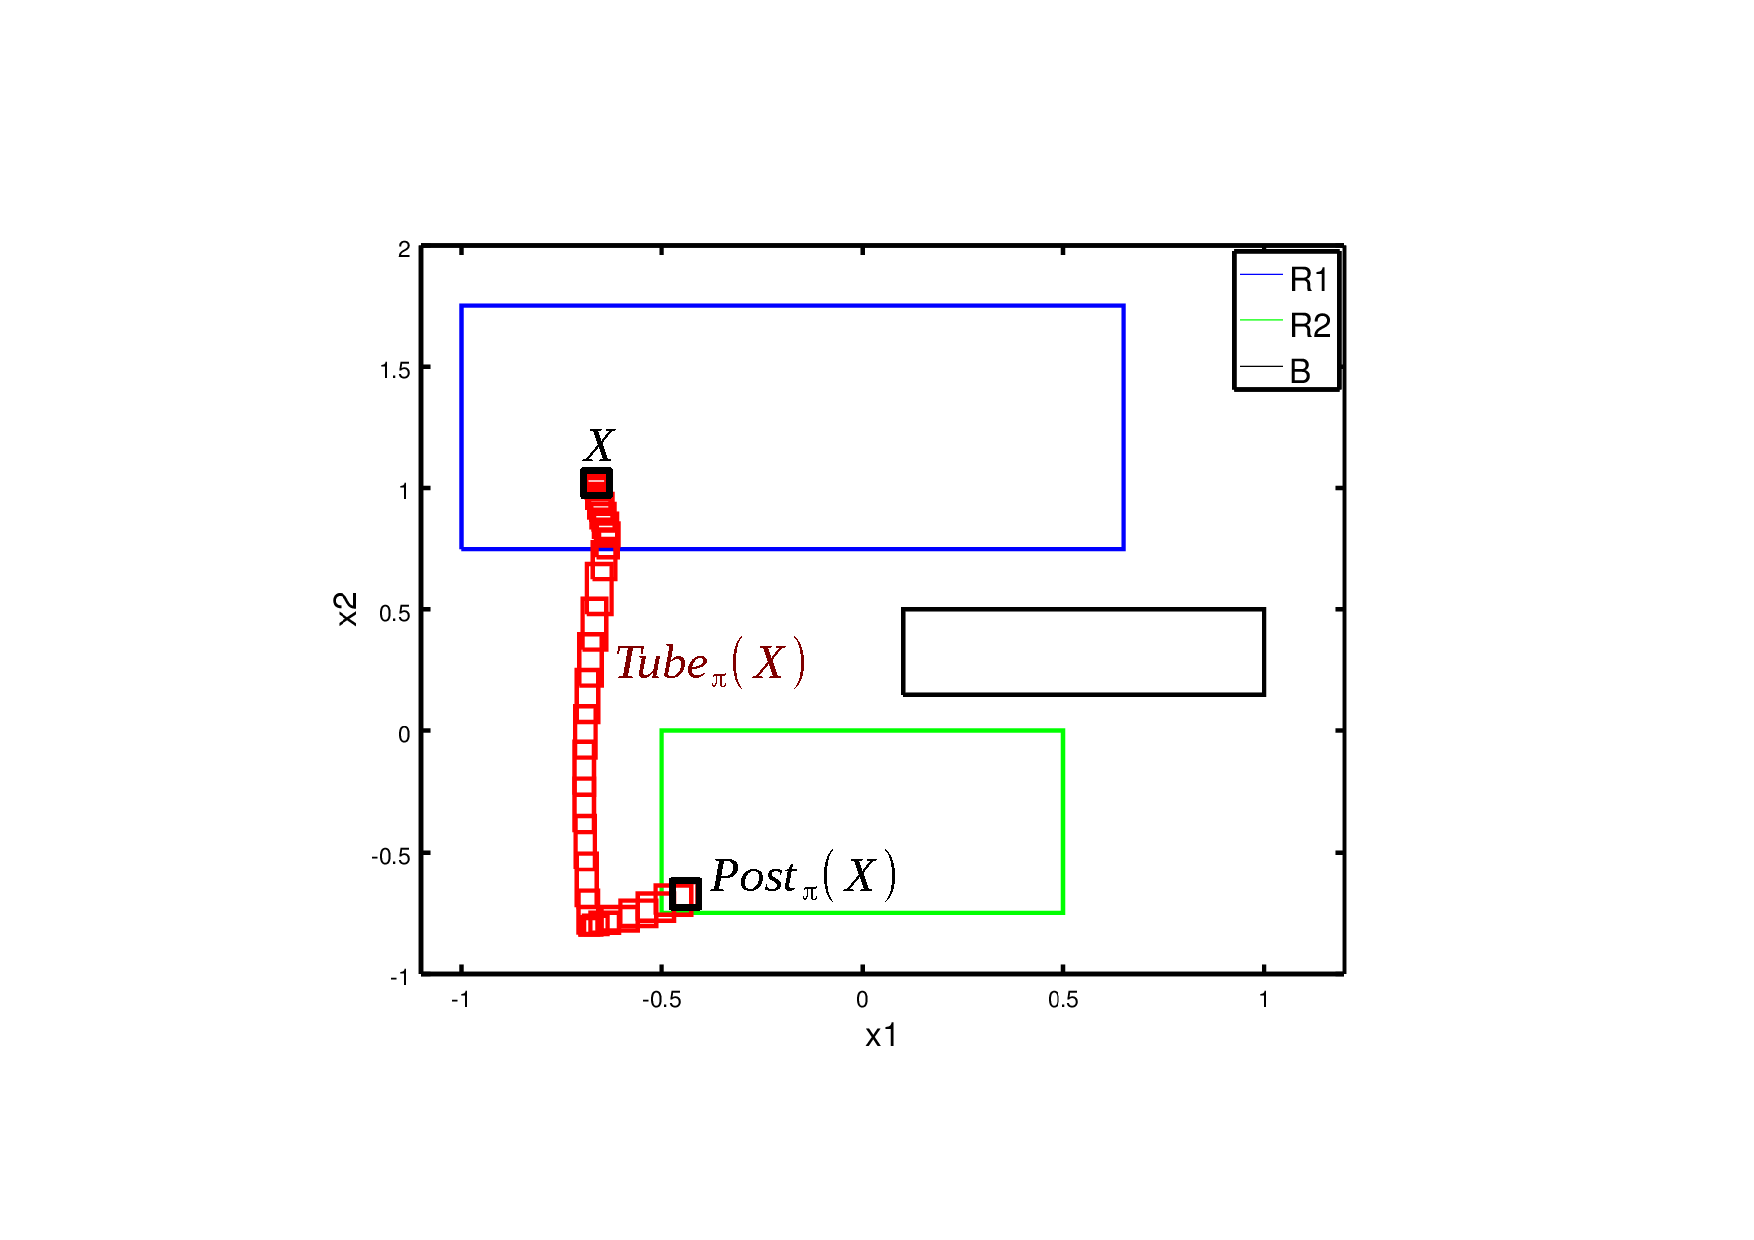
\includegraphics[trim = 4cm 3cm 4cm 4cm, clip,
width=0.5\textwidth]{tube.pdf}
 \caption{Functions $Post_{\pi}(X)$ and $Tube_{\pi}(X)$ for the
   initial box $X=[-0.69,-0.64] \times [1,1.06]$, with a pattern $\pi
   = (1,3,0)$.}
 \label{fig:post_illustration}
\end{figure}


\section{General principle}

We introduce a first basic procedure permitting to perform $(R,S)$-stability, and 
omit the perturbation in a first time.
Given a set $R$, let $\{W_i\}_{i \in I}$ be a family of 
sets such that $R \subseteq \bigcup_{i \in I} W_i \subseteq S$ as illustrated
in Figure \ref{fig:covering}.
If one can find, for each $W_i$ for $i \in I$, a pattern $\pi_i$
such that $Post_{\pi_i} (W_i) \subseteq R$, then we can induce 
an infinite-time switching rule permitting
to return infinitely often in $R$.


\begin{figure}[h]
\centering
 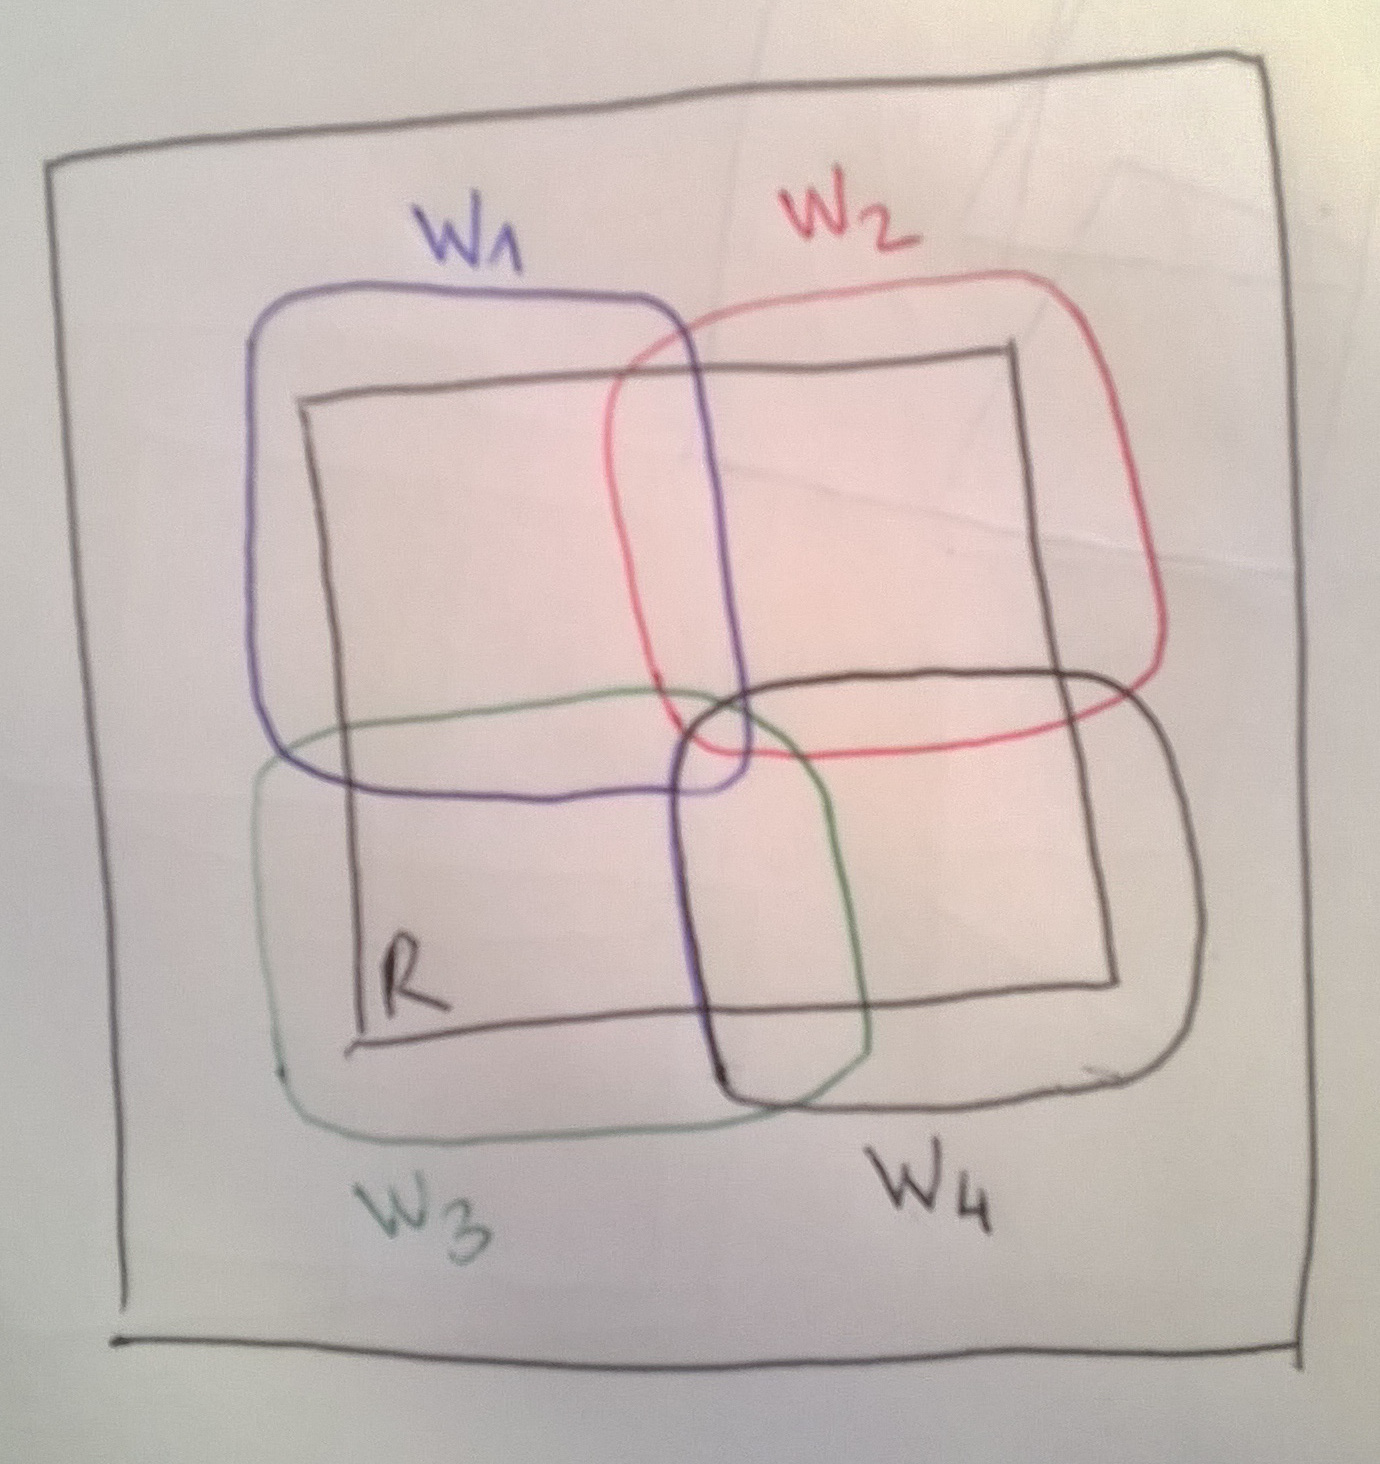
\includegraphics[scale=0.15]{covering.jpg}
 \label{fig:covering}
 \caption{A family of sets covering $R$.}
\end{figure}

\begin{theorem}
 Let $R \subseteq \R^n$, suppose we are given a
 switched system satisfying \eqref{eq:switched_system0}.
 A family of sets $\{W_i\}_{i \in I}$ associated to 
 patterns $\{\pi_i\}_{i \in I}$
 such that 
 \begin{itemize}
  \item $R \subseteq \bigcup_{i \in I} W_i \subseteq S$ 
  \item  for all $i \in I$, $Post_{\pi_i} (W_i) \subseteq R$
 \end{itemize}
 induces an infinite-time control ensuring recurrence in $R$. 
 \label{th:R-procedure}
\end{theorem}
\begin{proof}
 Let $x_0 \in R$, there exists $i_0 \in I$ such that $x_0 \in W_{i_0}$ since 
 $R \subseteq \bigcup_{i \in I} W_i$. Application of pattern 
 $\pi_{i_0}$ leads to a state $x_1 = \phi( \tau;0,x_0,\pi_{i_0})$
 also belonging to $R$ since $Post_{\pi_{i_0}}(W_{i_0}) \subseteq R$. State $x_1$
 thus belongs to $W_{i_1}$ for some $i_1 \in I$, and by recurrence, 
 one can obtain a sequence of points $x_0,x_1,\dots$ all belonging to 
 $R$. The induced trajectory thus returns infinitely often in $R$.
\end{proof}

A simple extension of this procedure, relying on the computation
of reachability tubes, allows to ensure safety in $S \subseteq \R^n$ as follows.

\begin{theorem}
 Let $R \subseteq \R^n$, $S \subseteq \R^n$, suppose we are given a
 switched system satisfying \eqref{eq:switched_system0}.
 A family of sets $\{W_i\}_{i \in I}$ associated to 
 patterns $\{\pi_i\}_{i \in I}$
 such that 
 \begin{itemize}
  \item $R \subseteq \bigcup_{i \in I} W_i \subseteq S$ 
  \item  for all $i \in I$, $Post_{\pi_i} (W_i) \subseteq R$
  \item  for all $i \in I$, $Tube_{\pi_i} (W_i) \subseteq S$
  \end{itemize}
 induces an infinite-time control ensuring recurrence in $R$ and safety in $S$. 
 \label{th:RS-procedure}
\end{theorem}
\begin{proof}
The recurrence in $R$ is proved with the same arguments as the proof 
of Theorem~\ref{th:R-procedure}. The safety in $S$ is ensured 
by the definition of $Tube_{\pi_i}(W_i)$, with permits 
to ensure that for all $x_0 \in R$, $i \in I$, $t \in k_i\tau$, where $k_i$
is the length of pattern $\pi_i$, we have
$\phi( t;0,x_0,\pi_{i}) \in S$.
\end{proof}

Having defined the principle of the procedure, we now present 
how controllers can be numerically computed 
using Theorem \ref{th:R-procedure} and \ref{th:RS-procedure}.
At this point, two main problems arise. The first is the construction
of a family $\{W_i\}_{i \in I}$ covering $R$, the second 
is ensuring that for all $i \in I$, $Post_{\pi_i} (W_i) \subseteq R$ and
$Tube_{\pi_i} (W_i) \subseteq S$.
The first problem can be solved using heuristics, but depends of 
the type of sets one uses, the second is actually impossible to ensure exactly, in the 
sense that solutions of ODEs are not known in general (particularly 
when the initial condition is a set).
Supposing that one can compute reachability sets and tubes, the procedure works
as follows in practice. First, we generate a coarse covering 
of $R$ (starting for example by considering the whole set $R$), 
we then try to compute patterns associated to each set of 
the covering. If this last step fails, we generate another finer tiling, performing 
for example a bisection of each dimension of $R$, and one now has to control
each bisected part of $R$.
This is a simple heuristics, but which works well in practice (as seen in the following Sections ???).
In the following, we use a uniform covering of $R$ with boxes and balls of $\R^n$. If each box or ball
is controlled, the problem is solved, otherwise, we use a finer covering. 
We address the problem of computing reachability sets and tubes in the following chapters.
% and introduce some hypotheses for this purpose.
We now present in details the possible heuristics and associated algorithms 
for control synthesis, supposing that one can compute 
the Post and Tube operators.

% We now introduce an algorithm for the recurrence only property in $R$,
% using zonotope transformations for linear systems,
% in association with a heuristics decomposing $R$. It showed to be very efficient 
% for practical use for linear systems, but unfortunately cannot guarantee safety between 
% time steps for continuous systems. However, if the system is formulated 
% in a discrete time form, formal guarantees of safety can be ensured.
% The algorithm is composed of two main functions, given in Algorithm \ref{algo:basic_decomposition}
% and \ref{algo:basic_findpat}.

% \begin{algorithm}
%   \centering
%   \begin{algorithmic}
%     \STATE{\textbf{Function:} $Decomposition(W,R,D,K)$}
%     \STATE{\begin{center}\line(1,0){150}\end{center}}
%     \STATE{\quad \textbf{Input:} A box $W$, a box $R$, a degree $D$ of bisection,
%       a length $K$ of input pattern}\STATE{\quad \textbf{Output:}$\langle\{(V_i,\pi_i)\}_{i},True\rangle$ or $\langle\_ ,False\rangle$}
%     \STATE{\begin{center}\line(1,0){150}\end{center}}
%     \STATE{ $(\pi,b) := Find\_Pattern(W,R,K)$}
%     \IF{$b=True$}{
%       \STATE{\textbf{return} $\langle\{(W,Pat)\},True\rangle$}
%     }
%     \ELSE
%     \IF{$D = 0$} \RETURN{$\langle \_,False\rangle$} \ELSE
%     \STATE{Divide equally $W$ into $(W_1, W_{2})$ \FOR{$i=1,2$}\STATE{\small{$(\Delta_i,b_i)$ := $Decomposition(W_i,R,D - 1,K)$}}\ENDFOR
%       \RETURN $(\bigcup_{i=1,2} \Delta_i,\bigwedge_{i=1,2} b_i)$ } \ENDIF
%     \ENDIF
%   \end{algorithmic}
%   \caption{Algorithmic form of Function $Decomposition$.}
%   \label{algo:basic_decomposition}
% \end{algorithm}
% 
% 
% 
% \begin{algorithm}[t]
%   \centering
%   \begin{algorithmic}
%     \STATE{\textbf{Function:} $Find\_Pattern(W,R,K)$}
%     \STATE{\begin{center}\line(1,0){150}\end{center}}
%     \STATE{\quad \textbf{Input:}A box $W$, a box $R$, a length $K$ of input pattern}
%     \STATE{\quad \textbf{Output:}$\langle \pi,True\rangle$ or $\langle\_, False\rangle$}
%     \STATE{\begin{center}\line(1,0){150}\end{center}}
%     \FOR{$i=1\dots K$} \STATE{$\Pi :=$ set of input patterns of length $i$}
%     \WHILE{$\Pi$ is non empty} \STATE{Select $\pi$ in $\Pi$}
%     \STATE{$\Pi:= \Pi\setminus  \{\pi\}$}
%     \IF{$Post_{\pi}(W) \subseteq R$}{\RETURN{$\langle \pi,True\rangle$}} \ENDIF
%     \ENDWHILE
%     \ENDFOR
%     \RETURN{$\langle \_,False \rangle$}
%   \end{algorithmic}
%   \caption{Algorithmic form of Function $Find\_Pattern$.}
%   \label{algo:basic_findpat}
% \end{algorithm}


\subsection{The state-space bisection algorithm}
\label{sec:minimator}

% \subsubsection{Principle of the algorithm}

We describe the algorithm solving the control synthesis problem for
nonlinear switched systems (see Problem~\ref{prob:nl_control},
Section~\ref{sec:intro_detailed}). Given the input boxes $R$, $S$, $B$, and
given two positive integers $K$ and $D$, the algorithm provides, when
it succeeds, a decomposition $\Delta$ of $R$ of the form $\{ V_i,
\pi_i \}_{i \in I}$, with the properties:
\begin{itemize}
\item $\bigcup_{i \in I} V_i = R$,
\item $\forall i \in I, \ Post_{\pi_i}(V_i) \subseteq R$,
\item $\forall i \in I, \ Tube_{\pi_i}(V_i) \subseteq S$,
\item $\forall i \in I, \ Tube_{\pi_i}(V_i) \bigcap B = \emptyset$.
\end{itemize}

The sub-boxes $\{ V_i \}_{i \in I}$ are obtained by repeated
bisection.  At first, function $Decomposition$ calls sub-function
$Find\_Pattern$ which looks for a pattern $\pi$ of length at most $K$
such that $Post_{\pi}(R) \subseteq R$, $Tube_{\pi}(R) \subseteq S$ and
$Tube_{\pi}(R) \bigcap B = \emptyset$.  If such a pattern $\pi$ is
found, then a uniform control over $R$ is found (see
Figure~\ref{fig:scheme}(a)). Otherwise, $R$ is divided into two
sub-boxes $V_1$, $V_{2}$, by bisecting $R$ w.r.t. its longest
dimension. Patterns are then searched to control these sub-boxes (see
Figure~\ref{fig:scheme}(b)). If for each $V_i$, function
$Find\_Pattern$ manages to get a pattern $\pi_i$ of length at most $K$
verifying $Post_{\pi_i}(V_i) \subseteq R$, $Tube_{\pi_i}(V_i)
\subseteq S$ and $Tube_{\pi_i}(V_i) \bigcap B = \emptyset$, then it is
a success and algorithm stops.  If, for some $V_j$, no such pattern is
found, the procedure is recursively applied to $V_j$.  It ends with
success when every sub-box of $R$ has a pattern verifying the latter
conditions, or fails when the maximal degree of decomposition $D$ is
reached.  The algorithmic form of functions $Decomposition$ and
$Find\_Pattern$ are given in Algorithm~\ref{algo:decomposition} and
Algorithm~\ref{algo:findpattern} respectively. Note that a special form
of Algorithm~\ref{algo:findpattern} for linear ODEs can be found
in~\cite{fribourg2014finite}.

\begin{figure}[ht]
 \centering
 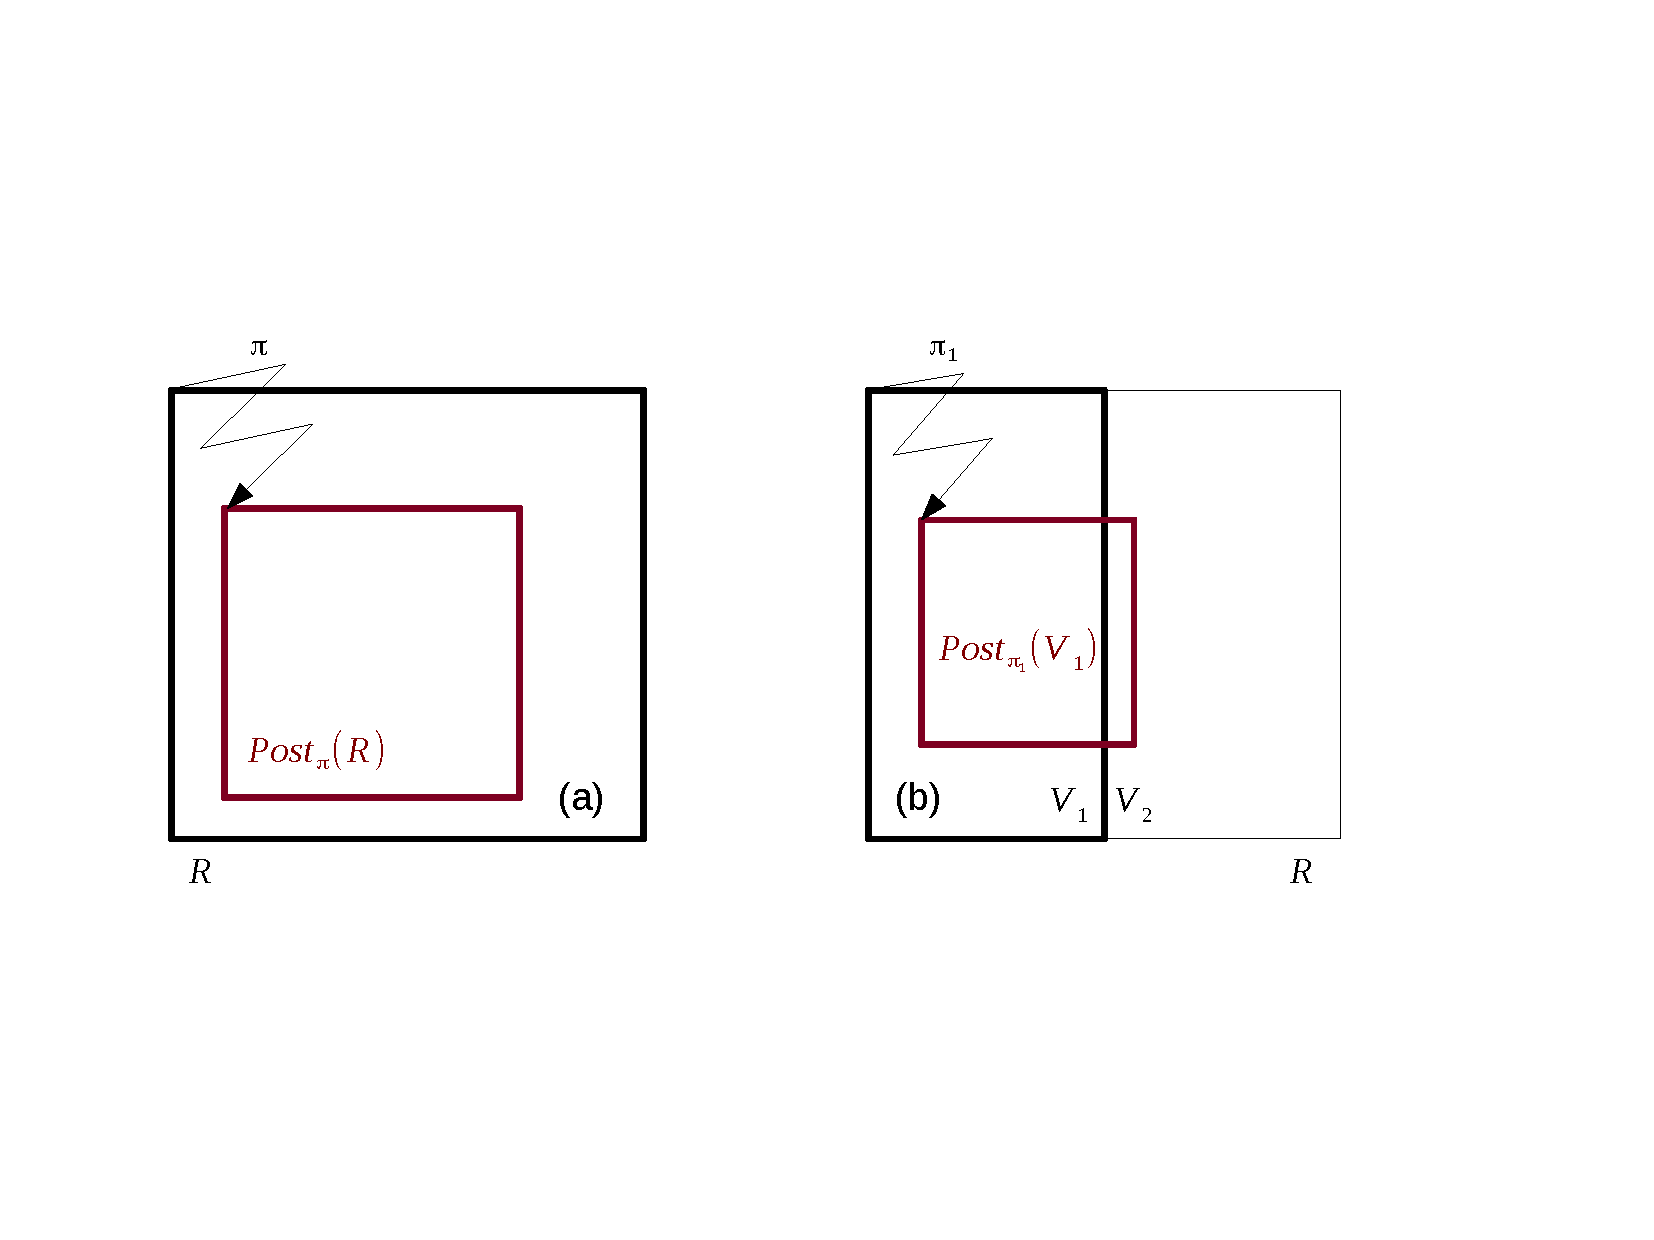
\includegraphics[%trim = 2cm 6cm 4cm 5.5cm, clip,
 width=0.6\textwidth]{bisect.pdf}
 \caption{Principle of the bisection method.}
 \label{fig:scheme}
\end{figure}


\begin{algorithm}
  \centering
  \begin{algorithmic}
    \STATE{\textbf{Function:} $Decomposition(W,R,S,B,D,K)$}
    \STATE{\begin{center}\line(1,0){150}\end{center}}
    \STATE{\quad \textbf{Input:} A box $W$, a box $R$, a box $S$, a box $B$, a degree $D$ of bisection,
      a length $K$ of input pattern}\STATE{\quad \textbf{Output:}$\langle\{(V_i,\pi_i)\}_{i},True\rangle$ or $\langle\_ ,False\rangle$}
    \STATE{\begin{center}\line(1,0){150}\end{center}}
    \STATE{ $(\pi,b) := Find\_Pattern(W,R,S,B,K)$}
    \IF{$b=True$}{
      \STATE{\textbf{return} $\langle\{(W,Pat)\},True\rangle$}
    }
    \ELSE
    \IF{$D = 0$} \RETURN{$\langle \_,False\rangle$} \ELSE
    \STATE{Divide equally $W$ into $(W_1, W_{2})$ \FOR{$i=1,2$}\STATE{\small{$(\Delta_i,b_i)$ := $Decomposition(W_i,R,S,B,D - 1,K)$}}\ENDFOR
      \RETURN $(\bigcup_{i=1,2} \Delta_i,\bigwedge_{i=1,2} b_i)$ } \ENDIF
    \ENDIF
  \end{algorithmic}
  \caption{Algorithmic form of Function $Decomposition$.}
  \label{algo:decomposition}
\end{algorithm}


Our control synthesis method being well defined, we introduce the main
result of this section, stated as follows:
 \begin{proposition}
   Algorithm~\ref{algo:decomposition} with input
   $(R,R,S,B,D,K)$ returns, when it successfully terminates, a
   decomposition $\{ V_i,\pi_i \}_{i \in I}$ of~$R$ which solves
   Problem~\ref{prob:nl_control}.
 \end{proposition}
%
 \begin{proof}
   Let $x_0 = x(t_0=0)$ be an initial condition belonging to~$R$. If
   the decomposition has terminated successfully, we have $\bigcup_{i
     \in I} V_i = R$, and $x_0$ thus belongs to $V_{i_0}$ for some
   $i_0\in I$.  We can thus apply the pattern $\pi_{i_0}$ associated
   to $V_{i_0}$. Let us denote by $k_0$ the length of $\pi_{i_0}$. We
   have:
   \begin{itemize}
   \item $\phi_{\pi_{i_0}}(k_0\tau;0,x_0,d) \in R$
   \item $\forall t \in [0, k_0\tau], \quad
     \phi_{\pi_{i_0}}(t;0,x_0,d) \in S$
   \item $\forall t \in [0, k_0\tau], \quad
     \phi_{\pi_{i_0}}(t;0,x_0,d) \notin B$
   \end{itemize}
   Let $x_1 = \phi_{\pi_{i_0}}(k_0\tau;0,x_0,d) \in R$ be the
   state reached after application of $\pi_{i_0}$ and let $t_1 = k_0
   \tau$.  State $x_1$ belongs to $R$, it thus belongs to $V_{i_1}$
   for some $i_1 \in I$, and we can apply the associated pattern
   $\pi_{i_1}$ of length $k_1$, leading to:
   \begin{itemize}
   \item $\phi_{\pi_{i_1}}(t_1 + k_1\tau;t_1,x_1,d) \in R$
   \item $\forall t \in [t_1, t_1 + k_1\tau], \quad
     \phi_{\pi_{i_1}}(t;t_1,x_1,d) \in S$
   \item $\forall t \in [t_1, t_1 + k_1\tau], \quad
     \phi_{\pi_{i_1}}(t;t_1,x_1,d) \notin B$
   \end{itemize}
   We can then iterate this procedure from the new state
   \begin{displaymath}
     x_2 =
     \phi_{\pi_{i_1}}(t_1 + k_1\tau;t_1,x_1,d) \in R.
   \end{displaymath}
   This can be repeated infinitely, yielding a sequence of points
   belonging to $R$ $x_0,x_1,x_2,\dots$ attained at times
   $t_0,t_1,t_2,\dots$, when the patterns
   $\pi_{i_0},\pi_{i_1},\pi_{i_2},\dots$ are applied.

   We furthermore have that all the trajectories stay in $S$ and never
   cross $B$:
   \begin{displaymath}
     \forall t \in \mathbb{R}^+, \exists k \geq 0, \ t \in
     \lbrack t_k , t_{k+1} \rbrack
   \end{displaymath}
   and
   \begin{displaymath}
     \forall t \in \lbrack t_k ,
     t_{k+1} \rbrack,\ \phi_{\pi_{i_k}} ( t; t_k, x_k, d) \in S,\
     \phi_{\pi_{i_k}} (t;t_k, x_k, d) \notin B .
   \end{displaymath}
   The trajectories thus return infinitely often in $R$, while always
   staying in $S$ and never crossing $B$.
\end{proof}

 \begin{remark}
   Note that it is possible to perform reachability from a set $R_1$
   to another set $R_2$ by computing $Decomposition(R_1,R_2,S,B,D,K)$.
   The set $R_1$ is thus decomposed with the objective to send its
   sub-boxes into $R_2$, \textit{i.e.}, for a sub-box $V$ of $R_1$,
   patterns $\pi$ are searched with the objective $Post_{\pi}(V)
   \subseteq R_2$ (see Example~\ref{ex2}).
 \end{remark}

\begin{algorithm}[t]
  \centering
  \begin{algorithmic}
    \STATE{\textbf{Function:} $Find\_Pattern(W,R,S,B,K)$}
    \STATE{\begin{center}\line(1,0){150}\end{center}}
    \STATE{\quad \textbf{Input:}A box $W$, a box $R$, a box $S$, a box $B$, a length $K$ of input pattern}
    \STATE{\quad \textbf{Output:}$\langle \pi,True\rangle$ or $\langle\_, False\rangle$}
    \STATE{\begin{center}\line(1,0){150}\end{center}}
    \FOR{$i=1\dots K$} \STATE{$\Pi :=$ set of input patterns of length $i$}
    \WHILE{$\Pi$ is non empty} \STATE{Select $\pi$ in $\Pi$}
    \STATE{$\Pi:= \Pi\setminus  \{\pi\}$}
    \IF{$Post_{\pi}(W) \subseteq R$ \AND $Tube_{\pi}(W) \subseteq S$ \AND $Tube_{\pi}(W) \bigcap B = \emptyset$ }{\RETURN{$\langle \pi,True\rangle$}} \ENDIF
    \ENDWHILE
    \ENDFOR
    \RETURN{$\langle \_,False \rangle$}
  \end{algorithmic}
  \caption{Algorithmic form of Function $Find\_Pattern$.}
  \label{algo:findpattern}
\end{algorithm}


In Algorithm \ref{algo:decomposition} and \ref{algo:findpattern}, 
we use a bisection of uncontrolled tiles into two parts (by bisecting the greatest 
dimension). But another possible heuristics is to divide 
uncontrolled parts into $2^n$ parts, by bisecting each dimension. 
This leads to a faster growing of the number of tiles to be controlled, but 
can sometimes lead to lower computation times, when the system requires a fine tiling. 
The two possible heuristics are schemed in Figure \ref{fig:heuristics}. 

\begin{figure}
\centering
 \begin{tabular}{cc}
  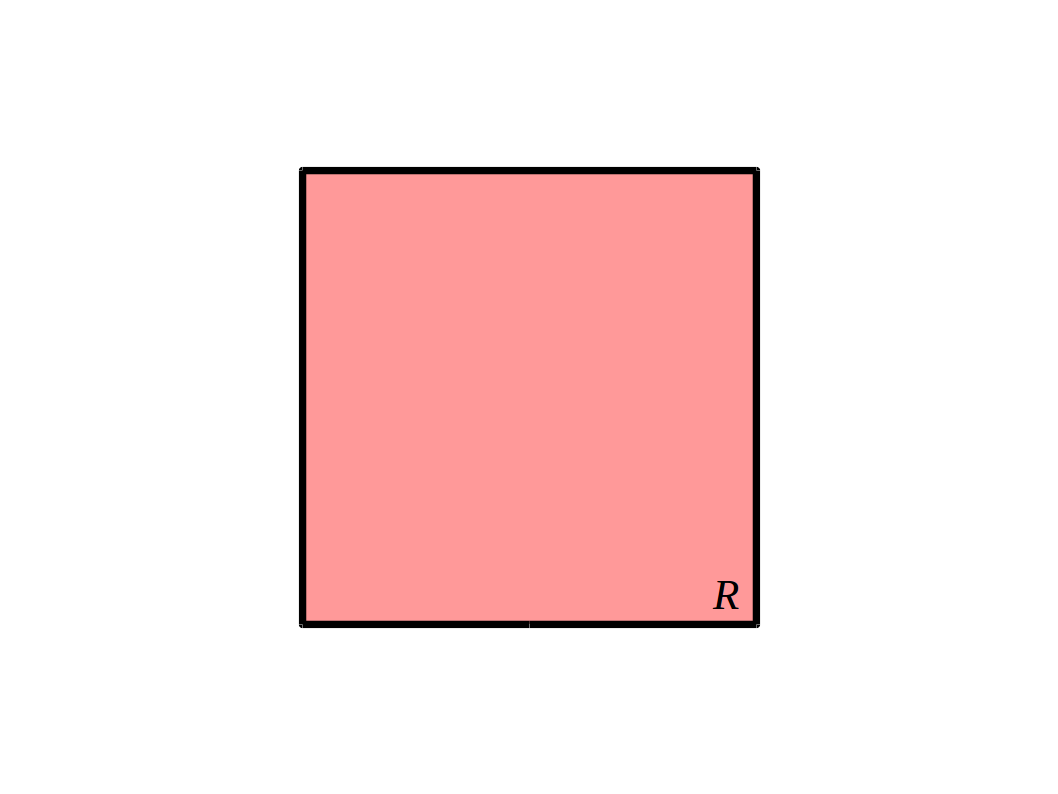
\includegraphics[width=0.4\textwidth]{tiling_R_heuristics102.png} &   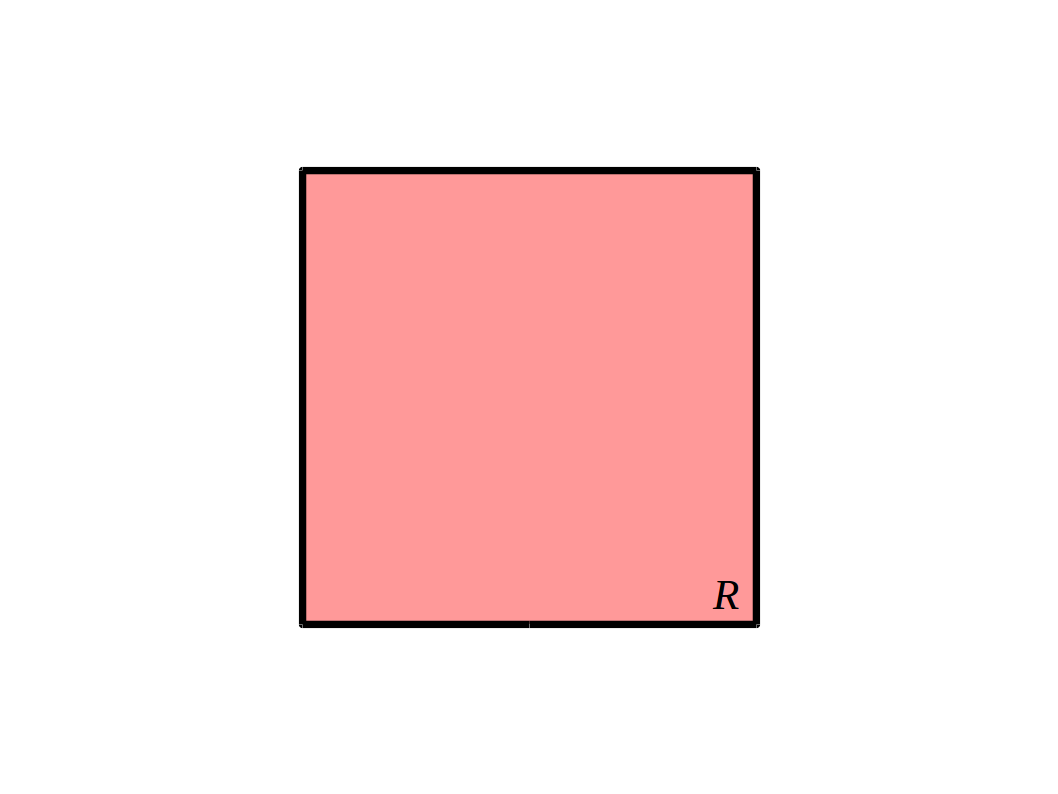
\includegraphics[width=0.4\textwidth]{tiling_R_heuristics102.png} \\
  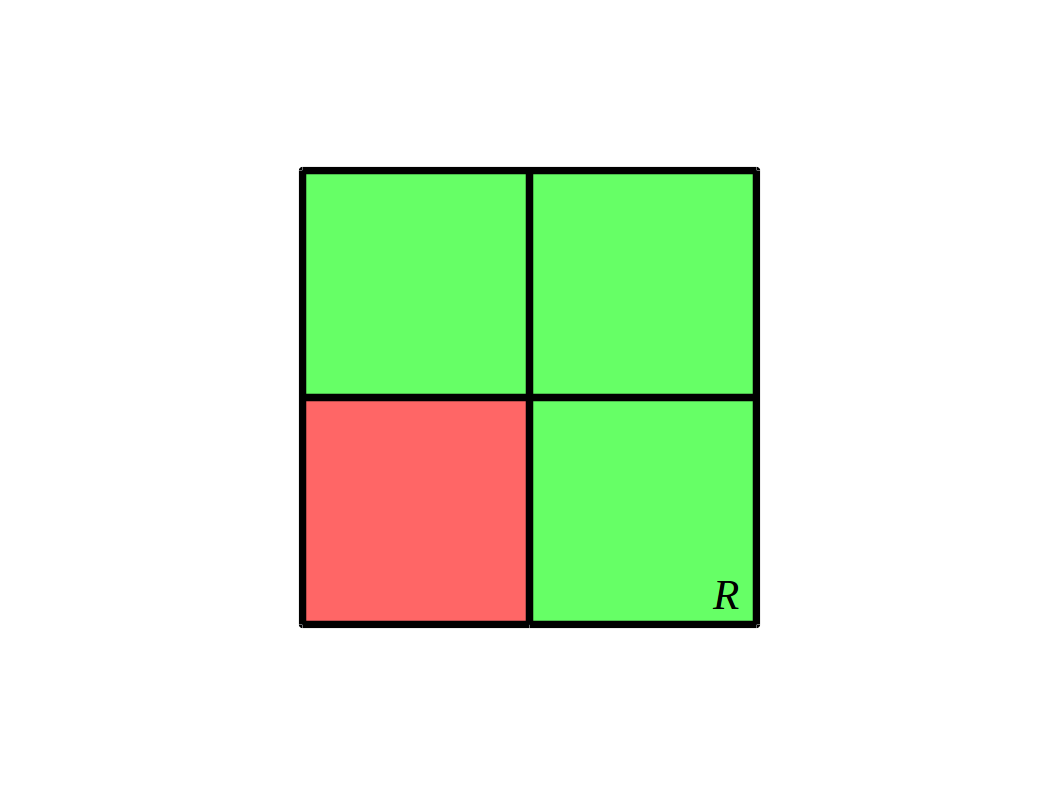
\includegraphics[width=0.4\textwidth]{tiling_R_heuristics112.png} &   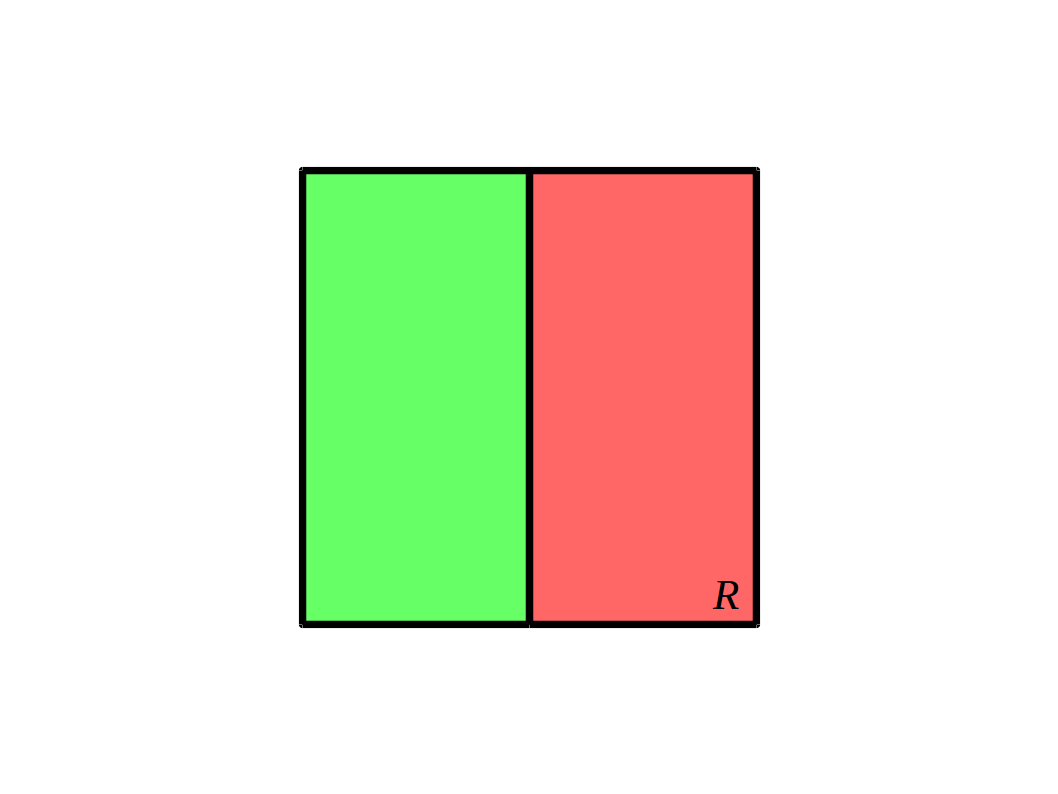
\includegraphics[width=0.4\textwidth]{tiling_R_heuristics212.png} \\  
  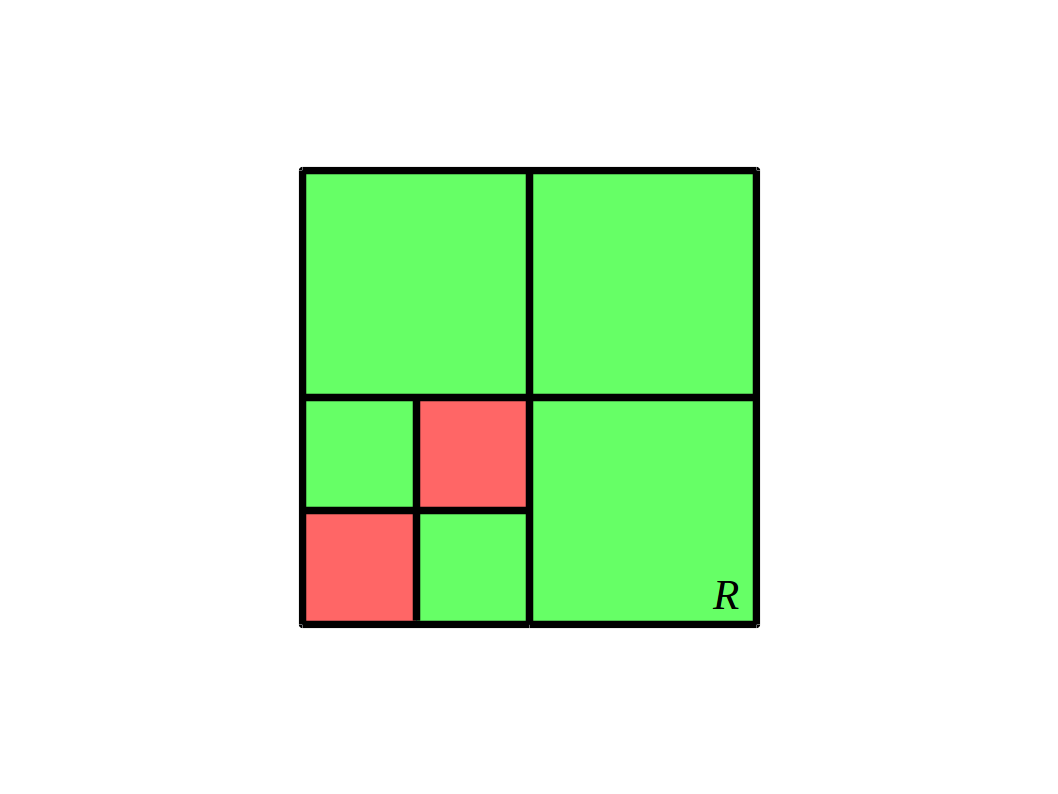
\includegraphics[width=0.4\textwidth]{tiling_R_heuristics122.png} &   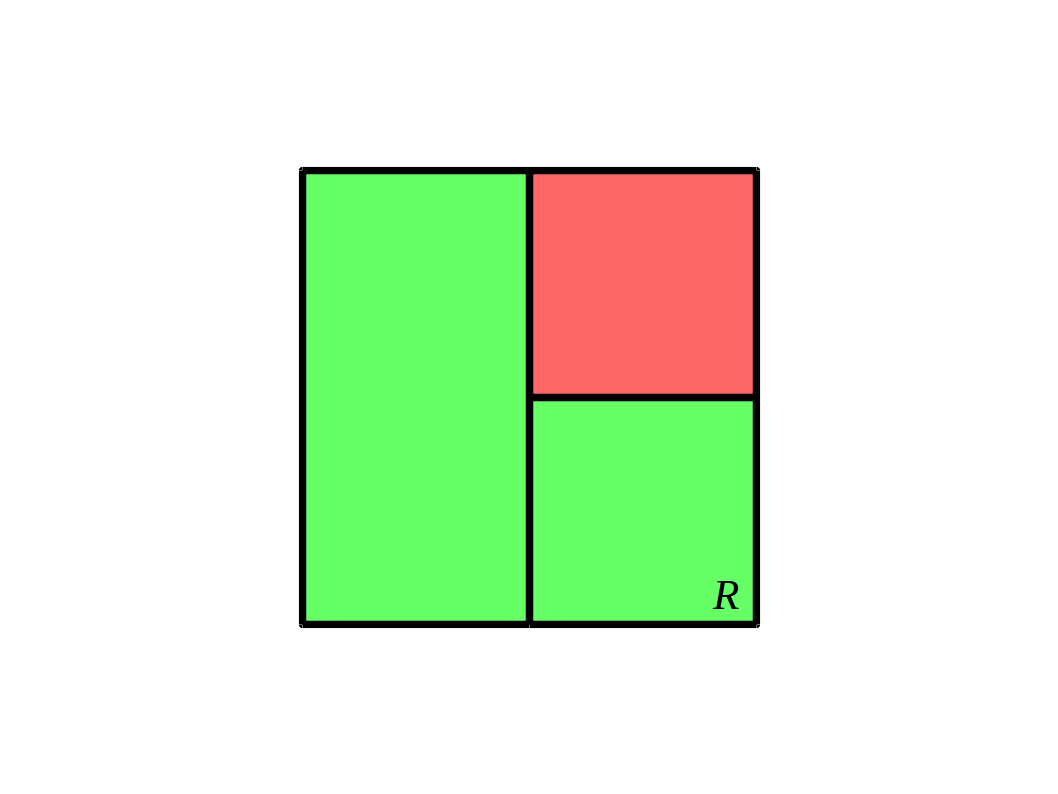
\includegraphics[width=0.4\textwidth]{tiling_R_heuristics222.png} \\  
  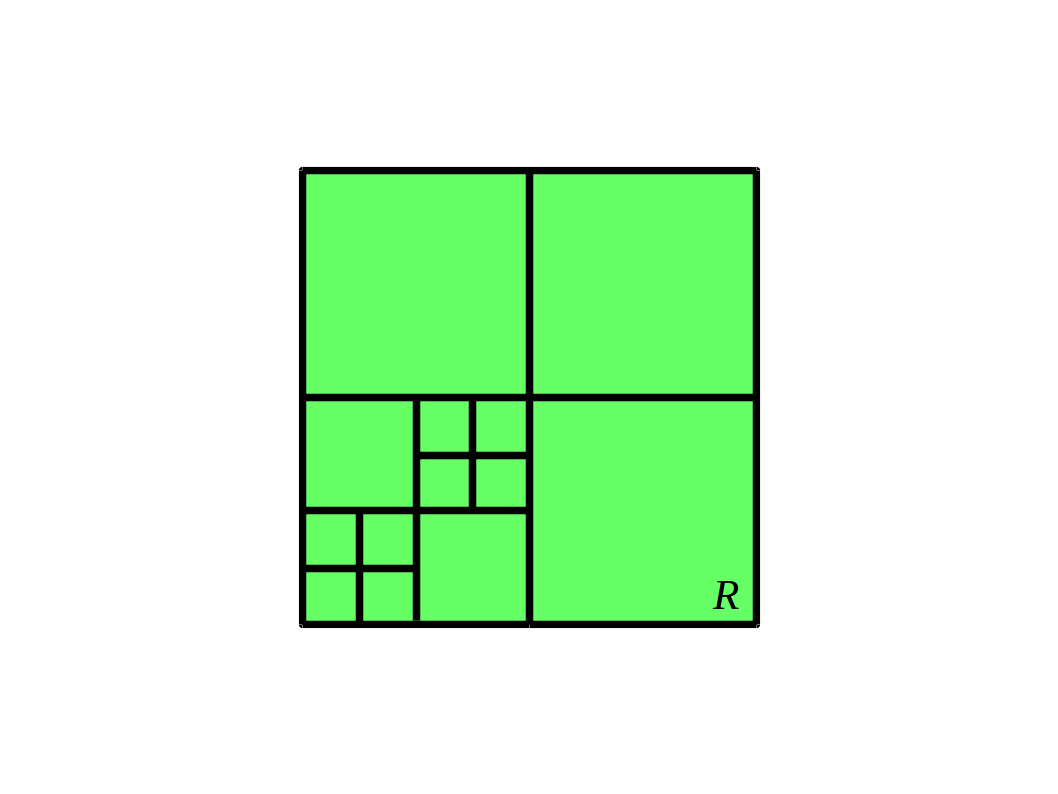
\includegraphics[width=0.4\textwidth]{tiling_R_heuristics132.png} &   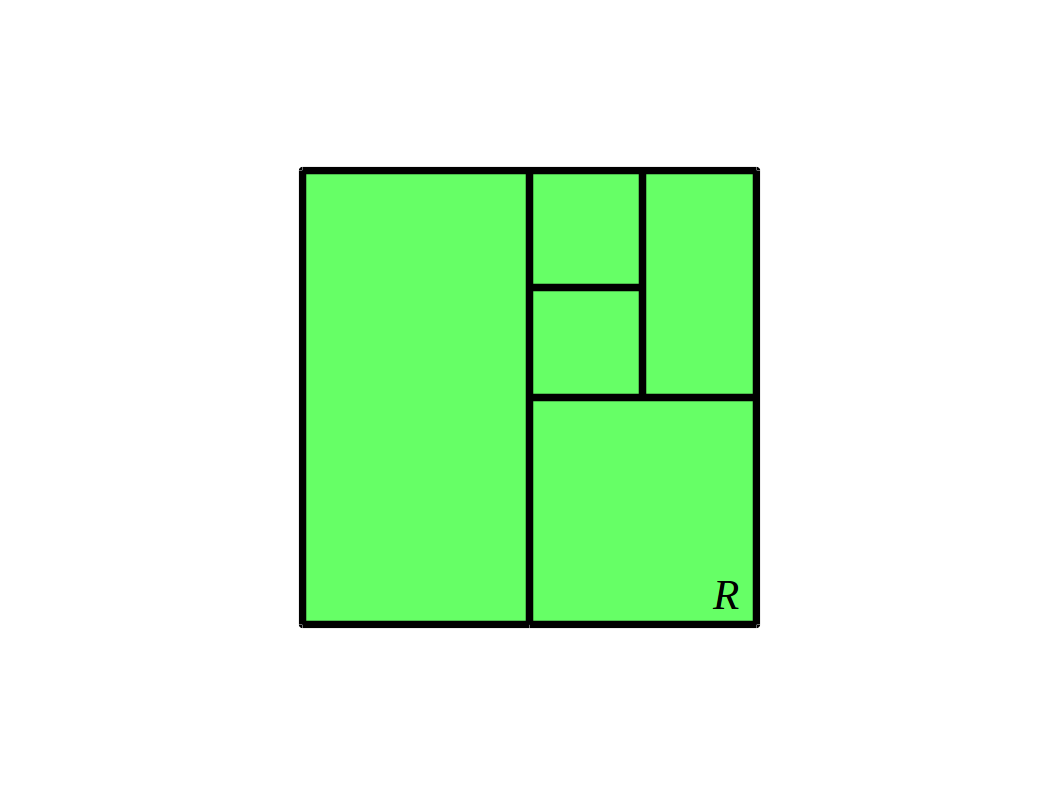
\includegraphics[width=0.4\textwidth]{tiling_R_heuristics242.png} \\  
  \end{tabular}
 \caption{Scheme of the two possible heuristics: green 
tiles have been controlled (associated to a pattern), and red tiles have yet to be controlled and
bisected. Left: bisection of all the dimensions; right: bisection of the largest dimension}
\label{fig:heuristics}
\end{figure}


  \subsection{A covering of balls}

  So far, we used boxes of $\R^n$ to represent sets of states.
  Balls of $\R^n$ are actually another useful way of representing it, since we provide 
  an efficient way of performing reachability analysis with such sets (see Chapter \ref{chap:1}).
  A covering of $R$ can be performed as schemed in Figure \ref{fig:tilingball}.
  Let $\delta$ be a radius, each set $W_i = B(\tilde x_i, \delta)$ has to be controlled, otherwise,
  a fined covering (using more balls) should be used.
  Actually, the same heuristics as boxes could be used, since these balls 
  can be built as circumscribed balls of the boxes.
  
  
  
  \begin{figure}
  \centering
   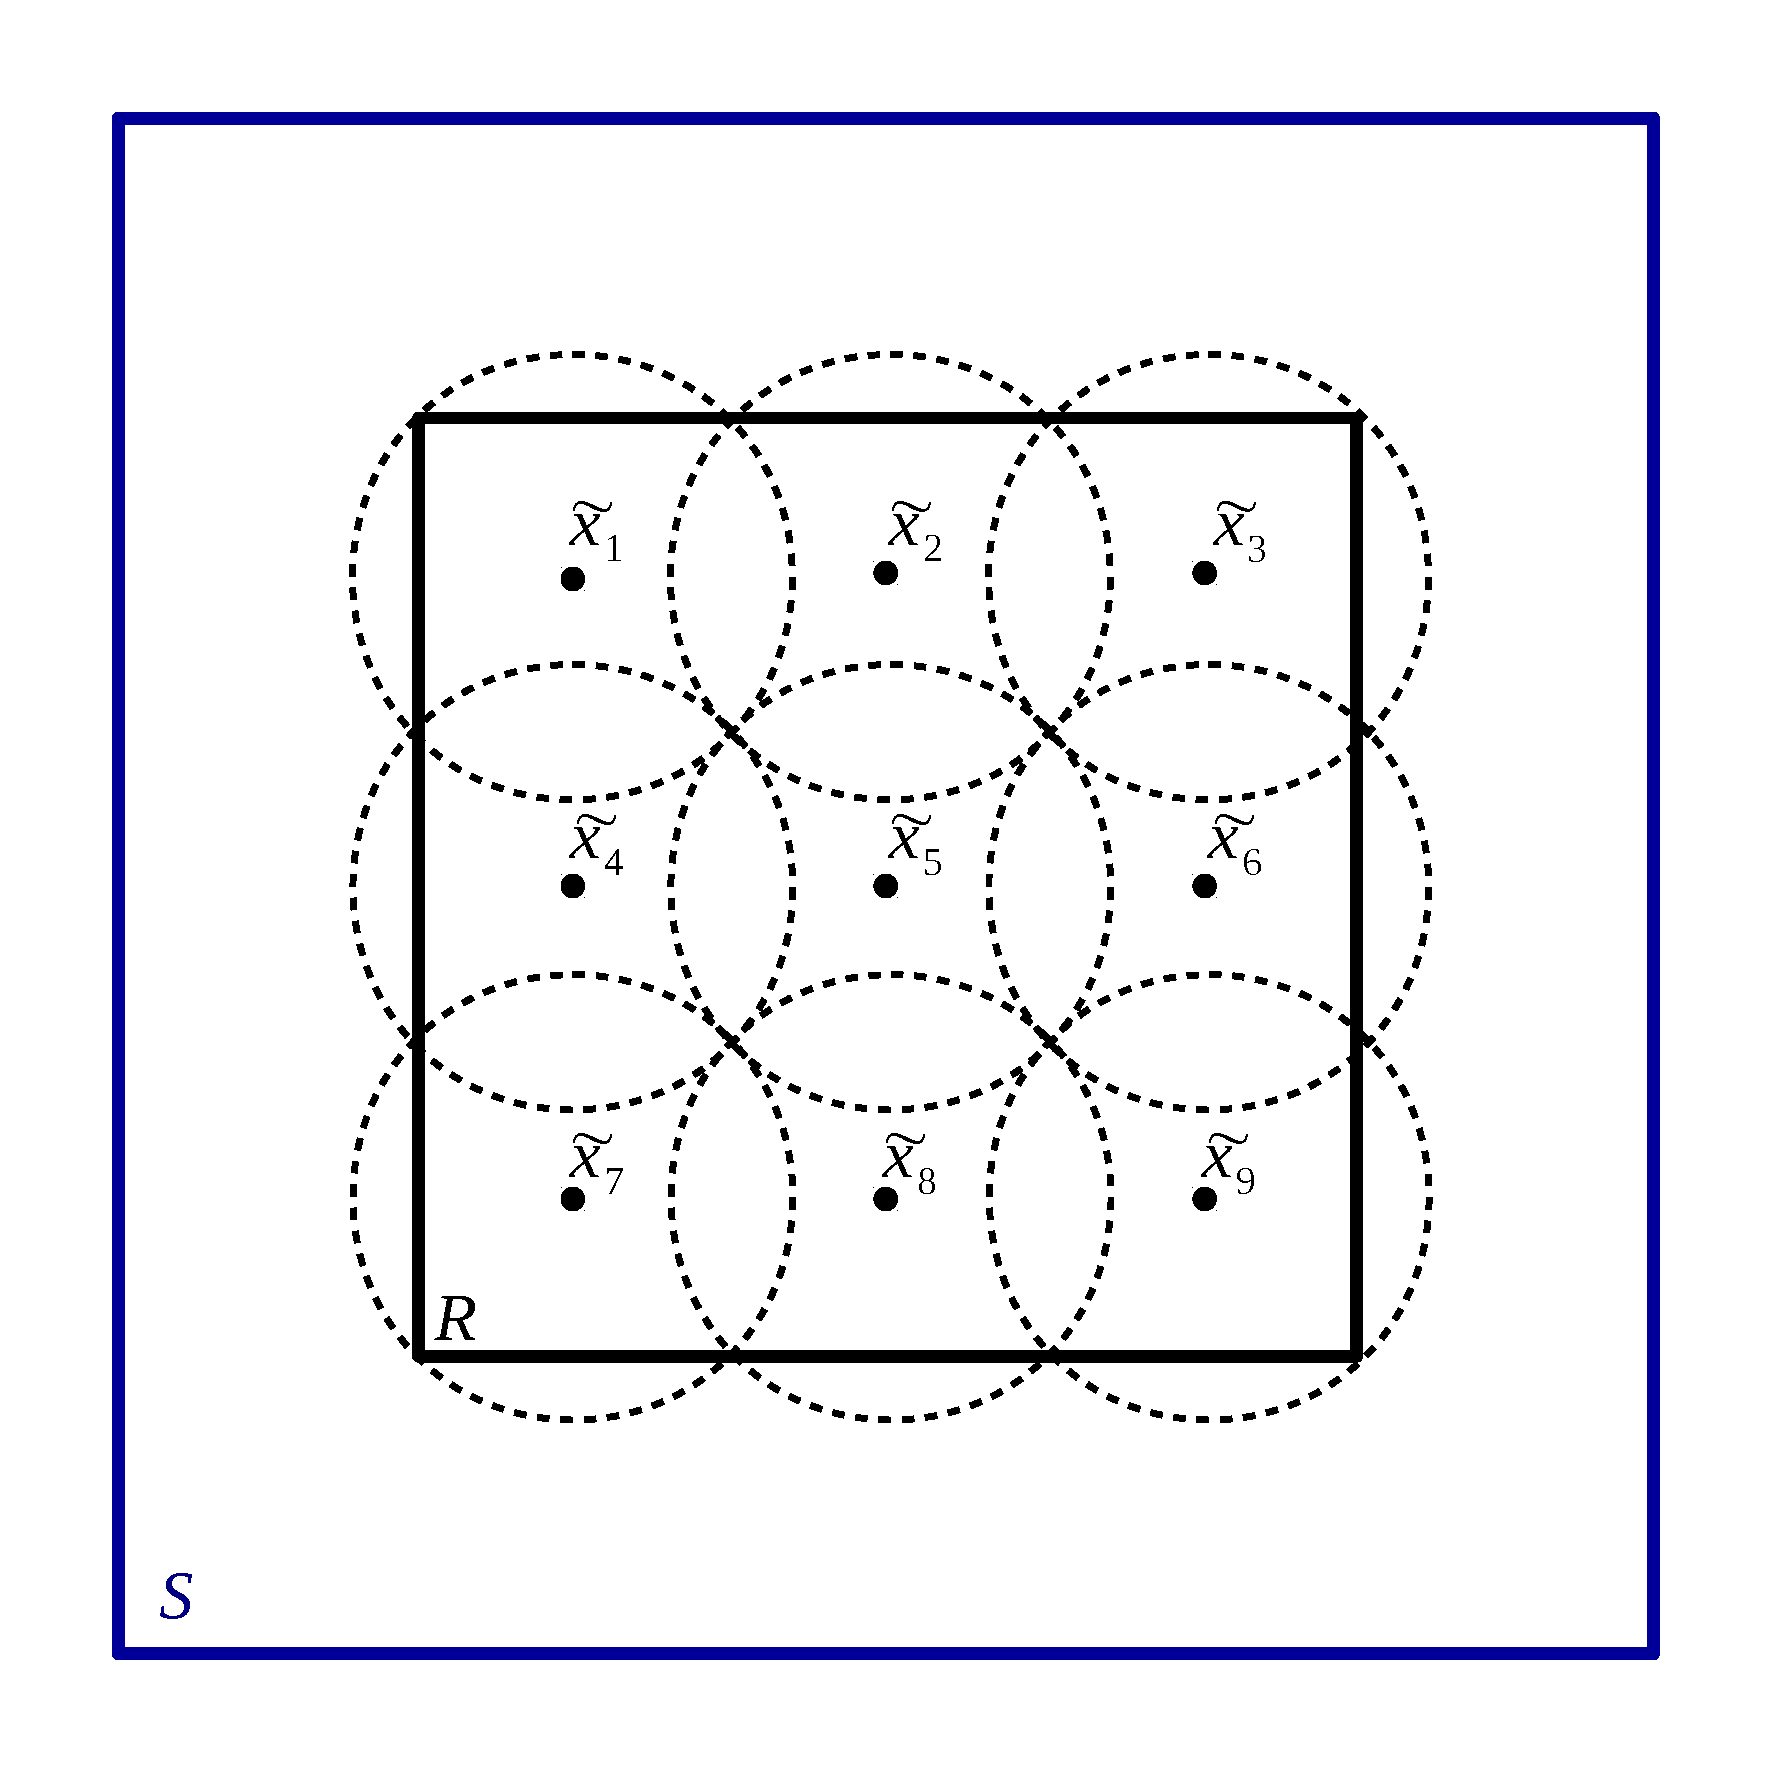
\includegraphics[width=0.5\textwidth]{tilingball2.pdf}
   \caption{Scheme of a covering of $R \subset \R^2$ with balls.}
   \label{fig:tilingball}
  \end{figure}

  
 \subsection{Improving the research of patterns}
%
 We propose in this section an improvement of the function
 $Find\_Pattern$ given in~\cite{NL_minimator,fribourg2014finite},
 which is a naive testing of all the patterns of growing length (up to
 $K$).


 \begin{algorithm}[t]
   \centering
   \begin{algorithmic}
     \STATE{\textbf{Function:} $Find\_Pattern2(W,R,S,B,K)$}
     \STATE{\begin{center}\line(1,0){150}\end{center}}
     \STATE{\quad \textbf{Input:}A box $W$, a box $R$, a box $S$, a box $B$, a length $K$ of input pattern}
     \STATE{\quad \textbf{Output:}$\langle \pi,True\rangle$ or $\langle\_, False\rangle$}
     \STATE{\begin{center}\line(1,0){150}\end{center}}

     \STATE{$\mathcal{S} = \{  \emptyset \}$}
     \STATE{$\mathcal{L} = \{ \left(W,W, \emptyset \right) \}$}
     \WHILE{$\mathcal{L} \neq \emptyset$} \STATE{$e_{\text{current}}$ = takeHead($\mathcal{L}$)}

 \FOR{$i \in U$}
    \IF{$Post_{i}(e_{\text{current}}.Y_{\text{current}}) \subseteq R$ \AND $Tube_{i}(e_{\text{current}}.{Y_{\text{current}}}) \bigcap B = \emptyset$ \AND $Tube_{i}(e_{\text{current}}.Y_{\text{current}}) \subseteq S$} \STATE{$\text{putTail}(\mathcal{S},e_{\text{current}}.\Pi + i)$ {\color{blue} /* or also ``{\bf return} $\langle e_{\text{current}}.\Pi + i,True \rangle$'' */ } }
  \ELSE{ \IF{$Tube_{i}(e_{\text{current}}.{Y_{\text{current}}}) \bigcap B \neq \emptyset$ \OR
      $Tube_{i}(e_{\text{current}}.{Y_{\text{current}}}) \nsubseteq S$} \STATE{ discard $e_{\text{current}}$ } \ENDIF}
    \ELSE{ \IF{$Tube_{i}(e_{\text{current}}.{Y_{\text{current}}}) \bigcap B = \emptyset$ \AND $Tube_{i}(e_{\text{current}}.Y_{\text{current}}) \subseteq S$}
      \STATE{\IF{$\text{Length}(\Pi)+1 < K$} \STATE{$\text{putTail}(\mathcal{L},\left(e_{\text{current}}.Y_{\text{init}}, Post_i(e_{\text{current}}.Y_{\text{current}}),e_{\text{current}}.\Pi + i \right))$ }   \ENDIF} \ENDIF}

    \ENDIF
  \ENDFOR
 \ENDWHILE

 \RETURN{$\langle \_,False \rangle$ if no solution is found, or $\langle \pi,True\rangle$, $\pi$ being
 any pattern validated in $Solution$.}
 \end{algorithmic}
\caption{Algorithmic form of Function $Find\_Pattern2$.}
\label{algo:findpattern2}
\end{algorithm}


 The improved function, denoted here by $Find\_Pattern2$, exploits
 heuristics to prune the search tree of patterns. We present it
 with boxes of $\R^n$, but can also be used with balls. The algorithmic form
 of $Find\_Pattern2$ is given in Algorithm~\ref{algo:findpattern2}.  It
 relies on a new data structure consisting of a list of triplets
 containing:
 \begin{itemize}
 \item An initial box $V \subset \mathbb{R}^n$,
  \item A {\em current} box $Post_{\pi}(V)$, image of $V$ by the pattern $\pi$,
  \item The associated pattern $\pi$.
 \end{itemize}
 For any element $e$ of a list of this type, we denote by $e.Y_{\text{init}}$
 the initial box, $e.Y_{\text{current}}$ the {\em current} box, and by
 $e.\Pi$ the associated pattern.  We denote by $e_{\text{current}} =
 takeHead(\mathcal{L})$ the element on top of a list $\mathcal L$
 (this element is removed from list $\mathcal L$).  The function
 $putTail(\cdot,\mathcal{L})$ adds an element at the end of the list
 $\mathcal L$.

 Let us suppose one wants to control a box $X \subseteq R$.  The list
 $\mathcal{L}$ of Algorithm~\ref{algo:findpattern2} is used to store the
 intermediate computations leading to possible solutions (patterns
 sending $X$ in $R$ while never crossing $B$ or $\mathbb{R}^n
 \setminus S$). It is initialized as $\mathcal{L} = \{ \left(X,X,
   \emptyset \right) \}$.  First, a testing of all the control modes
 is performed (a set simulation starting from $X$ during time $\tau$
 is computed for all the modes in $U$).  The first level of branches
 is thus tested exhaustively. If a branch leads to crossing $B$ or
 $\mathbb{R}^n \setminus S$, the branch is cut. Indeed, no following
 branch can be accepted if a previous one crosses $B$.  It is one of
 the improvements presented in this paper.  Otherwise, either a
 solution is found or an intermediate state is added to
 $\mathcal{L}$. The next level of branches (patterns of length $2$) is
 then explored from branches that are not cut. And so on
 iteratively. At the end, either the tree is explored up to level $K$
 (avoiding the cut branches), or all the branches have been cut at
 lower levels.  List $\mathcal{L}$ is thus of the form $\{
 (X,Post_{\pi_i}(X),\pi_i) \}_{i \in {I_X}}$, where for each $i \in
 {I_X}$ we have $Post_{\pi_i}(X) \subseteq S$ and $Tube_{\pi_i}(X)
 \bigcap B = \emptyset$. Here, $I_X$ is the set of indexes associated
 to the stored intermediate solutions, $\vert I_X \vert$ is thus the
 number of stored intermediate solutions for the initial box $X$.  The
 number of stored intermediate solutions grows as the search tree of
 patterns is explored, then decreases as solutions are validated,
 branches are cut, or the maximal level $K$ is reached.

 The storage of the intermediate solutions $Post_{\pi_i}(X)$ allows to
 reuse the computations already performed. Even if the search tree of
 patterns is visited exhaustively, it already allows to obtain much
 better computation times than with Function $Find\_Pattern$.


 A second list, denoted by $\mathcal{S}$ in
 Algorithm~\ref{algo:findpattern2}, is used to store the validated
 patterns associated to $X$, \textit{i.e.}, a list of patterns of the
 form $\{ \pi_j \}_{j \in I_X'}$, where for each $j \in I_X'$ we have
 $Post_{\pi_j}(X) \subseteq R$, $Tube_{\pi_j}(X) \bigcap B =
 \emptyset$ and $Tube_{\pi_j}(X) \subseteq S$. Here, $I_X'$ is the set
 of indexes associated the the stored validated solutions, $\vert I_X'
 \vert$ is thus the number of stored validated solutions for the
 initial box $X$.  The number of stored validated solutions can only
 increase, and we hope that at least one solution is found, otherwise,
 the initial box $X$ is split in two sub-boxes.
%  {\color{red} est-ce que la definition de $I_X$ et $I_X'$ convient ? idem (jads)}


 Remark that several solutions can be returned by $Find\_Pattern2$, so
 further optimizations could be performed, such as returning the
 pattern minimizing a given cost function.  In practice, and in the
 examples given below, we return the first validated pattern and stop
 the computation as soon as it is obtained (see commented line in
 Algorithm~\ref{algo:findpattern2}).
%
Compared to \cite{fribourg2014finite}, this new function highly improves the computation
times, even though the complexity of the two functions is theoretically the same, at most in $O(N^K)$.
A comparison between functions $Find\_Pattern$ and $Find\_Pattern2$ is given in
Section~\ref{sec:comparison}.


\subsection{Computational cost}

The computational cost of the synthesis method depends on the heuristics,
but in every case, if $M$ is the number of sets used to cover $R$,
$N$ is the number of switched modes, and $k$ is the maximal length of explored 
control patterns,
then the computational complexity is in 
$O(M N^k)$. Note that in practice, $M$ grows exponentially with the dimension $n$ 
of the system. 
Indeed, if we use the boxes heuristics, let $D$ be the maximal 
depth of bisection, using the bisection of each dimension,
we have a complexity in $O(2^{nD})N^k$.
Using a uniform tiling, by dividing each dimension in $p$, 
we get a complexity in $O(p^n N^k)$.
We thus see that the computation cost is exponential with the dimension,
but also with the length of the patterns and number of modes, and this 
has to be multiplied by the cost of reachability computations.
We thus see two aspects have to be dealt with to improve the efficiency of
the method: the dimension, and the reachability computations.
We will thus present in Chapter \ref{chap:1} methods to perform
reachability analysis in the most accurate and fast possible ways (note that there is 
a tradeoff to make between accuracy and speed). 
In the following chapters, we propose methods to extend the approach to systems 
of greater dimensions, by using 
\begin{itemize}
 \item compositional approaches: dividing a system
into several sub-systems of lower dimension (see Chapter \ref{chap:2})
\item model order reduction: approximating a high dimensional system
with a lower dimensional one (see Chapter \ref{chap:3} and \ref{chap:4})
\end{itemize}
Of course, these two last approaches introduce new issues: accuracy of 
the models, efficiency of the induced control laws for the original system... 







\chapter{Reachable set computation}
\label{chap:1}
%%%%%%%%%%%%%%%%%%%%%%% file template.tex %%%%%%%%%%%%%%%%%%%%%%%%%
%
% This is a general template file for the LaTeX package SVJour3
% for Springer journals.          Springer Heidelberg 2010/09/16
%
% Copy it to a new file with a new name and use it as the basis
% for your article. Delete % signs as needed.
%
% This template includes a few options for different layouts and
% content for various journals. Please consult a previous issue of
% your journal as needed.
%
%%%%%%%%%%%%%%%%%%%%%%%%%%%%%%%%%%%%%%%%%%%%%%%%%%%%%%%%%%%%%%%%%%%
%
% \RequirePackage{fix-cm}
%
%\documentclass{svjour3}                     % onecolumn (standard format)
% \documentclass[smallcondensed]{svjour3}     % onecolumn (ditto)
%\documentclass[smallextended]{svjour3}       % onecolumn (second format)
%\documentclass[twocolumn]{svjour3}          % twocolumn
%
% \smartqed  % flush right qed marks, e.g. at end of proof
%

%
% \usepackage{mathptmx}      % use Times fonts if available on your TeX system
%
% insert here the call for the packages your document requires
%\usepackage{latexsym}
% etc.
%
% please place your own definitions here and don't use \def but
% \newcommand{}{}
%
% Insert the name of "your journal" with
% \journalname{myjournal}
%


%personal adding

% \usepackage{program}
% \savesymbol{AND}
% \savesymbol{OR}
% \savesymbol{NOT}
% \savesymbol{TO}
% \savesymbol{COMMENT}
% \savesymbol{BODY}
% \savesymbol{IF}
% \savesymbol{ELSE}
% \savesymbol{ELSIF}
% \savesymbol{FOR}
% \savesymbol{WHILE}

% \newcommand{\Rset}{\mathbb{R}}
% \newcommand{\IRset}{\mathbb{IR}}



% correct bad hyphenation here
\hyphenation{op-tical net-works semi-conduc-tor}

\graphicspath{{part_1/figures}{part_1/figures/}}


In this chapter, we present practical ways to compute the Post and Tube operators 
when sets are represented with boxes or balls.
We first give some results for linear systems. We then present approaches
relying on Runge-Kutta schemes, allowing to compute accurately images of box sets 
for nonlinear ODEs. We then introduce some hypotheses to use a simple Euler scheme,
associated to a new error bound, permitting to compute the Post and Tube operators
for balls in a very fast way, even though the accuracy can fall down in some cases. 

\section{Zonotopes and linear systems}
\label{chap:1.1}

Let us first introduce {\em zonotopes}, a type of symmetrical polytopes, allowing to represent 
efficiently boxes of $\R^n$, and for which there exist multiple ways to compute
their images by linear or nonlinear transformations.

\begin{definition}

  A {\em zonotope} is a set:
  $$ Z = \{ x \in \R^n : x = c + \sum_{i= 1}^p \beta^{(i)} g^{(i)}, \ -1 \leq \beta^{(i)} \leq 1 \}$$
with $c$, $g^{(1)}$,\dots,$g^{(p)} \in \R^n$. 
 \label{def:zonotope}
\end{definition}

The vectors $g^{(1)}$,$\dots$,$g^{(p)}$ are referred to as the {\em generators} and $c$ 
as the center of a zonotope. A zonotope is thus a symmetric polytope in dimension $n$. 
It is convenient to represent the set of generators as an $n \times p$ matrix $G$, of columns
$g^{(1)}$,$\dots$,$g^{(p)}$. The notation is $< c,G>$. 

Given a zonotope $< c , G>$, the transformation of $z$ via an affine function 
$ x \longrightarrow C x + d$ is a zonotope of the form $< Cc + d, CG >$.
More information and properties on zonotopes can be found in \cite{???}. 
Besides, 
being given a linear switched system satisfying 
$$ \dot x = A_j x + b_j,$$ and an initial condition $x_0 \in \R^n$ at time $t = 0$,
if mode $j \in U$ is applied on $[ 0 , \tau]$, then 
the solution at time $t = \tau$ is given by
$$ \phi (t;0,x_0,j) = e^{A_j \tau} x_0 +   \int_0^\tau e^{A_j (t-s)} b_j ds. $$
In the case where $A_j$ is invertible, we furthermore have
$$ \phi (t;0,x_0,j) = e^{A_j \tau} x_0 +   ( e^{A_j \tau} - I_n ) A_j ^{-1} b_j$$
where $I_n$ is the identity matrix of size $n$.
In both cases we have an affine transformation.   
One can thus compute exactly the image of a set using zonotopes.
Take an initial set given at time $t=0$ as a zonotope $Z = <c,G>$, 
its image (successor set) at time $t = \tau$ is (for $A_j$ invertible) 
$Z' = Post_j(Z) =  < e^{A_j \tau} c +   ( e^{A_j \tau} - I_n ) A_j ^{-1} b_j, e^{A_j \tau} G>$.
This formula can be iterated to obtain the successor set at time $t = k \tau$ of $Z$
via a pattern $\pi = (j_1, \dots, j_k)$ for $k \in \N_{>0}$:
$ Post_\pi (Z) = Post_{j_k} (Post_{j_{k-1}} ( \dots Post_{j_1} (Z)))$.

While computing the Tube operator is still a difficult task for linear systems,
computing the Post operator in this way, 
associated to Algorithm \ref{algo:decomposition} and \ref{algo:findpattern2} (without the 
safety property relying on the Tube), we can compute 
controllers permitting to return infinitely often in a set $R$ thanks to
Theorem \ref{th:R-procedure}. 
This approach can also be used to ensure discrete-time properties, i.e., 
which are not ensured between switchings but at discrete times $\tau$, $2\tau$...
This approach is efficient and useful in practice, all the more so as
the Post operator is computed exactly.








\section{Validated simulation and state-space bisection}



In general, the exact solution of differential equations cannot be
obtained, and a numerical integration scheme is used to approximate
the state of the system.  With the objective of computing a guaranteed
control, we base our approach on validated simulation (also called
``reachability analysis''). The \emph{guaranteed} or \emph{validated}
solution of ODEs using interval arithmetic is mainly built over two
kinds of methods based on: i) Taylor
series~\cite{Moore66,Nedialkov,LiSt07,Dzetkulic:2015fk} ii)
Runge-Kutta schemes~\cite{BM06,Gajda:2008fk,BCD13,report}. The former
is the oldest method used in interval analysis community because the
expression of the remainder of Taylor series is simple to obtain.
Nevertheless, the family of Runge-Kutta methods is very important in
the field of numerical analysis.  Indeed, Runge-Kutta methods have
several interesting stability properties which make them suitable for
an important class of problems. Recent work~\cite{dynibex} implements
Runge-Kutta based methods which prove their efficiency at low orders
and for short simulations (fixed by sampling period of controller).

In the methods of symbolic analysis and control of hybrid systems, the
way of representing sets of state values and computing reachable sets
for systems defined by autonomous ordinary differential equations
(ODEs), is fundamental (see for
example~\cite{girard2005reachability,althoff2013reachability}). Many
tools using, \textit{e.g.}, linearization or hybridization of these
dynamics are now available (\textit{e.g.},
SpaceEx~\cite{frehse2011spaceex}, Flow*~\cite{chen2013flow},
iSAT-ODE~\cite{eggers2008sat}).  An interesting approach appeared
recently, based on the propagation of reachable sets using guaranteed
Runge-Kutta methods with adaptive step-size control (see
\cite{BCD13,immler2015verified}).

An originality of our work is to use such guaranteed integration
methods in the framework of switched systems. This notion of guarantee
of the results is very interesting, because it allows applications in
critical domains, such as aeronautical, military and medical ones.
Other symbolic approaches for control synthesis of switched systems
include the construction of a discrete abstraction of the original
system on a grid of the state space. This can be done by computing
symbolic models that are approximately bisimilar
\cite{girard2010approximately} or approximately alternatingly similar
\cite{zamani2012symbolic} to the original system.  Another recent
symbolic approach relies on feedback refinement relations
\cite{reissig2015feedback}. We compare our work with the last two
approaches, which are the closest related methods since the associated
tools (respectively PESSOA~\cite{Mazo2010} and SCOTS~\cite{SCOTS}) are
used to perform control synthesis on switched systems without any
stability assumptions, such as the present method.


% The paper is divided as follows. In Section~\ref{sec:switched}, we
% introduce some preliminaries on switched systems and some notation
% used in the following. In Section~\ref{sec:simulation}, the guaranteed
% integration of nonlinear ODEs is presented. In
% Section~\ref{sec:minimator}, we present the main algorithm of
% state-space bisection used for control synthesis.  In
% Section~\ref{sec:experimentations}, the whole approach is tested on
% four examples of the literature.  We give some performance tests and
% compare our approach with the state-of-the-art tools in
% Section~\ref{sec:comparison}.  We conclude in
% Section~\ref{sec:conclu}.



\subsection{Validated simulation}
\label{sec:simulation}

In this subsection, we describe our approach for validated simulation
based on Runge-Kutta methods~\cite{BCD13,report}. The goal being
obviously to obtain a solution of the differential equations
describing the modes of the nonlinear switched systems. Before
presenting the method, we introduce some definitions.


In the following, we will often use the notation $\lbrack x \rbrack
\in \IRset$ (the set of intervals with real bounds) where
\begin{displaymath}
  \lbrack x \rbrack =
  \lbrack\underline{x}, \overline{x}\rbrack=
  \{ x \in \Rset \mid \underline{x} \leqslant x \leqslant \overline{x} \}
\end{displaymath}
denotes an interval.  By an abuse of notation $[x]$ will also denote a
vector of intervals, \emph{i.e.}, a Cartesian product of intervals,
a.k.a. a \emph{box}. In the following, the sets $R$, $S$ and $B$ are
given under the form of boxes. With interval values, it comes an
associated interval arithmetic.

\textit{Interval arithmetic} extends to $\IRset$ elementary functions
over $\Rset$. For instance, the interval sum, \textit{i.e.},
$[x_1]+[x_2]=[\underline{x_1}+\underline{x_2},
\overline{x_1}+\overline{x_2}]$, encloses the image of the sum
function over its arguments. The enclosing property basically defines
what is called an {\it interval extension} or an \emph{inclusion
  function}.

\begin{definition}[Inclusion function]
  Consider a function $f: \Rset^n \rightarrow \Rset^m$, then $[f]\!:\!
  \IRset^n \rightarrow \IRset^m$ is said to be an extension of $f$ to
  intervals if
  \begin{displaymath}
    \forall [{x}] \in \IRset^n, \quad [f]([{x}])
    \supseteq \{f({x}), {x} \in [{x}]\}\enspace.
  \end{displaymath}
\end{definition}

It is possible to define inclusion functions for all elementary
functions such as $\times$, $\div$, $\sin$, $\cos$, $\exp$, and so
on. The \emph{natural} inclusion function is the simplest to obtain:
all occurrences of the real variables are replaced by their interval
counterpart and all arithmetic operations are evaluated using interval
arithmetic. More sophisticated inclusion functions such as the
centered form, or the Taylor inclusion function may also be used
(see~\cite{JKDW01} for more details).

We now introduce the Initial Value Problem, which is one of main
ingredient of our approach.

\begin{definition}[Initial Value Problem (IVP)]
  Consider an ODE with a given initial condition
  \begin{equation}
    \label{eq:ivp}
    \dot{x}(t) = f(t, x(t), d(t))\quad\text{with}
    \quad x(0) \in X_0, \ d(t) \in \lbrack d \rbrack,
  \end{equation}
  with $f:\Rset^+\times\Rset^n\times \Rset^m\rightarrow\Rset^n$
  assumed to be continuous in $t$ and $d$ and globally Lipschitz in
  $x$. We assume that parameters $d$ are bounded (used to represent a
  perturbation, a modeling error, an uncertainty on
  measurement,~\dots).  An \emph{IVP} consists in finding a function
  $x(t)$ described by Equation~\eqref{eq:ivp} for all 
  $d(t)$ lying in $\lbrack d \rbrack$ and for all the initial
  conditions in $X_0$.
\end{definition}



A numerical integration method computes a sequence of values $(t_n,
x_n)$ approximating the solution $x(t;x_0)$ of the IVP defined in
Equation~\eqref{eq:ivp} such that $x_n \approx x(t_n;x_{n-1})$. The
simplest method is Euler's method in which $t_{n+1}=t_n+h$ for some
step-size $h$ and $x_{n+1}=x_n+h\times f(t_n,x_n, d)$; so the
derivative of $x$ at time $t_n$, $f(t_n,x_n, d)$, is used as an
approximation of the derivative on the whole time interval to perform
a linear interpolation. This method is very simple and fast, but
requires small step-sizes. More advanced methods, coming from the
Runge-Kutta family, use a few intermediate computations to improve the
approximation of the derivative. The general form of an explicit
$s$-stage Runge-Kutta formula, that is using $s$ evaluations of $f$,
is
\begin{equation}
  \begin{aligned}
    x_{n+1}  = x_n + h \sum_{i=1}^s b_i k_i\enspace, \\
    k_1  = f\big(t_n,\, x_n, d\big)\enspace,\\
    k_i  = f \Big(t_n + c_i h,\, x_n + h \sum_{j=1}^{i-1} a_{ij}k_j, d\Big)
    , \ i = 2,3,\dots,s\enspace.
    \label{eq:ki}
  \end{aligned}
\end{equation}
The coefficients $c_i$, $a_{ij}$ and $b_i$ fully characterize the
method. To make Runge-Kutta validated, the challenging question is how
to compute guaranteed bounds of the distance between the true solution
and the numerical solution, defined by $x(t_n;x_{n-1}) - x_n$. This
distance is associated to the \emph{local truncation error} (LTE) of
the numerical method.

To bound the LTE, we rely on \textit{order condition}~\cite{HNW93}
respected by all Runge-Kutta methods. This condition states that a
method of this family is of order $p$ iff the $p+1$ first coefficients
of the Taylor expansion of the solution and the Taylor expansion of
the numerical methods are equal. In consequence, LTE is proportional
to the Lagrange remainders of Taylor expansions.  Formally, LTE is
defined by (see~\cite{BCD13}):
\begin{multline}
  \label{eq:truncation-error}
  x(t_n;x_{n-1}) - x_n = \\
  \hspace{5mm}\frac{h^{p+1}}{(p+1)!} \left( f^{(p)}\left(\xi,x(\xi; x_{n-1}), d
    \right) - \frac{d^{p+1}\phi}{dt^{p+1}}(\eta) \right)
  \\
  \xi\in]t_n, t_{n+1}[ \text{ and } \eta\in]t_n, t_{n+1}[\enspace.
\end{multline}
The function $f^{(n)}$ stands for the $n$-th derivative of function
$f$ w.r.t. time $t$ that is $\frac{d^n f}{dt^n}$ and $h=t_{n+1}-t_n$
is the step-size.  The function $\phi:\Rset\to\Rset^n$ is defined by
$\phi(t)= x_n + h \sum_{i=1}^s b_i k_i(t)$ where $k_i(t)$ are defined
as Equation~\eqref{eq:ki}.

The challenge to make Runge-Kutta integration schemes safe w.r.t. the
true solution of IVP is then to compute a bound of the result of
Equation~\eqref{eq:truncation-error}. In other words, we do have to
bound the value of $f^{(p)}\left(\xi, x(\xi;x_{n-1}), d\right)$ and
the value of $\frac{d^{p+1}\phi}{dt^{p+1}}(\eta)$ with numerical
guarantee. The latter expression is straightforward to bound because
the function $\phi$ only depends on the value of the step-size $h$,
and so does its $(p+1)$-th derivative. The bound is then obtained
using the affine arithmetic~\cite{AffineA97,alexandre2016validated}.

However, the expression $f^{(p)}\left(\xi, x(\xi;x_{n-1}), d\right)$
is not so easy to bound as it requires to evaluate $f$ for a
particular value of the IVP solution $x(\xi;x_{n-1})$ at an unknown
time $\xi \in ]t_n, t_{n+1}[$. The solution used is the same as the
one found in~\cite{Nedialkov,BM06} and it requires to bound the
solution of IVP on the interval $[t_n, t_{n+1}]$. This bound is
usually computed using the Banach's fixpoint theorem applied with the
Picard-Lindel\"of operator, see~\cite{Nedialkov}. This operator is
used to compute an enclosure of the solution $[\tilde{x}]$ of IVP over
a time interval $[t_n, t_{n+1}]$, that is for all $t \in [t_n,
t_{n+1}]$, $x(t; x_{n-1}) \in [\tilde{x}]$. We can hence bound
$f^{(p)}$ substituting $x(\xi;x_{n-1})$ by $[\tilde{x}]$. This general
approach used to solve IVPs in a validated way is called Lohner two
step approach~\cite{Lohner87}.

\begin{figure}[t]
 \centering
 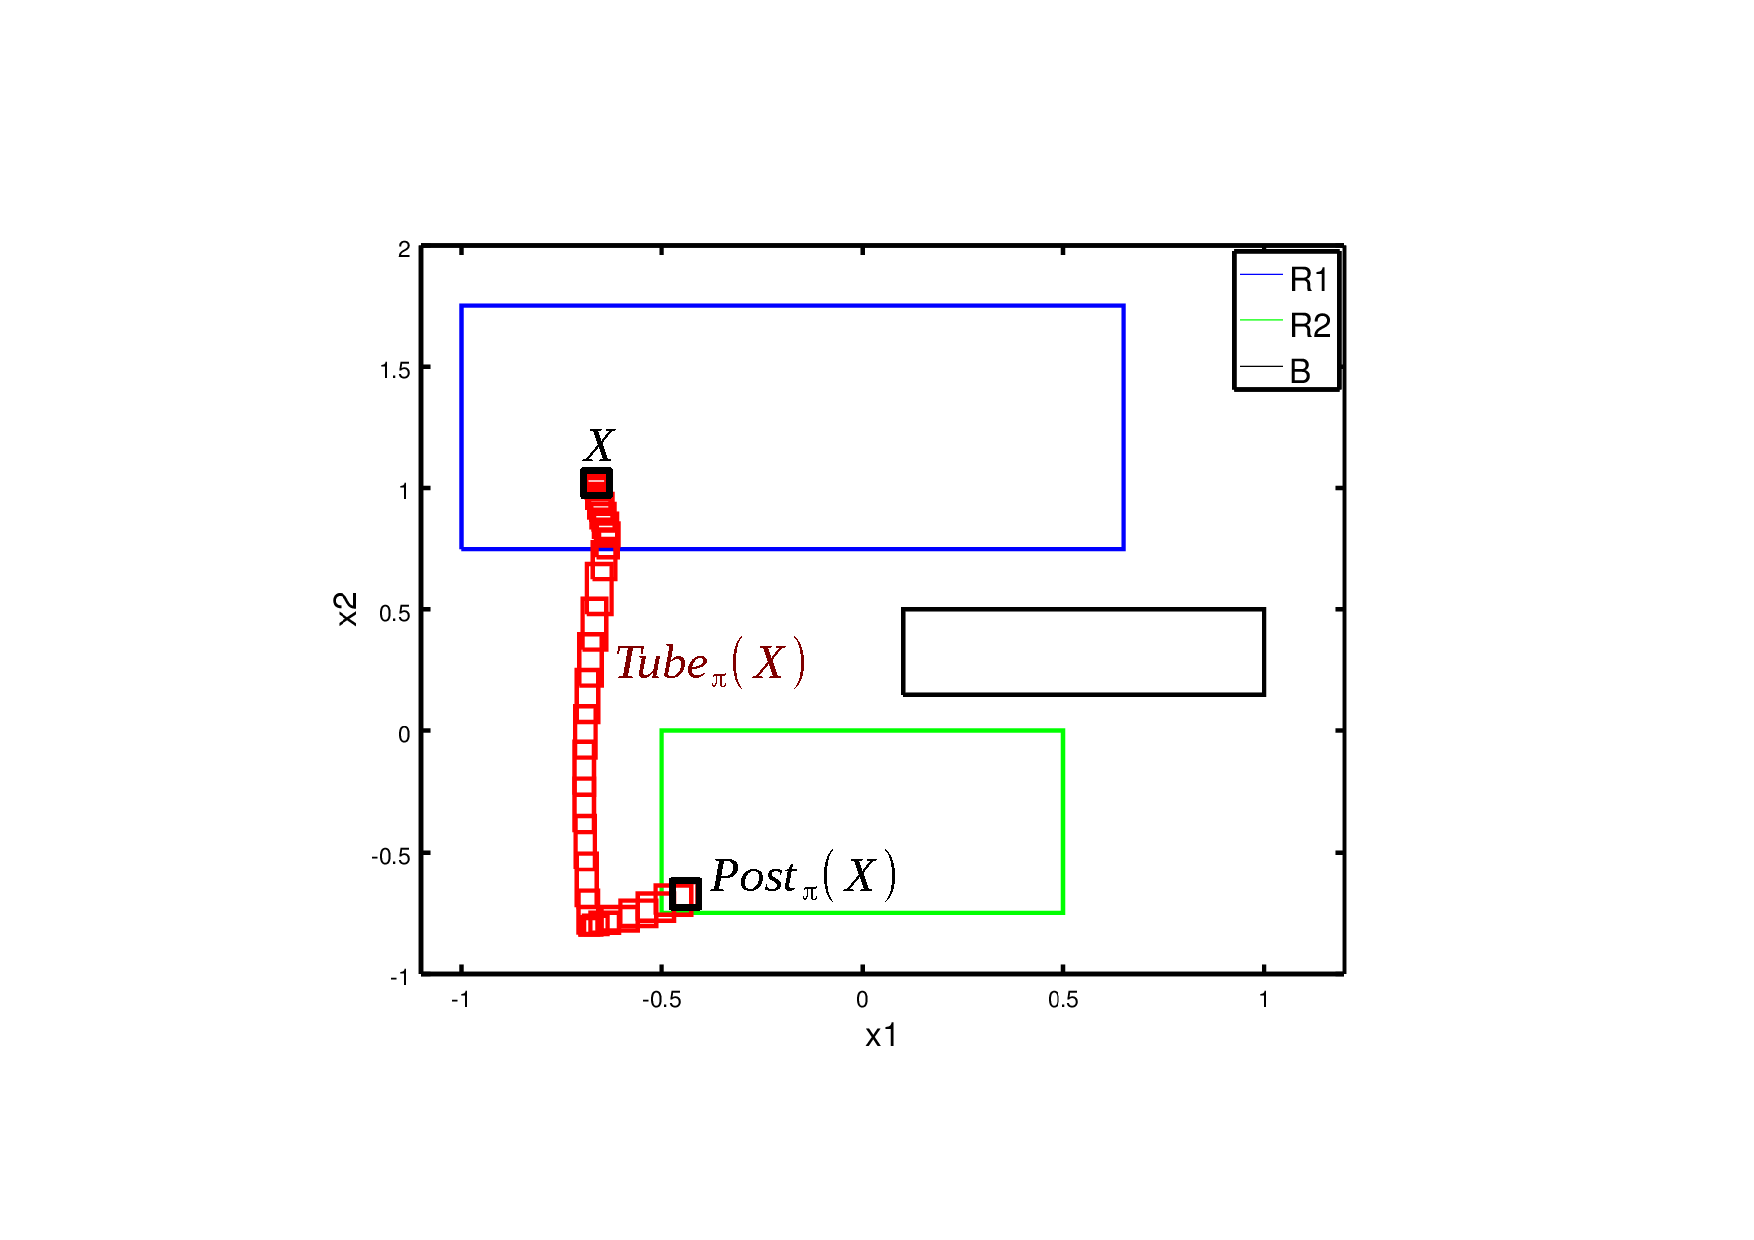
\includegraphics[%trim = 4cm 3cm 4cm 4cm, clip,
 width=0.5\textwidth]{tube.pdf}
 \caption{Functions $Post_{\pi}(X)$ and $Tube_{\pi}(X)$ for the
   initial box $X=[-0.69,-0.64] \times [1,1.06]$, with a pattern $\pi
   = (1,3,0)$.}
 \label{fig:post_tube}
\end{figure}

For a given pattern of switched modes $\pi = (i_1,\dots,i_k) \in U^k$
of length $k$, we are able to compute, for $j \in \{1,..,k\}$, the
enclosures:
\begin{itemize}
\item $[x_j] \ni x(j\tau)$;
\item $[\tilde{x}_j] \ni x(t), \ \text{for} \ t \in \lbrack
  (j-1)\tau,j\tau\rbrack$.
\end{itemize}
with respect to the system of IVPs:
\begin{equation}
  \left\{
    \begin{array}{c}
      \dot x(t) = f_{\sigma (t)}(t,x(t),d(t)),\\
      \nonumber x(t_0=0) \in [x_0] , d(t) \in [d],\\
      \sigma(t) = i_1, \forall t \in [0,t_1], t_1=\tau\\
      \vdots\\
      \dot x(t) = f_{\sigma (t)}(t,x(t),d(t)),\\
      \nonumber x(t_{k-1}) \in [x_{k-1}], d(t) \in [d],\\
      \sigma(t) = i_k, \forall t \in [t_{k-1},t_k], t_k=k\tau
    \end{array}
  \right.
\end{equation}
Thereby, the enclosure $Post_{\pi}(\lbrack x_0 \rbrack)$ is included
in $[x_k]$ and $Tube_{\pi}(\lbrack x_0 \rbrack)$ is included in
$\bigcup_{j=1,..,k} [\tilde{x}_j]$. This applies for all initial
states in $\lbrack x_0 \rbrack$ and all disturbances $d(t) \in [d]$. A
view of enclosures computed by the validated simulation for one
solution obtained for Example~\ref{ex2} is shown in
Figure~\ref{fig:post_tube}.



\subsubsection{Control synthesis}

If we now associate computation of the Post and Tube operators
to Algorithm \ref{algo:decomposition} and \ref{algo:findpattern2}, 
and using Theorem \ref{th:RS-procedure}, we can now perform control synthesis
ensuring $(R,S)$-stability, as well as $(R_1,R_2,S)$-reachability
and $(R,B,S)$-avoidance. 


\subsection{Experimentations}
\label{sec:experimentations}
%
In this subsection, we apply our approach to different case studies taken
from the literature.  Our solver prototype is written in C++ and based
on DynIBEX \cite{dynibex}.  The computations times given in the
following have been performed on a 2.80 GHz Intel Core i7-4810MQ CPU
with 8 GB of memory. Note that our algorithm is mono-threaded so all
the experimentation only uses one core to perform the computations.
The results given in this subsection have been obtained with Function
$Find\_Pattern2$.

\subsubsection{A linear example: boost DC-DC converter}

This linear example is taken from \cite{beccuti2005optimal} and has
already been treated with the state-space bisection method in a linear
framework in \cite{fribourg2014finite}. This running example is used to verify that our
approach is still valid for linear case, and also to show the strong improvement in term of computation time.

The system is a boost DC-DC converter with one switching cell.  There
are two switching modes depending on the position of the switching
cell. The dynamics is given by the equation $\dot x (t) =
A_{\sigma(t)} x(t) + B_{\sigma(t)}$ with $\sigma(t) \in U = \{ 1,2
\}$. The two modes are given by the matrices:

\begin{displaymath}
  A_1 = \left( \begin{matrix}
      - \frac{r_l}{x_l} & 0 \\ 0 & - \frac{1}{x_c} \frac{1}{r_0 + r_c}
    \end{matrix} \right)  \quad B_1 = \left( \begin{matrix}
      \frac{v_s}{x_l} \\ 0 \end{matrix} \right)
\end{displaymath}

\begin{displaymath}
  A_2 = \left( \begin{matrix} - \frac{1}{x_l} (r_l +
      \frac{r_0.r_c}{r_0 + r_c}) & - \frac{1}{x_l} \frac{r_0}{r_0 + r_c}
      \\ \frac{1}{x_c}\frac{r_0}{r_0 + r_c} & - \frac{1}{x_c}
      \frac{r_0}{r_0 + r_c}
    \end{matrix} \right)  \quad B_2 = \left( \begin{matrix}
      \frac{v_s}{x_l} \\ 0 \end{matrix} \right)
\end{displaymath}
with $x_c = 70$, $x_l = 3$, $r_c = 0.005$, $r_l = 0.05$, $r_0 = 1$,
$v_s = 1$.  The sampling period is $\tau = 0.5$.  The parameters are
exact and there is no perturbation.  We want the state to return
infinitely often to the region $R$, set here to $\lbrack 1.55 , 2.15
\rbrack \times \lbrack 1.0 , 1.4 \rbrack$, while never going out of
the safety set $S = \lbrack 1.54 , 2.16 \rbrack \times \lbrack 0.99 ,
1.41 \rbrack$.  The goal of this example is then to synthesize a
controller with intrinsic stability.

The decomposition was obtained in less than one second with a maximum
length of pattern set to $K = 6$ and a maximum bisection depth of $D =
3$.  A simulation is given in Figure~\ref{fig:NL_0}.

\begin{figure}[t]
 \centering
 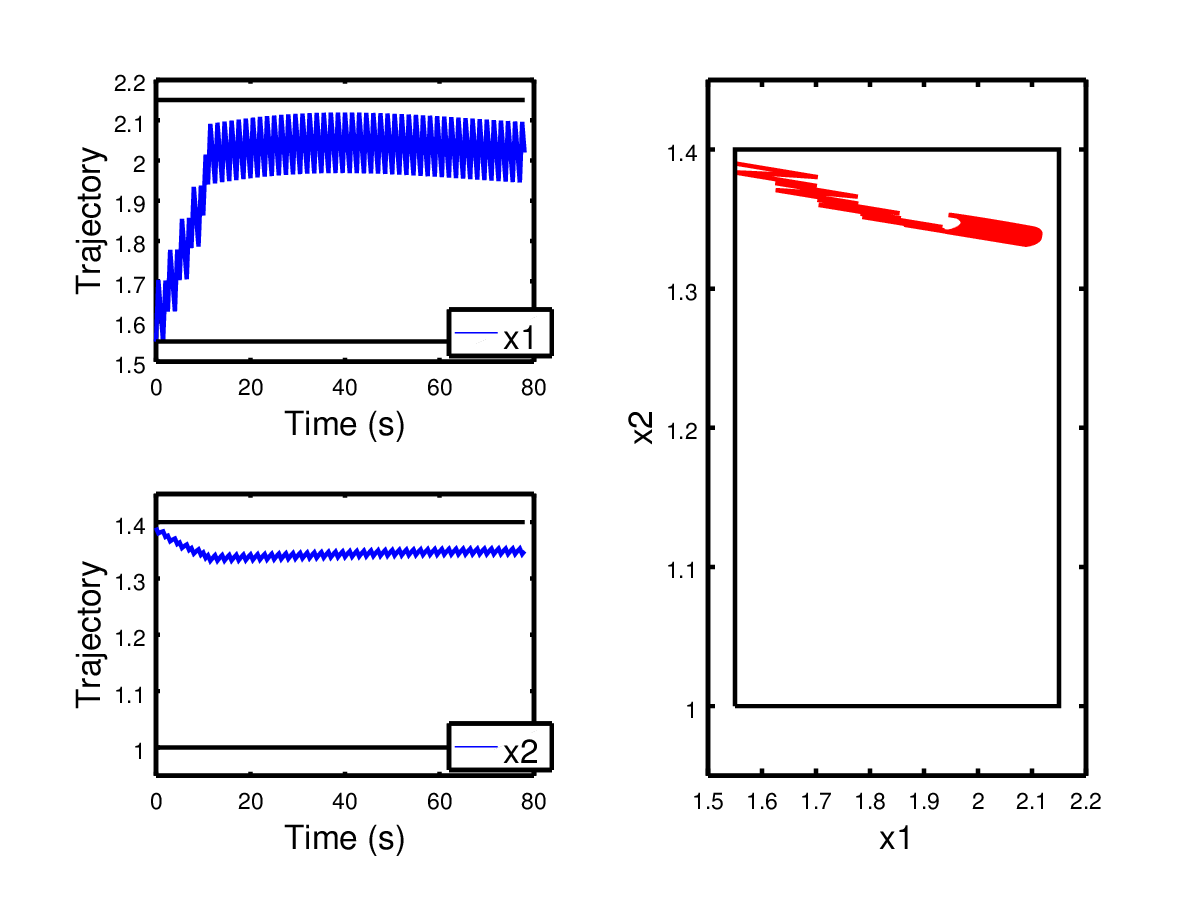
\includegraphics[scale=0.45]{simu_boost_safe.png}
 \caption{Simulation from the initial condition $(1.55,1.4)$. The box
   $R$ is in plain black. The trajectory is plotted within time for
   the two state variables on the left, and in the state-space plane
   on the right.}
  \label{fig:NL_0}
\end{figure}


\subsubsection{A polynomial example}
\label{ex2}
%
%
We consider the polynomial system taken from \cite{liu2013synthesis},
presented as a difficult example:
%
\begin{equation}
 \left \lbrack \begin{matrix}
  \dot x_1 \\ \dot x_2
 \end{matrix} \right \rbrack  =
 \left \lbrack \begin{matrix} -x_2 - 1.5 x_1 - 0.5 x_1^3 + u_1 + d_1 \\ x_1 + u_2 + d_2
   \end{matrix} \right \rbrack.
\end{equation}
%
The control inputs are given by $u = (u_1,u_2) =
K_{\sigma(t)}(x_1,x_2)$, $\sigma(t) \in U = \{ 1,2,3,4 \}$, which
correspond to four different state feedback controllers $K_1(x) =
(0,-x_2^2 + 2)$, $K_2(x) = (0,-x_2)$, $K_3(x) = (2,10)$, $K_4(x) =
(-1.5,10)$.  We thus have four switching modes. The disturbance $d =
(d_1,d_2)$ lies in $\lbrack -0.005,0.005 \rbrack \times \lbrack
-0.005,0.005 \rbrack$.  The objective is to visit infinitely often two
zones $R_1$ and $R_2$, without going out of a safety zone $S$, and
while never crossing a forbidden zone $B$.  Two decompositions are
performed:
\begin{itemize}
\item a decomposition of $R_1$ which returns $\{ (V_i,\pi_i) \}_{i
    \in I_1}$ with:
  \begin{itemize}
  \item $\bigcup_{i \in I_1} V_i = R_1$,
  \item $\forall i \in I_1, \ Post_{\pi_i}(V_i) \subseteq R_2$,
  \item $\forall i \in I_1, \ Tube_{\pi_i}(V_i) \subseteq S$,
  \item $\forall i \in I_1, \ Tube_{\pi_i}(V_i) \bigcap B = \emptyset$.
  \end{itemize}
\item a decomposition of $R_2$ which returns $\{ (V_i,\pi_i) \}_{i \in
    I_2}$ with:
  \begin{itemize}
  \item $\bigcup_{i \in I_2} V_i = R_2$,
  \item $\forall i \in I_2, \ Post_{\pi_i}(V_i) \subseteq R_1$,
  \item $\forall i \in I_2, \ Tube_{\pi_i}(V_i) \subseteq S$,
  \item $\forall i \in I_2, \ Tube_{\pi_i}(V_i) \bigcap B = \emptyset$.
  \end{itemize}
\end{itemize}

The input boxes are the following:
\begin{itemize}
\item $R_1 = \lbrack -0.5 , 0.5 \rbrack \times \lbrack -0.75 , 0.0
  \rbrack$,
\item $R_2 = \lbrack -1.0 , 0.65 \rbrack \times \lbrack 0.75 , 1.75
  \rbrack$,
\item $S = \lbrack -2.0 , 2.0 \rbrack \times \lbrack -1.5 , 3.0
  \rbrack$,
\item $B = \lbrack 0.1 , 1.0 \rbrack \times \lbrack 0.15 , 0.5
  \rbrack$.
\end{itemize}
The sampling period is set to $\tau = 0.15$. The decompositions were
obtained in $2$ minutes and $30$ seconds with a maximum length of
pattern set to $K = 12$ and a maximum bisection depth of $D = 5$.  A
simulation is given in Figure~\ref{fig:NL_1} in which the disturbance
$d$ is chosen randomly in $\lbrack -0.005,0.005 \rbrack \times \lbrack
-0.005,0.005 \rbrack$ at every time step.

\begin{figure}[t]
 \centering
 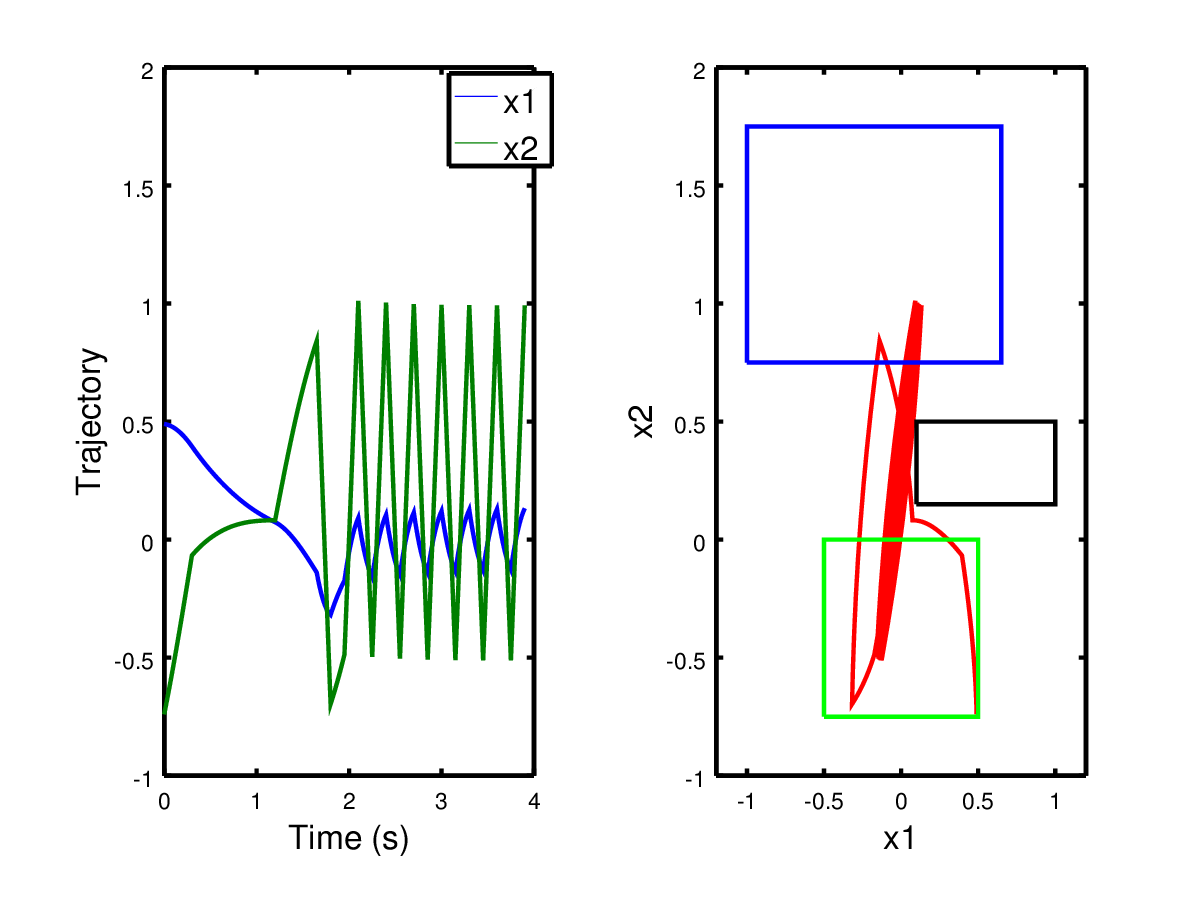
\includegraphics[scale=0.4]{simu_obstacle5.png}
 \caption{Simulation from the initial condition $(0.5,-0.75)$. The
   trajectory is plotted within time on the left, and in the state
   space plane on the right.  In the sate space plane, the set $R_1$
   is in plain green, $R_2$ in plain blue, and $B$ in plain black.}
 \label{fig:NL_1}
\end{figure}

\subsubsection{Building ventilation}
%
We consider a building ventilation application adapted from
\cite{meyer:tel-01232640}.  The system is a four room apartment
subject to heat transfer between the rooms, with the external
environment, with the underfloor, and with human beings.  The dynamics
of the system is given by the following equation:
\begin{displaymath}
 \frac{d T_i}{dt} = \sum_{j \in \mathcal{N}^\text{*}\setminus \{i\}} a_{ij} (T_j -
 T_i) + \delta_{s_i} b_i (T_{s_i}^4 - T_i ^4 ) + c_i
 \max\left(0,\frac{V_i - V_i^\text{*}}{\bar{ V_i} -
   V_i^{\text{*}}}\right)(T_u - T_i).
\end{displaymath}

The state of the system is given by the temperatures in the rooms
$T_i$, for $i \in \mathcal{N} = \{ 1 , \dots , 4 \}$.  Room $i$ is
subject to heat exchange with different entities stated by the indexes
$\mathcal{N}^\text{*} = \{1,2,3,4,u,o,c \}$.

\begin{figure}[t]
  \centering
  \includegraphics[scale=0.4]{NL_case_2_perturbation.png}
  \caption{Perturbation (presence of humans) imposed within time in the
    different rooms.}
  \label{fig:NL_2_perturbation}
\end{figure}


The heat transfer between the rooms is given by the coefficients
$a_{ij}$ for $i,j \in \mathcal{N}^2$, and the different perturbations
are the following:
\begin{itemize}
 \item The external environment: it has an effect on room $i$ with the
   coefficient $a_{io}$ and the outside temperature $T_o$, varying
   between $27^\circ C$ and $30^\circ C$.
  \item The heat transfer through the ceiling: it has an effect on
    room $i$ with the coefficient $a_{ic}$ and the ceiling temperature
    $T_c$, varying between $27^\circ C$ and $30^\circ C$.
  \item The heat transfer with the underfloor: it is given by the
    coefficient $a_{iu}$ and the underfloor temperature $T_u$, set to
    $17^\circ C$ ($T_u$ is constant, regulated by a PID controller).
  \item The perturbation induced by the presence of humans: it is
    given in room $i$ by the term $\delta_{s_i} b_i (T_{s_i}^4 - T_i
    ^4 )$, the parameter $\delta_{s_i}$ is equal to $1$ when someone
    is present in room $i$, $0$ otherwise, and $T_{s_i}$ is a given
    identified parameter.
\end{itemize}

\begin{figure}[t]
  \centering
  \includegraphics[scale=0.4]{NL_case_2.png}
  \caption{Simulation from the initial condition $(22,22,22,22)$. The
    objective set $R$ is in plain black and the safety set $S$ is in
    dotted black.}
  \label{fig:NL_2}
\end{figure}

The control $V_i$, $i \in \mathcal{N}$, is applied through the term
$c_i \max(0,\frac{V_i - V_i^\text{*}}{\bar{ V_i} -
  V_i^{\text{*}}})(T_u - T_i)$.  A voltage $V_i$ is applied to force
ventilation from the underfloor to room $i$, and the command of an
underfloor fan is subject to a dry friction.  Because we work in a
switched control framework, $V_i$ can take only discrete values, which
removes the problem of dealing with a ``max'' function in interval
analysis. In the experiment, $V_1$ and $V_4$ can take the values $0$V
or $3.5$V, and $V_2$ and $V_3$ can take the values $0$V or $3$V. This
leads to a system of the form of Equation~\eqref{eq:sys} with
$\sigma(t) \in U =\{ 1, \dots, 16 \}$, the $16$ switching modes
corresponding to the different possible combinations of voltages
$V_i$.  The sampling period is $\tau = 10$s.

The parameters $T_{s_i}$, $V_i^\text{*}$, $\bar V_i$, $a_{ij}$, $b_i$,
$c_i$ are given in \cite{meyer:tel-01232640} and have been identified
with a proper identification procedure detailed in
\cite{meyer2014ecc}.  Note that here we have neglected the term
$\sum_{j \in \mathcal{N}} \delta_{d_{ij}}c_{i,j} \ast h(T_j - T_i)$ of
\cite{meyer:tel-01232640}, representing the perturbation induced by
the open or closed state of the doors between the rooms. Taking a
``max'' function into account with interval analysis is actually still
a difficult task. However, this term could have been taken into
account with a proper regularization (smoothing).

The main difficulty of this example is the large number of modes in
the switched system, which induces a combinatorial issue.

The decomposition was obtained in $4$ minutes with a maximum length of
pattern set to $K = 2$ and a maximum bisection depth of $D = 4$.  The
perturbation due to human beings has been taken into account by
setting the parameters $\delta_{s_i}$ equal to the whole interval
$\lbrack 0,1 \rbrack$ for the decomposition, and the imposed
perturbation for the simulation is given
Figure~\ref{fig:NL_2_perturbation}.  The temperatures $T_o$ and $T_c$
have been set to the interval $\lbrack27,30\rbrack$ for the
decomposition, and are set to $30^\circ C$ for the simulation.  A
simulation of the controller obtained with the state-space bisection
procedure is given in Figure~\ref{fig:NL_2}, where the control
objective is to stabilize the temperature in $\lbrack 20 , 22 \rbrack
^4$ while never going out of $\lbrack 19 , 23 \rbrack ^4$.

\subsubsection{A path planning problem}


This last case study is based on a model of a vehicle initially
introduced in \cite{astrom2010feedback} and successfully controlled in
\cite{zamani2012symbolic,reissig2015feedback} with the tools PESSOA
and SCOTS. In this model, the motion of the front and rear pairs of
wheels are approximated by a single front wheel and a single rear
wheel. The dynamics if the vehicle is given by:
\begin{equation}
 \begin{array}{ccc}
  \dot x & = & v_0 \frac{\cos(\alpha + \theta)}{\cos(\alpha)} \\
  \dot y & = & v_0 \frac{\sin(\alpha + \theta)}{\cos(\alpha)} \\
  \dot \theta & = & \frac{v_0}{b} \tan(\delta)
  \end{array}
\end{equation}
where $\alpha = \arctan( a \tan (\delta) / b)$. The system is thus of
dimension $3$, $(x,y)$ is the position of the vehicle, while $\theta$
is the orientation of the vehicle.  The control inputs are $v_0$, an
input velocity, and $\delta$, the steering angle of the rear wheel.
The parameters are: $a=0.5$, $b=1$.  Just as in
\cite{zamani2012symbolic,reissig2015feedback}, we suppose that the
control inputs are piecewise constant, which leads to a switched
system of the form of Equation~\eqref{eq:sys} with no perturbation.
The objective is to send the vehicle into an objective region $R_2 =
[9,9.5]\times[0,0.5]\times ]-\infty,+\infty[$ from an initial region
$R_1 = [0,0.5]\times[0,0.5]\times[0,0]$. The safety set is $S = [0,10]
\times [0,10] \times]-\infty,+\infty[$.  There is in fact no
particular constraint on the orientation of the vehicle, but multiple
obstacles are imposed for the two first dimensions, they are
represented in Figure \ref{fig:unicycle}. The input velocity $v_0$ can
take the values in $\{-0.5,0.5,1.0\}$. The rear wheel orientation
$\delta$ can take the values in
$\{0.9,0.6,0.5,0.3,0.0,-0.3,-0.5,-0.6,-0.9\}$. The sampling period is
$\tau = 0.3$.

\begin{figure}[t]
  \centering
  \includegraphics[scale=0.5% ,clip,trim=0cm 6.5cm 0cm 6.5cm
  ]{unicycle_sol.pdf}
  \caption{Set simulation of the path planning example. The green box
    is the initial region $R_1$, the blue box is the target region
    $R_2$. The union of the red boxes is the reachability tube. In
    this case, the target region is not attained without bisection.}
  \label{fig:unicycle}
\end{figure}


\begin{figure}[t]
  \centering
  \begin{tabular}{cc}
    \includegraphics[width=0.35\textwidth,clip,trim=0cm 0cm 0cm 0cm]{uni1.png}
    &
    \includegraphics[width=0.35\textwidth,clip,trim=0cm 0cm 0cm 0cm]{uni2.png}
    \\
    \includegraphics[width=0.35\textwidth,clip,trim=0cm 0cm 0cm 0cm]{uni3.png}
    &
    \includegraphics[width=0.35\textwidth,clip,trim=0cm 0cm 0cm 0cm]{uni4.png}
  \end{tabular}
  \caption{Set simulation of the path planning example after
    bisection. The green boxes are the initial regions obtained by
    bisection, the blue box is the target region $R_2$. The union of
    the red boxes is the reachability tube.}
  \label{fig:unicycle2}
\end{figure}


Note that for this case study we used an automated pre-tiling of the
state-space permitting to decompose the reachability problem in a
sequence of reachability problems.  Using patterns of length up to
$K=10$, we managed to successfully control the system in $3619$
seconds. In this case, the pattern is computed until almost the end
without bisection as shown in Figure~\ref{fig:unicycle}. To obtain the
last steps, the box is bissected in four ones by
Algorithm~\ref{algo:decomposition}. After that, patterns are found for
the four boxes:
\begin{itemize}
 \item $[8.43, 8.69] ; [2.52, 2.78] : \{7 0 0 0 1 6 6 \}$
 \item $[8.43, 8.69] ; [2.78, 3.03] : \{7 0 0 0 2 5 6 \}$
 \item $[8.69, 8.94] ; [2.52, 2.78] : \{0 0 0 5 5 \}$
 \item $[8.69, 8.94] ; [2.78, 3.03] : \{0 0 0 2 6 5 \}$
\end{itemize}

The four set simulations obtained for the last steps are given in
Figure~\ref{fig:unicycle2}.


\subsection{Performance tests}
\label{sec:comparison}

We present a comparison of functions $Find\_Pattern$, $Find\_Pattern2$
w.r.t. the computation times obtained, and with the state-of-the-art
tools PESSOA \cite{Mazo2010} and SCOTS \cite{SCOTS}.


Table~\ref{tab:FP1-FP2} shows a comparison of functions
$Find\_Pattern$ and $Find\_Pattern2$, which shows that the new version
highly improves computation time.  We can note that the new
version is all the more efficient as the length of the patterns
increases, and as obstacles cut the research tree of patterns. This is
why we observe significant improvements on the examples of the DC-DC
converter and the polynomial example, and not on the building
ventilation example, which only requires patterns of length $2$, and
presents no obstacle.

\begin{table}[t]
  \centering
  \caption{Comparison of $Find\_Pattern$ and $Find\_Pattern2$.}
  \label{tab:FP1-FP2}
  \begin{tabular}{|c|c|c|}
    \hline
    Example & \multicolumn{2}{c|}{Computation time} \\
    \cline{2-3} & $~Find\_Pattern~$ & $~Find\_Pattern2~$   \\
    \hline
    DC-DC Converter &    $1609$ s  &  $< 1$ s \\
    Polynomial example & Time Out   & $150$ s  \\
    Building ventilation & $272$ s & $228$ s  \\
    Path planning & Time Out & $3619$ s \\
    \hline
  \end{tabular}
\end{table}

Table~\ref{tab:SOTA} shows of comparison of function $Find\_Pattern2$
with state-of-the-art tools SCOTS and PESSOA.  On the example of the
DC-DC converter, our algorithm manages to control the whole
state-space $R=\lbrack 1.55 , 2.15 \rbrack \times \lbrack 1.0 , 1.4
\rbrack$ in less than one second, while SCOTS and PESSOA only control
a part of $R$, and with greater computation times. Note that these
computation times vary with the number of discretization points used
in both, but even with a very fine discretization, we never managed to
control the whole box $R$.  For the polynomial example, we manage to
control the whole boxes $R_1$ and $R_2$, such as SCOTS and in a
comparable amount of time. However, PESSOA does not support natively
this kind of nonlinear systems. For path planning case study, on which
PESSOA and SCOTS perform well, we have not obtained as good
computations times as they have.  This comes from the fact that this
example requires a high number of switched modes, long patterns, as
well as a high number of boxes to tile the state-space.  This is in
fact the most difficult case of application of our method.  This
reveals that our method is more adapted when either the number of
switched modes of the length of patterns is not high (though it can be
handled at the cost of high computation times).  Another advantage is
that we do not require a homogeneous discretization of the state
space. We can thus tile large parts of the state-space using only few
boxes, and this often permits to consider much less symbolic states
than with discretization methods, especially in higher dimensions (see
\cite{LeCoent2016}).


\begin{table}[t]
  \centering
  \caption{Comparison with state-of-the-art tools.}
  \label{tab:SOTA}
  \begin{tabular}{|c|c|c|c|}
    \hline
    Example & \multicolumn{3}{c|}{Computation time} \\
    \cline{2-4} & ~FP2~ & ~SCOTS~ & ~PESSOA~   \\
    \hline
    DC-DC Converter & $< 1$ s &    $43$ s  &  $760$ s \\
    Polynomial example & $150$ s & $131$ s & $\_\_$  \\
    Path planning & $3619$ s & $492$ s & $516$ s \\
    \hline
  \end{tabular}
\end{table}


\subsection{Conclusion}
\label{sec:conclu}

We presented a method of control synthesis for nonlinear switched
systems, based on a simple state-space bisection algorithm, and on
validated simulation. The approach permits to deal with stability,
reachability, safety and forbidden region constraints. Varying
parameters and perturbations can be easily taken into account with
interval analysis. The approach has been numerically validated on
several examples taken from the literature, a linear one with constant
parameters, and two nonlinear ones with varying perturbations.  Our
approach compares well with the state-of-the art tools SCOTS and
PESSOA.

We would like to point out that the exponential complexity of the
algorithms presented here, which is inherent to guaranteed methods, is
not prohibitive. Two approaches have indeed been developed to overcome
this exponential complexity.  A first approach is the use of
compositionality, which permits to split the system in two (or more)
sub-systems, and to perform control synthesis on these sub-systems of
lower dimensions.  This approach has been successfully applied in
\cite{LeCoent2016} to a system of dimension $11$, and we are currently
working on applying this approach to the more general context of
contract-based design \cite{sangiovanni2012taming}.  A second approach
is the use of Model Order Reduction, which allows to approximate the
full-order system \eqref{eq:sys} with a reduced-order system, of lower
dimension, on which it is possible to perform control synthesis.  The
bounding of the trajectory errors between the full-order and the
reduced-order systems can be taken into account, so that the induced
controller is guaranteed. This approach, described in
\cite{le2016control}, has been successfully applied on
(space-discretized) partial differential equations, leading to systems
of ODEs of dimension up to $100 000$.  The present work is a potential
ground for the application of such methods to control of nonlinear
partial differential equations, with the use of proper nonlinear model
order reduction techniques.




\section{Sampled switched systems with one-sided Lipschitz conditions}\label{sec:OSL}
\subsection{Lipschitz and one-sided Lipschitz condition}\label{ss:OSC}
Let us consider a nonlinear switched system of the form \eqref{eq:switched_system0}.
We make the following hypothesis:
%
$$(H0)\quad  \mbox{ For all  $j\in U$, $f_j$ is a locally Lipschitz continuous map}.$$
%
As in \cite{girard2010approximately}, we make the assumption that 
the vector field $f_j$ is such that the solutions of the 
differential equation  (\ref{eq:switched_system0}) are defined, 
e.g. by assuming that the support of the vector field $f_j$ is compact.
% We will denote by $\phi_\sigma(t;x^0)$ the 
% solution at time~$t$ of the system:
% 
% \begin{equation}
% \begin{aligned}
%   \dot x(t) & = f_{\sigma (t)}(x(t)), \\
%   x(0) & =  x^0. \\
% %  \sigma(t) & =  j \in U \ \text{for} \ t
% %  \in \lbrack k\tau , (k+1)\tau ),\ \ k=0,1,\dots
% \end{aligned}
%  \label{eq:ssampled-sys_part2}
% \end{equation}
%


%that the system is in a given mode $\sigma(t) =\sigma = j \in U$, 
%we abbreviate, for $t \in [0,\tau )$, $x_\sigma(t) = \phi(t;x^0,\sigma)$.
%%as well as $\tilde x_\sigma(t) = \tilde \phi_{\tilde x^0}(t;\tilde x^0,\sigma)$.

%\begin{remark}
%Definir $\phi$ pour pattern $\pi$ et $0\leq t <k\tau$ (ou $0\leq t \leq k\tau$).
%\end{remark}

We denote by $T$ a compact overapproximation of the image by $\phi_j$ of $S$ for $0\leq t\leq \tau$ and $j\in U$, i.e.~$T$ is such that
$$ T\supseteq \{\phi_j(t;x^0) \ |\ j\in U, 0\leq t\leq\tau, x^0\in S\}.$$
%%%%
The existence of $T$ is guaranteed by assumption $(H0)$. We know furthermore 
by $(H0)$ that, for all $j\in U$, there exists a constant $L_j>0$ such that:
%\label{hyp:2}
%For all $j \in U$, there exists a constant $L_j>0$ such that
\begin{equation}
\| f_j(y)-f_j(x) \| \leq L_j \, \|y-x\|\quad \forall x,y\in S.
\label{eq:lipschitz}
\end{equation}
Let us define $C_j$ for all $j\in U$:
%We have:
\begin{equation}
%L\|f_{j}(x)\|\leq C_0 
C_j = \sup_{x\in S}\  L_j\|f_j(x)\|
\quad
\text{for all} \quad j\in U.
\label{eq:L}
\end{equation}
%
We make the additional hypothesis 
that the mappings $f_j$ are {\em one-sided Lipschitz} (OSL)
\cite{Donchev98}.

%, which are often verified on systems modeling
%real world applications such as temperature regulation in a building (eg., \cite{meyer2014ecc}):
%we consider 
%%%The Lipschitz condition is classically assumed in order to 
% ensure the existence of a (unique) integral solution $\phi_\sigma$
%(see, e.g., \cite{liberzon2012switching}). 
%This assumption of strong monotony is original in the context of switched systems, as far as we know. 
Formally:
%
$$(H1) 
%\label{hyp:1}
\quad \mbox{ For all $j \in U$, there exists a constant $\lambda_j\in \mathbb{R}$ such that}$$ 
\[
\langle f_j(y)-f_j(x), y-x \rangle \leq \lambda_j\, \|y-x\|^2\quad
\forall x,y\in T,
\]
where $\langle \cdot, \cdot\rangle$ denotes the scalar product of two vectors of $\mathbb{R}^n$.
%\end{definition}
%
%\footnote{Let  $\lambda_{min} = \min_{j \in U} \lambda_j$.}
Constant $\lambda_j \in \R$ is called one-sided Lipschitz (OSL) constant, and can also be found in the 
literature as Dahlquist's constant [ref???].
Note that in practice, hypotheses H0 and H1 are not strong. 
Hypothesis H0 just ensures the existence of solutions for system,
and constants $L_j$ and $\lambda_j$ can always be found if the state 
of the system stays in a compact (e.g. the set $T$).
%have (in the case of linear equations) eigenvalues of very different modulus.
%The stability of systems governed by stiff equations is difficult to establish using only  Lipschitz constants.\footnote{The Euler method can also be numerically unstable, especially for stiff equations, meaning that the numerical solution grows very large for equations where the exact solution does not (Wikipedia).}
%

\paragraph{Computation of constants $\lambda_j$, $L_j$ and $C_j$}

The computation of constants $L_j$, $C_j$, $\lambda_j$ 
($j\in U$) are realized with
a constrained optimization algorithm.
They are performed using the ``sqp'' function of Octave, applied on the following 
optimization problems:
\begin{itemize}
 \item Constant $L_j$:
 $$ L_j = \max_{{x,y}\in S,\  x\neq y} \frac{\| f_j(y) - f_j(x) \|}{\| y - x \|}  $$
 \item Constant $C_j$:
 $$ C_j = \max_{{x}\in S} L_j \| f_j(x) \|$$
 \item Constant $\lambda_j$:
 $$ \lambda_j = \max_{{x,y}\in T,\  x\neq y} \frac{\langle f_j(y) - f_j(x), y - x \rangle}{\|y - x \|^2 }$$
 \end{itemize}
We could point out that the computation of the constants is not guaranteed, in the 
sense that the results given by optimization algorithms does not 
provide a guarantee that an overapproximation of the constants is computed. However,
some works have been done for computing over and under approximation
of Lipschitz constants in \cite{} [???], and could be used here. This approach can 
be extended to the OSL constant. In the following, we consider that we can 
compute these constants exactly.
 
 
\paragraph{Origin of the OSL property}

This notion has been used for the first time by \cite{donchev1998stability}
in order to treat ``stiff'' systems of differential equations for which the explicit Euler method is
numerically ``unstable'' (unless the step size is taken to be extremely small).
Unlike Lipschitz constants, OSL constants can be {\em negative}.
In the case where an OSL constant $\lambda_j$ is negative, it is said that the vector 
field $f_j$ is strongly monotone \cite{???},
which express a form of contractivity of the system dynamics: a strongly monotone system
presents trajectories getting exponentially closer together 
within time.
Even if the OSL constant is positive, it is in practice much lower than
the Lipschitz constant \cite{dahlquist1976error}. The use of OSL thus allows us to obtain a much
more precise upper bound for the global error.
We believe that this notion is also closely related to
the notion of incremental stability \cite{???}. We think that 
it could be shown that any system presenting a negative OSL constant is
incrementally stable, since it is already the case for linear systems.
Indeed, a system presenting a negative OSL constant actually admits $\| \cdot \|^2$ 
as a stable Lyapunov function \cite{???}.
However, this OSL Lipschitz property has never been used in the context of
switched systems and symbolic control. 



\subsection{A note on the OSL constant for linear systems}

We show here a result giving an exact expression for the OSL constant
for linear vector fields.

% \begin{equation}
%  \dot x = A_\sigma x + b_\sigma
%  \label{eq:switched_sys_linear}
% \end{equation}


% \begin{definition}[Strong monotony]
% %\label{hyp:1}
% Let $X \subset \mathbb{R}^n$ be a compact set. 
% A function $f: X \longrightarrow X$ is 
% said to be strongly monotone on $X$ if
% \[
% \exists \beta>0 \ \text{s.t.} \ \langle f(y)-f(x), y-x \rangle \geq \beta\, \|y-x\|^2\quad
% \forall x,y\in X,
% \]
% where $\langle \cdot, \cdot\rangle$ denotes the scalar product of $\mathbb{R}^n$.
% \end{definition}
\begin{proposition}
Let $X \subset \mathbb{R}^n$ be a (non trivial) compact set.
 Let $A \in \mathcal{M}_n (\mathbb{R})$, $b \in \mathbb{R}^n$ and $f(x)=A x + b$. 
 The OSL constant of $f$ is equal to the greatest eigenvalue of $\frac{A + A^\top}{2}$.
\end{proposition}
\vspace{1em}
\begin{proof}
%  Consider $f(x)=A x + b$.
First
\[
\exists \lambda \in \R \ \text{s.t.} \ \langle f(y)-f(x), y-x \rangle \leq \lambda\, \|y-x\|^2\quad
\forall x,y\in X,
\]
is equivalent to
\[
\exists \lambda \in \R \ \text{s.t.} \ \langle A(y-x), y-x \rangle \leq \lambda\, \|y-x\|^2\quad
\forall x,y\in X,
\]
and is equivalent to (the case $x = y$ being trivial)
\begin{equation}
\exists \lambda \in \R \ \text{s.t.} \ \langle A \frac{y-x}{\| y-x \|}, \frac{y-x}{\| y - x \|} \rangle \leq \lambda\ \quad
\forall x,y\in X, x \neq y, 
\label{eq:demo0}
\end{equation}
and it is thus equivalent to 
\begin{equation}
\exists \lambda \in \R \ \text{s.t.} \ \langle {Az}, {z} \rangle \leq \lambda\ \quad
\forall z \in S(0,1),
\label{eq:demo1}
\end{equation}
where $S(0,1)$ is the sphere of center $0$ and radius $1$ in $\mathbb{R}^n$, and because $X$ is non trivial.


Let us then remark that we have
\begin{equation}
\langle {Az}, {z} \rangle = \langle { \frac{A + A^\top}{2} z}, {z} \rangle
\label{eq:rem}
\end{equation}

Indeed, if $A = (a_{ij})_{ij}$ and $z = (z_i)_i$:
$$
\langle {Az}, {z} \rangle = \sum_{i=1}^n \sum_{j=1}^n z_i a_{ij} z_j  = \sum_{i=1}^n \sum_{j=1}^n a_{ij} z_i z_j
$$

$$
\langle {\frac{A+A^\top}{2}z}, {z} \rangle = \frac{1}{2} \left(\sum_{i=1}^n \sum_{j=1}^n a_{ij} z_i z_j +\sum_{i=1}^n \sum_{j=1}^n  a_{ji} z_i z_j \right) 
$$
The sums on the last term can be exchanged, it yields
$$
\langle {\frac{A+A^\top}{2}z}, {z} \rangle = \frac{1}{2} \left(\sum_{i=1}^n \sum_{j=1}^n a_{ij} z_i z_j +\sum_{j=1}^n \sum_{i=1}^n  a_{ji} z_i z_j \right) 
$$
$$
= \frac{1}{2} \left(\sum_{i=1}^n \sum_{j=1}^n a_{ij} z_i z_j +\sum_{i=1}^n \sum_{j=1}^n  a_{ij} z_i z_j \right) 
$$
$$
= \langle {A z}, {z} \rangle
$$

We thus have equivalence of \eqref{eq:demo1} and 
\begin{equation}
\exists \lambda\in \R \ \text{s.t.} \ \langle {\frac{A + A^\top}{2}z}, {z} \rangle \leq \lambda\ \quad
\forall z \in S(0,1),
\label{eq:demo2}
\end{equation}

Now, $\frac{A + A^\top}{2}$ is a symmetric matrix, let us denote by 
$\lambda_1^s$,$\dots$,$\lambda_n^s$ its (real) eigenvalues. Let us denote by $\lambda_{min}^s$
the minimum one, and by  $\lambda_{max}^s$ the maximum one. We can apply the known result 
(using for example Rayleigh quotient's properties \cite{???}):
$$ \forall z \in S(0,1),\ \lambda_{min}^s  \leq \langle {\frac{A + A^\top}{2}z}, {z} \rangle \leq \lambda_{max}^s  $$
and equality is attained in both sides for $z$ (normalized) eigenvector of $\frac{A + A^\top}{2}$ 
corresponding to eigenvalues $\lambda_{min}^s$ and $\lambda_{max}^s$, which proves the result.

% We finally have \eqref{eq:demo2} equivalent to $\lambda_{min}^s >0$, which proves the proposition.
% Moreover, the smallest $\lambda >0$ is $\lambda_{min}^s$.

\end{proof}


\begin{remark}
 Function $\phi: z \longrightarrow \langle Az, z \rangle$ is a quadratic form.
 It thus has a unique {\em symmetric} matrix $M$ such that $\phi(z) = \langle Mz,z \rangle$, 
 this unique symmetric matrix is $\frac{A + A^\top}{2}$.
\end{remark}


% \vspace{1em}

% \begin{remark}
% Constants $\lambda_j$, $L_j$ and $C_j$  ($j\in U$) can 
% be computed using (constrained) optimization algorithms. See
% Section \ref{sec:experiment} for details.
% %be computed with (constrained) optimization algorithms. 
% %In practice, they are computed before the synthesis step.
% %, using Octave functions.
% \end{remark}



%\begin{remark}
%%Suppose that $f_j$ is affine, i.e: $f_j(x)=A_j(x)+b_j$ for some matrix $A_j$ with real coefficients. Let us give a (necessary and) sufficient condition for $f_j$ to satisfy $(H1)$.\footnote{It is immediate that affine functions satisfy $(H0)$.} Using the fact that $\langle A_j x, x\rangle = \frac{1}{2}\langle (A_j+A_%j^\top)x, x\rangle$, it is easy to show that $f_j$ has a positive  one-sided Lipschitz constant iff the eigenvalues of $(A_j+A_j^\top)$ are all (real) positive.
%\end{remark}

\subsection{Euler approximate solutions}

Having defined OSL conditions, we now present an original method allowing 
to compute reachability sets and tubes, relying on the Euler method.
The introduction of OSL conditions actually allows to establish a
new global error bound, permitting the computation of overapproximation
of reachability sets and tubes, precise enough to be used for control synthesis. 


Given an  initial point $\tilde{x}^0\in S$ and a mode $j\in U$, 
we define the following ``linear approximate 
solution''~$\tilde{\phi}_j(t;\tilde{x}^0)$ for $t$ on $[0,\tau]$ by:
\begin{equation}
\tilde{\phi}_j(t;\tilde{x}^0) = \tilde x^0 + t f_j(\tilde x^0).
\label{eq:grossier}
\end{equation}
%for $\sigma(t)=j$.
\newline
\vspace{1em}
Note that formula~\eqref{eq:grossier} is nothing else but the explicit forward Euler scheme 
with ``time step'' $t$. It is thus a {consistent} approximation of order $1$ in $t$
of the exact trajectory of~\eqref{eq:switched_system0}
%$x_\sigma(t)$ 
under the hypothesis $\tilde x^0=x^0$.
% We further suppose that we have 
% \[
% \tilde x(t)\in R\quad \forall t\geq 0.
% \]
% %

More generally, given an initial point $\tilde{x}^0\in S$ and  pattern $\pi$ of $U^k$,
we can define a ``(piecewise linear) approximate solution'' 
$\tilde{\phi}_\pi(t;\tilde{x}^0)$ of $\phi_\pi$ at time $t\in[0,k\tau]$ as follows:
\begin{itemize}
\item $\tilde{\phi}_\pi(t;\tilde{x}^0) = t f_j(\tilde{x}^0) + \tilde{x}^0$ if $\pi=j\in U$, $k=1$ and $t\in[0,\tau]$, and

\item $\tilde{\phi}_{\pi}(k\tau+t;\tilde{x}^0) = t f_j(\tilde{z}) + \tilde{z}$
with $\tilde{z}=\tilde{\phi}_{\pi'}((k-1)\tau;\tilde{x}^0)$, if $k\geq 2$, 
$t\in[0,\tau]$,
$\pi=j\cdot \pi'$ for some $j\in U$ and $\pi'\in U^{k-1}$.
\end{itemize}

%{\bf NB: } We suppose that all the intermediate points $\tilde{z}$ belong to $S$ (\`a pr\'eciser)???.\\

We wish to synthesize a guaranteed control $\sigma$ for $\phi_{\sigma}$
using the approximate functions $\tilde{\phi}_\pi$.%\eqref{eq:grossier}. 
We define the closed ball of center $x\in\mathbb{R}^n$ and radius $r>0$, denoted $B(x,r)$, as the set $\{x'\in\mathbb{R}^n \ |\ \|x'-x\| \leq r\}$.

Given a positive real $\delta$, we now define the expression $\delta_j(t)$
which, as we will see in Theorem \ref{th:1}, represents (an upper bound on)
the error associated to $\tilde{\phi}_j(t; \tilde{x}^0)$
(i.e. $\|\tilde{\phi}_j(t; \tilde{x}^0)-\phi_j(t; x^0)\|$).

\begin{definition}\label{def:4}
%In case  $(H1)$ is not satisfied because $\lambda=\min_{j\in U} \lambda_j <0$, %(and $\delta \not\geq\frac{C_0\tau}{\lambda}$), 
%the conclusion of Theorem \ref{prop:bound} still holds if $B(\tilde{\phi}(t;\tilde{x}^0),\delta)$
%is replaced by $B(\tilde{\phi}(t;\tilde{x}^0),\delta'(t))$
%with 
Let $\delta$ be a positive constant. Let us define, for all $0\leq t\leq \tau$,
$\delta_j(t)$ as follows:
\begin{itemize}
\item  if $\lambda_j <0$:
$$\delta_j(t)=\left(\delta^2 e^{\lambda_j t}+
 \frac{C_j^2}{\lambda_j^2}\left(t^2+\frac{2 t}{\lambda_j}+\frac{2}{\lambda_j^2}\left(1- e^{\lambda_j t} \right)\right)\right)^{\frac{1}{2}}$$
%

\item if $\lambda_j = 0:$
$$\delta_j(t)= \left( \delta^2 e^{t} + C_j^2 (- t^2 - 2t + 2 (e^t - 1)) \right)^\frac{1}{2}$$




%\item if $\lambda_j = 0:$
%$$\delta_j(t)= \frac{C_j t^2}{2} + \delta$$

\item if $\lambda_j > 0:$
$$\delta_j(t)=\left(\delta^2 e^{3\lambda_j t}+
\frac{C_j^2}{3\lambda_j^2}\left(-t^2-\frac{2t}{3\lambda_j}+\frac{2}{9\lambda_j^2}
\left(e^{3\lambda_j t}-1\right)\right)\right)^{\frac{1}{2}}$$
%
\end{itemize}
\end{definition}

Note that $\delta_j(t)=\delta$ for $t=0$. 
The function $\delta_j(\cdot)$ depends implicitly on two parameters: $\delta\in\mathbb{R}$ and $j\in U$. In Section \ref{sec:appl}, we will use the notation $\delta'_j(\cdot)$
where the parameters are denoted by $\delta'$ and $j$.
%\footnote{In case $\lambda_j \geq 0$, the radius of the safety ball computed by our method increases exponentially with~$t$.}
%The proof is a simple adaptation of the above proof.


\begin{theorem}\label{th:1}

Given
a sampled switched system satisfying (H0-H1), consider
a point $\tilde{x}^0$
and a positive real $\delta$. 
We have,
for all $x^0\in B(\tilde{x}^0,\delta)$, $t\in [0,\tau]$ and  $j\in U$:

%$$\phi_j(t;x^0)\in B(\tilde{x}^0-t f_j(\tilde{x}^0), \gamma)$$ 
$\phi_j(t;x^0)\in B(\tilde{\phi}_j(t;\tilde{x}^0),\delta_j(t))$.
\end{theorem}



\begin{proof}


Consider on $t\in [0,\tau]$ the differential equations 
%
\[
\frac{d  x(t)}{dt} = f_j(x(t))
\]
and
\[
\frac{d \tilde x(t)}{dt} = f_j(\tilde x^0).
\]
with initial points $x^0\in S,\tilde{x}^0\in S$ respectively.
%
We will abbreviate $\phi_j(t;x^0)$ 
(resp. $\tilde{\phi}_j(t;\tilde{x}^0)$) as $x(t)$ (resp.~$\tilde{x}(t)$).
We have
\[
\frac{d}{dt}(x(t)-\tilde x(t)) =  \left( f_j(x(t))-f_j(\tilde x^0)\right),
\]
then
\begin{eqnarray*}
\frac{1}{2}\, \frac{d}{dt}(\|x(t)-\tilde x(t)\|^2) &=& 
\left\langle f_j(x(t))-f_j(\tilde x^0),  x(t)-\tilde x(t) \right\rangle \\ %[1.1ex]
%
&=& \left\langle f_j(x(t))-f_j(\tilde x(t))+f_j(\tilde x(t))
                      -f_j(\tilde x^0),  x(t)-\tilde x(t) \right\rangle\\
&=& \left\langle f_j(x(t))-f_j(\tilde x(t)), x(t)-\tilde x(t) \right\rangle
+\left\langle f_j(\tilde x(t))                      -f_j(\tilde x^0),  x(t)-\tilde x(t) \right\rangle\\
&\leq& \left\langle f_j(x(t))-f_j(\tilde x(t)), x(t)-\tilde x(t) \right\rangle
+ \| f_j(\tilde x(t))                      -f_j(\tilde x^0)\| \| x(t)-\tilde x(t) \|.
\end{eqnarray*}
%
The last expression has been obtained using the Cauchy-Schwarz inequality. Using $(H1)$ and (\ref{eq:lipschitz}), we have %the inequality
%\[
%\frac{1}{2}\, \frac{d}{dt}(\|x(t)-\tilde x(t)\|^2)
%\leq -\lambda \|x(t)-\tilde x(t)\|^2
%+\left\langle f_j(\tilde x(t))-f_j(\tilde x^0),  x_%j(t)-\tilde x(t) \right\rangle 
%\]
%%Applying Cauchy-Schwarz inequality on the last term then the Lipschitz property, we get
%
\begin{eqnarray*}
\frac{1}{2}\, \frac{d}{dt}(\|x(t)-\tilde x(t)\|^2)
&\leq& \lambda_j \|x(t)-\tilde x(t)\|^2
+\, \| f_j( \tilde x(t))- f_j(\tilde x^0)\|\,  \|x(t)-\tilde x(t)\|
 \\%[1.1ex]
%
&\leq& \lambda_j \|x(t)-\tilde x(t)\|^2
+L_j\, \|\tilde x(t)-\tilde x^0\|\,  \|x(t)-\tilde x(t)\| \\%[1.1ex]
%
&\leq& \lambda_j \|x(t)-\tilde x(t)\|^2
+L_j t\, \|f_j(\tilde x^0)\|\,  \|x(t)-\tilde x(t)\|. \\%[1.1ex]
\end{eqnarray*}
%
Using \eqref{eq:L} and a Young inequality, we then have
\begin{eqnarray*}
\frac{1}{2}\, \frac{d}{dt}(\|x(t)-\tilde x(t)\|^2)
&\leq& \lambda_j \|x(t)-\tilde x(t)\|^2
+C_j\,t\, \|x(t)-\tilde x(t)\| \\ %[1.1ex]
%
&\leq& \lambda_j \|x(t)-\tilde x(t)\|^2
+C_j\,t\, \frac{1}{2}
\left( \alpha \|x(t)-\tilde x(t)\|^2 + \frac{1}{ \alpha } 
\right)
\end{eqnarray*}
for all $ \alpha  >0$.
%
%

\begin{itemize}
 \item In the case $\lambda_j <0$:




For $t>0$, we choose $ \alpha >0$ such that
%\[
$C_j t \alpha  = -\lambda_j$, %\frac{\lambda}{2},
%\]
i.e.
%\[
$ \alpha  = -\frac{\lambda_j}{C_j\, t}$.
%\]
It follows, for all $t\in [0,\tau]$:
\[
\frac{1}{2}\, \frac{d}{dt}(\|x(t)-\tilde x(t)\|^2) \leq
\frac{\lambda_j}{2} \|x(t)-\tilde x(t)\|^2 - \frac{C_j t}{2 \alpha }
=\frac{\lambda_j}{2} \|x(t)-\tilde x(t)\|^2 - \frac{(C_j t)^2}{2\lambda_j}.
%\frac{(C_j\, \tau)^2}{2\lambda_j}.
\]
%So ???:
%d/dt(\|x_j-\tilde{x}_j\| \leq -\lambda
We thus get:
%We get by integration
%
\[
\|x(t)-\tilde x(t)\|^2 \leq \|x^0-\tilde x^0\|^2\, e^{\lambda_j t}
+ \frac{C_j^2}{\lambda_j^2}\left(t^2+\frac{2 t}{\lambda_j}+\frac{2}{\lambda_j^2}\left(1- e^{\lambda_j t} \right)\right).
\]

% $$\delta_j(t)=\left(\delta^2 e^{\lambda_j t}+
%  \frac{C_j^2}{\lambda_j^2}\left(t^2-\frac{2 t}{\lambda_j}+\frac{2}{\lambda_j^2}\left(1- e^{\lambda_j t} \right)\right)\right)^{\frac{1}{2}}$$
 
%

 
 \item In the case $\lambda_j >0$:
 
For $t>0$, we choose $ \alpha >0$ such that
%\[
$C_j t \alpha  = \lambda_j$, %\frac{\lambda}{2},
%\]
i.e.
%\[
$ \alpha  = \frac{\lambda_j}{C_j\, t}$.
%\]
It follows, for all $t\in [0,\tau]$:
\[
\frac{1}{2}\, \frac{d}{dt}(\|x(t)-\tilde x(t)\|^2) \leq
\frac{3\lambda_j}{2} \|x(t)-\tilde x(t)\|^2 + \frac{C_j t}{2 \alpha }
=\frac{3\lambda_j}{2} \|x(t)-\tilde x(t)\|^2 + \frac{(C_j t)^2}{2\lambda_j}.
%\frac{(C_j\, \tau)^2}{2\lambda_j}.
\]
%So ???:
%d/dt(\|x_j-\tilde{x}_j\| \leq -\lambda
We thus get:
%We get by integration
%
\[
\|x(t)-\tilde x(t)\|^2 \leq \|x^0-\tilde x^0\|^2\, e^{3\lambda_j t}+
\frac{C_j^2}{3\lambda_j^2}\left(-t^2-\frac{2t}{3\lambda_j}+\frac{2}{9\lambda_j^2}
\left(e^{3\lambda_j t}-1\right)\right)\]

% $$\delta_j(t)=\left(\delta^2 e^{3\lambda_j t}+
% \frac{C_j^2}{3\lambda_j^2}\left(-t^2+\frac{2t}{3\lambda_j}+\frac{2}{9\lambda_j^2}
% \left(e^{3\lambda_j t}-1\right)\right)\right)^{\frac{1}{2}}$$

% $$\delta_j(t)=\left(\delta^2 e^{\lambda_j t}+
%  \frac{C_j^2}{\lambda_j^2}\left(t^2-\frac{2 t}{\lambda_j}+\frac{2}{\lambda_j^2}\left(1- e^{\lambda_j t} \right)\right)\right)^{\frac{1}{2}}$$
 
%


\item In the case $\lambda_j =0$:

For $t>0$, we choose $ \alpha = \frac{1}{C_j t}$. It follows:
$$\frac{d}{dt}(\|x(t)-\tilde x(t)\|^2)
 \leq   \|x(t)-\tilde x(t)\|^2 + C_jt^2
 $$
 
We thus get:
$$ \|x(t)-\tilde{x}(t)\|^2 \leq \|x^0-\tilde{x}^0\|^2 e^{t} + C_j^2 (- t^2 - 2t + 2 (e^t - 1)) $$






In every case, since by hypothesis $x^0\in B(\tilde{x}^0,\delta)$ (i.e. $\| x^0 - \tilde{x}^0\|^2 \leq \delta^2$),
we have, for all $t\in [0,\tau]$:
\[
\|x(t)-\tilde{x}(t)\| \leq 
\delta_j(t).
 \]

 
 
 \end{itemize}
 
 
 
 It follows: $\phi_j(t;x^0)\in B(\tilde{\phi}_j(t;\tilde{x}^0), \delta)$ for $t\in [0,\tau]$.
%




\end{proof}



%\begin{remark}
%The inequality $\delta\geq \frac{C_j\tau}{\lambda}$ of Theorem  \ref{prop:bound}
%can also be interpreted as giving an upper bound  of the form $\frac{\lambda}{C_j}\delta$
%on the time-step $\tau$ of the Euler method for ensuring a given precision $\delta$.
%\end{remark}
\vspace{1em}

\begin{remark}
In Theorem \ref{th:1}, we have supposed that the step size $h$ used in Euler's method was equal to the sampling period $\tau$ of the switching system.
Actually, in order to have better approximations, it is sometimes convenient
to take a {\em fraction} of $\tau$ as for $h$ (e.g., $h=\frac{\tau}{10}$).
Such a splitting is called ``sub-sampling'' in numerical methods.
See
Section \ref{sec:experiment} for details.
\end{remark}

\vspace{1em}

\begin{corollary}\label{cor:1}

Given a sampled switched system %\eqref{eq:sys_part2} 
satisfying (H0-H1), consider
a point $\tilde{x}^0\in S$, a real $\delta>0$ and a mode $j\in U$ such that:
\begin{enumerate}
\item $B(\tilde{x}^0,\delta)\subseteq S$,
\item $B(\tilde{\phi}_j(\tau;\tilde{x}^0),\delta_j(\tau))\subseteq S$, and
\item $\frac{d^2(\delta_j(t))}{dt^2}>0$ for all $t\in [0,\tau]$.
\end{enumerate}
Then we have, for all $x^0\in B(\tilde{x}^0,\delta)$ and $t\in[0,\tau]$:\ 
%
%$\phi_j(t;x^0)\in B(\tilde{\phi}_j(t;\tilde{x}^0),\delta_j(t))\subseteq S$
$\phi_j(t;x^0)\in S$.


\end{corollary}

\begin{proof}
%By Theorem \ref{th:1???}, 
%for all $T\in[0,\tau]$,
%$\phi_j(t;x^0)\in B(\tilde{\phi}_j(t;\tilde{x}^0),\delta_j(t))$.
By items 1 and 2, 
$B(\tilde{\phi}_j(t;\tilde{x}^0),\delta_j(t))$ for $t=0$ and $t=\tau$.
Since $\delta_j(\cdot)$ is convex on~$[0,\tau]$ by item~3, and $S$ is convex,
we have $B(\tilde{\phi}_j(t;\tilde{x}^0),\delta_j(t))\subseteq S$
for all $t\in[0,\tau]$. It follows from Theorem \ref{th:1}
that $\phi_j(t;x^0)\in B(\tilde{\phi}_j(t;\tilde{x}^0),\delta_j(t))\subseteq S$
for all $1\leq t\leq\tau$.
\end{proof}

\vspace{1em}

\begin{remark}
Condition 3 of Corollary \ref{cor:1} on the convexity of $\delta_j(\cdot)$ 
on $[0,\tau]$ can be established again using an optimization function.
Since we have an exact expression for $\delta_j(\cdot)$,
its second derivative (w.r.t. time) can be computed using a computer algebra software.
Using an optimization algorithm then allows to verify that 
its minimum is positive.
{ \todo ajouter fonction cout ???}
% $\frac{d^2(\delta'_j(t))}{dt^2}>0$ can be performed similarly.

\end{remark}

%\vspace{1em}

\subsection{Application to control synthesis}\label{sec:appl}

Consider a point~$\tilde{x}^0\in S$, a positive real  $\delta$ %\geq \frac{C_j\tau}{|\lambda_j|}$ for all $j\in U$,
and a pattern $\pi$ of length $k$.  
Let $\pi(k')$ denote the $k'$-th element (mode) of~$\pi$ for $1\leq k'\leq k$.
Let us abbreviate
the $k'$-th approximate point
$\tilde{\phi}_{\pi}(k'\tau;\tilde{x}^{0})$ 
as~$\tilde{x}_\pi^{k'}$ for $k'=1,...,k$, 
and let $\tilde{x}_\pi^{k'}=\tilde{x}^0$ for $k'=0$. It is easy to show that
$\tilde{x}_\pi^{k'}$ can be defined recursively for $k'=1,...,k$, by:
$\tilde{x}_\pi^{k'}=\tilde{x}_\pi^{k'-1}+\tau f_{j}(\tilde{x}_\pi^{k'-1})$
with $j=\pi(k')$.

Let us now
denote by  $\delta_\pi^{k'}$
(an upper bound on) the error associated to $\tilde{x}_\pi^{k'}$,
i.e. $\|\tilde{x}_\pi^{k'}- \phi_\pi(k'\tau;x^0)\|$.
Using repeatedly Theorem \ref{th:1},
$\delta_{\pi}^{k'}$ can be defined recursively
%$\delta_{\pi}^{k'}(t)$ 
as follows:
%\begin{itemize}

%\item 
%(i.e., $\tilde{x}^{k'}= 
%\tilde{x}^{k'-1} +\tau f_{\pi(k')}(\tilde{x}^{k'-1})$).
%\item 
For $k'=0$: $\delta_{\pi}^{k'}=\delta$,
and for $1\leq k'\leq k$: $\delta^{k'}_{\pi}=\delta'_j(\tau)$
where $\delta'$ denotes $\delta^{k'-1}_{\pi}$, and $j$ denotes
$\pi(k')$.\\
%\end{itemize}
Likewise, for $0\leq t\leq k\tau$, let us
denote by $\delta_{\pi}(t)$
%the approximate point at $t$ under $\pi$, denoted by 
%$\tilde{\phi}_\pi(t;\tilde{x}^0)$, as well as
(an upper bound on) the 
global error associated to $\tilde{\phi}_\pi(t;\tilde{x}^0)$
(i.e.~$\|\tilde{\phi}_\pi(t;\tilde{x}^0)- \phi_\pi(t;x^0)\|$).
Using Theorem \ref{th:1},
$\delta_{\pi}(t)$ can be defined itself as follows:
\begin{itemize}
%\item for $t=0$:\ 
%$\tilde{\phi}_\pi(t;\tilde{x}^0)=\tilde{x}^0$,
%\item for $0<t\leq \tau$:\ 
%$\tilde{\phi}_\pi(t;\tilde{x}^0)=\tilde{\phi}_\pi(\ell)(t';\tilde{x}_{\ell-1})$
%with $t'=t-(\ell-1)\tau$ and
%$\ell=\lceil \frac{t}{\tau}\rceil$.
\item for $t=0$:\ $\delta_\pi(t)=\delta$,
\item for $0<t\leq k\tau$:\ 
%
$\delta_{\pi}(t)=\delta'_{j}(t')$ with 
$\delta'=\delta_\pi^{\ell-1}$, $j=\pi(\ell)$,
$t'=t-(\ell-1)\tau$ and
$\ell=\lceil \frac{t}{\tau}\rceil$.
%$t:\ (k'-1)\tau \leq t\leq k'\tau$ with $k'\in \{1,...,k\}$.
%
\end{itemize}
Note that, for $0\leq k'\leq k$, we have: 
$\delta_{\pi}(k'\tau)=\delta_\pi^{k'}$. We have:

\begin{theorem}
Given a sampled switched system satisfying (H0-H1),
%and an approximate  model \eqref{eq:sys_part22}. 
%
consider a point~$\tilde{x}^0\in S$, a positive real  $\delta$ %\geq \frac{C_j\tau}{|\lambda_j|}$ for all $j\in U$,
and a pattern $\pi$ of length $k$ such that, for all $1\leq k'\leq k$:
\begin{enumerate}
\item $B(\tilde{x}_\pi^{k'}, \delta_{\pi}^{k'}) \subseteq S$ and
%
\item $\frac{d^2(\delta'_j(t))}{dt^2}>0$ for all $t\in [0,\tau]$, with $j=\pi(k')$ and $\delta'=\delta_\pi^{k'-1}$.
\end{enumerate}
%
Then we have, for all $x^0\in B(\tilde{x}^0,\delta)$ and $t\in [0,k\tau]$:\ \ 
%$\phi_{\pi}(t;x^0)\in B(\tilde{\phi}_\pi(t;\tilde{x}^0), \delta_{\pi}(t)) \subseteq S$.
$\phi_{\pi}(t;x^0)\in S$.
%
\label{propbis:1}
\end{theorem}
\begin{proof}
By induction on $k$ using Corollary~\ref{cor:1}.
%%Using the convexity of $S$ and the piecewise linearity of $\tilde{\phi}_\pi$, we know that: $B(\tilde{\phi}(\tilde{x}^0;t),\delta_\pi(t))\subseteq S$ for all $0\leq t\leq k\tau$. By repeated application of Corollary~\ref{cor:1}, it follows:
%$\phi_{\pi}(t;x^0)\in B(\tilde{\phi}_\pi(t;\tilde{x}^0), \delta_{\pi}(t)) \subseteq S$ for all $0\leq t\leq k\tau$.
%
\end{proof}

The statement of Theorem \ref{propbis:1} is illustrated in Figure \ref{fig:tube} for $k=2$. From Theorem \ref{propbis:1}, it easily follows:
\begin{figure}[ht]
\centering
 \includegraphics[width=0.4\linewidth,clip,trim=1cm 0cm 1cm 0cm]{ballimage.pdf}
\caption{Illustration of Theorem \ref{propbis:1}.}
%(with $\tilde y_0=\tilde \phi_\pi(\tau,\tilde x_0)$, $\tilde z_0=\tilde \phi_\pi(2\tau,\tilde x_0)$, $y_0=\phi_\pi(\tau,x_0)$, $z_0=\phi_\pi(2\tau,x_0))$.}
 \label{fig:tube}
\end{figure}



\begin{corollary}
Given a switched system satisfying (H0-H1), consider
%and an approximate  model \eqref{eq:sys_part22}. 
a positive real $\delta$ %with~$\delta\geq \frac{C_j\tau}{\lambda}$. 
%
and a finite set of points
$\tilde{x}_1,\dots\tilde{x}_m$ of $S$ such that all the balls $B(\tilde{x}_i,\delta)$ 
cover $R$ and are included into~$S$ (i.e. $R\subseteq \bigcup_{i=1}^mB(\tilde{x}_i,\delta)\subseteq S$).
%
Suppose furthermore that, for all $1\leq i\leq m$, there exists a pattern $\pi_i$ of length $k_i$ such that:
\begin{enumerate}
%\item $B(\tilde{\phi}_{\pi_i}(k'\tau;\tilde{x}_i), \delta_{\pi_i}(k'\tau)) \subseteq S$,
\item $B((\tilde{x}_i)_{\pi_i}^{k'},\delta_{\pi_i}^{k'}) \subseteq S$,
for all $k'=1,\dots,k_i-1$
%
\item 
%$B(\tilde{\phi}_{\pi_i}(k_i\tau;\tilde{x}_i), \delta_{\pi_i}(k_i\tau)) \subseteq R.$
$B((\tilde{x}_i)_{\pi_i}^{k_i}, \delta_{\pi_i}^{k_i}) \subseteq R.$
%
\item $\frac{d^2(\delta'_j(t))}{dt^2}>0$ 
with $j=\pi_i(k')$ and $\delta'=\delta_{\pi_i}^{k'-1}$, for all 
$k'\in\{1,...,k_i\}$ and $t\in [0,\tau]$.
%$\frac{d^2(\delta'_j(t)}{dt^2}>0$ for all $t\in [0,\tau]$, $j\in U$ and $\delta'\in [\delta]$.
\end{enumerate}
These properties induce a control
$\sigma$\footnote{Given an initial point $x\in R$, the induced control $\sigma$ corresponds to a sequence
of patterns $\pi_{i_1},\pi_{i_2},\dots$ defined as follows:
Since  $x\in R$, there exists a 
a point $\tilde{x}_{i_1}$  with $1\leq i_1\leq m$ such that $x\in B(\tilde{x}_{i_1},\delta)$; then using pattern $\pi_{i_1}$, one has: $\phi_{\pi_{i_1}}(k_{i_1}\tau;x)\in R$. Let $x'=\phi_{\pi_{i_1}}(k_{i_1}\tau;x)$; there exists a point $\tilde{x}_{i_2}$ with $1\leq i_2\leq m$ such that $x'\in B(\tilde{x}_{i_2},\delta)$, etc.}
%
which guarantees
%Let $k_{max}=\max_{i=1,\dots,m}\{k_i\}$.
\begin{itemize}
\item (safety): if $x\in R$, then $\phi_{\sigma}(t;x) \in S$ for all $t\geq 0$,
and
\item (recurrence):
if $x\in R$ then $\phi_{\sigma}(k\tau;x)\in R$ for some $k\in\{k_1,\dots,k_m\}$.
\end{itemize}
%
\label{propter:1}
\end{corollary}


Corollary \ref{propter:1} gives the theoretical foundations of the following method for synthesizing $\sigma$ ensuring recurrence in $R$ and safety in $S$:
\begin{itemize}
\item we (pre-)compute $\lambda_j, L_j, C_j$ for all $j\in U$;
\item we find $m$ points $\tilde{x}_1,\dots\tilde{x}_m$ of $S$
and $\delta>0$ such that $R\subseteq \bigcup_{i=1}^m B(\tilde{x}_i,\delta)\subseteq S$;
%for some $\delta>0$;%\geq \frac{C_j\tau}{\lambda}$;
\item we find $m$ patterns $\pi_i$  ($i=1,...,m$)
such that conditions 1-2-3 of Corollary \ref{propter:1} are satisfied.
\end{itemize} 
%
A covering of $R$ with balls as stated in Corollary \ref{propter:1} is illustrated in Figure \ref{fig:tiling}.
The control synthesis method based on~Corollary \ref{propter:1}
is illustrated in Figure \ref{fig:post} (left)
together with an illustration of method of \cite{NL_minimator} (right).

\begin{figure}[h]
\centering
 \includegraphics[width=0.4\linewidth,clip,trim=1cm 0cm 1cm 0cm]{tilingball2.pdf}
\caption{A set of balls covering $R$ and contained in $S$.}
\label{fig:tiling}
\end{figure}



%\begin{remark}
%en fait vrai pour tout $0\leq t\leq k\tau$ (et pas seulement $0\leq t<k\tau$).
%\end{remark}

\begin{figure}[h]
\centering
\begin{tabular}{cc}
 \includegraphics[width=0.4\linewidth,clip,trim=1cm 0cm 1cm 0cm]{tilingballimage.pdf}
&
 \includegraphics[width=0.4\linewidth,clip,trim=1cm 0cm 1cm 0cm]{snr16.pdf}
\end{tabular}
\caption{Control of ball $B(\tilde x_3,\delta)$ with our method (left);  
control of tile $Z_2$ with the method of \cite{NL_minimator}~(right).}
\label{fig:post}
\end{figure}


{\todo ??? Reformuler theoremes avec Post/Tube operators}




\subsection{Numerical experiments and results}
\label{sec:experiment}
This method has been implemented in the interpreted language Octave, 
and the experiments performed on a 2.80 GHz Intel Core i7-4810MQ CPU with 8 GB
of memory.



Note that in some cases, it is advantageous to use a time sub-sampling to compute the image of a ball.
Indeed, because of the exponential growth of the radius $\delta_j(t)$ within time,
computing a sequence of balls can lead to smaller ball images. 
It is particularly advantageous when a constant $\lambda_j$ is negative.
We illustrate this with the example of the DC-DC converter. 
It has two switched modes, for which we have $\lambda_1 = -0.014215$
and $\lambda_2 = 0.142474$. 
In the case $\lambda_j < 0$, the associated formula $\delta_j(t)$ has the behavior 
of Figure \ref{fig:delta_t_pos} (a). 
In the case $\lambda_j > 0$, the associated formula $\delta_j(t)$ has the behavior 
of Figure \ref{fig:delta_t_pos} (b). In the case $\lambda_j < 0$, 
if the time sub-sampling is small enough, 
one can compute a sequence of balls with reducing radius, which makes the synthesis easier. 

\begin{figure}[h]
\centering
\begin{tabular}{cc}
\includegraphics[width=0.45\linewidth,clip,trim=0.7cm 0cm 1.0cm 0cm]{deltatneg.png} & \includegraphics[width=0.45\linewidth,clip,trim=0.7cm 0cm 1.0cm 0cm]{deltatpos.png} \\
(a) & (b)
\end{tabular}
 \caption{Behavior of $\delta_j(t)$ for the DC-DC converter with $\delta_j(0) = 0.045$. 
 (a) Evolution of $\delta_1(t)$ (with $\lambda_1<0$); 
 (b) Evolution of $\delta_2(t)$ (with $\lambda_2>0$). }
  \label{fig:delta_t_pos}
 \end{figure}

In the following, we give the results obtained with our Octave implementation 
of this Euler-based method on 5 examples, and compare them with those 
given by the C++ implementation {\em DynIBEX} \cite{dynibex} of the Runge-Kutta based 
method used in \cite{NL_minimator}.


 \subsubsection{Four-room apartment}
 \label{sec:four_room}
 
 We describe a first application on a 4-room 16-switch building ventilation case study adapted from
\cite{meyer:tel-01232640}. The model has been simplified in order to get constant
parameters.
%, so that it can be handled by our linear tool MINIMATOR \cite{ulrich}, and
%a comparison can be performed with the C++ implementation presented in \cite{le2016control}
The system is a four room apartment
subject to heat transfer between the rooms, with the external
environment, the underfloor, and human beings.  The dynamics
of the system is given by the following equation:
\begin{equation*}
 \frac{d T_i}{dt} = \sum_{j \in \mathcal{N}^\text{*} \setminus \{i\}} a_{ij} (T_j -
 T_i) + \delta_{s_i} b_i (T_{s_i}^4 - T_i ^4 )  + c_i
 \max\left(0,\frac{V_i - V_i^\text{*}}{\bar{ V_i} -
   V_i^{\text{*}}}\right)(T_u - T_i), \quad \mbox{for } i=1,...,4.
\end{equation*}

The state of the system is given by the temperatures in the rooms
$T_i$, for $i \in \mathcal{N} = \{ 1 , \dots , 4 \}$.  Room~$i$ is
subject to heat exchange with different entities stated by the indices
$\mathcal{N}^\text{*} = \{1,2,3,4,u,o,c \}$.
%
We have $T_0=30, T_c=30, T_u=17$, $\delta_{s_i}=1$ for $i\in\mathcal{N}$.
The (constant) parameters $T_{s_i}$, $V_i^\text{*}$, $\bar V_i$, $a_{ij}$, $b_i$,
$c_i$ are given in~\cite{meyer:tel-01232640}. 
%and have been identified
%with a proper identification procedure detailed in
%\cite{meyer2014ecc}. 
%Note that we have neglected the term $\sum_{j
%  \in \mathcal{N}} \delta_{d_{ij}}c_{i,j} \ast h(T_j - T_i)$ of
%\cite{meyer:tel-01232640},
%representing the perturbation induced by
%the open or closed state of the doors between the rooms.\\
%
The control input is $V_i$ ($i \in \mathcal{N}$).
%, is applied through the term
%$c_i \max(0,\frac{V_i - V_i^\text{*}}{\bar{ V_i} -
%  V_i^{\text{*}}})(T_u - T_i)$.  
%A voltage $V_i$ is applied to force
%ventilation from the underfloor to room $i$, and the command of an
%underfloor fan is subject to a dry friction.  Because we work in a
%switched control framework, $V_i$ can take only discrete values, which
%removes the problem of dealing with a ``max'' function in interval
%analysis. 
In the experiment, $V_1$ and $V_4$ can take the values $0$V
or $3.5$V, and $V_2$ and~$V_3$ can take the values $0$V or $3$V. This
leads to a system of the form~\eqref{eq:sys_part2} with $\sigma(t) \in U =\{
1, \dots, 16 \}$, the $16$ switching modes corresponding to the
different possible combinations of voltages $V_i$.  
The sampling period is $\tau = 30$s.
Compared simulations are given in Figure \ref{fig:simu}.
On this example, the Euler-based method works better than {\em DynIBEX}
in terms of CPU time.



 \begin{table}[h]
 \centering
\begin{tabular}{|c|c|c|}
   \hline 
   &\multicolumn{1}{c|}{Euler} & \multicolumn{1}{c|}{DynIBEX} \\
   \hline
   $R$ & \multicolumn{2}{c|}{$[20,22]^2\times[22,24]^2$} \\
   $S$ & \multicolumn{2}{c|}{$[19,23]^2\times[21,25]^2$} \\   
\hline
$\tau$ & \multicolumn{2}{c|}{30} \\
\hline
Time subsampling & No & \\   
   \hline
 Complete control & Yes  & Yes \\
\hline
$\max_{j= 1, \dots,16} \lambda_j$  &  $-6.30\times 10^{-3}$   &        \\
$\max_{j= 1, \dots,16} C_j$  &  $4.18\times 10^{-6}$ &                     \\
\hline
Number of balls/tiles & 4096 & 252 \\
Pattern length & 1 & 1 \\
\hline
CPU time &  63 seconds & 249 seconds\\ \hline
  \end{tabular}
\label{table:4M}
\caption{Numerical results for the four-room example.}
 \end{table} 
 

\begin{figure}[h]
\centering
\begin{tabular}{cc}
% \includegraphics[width=0.45\linewidth,clip,trim=1cm 0cm 1cm 0cm]{simu4rooms3linear.png}
 \includegraphics[width=0.4\linewidth,clip,trim=1cm 0cm 1cm 0cm]{simu4roomslinearnew.png}
&
 \includegraphics[width=0.4\linewidth,clip,trim=1cm 0cm 1cm 0cm]{simu4rooms2.png}
\end{tabular}
\caption{Simulation of the four-room case study with our synthesis method (left) and with the synthesis method of \cite{NL_minimator}  (right).}
\label{fig:simu}
\end{figure}

\subsubsection{DC-DC converter}

This linear example is taken from \cite{beccuti2005optimal} and has
already been treated with the state-space bisection method in a linear
framework in \cite{fribourg2014finite}.

The system is a boost DC-DC converter with one switching cell.  There
are two switching modes depending on the position of the switching
cell. The dynamics is given by the equation $\dot x (t) =
A_{\sigma(t)} x(t) + B_{\sigma(t)}$ with $\sigma(t) \in U = \{ 1,2
\}$. The two modes are given by the matrices:

$$ A_1 = \left( \begin{matrix}
          - \frac{r_l}{x_l} & 0 \\ 0 & - \frac{1}{x_c} \frac{1}{r_0 + r_c}
         \end{matrix} \right)  \quad B_1 = \left( \begin{matrix}
         \frac{v_s}{x_l} \\ 0 \end{matrix} \right) $$


$$ A_2 = \left( \begin{matrix} - \frac{1}{x_l} (r_l +
  \frac{r_0.r_c}{r_0 + r_c}) & - \frac{1}{x_l} \frac{r_0}{r_0 + r_c}
  \\ \frac{1}{x_c}\frac{r_0}{r_0 + r_c} & - \frac{1}{x_c}
  \frac{r_0}{r_0 + r_c}
         \end{matrix} \right)  \quad B_2 = \left( \begin{matrix}
         \frac{v_s}{x_l} \\ 0 \end{matrix} \right)  $$

with $x_c = 70$, $x_l = 3$, $r_c = 0.005$, $r_l = 0.05$, $r_0 = 1$,
$v_s = 1$.  The sampling period is $\tau = 0.5$.  The parameters are
exact and there is no perturbation.  We want the state to return
infinitely often to the region~$R$, set here to $\lbrack 1.55 , 2.15
\rbrack \times \lbrack 1.0 , 1.4 \rbrack$, while never going out of
the safety set $S = \lbrack 1.54 , 2.16 \rbrack \times \lbrack 0.99 ,
1.41 \rbrack$.
%
On this example, the Euler-based method {\em fails} while {\em DynIBEX} succeeds
rapidly.


\begin{table}[h]
 \centering
\begin{tabular}{|c|c|c|}
\hline 
 &\multicolumn{1}{c|}{Euler} & \multicolumn{1}{c|}{DynIBEX} \\
\hline
$R$ & \multicolumn{2}{c|}{$[1.55,2.15]\times[1.0,1.4]$} \\
$S$ & \multicolumn{2}{c|}{$[1.54,2.16]\times[0.99,1.41]$} \\
\hline
$\tau$ &\multicolumn{2}{c|}{ 0.5 }\\
\hline
 Complete control & No & Yes\\
\hline
$\lambda_1$  & $-0.014215$ &\\
$\lambda_2$  & $0.142474$ &\\
$C_{1}$  & $6.7126 \times 10^{-5}$ &\\
$C_{2}$ &  $2.6229 \times 10^{-2}$ &\\
\hline
Number of balls/tiles & x & 48 \\
\hline
Pattern length & x & 6 \\
\hline
CPU time & x & < 1 second \\ \hline
 \end{tabular}
\label{table:DC}
\caption{Numerical results for the DC-DC converter example.}
 \end{table}



 \subsubsection{Polynomial example}
 We consider the polynomial system taken from \cite{liu2013synthesis}:
%
\begin{equation}
 \left \lbrack \begin{matrix}
  \dot x_1 \\ \dot x_2
 \end{matrix} \right \rbrack  =
 \left \lbrack \begin{matrix} -x_2 - 1.5 x_1 - 0.5 x_1^3 + u_1 \\ x_1 + u_2 
   \end{matrix} \right \rbrack.
\end{equation}
%
The control inputs are given by $u = (u_1,u_2) =
K_{\sigma(t)}(x_1,x_2)$, $\sigma(t) \in U = \{ 1,2,3,4 \}$, which correspond to
four different state feedback controllers $K_1(x) = (0,-x_2^2 + 2)$,
$K_2(x) = (0,-x_2)$, $K_3(x) = (2,10)$, $K_4(x) = (-1.5,10)$.  We thus
have four switching modes. The disturbances are not taken into account.
The objective is to visit infinitely often {\em two} zones $R_1$ and $R_2$,
without going out of a safety zone $S$.
 
 
 
 \begin{table}[ht]
 \centering
\begin{tabular}{|c|c|c|}
 \hline 
 &\multicolumn{1}{c|}{Euler} & \multicolumn{1}{c|}{DynIBEX} \\
\hline
 $R_1$ & \multicolumn{2}{c|}{$[-1,0.65]\times[0.75,1.75]$} \\
 $R_2$ & \multicolumn{2}{c|}{$[-0.5,0.5]\times[-0.75,0.0]$ }\\
 $S$ &  \multicolumn{2}{c|}{$[-2.0,2.0]\times[-1.5,3.0]$ }\\
 \hline
$\tau$ & \multicolumn{2}{c|}{0.15} \\
\hline
Time subsampling & $\tau/20$ & \\
\hline
 Complete control & Yes & Yes \\
\hline
$\lambda_1$  & $-1.5$   &   \\
$\lambda_2$  &  $-1.0$ &\\
$\lambda_3$  &  $-1.1992 \times 10^{-8}$ & \\
$\lambda_4$ &  $-5.7336 \times 10^{-6}$ & \\
$C_{1}$  &  641.37     &    \\
$C_{2}$ &  138.49 &\\
$C_{3}$  &  204.50 & \\
$C_{4}$ & 198.64 &\\
\hline
Number of balls/tiles & 16 \& 16 & 1 \& 1 \\
Pattern length & 8  & 7  \\
\hline
CPU time & 29 \& 4203  seconds & <0.1 \& 329 seconds \\ \hline
  \end{tabular}
\label{table:PE}
\caption{Numerical results for the polynomial example example.}
 \end{table}

For Euler and {\em DynIBEX}, the table indicates {\em two} CPU times corresponding to the reachability from $R_1$
to $R_2$ and vice versa.
On this example, the Euler-based method is much slower than {\em DynIBEX}.
 
 \subsubsection{Two-tank system}
 \label{sec:two_tank}
 
 The two-tank  system  is a linear example taken from \cite{hiskens2001stability}. The system consists of two tanks and two valves.
 The first valve adds to the inflow of tank 1 and the second valve is a drain valve for tank 2. 
 There is also a constant outflow from tank 2 caused by a pump. The system is linearized at a desired
 operating point. The objective is to keep the water level in both tanks 
 within limits using a discrete open/close switching strategy for the valves. 
 Let the water level of tanks 1 and 2 be given by $x_1$ and $x_2$ respectively. 
 The behavior of $x_1$ is given by $\dot x_1 = -x_1 - 2$ when the tank 1 valve is closed, 
 and $\dot x_1 = -x_1 + 3$ when it is open. Likewise,
 $x_2$ is driven by $\dot x_2 = x_1$ when the tank 2 valve is closed and $\dot x_2 = x_1 - x_2 - 5$ when it 
 is open. 
On this example, the Euler-based method works better than {\em DynIBEX}
in terms of CPU time.

 
 
 \begin{table}[ht]
 \centering
\begin{tabular}{|c|c|c|}
 \hline 
 &\multicolumn{1}{c|}{Euler} & \multicolumn{1}{c|}{DynIBEX} \\
\hline
$R$ & \multicolumn{2}{c|}{$[-1.5,2.5]\times[-0.5,1.5]$} \\
$S$ & \multicolumn{2}{c|}{$[-3,3]\times[-3,3]$} \\
\hline
$\tau$ & \multicolumn{2}{c|}{0.2} \\
\hline
Time subsampling & $\tau/10$ & \\
\hline
Complete control & Yes & Yes \\
\hline
$\lambda_1$  & 0.20711     &       \\
$\lambda_2$  &  -0.50000 &\\
$\lambda_3$  &  0.20711 &  \\
$\lambda_4$ &  -0.50000 & \\
$C_{1}$  &  11.662    &             \\
$C_{2}$ & 28.917&\\
$C_{3}$  &  13.416 &\\
$C_{4}$ & 32.804& \\
\hline
Number of balls/tiles & 64 & 10 \\
Pattern length & 6 & 6 \\
\hline
CPU time & 58 seconds & 246 seconds\\ \hline
  \end{tabular}
\label{table:TT}
\caption{Numerical results for the two-tank example.}
 \end{table}
 

 \subsubsection{Helicopter}
 \label{sec:helico}
 
 The helicopter is a linear example taken from \cite{ding2011reachability}. The problem is to control a quadrotor helicopter toward 
 a particular position on top of a stationary ground vehicle, while satisfying constraints 
 on the relative velocity. 
%By controlling the pitch and roll angles, we can modify the speed and the
% position of the helicopter. A typical problem is 
% to find a switching rule, depending on the position and velocity of 
% the helicopter, in order to keep the system 
% state within a safe area, avoiding excessive speed or distance in 
% relation to the ground vehicle. 
Let $g$ 
 be the gravitational constant, $x$ (reps. $y$) the position 
 according to $x$-axis (resp. $y$-axis), $\dot x$ (resp. $\dot y$) the velocity according to $x$-axis (resp. $y$-axis),
 $\phi$ the pitch command and $\psi$ the roll command. 
 The possible commands for the pitch and the roll are 
 the following: $\phi,\psi \in \{ -10,0,10 \}$.
 Since each mode corresponds to a pair $(\phi,\psi)$, there are nine switched modes.
 The dynamics of the system is given by the equation:
 $$ \dot X = \begin{pmatrix}
              0 & 1 & 0 & 0 \\ 
              0 & 0 & 0 & 0 \\ 
              0 & 0 & 0 & 1 \\               
              0 & 0 & 0 & 0               
              \end{pmatrix} X + \begin{pmatrix}
              0 \\ g\sin(-\phi) \\ 0 \\ g\sin(\psi) \end{pmatrix}              
 $$
where $X = ( x \ \dot x \ y \ \dot y)^\top$. Since the variables $x$ and $y$
are decoupled in the equations and follow the same equations (up to the sign of the command), it suffices
to study the control for $x$ (the control for $y$ is the opposite).
On this example again, the Euler-based method works better than {\em DynIBEX}
in terms of CPU time.

 \begin{table}[ht]
 \centering
\begin{tabular}{|c|c|c|}
   \hline 
   &\multicolumn{1}{c|}{Euler} & \multicolumn{1}{c|}{DynIBEX} \\
   \hline
   $R$ & \multicolumn{2}{c|}{$[-0.3,0.3]\times[-0.5,0.5]$} \\
   $S$ & \multicolumn{2}{c|}{$[-0.4,0.4]\times[-0.7,0.7]$} \\   
\hline
$\tau$ & \multicolumn{2}{c|}{0.1} \\
\hline
Time subsampling & $\tau/10$ & \\   
   \hline
 Complete control & Yes  & Yes \\
\hline
$\lambda_1$  & 0.5    &        \\
$\lambda_2$  &  0.5 &\\
$\lambda_3$  &  0.5 &  \\
$C_{1}$  &  1.77535 &                     \\
$C_{2}$ & 0.5 &\\
$C_{3}$  &   1.77535& \\
\hline
Number of balls/tiles & 256 & 35 \\
Pattern length & 7 & 7 \\
\hline
CPU time &  539 seconds & 1412 seconds\\ \hline
  \end{tabular}
\label{table:HM}
\caption{Numerical results for the helicopter motion example.}
 \end{table} 

 

\subsubsection{Analysis and comparison of results}


This method presents a great advantage over the recent work~\cite{le2016control}:
no numerical integration is required for the control synthesis. 
% It does not require any inversion of matrices (such as in Newton's methods for
% implicit schemes).
% The computations require just the evaluation of known 
% functions $f_j$ on particular points. The synthesis is thus 
% computationnally very cheap compared to the use of more sophisticated
% numerical integration schemes (and even compared to
% exact integration for linear systems).
The computations just require the evaluation of given 
functions $f_j$ and
(global error) functions $\delta_j$ at sampling times. The synthesis 
is thus 
{\em a priori} cheap compared to the use of numerical integration schemes (and even compared to
exact integration for linear systems).
However, most of the computation time is actually taken by the search
for an appropriate radius $\delta$
of the balls $B_i$ ($1\leq i\leq m$) that cover $R$, and the search for appropriate 
patterns $\pi_i$ that make the trajectories issued from $B_i$ return to~$R$.


Furthermore, the method lacks accuracy when the error bound $\delta_j(t)$ grows fast, 
this is particularly the case when $\lambda_j >0$. 
A high number of balls may be required to counteract this drawback, as well
as using time sub-sampling, and both increase the computational cost,
but as seen on the helicopter
example, it can still be 
cheaper than classical methods. Moreover, we can 
use the fact that some modes make the error grow, while others
make it decrease, like in the two tank example.
On systems for which the error does not grow fast, we perform very well 
because the computation of the image of a ball is very inexpensive. 
This is very often the case on
thermal heating applications, for which the system usually has $\lambda_j <0$.
See for example the four room case study.

Note that for systems presenting negative $\lambda_j$,
if the sampling time is not imposed by the system, 
it is possible to choose 
an optimal sampling time minimizing the radius of the ball images
(see Figure \ref{fig:delta_t_pos} (a)), and thus maximizing the chance of 
finding controllers fast.

The method presents a specific fault for synthesizing 
a controller for the DC-DC converter. 
Because we use balls to tile a box $R$, parts of some balls (crescent-shaped)
are not included in the initial 
box, and these parts are particularly hard to steer inside $R$, because the dynamics 
of the system generates trajectories which are nearly horizontal. The fact that $\lambda_2$
is strictly positive makes it even harder to control these balls.
This explains why we obtain controllable regions which look like Figure \ref{fig:boost_dec}.
Note that the same kind of results are obtained with state-of-the-art tools such 
as SCOTS~\cite{SCOTS}  and PESSOA~\cite{Mazo2010}. The use of zonotopes
which perfectly tile the region $R$ does not present this fault for this particular system. 

\begin{figure}[h]
 \centering
 \includegraphics[width=0.6\linewidth,clip,trim=0cm 2.5cm 0cm 2.5cm]{boostdecomposition.png}
 \caption{Controlled region of $R$ using the Euler method for the DC-DC converter.}
 \label{fig:boost_dec}
\end{figure}

We observe on the examples that the resulting control strategies 
synthesized by our method are quite different from those obtained
by the Runge-Kutta method of \cite{NL_minimator} 
(which uses in particular rectangular tiles instead of balls). 
This may explain why the experimental results are here contrasted:
Euler's method works better on 3 examples and worse on the 2 others.
Besides the Euler method fails on one example (DC-DC converter) while {\em DynIBEX} succeeds 
on all of them. Note however that our Euler-based implementation is made
of a few hundreds lines of interpreted code Octave while {\em DynIBEX} is 
made of around five thousands of compiled code C++.

% Our method presents the advantage over the work of \cite{NL_minimator} that
% no numerical integration is required for the control synthesis. 
% 



\subsection{Final Remarks}\label{sec:fr}
We have given a new Euler-based method for controlling sampled switched systems,
and compared it with the Runge-Kutta method of \cite{NL_minimator}. 
The method is remarkably simple and gives already promising results. 
In future work, we plan to explore
the use of the {\em backward} Euler method instead of the forward Euler method used here
(cf: \cite{Beyn2010}).
We plan also to give general sufficient conditions ensuring the convexity
of the error function $\delta_j(\cdot)$; this would allow us to get rid of
the convexity tests that we perform so far numerically for each pattern.







\chapter{Disturbances and distributed control}
\label{chap:2}

\graphicspath{{part_2/figures}{part_2/figures/}}




% 
% \section{Euler's method applied to control synthesis}\label{sec:background}
% In this Section, we recall the results obtained in \cite{SNR17}.
% We first give results concerning a system governed by a single ODE system
% (Section \ref{ss:ODE}), then consider results for a switched system composed
% of several ODEs (Section \ref{ss:switch}).
% \subsection{ODE systems}\label{ss:ODE}
% We make the following hypothesis:
% %
% $$(H0)\quad
% %\mbox{ For all  $j\in U$,
% \mbox{ $f$ is a locally Lipschitz continuous map}.$$
% 
% %As in \cite{girard2010approximately},
% We make the assumption that the vector field $f$ is such that the
% solutions of the differential equation  (\ref{eq:sys_part4}) are defined. %, e.g. by assuming that the support of the vector field $f$ is compact.
% We will denote by $\phi(t; x^0)$ the
% solution at time~$t$ of the system:
% 
% \begin{equation}
% \begin{aligned}
%   \dot  x(t) & =  f( x(t)), \\
%    x(0) & =   x^0. \\
% %  \sigma(t) & =  j \in U \ \text{for} \ t
% %  \in \lbrack k\tau , (k+1)\tau ),\ \ k=0,1,\dots
% \end{aligned}
%  \label{eq:sampled-sys_part4}
% \end{equation}
% %
% Consider a compact and convex set  $S\subset\mathbb{R}^n$,
% called ``safety set''.
% %
% We denote by~$T$ a compact overapproximation of the image by $\phi$ of $S$ for $0\leq t\leq \tau$, %and $j\in U$,
% \textit{i.e.},~$T$ is such that
% $$ T\supseteq \{\phi(t;x^0) \ |\  0\leq t\leq\tau, x^0\in S\}.$$
% %%%%
% The existence of $T$ is guaranteed by assumption $(H0)$. We know furthermore
% by~$(H0)$ that there exists a constant $L>0$ such that:
% %\label{hyp:2}
% %For all $j \in U$, there exists a constant $L>0$ such that
% \begin{equation}
% \|  f( y)- f( x) \| \leq L \, \| y- x\|\quad \forall  x, y\in S.
% \label{eq:lipschitz_part4}
% \end{equation}
% Let us define $C$:
% %We have:
% \begin{equation}
% %L\|f_{j}(x)\|\leq C_0
% C = \sup_{x\in S}\  L\|f(x)\|.
% \quad
% %\text{for all} \quad j\in U.
% \label{eq:L_part4}
% \end{equation}
% %
% We make the additional hypothesis
% that the mapping $f$ is {\em one-sided Lipschitz} (OSL)
% \cite{donchev1998stability}.
% %, which are often verified on systems modeling
% %real world applications such as temperature regulation in a building (eg., \cite{meyer2014ecc}):
% %we consider
% %%%The Lipschitz condition is classically assumed in order to ensure the existence of a (unique) integral solution $\phi_\sigma$
% %(see, e.g., \cite{liberzon2012switching}).
% %This assumption of strong monotony is original in the context of switched systems, as far as we know.
% Formally:
% %
% $$(H1)
% %\label{hyp:1}
% \quad \mbox{ There exists a constant $\lambda\in \mathbb{R}$ such that}$$
% \[
% \langle  f( y)- f( x),  y- x \rangle \leq \lambda\, \| y- x\|^2\quad
% \forall  x, y\in T,
% \]
% where $\langle \cdot, \cdot\rangle$ denotes the scalar product of two vectors of $\mathbb{R}^n$.
% %\end{definition}
% %
% %\footnote{Let  $\lambda_{min} = \min_{j \in U} \lambda$.}
% 
% \vspace{1em}
% 
% \begin{remark}
% Constants $\lambda$, $L$ and $C$   can
% be computed using (constrained) optimization algorithms.
% %See
% %Section \ref{sec:experiment} for details.
% %be computed with (constrained) optimization algorithms.
% %In practice, they are computed before the synthesis step.
% %, using Octave functions.
% \end{remark}
% 
% 
% 
% Given an  initial point $\tilde{x}^0\in S$, we define the following ``linear approximate solution''~$\tilde{\phi}(t;\tilde{x}^0)$ for $t$ on $[0,\tau]$ by:
% \begin{equation}
% \tilde{\phi}(t;\tilde{x}^0) = \tilde  x^0 + t f(\tilde  x^0).
% \label{eq:grossier_part4}
% \end{equation}
% %for $\sigma(t)=j$.
% %\newline
% %\vspace{1em}
% %Note that formula~\eqref{eq:grossier_part4} is nothing else but the explicit forward Euler scheme with ``time step'' $t$. It is thus a {consistent} approximation of order $1$ in $t$
% %of the exact solution of~\eqref{eq:sys_part4}
% %$ x_\sigma(t)$
% %under the hypothesis $\tilde  x^0= x^0$.
% % We further suppose that we have
% % \[
% % \tilde x(t)\in R\quad \forall t\geq 0.
% % \]
% % %
% 
% %We wish to synthesize a guaranteed control $\sigma$ for $\phi_{\sigma}$
% %using the approximate functions $\tilde{\phi}_\pi$.%\eqref{eq:grossier_part4}.
% We define the closed ball of center $x\in\mathbb{R}^n$ and radius $r>0$, denoted $B(x,r)$, as the set $\{x'\in\mathbb{R}^n \ |\ \|x'-x\| \leq r\}$.
% 
% 
% Given a positive real $\delta$, we now define the expression $\delta(t)$
% which, as we will see in Theorem \ref{th:1_part4}, represents (an upper bound on)
% the error associated to $\tilde{\phi}(t; \tilde{x}^0)$
% (\textit{i.e.}, $\|\tilde{\phi}(t; \tilde{x}^0)-\phi(t; x^0)\|$).
% 
% \begin{definition}\label{def:4_part4}
% %In case  $(H1)$ is not satisfied because $\lambda=\min_{j\in U} \lambda <0$, %(and $\delta \not\geq\frac{C_0\tau}{\lambda}$),
% %the conclusion of Theorem \ref{prop:bound} still holds if $B(\tilde{\phi}(t;\tilde{x}^0),\delta)$
% %is replaced by $B(\tilde{\phi}(t;\tilde{x}^0),\delta'(t))$
% %with
% Let $\delta$ be a positive constant. Let us define, for all $0\leq t\leq \tau$,
% $\delta(t)$ as follows:
% \begin{itemize}
% \item  if $\lambda <0$:
% $$\delta(t)=\left(\delta^2 e^{\lambda t}+
%  \frac{C^2}{\lambda^2}\left(t^2+\frac{2 t}{\lambda}+\frac{2}{\lambda^2}\left(1- e^{\lambda t} \right)\right)\right)^{\frac{1}{2}}$$
% %
% 
% \item if $\lambda = 0:$
% $$\delta(t)= \left( \delta^2 e^{t} + C^2 (- t^2 - 2t + 2 (e^t - 1)) \right)^\frac{1}{2}$$
% 
% 
% 
% 
% %\item if $\lambda = 0:$
% %$$\delta(t)= \frac{C t^2}{2} + \delta$$
% 
% \item if $\lambda > 0:$
% $$\delta(t)=\left(\delta^2 e^{3\lambda t}+
% \frac{C^2}{3\lambda^2}\left(-t^2-\frac{2t}{3\lambda}+\frac{2}{9\lambda^2}
% \left(e^{3\lambda t}-1\right)\right)\right)^{\frac{1}{2}}$$
% %
% \end{itemize}
% \end{definition}
% 
% Note that $\delta(t)=\delta$ for $t=0$.
% The function $\delta(\cdot)$ depends implicitly on parameter: $\delta\in\mathbb{R}$. In Section \ref{ss:switch}, we will use the notation $\delta'(\cdot)$
% where the parameter is denoted by $\delta'$.
% %\footnote{In case $\lambda \geq 0$, the radius of the safety ball computed by our method increases exponentially with~$t$.}
% %The proof is a simple adaptation of the above proof.
% 
% 
% \begin{theorem}\label{th:1_part4}
% 
% Given
% an ODE system satisfying (H0-H1), consider
% a point $\tilde{x}^0$
% and a positive real $\delta$.
% We have,
% for all $x^0\in B(\tilde{x}^0,\delta)$, $t\in [0,\tau]$:
% 
% %$$\phi(t;x^0)\in B(\tilde{x}^0-t f(\tilde{x}^0), \gamma)$$
% $$\phi(t;x^0)\in B(\tilde{\phi}(t;\tilde{x}^0),\delta(t)).$$
% \end{theorem}
% 
% \begin{figure}[t]
%   \centering
% %  \begin{tabular}{cc}
%     \includegraphics[width=0.49\textwidth,clip,trim = 0cm 9.5cm 0cm 0cm]{ball_image2.pdf}
%     % &
%     % \includegraphics[width=0.49\textwidth]{rotation_Euler.png}
%     % \\
%     % (a) & (b)
% %  \end{tabular}
%   \caption{Illustration of Corollary \ref{cor:1_part4}, with $\tilde x_1 = \tilde{\phi}(\tau;\tilde{x}^0)$
%     and $x_1 = {\phi}(\tau;{x}^0)$.}
%   \label{fig:control_switch}
% \end{figure}
% 
% 
% \begin{corollary}\label{cor:1_part4}
% 
% Given an ODE system %\eqref{eq:sys_part4}
% satisfying (H0-H1), consider
% a point $\tilde{x}^0\in S$ and a real $\delta>0$ such that:
% \begin{enumerate}
% \item $B(\tilde{x}^0,\delta)\subseteq S$,
% \item $B(\tilde{\phi}(\tau;\tilde{x}^0),\delta(\tau))\subseteq S$, and
% \item $\frac{d^2(\delta(t))}{dt^2}>0$ for all $t\in [0,\tau]$.
% \end{enumerate}
% Then we have, for all $x^0\in B(\tilde{x}^0,\delta)$ and $t\in[0,\tau]$:\
% %
% %$\phi(t;x^0)\in B(\tilde{\phi}(t;\tilde{x}^0),\delta(t))\subseteq S$
% $\phi(t;x^0)\in S$.
% 
% 
% \end{corollary}
% \subsection{Sampled switched systems}\label{ss:switch}
% Let us consider the nonlinear switched system
% \begin{equation}
%  \dot  x(t) = f_{\sigma (t)}( x(t))
%  \label{eq:sys_part4}
% \end{equation}
% defined for all $t \geq 0$, where $ x(t) \in \mathbb{R}^n$ is the state
% of the system, $\sigma(\cdot) : \mathbb{R}^+ \longrightarrow U$ is the
% switching rule. The finite set $U = \{ 1, \dots , N \}$ is the set of
% switching {\em modes} of the system.  We focus on {\em sampled switched systems}:
% given a sampling period $\tau >0$, switchings will occur at times
% $\tau$, $2\tau$, \dots{} The switching rule~$\sigma(\cdot)$ is thus constant
% on the time interval $\lbrack (k-1) \tau , k \tau )$ for $k \geq 1$.
% For all $j\in U$, $f_j$ is a function from $\mathbb{R}^n$ to~$\mathbb{R}^n$.\\
% % We call ``\emph{pattern}'' a finite sequence of modes $\pi =
% % (i_1,i_2,\dots,i_k) \in U^k$.
% 
% We will denote by $\phi_\sigma(t; x^0)$ the
% solution at time~$t$ of the system:
% 
% \begin{equation}
% \begin{aligned}
%   \dot  x(t) & =  f_{\sigma (t)}( x(t)), \\
%    x(0) & =   x^0. \\
% %  \sigma(t) & =  j \in U \ \text{for} \ t
% %  \in \lbrack k\tau , (k+1)\tau ),\ \ k=0,1,\dots
% \end{aligned}
%  \label{eq:sampled-switch-sys}
% \end{equation}
% %
% 
% 
% Often, we will consider $\phi_\sigma(t;x^0)$ on the interval $0\leq t<\tau$ for which $\sigma(t)$ is equal to a constant, say $j\in U$. In this case, we will abbreviate $\phi_\sigma(t;x^0)$ as $\phi_j(t;x^0)$. We will also consider $\phi_\sigma(t;x^0)$ on the interval $0\leq t<k\tau$
% where $k$ is a positive integer, and
% $\sigma(t)$ is equal to a constant, say $j_{k'}$,
% on each interval
% $[(k'-1)\tau,k'\tau)$ with $1\leq k'\leq k$; in this case,
% we will abbreviate $\phi_\sigma(t;x^0)$ as $\phi_\pi(t;x^0)$,
% where $\pi$ is a sequence of $k$ modes (or ``pattern'') of the form
% $\pi=j_1\cdot j_2\cdot\dots\cdot j_k$.
% 
% We will assume that $\phi_\sigma$ is {\em continuous} at time $k\tau$ for all positive integer $k$.
% This means that there is no ``reset'' at time $k'\tau$ ($1\leq k'\leq k$);
% the value of
% $\phi_\sigma(t,x^0)$ for $t\in[(k'-1)\tau,k\tau]$
% corresponds to the solution of $\dot{x}(u)=f_{j_{k'}}(x(u))$  for $u\in [0,\tau]$
% with initial value $\phi_\sigma((k'-1)\tau;x^0)$.\\
% 
% More generally, given an initial point $\tilde{x}^0\in S$ and  pattern $\pi$ of $U^k$,
% we can define a ``(piecewise linear) approximate solution''
% $\tilde{\phi}_\pi(t;\tilde{x}^0)$ of $\phi_\pi$ at time $t\in[0,k\tau]$ as follows:
% \begin{itemize}
% \item $\tilde{\phi}_\pi(t;\tilde{x}^0) = t f_j(\tilde{x}^0) + \tilde{x}^0$ if $\pi=j\in U$, $k=1$ and $t\in[0,\tau]$, and
% 
% \item $\tilde{\phi}_{\pi}(k\tau+t;\tilde{x}^0) = t f_j(\tilde{z}) + \tilde{z}$
% with $\tilde{z}=\tilde{\phi}_{\pi'}((k-1)\tau;\tilde{x}^0)$, if $k\geq 2$,
% $t\in[0,\tau]$,
% $\pi=j\cdot \pi'$ for some $j\in U$ and $\pi'\in U^{k-1}$.
% \end{itemize}
% 
% %{\bf NB: } We suppose that all the intermediate points $\tilde{z}$ belong to $S$ (\`a pr\'eciser)???.\\
% 
% We wish to synthesize a safety control $\sigma$ for $\phi_{\sigma}$
% using the approximate functions $\tilde{\phi}_\pi$. %\eqref{eq:grossier_part4}.
% %
% Hypotheses (H0) and (H1), as defined in Section \ref{ss:ODE},
% are naturally extended to every mode $j$ of $U$, as well as
% definition of $T$, constants $L$, $C$ and~$\lambda$, definitions of
% $\tilde{\phi}_j$ and $\delta$ (see \cite{SNR17}). From a notation point of view,
% we will assign an index $j$ to symbols $\lambda, L, C,\dots$ in order to
% relate them to the dynamics of mode $j$.\\
% 
% Consider a point~$\tilde{x}^0\in S$, a positive real  $\delta$ %\geq \frac{C_j\tau}{|\lambda_j|}$ for all $j\in U$,
% and a pattern $\pi$ of length $k$.
% Let $\pi(k')$ denote the $k'$-th element (mode) of~$\pi$ for $1\leq k'\leq k$.
% Let us abbreviate
% the $k'$-th approximate point
% $\tilde{\phi}_{\pi}(k'\tau;\tilde{x}^{0})$
% as~$\tilde{x}_\pi^{k'}$ for $k'=1,...,k$,
% and let $\tilde{x}_\pi^{k'}=\tilde{x}^0$ for $k'=0$. It is easy to show that
% $\tilde{x}_\pi^{k'}$ can be defined recursively for $k'=1,...,k$, by:
% $\tilde{x}_\pi^{k'}=\tilde{x}_\pi^{k'-1}+\tau f_{j}(\tilde{x}_\pi^{k'-1})$
% with $j=\pi(k')$.
% 
% Let us now
% define the expression $\delta_\pi^{k'}$
% %(an upper bound on) the error associated to $\tilde{x}_\pi^{k'}$,
% %i.e. $\|\tilde{x}_\pi^{k'}- \phi_\pi(k'\tau;x^0)\|$.
% %Using repeatedly Theorem \ref{th:1_part4},
% %$\delta_{\pi}^{k'}$ can be defined recursively
% as follows:
% %\begin{itemize}
% %\item
% %(i.e., $\tilde{x}^{k'}=
% %\tilde{x}^{k'-1} +\tau f_{\pi(k')}(\tilde{x}^{k'-1})$).
% %\item
% For $k'=0$: $\delta_{\pi}^{k'}=\delta$,
% and for $1\leq k'\leq k$: $\delta^{k'}_{\pi}=\delta'_j(\tau)$
% where $\delta'$ denotes $\delta^{k'-1}_{\pi}$, and $j$ denotes
% $\pi(k')$.
% %\end{itemize}
% Likewise, for $0\leq t\leq k\tau$, let us
% define the expression $\delta_{\pi}(t)$  as follows:
% %(an upper bound on) the
% %global error associated to $\tilde{\phi}_\pi(t;\tilde{x}^0)$
% %(i.e.~$\|\tilde{\phi}_\pi(t;\tilde{x}^0)- \phi_\pi(t;x^0)\|$).
% %Using Theorem \ref{th:1_part4},
% %$\delta_{\pi}(t)$ can be defined itself as follows:
% \begin{itemize}
% \item for $t=0$:\ $\delta_\pi(t)=\delta$,
% \item for $0<t\leq k\tau$:\
% $\delta_{\pi}(t)=\delta'_{j}(t')$ with
% $\delta'=\delta_\pi^{\ell-1}$, $j=\pi(\ell)$,
% $t'=t-(\ell-1)\tau$ and
% $\ell=\lceil \frac{t}{\tau}\rceil$.
% \end{itemize}
% Note that, for $0\leq k'\leq k$, we have:
% $\delta_{\pi}(k'\tau)=\delta_\pi^{k'}$. We have
% \begin{theorem}\label{th:safety}
%   Given a sampled switched system satisfying (H0-H1), consider a
%   point~$\tilde{x}^0\in S$, a positive real $\delta$ and a pattern
%   $\pi$ of length $k$ such that, for all $1\leq k'\leq k$:
%   \begin{enumerate}
%   \item $B(\tilde{x}_\pi^{k'}, \delta_{\pi}^{k'}) \subseteq S$ and
%   \item $\frac{d^2(\delta'_j(t))}{dt^2}>0$ for all $t\in [0,\tau]$,
%     with $j=\pi(k')$ and $\delta'=\delta_\pi^{k'-1}$.
%   \end{enumerate}
%   Then we have, for all $x^0\in B(\tilde{x}^0,\delta)$ and $t\in
%   [0,k\tau]$:\ \ $\phi_{\pi}(t;x^0)\in S$.
% \label{prop:1bis_part4}
% \end{theorem}
% 
% \begin{remark}
%   In Theorem~\ref{prop:1bis_part4}, we have supposed that the step size $h$
%   used in Euler's method was equal to the sampling period $\tau$ of
%   the switching system.  Actually, in order to have better
%   approximations, it is often convenient to take a {\em fraction} of
%   $\tau$ as for $h$ (\textit{e.g.}, $h=\frac{\tau}{10}$).  Such a
%   splitting is called ``sub-sampling'' in numerical methods.
% \end{remark}
% 
% Consider now a compact set $R$, called ``recurrence set'', contained
% in the safety set $S\subset\mathbb{R}^n$ ($R\subseteq S$). We are
% interested in the synthesis of a control such that: starting from any
% initial point $x\in R$, the controlled trajectory always returns to
% $R$ within a bounded time while never leaving $S$.
% 
% \begin{corollary}
%   \label{cor:cont}
%   Given a switched system satisfying (H0-H1), consider a positive real
%   $\delta$ and a finite set of points $\tilde{x}_1,\dots\tilde{x}_m$
%   of $S$ such that all the balls $B(\tilde{x}_i,\delta)$ cover~$R$ and
%   are included into~$S$ (\textit{i.e.}, $R\subseteq
%   \bigcup_{i=1}^mB(\tilde{x}_i,\delta)\subseteq S$).
% 
%   Suppose furthermore that, for all $1\leq i\leq m$, there exists a
%   pattern $\pi_i$ of length $k_i$ such that:
%   \begin{enumerate}
%     % \item $B(\tilde{\phi}_{\pi_i}(k'\tau;\tilde{x}_i),
%     %   \delta_{\pi_i}(k'\tau)) \subseteq S$,
%   \item $B((\tilde{x}_i)_{\pi_i}^{k'},\delta_{\pi_i}^{k'}) \subseteq
%     S$, for all $k'=1,\dots,k_i-1$
% %
% \item
% %$B(\tilde{\phi}_{\pi_i}(k_i\tau;\tilde{x}_i), \delta_{\pi_i}(k_i\tau)) \subseteq R.$
%   $B((\tilde{x}_i)_{\pi_i}^{k_i}, \delta_{\pi_i}^{k_i}) \subseteq R.$
% %
% \item $\frac{d^2(\delta'_j(t))}{dt^2}>0$ with $j=\pi_i(k')$ and
%   $\delta'=\delta_{\pi_i}^{k'-1}$, for all $k'\in\{1,...,k_i\}$ and
%   $t\in [0,\tau]$.
% %$\frac{d^2(\delta'_j(t)}{dt^2}>0$ for all $t\in [0,\tau]$, $j\in U$ and $\delta'\in [\delta]$.
% \end{enumerate}
% These properties induce a control $\sigma$\footnote{Given an initial
%   point $x\in R$, the induced control $\sigma$ corresponds to a
%   sequence of patterns $\pi_{i_1},\pi_{i_2},\dots$ defined as follows:
%   Since $x\in R$, there exists a a point $\tilde{x}_{i_1}$ with $1\leq
%   i_1\leq m$ such that $x\in B(\tilde{x}_{i_1},\delta)$; then using
%   pattern $\pi_{i_1}$, one has: $\phi_{\pi_{i_1}}(k_{i_1}\tau;x)\in
%   R$. Let $x'=\phi_{\pi_{i_1}}(k_{i_1}\tau;x)$; there exists a point
%   $\tilde{x}_{i_2}$ with $1\leq i_2\leq m$ such that $x'\in
%   B(\tilde{x}_{i_2},\delta)$, etc.}
% %
% which guarantees
% %Let $k_{max}=\max_{i=1,\dots,m}\{k_i\}$.
% \begin{itemize}
% \item (safety): if $x\in R$, then $\phi_{\sigma}(t;x) \in S$ for all
%   $t\geq 0$, and
% \item (recurrence): if $x\in R$ then $\phi_{\sigma}(k\tau;x)\in R$ for
%   some $k\in\{k_1,\dots,k_m\}$.
% \end{itemize}
% %
% \label{prop:ter1_part4}
% \end{corollary}
% 
% Corollary~\ref{prop:ter1_part4} gives the theoretical foundations of the
% following method for synthesizing $\sigma$ ensuring recurrence in $R$
% and safety in $S$:
% \begin{itemize}
% \item we (pre-)compute $\lambda_j, L_j, C_j$ for all $j\in U$;
% \item we find $m$ points $\tilde{x}_1,\dots\tilde{x}_m$ of $S$ and
%   $\delta>0$ such that $R\subseteq \bigcup_{i=1}^m
%   B(\tilde{x}_i,\delta)\subseteq S$;
% %for some $\delta>0$;%\geq \frac{C_j\tau}{\lambda}$;
% \item we find $m$ patterns $\pi_i$ ($i=1,...,m$) such that conditions
%   1-2-3 of Corollary~\ref{prop:ter1_part4} are satisfied.
% \end{itemize}
% %
% A covering of $R$ with balls as stated in Corollary~\ref{prop:ter1_part4} is
% illustrated in Figure~\ref{fig:post_part4}~(a).  The control synthesis
% method based on~Corollary \ref{prop:ter1_part4} is illustrated in
% Figure~\ref{fig:post_part4}~(b).
% %(left)
% %together with an illustration of method of \cite{NL_minimator} (right).
% 
% 
% 
% 
% %  \begin{column}{0.48\textwidth}
%  \begin{figure}[t]
%  \centering
% \begin{tabular}{cc}
% \includegraphics[width=0.42\textwidth,clip,trim=1cm 0cm 1cm 0cm]{tilingball2.pdf}
% &
%  \includegraphics[width=0.42\textwidth,clip,trim=1cm 0cm 1cm 0cm]{tilingballimage.pdf}
%  \\
%  (a) & (b)
% \end{tabular}
% \caption{(a): A set of balls covering $R$ and contained in $S$. (b): Control of ball $B(\tilde x_3,\delta)$ with Euler-based method.}
% \label{fig:post_part4}
% \end{figure}
% 
% 


In this chapter, we extend the results of the previous chapter to 
systems subject to disturbances and varying parameters. 
The introduction of varying parameters is an important step 
to the applicability of the method because real systems 
can be identified to switched system of the form \eqref{eq:switched_system0}
up to a certain (finite) precision. We also present how disturbances can be used to 
perform distributed (also called compositional) control synthesis.
Provided that the modes do not affect each dimension of the system, 
system \eqref{eq:switched_system0} can be rewritten as two sub-systems with independent control modes, 
but sharing some state variables. Those shared state variables 
can be viewed as disturbances, and using a method close to assume-guarantee reasoning \cite{???},
we synthesize two controllers, much cheaper to compute than a centralized one.






\section{Distributed control using zonotopes}
\paragraph{Plan}
%
The structure of this section is as follows.  The~class of 
discrete-time systems
considered and some preliminary definitions are given in
Section~\ref{sec:switch}.  Our~symbolic approach, which is based on
the tiling of the state space and backward reachability, is explained
in Section~\ref{sec:tiling}.  In~Section~\ref{sec:one-step},
we~present a centralized method to synthesize a controller based on a
``generate-and-test'' tiling procedure.  A~distributed approach is
then given in Section~\ref{sec:distr}, where we introduce a state
over-approximation technique in order to avoid the use of non-local
information by the subsystem controllers.  For both methods, we
provide reachability and stability guarantees on the controlled
trajectories of the system. Our~distributed approach is applied
in~Section~\ref{sec:case_study0} on a real case study of temperature
control in a building with $11$ rooms and $2^{11}=2048$ switching
modes of control.   The~method is extended in the 
continuous-time framework in Section~\ref{sec-continuous}.
%We~conclude in Section~\ref{sec:conc}.

%\fbox{+ Section~\ref{sec-nonlinear} continuous
%  non-linear case + other case study}




\subsection{State-dependent Switching Control}\label{sec:switch}
We first consider the \emph{discrete-time} setting.
The~time~$t$ then takes its values in~$\mathbb{N}$.
\subsubsection{Control modes}\label{ss:modes}
Consider the following discrete-time system with \emph{finite control}:
\begin{xalignat*}2
 x_1(t+1) &= f_1(x_1(t),x_2(t),u_1)  &
 x_2(t+1) &= f_2(x_1(t),x_2(t),u_2)
\end{xalignat*}
where $x_1$ (resp.~$x_2$) is the first (resp.~second) component
of the state vector, and takes its values
in $\mathbb{R}^{n_1}$ (resp.~$\mathbb{R}^{n_2}$), 
and where $u_1$ (resp.~$u_2$) is
the first (resp.~second) component of the control \emph{mode},
and takes its values in the \emph{finite} set~$U_1$ (resp.~$U_2$).
We~will often write~$x$ for~$(x_1,x_2)$, $u$~for~$(u_1,u_2)$,
and $n$ for~$n_1+n_2$.
We~will also abbreviate the set $U_1\times U_2$ as~$U$.
%
Let~$N_1$ (resp.~$N_2$) by the cardinality
of~$U_1$ (resp.~$U_2$), and $N=N_1 \cdot N_2$ be the cardinality of~$U$.

More generally, we abbreviate the discrete-time system under
the form:
%
\[
x(t+1)=f(x(t),u)
\]
where $x$ is a vector state variable, taking
its values in $\mathbb{R}^n=\mathbb{R}^{n_1}\times \mathbb{R}^{n_2}$,
and where $u$ is of the form $(u_1,u_2)$,
where $u_1$~takes its values in~$U_1$ and $u_2$ in~$U_2$.

%Let $n=n_1+n_2$, be the dimension of the state space.
In this context, we are interested by the following \emph{centralized}
control-synthesis problem: at~each discrete-time~$t$, select some
appropriate mode $u\in U$ in order to satisfy a given
property. In~this paper we focus on \emph{state-dependent} control,
which means that, at each time~$t$, the~selection of the value of~$u$
is performed by only considering the values of~$x(t)$.
%
In~a \emph{distributed} setting, the control-synthesis problem
consists in selecting the value of~$u_1$ in~$U_1$ according to the
value of~$x_1(t)$ \emph{only}, and the value of~$u_2$ in~$U_2$
according to the value of~$x_2(t)$ \emph{only}.

The properties that we consider are \emph{reachability} properties:
given a set~$S$ and a set~$R$, we~look for a control which
steers any element of~$S$ into~$R$ in a bounded number of steps.
We~also consider \emph{stability} properties, requiring that
once the state~$x$ of the system is in~$R$ at time~$t$,
the control will maintain it in~$R$ indefinitely.
%at $t+1, t+2,\cdots$.
%
Actually, given a state set~$R$, we will present a method that
does not start from a given set~$S$, but \emph{constructs}~it,
together with a control that steers all the elements
of~$S$ to~$R$ within a bounded number of steps
%\fbox{bounded time? (for continuous case)}
($S$~can be seen as a ``capture set'' of~$R$).
%%nFurthermore, the method can also be used to
%construct a control which makes $R$ stable.\\

In this paper, we consider that $R$ and~$S$ are ``rectangles''
of the state space.
More precisely, $R=R_1\times R_2$ is a rectangle of reals, i.e.,
$R$~is a product of $n$ closed intervals of reals,
%${\cal I}(\mathbb{R})\times{\cal I}(\mathbb{R})$
and $R_1$ (resp.~$R_2$) is a product of~$n_1$ (resp.~$n_2$) closed intervals
of reals.
Likewise, we assume that $S=S_1\times S_2$ is a rectangular
sub-area of the state space.
%\footnote{In the following, for the sake of simplicity, we will often assume 
%implicitly
%that $n_1=n_2=1$ and $n=2$, and will use the terminology of ``rectangles'' 
%for $R$ and $S$, and ``intervals'' for $R_1,R_2,S_1,S_2$.???}\\
%The \emph{(one-step backward reachability state-dependent) centralized control  problem} for $R$
%consists in finding a set $S$ %(containing $R$) 
%such that,
%for each $x\in R$ there exists~$u\in U$
%with:
%
%$f(x,u)\in R.$
%
%The \emph{(one-step backward reachability state-dependent) distributed control  problem} for $R$
%consists in finding a set $S=S_1\times S_2$ 
%(containing $R$) 
%such that,
%for each $x_1\in S_1$ there exists $u_1\in U_1$ with
%
%$\forall x_2\in S_2\ f_1(x_1,x_2,u_1)\in R_1$, and\\
%
%for each $x_2\in S_2$ there exists~$u_2\in U_2$ with:
%
%$\forall x_1\in S_1\ f_2(x_1,x_2,u_2)\in R_2$.\\
%\footnote{Actually, we will focus on sets which contain $S$
%(``capture set'')}
\begin{example}\label{ex:spec}
The centralized and distributed approaches will be illustrated by the
example of a two-room apartment, heated by one heater in each room
(adapted from~\cite{girard2012low}). In~this example, the~objective is
to control the temperature of both rooms. There~is heat exchange
between the two rooms and with the environment. The~\emph{continuous}
dynamics of the system is given by the equation:
\[
\dot{\left(
  \begin{matrix}T_1 \\ T_2 \end{matrix}
  \right)} =
\left(
\begin{matrix}
  - \alpha_{21} - \alpha_{e1}-\alpha_f{u_1} \hskip-5mm& \alpha_{21} \\
    \alpha_{12}        &-\alpha_{12}-\alpha_{e2} - \alpha_f u_2
\end{matrix}
\right)
\left(
\begin{matrix}T_1 \\ T_2 \end{matrix} \right) +
\left(
\begin{matrix} 
  \alpha_{e1} T_e + \alpha_f T_f { u_1} \\
  \alpha_{e2}T_e + \alpha_fT_fu_2
\end{matrix}
\right).
\]
%
Here $T_1$ and $T_2$ are the temperatures of the two rooms, and the
state of the system corresponds to $T=(T_1,T_2)$.  The~control mode
variable~$u_1$ (respectively~$u_2$) can take the values $0$ or~$1$,
depending on whether the heater in room~1 (respectively room~2) is
switched off or~on (hence~$U_1=U_2=\{0,1\}$).  Hence, here
$n_1=n_2=1$, $N_1=N_2=2$, and $n=2$ and $N=4$.

Temperature~$T_e$ corresponds to the temperature of the environment,
and $T_f$ to the temperature of the heaters.
%
 The values of the different parameters are as follows:
 $\alpha_{12} = 5 \times 10^{-2}$, $\alpha_{21} = 5 \times 10^{-2}$,
 $\alpha_{e1} = 5 \times 10^{-3}$, $\alpha_{e2} = 5 \times 10^{-3}$,
 $\alpha_{f} = 8.3 \times 10^{-3}$, $T_e = 10$ and $T_f = 35$.

We suppose that the heaters can be switched periodically at sampling
instants $\tau$, $2\tau$,~... (here,~$\tau=5s$).  By~integration of
the continuous dynamics between $t$ and~$t+\tau$, the~system can be
easily put under the desired \emph{discrete-time} form:
\begin{xalignat*}2
T_1(t+1) &= f_1(T_1(t),T_2(t),u_1) 
&
T_2(t+1) &= f_2(T_1(t),T_2(t),u_2)
\end{xalignat*}
where $f_1$ and $f_2$ are affine functions.


Given an objective rectangle for $T=(T_1,T_2)$ of the form $R=\lbrack
18.5 , 22 \rbrack \times \lbrack 18.5 , 22 \rbrack$, the control
synthesis problem is to find a rectangular capture set~$S$ (as large as
possible) from which one can steer the state~$T$ to~$R$
(``reachability''), and then maintai $T$ within~$R$ for ever
(``stability'').
%((see Section \ref{ss:special}).see Section \ref{ss:special}).
\end{example}




\subsubsection{Control patterns}
It is often easier to design a control of the system using several
applications of~$f$ in a row rather than using just a single
application of~$f$ at each time.  We~are thus led to the notion of
``macro-step'', and ``control pattern''.
%
A \emph{(control) pattern $\pi=(\pi_1,\pi_2)$ of length~$k$} 
is a sequence of modes defined recursively~by:
\begin{enumerate}
\item $\pi$ is of the form $(u_1,u_2)\in U_1\times U_2$ if $k=1$,
\item $\pi$ is of the form $(u_1\cdot \pi'_1,u_2\cdot \pi'_2)$,
where $u_1$ (resp. $u_2$) is in $U_1$ (resp. $U_2$),
and $(\pi'_1,\pi'_2)$ is a (control) pattern of length $k-1$ if $k\geq 2$.
\end{enumerate}

The set of patterns of length~$k$ is denoted by $\Pi^k$ (for length
$k=1$, we~have $\Pi^1=U$). Likewise, for $k\geq 1$, we denote by $\Pi_1^k$
(resp.~$\Pi_2^k$) the set of sequences of $k$ elements of~$U_1$
(resp.~$U_2$).

For a system defined by $x(t+1)=f(x(t),(u_1,u_2))$ and a pattern
$\pi=(\pi_1,\pi_2)$ of length~$k$, one~can  recursively define
$x(t+k)=f(x(t),(\pi_1,\pi_2))$ with ${(\pi_1,\pi_2)\in \Pi^k}$,~by:
\begin{enumerate}
\item $f(x(t),(\pi_1,\pi_2))=f(x(t),(u_1,u_2))$, if $(\pi_1,\pi_2)$ is
  a pattern of length $k=1$ of the form $(u_1,u_2)\in U$,
\item $f(x(t),(\pi_1,\pi_2))=f(f(x(t),(\pi'_1,\pi'_2)),(u_1,u_2))$, if
  $(\pi_1,\pi_2)$ is a pattern of length $k\geq 2$ of the form
  $(u_1\cdot\pi'_1,u_2\cdot\pi'_2)$ with $(u_1,u_2)\in U$ and
  ${(\pi'_1,\pi'_2)\in \Pi^{k-1}}$.
\end{enumerate}
One defines $(f(x,\pi))_1\in \mathbb{R}^{n_1}$ and $(f(x,\pi))_2\in
\mathbb{R}^{n_2}$ to be the first and second components of $f(x,\pi)\in
\mathbb{R}^{n_1}\times\mathbb{R}^{n_2}=\mathbb{R}^{n}$, i.e:
$f(x,\pi)=((f(x,\pi))_1,f(x,\pi)_2)$.


In the following, we fix an upper bound $K\in\mathbb{N}$ 
on the length of patterns.  The~value of~$K$ can be seen as a maximum
number of time steps, for which we compute the future behaviour of the
system~(``horizon'').
%
%It is also convenient to  assume given the existence of a tiling 
%${\cal R}^0=\{r^0_{i,j}\}_{i\in I_1^0, j\in I_2^0}$ of $R$ such that
%$\forall (i,j)\in I_1^0\times I_2^0\ $ of $R$.\\
%(hence a tiling ${\cal S}$ of $S=R+(a,a)$, for any $a\geq 0$).\\
%
We~denote by~$\Pi_1^{\leq K}$ 
(resp.~$\Pi_2^{\leq K}$)
the expression $\bigcup_{1\leq k \leq K}\Pi_1^k$ 
(resp.~$\bigcup_{1\leq k \leq K} \Pi_2^k$).
Likewise, we~denote by $\Pi^{\leq K}$
the expression $\bigcup_{1\leq k \leq K} \Pi^k$.







\subsection{Control Synthesis Using Tiling}\label{sec:tiling}
\subsubsection{Tiling}\label{ss:cent0}
Let $R=R_1\times R_2$
be a rectangle.
We say that $\cal  R$
is a \emph{(finite rectangular) tiling} of
$R$ if $\cal  R$ is of the form
$\{r_{i_1,i_2}\}_{i_1\in I_1, i_2\in I_2}$,
where 
$I_1$ and $I_2$ are given finite sets of positive integers, 
each $r_{i_1,i_2}$ is a sub-rectangle of $R$ of the form
$r_{i_1}\times r_{i_2}$, and $r_{i_1}, r_{i_2}$ 
are closed sub-intervals of $R_1$
and $R_2$ respectively. Besides, we have
$\bigcup_{i_1\in I_1}r_{i_1}=R_1$ and
$\bigcup_{i_2\in I_2}r_{i_2}=R_2$
(Hence $R=\bigcup_{i_1\in I_1, i_2\in I_2}r_{i_1,i_2}$).

We will refer to $r_{i_1}, r_{i_2}$ and $r_{i_1,i_2}$
as ``tiles'' of $R_1$, $R_2$ and $R$ respectively.
The same notions hold for rectangle $S$.

%\subsection{Centralized control}\label{ss:cent0

In the centralized context, given a rectangle $R$,
the \emph{macro-step (backward reachability) control synthesis problem
with horizon $K$}
%\emph{centralized (finitely)
%controlled uniform one-step reachability problem} 
consists in finding a rectangle $S$
and a tiling ${\cal  S}=\{s_{i_1,i_2}\}_{i_1\in I_1, i_2\in I_2}$ of~$S$
such that, for each ${(i_1,i_2)\in I_1\times I_2}$,
there exists $\pi\in \Pi^{\leq K}$ such that:
\[
f(s_{i_1,i_2},\pi)\subseteq R
\]
(i.e., 
%$f_1(V_{i_1},V_{i_2},u_1)\subseteq R_1$ and $f_2(V_{i_1},V_{i_2},u_2)\subseteq R_2$
%or, 
for all~$x\in s_{i_1,i_2}$:
%$f_1(x_1,x_2,u_1)\in R_1$ and $f_2(x_1,x_2,u_2)\in R_2$, or
$f(x,\pi)\in R$).
%\begin{proposition}
%%%Let ${\cal  S}=\{s_{i_1,i_2}\}_{i_1\in I_1, i_2\in I_2}$ be a finite rectangular tiling of
%$S=S_1\times S_2$.
%If there is a (one-step reachability) uniform
%centralized control following ${\cal  S}$ from $S$ to $R$,
%then there is a (one-step reachability) centralized control from $S$ to $R$.
%\end{proposition}
%
This is illustrated in Figure~\ref{fig:reachability}.
%where the tiling of $R$ is represented with black continuous lines,
%and the tiling of $R+(a,a)$ with red dashed lines.

\begin{figure}[t]
  \centering
 \includegraphics[trim = 0cm 2.2cm 0cm 2cm, clip, scale=0.25]{reachability.png}
  \caption{Mapping of tile $s_{2,3}$ to $R$ via pattern $\pi_{2,3}$,
and mapping of tile $s_{3,1}$ via  $\pi_{3,1}$.}
 \label{fig:reachability}
\end{figure}

%Actually, as mentioned above,
%we will focus on rectangles $S$  which  \emph{contain}  $R$
%(see Section \ref{ss:extension}).


\subsubsection{Parametric extension of tiling}\label{ss:extension}
In the following, we assume that the set $S$ we are looking for
is a \emph{parametric extension} of $R$, denoted by $R+(a,a)$,
which is defined in the following.

Suppose that $R=R_1\times R_2$ is given
as well as a tiling
${\cal R}={\cal R}_1\times {\cal R}_2=\{r_{i_1}\times r_{i_2}\}_{i_1\in I_1, i_2\in I_2}
=\{r_{i_1,i_2}\}_{i_1\in I_1, i_2\in I_2}$.
Then $R_1$ can be seen as a product of~$n_1$ closed intervals
of the form $[\ell,m]$. Consider a nonnegative real parameter~$a$.
Let $(R_1+a)$ denote the corresponding
product of $n_1$ intervals of the form
$[\ell-a,m+a]$.\footnote{Actually, we will consider in the examples
that $(R_1+a)$ is a product of intervals of
the form $[\ell-a,m]$ where the interval is extended only
at its \emph{lower} end, but the method is strictly identical.}
We define $(R_2+a)$ similarly.
Finally, we define $R+(a,a)$ as $(R_1+a)\times (R_2+a)$.

We now consider that $S$ is a (parametric) superset of~$R$
of the form $R+(a,a)$.
We define a tiling ${\cal S}={\cal S}_1\times{\cal S}_2$
of~$S$ of the form $\{s_{i_1}\times s_{i_2}\}_{i_1\in I_1,i_2\in I_2}$,
which is obtained from
%
${\cal R}={\cal R}_1\times{\cal R}_2=
\{r_{i_1}\times r_{i_2}\}_{i_1\in I_1,i_2\in I_2}$ by a simple extension,
as follows:
%
%Let ${\cal S}=\{s_{i_1,i_2}\}_{i_1\in I_1, i_2\in I_2}
%=\{s_{i_1}\times s_{i_2}\}_{i_1\in I_1, i_2\in I_2}$ be the finite rectangular 
%tiling of $S=R+(a,a)$ obtained from the tiling ${\cal R}$ as follows:
A~tile $r_{i_1}$ (resp.~$r_{i_2}$) of ${\cal R}_1$ (resp. ${\cal R}_2$)
in ``contact''
with $\partial R_1$ (resp.~$\partial R_2$)
is extended as a tile~$s_{i_1}$ (resp.~$s_{i_2}$)
in order to be in contact with~$\partial (R_1+a)$
(resp.~$\partial (R_2+a)$); 
a tile 
``interior'' to~$R_1$ (i.e.,~with no contact with~$\partial R_1$)
is kept unchanged, and coincides with~$s_{i_1}$,
and similarly for~$R_2$. 

We denote the resulting tiling ${\cal S}$ by ${\cal R}+(a,a)$.
We~also denote~$s_{i_1}$ (resp.~$s_{i_2}$)
by~$r_{i_1}+a$ (resp.~$r_{i_2}+a$), even if 
$r_{i_1}$ (resp.~$r_{i_2}$) is ``interior'' to~$R_1$
(resp.~$R_2$).
Likewise, we denote~$s_{i,j}$ by~$r_{i,j}+(a,a)$.
%
Note that a tiling of~$R$ of index set $I_1\times I_2$
induces a tiling of $R+(a,a)$ with the same index set
$I_1\times I_2$, hence the same number of tiles as~$R$, for any $a\geq 0$.
This is illustrated in Figure~\ref{fig:tiling2},
where the tiling of~$R$ is represented with black continuous lines,
and the extended tiling of $R+(a,a)$ with red dashed lines.

\begin{figure}[!h]
  \centering
 \includegraphics[trim = 0cm 0.3cm 0cm 0.3cm, clip, scale=0.18]{tiling_R.png}
  \caption{Tiling of $R+(a,a)$ induced by tiling ${\cal R}$ of $R$.}
 \label{fig:tiling2}
\end{figure}

\subsubsection{Generate-and-test tilings}\label{ss:gen}
By replacing $S$ with $R+(a,a)$ in the notions defined in
Section~\ref{ss:cent0} %and \ref{ss:dist0},
the problem of macro-step control synthesis can now be reformulated as:
``\emph{find a tiling ${\cal R}$ of~$R$ 
that induces a macro-step 
control of $R+(a,a)$  towards~$R$,  for some $a\geq 0$ (as big as possible)}''.

% besides,
%if we find such ${\cal R}$,
%we want to compute the \emph{maximum} value of $a$
%for which the induced control exists.

This problem can be solved by a simple ``generate-and-test''
procedure: we \emph{generate} a candidate tiling, and then 
\emph{test} if it satisfies the control property (the control test
procedure is explained in Section~\ref{ss:macro_cent}); if the test
fails, we~generate another candidate, and so on iteratively.

In practice, the generation of a candidate~${\cal R}$ is performed
by starting from the trivial tiling (made of one tile equal to~$R$), and
using successive \emph{bisections} of~$R$ until, either the control
test succeeds (``success''), or the depth of bisection of the new
candidate is greater than a given upper bound~$D$ (``failure'').  See
details in~\cite{fribourg2014finite}.%\fbox{+ ref previous papers}

%%%%%  Copie de l'annexe 1

%\fbox{Copie de l'annexe. A reduire un peu...}
\subsubsection{Tiling refinement}\label{ss:refinement}
Let us now explain how we find a tiling ${\cal R}$ of~$R$
such that $\Pi_{i_1,i_2}\neq \emptyset$.
We~focus on the centralized case, but the distributed case is similar.
We~start from the trivial tiling ${\cal R}^0=\{R\}$, which only contains
tile~$R$. If $f(R,\pi)\subseteq R$ for some $\pi\in \Pi^{\leq K}$,
then ${\cal R}^0$ is the desired tiling. Otherwise,
we~refine ${\cal R}^0$ by \emph{bisection}, which gives
a tiling ${\cal R}^1$ of the form $\{r_{(i,1),(j,2)}\}_{1\leq i,j\leq n}$.
If, for all $1\leq i,j\leq n$ there exists some $\pi\in \Pi^{\leq K}$ such that
$f(r_{(i,1),(j,2)},u)\subseteq R$, then ${\cal R}^1$ is the desired tiling.
Otherwise, there exist some ``bad'' tiles of the form $r_{(i,1),(j,2)}$
with $1\leq i,j\leq n$ such that $\forall \pi\in \Pi^{\leq K}\ f(r_{(i,1),(j,2)},\pi)\not\subseteq R$;
we then transform ${\cal R}^1$ into ${\cal R}^2$ by bisecting
all those bad tiles. By iterating this procedure, 
we produce tilings ${\cal R}^1, {\cal R}^2,\cdots, {\cal R}^d$, until
either no bad tiles remain in ${\cal R}^d$ (\emph{success}), 
or the bisection depth~$d$ is greater than
the given upper bound~$D$ (\emph{failure}).
%The treatment of the distributed control is similar.



\subsubsection{Iterated macro-step control synthesis}\label{ss:iteration}
Suppose that we are given an objective rectangle $R=R_1\times R_2$.
If the one-step control synthesis described in
Section~\ref{ss:refinement} succeeds, then there is a nonnegative real
$a^{(1)}=A$ and a tiling~${\cal R}$ of~$R$ that induces a control
steering all the points of $R^{(1)}=R+(a^{(1)},a^{(1)})$ to~$R$ in one
step.  Now the macro-step control synthesis can be reapplied
to~$R^{(1)}$.  If~it succeeds again, then it produces a tiling~${\cal
  R}^{(1)}$ of~$R^{(1)}$ which induces a control that steers
$R^{(2)}=R^{(1)}+(a^{(2)},a^{(2)})$ to~$R^{(1)}$ for some $a^{(2)}\geq
0$.
%in one step.
The iterated application
of macro-step control synthesis outputs a sequence of 
tilings~${\cal R}^{(i)}$,
each of which induces a control that steers 
$R^{(i+1)}=R+(\Sigma_{j=1}^{i+1}a^{(j)},\Sigma_{j=1}^{i+1}a^{(j)})$ 
to~$R^{(i)}$.
%, for some $a^{(j)}\geq 0$ ($1\leq j\leq i+1$).
In~the~end, this~synthesizes a control that steers~$R^{(i+1)}$
to~$R$ in at most $i+1$ macro-steps ($i\geq 0$),
using an increasing sequence of 
nested rectangles around~$R$.
This is illustrated in Figure \ref{fig:iteration}, for $i=1$.


The iteration process halts
at some step, say~$m$, when the last
macro-step control synthesis fails because
the maximum bisection depth~$D$ is reached while ``bad'' tiles still remain
(see~Section~\ref{ss:refinement}). We also stop
the process when the last macro-step control synthesis outputs
a real~$a^{(m)}$ which
is smaller than a given bound: this is because the 
sequence of controllable rectangles around $R$ seems to
approach a limit.


\begin{figure}[t]
  \centering
% \includegraphics[scale=0.3]{iterated_reachability.png}
 \includegraphics[trim = 0cm 1cm 0cm 1cm, clip, scale=0.25]{tiling_R_iterated.png}
  \caption{Iterated control of $R^{(1)}=R+(a^{(1)},a^{(1)})$ towards $R$,
and $R^{(2)}=R^{(1)}+(a^{(2)},a^{(2)})$ towards $R^{(1)}$.}
 \label{fig:iteration}
\end{figure}


%%%%% fin de l'annexe A1


%\emph{Remark 1.}
\begin{remark}\label{rk1}
Note that, if the generate-and-test process stops with ``success'' for a tiling
${\cal R}$, then the tiling
${\cal R}_{D,uniform}$ also solves the problem,
where ${\cal R}_{D,uniform}$
is the ``finest'' tiling obtained 
by bisecting $D$ times all the $n$ components of $R$.
Since ${\cal R}_{D,uniform}$ has exactly $2^{nD}$ tiles, 
it is in general impractical to perform directly the control test on it.
From a theoretical point of view however, 
it is convenient to suppose that ${\cal R}={\cal R}_{D,uniform}$ 
for reducing the \emph{worst case time complexity }
of the control synthesis procedure to the complexity 
of the control test part only
(see~Section~\ref{ss:macro_cent}).
\end{remark}


\subsection{Centralized control}\label{sec:one-step}
%We consider here 
%that we are given a tiling ${\cal R}$ of $R$
%of the form $\{r_{i_1,i_2}\}_{i_1\in I_1,i_2\in I_2}$.

\subsubsection{Tiling test procedure}\label{ss:macro_cent}

As seen in~Section \ref{ss:extension},
the \emph{(macro-step) 
control synthesis problem with horizon~K} 
consists in finding 
$a\geq 0$ (as big as possible), 
and a tiling ${{\cal R}=\{r_{i_1,i_2}\}_{i_1\in I_1, i_2\in I_2}}$ of~$R$
such that,
%
for each ${(i_1,i_2)\in I_1\times I_2}$,
there exists some~${\pi\in \Pi^{\leq K}}$ 
with
\begin{eqnarray}
f(r_{i_1,i_2}+(a,a),\pi)\subseteq R.
\label{a}
\end{eqnarray}
%
It is easy to see that if~\eqref{a} holds for some $a\geq 0$, then it
also holds for all $a'\leq a$.  In~order to \emph{test} if a tiling
candidate ${\cal R}=\{r_{i_1,i_2}\}_{i_1\in I_1,i_2\in I_2}$ of~$R$
satisfies the desired property, we~define, for each ${(i_1,i_2)\in
I_1\times I_2}$:
\begin{eqnarray}
\Pi_{i_1,i_2}^{\leq K}=\{\pi\in \Pi^{\leq K}\ |\ f(r_{i_1,i_2},\pi)\subseteq R\}.
%\label{a}
\end{eqnarray}
%
%$a_{i_1,i_2}$ by:
Suppose that $\Pi_{i_1,i_2}^{\leq K}\neq\emptyset$. Then we know that
Formula (\ref{a}) is satisfied for $a=0$. In~order to find~$a$ ``as
large as possible'', we~look for the existence of a pattern~$\pi$
such that Formula~\eqref{a} holds also for $a=\frac{|R|}{100}$ and
$a=\frac{|R|}{10}$, where $|R|$ denotes the length of the smallest
side of rectangle~$R$.  Numerous variants of such tests are of course
possible, but such a simple test works well in practice, and we keep
it here for the sake of simplicity.  When $\Pi_{i_1,i_2}^{\leq
  K}\neq\emptyset$, we thus define:
\begin{xalignat*}1
  a_{i_1,i_2} &=
  \max\{a\in\{0,\frac{|R|}{100},\frac{|R|}{10}\}\ |\ \exists \pi\in\Pi^{\leq K}\ 
  f(r_{i_1,i_2}+(a,a),\pi) \subseteq R\}.
 % \\
%  \pi_{i_1,i_2} &=
%%  \mathop{\textrm{argmax}}_{\pi\in\Pi_{i_1,i_2}^{\leq K}}\max\{a\geq 0\mid f(r_{i_1,i_2}+(a,a),\pi)
 %   \subseteq R\}
%    \\
\end{xalignat*}
Suppose that, for all $(i_1,i_2)\in I_1\times I_2$:
$\Pi_{i_1,i_2}^{\leq K}\neq\emptyset$, and
let $A=\min_{(i_1,i_2)\in I_1\times I_2}\{a_{i_1,i_2}\}$.
%
It is easy to see that,
for all $(i_1,i_2)\in I_1\times I_2$, there exists a pattern,
denoted by~$\pi_{i_1,i_2}$, such that:
%
$f(r_{i_1,i_2}+(A,A),\pi_{i_1,i_2}) \subseteq R.$
%




\begin{proposition}
%Let $W=\{W_{i_1}\times W_{i_2}\}_{(i_1,i_2)\in I_1\times I_2}$ be a 
%finite rectangular tiling of R.
%
%Suppose there exists a tiling 
%${\cal R}^0=\{r^0_{i,j}\}_{i\in I_1^0, j\in I_2^0}$
%of $R$ such that:
%$\forall (i,j)\in I_1^0\times I_2^0\ %\exists a\geq 0, 
%\exists \pi\in \Pi^{\leq K}\ 
%f((W_{i_1}+a)\times (W_{i_2}+a),\pi)\subseteq R,$$
%f(r_{i,j},\pi)\subseteq R$.
Suppose that there exists a tiling 
${\cal R}=\{r_{i_1,i_2}\}_{i_1\in I_1, i_2\in I_2}$ of $R$ such that:
%
$$\forall (i_1,i_2)\in I_1\times I_2\ \ \Pi_{i_1,i_2}^{\leq K}\neq \emptyset.$$
%
Then ${\cal R}$ induces
a macro-step control
of horizon $K$ of $R+(A,A)$ towards $R$ with:
%such that, for all $(i_1,i_2)\in I_{1}\times I_2$:
%
$$\forall (i_1,i_2)\in I_1\times I_2:\ 
\ \ f(r_{i_1,i_2}+(A,A),\pi_{i_1,i_2})\subseteq  R$$
%
where $A$ and $\pi_{i_1,i_2}$ are defined as above.
\end{proposition}



For each tile $r_{i_1,i_2}$ of $R$ and each $\pi\in\Pi^{\leq K}$, the
test of inclusion ${f(r_{i_1,i_2},\pi)\subseteq R}$ can be achieved in
time polynomial in~$n$ when $f$ is affine.
%
Hence the test $\Pi_{i_1,i_2}^{\leq K}\neq\emptyset$
can be done in $O(N^K \cdot n^{\alpha})$  
since $\Pi^{\leq K}$ contains $O(N^K)$ elements.
%
%The computation of $\max\{a\geq 0\ | f(r_{i_1,i_2}+(a,a),\pi)\subseteq R\}$
%can be done by \emph{linear programming} in time polynomial in $n$, 
%the dimension of the state space.
%
The computation time of $\{a_{i_1,i_2}\}_{i_1\in I,i_2\in I_2}$, $\pi_{i_1,i_2}$,
and $A$ is thus in $O(N^K \cdot 2^{nD})$, where $D$ is the maximal 
bisection depth.
Hence the complexity of testing
a candidate tiling~${\cal R}$ is in $O(N^K \cdot 2^{nD})$.
By~Remark~\ref{rk1} above, the running time of the 
control synthesis by the generate-and-test procedure is also in 
$O(N^K \cdot 2^{nD})$.
%
%We then have:



Once a candidate tiling ${\cal R}$ satisfying the control test
property is found, the generate-and-test procedure ends with
\emph{success} (see~Section \ref{ss:gen}), and a set
$S=R+(a^{(1)},a^{(1)})$ with $a^{(1)}=A$ has been found.  One can then
\emph{iterate} the ``generate-and-test'' procedure in order to
construct an increasing sequence of nested rectangles of the form
$R+(a^{(1)},a^{(1)})$, $R+(a^{(1)}+a^{(2)},a^{(1)}+a^{(2)})$, $\dots$,
which can all be driven to~$R$. The~process ends at the first step $i\geq 1$ 
for which $a^{(i)}=0$ (no~proper extension of the current
rectangle has been found).
%Appendix~\ref{ss:iteration}.




\begin{example}
\label{ex:ex2}
Consider the specification of a two-room apartment given in Example
\ref{ex:spec}. Set $R=[18.5,22]\times[18.5,22]$.
Let $D=1$ (the depth of bisection is at most 1),
and $K=4$ (the maximum length of patterns is~4).
We look for a centralized controller which will steer
the rectangle $S=[18.5-a,22]\times [18.5-a,22]$
to~$R$ with $a$ as large as possible, and stay in~$R$ indefinitely.
Using our implementation, the computation of the control synthesis
takes 4.14s of CPU time.

The method iterates successfully 15 times the macro-step control synthesis procedure.
We find $S=R+(a,a)$ with $a=53.5$, i.e. $S=[-35,22]\times[-35,22]$.
This means that any element of $S$ can be driven to $R$ within 15 macro-steps
of length (at most) 4, i.e., within $15\times 4=60$
units of time. 
Since each unit of time is of duration
$\tau=5$s, any trajectory starting from $S$ reaches $R$ within $60\times 5=300$s.
Once the trajectory $x(t)$ is in $R$, it returns in $R$
every macro-step of length (at most) 4, i.e., every $4\times 5=20$s.

These results are consistent with the simulation
given in Figure \ref{fig:simu_centralized} for the time evolution
of $(T_1,T_2)$ starting from $(12,12)$.
Simulations of the control, starting from $(T_1,T_2)=(12,12)$,
$(T_1,T_2)=(12,19)$ and $(T_1,T_2)=(22,12)$
are also given in the state space plane
in Figure \ref{fig:simu_centralized}.
\begin{figure}[t]
  \centering
%  \begin{tabular}{cc}
 \includegraphics[trim = 0cm 0.3cm 0cm 1cm, clip, width=0.4\textwidth]{simu_2rooms_reach.png} 
% &
\qquad
 \includegraphics[trim = 0cm 0.3cm 0cm 1cm, clip, width=0.4\textwidth]{simu_centralized_time.png}
%  \end{tabular}

  \caption{Simulations of the centralized reachability controller for
    three different initial conditions plotted in the state space
    plane~(left); simulation of the centralized reachability
    controller for the initial condition $(12,12)$ plotted within
    time~(right).}
  \label{fig:simu_centralized}
\end{figure}
% \begin{figure}[!h]
%   \centering
% 
%   \caption{.}
%  \label{fig:simu_centralized_time}
% \end{figure}
% 
% 
 \end{example}


\subsubsection{Stability as a special case of reachability}\label{ss:special}
Instead of looking for a set of the form $S=R+(a,a)$ from
which $R$ is reachable via a macro-step,
let us consider the particular case where~${S=R}$ (i.e.,~$a=0$).


The problem now consists in constructing a tiling ${\cal
  R}=\{r_{i_1,i_2}\}_{i_1\in I_1, i_2\in I_2}$ of~$R$ such that, for
all $(i_1,i_2)\in I_1\times I_2$, there exists a pattern
$\pi_{i_1,i_2}\in \Pi^{\leq K}$ with ${f(r_{i_1,i_2},
  \pi_{i_1,i_2})\subseteq R}$.  If~such a tiling~${\cal R}$ exists,
then\footnote{If
  $x(t)\in R$, then $x(t)\in r_{i,j}$ for some $(i,j)\in I_1\times
  I_2$, hence $x(t+k)=f(x,\pi_{i,j})\in R$ for some $k\leq K$.}
$x(t)\in R$ implies $x(t+k)\in R$ for some ${k\leq K}$.
Actually, we can slightly modify the procedure in order to
additionally impose that for some $\varepsilon>0$, it~holds $x(t+k')\in
R+(\varepsilon,\varepsilon)$ for any $k'=1,\dots,k-1$
(see~Section~\ref{ss:macro_dist}).  It~follows that $R$ is ``stable''
(with tolerance~$\varepsilon$) under the control induced by~${\cal
  R}$.
%A similar result holds in the distributed context.
%
We can thus treat the stability control of~$R$ 
as a special case  of reachability control.
%with $S=R$ (i.e., $a=0$).





%\section{Macro-steps and Patterns}

\subsection{Distributed control}\label{sec:distr}
\subsubsection{Background}

In the distributed context,
given a set $R=R_1\times R_2$,
the \emph{(macro-step) distributed 
control synthesis problem with horizon~K} 
consists in finding $a\geq 0$, and
a tiling ${\cal R}_1=\{r_{i_1}\}_{i_1\in I_1}$ of $R_1$
which induces a (macro-step) control
on $R_1+a$, a 
tiling ${\cal R}_2=\{r_{i_2}\}_{i_2\in I_2}$
which induces a (macro-step) control on $R_2+a$.

More precisely, we seek tilings ${\cal R}_1$ and ${\cal R}_2$ such that:
%a set $S=S_1\times S_2$ containing $R$ and a tiling
%${\cal  S}_1\times {\cal  S}_2=\{s_{i_1}\}_{i\in I_1}\times\{s_{i_2}\}_{i\in I_2}$ of $S$ such that,
there exists $\ell\in{\mathbb N}$ such
that, for each $i_1\in I_1$ there exists a pattern
$\pi_1$ of $\ell$ modes in $U_1$,
and for each $i_2\in I_2$, 
a pattern $\pi_{2}$ 
of $\ell$ modes in $U_2$ such that:
%
\[
f((r_{i_1}+a)\times (R_2+a),(\pi_1,\pi_2))_{|1}\subseteq R_1 \ \wedge\ 
f((R_1+a)\times (r_{i_2}+a),(\pi_1,\pi_2))_{|2}\subseteq R_2.
\]


In order to synthesize a \emph{distributed} strategy where the control
pattern $\pi_1$ is determined only by $i_1$ (regardless of the value
of $i_2$), and the control pattern $\pi_2$ only by $i_2$ (regardless
of the value of $i_1$), we now define an \emph{over-approximation}
$X_{i_1}(a,\pi_1)$ for
$f((r_{i_1}+a)\times(R_2+a),(\pi_1,\pi_2))_{|1}$, and an
\emph{over-approximation} $X_{i_2}(a,\pi_2)$ for $f((R_1+a)\times
(r_{i_2}+a),(\pi_1,\pi_2))_{|2}$.  The correctness of these
over-approximations relies on the existence of a fixed positive value
for parameter $\varepsilon$.
% parameter 
% $\varepsilon$ of fixed positive real value.
Intuitively, $\varepsilon$ represents the width of
the additional margin (around $R+(a,a)$)
within which all the intermediate states lie when
a macro-step is applied to a point of $R+(a,a)$. 

\subsubsection{Tiling test procedure}\label{ss:macro_dist}

Let $\pi_1^k$ (resp.$\pi_2^k$) denote the prefix of length $k$
of $\pi_1$ (resp.$\pi_2$), and $\pi_1(k)$ (resp. $\pi_2(k)$)
the $k$-th element of pattern $\pi_1$ (resp. $\pi_2$).
\begin{definition}\label{def:1}
Consider an element $r_{i_1}$ (resp. $r_{i_2}$) of a tiling ${\cal
  R}_1$ (resp.~${\cal R}_2$) of~$R_1$ (resp.~$R_2$), and a~pattern
${\pi_1\in\Pi_1^{\leq K}}$ (resp.~${\pi_2\in\Pi_2^{\leq K}}$) of
length~$\ell_1$ (resp.~$\ell_2$).  The \emph{approximate
  first-component (resp. second-component) sequence}
$\{X^k_{i_1}(a,\pi_1)\}_{0\leq k\leq \ell_1}$
(resp. $\{X^k_{i_2}(a,\pi_2)\}_{0\leq k\leq \ell_2}$) is defined as
follows:
\begin{itemize}
\item $X^0_{i_1}(a,\pi_1)=r_{i_1}+a$
  (resp. $X^0_{i_2}(a,\pi_2)=r_{i_2}+a$)
  and 
\item $X^{k}_{i_1}(a,\pi_1)=f_1(X^{k-1}_{i_1}(a,\pi_1),R_2+a+\varepsilon,\pi_1(k))$ for $1\leq k\leq \ell_1$
  (resp. $X^{k}_{i_2}(a,\pi_2)=f_2(R_1+a+\varepsilon,X^{k-1}_{i_2}(a,\pi_2),\pi_2(k))$
for $1\leq k\leq\ell_2$).
%
\end{itemize}
%% (resp. 
%% \begin{itemize}
%% \item $X^0_{i_2}(a,\pi_2)=r_{i_2}+a$ and 
%% \item $X^{k}_{i_2}(a,\pi_2)=f_2(R_1+a+\varepsilon,X^{k-1}_{i_2}(a,\pi_2),\pi_2(k))$
%% for $1\leq k\leq\ell_2$).
%% \end{itemize}
%
\end{definition}
%


We define the property
%
$\Prop_1(a,i_1,\pi_1)$ of $\{X^k_{i_1}(a,\pi_1)\}_{0\leq k\leq \ell_1}$ by:
%$\{X^{k}_1\}_{0\leq k\leq \ell_1}$ such that:
%\begin{itemize}
%\item
\begin{center}
$X^{k}_{i_1}(a,\pi_1)\subseteq R_1+a+\varepsilon$ for $1\leq k\leq \ell_{1}-1$, and
%\item
$X_{i_1}^{\ell_{1}}(a,\pi_1)\subseteq R_1$.
\end{center}
%\end{itemize}
%
Likewise, we define the property
%
$\Prop_2(a,i_2,\pi_2)$ of $\{X^k_{i_2}(a,\pi_2)\}_{0\leq k\leq \ell_2}$ by:
%$\{X^{k}_1\}_{0\leq k\leq \ell_1}$ such that:
%\begin{itemize}
%\item
\begin{center}
$X^{k}_{i_2}(a,\pi_2)\subseteq R_2+a+\varepsilon$ for $1\leq k\leq \ell_{2}-1$, and
  %\item
$X_{i_2}^{\ell_{2}}(a,\pi_2)\subseteq R_2$.
\end{center}
  %\end{itemize}
%
Figure \ref{fig:Q1} illustrates property $\Prop_1(a,i_1,\pi_1)$
for $\pi_1=(u_1\cdot v_1)$,
$\ell_1=2$ and a given tile $r_{i_1}$ with $i_1 \in I_1$:
 $\Prop_1(a,i_1,\pi_1)$ is satisfied because
$X_1^1(a,\pi_1)\subseteq R_1+a+\varepsilon$
and $X_1^2(a,\pi_1)\subseteq R_1$  are true.
% in the lower part, $\Prop_1(a,i_1,\pi_1)$
% is satisfied.



\begin{figure}[t]
  \centering
%  \begin{tabular}{cc}
 \includegraphics[trim = 0cm 0cm 0cm 0cm, clip, width=0.65\textwidth]{distributed_explanation1.png}
 % &
%  \qquad
%  \includegraphics[trim = 2cm 1cm 2cm 2cm, clip, width=0.45\textwidth]{safety_true.png}
%  \end{tabular}

  \caption{Illustration of  $\Prop_1(a,i_1,\pi_1)$  with $i_1 \in I_1$,
$|\pi_1|=\ell_1=2$. The dark blue squares represent the centralized case, where both dimensions
are controlled. The pale blue ribbons represent the distributed case, where we control only
the first dimension, and over-approximate the behavior of the centralized case.}
 \label{fig:Q1}
\end{figure}

\medskip
%Given a tiling ${\cal R}_1=\{r_{i_1}\}_{i_1\in I_1}$  of $R_1$,
%we now define, for each $i_1\in I_1$:
%\[\Pi_{i_1}^{\ell_1}=\{\pi_1\in \Pi_1^{\ell_1}\ |\ 
%\Prop_1(0,i_1,\pi_1)\}.
%\]

Suppose now that there exist $\ell_1$ and $\ell_2$
($1\leq \ell_1,\ell_2\leq K$) such that:
\begin{description}
\item[$H1(\ell_1)$:] 
$\forall i_1\in I_1\  
\exists \pi_1\in \Pi_1^{\ell_1}\  
\Prop_1(0,i_1,\pi_1)$.
%\Pi_{i_1}^{\ell_1}\neq \emptyset$.

\item[$H2(\ell_2)$:] 
$\forall i_2\in I_2\  
\exists \pi_2\in \Pi_2^{\ell_2}\  
\Prop_1(0,i_1,\pi_2)$.
%  $\forall i_2\in I_2\ \Pi_{i_2}^{\ell_2}\neq \emptyset$.
\end{description}
Then we define:
\begin{xalignat*}1
a(\ell_1) & =  \max\{a\in\{0,\frac{|R|}{100},\frac{|R|}{10}\}\mid \forall i_1\in I_1\ \exists \pi_1\in \Pi_1^{\ell_1}\ \Prop_1(a,i_1,\pi_1)\}.
\end{xalignat*}
\begin{xalignat*}1
a(\ell_2) & =  \max\{a\in\{0,\frac{|R|}{100},\frac{|R|}{10}\}\mid \forall i_2\in I_2\ \exists \pi_2\in \Pi_2^{\ell_2}\ \Prop_2(a,i_2,\pi_2)\}.
\end{xalignat*}
Let
$A=\min\{a(\ell_1),a(\ell_2)\}$.
%
From $H1(\ell_1)$-$H2(\ell_2)$, it follows 
that, for all $i_1\in I_1$ there exists
a pattern of~$\Pi_1^{\ell_1}$, denoted by $\pi_{i_1}$, such that
$Prop_1(A,i_1,\pi_{i_1})$, and there exists
a pattern of~$\Pi_2^{\ell_2}$, denoted by $\pi_{i_2}$ such that
$Prop_2(A,i_2,\pi_{i_2})$.

\begin{remark}
  Given a tiling ${\cal R}={\cal R}_1\times{\cal R}_2$, $H1(\ell_1)$ means
  that the points of $R_1+A$ can be (macro-step) controlled to $R_1$
  using patterns which all have the \emph{same length} $\ell_1$; in other
  terms, all the macro-steps controlling $R_1+A$ contain the same
  number $\ell_1$ of elementary steps.  And symmetrically for $H2(\ell_2)$.
\end{remark}
\begin{remark}
  The selection of an appropriate value for~$\varepsilon$ is for the
  moment performed by hand, and is the result of a compromise: if
  $\varepsilon$ is too small, then $f_1(r_{i_1},R_2,\pi_1(1))\subseteq
  R_1+\varepsilon$ for no $\pi_1\in\Pi^{\ell_1}$; if $\varepsilon$ is
  too large, then
  $f_1(X_{i_1}^{\ell_1},R_2+\varepsilon,\pi_1(\ell_1))\subseteq R_1$
  for no $\pi_1\in\Pi^{\ell_1}$.
\end{remark}

%Given a tiling ${\cal R}={\cal R}_1\times{\cal R}_2$ of $R$
%and a real $\varepsilon>0$,
%the problem of existence and computation of
%$k_1$, $k_2$,
%$\{\pi_{i_1}^{k_1}\}_{i_1\in I_1}$,
%$\{\pi_{i_2}^{k_2}\}_{i_2\in I_2}$, and $A$
%can be solved by
%\emph{linear programming} since $f_1$ and $f_2$ are affine.
%
Using the same kinds of calculation as in the centralized case (see
Section~\ref{ss:macro_cent}), one can see that
finding $\ell_1,\ell_2$ such that $\Pi_{i_1}^{\ell_1}\neq \emptyset$
and $\Pi_{i_2}^{\ell_2}\neq \emptyset$,
%checking $H1(\ell_1)$-$H(\ell_2)$,
generating $A$ and $\{\pi_{i_1}\}_{i_1\in I_1}$,
and $\{\pi_{i_2}\}_{i_2\in I_2}$,
can be performed in time $O((\max(N_1,N_2))^K\cdot 2^{\max(n_1,n_2)D})$.
Hence the running time of the control test procedure is also in
$O((\max(N_1,N_2))^K\cdot 2^{\max(n_1,n_2)D})$.

\begin{lemma}\label{prop:lemma}
Consider a tiling ${\cal R}={\cal R}_1\times{\cal R}_2$ of the
form $\{r_{i_1}\times r_{i_2}\}_{(i_1,i_2)\in I_1\times I_2}$.
% Let $i_1\in I_1, i_2\in I_2$ and $a>0$.
%Let $a\geq 0$. 
Suppose that $H1(\ell_1)$ and $H2(\ell_2)$ hold for some
$\ell_1,\ell_2\leq K$.
%, which means that there exists $A\geq 0$ such that for all
%$i_1 \in I_1$, $\Prop_1(A,i_1,\pi_{1})$ holds for some $\pi_{1}\in
%\Pi_1^{\ell_1}$, and for all $i_2 \in I_2$, $\Prop_2(A,i_2,\pi_{2})$
%holds for some $\pi_{2}\in \Pi_2^{\ell_2}$. 
Then we have:

\begin{itemize}
\item in case $\ell_1\leq \ell_2$: for all $1\leq k\leq \ell_1$ and all $i_1\in I_1$,
\begin{xalignat*}1
  f((r_{i_1}+A) \times (R_2+A),(\pi_{i_1}^k,\pi_{i_2}^k))_{|1}
   & \subseteq X_{i_1}^k(A,\pi_{i_1}) \subseteq R_1+A+\varepsilon 
\\
f((R_1+A)\times(r_{i_2}+A),(\pi_{i_1}^k,\pi_{i_2}^k))_{|2}
&\subseteq X_{i_2}^k(A,\pi_{i_2})\subseteq R_2+A+\varepsilon
%\tag{for all $1\leq k\leq \ell_1$}
\\
f((r_{i_1}+A)\times( R_2+A),(\pi_{i_1}^{\ell_1},\pi_{i_2}^{\ell_1}))_{|1}
   &\subseteq X_{i_1}^{\ell_1}(A,\pi_{i_1})\subseteq R_1
\end{xalignat*}

\item in case $\ell_2 \leq \ell_1$: for all $1\leq k\leq \ell_2$ and all $i_2\in I_2$,
  \begin{xalignat*}1
    f((r_{i_1}+A)\times( R_2+A),(\pi_{i_1}^k,\pi_{i_2}^k))_{|1}
      &\subseteq X_{i_1}^k(A,\pi_{i_1})\subseteq R_1+A+\varepsilon
    \\
    f((R_1+A)\times(r_{i_2}+A),(\pi_{i_1}^k,\pi_{i_2}^k)){|_2}
    &\subseteq X_{i_2}^k(A,\pi_{i_2})\subseteq R_2+A+\varepsilon
    \\
%\hspace*{\fill}for all $1\leq k\leq \ell_2$, and
    f((R_1+A)\times(r_{i_2}+A),(\pi_{i_1}^{\ell_2},\pi_{i_2}^{\ell_2}))_{|2}
      &\subseteq X_{i_2}^{\ell_2}(A,\pi_{i_2})\subseteq R_2.
  \end{xalignat*}


\end{itemize}

\end{lemma}
%
%The proof is given in Appendix \ref{sec:proof}.
%\fbox{mettre la preuve ici ?}

\begin{proof}
Suppose $\ell_1 \leq \ell_2$, and
denote by $P_{i_1}^1(k)$ the property
\begin{equation*}
(f((r_{i_1}+A,R_2+A),(\pi_{i_1}^k,\pi_{i_2}^k)))_1 \subseteq X_{i_1}^k
 \label{eq:firstinc}
\end{equation*}
and by $P_{i_1}^2(k)$
\begin{equation*}
X_{i_1}^k \subseteq R_1 + A + \varepsilon
 \label{eq:secondinc}
\end{equation*}
and similarly for $P_{i_2}^1(k)$ and $P_{i_2}^2(k)$.

We show by induction on~$k$ the following property~$P(k)$:
\begin{equation*}
\forall i_1 \in I_1, \ P_{i_1}^1(k) \wedge  P_{i_1}^2(k) \quad \text{and} \quad \forall i_2 \in I_2, \ P_{i_2}^1(k) \wedge  P_{i_2}^2(k). 
\end{equation*}

Let us first consider the case $k = 1$.  Let us prove $\forall i_1 \in
I_1, \ P_{i_1}^1(k) \wedge P_{i_1}^2(k)$ (the~proof is similar for
$\forall i_2 \in I_2, \ P_{i_2}^1(k) \wedge P_{i_2}^2(k)$).  Let us
show that $(f((r_{i_1}+A,R_2+A),(\pi_{i_1}^k,\pi_{i_2}^k)))_1
\subseteq X_{i_1}^k$ and $X_{i_1}^k \subseteq R_1 + A + \varepsilon$.

For $k = 1$,
$\pi_{i_1}^k$ and $\pi_{i_2}^k$ are of the form $u_1$ and $u_2$. We have:
\begin{enumerate}
 \item $(f((r_{i_1}+A,R_2+A),(\pi_{i_1}^k,\pi_{i_2}^k)))_1 = f_1(r_{i_1} + a, R_2 + a, u_1)$
 \item $X_{i_1}^1 = f_1(X_{i_1}^0,R_2 + A + \varepsilon, u_1) = f_1(r_{i_1} + a ,R_2 + A + \varepsilon, u_1) $
\end{enumerate}

Hence $(f((r_{i_1}+A,R_2+A),(\pi_{i_1}^k,\pi_{i_2}^k)))_1 \subseteq X_{i_1}^k$ holds
for $k=1$. And $X_{i_1}^k \subseteq R_1 + A + \varepsilon$ because 
of $\Prop_1(A,i_1,\pi_{i_1})$. 




Let us now suppose that $k>1$ and that $P(k-1)$ holds. We~prove~$P(k)$.
Properties $P_{i_1}^2(k)$ and $P_{i_2}^2(k)$ are true for all $i_1,i_2$ because, 
by~construction, the sequence $X_{i_1}^k$ (resp. $X_{i_2}^k$)
satisfies $\Prop_1(a,i_1,\pi_{i_1})$ (resp. $\Prop_2(a,i_2,\pi_{i_2})$).
Let us prove $P_{i_1}^1(k)$ and $P_{i_2}^1(k)$:

\begin{xalignat*}1
  (f(r_{i_1} +A,R_2+A,(\pi_{i_1}^k,\pi_{i_2}^k)))_1 & = (f(f((r_{i_1}+A,R_2+A),(\pi_{i_1}^{k-1},\pi_{i_2}^{k-1})),\\
  \noalign{\hfill$(\pi_{i_1}{(k)},\pi_{i_2}{(k)})))_1$}
  & =  f_1(\lbrack f((r_{i_1}+A,R_2+A),(\pi_{i_1}^{k-1},\pi_{i_2}^{k-1})) \rbrack, \\
 \noalign{\hfill$\lbrack f((r_{i_1}+A,R_2+A),(\pi_{i_1}^{k-1},\pi_{i_2}^{k-1})) \rbrack
,\pi_{i_1}{(k)})$.} 
\end{xalignat*}
 
 Note that  the first argument of $f_1$ in the last expression satisfies
  $\lbrack f((r_{i_1}+A,R_2+A),(\pi_{i_1}^{k-1},\pi_{i_2}^{k-1}))\rbrack \subseteq X_{i_1}^k $
  by $P_{i_1}^1(k-1)$. Besides, the second argument
  satisfies $\lbrack f((r_{i_1}+A,R_2+A),(\pi_{i_1}^{k-1},\pi_{i_2}^{k-1})) \rbrack
  \subseteq \bigcup_{j_2 \in I_2}X_{j_2}^{k-1} \subseteq R_2 + A + \varepsilon$, because 
  \begin{enumerate}
   \item $r_{i_1} + A \subseteq R_{1}+A$
%    \item $R_2 + a = \bigcup_{j_2 \in I_2} r_{j_2}$
   \item $\bigcup_{j_2 \in I_2} X_{j_2}^{k-1} \subseteq R_2 + A + \varepsilon$ since $X_{j_2}^{k-1} \subseteq R_2 + A + \varepsilon$ \quad (by $P_{j_2}^2(k-1)$ which holds for all $j_2$)
   \item $\lbrack f((R_1 + A , r_{j_2} + A), (\pi_{i_1}^{k-1}, \pi_{i_2}^{k-1})) \rbrack 
  \subseteq X_{j_2}^{k-1}$ \quad (by $P_{j_2}^1(k-1)$).
  \end{enumerate}
  

%   $r_{i_1} + a \subseteq R_{1}+a$ and $R_2 + a = \bigcup_{j_2 \in I2} r_{j_2}$,
%   and $X_{i_2}^{k-1} \subseteq R_2 + A + \varepsilon$ (this is $P_{i_2}^2(k-1)$)
%   and $\lbrack f((R_1 + a , r_{j_2} + a), (\pi_{i_1}(k-1), \pi_{i_2}(k-1))) \rbrack
%   \subseteq X_{j_2}^{k-1}$.
 
 
 Hence 
 \begin{eqnarray*}
  f_1(\lbrack f((r_{i_1}+A,R_2+A),(\pi_{i_1}^{k-1},\pi_{i_2}^{k-1})) \rbrack,\lbrack f((r_{i_1}+A,R_2+A),(\pi_{i_1}^{k-1},\pi_{i_2}^{k-1})) \rbrack,\pi_{i_1}^{(k)} ) \\
  \subseteq f_1(X_{i_1}^{k-1},R_2 + A + \varepsilon,\pi_{i_1}(k)) = X_{i_1}^k
 \end{eqnarray*}

 
 We have thus proved $P_{i_1}^1(k)$:
 \begin{equation*}
 (f(r_{i_1} +A,R_2+A,(\pi_{i_1}^k,\pi_{i_2}^k)))_1 \subseteq X_{i_1}^k
\end{equation*}
This completes the proof of $\forall i_1 \in I_1,\  P_{i_1}^1(k) \wedge P_{i_1}^2(k)$
We prove $P_{i_2}^1(k) \wedge P_{i_2}^2(k)$ for all $i_2 \in I_2$ 
similarly, which concludes the proof of~$P(k)$.
%
The proof of
$(f((r_{i_1}+A,R_2+A),(\pi_{i_1}^{\ell_1},\pi_{i_2}^{\ell_1})))_1
\subseteq X_{i_1}^{\ell_1}(a,\pi_{i_1}) \subseteq R_1$ is similar.
% Note that 
% 
% , and we have
% $X_{i_1}^1 = f_1(X_{i_1}^0,R_2 + A + \varepsilon, u_1) = f_1(r_{i_1} + a ,R_2 + A + \varepsilon, u_1) $
% 
\end{proof}



At $t=0$, consider a point $x(0)=(x_1(0),x_2(0))$ of $R+(A,A)$,
and let us apply concurrently the strategy induced by ${\cal R}_1$
on $x_1$, and ${\cal R}_2$ on $x_2$.
After $\ell_1$ steps, by Lemma \ref{prop:lemma}, we obtain a point 
$x(\ell_1)=(x_1(\ell_1),x_2(\ell_1))\in R_1\times (R_2+A+\varepsilon)$.
Then, after $\ell_1$ steps,
we obtain again a point 
$x(2\ell_1)\in R_1\times (R_2+A+\varepsilon)$,
and so on iteratively.
Likewise, we obtain
points $x(\ell_2), x(2\ell_2),\dots$ which all belong to
$(R_1+A+\varepsilon)\times R_2$.
%
It follows that, after $\ell=lcm(\ell_1,\ell_2)$ steps, we obtain
a point $x(\ell)$ which belongs to $R_1\times R_2=R$.













\begin{theorem}\label{th:1_part3}
%Suppose that there is a tiling ${\cal R}={\cal R}_1\times{\cal R}_2$ 
%of $R$ of the
%form $\{r_{i_1}\times r_{i_2}\}_{(i_1,i_2)\in I_1\times I_2}$.
Suppose that there is a tiling ${\cal R}_1=\{r_{i_1}\}_{i_1\in I_1}$ of $R_1$,
a tiling ${\cal R}_2=\{r_{i_2}\}_{i_2\in I_2}$ of $R_2$,
%Suppose that there is a tiling 
%${\cal R}={\cal R}_1\times{\cal R}_2$ of $R$, 
a positive real $\varepsilon$, and two positive integers $\ell_1,\ell_2\leq K$
such that
$H1(\ell_1)$ and $H2(\ell_2)$ hold.
Let $\ell=lcm(\ell_1,\ell_2)$ with $\ell=\alpha_1 \ell_1=\alpha_2 \ell_2$
for some $\alpha_1,\alpha_2\in \mathbb{N}$.
%Consider the situation described in Proposition \ref{prop:basic}.
%Suppose furthermore that
%$| \pi_{i_1} | = |\pi_{j_1}|=\ell_1$ for all $i_1,j_1\in I_1$, and
%%
%$| \pi_{i_2} | = |\pi_{j_2}|=\ell_2$ for all $i_2,j_2\in I_2$.

Then
%, starting from a point $x=(x_1,x_2)\in (R_1+A)\times (R_2+A)$, 
${\cal R}_1$ induces a 
sequence of $\alpha_1$ macro-steps on $R_1+A$, and ${\cal R}_2$
a sequence of $\alpha_2$ macro-steps on $R_2+A$, such that, 
applied concurrently, we have,
for all $i_1\in I_1$ and $i_2\in I_2$:
%macro-step\footnote{pas exactement ``one'',
%mais $lcm(\ell_1,\ell_2)$ divis\'e par $\ell_1$ and $\ell_2$ respectivement} reachability uniform
%distributed control
%of horizon $K$ 
$$f((r_{i_1}+A)\times (R_2+A),\pi)_{|1}\subseteq R_1 \ \wedge\ 
f((R_1+A)\times (r_{i_2}+A),\pi)_{|2}\subseteq R_2,$$
%$$ f(x,\pi)\in R,$$
%, \mbox{ i.e., } f((x_1,x_2),(\pi_{i_1}^1\cdot \cdots \cdot\pi_{i_1}^{\alpha_1},
%\pi_{i_2}^1\cdot \cdots \cdot\pi_{i_2}^{\alpha_2}))\in R_1\times R_2.$$
for some $\pi=(\pi_1,\pi_2)\in \Pi^{\ell}$ where $\pi_1$ (resp. $\pi_2$)
is of the form $\pi_1^1\cdots \pi_1^{\alpha_1}$
(resp. $\pi_2^1\cdots \pi_2^{\alpha_2}$)
with $\pi_1^i\in \Pi_1^{\ell_1}$  for all $1\leq i\leq \alpha_1$
(resp. $\pi_2^i\in \Pi_2^{\ell_2}$  for all $1\leq i\leq \alpha_2$).
%

Hence:
$$f(r_{i_1,i_2}+(A,A),\pi)\subseteq R.$$
%
Besides, for all prefix $\pi'$ of $\pi$, we have:
$$f((r_{i_1}+A)\times (R_2+A),\pi')_{|1}\subseteq R_1+A+\varepsilon \ \wedge\ 
f((R_1+A)\times (r_{i_2}+A),\pi')_{|2}\subseteq R_2+A+\varepsilon.$$
%
%$$f(x,\pi')\in R+(A+\varepsilon,A+\varepsilon).$$
Hence:
$$f(r_{i_1,i_2}+(A,A),\pi')\subseteq R+(A+\varepsilon,A+\varepsilon).$$
\end{theorem}
%Given the uniform tilings ${\cal R}_{1,D,uniform}$ of $R_1$
%and ${\cal R}_{2,D,uniform}$ of $R_2$,
%on can see along the same lines as in Section \ref{ss:macro_cent},
%that the complexity of 
%checking (H1)-(H2), and computing $A$, $\ell_1$, $\ell_2$, 
%$\{\pi_{i_1}^{\ell_1}\}_{i_1\in I_1}$ and $\{\pi_{i_2}^{\ell_2}\}_{i_2\in I_2}$
%is in $O(\max(N_1,N_2)^K \cdot 2^{\max(n_1,n_2) D})$.\\
%(see Appendix \ref{sec:affine}???).\\

If $H1(\ell_1)$-$H2(\ell_2)$ hold, there exists a control that
steers $R+(A,A)$ to $R$ in $\ell$ steps.
Letting $R^{(1)}=R+(A,A)$, it is then possible to iterate the process
on $R^{(1)}$ and, in case of success, 
to generate a rectangle $R^{(2)}=R^{(1)}+(A^{(1)},A^{(1)})$ 
from which $R^{(1)}$ would be
reachable in $\ell'$ steps, for some $A^{(1)}\geq 0$ and $\ell'\in\mathbb{N}$.
And so on, iteratively, one generates
an increasing  sequence of nested control rectangles,
as in Section~\ref{ss:macro_cent}, until a step $i$ for which 
$A^{(i)}=0$.
%as explained in Section \ref{ss:iteration}.

Theorem \ref{th:1_part3} allows us to implement the method as far as we are able to compute the results of applying mappings $f_1$ and $f_2$ to symbolic states represented by rectangles. 
When $f_1$ and $f_2$ are affine, the results
can be easily computed using the data structure of
``zonotopes'' \cite{Girard05}. The method has been implemented in the case of affine
mappings, using the system MINIMATOR~\cite{minimator,fribourg2014finite}.


\begin{example}
Consider again the specification of a two-room apartment given in
Example \ref{ex:spec}.  We consider the distributed control synthesis
problem where the first (resp.~second) state component corresponds to
the temperature of thefirst (resp.~second) room~$T_1$ (resp.~$T_2$),
and the first (resp.~second) control mode component corresponds to the
heater~$u_1$ (resp.~$u_2$) of the the first (resp.~second) room.

Set $R=R_1\times R_2=[18.5,22]\times[18.5,22]$.
Let $D=3$ (the depth of bisection is at most 3),
and $K=10$ (the maximum length of patterns is 10).
The parameter $\varepsilon$ is set to value $1.5^\circ C$.
We look for a distributed controller 
which steers any temperature state
in $S=S_1\times S_2=[18.5-a,22]\times [18.5-a,22]$
to~$R$ with $a$ as large as possible, 
then maintain it in~$R$ indefinitely.

Using our implementation, the computation of the control synthesis
takes 220s of CPU time.
%
The method iterates 8 times the macro-step control synthesis
procedure.  We find $S=[18.5-a,22]\times [18.5-a,22]$ with $a=6.5$,
i.e.  $S=[12,22]\times[12,22]$.  This means that any element of $S$
can be driven to $R$ within 8 macro-steps of length (at~most) 10,
i.e., within $8\times 10=80$ units of time.  Since each unit of time
is of duration $\tau=5$s, any trajectory starting from~$S$ reaches~$R$
within $80\times 5=400$s.  The trajectory is then guaranteed to always
stay (at~each discrete time~$t$) in
$R+(\varepsilon,\varepsilon)=[17,23.5]\times[17,23.5]$.

These results are consistent with the simulation given in
Figure~\ref{fig:simu_distri} showing the time evolution of $(T_1,T_2)$
starting from $(12,12)$.  Simulations of the control are also given in
the state space plane, in Figure~\ref{fig:simu_distri}, for initial
states $(T_1,T_2)=(12,12)$, $(T_1,T_2)=(12,19)$ and
$(T_1,T_2)=(22,12)$.

Not surprisingly, the performance guaranteed by the distributed
approach ($a = 6.5$, reachability of $R$ in $400$s) are worse than
those guaranteed by the centralized approach of Example \ref{ex:ex2}
($a=53.5$, reachability of $R$ in~$300$s).  However, unexpectedly, the
CPU computation time in the distributed approach ($220$s) is here
worse than the CPU time of the centralized approach ($4.14$s). This
relative inefficiency is due to the small size of the example.

\begin{figure}[t]
  \centering
%  \begin{tabular}{cc}
   \includegraphics[trim = 0cm 0.3cm 0cm 1cm, clip, width=0.4\textwidth]{simu_distributed_2rooms_state.png}
%   &
\qquad
   \includegraphics[trim = 0cm 0.3cm 0cm 1cm, clip, width=0.4\textwidth]{simu_distributed_2rooms_time.png}
%  \end{tabular}

  \caption{Simulations of the distributed reachability controller for three different initial conditions plotted
  in the state space plane (left); simulation of the distributed reachability controller for the initial condition $(12,12)$ plotted 
  within time (right).}
 \label{fig:simu_distri}
\end{figure}

% \begin{figure}[!h]
%   \centering
% 
%   \caption{.}
%  \label{fig:simu_distri_time}
% \end{figure}
% 
 \end{example}

%\section{Case where $f_1$ and $f_2$ are affine}

\subsection{Case Study}
\label{sec:case_study0}

This case study, proposed by the Danish company Seluxit, aims at controlling 
the temperature of an eleven rooms house, heated by geothermal energy.
%We manage to synthesize a correct-by-construction control for this 
%example.
The~\emph{continuous} dynamics of the system is the following:
\begin{equation}
 \frac{d}{dt} T_i(t) = \sum_{j=1}^n A_{i,j}^d (T_j(t) - T_i(t)) + B_i(T_{env} (t) - T_i(t)) + H_{i,j}^v.v_j 
\end{equation}



The temperatures of the rooms are the $T_i$.  The matrix $A^d$
contains the heat transfer coefficients between the rooms, matrix $B$
contains the heat transfer coefficients betweens the rooms and the
external temperature, set to ${T_{env} = 10^\circ C}$ for the
computations. The~control matrix~$H^v$ contains the effects of the
control on the room temperatures, and the control variable is here
denoted by~$v_j$. We~have $v_j = 1$ (resp.~$v_j = 0$) if the heater in
room~$j$ is turned on (resp.~turned~off). We~thus have $n=11$ and
$N=2^{11} = 2048$ switching modes.


Note that the matrix $A^d$ is parametrized by the open of closed state
of the doors in the house. In our case, the average between closed and
open matrices was taken for the computations. The exact values of the
coefficients are given in~\cite{larsen2015online}.  The controller has
to select which heater to turn on in the eleven rooms. Due to a
limitation of the capacity supplied by the geothermal device, the~$11$
heaters cannot be turned on at the same time.  In~our case, we~limit
to~$4$ the number of heaters that can be on at the same time.


%--------
We consider the distributed control synthesis problem where
the first (resp. second) state component corresponds to 
the temperatures of rooms~1 to~5 (resp.~6 to~11),
and the first (resp. second) control mode component corresponds to the heaters 
of rooms~1 to~5 (resp.~6 to~11).
Hence $n_1=5, n_2=6, N_1=2^5, N_2=2^6$. We~impose
that at most two heaters are switched on at the same time in the
first sub-system, and at most two in the second sub-system.

Let $D=1$ (the bisection depth is at most~1),
and $K=4$ (the maximum length of patterns is~4).
The parameter $\varepsilon$ is set to value $0.5^\circ C$.
The sampling time is $\tau=15$ minutes.


We look for a distributed controller 
which steers any temperature state in
the rectangle $S=[18-a,22]^{11}$
to $R=[18,22]^{11}$ with $a$ as large as possible, 
then maintain the temperatures in~$R$ indefinitely.
%
Using our implementation, the computation of the control synthesis
takes around 20 hours of CPU time.
%
The method iterates the macro-step control synthesis procedure 15
times.  We~find $S=[18-a,22]^{11}$ with $a=4.2$, i.e.
$S=[13.8,22]^{11}$.  This means that any element of~$S$ can be driven
into~$R$ within 15 macro-steps of length (at~most)~4, i.e., within
$15\times 4=60$ units of time.  Since each time unit is of duration
$\tau=15$ min, any trajectory starting from~$S$ reaches~$R$ within
$60\times 15=900$ min.  The~trajectory is then guaranteed to stay in
$R+(\varepsilon,\varepsilon)=[17.5,22.5]^{11}$.
%
These results are consistent with the simulation given in
Figure~\ref{fig:reach_11rooms_10} showing the time evolution of the
temperature of the rooms, starting from~$14^{11}$.

%Robustness simulations for our controller
%are given in Appendix \ref{sec:robustness}.



\begin{figure}[t]
  \centering
 \includegraphics[trim = 0cm 1cm 0cm 0cm, clip, scale = 0.4]{reachability_11rooms_synchronized_10_degrees.png}
 \caption{Simulation of the Seluxit case study 
plotted with time (in min) for $T_{env}=10^{\circ} C$.}
 \label{fig:reach_11rooms_10}
\end{figure}



\subsubsection{Robustness Experiments}\label{sec:robustness}


We now perform the same simulations as in Figure \ref{fig:reach_11rooms_10}, except 
that the environment temperature is not fixed at $10^\circ$C but follows
scenarios of soft winter (Figure~\ref{fig:reach_11rooms}) and spring 
(Figure \ref{fig:reach_11rooms_stab}). The environment temperature is plotted
in green in the figures. The spring scenario is taken from \cite{larsen2015online},
and the soft winter scenario is the winter scenario 
of \cite{larsen2015online} with $5$ additional degrees.
We see that our controller, which is designed for $T_{env} = 10^\circ$C still
satisfies the properties of reachability and stability. These simulations 
are very close those obtained in~\cite{larsen2015online}.

\begin{figure}[ht]
  \centering
 \includegraphics[trim = 0cm 1cm 0cm 0cm, clip, scale = 0.4]{reachability_11rooms.png}
 \caption{Simulation of the Seluxit case study in the soft winter scenario.}
 \label{fig:reach_11rooms}
\end{figure}


\begin{figure}[ht]
  \centering
 \includegraphics[trim = 0cm 1cm 0cm 0cm, clip, scale = 0.4]{stability_11rooms.png}
 \caption{Simulation of the Seluxit case study in the spring scenario.}
 \label{fig:reach_11rooms_stab}
\end{figure}

%%%%% fin copie de l'annexe









\subsection{Continuous-time case}
%\label{sec-nonilnear}
\label{sec-continuous}
In this section, we consider the case of continuous-time differential equations.
The~time~$t$ now takes its value in~$\mathbb{R}_{\geq 0}$.
\subsection{Reachability in continuous time}
Consider the continuous-time system with \emph{finite control}:
\begin{xalignat}1
 \dot{x}_1(t) &= f_1(x_1(t),x_2(t),u_1) \label{eq:nl_sys1} \\
 \dot{x}_2(t) &= f_2(x_1(t),x_2(t),u_2) 
 \label{eq:nl_sys2}
\end{xalignat}
where $x_1$ (resp.~$x_2$) is the first (resp. second)  component
of the state vector variable, taking its values
in $\mathbb{R}^{n_1}$ (resp.~$\mathbb{R}^{n_2}$), 
and where $u_1$ (resp.~$u_2$) is
the first (resp.~second) component of the control \emph{mode},
taking its values in the \emph{finite} set~$U_1$ (resp.~$U_2$).
We will often write~$x$ for $(x_1,x_2)$, $u$~for~$(u_1,u_2)$,
and $n$ for~$n_1+n_2$.
We will also abbreviate the set $U_1\times U_2$ as~$U$.
%
%Let $N$ be the cardinal of $U$, and $N_1$ (resp. $N_2$) the cardinal
%of $U_1$ (resp. $U_2$). We have $N=N_1 \cdot N_2$.
%
We~abbreviate the continuous-time system under
the form:
%
\begin{equation}
\dot{x}(t)=f(x(t),u)
\label{eq:nl_sys_central}
\end{equation}
%
where $x$ is a vector state variable taking its values in
$\mathbb{R}^n=\mathbb{R}^{n_1}\times \mathbb{R}^{n_2}$, and where
$u$~is of the form $(u_1,u_2)$, with $u_1$ taking its values in $U_1$
and $u_2$ in~$U_2$.  We~assume that, given an initial value~$x_0$,
Equation~\eqref{eq:nl_sys_central} has a solution
%
(e.g., assuming that the vector field~$f$ (resp.~$f_1$,~$f_2$) is
Lipschtiz).


We define the reachable set of~\eqref{eq:nl_sys_central} from a set of
initial states $X_0$, at time $t$ $(0\leq t\leq \tau)$ under control
mode~$u$:
%
\[
\Reach_f(t,X_0,u)=\{\Phi(t,x_0,u) \ |\ x_0\in X_0\}.
\]
%
where $\Phi(t, x,u)$ denotes the state $x(t)$ reached at time $t$
$(0\leq t\leq \tau)$ starting from the initial state~$x$, under
control mode $u\in U$.


%\fbox{factoriser les deux paragraphes suivants}
We define the reachable set of \eqref{eq:nl_sys1} from a set of initial states
$X_1\subset \mathbb{R}^{n_1}$, at time $t$ $(0\leq t\leq \tau)$ under control mode $u_1\in U_1$ and perturbation $X_2\subset \mathbb{R}^{n_2}$:
%
\[
\Reach_{f_1}(t,X_1,X_2,u_1)=\{\Phi_1(t,x_1,X_2,u_1) \ |\ x_1\in X_1\}.
\]
%
where
$\Phi_1(t, x_1,X_2,u_1)$ is the set of states $x_1(t)$ reached at time 
$t$ $(t\geq 0)$ from the initial 
state $x_1$, under control mode $u_1$ and perturbation $X_2$.

Symmetrically, we
define the reachable set of \eqref{eq:nl_sys2} from a set of initial states
$X_2\subset \mathbb{R}^{n_2}$, at time $t$ $(0\leq t\leq \tau)$ under control mode $u_2\in U_2$ and perturbation $X_1\subset \mathbb{R}^{n_1}$:
%
\[
\Reach_{f_2}(t,X_1,X_2,u_2)=\{\Phi_2(t,X_1,x_2,u_2) \ |\ x_2\in X_2\}.
\]
%
where
$\Phi_2(t, X_1,x_2,u_2)$ is the set of states $x_2(t)$ reached at time 
$t\geq 0$ from the initial 
state $x_2$, under control mode $u_2$ and perturbation $X_1$.

All the notions of reachable sets for modes are extended in the
natural manner to the notions of reachable sets for \emph{patterns}. 
For example, for the pattern $\pi=u\cdot v$ of
length~$2$, and for $0\leq t\leq \tau$, we~define:
\begin{xalignat*}1
  \Reach_f(t,X_0,\pi) & = \Reach_f(t,X_0,u)
  %\text{ for $0\leq t\leq \tau$
  \\
  \Reach_f(\tau+t,X_0,\pi) & = \Reach_f(t,X_1,v)
  %for $0\leq t\leq \tau$,
 \qquad\text{with $X_1=\Reach_f(\tau,X_0,u)$.}
\end{xalignat*}



%We suppose that we are able to compute an overapproximation
%of the reachable set denoted $\overline{\Reach}$. 




\subsubsection{Distributed control}
Recall that $\pi_1^k$ (resp. $\pi_2^k$) denotes the prefix of length $k$
of $\pi_1$ (resp.$\pi_2$), and $\pi_1(k)$ (resp. $\pi_2(k)$)
the $k$-th element of sequence $\pi_1$ (resp. $\pi_2$).
We now give the counterpart of Definition \ref{def:1}.
\begin{definition}
Consider an element $r_{i_1}$ (resp. $r_{i_2}$) of a tiling ${\cal R}_1$
(resp. ${\cal R}_2$) of $R_1$
(resp. $R_2$), and a sequence $\pi_1\in\Pi_1^{\leq K}$ (resp. $\pi_2\in\Pi_2^{\leq K}$)
of length $\ell_1$ (resp. $\ell_2$).
The \emph{approximate first-component sequence}
$\{Y^k_{i_1}(a,\pi_1)\}_{0\leq k\leq \ell_1}$ 
is defined as follows:
\begin{itemize}
\item $Y^0_{i_1}(a,\pi_1)=r_{i_1}+a$ and 
\item $Y^{k}_{i_1}(a,\pi_1)=\bigcup_{0\leq t\leq \tau}\Reach_{f_1}(t,Y^{k-1}_{i_1}(a,\pi_1),R_2+a+\varepsilon,\pi_1(k))$ for ${1\leq k\leq \ell_1}$.
%
\end{itemize}
Similarly, the \emph{approximate second-component sequence} $\{Y^k_{i_2}(a,\pi_2)\}_{0\leq k\leq \ell_2}$ is defined by
\begin{itemize}
\item $Y^0_{i_2}(a,\pi_2)=r_{i_2}+a$ and 
\item $Y^{k}_{i_2}(a,\pi_2)=\bigcup_{0\leq t\leq \tau}\Reach_{f_2}(t,R_1+a+\varepsilon,Y^{k-1}_{i_2}(a,\pi_2),\pi_2(k))$
for ${1\leq k\leq\ell_2}$.
\end{itemize}
%
\end{definition}
%

We define the property
%
$\Prop_1(a,i_1,\pi_{1})$ by:
%$\{Y^{k}_1\}_{0\leq k\leq \ell_1}$ such that:
%\begin{itemize}
%\item
\begin{center}
  $Y^{k}_{i_1}(a,\pi_{1})\subseteq R_1+a+\varepsilon$ for $1\leq k\leq \ell_{1}$\par
  and
  %\item
  $\Reach_{f_1}(\ell_1\tau,r_{i_1}+a,R_2+a+\varepsilon,\pi_{1})\subseteq R_1$.
\end{center}
%\end{itemize}
%
Likewise, we define the property
%
$\Prop_2(a,i_2,\pi_{2})$ by:
%$\{Y^{k}_1\}_{0\leq k\leq \ell_1}$ such that:
%\begin{itemize}
%\item
\begin{center}
  $Y^{k}_{i_2}(a,\pi_{2})\subseteq R_2+a+\varepsilon$ for $1\leq k\leq \ell_{2}$\par
  and
  %\item
  $\Reach_{f_2}(\ell_2\tau,R_1+a+\varepsilon,r_{i_2}+a,\pi_{2})\subseteq R_2$.
\end{center}
%\end{itemize}

Assumptions $H1(\ell_1)$, $H_2(\ell_2)$ and expressions 
$A$, 
$\pi_{i_1}$, $\pi_{i_2}$
are defined exactly
as in Section~\ref{ss:macro_dist}.
%
We now give the counterpart of Lemma \ref{prop:lemma} 
(the proof is similar).

\begin{lemma}\label{prop:lemma2}
Consider a tiling ${\cal R}={\cal R}_1\times{\cal R}_2$ of the
form $\{r_{i_1}\times r_{i_2}\}_{(i_1,i_2)\in I_1\times I_2}$.
% Let $i_1\in I_1, i_2\in I_2$ and $a>0$.
Suppose that $H1(\ell_1)$ and
$H2(\ell_2)$ hold, for some positive real $\varepsilon$, 
and some positive integers $\ell_1, \ell_2$.
%(i.e: for all $i_1 \in I_1$, $\Prop(a,i_1,\pi_{1})$
%holds for some $\pi_{1}\in \Pi_1^{\ell_1}$, and for all $i_2 \in
%I_2$, $\Prop(a,i_2,\pi_{2})$ holds for some
%$\pi_{2}\in \Pi_2^{\ell_2}$).
Then we have

\begin{itemize}
\item in case $\ell_1\leq \ell_2$, for all $t\in [(k-1)\tau, k\tau]$
($1\leq k\leq \ell_1$):
%\fbox{for all $k\leq \ell_1$ and $t$ such that ... ???}
  \begin{xalignat*}1
  \Reach_f(t,(r_{i_1}+A) \times (R_2+A),(\pi_{i_1}^k,\pi_{i_2}^k))_{|1}\subseteq Y_{i_1}^k(a,\pi_{i_1})
& \subseteq R_1+A+\varepsilon
\\
\Reach_f(t,(R_1+A)\times(r_{i_2}+A),(\pi_{i_1}^k,\pi_{i_2}^k))_{|2}\subseteq Y_{i_2}^k(a,\pi_{i_2})
&\subseteq R_2+A+\varepsilon 
\\
%\hspace*{\fill}for all $1\leq k\leq \ell_1$, and
%
\Reach_f(\ell_1\tau,(r_{i_1}+A)\times( R_2+A),(\pi_{i_1}^{\ell_1},\pi_{i_2}^{\ell_1}))_{|1}%\subseteq Y_{i_1}^{\ell_1}(a,\pi_{i_1})
& \subseteq R_1.
\end{xalignat*}

\item in case $\ell_2 \leq \ell_1$, for all $t \in [(k-1)\tau, k\tau]$
$(1\leq k\leq \ell_2)$:
%\fbox{for all $k\leq \ell_1$ and $t$ such that ... ???}
\begin{xalignat*}1
\Reach_f(t,(r_{i_1}+A)\times( R_2+A),(\pi_{i_1}^k,\pi_{i_2}^k))_{|1}\subseteq Y_{i_1}^{k}(a,\pi_{i_1})
&\subseteq R_1+A+\varepsilon
\\
\Reach_f(t,(R_1+A)\times(r_{i_2}+A),(\pi_{i_1}^k,\pi_{i_2}^k)){|_2}\subseteq Y_{i_2}^k(a,\pi_{i_2})
&\subseteq R_2+A+\varepsilon
\\
%\hspace*{\fill}for all $1\leq k\leq \ell_2$, and
\Reach_f(\ell_2\tau,(R_1+A)\times(r_{i_2}+A),(\pi_{i_1}^{\ell_2},\pi_{i_2}^{\ell_2}))_{|2}%\subseteq Y_{i_2}^{\ell_2}(a,\pi_2)
& \subseteq R_2.
\end{xalignat*}





\end{itemize}

\end{lemma}

We now give the counterpart of Theorem \ref{th:1_part3} (the proof is similar).

\begin{theorem}\label{th:2}
%Suppose that there is a tiling ${\cal R}={\cal R}_1\times{\cal R}_2$ 
%of $R$ of the
%form $\{r_{i_1}\times r_{i_2}\}_{(i_1,i_2)\in I_1\times I_2}$.
Suppose that there is a tiling ${\cal R}_1=\{r_{i_1}\}_{i_1\in I_1}$ of $R_1$
and a tiling ${\cal R}_2=\{r_{i_2}\}_{i_2\in I_2}$ of $R_2$,
%Suppose that there is a tiling 
%${\cal R}={\cal R}_1\times{\cal R}_2$ of $R$, 
%and a positive real $\varepsilon$
such that
$H1(\ell_1)$ and $H2(\ell_2)$ hold
for some $\ell_1,\ell_2 \leq K$.
Let $\ell=lcm(\ell_1,\ell_2)$ with $\ell=\alpha_1 \ell_1=\alpha_2 \ell_2$
for some $\alpha_1,\alpha_2\in \mathbb{N}$.
%Consider the situation described in Proposition \ref{prop:basic}.
%Suppose furthermore that
%$| \pi_{1} | = |\pi_{j_1}|=\ell_1$ for all $i_1,j_1\in I_1$, and
%%
%$| \pi_{2} | = |\pi_{j_2}|=\ell_2$ for all $i_2,j_2\in I_2$.

Then
%, starting from a point $x=(x_1,x_2)\in (R_1+a)\times (R_2+a)$, 
${\cal R}_1$ induces a 
sequence of $\alpha_1$ macro-steps on $R_1+A$, and ${\cal R}_2$
a sequence of $\alpha_2$ macro-steps on $R_2+A$, such that, 
when applied concurrently, we have
for all $i_1\in I_1$ and $i_2\in I_2$:
%macro-step\footnote{pas exactement ``one'',
%mais $lcm(\ell_1,\ell_2)$ divis\'e par $\ell_1$ and $\ell_2$ respectivement} reachability uniform
%distributed control
%of horizon $K$ 
\begin{multline*}
\Reach_f(\ell \tau,(r_{i_1}+A)\times (R_2+A),\pi)_{|1}\subseteq R_1 \ \wedge\\ 
\Reach_f(\ell \tau,(R_1+A)\times (r_{i_2}+A),\pi)_{|2}\subseteq R_2,
\end{multline*}
%$$ f(x,\pi)\in R,$$
%, \mbox{ i.e., } f((x_1,x_2),(\pi_1^1\cdot \cdots \cdot\pi_1^{\alpha_1},
%\pi_2^1\cdot \cdots \cdot\pi_2^{\alpha_2}))\in R_1\times R_2.$$
for some $\pi=(\pi_1,\pi_2)\in \Pi^{\ell}$ where $\pi_1$ (resp. $\pi_2$)
is of the form $\pi_1^1\cdots \pi_1^{\alpha_1}$
(resp. $\pi_2^1\cdots \pi_2^{\alpha_2}$)
with $\pi_1^i\in \Pi_1^{\ell_1}$  for all $1\leq i\leq \alpha_1$
(resp. $\pi_2^i\in \Pi_2^{\ell_2}$  for all $1\leq i\leq \alpha_2$).
%
Hence:
$$\Reach_f(\ell\tau,r_{i_1,i_2}+(A,A),\pi)\subseteq R.$$
Besides, for all $0\leq t \leq \ell\tau$,
we have:
\begin{multline*}
  \Reach_f(t,(r_{i_1}+A)\times (R_2+A),\pi)_{|1}\subseteq R_1+A+\varepsilon\\ 
  \wedge\ \Reach_f(t,(R_1+A)\times (r_{i_2}+A),\pi)_{|2}\subseteq R_2+A+\varepsilon.
\end{multline*}
%
%$$f(x,\pi')\in R+(a+\varepsilon,a+\varepsilon).$$
Hence, for all $0\leq t \leq \ell\tau$:
$$\Reach_f(t,r_{i_1,i_2}+(A,A),\pi)\subseteq R+(A+\varepsilon,A+\varepsilon).$$
\end{theorem}


Theorem \ref{th:2} allows us to implement the method along the same lines as in the discrete-time case, except that we apply the operator $Reach_{f_1}$ and $Reach_{f_2}$
on continuous time intervals of the form $[k,(k+1)\tau]$
instead of the mappings $f_1$ and $f_2$ at times $k\tau$.
We have implemented the method
using the system $DynIBEX$
\cite{dynibex,dit2016validated} which makes use of interval arithmetic \cite{Moore66}
and Runge-Kutta methods to compute
(an overapproximation of)
the application results of 
$Reach_{f_1}$ and $Reach_{f_2}$.

\subsubsection{Application}


We demonstrate the feasibility of our approach on a building
ventilation application adapted from~\cite{meyer:tel-01232640}.
The~system is a four-room apartment subject to heat transfer between
the rooms, with the external environment, with the underfloor, and
with human beings.  The dynamics of the system is given by the
following equation:
\begin{multline}
 \frac{d T_i}{dt} = \sum_{j \in \mathcal{N}^\text{*}\setminus \{i\}} a_{ij} (T_j -
 T_i) + \delta_{s_i} b_i (T_{s_i}^4 - T_i ^4 ) \\ + c_i
 \max\left(0,\frac{V_i - V_i^\text{*}}{\bar{ V_i} -
   V_i^{\text{*}}}\right)(T_u - T_i).
\end{multline}

The state of the system is given by the temperatures in the rooms
$T_i$, for $i \in \mathcal{N} = \{ 1 , \dots , 4 \}$.  Room $i$ is
subject to heat exchange with different entities stated by the indexes
$\mathcal{N}^\text{*} = \{1,2,3,4,u,o,c \}$.
%
The heat
transfer between the rooms is given by the coefficients $a_{ij}$ for
$i,j \in  \mathcal{N}^2$, and the different perturbations are the following:
\begin{itemize}
 \item The external environment: it has an effect on room $i$ with the
   coefficient $a_{io}$ and the outside temperature $T_o$, varying
   between $27^\circ C$ and $30^\circ C$.
  \item The heat transfer through the ceiling: it has an effect on
    room $i$ with the coefficient $a_{ic}$ and the ceiling temperature
    $T_c$, varying between $27^\circ C$ and $30^\circ C$.
  \item The heat transfer with the underfloor: it is given by the
    coefficient $a_{iu}$ and the underfloor temperature $T_u$, set to
    $17^\circ C$ ($T_u$ is constant, regulated by a PID controller).
  \item The perturbation induced by the presence of humans: it is
    given in room $i$ by the term $\delta_{s_i} b_i (T_{s_i}^4 - T_i
    ^4 )$, the parameter $\delta_{s_i}$ is equal to $1$ when someone
    is present in room $i$, $0$ otherwise, and $T_{s_i}$ is a given
    identified parameter.
\end{itemize}

The control $V_i$, $i \in \mathcal{N}$, is applied through the term
$c_i \max(0,\frac{V_i - V_i^\text{*}}{\bar{ V_i} -
  V_i^{\text{*}}})(T_u - T_i)$.  A voltage $V_i$ is applied to force
ventilation from the underfloor to room $i$, and the command of an
underfloor fan is subject to a dry friction.  Because we work in a
switching control framework, $V_i$ can take only discrete values, which
removes the problem of dealing with a ``max'' function in interval
analysis. In the experiment, $V_1$ and $V_4$ can take the values $0$V
or $3.5$V, and $V_2$ and $V_3$ can take the values $0$V or $3$V. This
leads to a system of the form~\eqref{eq:nl_sys_central} with $u(t) \in U =\{
1, \dots, 16 \}$, the $16$ switching modes corresponding to the
different possible combinations of voltages $V_i$. The system can be decomposed in
sub-systems of the form \eqref{eq:nl_sys1}-\eqref{eq:nl_sys2}. The sampling
period is $\tau = 10$s.


The parameters $T_{s_i}$, $V_i^\text{*}$, $\bar V_i$, $a_{ij}$, $b_i$,
$c_i$ are given in~\cite{meyer:tel-01232640} and have been identified
with a proper identification procedure detailed
in~\cite{meyer2014ecc}.  Note that here we have neglected the term
$\sum_{j \in \mathcal{N}} \delta_{d_{ij}}c_{i,j} \ast h(T_j - T_i)$
of~\cite{meyer:tel-01232640}, representing the perturbation induced by
the open or closed state of the doors between the rooms. Taking a
``max'' function into account with interval analysis is actually still
a difficult task. However, this term could have been taken into
account with a proper regularization (smoothing).

The main difficulty of this example is the large number of modes in
the switching system, which induces a combinatorial issue.
%
%\fbox{parler de l'impl\'ementation, de la biblioth\`eque utilis\'ee...}
The centralized controller was obtained with $704$ tiles in $29$
minutes, the distributed controller was obtained with $16 + 16$ tiles
in $20$ seconds. In both cases, patterns of length $1$ are used. The
perturbation due to human beings has been taken into account by
setting the parameters $\delta_{s_i}$ equal to the whole interval
$\lbrack 0,1 \rbrack$ for the decomposition, and the imposed
perturbation for the simulation is given
Figure~\ref{fig:NL_2_part3_perturbation_part3}.  The temperatures $T_o$ and $T_c$
have been set to the interval $\lbrack27,30\rbrack$ for the
decomposition, and are set to $30^\circ C$ for the simulation.  A
simulation of the controller obtained with the state-space bisection
procedure is given in Figure~\ref{fig:NL_2_part3}, where the control
objective is to stabilize the temperature in $\lbrack 20 , 22 \rbrack
^2 \times \lbrack 22 , 24 \rbrack^2$ while never going out of $\lbrack
19 , 23 \rbrack ^4 \times \lbrack 21 , 25 \rbrack ^4$.


\begin{figure}[ht]
 \centering
 \includegraphics[scale=0.4]{NL_case_2_perturbation.png}
 \caption{Perturbation (presence of humans) imposed within time in the
   different rooms.}
  \label{fig:NL_2_part3_perturbation_part3}
\end{figure}


\begin{figure}[ht]
 \centering
 \includegraphics[scale=0.3]{compo_2objs2.png}%
% \caption{Simulation of the centralized controller from the initial condition $(22,22,22,22)$.}
%  \label{fig:NL_2_part3}
%\end{figure}
%
%\begin{figure}[ht]
% \centering
%\hfill
 \includegraphics[scale=0.3]{compo_2objs3.png}
 \caption{Simulation of the centralized (left) and distributed (right) controllers from the initial condition $(22,22,22,22)$.}
  \label{fig:NL_2_part3}
\end{figure}

\subsection{Final Remarks}\label{sec:conc}

In this paper, we have proposed a distributed approach 
for control synthesis of sampled switching systems in the discrete-time framework
and applied it to a real floor heating system.
To our knowledge,
this is the first time that reachability and stability properties  
are guaranteed for a case study of this size. 
We have also explained how the method extends to the continuous-time framework.
The method can
be extended to take into account obstacles and safety constraints.

Note that it is essential in our method that the components are {\em sampled} with the {\em same} sampling period $\tau$, and that their clocks are synchronized.
It would be interesting to investigate how the approach behaves when clocks are badly synchronized or when they have different periods (see, e.g., \cite{KhatibGD16}).
%\fbox{Supprimer la phrase suivante, au moins...}
%We are currently investigating an 
%extension of the method to systems with non linear
%dynamics and varying parameters, see \cite{le2016control}. 




%\begin{remark}
%en fait vrai pour tout $0\leq t\leq k\tau$ (et pas seulement $0\leq t<k\tau$).
%\end{remark}
\section{Perturbed and distributed Euler scheme}

We consider the perturbed control system
\begin{equation}
  \dot x = f_j(x,d),
\end{equation}
where $d$ is assumed to belong to a given set $D$. 


In the same manner as the previous chapter, we introduce some additional
hypotheses allowing us to use an Euler's scheme with precise error bounds.
We suppose that the system is Lipschitz in the following sense:

For all $j \in U$, there exists a constant $L_j >0$ such that:
$$ \| f_{j} (x,d) - f_{j} (y,e) \| \leq L_j \left\| \begin{pmatrix} x \\ d \end{pmatrix} - \begin{pmatrix} y \\ e \end{pmatrix} \right\|, \quad \forall x,y \in S, \forall d,e \in D$$

We then introduce the constant:
$$ C_j = \sup_{x \in S} L_j \| f_j(x,d^m) \|$$
where $d^m$ denotes the center of box $D$. 

We now introduce a hypothesis similar to (H1) made in Chapter \ref{chap:2} (2), with additional
disturbance.

(H2) For every mode $j \in U$, there exists constants
$\lambda_j \in \mathbb{R}$ and $\gamma_j \in
\mathbb{R}_{>0}$ such that $\forall x,x' \in T$ and $\forall y,y'
\in D $, the following expression holds
$$ \langle f_j (x,y) - f_j (x',y'), x - x' \rangle \leq \lambda_j \| x - x' \|^2 + \gamma_j \| x - x' \| \| y - y' \|. $$

While the OSL condition is related to incremental stability, hypothesis (H2)
seems related to the notion of incremental input-to-state stability
(sometimes denotes $\delta$-ISS in the literature). Indeed, 
an incrementally input-to-state stable verifies a relation close to (H2), with 
a positive constant $\lambda_j$ (or more generally a $\kappa$). 
Here, we thus generalize this notion with negative constants $\lambda_j$.

\paragraph{Computation of constants $\lambda_j$ and $\gamma_j$, $L_j$ and $C_j$}

The computation of constants $L_j$, $C_j$, $\lambda_j$ 
($j\in U$) are realized with
a constrained optimization algorithm.
They are performed using the ``sqp'' function of Octave, applied on the following 
optimization problems:
\begin{itemize}
 \item Constant $L_j$ is computed exactly as in the unperturbed case:
 $$ L_j = \max_{{(x,d),(y,e)}\in S\times D,\  (x,d)\neq (y,e)} \frac{\| f_j(x,d) - f_j(y,e) \|}{\|\begin{pmatrix} x \\ d \end{pmatrix} - \begin{pmatrix} y \\ e \end{pmatrix} \|}  $$
 \item Constant $C_j$ is computed with the following optimization problem:
 $$ C_j = \max_{{x}\in S} L_j \| f_j(x,d^m) \|$$
 
 Knowing that: 
 $$ \langle f_j (x,y) - f_j (x',y'), x - x' \rangle =  \langle f_j (x,y) - f_j (x',y), x - x' \rangle + \langle f_j (x',y) - f_j (x',y'), x - x' \rangle$$
 
 \item Constant $\lambda_j$ is first computed as follows:
 $$ \lambda_j = \max_{{x,x'}\in T,\ y \in D,\  x\neq x'} \frac{\langle f_j(x,y) - f_j(x',y), x - x' \rangle}{\|x - x' \|^2 }$$
 \item Constant $\gamma_j$ is then computed:
  $$ \gamma_j = \max_{{x,x'}\in T, y,y' \in D,\  x\neq x' , y \neq y'} \frac{\langle f_j(x,y) - f_j(x',y'), x - x' \rangle - \lambda_j \| x - x' \|^2}{\|x - x' \|\|y-y'\| }$$
 \end{itemize}

 


\paragraph{Perturbed Euler's scheme}
 
We now define a perturbed Euler's scheme as follows:

\begin{eqnarray}
 \tilde x(\tau) = \tilde x(0) + \tau f_{j}(\tilde x(0),d^m)
\end{eqnarray}

% The exact trajectory is now denoted, for all $t \in [0,\tau]$, by
% $\phi_{(j_1,j_2)}(t;x^0)$ for an initial condition $x^0
% = \begin{pmatrix}x_1^0 & x_2^0\end{pmatrix}^T$, and when
% sub-system~$1$ is in mode $j_1 \in U_1$, and sub-system~$2$ is in mode
% $j_2 \in U_2$.

We define the approximate trajectory computed with the distributed
Euler scheme by $\tilde{\phi}_{j}(t;\tilde{x}^0) = \tilde x^0
+ t f_{j}(\tilde x^0,d^m)$ for $t \in [0,\tau]$, when the
system is in mode $j$ and with an initial condition $\tilde
x^0$. 

We now give a perturbed version of Theorem~\ref{th:1}.
\begin{theorem}\label{th:1_dist}
  Given a distributed sampled switched system, suppose that
  the system satisfies (H2), and consider a point $\tilde{x}^0$
  and a positive real $\delta$.
  % Let us denote by $\lambda_{j_1}$ the greatest eigenvalue of
  % $\frac{A_{j_1} + A_{j_1}^\top}{2}$ for all $j_1 \in U_1$.  Suppose
  % sub-system 1 verifies $$f_{\sigma_1}^1 (x_1,x_2) = A x_1 + B x_2 +
  % u_{\sigma_1}$$
  We have, for all $x^0\in B(\tilde{x}^0,\delta)$, $w : \R^+ \lra 
  D$, $t\in [0,\tau]$, $j\in U$:

  % $$\phi_j(t;x^0)\in B(\tilde{x}^0-t f_j(\tilde{x}^0), \gamma)$$
  $$\phi_{j}(t;x^0,w) \in B(\tilde{\phi}_{j}(t;\tilde{x}^0),\delta_{j}(t)).$$
  with, denoting by $| D |$ the diameter of $D$:
  \begin{itemize}
  \item if $\lambda_{j} <0$,
    \begin{multline}
      \delta_{j} (t) =
      % \frac{1}{\lambda_{j_1}^{3/2}}
      \left( \frac{(C_{j})^2}{-(\lambda_{j})^4} \left( - (\lambda_{j})^2 t^2 - 2 \lambda_{j} t + 2 e^{\lambda_{j} t} - 2 \right) \right.   \\
      + \left. \frac{1}{(\lambda_{j})^2} \left( \frac{C_{j} \gamma_{j} |D|}{-\lambda_{j}} \left( - \lambda_{j} t + e^{\lambda_{j} t} -1 \right) \right. \right.  \\ + \left. \left. \lambda_{j} \left( \frac{(\gamma_{j} )^2 (|D |/2)^2}{-\lambda_{j}} ( e^{\lambda_{j} t } - 1) + \lambda_{j} \delta^2 e^{\lambda_{j} t}  \right) \right)  \right)^{1/2}
    \end{multline}
\item if $\lambda_{j} >0$,
  \begin{multline}
    \delta_{j} (t) = \frac{1}{(3\lambda_{j})^{3/2}} \left( \frac{C^2}{\lambda_{j}} \left( - 9(\lambda_{j})^2 t^2 - 6\lambda_{j} t + 2 e^{3\lambda_{j} t} - 2 \right) \right.   \\
    + \left. 3\lambda_{j} \left( \frac{C \gamma_{j} |D|}{\lambda_{j}} \left( - 3\lambda_{j} t + e^{3\lambda_{j} t} -1 \right) \right. \right.  \\
    + \left. \left. 3\lambda_{j} \left( \frac{(\gamma_{j}) ^2 (|D|/2)^2}{\lambda_{j}} ( e^{3\lambda_{j} t } - 1) + 3\lambda_{j} \delta^2 e^{3\lambda_{j} t}  \right) \right)  \right)^{1/2}
  \end{multline}
\item if $\lambda_{j} = 0$,
  \begin{multline}
    \delta_{j} (t) =
    % \frac{1}{\lambda_{j}^{3/2}}
    \left( {(C_{j})^2} \left( -  t^2 - 2  t + 2 e^{ t} - 2 \right) \right.   \\
    + \left.  \left( {C_{j} \gamma_{j} |D|} \left( -  t + e^{ t} -1 \right) \right. \right.  \\ + \left. \left.  \left({(\gamma_{j}) ^2 (|D |/2)^2} ( e^{ t } - 1) +  \delta^2 e^{ t}  \right) \right)  \right)^{1/2}
  \end{multline}
\end{itemize}
\end{theorem}

% \begin{multline}
%  \delta_j (t) = \frac{1}{(3\vvvert A \vvvert)^{3/2}} \left( \frac{C_1^2}{\vvvert A \vvvert} \left( - 3\vvvert A \vvvert^2 t^2 - 6\vvvert A \vvvert t + 2 e^{3\vvvert A \vvvert t} - 2 \right) \right.   \\
%  + \left. 3\vvvert A \vvvert \left( \frac{C_1 \vvvert B \vvvert |S_2|}{\vvvert A \vvvert} \left( - 3\vvvert A \vvvert t + e^{3\vvvert A \vvvert t} -1 \right) \right. \right.  \\
%  + \left. \left. 3\vvvert A \vvvert \left( \frac{\vvvert B \vvvert ^2 |S_2 |^2}{\vvvert A \vvvert} ( e^{3\vvvert A \vvvert t } - 1) + 3\vvvert A \vvvert \delta^2 e^{3\vvvert A \vvvert t}  \right) \right)  \right)^{1/2}
% \end{multline}
A similar result can be established for sub-system 2, permitting to perform
a distributed control synthesis.

\begin{proof}

% In order to simplify the reading, we omit the mode $j_1$ (which does not
% intervene in the proof as long as $t \in [0,\tau]$) and write the proof
% for $f_{j_1}^1 = f_1$, $L_{j_1}^1 = L_1$, $C_{j_1}^1 = C_1$,
% $\lambda^1_{j_1} = \lambda_1$.  
We have
\begin{align*}
  &\frac{1}{2} \frac{d (\| x - \tilde x \|^2)}{dt}
   = \langle
  f_j(x,w) - f_j(\tilde x(0),d^m),x - \tilde x \rangle
\\
  & = \langle f_j(x,w) - f_j(\tilde x,d^m) + f_j(\tilde
  x,d^m) - f_j(\tilde x(0),d^m),x - \tilde x \rangle
\\
& \leq \langle f_j(x,w) - f_j(\tilde x,d^m), x - \tilde
  x \rangle + \langle f_j(\tilde x,d^m) - f_j(\tilde
  x(0),d^m),x - \tilde x \rangle
  \\
& \leq \langle f_j(x,w) - f_j(\tilde x,d^m), x - \tilde
  x \rangle + \| f_j(\tilde x,d^m) - f_j(\tilde x(0),d^m) \|
  \|x - \tilde x \|
  \\
  & \leq \langle f_j(x,w) - f_j(\tilde x,d^m), x - \tilde x \rangle + L \left\| \begin{pmatrix}
      \tilde x \\ d^m \end{pmatrix} - \begin{pmatrix} \tilde x(0)
      \\ d^m \end{pmatrix} \right\| \|x - \tilde x \|
  \\
  & \leq \lambda  \| x - \tilde x \|^2 + \gamma  \| w - d^m \| \| x - \tilde x \| + L t \left\| f(\tilde x(0),d^m)
\right\| \|x - \tilde x \|
\\
& \leq \lambda_j \| x - \tilde x \|^2 + \left( \gamma_j
  \frac{|D|}{2} + C_j t \right) \|x - \tilde x \|
\end{align*}
where $|D|$ denotes the diameter of $D$.  Using the fact that
$\|x - \tilde x \| \leq \frac{1}{2} (\alpha \|x - \tilde x
\|^2 + \frac{1}{\alpha}) $ for any $\alpha >0$, we can write three
formulas following the sign of $\lambda_j$.
\begin{itemize}
\item if $\lambda_j <0$, we can choose $\alpha = \frac{-
    \lambda_j}{C_j t + \gamma_j |D|/2}$, and we get the differential
  inequality:
$$\frac{d (\| x - \tilde x \|^2)}{dt}  \leq \lambda_j \|x - \tilde x \|^2  + \frac{C_j^2}{-\lambda_j} t^2 + \frac{C_j \gamma_j |D|}{-\lambda_j}t  + \frac{\gamma_j ^2 (|D|/2)^2}{-\lambda_j}$$
\item if $\lambda_j >0$, we can choose $\alpha = \frac{ \lambda_j
  }{C_j t + \gamma_j |D|/2}$, and we get the differential
  inequality:
$$\frac{d (\| x - \tilde x \|^2)}{dt}  \leq 3\lambda_j \|x - \tilde x \|^2  + \frac{C_j^2}{\lambda_j} t^2 + \frac{C_j \gamma_j |D|}{\lambda_j}t  + \frac{\gamma_j ^2 (|D|/2)^2}{\lambda_j}$$
\item if $\lambda_1 =0$, we can choose $\alpha = \frac{ 1 }{C_j t +
    \gamma_j |D|/2}$, and we get the differential inequality:
$$\frac{d (\| x - \tilde x \|^2)}{dt}  \leq \|x - \tilde x \|^2  + {C_j^2} t^2 + {C_j \gamma_j |D|}t  + {\gamma_j ^2 (|D|/2)^2}$$
\end{itemize}

In every case, the differential inequalities can be integrated to
obtain the formulas of the theorem.

% \begin{multline}
%  \delta_j (t) = \frac{1}{(3\lambda_{max})^{3/2}} \left( \frac{C_1^2}{\lambda_{max}} \left( - 3\lambda_{max}^2 t^2 - 6\lambda_{max} t + 2 e^{3\lambda_{max} t} - 2 \right) \right.   \\
%  + \left. 3\lambda_{max} \left( \frac{C_1 \vvvert B \vvvert |R_2|}{\lambda_{max}} \left( - 3\lambda_{max} t + e^{3\lambda_{max} t} -1 \right) \right. \right.  \\
%  + \left. \left. 3\lambda_{max} \left( \frac{\vvvert B \vvvert ^2 |R_2 |^2}{\lambda_{max}} ( e^{3\lambda_{max} t } - 1) + 3\lambda_{max} \delta^2 e^{3\lambda_{max} t}  \right) \right)  \right)^{1/2}
% \end{multline}
 \end{proof}
%

\paragraph{Linear systems {\todo est-ce que c'est necessaire???}}

One can note that for linear systems of the form
$$ \dot x = A_j x + B_j w + C_j, $$
constants $\lambda_j$ and $\gamma_j$ can be replaced in the 
proof of Theorem \ref{th:1_dist} by
$ \frac{A_j + A_j^\top}{2}$ and $\vvvert B_j \vvvert$ respectively, 
and are thus not needed to be pre-computed.


\paragraph{Simulations}

We then establish theorems allowing to perform control synthesis as in the previous chapter.

{\todo mettre theoremes}

{\todo Simulation d'un perturbed system}

Let us now explain how a system can be split in two sub-systems, and 
considering the state of the other sub-system as a disturbance 
allows us to build a compositional synthesis, drastically lowering the computational
cost of the method. 



\section{Distributed synthesis}\label{sec:distributed}

The goal is to split the system into two (or more) sub-systems and
synthesize controllers for the sub-systems independently. The allows
to break the exponential complexity (curse of dimensionality) of the
method w.r.t. the dimension of the system, as well as the dimension of
the control input.

We consider the distributed control system
\begin{eqnarray}
 \dot x_1 = f_{\sigma_1}^1 (x_1,x_2)
  \label{eq:dist_sys1}\\
 \dot x_2 = f_{\sigma_2}^2 (x_1,x_2)
 \label{eq:dist_sys2}
\end{eqnarray}
where $x_1 \in \mathbb{R}^{n_1}$ and $x_2 \in \mathbb{R}^{n_2}$, with $n_1 + n_2 = n$.
Furthermore, $\sigma_1 \in U_1$ and $\sigma_2 \in U_2$ and $U = U_1 \times U_2$.
%

Note that the system (\ref{eq:dist_sys1}-\ref{eq:dist_sys2}) can be
seen as the {\em interconnection} of sub-system~(\ref{eq:dist_sys1})
where $x_2$ plays the role of an ``input'' given by
(\ref{eq:dist_sys2}), with sub-system~(\ref{eq:dist_sys2}) where $x_1$
is an ``input'' given by (\ref{eq:dist_sys1}).

%
Let $R = R_1 \times R_2$, $S = S_1 \times S_2$, $T = T_1 \times T_2$
and $x_1^m$ (resp. $x_2^m$) be the center of $R_1$ (resp. $R_2$).  We
denote by $L_{\sigma_1}^1$ the Lipschitz constant for sub-system~$1$
under mode $\sigma_1$:
$$ \| f_{\sigma_1}^1 (x_1,x_2) - f_{\sigma_1}^1 (y_1,y_2) \| \leq L_{\sigma_1}^1 \left\| \begin{pmatrix} x_1 \\ x_2 \end{pmatrix} - \begin{pmatrix} y_1 \\ y_2 \end{pmatrix} \right\|$$

We then introduce the constant:
$$ C_{\sigma_1}^1 = \sup_{x_1 \in S_1} L_{\sigma_1}^1 \| f_{\sigma_1}^1(x_1,x_2^m) \|$$
Similarly, we define the constants for sub-system~2:
$$ \| f_{\sigma_2}^2 (x_1,x_2) - f_{\sigma_2}^2 (y_1,y_2) \| \leq L_{\sigma_2}^2 \left\| \begin{pmatrix} x_1 \\ x_2 \end{pmatrix} - \begin{pmatrix} y_1 \\ y_2 \end{pmatrix} \right\|$$
and
$$ C_{\sigma_2}^2 = \sup_{x_2 \in S_2} L_{\sigma_2}^2 \| f_{\sigma_2}^2(x_1^m,x_2) \|$$

% We make the following assumption:
%
% $$(H2)
% %\label{hyp:1}
% \quad \mbox{For sub-system 1 and each mode $\sigma_1\in U_1$, there exist two real constants $\lambda^1_{\sigma_1}$ and $\gamma^1_{\sigma_1}$  such that}$$
% \[
% \langle f^1_{\sigma_1}(x_1,x_2) - f^1_{\sigma_1}(\tilde x_1,x_2^m), x_1 - \tilde x_1 \rangle \leq
% \lambda^1_{\sigma_1} \|x-x'\|^2 + \gamma^1_{\sigma_1} \|x-x'\| \|y-y'\|\, \quad
% \forall  x, x',  y, y'\in T
% \]
% and symmetrically for subsystem 2.\\


Let us now make additional assumptions on the coupled sub-systems,
closely related to the notion of (incremental) input-to-state
stability.

(H2) For every mode $\sigma_1 \in U_1$, there exists constants
$\lambda^1_{\sigma_1} \in \mathbb{R}$ and $\gamma^1_{\sigma_1} \in
\mathbb{R}_{>0}$ such that $\forall x,x' \in T_1^2$ and $\forall y,y'
\in T_2^2 $, the following expression holds
$$ \langle f_{\sigma_1}^1 (x,y) - f_{\sigma_1}^1 (x',y'), x - x' \rangle \leq \lambda^1_{\sigma_1} \| x - x' \|^2 + \gamma^1_{\sigma_1} \| x - x' \| \| y - y' \|. $$


(H3) For every mode $\sigma_2 \in U_2$, there exists constants
$\lambda^2_{\sigma_2} \in \mathbb{R}$ and $\gamma^2_{\sigma_2} \in
\mathbb{R}_{>0}$ such that $\forall x,x' \in T_1^2$ and $\forall y,y'
\in T_2^2 $, the following expression holds $$ \langle f_{\sigma_2}^2
(x,y) - f_{\sigma_2}^2 (x',y'), y - y' \rangle \leq
\lambda^2_{\sigma_2} \| y - y' \|^2 + \gamma^2_{\sigma_2} \| x - x' \|
\| y - y' \|. $$
%
% We consider the linear case and suppose that
% $$f_{\sigma_1}^1 (x_1,x_2) = A_{\sigma_1} x_1 + B_{\sigma_1} x_2 + u_{\sigma_1}$$
% and $$f_{\sigma_2}^2 (x_1,x_2) = A'_{\sigma_2} x_1 + B'_{\sigma_2}
% x_2 + u_{\sigma_2}$$

These assumptions express (a variant of) the fact that the function
$V(x,x')=\|x-x'\|^2$ is an {\em ISS-Lyapunov function} (see,
\textit{e.g.}, \cite{angeli2000lyapunov,hespanha2008lyapunov}).  Note
that all the constants defined above can be numerically computed using
constrained optimization algorithms.

Let us define the distributed Euler scheme:
\begin{eqnarray}
 \tilde x_1(\tau) = \tilde x_1(0) + \tau f_{\sigma_1}^1(\tilde x_1(0),x_2^m)
 \\
 \tilde x_2(\tau) = \tilde x_2(0) + \tau f_{\sigma_2}^2 ( x_1^m,\tilde x_2(0))
\end{eqnarray}

The exact trajectory is now denoted, for all $t \in [0,\tau]$, by
$\phi_{(j_1,j_2)}(t;x^0)$ for an initial condition $x^0
= \begin{pmatrix}x_1^0 & x_2^0\end{pmatrix}^T$, and when
sub-system~$1$ is in mode $j_1 \in U_1$, and sub-system~$2$ is in mode
$j_2 \in U_2$.

We define the approximate trajectory computed with the distributed
Euler scheme by $\tilde{\phi}_{j_ 1}^1(t;\tilde{x}_1^0) = \tilde x_1^0
+ t f_{\sigma_1}^1(\tilde x_1^0,x_2^m)$ for $t \in [0,\tau]$, when
sub-system~$1$ is in mode $j_1$ and with an initial condition $\tilde
x_1^0$. Similarly, for sub-system 2, $\tilde{\phi}_{j_
  2}^2(t;\tilde{x}_2^0) = \tilde x_2^0 + t f_{\sigma_2}^2(x_1^m,\tilde
x_2^0)$ when sub-system~$2$ is in mode $j_2$ and with an initial
condition~$\tilde x_2^0$.

We now give a distributed version of Theorem~\ref{th:1_part4}.
\begin{theorem}\label{th:1_part4bis}
  Given a distributed sampled switched system, suppose that
  sub-system~$1$ satisfies (H2), and consider a point $\tilde{x}_1^0$
  and a positive real $\delta$.
  % Let us denote by $\lambda_{j_1}$ the greatest eigenvalue of
  % $\frac{A_{j_1} + A_{j_1}^\top}{2}$ for all $j_1 \in U_1$.  Suppose
  % sub-system 1 verifies $$f_{\sigma_1}^1 (x_1,x_2) = A x_1 + B x_2 +
  % u_{\sigma_1}$$
  We have, for all $x_1^0\in B(\tilde{x}_1^0,\delta)$, $x_2^0 \in
  S_2$, $t\in [0,\tau]$, $j_1\in U_1$ and any $\sigma_2 \in U_2$:

  % $$\phi_j(t;x^0)\in B(\tilde{x}^0-t f_j(\tilde{x}^0), \gamma)$$
  $$\phi_{(j_1,\sigma_2)}(t;x^0)_{|1}\in B(\tilde{\phi}_{j_ 1}^1(t;\tilde{x}_1^0),\delta_{j_1}(t)).$$
  with $x^0 = \begin{pmatrix}x_1^0 & x_2^0\end{pmatrix}^T$ and
  \begin{itemize}
  \item if $\lambda^1_{j_1} <0$,
    \begin{multline}
      \delta_{j_1} (t) =
      % \frac{1}{\lambda^1_{j_1}^{3/2}}
      \left( \frac{(C_{j_1}^1)^2}{-(\lambda^1_{j_1})^4} \left( - (\lambda^1_{j_1})^2 t^2 - 2 \lambda^1_{j_1} t + 2 e^{\lambda^1_{j_1} t} - 2 \right) \right.   \\
      + \left. \frac{1}{(\lambda^1_{j_1})^2} \left( \frac{C_{j_1}^1 \gamma^1_{j_1} |T_2|}{-\lambda^1_{j_1}} \left( - \lambda^1_{j_1} t + e^{\lambda^1_{j_1} t} -1 \right) \right. \right.  \\ + \left. \left. \lambda^1_{j_1} \left( \frac{(\gamma^1_{j_1} )^2 (|T_2 |/2)^2}{-\lambda^1_{j_1}} ( e^{\lambda^1_{j_1} t } - 1) + \lambda^1_{j_1} \delta^2 e^{\lambda^1_{j_1} t}  \right) \right)  \right)^{1/2}
    \end{multline}
\item if $\lambda^1_{j_1} >0$,
  \begin{multline}
    \delta_{j_1} (t) = \frac{1}{(3\lambda^1_{j_1})^{3/2}} \left( \frac{C_1^2}{\lambda^1_{j_1}} \left( - 9(\lambda^1_{j_1})^2 t^2 - 6\lambda^1_{j_1} t + 2 e^{3\lambda^1_{j_1} t} - 2 \right) \right.   \\
    + \left. 3\lambda^1_{j_1} \left( \frac{C_1 \gamma^1_{j_1} |T_2|}{\lambda^1_{j_1}} \left( - 3\lambda^1_{j_1} t + e^{3\lambda^1_{j_1} t} -1 \right) \right. \right.  \\
    + \left. \left. 3\lambda^1_{j_1} \left( \frac{(\gamma^1_{j_1}) ^2 (|T_2 |/2)^2}{\lambda^1_{j_1}} ( e^{3\lambda^1_{j_1} t } - 1) + 3\lambda^1_{j_1} \delta^2 e^{3\lambda^1_{j_1} t}  \right) \right)  \right)^{1/2}
  \end{multline}
\item if $\lambda^1_{j_1} = 0$,
  \begin{multline}
    \delta_{j_1} (t) =
    % \frac{1}{\lambda_{j_1}^{3/2}}
    \left( {(C_{j_1}^1)^2} \left( -  t^2 - 2  t + 2 e^{ t} - 2 \right) \right.   \\
    + \left.  \left( {C_{j_1}^1 \gamma^1_{j_1} |T_2|} \left( -  t + e^{ t} -1 \right) \right. \right.  \\ + \left. \left.  \left({(\gamma^1_{j_1}) ^2 (|T_2 |/2)^2} ( e^{ t } - 1) +  \delta^2 e^{ t}  \right) \right)  \right)^{1/2}
  \end{multline}
\end{itemize}
\end{theorem}

% \begin{multline}
%  \delta_j (t) = \frac{1}{(3\vvvert A \vvvert)^{3/2}} \left( \frac{C_1^2}{\vvvert A \vvvert} \left( - 3\vvvert A \vvvert^2 t^2 - 6\vvvert A \vvvert t + 2 e^{3\vvvert A \vvvert t} - 2 \right) \right.   \\
%  + \left. 3\vvvert A \vvvert \left( \frac{C_1 \vvvert B \vvvert |S_2|}{\vvvert A \vvvert} \left( - 3\vvvert A \vvvert t + e^{3\vvvert A \vvvert t} -1 \right) \right. \right.  \\
%  + \left. \left. 3\vvvert A \vvvert \left( \frac{\vvvert B \vvvert ^2 |S_2 |^2}{\vvvert A \vvvert} ( e^{3\vvvert A \vvvert t } - 1) + 3\vvvert A \vvvert \delta^2 e^{3\vvvert A \vvvert t}  \right) \right)  \right)^{1/2}
% \end{multline}
A similar result can be established for sub-system 2, permitting to perform
a distributed control synthesis.

\begin{proof}

In order to simplify the reading, we omit the mode $j_1$ (which does not
intervene in the proof as long as $t \in [0,\tau]$) and write the proof
for $f_{j_1}^1 = f_1$, $L_{j_1}^1 = L_1$, $C_{j_1}^1 = C_1$,
$\lambda^1_{j_1} = \lambda_1$.  We have
\begin{align*}
  &\frac{1}{2} \frac{d (\| x_1 - \tilde x_1 \|^2)}{dt}
   = \langle
  f_1(x_1,x_2) - f_1(\tilde x_1(0),x_2^m),x_1 - \tilde x_1 \rangle
\\
  & = \langle f_1(x_1,x_2) - f_1(\tilde x_1,x_2^m) + f_1(\tilde
  x_1,x_2^m) - f_1(\tilde x_1(0),x_2^m),x_1 - \tilde x_1 \rangle
\\
& \leq \langle f_1(x_1,x_2) - f_1(\tilde x_1,x_2^m), x_1 - \tilde
  x_1 \rangle + \langle f_1(\tilde x_1,x_2^m) - f_1(\tilde
  x_1(0),x_2^m),x_1 - \tilde x_1 \rangle
  \\
& \leq \langle f_1(x_1,x_2) - f_1(\tilde x_1,x_2^m), x_1 - \tilde
  x_1 \rangle + \| f_1(\tilde x_1,x_2^m) - f_1(\tilde x_1(0),x_2^m) \|
  \|x_1 - \tilde x_1 \|
  \\
  & \leq \langle f_1(x_1,x_2) - f_1(\tilde x_1,x_2^m), x_1 - \tilde x_1 \rangle + L_1 \left\| \begin{pmatrix}
      \tilde x_1 \\ x_2^m \end{pmatrix} - \begin{pmatrix} \tilde x_1(0)
      \\ x_2^m \end{pmatrix} \right\| \|x_1 - \tilde x_1 \|
  \\
  & \leq \lambda_1  \| x_1 - \tilde x_1 \|^2 + \gamma_1  \| x_2 - x_2^m \| \| x_1 - \tilde x_1 \| + L_1 t \left\| f_1(\tilde x_1(0),x_2^m)
\right\| \|x_1 - \tilde x_1 \|
\\
& \leq \lambda_1 \| x_1 - \tilde x_1 \|^2 + \left( \gamma_1
  \frac{|T_2|}{2} + C_1 t \right) \|x_1 - \tilde x_1 \|
\end{align*}
where $|T_2|$ denotes the diameter of $T_2$.  Using the fact that
$\|x_1 - \tilde x_1 \| \leq \frac{1}{2} (\alpha \|x_1 - \tilde x_1
\|^2 + \frac{1}{\alpha}) $ for any $\alpha >0$, we can write three
formulas following the sign of $\lambda_1$.
\begin{itemize}
\item if $\lambda_1 <0$, we can choose $\alpha = \frac{-
    \lambda_1}{C_1 t + \gamma_1 |T_2|/2}$, and we get the differential
  inequality:
$$\frac{d (\| x_1 - \tilde x_1 \|^2)}{dt}  \leq \lambda_1 \|x_1 - \tilde x_1 \|^2  + \frac{C_1^2}{-\lambda_1} t^2 + \frac{C_1 \gamma_1 |T_2|}{-\lambda_1}t  + \frac{\gamma_1 ^2 (|T_2|/2)^2}{-\lambda_1}$$
\item if $\lambda_1 >0$, we can choose $\alpha = \frac{ \lambda_1
  }{C_1 t + \gamma_1 |T_2|/2}$, and we get the differential
  inequality:
$$\frac{d (\| x_1 - \tilde x_1 \|^2)}{dt}  \leq 3\lambda_1 \|x_1 - \tilde x_1 \|^2  + \frac{C_1^2}{\lambda_1} t^2 + \frac{C_1 \gamma_1 |T_2|}{\lambda_1}t  + \frac{\gamma_1 ^2 (|T_2|/2)^2}{\lambda_1}$$
\item if $\lambda_1 =0$, we can choose $\alpha = \frac{ 1 }{C_1 t +
    \gamma_1 |T_2|/2}$, and we get the differential inequality:
$$\frac{d (\| x_1 - \tilde x_1 \|^2)}{dt}  \leq \|x_1 - \tilde x_1 \|^2  + {C_1^2} t^2 + {C_1 \gamma_1 |T_2|}t  + {\gamma_1 ^2 (|T_2|/2)^2}$$
\end{itemize}

In every case, the differential inequalities can be integrated to
obtain the formulas of the theorem.

% \begin{multline}
%  \delta_j (t) = \frac{1}{(3\lambda_{max})^{3/2}} \left( \frac{C_1^2}{\lambda_{max}} \left( - 3\lambda_{max}^2 t^2 - 6\lambda_{max} t + 2 e^{3\lambda_{max} t} - 2 \right) \right.   \\
%  + \left. 3\lambda_{max} \left( \frac{C_1 \vvvert B \vvvert |R_2|}{\lambda_{max}} \left( - 3\lambda_{max} t + e^{3\lambda_{max} t} -1 \right) \right. \right.  \\
%  + \left. \left. 3\lambda_{max} \left( \frac{\vvvert B \vvvert ^2 |R_2 |^2}{\lambda_{max}} ( e^{3\lambda_{max} t } - 1) + 3\lambda_{max} \delta^2 e^{3\lambda_{max} t}  \right) \right)  \right)^{1/2}
% \end{multline}
 \end{proof}
%
%  We can now give a distributed version of Theorem \ref{th:safety}.
% \begin{theorem}
% Given a distributed sampled switched system satisfying of the form \eqref{eq:dist_sys1}-\eqref{eq:dist_sys2},
% %and an approximate  model \eqref{eq:sys_part42}.
% %
% consider a point~$\tilde{x}^0\in S$, a positive real  $\delta$ %\geq \frac{C_j\tau}{|\lambda_j|}$ for all $j\in U$,
% and a pattern $\pi_1$ of length $k_1$ such that, for all $1\leq k'\leq k_1$:
% \begin{enumerate}
% \item $B(\tilde{x}_\pi^{k'}, \delta_{\pi}^{k'}) \subseteq S$ and
% %
% \item $\frac{d^2(\delta'_j(t))}{dt^2}>0$ for all $t\in [0,\tau]$, with $j=\pi(k')$ and $\delta'=\delta_\pi^{k'-1}$.
% \end{enumerate}
% %
% Then we have, for all $x^0\in B(\tilde{x}^0,\delta)$ and $t\in [0,k\tau]$:\ \
% %$\phi_{\pi}(t;x^0)\in B(\tilde{\phi}_\pi(t;\tilde{x}^0), \delta_{\pi}(t)) \subseteq S$.
% $\phi_{\pi}(t;x^0)\in S$.
% %
% \label{prop:1bis_part4}
% \end{theorem}

It then follows a distributed version of Corollary~\ref{cor:cont}.
 \begin{corollary}\label{cor:cont_dist}
%Suppose that there is a tiling ${\cal R}={\cal R}_1\times{\cal R}_2$
%of $R$ of the
%form $\{r_{i_1}\times r_{i_2}\}_{(i_1,i_2)\in I_1\times I_2}$.
Given a positive real $\delta$, consider two sets of points
$\tilde x^1_{1},\dots,\tilde x^1_{m_1}$ and
$\tilde x^2_{1},\dots,\tilde x^2_{m_2}$ such that all the balls
$B(\tilde x^1_{i_1},\delta)$ and $B(\tilde x^2_{i_2},\delta)$, for $1 \leq i_1 \leq m_1$
and $1 \leq i_2 \leq m_2$,
cover $R_1$ and $R_2$.
Suppose that there exists patterns $\pi^1_{i_1}$ and $\pi^2_{i_2}$
of length $k_{i_1}$ and $k_{i_2}$
such that :

\begin{enumerate}
%\item $B(\tilde{\phi}_{\pi_i}(k'\tau;\tilde{x}_i), \delta_{\pi_i}(k'\tau)) \subseteq S$,
\item $B((\tilde{x}^1_{i_1})_{\pi^1_{i_1}}^{k'},\delta_{\pi^1_{i_1}}^{k'}) \subseteq S_1$,
for all $k'=1,\dots,k_{i_1}-1$
%
\item
%$B(\tilde{\phi}_{\pi_i}(k_i\tau;\tilde{x}_i), \delta_{\pi_i}(k_i\tau)) \subseteq R.$
$B((\tilde{x}^1_{i_1})_{\pi^1_{i_1}}^{k_{i_1}}, \delta_{\pi^1_{i_1}}^{k_{i_1}}) \subseteq R_1.$
%
{
\item $\frac{d^2(\delta'_{j_1}(t))}{dt^2}>0$
with $j_1=\pi_{i_1}^1(k')$ and $\delta'=\delta_{\pi_{i_1}^1}^{k'-1}$, for all
$k'\in\{1,...,k_{i_1}\}$ and $t\in [0,\tau]$.}
%$\frac{d^2(\delta'_j(t)}{dt^2}>0$ for all $t\in [0,\tau]$, $j\in U$ and $\delta'\in [\delta]$.
\end{enumerate}


\begin{enumerate}
%\item $B(\tilde{\phi}_{\pi_i}(k'\tau;\tilde{x}_i), \delta_{\pi_i}(k'\tau)) \subseteq S$,
\item $B((\tilde{x}^2_{i_2})_{\pi^2_{i_2}}^{k'},\delta_{\pi^2_{i_2}}^{k'}) \subseteq S_2$,
for all $k'=1,\dots,k_{i_2}-1$
%
\item
%$B(\tilde{\phi}_{\pi_i}(k_i\tau;\tilde{x}_i), \delta_{\pi_i}(k_i\tau)) \subseteq R.$
$B((\tilde{x}^2_{i_2})_{\pi^2_{i_2}}^{k_{i_2}}, \delta_{\pi^2_{i_2}}^{k_{i_2}}) \subseteq R_2.$
%
{
\item $\frac{d^2(\delta'_{j_2}(t))}{dt^2}>0$
with $j_2=\pi_{i_2}^2(k')$ and $\delta'=\delta_{\pi_{i_2}^2}^{k'-1}$, for all
$k'\in\{1,...,k_{i_2} \}$ and $t\in [0,\tau]$.}
%$\frac{d^2(\delta'_j(t)}{dt^2}>0$ for all $t\in [0,\tau]$, $j\in U$ and $\delta'\in [\delta]$.
\end{enumerate}
% $H1(\ell_1)$ and $H2(\ell_2)$ hold
% for some $\ell_1,\ell_2 \leq K$.
% Let $\ell=lcm(\ell_1,\ell_2)$ with $\ell=\alpha_1 \ell_1=\alpha_2 \ell_2$
% for some $\alpha_1,\alpha_2\in \mathbb{N}$.
%Consider the situation described in Proposition \ref{prop:basic}.
%Suppose furthermore that
%$| \pi_{1} | = |\pi_{j_1}|=\ell_1$ for all $i_1,j_1\in I_1$, and
%%
%$| \pi_{2} | = |\pi_{j_2}|=\ell_2$ for all $i_2,j_2\in I_2$.

The above properties induce a distributed control $\sigma = (\sigma_1,\sigma_2)$ guaranteeing
(non simultaneous) recurrence in $R$ and safety in $S$. \textit{I.e.}
\begin{itemize}
 \item if $x \in R$, then $\phi_\sigma (t;x) \in S$ for all $t\geq 0$

 \item if $x \in R$, then $\phi_\sigma ( k_1\tau;x)_{|1} \in R_1$ for some
 $k_1 \in \{ k_{i_1},\dots, k_{i_{m_1}} \}$, and symmetrically
 $\phi_\sigma ( k_2\tau;x)_{|2} \in R_2$ for some
 $k_2 \in \{ k_{i_2},\dots, k_{i_{m_2}} \}$
\end{itemize}


%
%
% %, starting from a point $x=(x_1,x_2)\in (R_1+a)\times (R_2+a)$,
% ${\cal R}_1$ induces a
% sequence of $\alpha_1$ macro-steps on $R_1+A$, and ${\cal R}_2$
% a sequence of $\alpha_2$ macro-steps on $R_2+A$, such that,
% when applied concurrently, we have
% for all $i_1\in I_1$ and $i_2\in I_2$:
% %macro-step\footnote{pas exactement ``one'',
% %mais $lcm(\ell_1,\ell_2)$ divis\'e par $\ell_1$ and $\ell_2$ respectivement} reachability uniform
% %distributed control
% %of horizon $K$
% \begin{multline}
% \Reach_f(\ell \tau,(r_{i_1}+A)\times (R_2+A),\pi)_{|1}\subseteq R_1 \ \wedge\\
% \Reach_f(\ell \tau,(R_1+A)\times (r_{i_2}+A),\pi)_{|2}\subseteq R_2,
% \end{multline}
% %$$ f(x,\pi)\in R,$$
% %, \mbox{ i.e., } f((x_1,x_2),(\pi_1^1\cdot \cdots \cdot\pi_1^{\alpha_1},
% %\pi_2^1\cdot \cdots \cdot\pi_2^{\alpha_2}))\in R_1\times R_2.$$
% for some $\pi=(\pi_1,\pi_2)\in \Pi^{\ell}$ where $\pi_1$ (resp. $\pi_2$)
% is of the form $\pi_1^1\cdots \pi_1^{\alpha_1}$
% (resp. $\pi_2^1\cdots \pi_2^{\alpha_2}$)
% with $\pi_1^i\in \Pi_1^{\ell_1}$  for all $1\leq i\leq \alpha_1$
% (resp. $\pi_2^i\in \Pi_2^{\ell_2}$  for all $1\leq i\leq \alpha_2$).
% %
% Hence:
% $$\Reach_f(\ell\tau,r_{i_1,i_2}+(A,A),\pi)\subseteq R.$$
% Besides, for all $0\leq t \leq \ell\tau$,
% we have:
% \begin{multline}
%   \Reach_f(t,(r_{i_1}+A)\times (R_2+A),\pi)_{|1}\subseteq R_1+A+\varepsilon\\
%   \wedge\ \Reach_f(t,(R_1+A)\times (r_{i_2}+A),\pi)_{|2}\subseteq R_2+A+\varepsilon.
% \end{multline}
% %
% %$$f(x,\pi')\in R+(a+\varepsilon,a+\varepsilon).$$
% Hence, for all $0\leq t \leq \ell\tau$:
% $$\Reach_f(t,r_{i_1,i_2}+(A,A),\pi)\subseteq R+(A+\varepsilon,A+\varepsilon).$$
\end{corollary}

 \section{Application}\label{sec:application}

{\todo application non lineaire?}
 
We demonstrate the feasibility of our approach on a (linearized) building
ventilation application adapted from~\cite{meyer:tel-01232640}.
The~system is a four-room apartment subject to heat transfer between
the rooms, with the external environment and with the underfloor.
The dynamics of the system is given by the
following equation:
\begin{equation}
 \frac{d T_i}{dt} = \sum_{j \in \mathcal{N}^\text{*}\setminus \{i\}} a_{ij} (T_j -
 T_i)
%  + \delta_{s_i} b_i (T_{s_i}^4 - T_i ^4 )
%  \\
 + c_i
 \max\left(0,\frac{V_i - V_i^\text{*}}{\bar{ V_i} -
   V_i^{\text{*}}}\right)(T_u - T_i).
\end{equation}

The state of the system is given by the temperatures in the rooms
$T_i$, for $i \in \mathcal{N} = \{ 1 , \dots , 4 \}$.  Room $i$ is
subject to heat exchange with different entities stated by the indexes
$\mathcal{N}^\text{*} = \{1,2,3,4,u,o,c \}$.
%
The heat
transfer between the rooms is given by the coefficients $a_{ij}$ for
$i,j \in  \mathcal{N}^2$, and the different perturbations are the following:
\begin{itemize}
 \item The external environment: it has an effect on room $i$ with the
   coefficient $a_{io}$ and the outside temperature $T_o$, set to $30^\circ C$.
  \item The heat transfer through the ceiling: it has an effect on
    room $i$ with the coefficient $a_{ic}$ and the ceiling temperature
    $T_c$, set to $30^\circ C$.
  \item The heat transfer with the underfloor: it is given by the
    coefficient $a_{iu}$ and the underfloor temperature $T_u$, set to
    $17^\circ C$ ($T_u$ is constant, regulated by a PID controller).
%   \item The perturbation induced by the presence of humans: it is
%     given in room $i$ by the term $\delta_{s_i} b_i (T_{s_i}^4 - T_i
%     ^4 )$, the parameter $\delta_{s_i}$ is equal to $1$ when someone
%     is present in room $i$, $0$ otherwise, and $T_{s_i}$ is a given
%     identified parameter.
\end{itemize}

The control $V_i$, $i \in \mathcal{N}$, is applied through the term
$c_i \max(0,\frac{V_i - V_i^\text{*}}{\bar{ V_i} -
  V_i^{\text{*}}})(T_u - T_i)$.  A voltage $V_i$ is applied to force
ventilation from the underfloor to room $i$, and the command of an
underfloor fan is subject to a dry friction.  Because we work in a
switching control framework, $V_i$ can take only discrete values, which
removes the problem of dealing with a ``max'' function in interval
analysis. In the experiment, $V_1$ and $V_4$ can take the values $0$V
or $3.5$V, and $V_2$ and $V_3$ can take the values $0$V or $3$V. This
leads to a system of the form~\eqref{eq:sampled-switch-sys}
with $\sigma(t) \in U =\{
1, \dots, 16 \}$, the $16$ switching modes corresponding to the
different possible combinations of voltages $V_i$. The system can be decomposed in
sub-systems of the form \eqref{eq:dist_sys1}-\eqref{eq:dist_sys2}. The sampling
period is $\tau = 30$s.
The parameters $V_i^\text{*}$, $\bar V_i$, $a_{ij}$, $b_i$,
$c_i$ are given in~\cite{meyer:tel-01232640} and have been identified
with a proper identification procedure detailed
in~\cite{meyer2014ecc}.
% Note that here we have neglected the term
% $\sum_{j \in \mathcal{N}} \delta_{d_{ij}}c_{i,j} \ast h(T_j - T_i)$
% of~\cite{meyer:tel-01232640}, representing the perturbation induced by
% the open or closed state of the doors between the rooms.
% Taking a
% ``max'' function into account with interval analysis is actually still
% a difficult task. However, this term could have been taken into
% account with a proper regularization (smoothing).

The main difficulty of this example is the large number of modes in
the switching system, which induces a combinatorial issue.
%
%\fbox{parler de l'impl\'ementation, de la biblioth\`eque utilis\'ee...}
The centralized controller was obtained with $256$ balls in $48$
seconds, the distributed controller was obtained with $16 + 16$ balls
in less than a second. In both cases, patterns of length $2$ are used.
A sub-sampling of $h = \tau/20$ is required to obtain a controller
with the centralized approach. For the distributed approach,
no sub-sampling is required for the first sub-system, while the second
one requires a sub-sampling
of $h=\tau/10$.
% The
% perturbation due to human beings has been taken into account by
% setting the parameters $\delta_{s_i}$ equal to the whole interval
% $\lbrack 0,1 \rbrack$ for the decomposition, and the imposed
% perturbation for the simulation is given
% Figure~\ref{fig:NL_2_perturbation}.
% The temperatures $T_o$ and $T_c$
% have been set to the interval $\lbrack27,30\rbrack$ for the
% decomposition, and are set to $30^\circ C$ for the simulation.
Simulations of the centralized
and distributed controllers are given in Figure~\ref{fig:simu_4rooms}, where the control
objective is to stabilize the temperature in $\lbrack 20 , 22 \rbrack
^4$ while never going out of $\lbrack
19 , 23 \rbrack ^4$.

\begin{table}[t]
\label{table:4M_part4}
\caption{Numerical results for centralized four-room example.}
 \centering
%  {\tiny{
\begin{tabular}{|c|c|c|c|}
   \hline
   &\multicolumn{1}{c|}{Centralized}  \\
   \hline
   $R$ & \multicolumn{1}{c|}{$[20,22]^4$} \\
   $S$ & \multicolumn{1}{c|}{$[19,23]^4$} \\
\hline
$\tau$ & \multicolumn{1}{c|}{30} \\
\hline
Time subsampling & $\tau / 20$  \\
   \hline
 Complete control & Yes  \\
\hline
Error parameters &$\displaystyle\max_{j= 1, \dots,16} \lambda_j  =  -6.30\times 10^{-3}$     \\
&$\displaystyle\max_{j= 1, \dots,16} C_j  =  4.18\times 10^{-6}$ \\
\hline
Number of balls/tiles & 256 \\
Pattern length & 2 \\
\hline
CPU time &  48 seconds \\ \hline
  \end{tabular}
%   }}
 \end{table}




  \begin{table}[ht]
\label{table:4M_part42}
\caption{Numerical results for the distributed four-room example.}
 \centering
%  {\tiny{
\begin{tabular}{|c|c|c|}
\hline
& \multicolumn{1}{c|}{Sub-system 1} & \multicolumn{1}{c|}{Sub-system 2} \\
\hline
 $R$ & \multicolumn{2}{c|}{$[20,22]^2 \times [20,22]^2$} \\
   $S$ & \multicolumn{2}{c|}{$[19,23]^2\times[19,23]^2$} \\
\hline
$\tau$ & \multicolumn{2}{c|}{30} \\
\hline
Time subsampling & No & $\tau / 10$ \\
   \hline
 Complete control & Yes  & Yes \\
 Error parameters  & $\displaystyle\max_{j_1= 1, \dots,4} \lambda^1_{j_1} = -1.39 \times 10^{-3} $   & $\displaystyle\max_{j_2= 1, \dots,4} \lambda_{j_2}^2 = -1.42 \times 10^{-3} $   \\
 &  $\displaystyle \max_{j_1= 1, \dots,4} \gamma_{j_1}^1 = 1.79 \times 10^{-4} $        &   $\displaystyle\max_{j_2= 1, \dots,4} \gamma_{j_2}^2 = 2.47 \times 10^{-4} $      \\
& $\displaystyle\max_{j_1= 1, \dots,4} C^1_{j_1} =  4.15 \times 10^{-4} $   &  $\displaystyle\max_{j_2= 1, \dots,4} C^2_{j_2} =  5.75 \times 10^{-4} $ \\
Number of balls/tiles &  16 & 16 \\
Pattern length & 2  & 2\\
\hline
CPU time & $<1$ second &$<1$ second\\ \hline
\end{tabular}
 \end{table}

\begin{figure}[ht]
 \centering
 \includegraphics[scale=0.3]{simu_4rooms_central.png}%
% \caption{Simulation of the centralized controller from the initial condition $(22,22,22,22)$.}
%  \label{fig:NL_2}
%\end{figure}
%
%\begin{figure}[ht]
% \centering
%\hfill
 \includegraphics[scale=0.3]{simu_4rooms_compo.png}
 \caption{Simulation of the centralized (left) and distributed (right) controllers
 from the initial condition $(22,22,22,22)$.}
  \label{fig:simu_4rooms}
\end{figure}

 \section{Final remarks and future work}\label{sec:conc_part4}

 We have given a new distributed control synthesis method based on
 Euler's method.  The method makes use of the notions of
 $\delta$-ISS-stability and ISS Lyapunov functions.  From a certain
 point of view, this method is along the lines of
 \cite{dallal2015compositional} and \cite{kim2015compositional} which
 are inspired by small-gain theorems of control theory (see,
 \textit{e.g.}, \cite{jiang1994small}). In the future, we plan to
 apply our distributed Euler-based method to significant examples such
 as the 11-room example treated in
 \cite{larsen2015online,le2016distributed}.






% 
% \graphicspath{{part_2/figures}{part_2/figures/}}
% 
% \section{Introduction}
% %\subsection{Method of SNR'16 based on Runge-Kutta}
% As said in \cite{NL_minimator},
% in the methods of symbolic analysis and control of
% hybrid systems, the way of representing sets of state values
% and computing reachable sets for systems defined by
% ordinary differential equations (ODEs) is fundamental
% (see, e.g., \cite{Althoff2013a,girard2005reachability}).
% An interesting approach appeared recently, based on the
% propagation of reachable sets using guaranteed Runge-Kutta
% methods with adaptive step size control (see \cite{BMC12,immler2015verified}). In
% \cite{NL_minimator} such guaranteed
% integration methods are used in the framework of {\em sampled switched systems}.
% 
% %The approach n SNR'16 for validated
% %simulation is based on the numerical {\em Runge-Kutta} integration method method
% %[9], [10].
% Given an ODE of the form $\dot{x}(t)=f(t,x(t))$, and a {\em set} of initial values $X_0$,
% a symbolic (or ``set-valued'') integration method consists in computing a sequence of
% approximations $(t_n, \tilde{x}_n)$ of the solution $x(t; x_0)$ of the ODE
% with $x_0\in X_0$ such that $\tilde{x}_n \approx x(t_n; x_{n-1})$.
% Symbolic integration methods extend classical {\em numerical} integration methods which correspond to the case where $X_0$ is just a singleton $\{x_0\}$.
% The simplest numerical method is Euler's method in which $t_{n+1} = t_n + h$
% for some step-size $h$ and $\tilde{x}_{n+1} = \tilde{x}_n + h f(t_n,\tilde{x}_n)$; so
% the derivative of $x$ at time $t_n$, $f(t_n, x_n)$, is used as an
% approximation of the derivative on the whole time interval. This method is very simple
% and fast, but requires small step-sizes $h$.
% More advanced
% methods coming from the Runge-Kutta family use a few
% intermediate computations to improve the approximation
% of the derivative. The general form of an explicit $s$-stage
% Runge-Kutta formula
% of the form $\tilde{x}_{n+1}=\tilde{x}_n+h\Sigma_{i=1}^sb_ik_i$
% where $k_i=f(t_n+c_ih, \tilde{x}_n+h\Sigma_{j=1}^{i-1}a_{ij}k_j)$
% for $i=2,3,...,s$.
% A challenging question
% is then to compute a bound on the distance between
% the true solution and the numerical solution, i.e.:
% $\|x(t_n; x_{n-1}) - x_n\|$. This distance is associated to the {\em local
% truncation error} of the numerical method.
% In~\cite{NL_minimator}, 
% %(following the work of \cite{Nedialkov}),
% %[Berz and Makino01,Makino-Berz09,
% %Makino and Berz. Taylor models and other validated functional inclusion methods.
% %J. Pure and Applied Mathematics, vol. 4, no. 4, 2003.
% %Berz and Makino. Verified integration of ODEs and 
% %flows using differential algebraic
% %methods on high-order Taylor models. Reliable Computing, vol. 4, 1998.],
% such a bound is computed using the {\em Lagrange
% remainders} of Taylor expansions.
% This is achieved using {\em affine arithmetic} \cite{AffineA97}
% (by application of the Banach's fixpoint theorem and 
% Picard-Lindel\"of operator, see \cite{Nedialkov}). 
% In the end, the Runge-Kutta based method of \cite{NL_minimator} is an elaborated method
% that requires the use of affine arithmetic, 
% %the manipulation of vectors of intervals, 
% Picard iteration and 
% computation of Lagrange remainder.
% %\subsection{One-sided Lipschitz constant}
% 
% In contrast, in this paper, we use ordinary arithmetic
% (instead of affine arithmetic)
% and a basic Euler scheme (instead of Runge-Kutta schemes). We
% need neither estimate Lagrange remainders nor perform Picard iteration
% in combination with Taylor series.
% Our simple Euler-based approach is made possible  by having 
% recourse to the notion of {\em one-sided Lipschitz} (OSL) function
% \cite{Donchev98}.
% This allows us to bound directly the {\em global error},
% i.e. the distance between the approximate point~$\tilde{x}(t)$
% computed by the Euler scheme
% and the exact solution $x(t)$ for all $t\geq 0$
% (see Theorem~\ref{th:1}).
% 
% {\bf Plan.}
% In Section \ref{sec:rw}, we give  details on related work.
% In Section \ref{sec:OSL}, we state our main result that bounds
% the global error introduced by the Euler scheme in the context of systems
% with OSL flows.
% In Section~\ref{sec:appl}, we explain how to apply this result
% to the synthesis of symbolic control of sampled switched systems.
% We give numerical experiments and results
% in Section \ref{sec:experiment} for five exampes of the literature,
% and compare them with results obtained with the method of \cite{NL_minimator}.
% We give final remarks in Section \ref{sec:fr}.
% \section{Related work}\label{sec:rw}
% 
% Most of the recent work on the symbolic (or set-valued) integration of nonlinear ODEs is based
% on the upper bounding of the Lagrange remainders either in the framework of 
% Taylor series or Runge-Kutta schemes 
% \cite{Althoff2013a,BCD13,BMC12,CAS12,chen2013flow,NL_minimator,Makino2009,report,dit2016validated}.
% Sets of states are generally represented as vectors of intervals 
% (or ``rectangles'')
% and are manipulated  through interval arithmetic \cite{Moore66}
% or affine arithmetic \cite{AffineA97}.
% %
% Taylor expansions with Lagrange remainders are also used in the work
% of \cite{Althoff2013a}, which uses ``polynomial zonotopes'' 
% for representing sets of states in addition to interval vectors.
% %
% None of these works uses
% the Euler scheme nor the notion of one-sided Lipschitz constant.
% 
% In the literature on symbolic integration, the Euler scheme with OSL conditions
% is explored in \cite{Donchev98,Lempio95}.
% %
% Our approach is similar but establishes an {\em analytical} result for the global error of Euler's estimate
% (see Theorem \ref{th:1}) rather than analyzing, in terms of complexity,
% the speed of convergence to zero, the accuracy and the stability of Euler's method.
% 
% In the control literature, OSL conditions
% have been recently applied to control and stabilization 
% \cite{Abbaszadeh2010,Cai2015},
% but do not make use of Euler's method.
% %
% To our knowledge, our work applies for the first time Euler's scheme
% with OSL conditions to the symbolic
% control of hybrid systems.
% 
% \vspace{1em}
% {\bf Acknowledgement.}
% We are grateful to Antoine Girard, Jonathan Vacher, Julien Alexandre dit Sandretto and Alexandre Chapoutot for numerous helpful discussions.
% %
% This work has been partially supported by Federative Institute Farman (ENS Paris-Saclay and CNRS FR3311).
% 


% \end{document}
% EULER APPROXIMATION OF NONCONVEX DISCONTINUOUS DIFFERENTIAL INCLUSIONS Tzanko Donchev (2002)
% 
% The results are applied to numerical approximation of reachable sets of linar control problems by quadratic formulae and interpolation techniques for set-valued mappings. (...) the techniques apply to the set-valued mappingx of several variables as well, thus opening the access to finite element methods for the discrete approximation of nonliear differential inlusions in the, hopefully, near future.
% ???
% \footnote{Using the compactness of $R$, it is not difficult to show the following ``converse'' of Corollary \ref{propter:1}:
% 
% If there is a control $\sigma$ ensuring, for all $x\in R$, the properties
% of safety and recurrence w.r.t.  
% $\mathring{R}$ and~$\mathring{S}$, there exist $\delta>0$, points $x_1,...,x_m$,and patterns $\pi_1,...,\pi_m$
% such that conditions 1 and 2 of Corollary \ref{propter:1} hold.
% Following the construction of $\varepsilon$-bisimulation \cite{girard2010approximately}, we can also prove the existence of ``limit cycles'':
% 
% 
% \begin{proposition}
% Suppose the hypotheses and conditions 1 and 2 of Corollary \ref{propter:1} are satisfied. Then for any $x\in R$, there are $p$ pairwise distinct indices $i_1,...,i_p$ in $\{1,\dots,m\}$ such that:
% \begin{itemize}
% \item $\tilde{x}_{i_1}\in
% B(\tilde{\phi}_{\pi_{i_p}}(|\pi_{i_p}|\tau;\tilde{x}_{i_p}),\delta)$ and
% $\tilde{x}_{i_{k+1}}\in B(\tilde{\phi}_{\pi_{i_k}}(|\pi_{i_k}|\tau;\tilde{x}_{i_k}),\delta)$ for $k=1,\dots,p-1$, 
% \item $x\rightarrow_\sigma x_1^1$ and
% %\item 
% $x_1^1 \rightarrow_{\pi_{i_1}} x_2^1\rightarrow_{\pi_{i_2}} \cdots \rightarrow_{\pi_{i_{p-1}}}x_p^1\rightarrow_{\pi_{i_p}} x_1^2 \rightarrow_{\pi_{i_1}} x_2^2\rightarrow_{\pi_{i_2}} \cdots \rightarrow_{\pi_{i_{p-1}}}x_p^2\rightarrow_{\pi_{i_p}} x_1^3\rightarrow_{\pi_{i_1}} 
% %x_2^3\rightarrow_{\pi_{i_2}} 
% \cdots$
% \end{itemize}
% with $x^j_k \in B(\tilde{x}_{i_k},\varepsilon)$ for all $k=1,...,p$, all $j\geq 1$ and $\varepsilon=\frac{\delta}{1-e^{-\lambda\tau}}$.
% 
% 
% \end{proposition}}
% 
% Definition 2 (Abbaszadeh andMarquez [15]). The nonlinear 
% function $\Phi(x)$ is said to be {\em one-sided-Lipschitz} if there
% exists a constant
% $\lambda\in R$  such that 
% $$\langle \Phi(x_1)-\Phi(x2),x_1-x_2\rangle \leq \rho \| x_1-x_2\|^2$$ 
% where $\lambda$  is called the {\em one-sided Lipschitz constant}.
% 
% \subsection{Euler}
% Ernst Hairer and Christian Lubich:
% Numerical solution of
% ordinary differential equations.
% 
% 
% 
% The computational cost per step f implicit Euler method
% has increased dramatically: whereas the explicit
% Euler method requires a single function evaluation
% we now need to compute the Jacobian and
% then solve a linear system and evaluate f on each
% Newton iteration.
% 
% The problem
% is that the explicit Euler method and the differential
% equation have completely different stability
% behaviors unless the step size is chosen extremely
% small.
% 
% Such behavior is not restricted to the simple
% scalar example considered above, but extends to
% linear systems of differential equations in which
% the matrix has some eigenvalues with large negative
% real part, and to classes of nonlinear differential
% equations with a Jacobian matrix $\partial_y f$ having
% this property.
% 
% The explicit and implicit Euler
% methods also give rise to very different behaviors
% for nonlinear differential equations in which the
% function f(t, y) has a large (local) Lipschitz constant
% L with respect to y, while for some inner
% product the inequality
% $$\langle f(t, y) − f(t, z), y − z\rangle \leq \ell \| y − z\|$$
% holds for all t and y, z with a moderate constant
% $l << L$ (called a one-sided Lipschitz constant).
% \subsection{Local error}
% 
% For the explicit Euler method, the error after one
% step of the method starting from the exact solution,
% called the local error, is given as
% $$d_{n+1} = (y)t_n)+h(t_n,y_n)-y(t_n+h).$$
% By estimating the remainder term in the Taylor
% expansion of $y(t_n+h)$ at $t_n$, we can bound $d_{n+1}$ by
% $$\|d_{n+1}\|\leq Ch^2 \mbox{ with } C=\frac{1}{2}\max_{t_0\leq t\leq T}\|y''(t)\|,$$
% provided that the solution is twice continuously
% differentiable, which is the case if f is continuously
% differentiable.
% \subsection{Error propagation}
% the global error
% $e_n = y_n − y(t_n)$
% is the sum of the propagated local errors.
% With $M=(e^{(T-t_0)L}-1)C/L$, the global error satisfies
% $$\|e_n\|\leq Mh \mbox{ for } t_n\leq T.$$
% The numerical method thus converges to the exact
% solution as h tends to 0 with nh fixed, but only at
% first order, that is, with an error bound proportional
% to h.
% 
%  \subsection{Two-room building heater}
%  This example is taken from \cite{girard2012low}. It is a simple heating model 
%  of a two-room building. 
% %One of the rooms can be heated via a heating device. The two rooms 
% %% communicate such that heat from one room can diffuse to the other. Moreover, the rooms are surrounded
% % by an environment that has fixed temperature. By controlling when to turn 
% % the heating device on and off, we are interested in maintaining the two rooms at 
% % a comfortable temperature. 
% Let $T = (T_1 \ T_2)^\top$ be the state variable, where $T_i$ 
%  is the temperature of room $i$ ($i = 1,2$).
%  The dynamics of the system is given by the following equation:
%   $$
%  \dot{\left( \begin{matrix}T_1 \\ T_2 \end{matrix} \right)}=\left(\begin{matrix} - \alpha_{21} - \alpha_{e1}-\alpha_f{ u} & \alpha_{21} \\
%  \alpha_{12} &-\alpha_{12}-\alpha_{e2} \end{matrix}
% \right) 
% \left( \begin{matrix}T_1 \\ T_2 \end{matrix} \right) + \left( \begin{matrix}
%              \alpha_{e1} T_e + \alpha_f T_f { u} \\ \alpha_{e2}T_e
%             \end{matrix}\right).$$
%  where $u$ is a mode of value $0$ or $1$.
%   The values of the different parameters are the following: $\alpha_{12} = 5 \times 10^{-2}$,
%  $\alpha_{21} = 5 \times 10^{-2}$, $\alpha_{e1} = 5 \times 10^{-3}$, $\alpha_{e2} = 5 \times 10^{-3}$,
%  $\alpha_{f} = 8.3 \times 10^{-3}$, $T_e = 10$ and $T_f = 50$. 
%  
%     \begin{tabular}{|c|c|}
%    \hline 
%    $R$ & $[19,21]\times[19,21]$ \\
%    $S$ & $[18,22]\times[18,22]$ \\   
% \hline
%  Complete control & Yes \\
% \hline
% $\tau$ & 5 \\
% Time subsampling & $\tau/10$\\
% \hline
% $\lambda_1$  & -0.0041428              \\
% $\lambda_2$  &  -0.0080506\\
% $C_{1}$  &  -0.0033916                        \\
% $C_{2}$ & -0.0057549\\
% \hline
% Number of balls & 64 \\
% Pattern length & 2\\
% \hline
% CPU time &  0.5 seconds\\ \hline
%  \end{tabular}
%  
% %\bibliographystyle{plain}
% %\bibliography{minimator}
% %\end{document}          
% 
% \section{Numerical experiments and results}
% \label{sec:experiment}
% \subsection{4-room}
% This method has been implemented in the interpreted language Octave, and the experiments performed on a 2.80 GHz Intel Core i7-4810MQ CPU with 8 GB
% of memory.
% 
% We describe its application on a 4-room 16-switch building ventilation application adapted from
% \cite{meyer:tel-01232640}. The model has been simplified in order to get constant
% parameters.
% %, so that it can be handled by our linear tool MINIMATOR \cite{ulrich}, and
% %a comparison can be performed with the C++ implementation presented in \cite{le2016control}
% The system is a four room apartment
% subject to heat transfer between the rooms, with the external
% environment, with the underfloor, and with human beings.  The dynamics
% of the system is given by the following equation:
% \begin{equation*}
%  \frac{d T_i}{dt} = \sum_{j \in \mathcal{N}^\text{*} \setminus \{i\}} a_{ij} (T_j -
%  T_i) + \delta_{s_i} b_i (T_{s_i}^4 - T_i ^4 )  + c_i
%  \max\left(0,\frac{V_i - V_i^\text{*}}{\bar{ V_i} -
%    V_i^{\text{*}}}\right)(T_u - T_i), \quad \mbox{for } i=1,...,4.
% \end{equation*}
% 
% The state of the system is given by the temperatures in the rooms
% $T_i$, for $i \in \mathcal{N} = \{ 1 , \dots , 4 \}$.  Room~$i$ is
% subject to heat exchange with different entities stated by the indices
% $\mathcal{N}^\text{*} = \{1,2,3,4,u,o,c \}$.
% %
% We have $T_0=30, T_c=30, T_u=17$, $\delta_{s_i}=1$ for $i\in\mathcal{N}$.
% The parameters $T_{s_i}$, $V_i^\text{*}$, $\bar V_i$, $a_{ij}$, $b_i$,
% $c_i$ are given in \cite{meyer:tel-01232640} and have been identified
% with a proper identification procedure detailed in
% \cite{meyer2014ecc}. 
% %Note that we have neglected the term $\sum_{j
% %  \in \mathcal{N}} \delta_{d_{ij}}c_{i,j} \ast h(T_j - T_i)$ of
% %\cite{meyer:tel-01232640},
% %representing the perturbation induced by
% %the open or closed state of the doors between the rooms.\\
% %
% The control input is $V_i$ ($i \in \mathcal{N}$).
% %, is applied through the term
% %$c_i \max(0,\frac{V_i - V_i^\text{*}}{\bar{ V_i} -
% %  V_i^{\text{*}}})(T_u - T_i)$.  
% %A voltage $V_i$ is applied to force
% %ventilation from the underfloor to room $i$, and the command of an
% %underfloor fan is subject to a dry friction.  Because we work in a
% %switched control framework, $V_i$ can take only discrete values, which
% %removes the problem of dealing with a ``max'' function in interval
% %analysis. 
% In the experiment, $V_1$ and $V_4$ can take the values $0$V
% or $3.5$V, and $V_2$ and~$V_3$ can take the values $0$V or $3$V. This
% leads to a system of the form~\eqref{eq:sys_part2} with $\sigma(t) \in U =\{
% 1, \dots, 16 \}$, the $16$ switching modes corresponding to the
% different possible combinations of voltages $V_i$.  
% The sampling period is $\tau = 30$s.
% 
% 
% % Taking a
% %``max'' function into account with interval analysis is actually still
% %a difficult task. However, this term could have been taken into
% %account with a proper regularization (smoothing).
% 
% The recurrence set is $R = [20,22]^4$.
% The safety set is $S=[19.95,22.05]^4$, $T=[19.9,22.1]$.
% The computation of the constants $\lambda,L,C_j$ gives:
% $\lambda = 6.30 \times 10^{-3}$,
% $L = 1.01 \times 10^{-4}$,
% $C_j = 4.18 \times 10^{-6}$.
% We take $\delta=0.125\sqrt{2}$, which is greater than $\frac{C_j\tau}{\lambda}=0.0199$.
% %The maximal sampling time is $\tau_{max}=\frac{\lambda\delta}{C_j}=266.43$.
% We cover $R$ by  $m=8^4=4096$ balls of radius $\delta$, which are themselves contained in $S$.
% For each of these balls, our program finds a pattern (of length 1) that satisfies the conditions 1 and 2 of Corollary \ref{propter:1}.
% The whole computation takes $63$ seconds while the program of \cite{le2016control}
% takes $249$ seconds on the same example.
% %The synthesis is performed with a sampling time $\tau=30s$.
% %We compare on a simulation the results obtained by the control induced by these patterns with the contr described in \cite{le2016control}.
% %
% Compared simulations are given in Figure \ref{fig:simu}.
% 
% \begin{figure}[h]
% \centering
% \begin{tabular}{cc}
% % \includegraphics[width=0.45\linewidth,clip,trim=1cm 0cm 1cm 0cm]{simu4rooms3linear.png}
%  \includegraphics[width=0.4\linewidth,clip,trim=1cm 0cm 1cm 0cm]{figures/simu4roomslinearnew.png}
% &
%  \includegraphics[width=0.4\linewidth,clip,trim=1cm 0cm 1cm 0cm]{simu4rooms2.png}
% \end{tabular}
% \label{fig:simu}
% \caption{Simulation of our synthesis method (left); simulation with the method of \cite{le2016control}  (right).}
% \end{figure}
% %\section{Numerical experiments}
%  
%  
%   \subsection{Polynomial example}
%  We consider the polynomial system taken from \cite{liu2013synthesis}:
% %
% \begin{equation}
%  \left \lbrack \begin{matrix}
%   \dot x_1 \\ \dot x_2
%  \end{matrix} \right \rbrack  =
%  \left \lbrack \begin{matrix} -x_2 - 1.5 x_1 - 0.5 x_1^3 + u_1 \\ x_1 + u_2 
%    \end{matrix} \right \rbrack.
% \end{equation}
% %
% The control inputs are given by $u = (u_1,u_2) =
% K_{\sigma(t)}(x_1,x_2)$, $\sigma(t) \in U = \{ 1,2,3,4 \}$, which correspond to
% four different state feedback controllers $K_1(x) = (0,-x_2^2 + 2)$,
% $K_2(x) = (0,-x_2)$, $K_3(x) = (2,10)$, $K_4(x) = (-1.5,10)$.  We thus
% have four switching modes. The disturbances are not taken into account.
% The objective is to visit infinitely often two zones $R_1$ and $R_2$,
% without going out of a safety zone $S$.
%  
%  \begin{tabular}{|c|c|}
%  \hline 
%  $R_1$ & $[-1,0.65]\times[0.75,1.75]$ \\
%  $R_2$ & $[-0.5,0.5]\times[-0.75,0.0]$ \\
%  $S$ &  $[-2.0,2.0]\times[-1.5,3.0]$ \\
%  \hline
%  Complete control & Yes \\
% \hline
% $\tau$ & 0.15 \\
% time subsampling & $\tau/20$\\
% \hline
% $\lambda_1$  & -1.5000e+00      \\
% $\lambda_2$  &  -1.0000e+00\\
% $\lambda_3$  &  -1.1992e-08  \\
% $\lambda_4$ &  -5.7336e-06 \\
% $C_{1}$  &  641.37         \\
% $C_{2}$ &  138.49\\
% $C_{3}$  &  204.50  \\
% $C_{4}$ & 198.64 \\
% \hline
% Number of balls & 16 \\
% Pattern length & 8\\
% \hline
% CPU time & 4203 \& 29 seconds \\ \hline
%  \end{tabular}
% 
%  \subsection{Two-tank system}
%  
%  The two-tank  system is a linear example taken from \cite{hiskens2001stability}. The system consists of two tanks and two valves.
% % The first valve adds to the inflow of tank 1 and the second valve is a drain valve for tank 2. 
% % There is also a constant outflow from tank 2 caused by a pump. The system is linearized at a desired
% % operating point. 
% The objective is to keep the water level in both tanks 
%  within limits using a discrete open/close switching strategy for the valves. 
%  let the water level of tanks 1 and 2 be given by $x_1$ and $x_2$ respectively. 
%  The behavior of $x_1$ is given by $\dot x_1 = -x_1 - 2$ when tank 1 valve is closed, 
%  and $\dot x_1 = -x_1 + 3$ when it is open. Likewise,
%  $x_2$ is driven by $\dot x_2 = x_1$ when tank 2 valve is closed and $\dot x_2 = x_1 - x_2 - 5$ when it 
%  is open. 
%  
%  
%  
%   \begin{tabular}{|c|c|}
% \hline
% $R$ & $[-1.5,2.5]\times[-0.5,1.5]$ \\
% $S$ & $[-3,3]\times[-3,3]$ \\
% \hline
%  Complete control & Yes \\
% \hline
% $\tau$ & 0.2 \\
% Time subsampling & $\tau/10$\\
% \hline
% $\lambda_1$  & 0.20711            \\
% $\lambda_2$  &  -0.50000\\
% $\lambda_3$  &  0.20711   \\
% $\lambda_4$ &  -0.50000  \\
% $C_{1}$  &  11.662                 \\
% $C_{2}$ & 28.917\\
% $C_{3}$  &  13.416 \\
% $C_{4}$ & 32.804 \\
% \hline
% Number of balls & 64 \\
% Pattern length & 6\\
% \hline
% CPU time & 52 seconds \\ \hline
%  \end{tabular}
%  
%  \subsection{Helicopter}
%  
%  The helicopter is a linear example
% taken from \cite{ding2011reachability}. The problem is to control a quadrotor helicopter toward 
%  a particular position on top of a stationary ground vehicle, while satisfying constraints 
%  on the relative velocity. 
% %By controlling the pitch and roll angles, we can modify the speed and the
% % position of the helicopter. A typical problem is 
% % to find a switching rule, depending on the position and velocity of 
% % the helicopter, in order to keep the system 
% % state within a safe area, avoiding excessive speed or distance in 
% % relation to the ground vehicle. 
% Let $g$ 
%  be the gravitational constant, $x$ (reps. $y$) the position 
%  according to $x$-axis (resp. $y$-axis), $\dot x$ (resp. $\dot y$) the velocity according to $x$-axis (resp. $y$-axis),
%  $\phi$ the pitch command and $\psi$ the roll command. 
%  The possible commands for the pitch and the roll are 
%  the following: $\phi,\psi \in \{ -10,0,10 \}$.
%  Since each mode correspond to a pair $(\phi,\psi)$, there are nine switched modes.
%  The dynamics of the system is given by the equation:
%  $$ \dot X = \begin{pmatrix}
%               0 & 1 & 0 & 0 \\ 
%               0 & 0 & 0 & 0 \\ 
%               0 & 0 & 0 & 1 \\               
%               0 & 0 & 0 & 0               
%               \end{pmatrix} X + \begin{pmatrix}
%               0 \\ g\sin(-\phi) \\ 0 \\ g\sin(\psi) \end{pmatrix}              
%  $$
% where $X = ( x \ \dot x \ y \ \dot y)^\top$. Since the variables $x$ and $y$
% are decoupled in the equations and follow the same equations (up to the sign of the command), it suffices
% to study the control for $x$ (the control for $y$ is the opposite).
% 
%    \begin{tabular}{|c|c|}
%    \hline 
%    $R$ & $[-0.3,0.3]\times[-0.5,0.5]$ \\
%    $S$ & (not applied???) $[-0.4,0.4]\times[-0.7,0.7]$ \\   
% \hline
%  Complete control & Yes \\
% \hline
% $\tau$ & 0.1 \\
% Time subsampling & $\tau/10$\\
% \hline
% $\lambda_1$  & 0.5            \\
% $\lambda_2$  &  0.5\\
% $\lambda_3$  &  0.5   \\
% $C_{1}$  &  1.77535                      \\
% $C_{2}$ & 0.5\\
% $C_{3}$  &   1.77535 \\
% \hline
% Number of balls & 256 \\
% Pattern length & 7\\
% \hline
% CPU time &  91 seconds\\ \hline
%  \end{tabular}
%  
%  
%  
% \subsection{DC-DC converter}
% 
% The DC-DC converter is a linear example taken from \cite{beccuti2005optimal}. 
% It was treated successfully with the state-space bisection method in a 
% discrete-time framework in \cite{fribourg2014finite}.
% %
% The system is a boost DC-DC converter with one switching cell.  There
% are two switching modes depending on the position of the switching
% cell. The dynamics is given by the equation $\dot x (t) =
% A_{\sigma(t)} x(t) + B_{\sigma(t)}$ with $\sigma(t) \in U = \{ 1,2
% \}$. The two modes are given by the matrices:
% 
% $$ A_1 = \left( \begin{matrix}
%           - \frac{r_l}{x_l} & 0 \\ 0 & - \frac{1}{x_c} \frac{1}{r_0 + r_c}
%          \end{matrix} \right)  \quad B_1 = \left( \begin{matrix}
%          \frac{v_s}{x_l} \\ 0 \end{matrix} \right) $$
% 
% 
% $$ A_2 = \left( \begin{matrix} - \frac{1}{x_l} (r_l +
%   \frac{r_0.r_c}{r_0 + r_c}) & - \frac{1}{x_l} \frac{r_0}{r_0 + r_c}
%   \\ \frac{1}{x_c}\frac{r_0}{r_0 + r_c} & - \frac{1}{x_c}
%   \frac{r_0}{r_0 + r_c}
%          \end{matrix} \right)  \quad B_2 = \left( \begin{matrix}
%          \frac{v_s}{x_l} \\ 0 \end{matrix} \right)  $$
% 
% with $x_c = 70$, $x_l = 3$, $r_c = 0.005$, $r_l = 0.05$, $r_0 = 1$,
% $v_s = 1$.  The sampling period is $\tau = 0.5$.  The parameters are
% exact and there is no perturbation.  We want the state to return
% infinitely often to the region~$R$, set here to $\lbrack 1.55 , 2.15
% \rbrack \times \lbrack 1.0 , 1.4 \rbrack$, while never going out of
% the safety set $S = \lbrack 1.54 , 2.16 \rbrack \times \lbrack 0.99 ,
% 1.41 \rbrack$.
% 
% 
% \begin{tabular}{|c|c|}
% \hline 
% $R$ & $[1.55,2.15]\times[1.0,1.4]$ \\
% $S$ & $[1.54,2.16]\times[0.99,1.41]$ \\
% \hline
%  Complete control & No \\
% \hline
% $\tau$ & 0.5 \\
% \hline
% $\lambda_1$  &  0.014215\\
% $\lambda_2$  & -0.142474\\
% $C_{1}$  & 6.7126e-05  \\
% $C_{2}$ &  2.6229e-02 \\
% 
% \hline
%  \end{tabular}
% 
% 
% 
% \section*{Appendix: Optimal time sampling for the lowest error bound}
% 
% >From Proposition \ref{prop:bound}, we have a bound of the deviation between
% the approximate and the exact system. This bound is\[
%   \gamma^2 =\delta^2 \exp(-\lambda \tau) + \frac{(C_j \tau)^2}{\lambda} (1 - \exp({-\lambda \tau}))
%  \].
%  
%  In fact, if we look at $\gamma$ as a function of $\tau$, there exists a $\tau$ minimizing this bound. In Figure \ref{fig:gamma}, we have represented 
%  $\gamma$ as a function of $\tau$ for the system described in Section \ref{sec:experiment}.
%  
%  \begin{figure}[h]
%   \centering
%   \includegraphics[width=0.55\linewidth]{gamma.png}
%   \caption{$\gamma$ as a function of $\tau$.}
%   \label{fig:gamma}
%  \end{figure}
% 
%  If no parameter $\tau$ is imposed by the system, then a good choice for 
%  the time sampling is the one minimizing $\gamma$, because it leads 
%  to a much easier synthesis (see Section \ref{sec:synthesis}).
%  
% 
% % \section{Appendix 1: Algorithms}
% % 
% % \centering
% % \fbox{
% % \begin{minipage}{0.82\textwidth}
% % \begin{algorithmic}
% % \STATE{\textbf{Function:} $Decomposition(W,R,S,B,D,R)$}
% %   \STATE{\begin{center}\line(1,0){150}\end{center}}
% % \STATE{\quad \textbf{Input:} A box $W$, a box $R$, a box $S$, a box $B$, a degree $D$ of bisection,
% % a length $R$ of input pattern}\STATE{\quad \textbf{Output:}$\langle\{(V_i,\pi_i)\}_{i},True\rangle$ or $\langle\_ ,False\rangle$}
% %   \STATE{\begin{center}\line(1,0){150}\end{center}}
% %   \STATE{ $(\pi,b) := Find\_Pattern(W,R,S,B,R)$}
% %   \IF{$b=True$}{
% %     \STATE{\textbf{return} $\langle\{(W,Pat)\},True\rangle$}
% %   }
% %   \ELSE
% %     \IF{$D = 0$} \RETURN{$\langle \_,False\rangle$} \ELSE
% %   \STATE{Divide equally $W$ into $(W_1,\dots, W_{2^{n}})$ \FOR{$i=1\dots2^{n}$}\STATE{\small{$(\Delta_i,b_i)$ := $Decomposition(W_i,R,S,B,D - 1,R)$}}\ENDFOR
% %   \RETURN $(\bigcup_{i=1\dots 2^{n}} \Delta_i,\bigwedge_{i=1\dots 2^{n}} b_i)$ } \ENDIF
% %  \ENDIF
% % \end{algorithmic}
% % \end{minipage}
% % }
% % 
% % \vspace{1em}
% % 
% % \fbox{
% % \begin{minipage}{0.82\textwidth}
% %  \begin{algorithmic}
% %  \STATE{\textbf{Function:} $Find\_Pattern(W,R,S,B,R)$}
% %    \STATE{\begin{center}\line(1,0){150}\end{center}}
% %  \STATE{\quad \textbf{Input:}A box $W$, a box $R$, a box $S$, a box $B$, a length $R$ of input pattern}
% %  \STATE{\quad \textbf{Output:}$\langle \pi,True\rangle$ or $\langle\_, False\rangle$}
% %    \STATE{\begin{center}\line(1,0){150}\end{center}}
% %    \FOR{$i=1\dots R$} \STATE{$\Pi :=$ set of input patterns of length $i$}
% %    \WHILE{$\Pi$ is non empty} \STATE{Select $\pi$ in $\Pi$}
% %    \STATE{$\Pi:= \Pi\setminus  \{\pi\}$}
% %    \IF{$Post_{\pi}(W) \subseteq R$ \AND $Tube_{\pi}(W) \subseteq S$ \AND $Tube_{\pi}(W) \bigcap B = \emptyset$ }{\RETURN{$\langle \pi,True\rangle$}} \ENDIF
% %    \ENDWHILE
% %    \ENDFOR
% %    \RETURN{$\langle \_,False \rangle$}
% % 
% %  \end{algorithmic}
% % \end{minipage}
% % }
% 
% 
% \section*{Superfluous material}
% We now extend the definitions of $\phi$ 
% % and $\tilde \phi$ 
% to sets of initial states.
% Let $Z_i$, $i \in I$ be a tile of $R$, we define:
% 
% \[ 
% \forall j \in U, \quad \phi(\tau;Z_i,j) = \{ \phi(\tau;x,j), x \in Z_i \}. 
% \]
% 
% % Likewise,
% % \[ 
% % \forall j \in U, \quad \tilde \phi_{\tilde x_0}(\tau;Z_i,j) = \{ \tilde \phi_{\tilde x_0}(\tau;x,j), x \in Z_i \}. 
% % \]
% 
% 
% 
% The principle of the algorithm is the following:
% for every tile $Z_i$, $i \in I$, look for a mode $j$ such that $\phi(\tau;Z_i,j) \subseteq R$.
% If every tile is controlled, then the algorithm succeeds. Otherwise, another (finer) tiling is tested.
% % Note that the algorithm can fail if some regions of $R$ are not controllable.
% 
% Because $\phi$ is hard to compute, we use the approximate model for the synthesis, {\em i.e.}
% using $\tilde \phi$. For every tile $Z_i$, $i \in I$, we denote the center of the tile by 
% $z_i$. Instead of computing $\phi(\tau;Z_i,j)$, 
% we compute $\tilde \phi_{z_i}(\tau;z_i,j)$, but the deviation error must be taken
% into account as follows.
% 
% Thanks to Proposition \ref{prop:bound}, we can bound the deviation
% between the approximate and the reduced model. 
% The tolerance $\delta$ is in fact the size of the half-diagonal of the tiles (see Figure \ref{fig:post} (a)).
% Indeed, if $x^0$ is in a tile $Z_i$, $\delta$ is the maximal distance 
% with the center of $Z_i$, and Proposition \ref{prop:bound} can be applied.
% If the approximate state~$z_i$ is sent in $R - {\gamma} = [x_1^{min} - \gamma ,x_1^{max} + \gamma]\times \dots \times [x_n^{min}-\gamma,x_n^{max}+ \gamma]$ (Figure \ref{fig:post} (a)), 
% the exact state will be sent in $R$ (Figure \ref{fig:post} (b)).
% It means that it is in fact sufficient to control the central point of a tile.
% This is formally stated in the theorem:
% 
% 
% \begin{theorem}
% Let $Z_i$, $i \in I$, be a tile of $R$, and let $\delta$ be the length of its
% half diagonal. If there exists a mode $j \in U$ such that
%  \[
%   \tilde \phi_{z_i}(\tau;z_i,j) \in R - {\gamma},
%  \]
% then we have
% \[
%  \phi(\tau;Z_i,j) \subseteq R.
% \]
% \end{theorem}
% 
% \begin{proof}
% Suppose there exists a mode $j \in U$ such that
% $ \tilde \phi_{z_i}(\tau;z_i,j) \subseteq R - {\gamma}$.
% 
% Let $x_0 \in Z_i$. We have $\| x_0 - z_i \| \leq \delta$
% 
% For any $\tilde x_0$ such that $\| x_0 - \tilde x_0 \| \leq \delta$, $\| \phi ( \tau;x_0,j) - \tilde \phi_{\tilde x_0}(\tau;\tilde x_0,j)  \|^2 \leq \gamma^2$.
% 
% In particular, $\| \phi ( \tau;x_0,j) - \tilde \phi_{z_i}(\tau;z_i,j)  \|^2 \leq \gamma^2$.
% 
% If the synthesis succeeds, we have $\phi_{z_i}(\tau;z_i,j) \in R - \gamma$, 
% and we can conclude that $\phi ( \tau;x_0,j) \in R$.
% %
% \end{proof}
% 
% Time sampling for non-increasing error
% \begin{corollary}
% Consider a point $\tilde{x}_0\in S$ such that $B(\tilde{\phi}_\sigma(t;\tilde{x}_0),\delta)\subseteq S$ for all $0\leq t\leq \tau$.\footnote{Since $\tilde{\phi}_\sigma$ is linear and $S$ is convex, it suffices to have
% $B(\tilde{\phi}_\sigma(t;\tilde{x}_0),\delta)\subseteq S$ for $t=0$ and $t=\tau$.}
% %for all $0\leq t\leq\tau$.
% %
% Suppose we are given a switched system \eqref{eq:sys_part2} satisfying (H0-H1)
% %and an approximate  model \eqref{eq:sys_part22} on $t\in [0,\tau)$
% with initial point $x_0\in B(\tilde{x}_0,\delta)$. 
% 
%  Suppose we are given a switched system \eqref{eq:sys_part2} 
% satisfying (H0-H1) with an initial point $x_0\in S$. Consider a point $\tilde{x}_0\in S$.
% %and an approximate  model \eqref{eq:sys_part22}. 
% Suppose: $\tau \leq \frac{\sqrt{\lambda} \delta}{ C_j}$.
% 
% If $x_0\in B(\tilde{x}_0,\delta)$ then, for all $0\leq t\leq \tau$, we have:
% %
% %$$\phi_j(t;x_0)\in B(\tilde{x}_0-t f_j(\tilde{x}_0), \delta).$$ 
% $$\phi_\sigma(t;x_0)\in B(\tilde{\phi}_\sigma(t;\tilde{x}_0), \delta).$$ 
% %
% \label{prop:1}
% \end{corollary}
% 
% %\begin{corollary}
% % Suppose we are given a switched system \eqref{eq:sys_part2} and an approximate 
% % model \eqref{eq:sys_part22}.
% %%Under hypotheses \ref{hyp:1} and \ref{hyp:2}, if $\|x_0 - \tilde x_0 \| \leq \delta$,
% %and if ,   we have, for all $j \in U$:
% %\[
% % \| \phi(\tau;x_0,j) - \tilde \phi_{\tilde x_0}(\tau;\tilde x_0,j) \| \leq {\delta}
% %\]
% %\end{corollary}
% \begin{proof}
% Suppose we want to have
% \[
% \|x(t)-\tilde x(t)\| \leq \|x_0-\tilde x_0\|.
% \]
% then a sufficient condition is
% \[
% \|x_0-\tilde x_0\|^2\, \exp(-\lambda t)
% + \frac{(C_j\, t)^2}{\lambda}\left( 1-\exp(-\lambda t) \right)
% \leq \|x_0-\tilde x_0\|^2.
% \]
% It yields 
% \[
% \frac{(C_j\, t)^2}{\lambda} \leq \|x_0-\tilde x_0\|^2.
% \]
% If we are given a tolerance $\|x_0-\tilde x_0\| \leq \delta$.
% We obtain
% \[
% t \leq \frac{\sqrt{\lambda} \delta}{C_j}.
% \]
% This leads to choosing a switching period inferior to this bound, for example
% %
% \begin{equation}
% \tau := \frac{\sqrt{\lambda} \delta}{2 C_j},
% \label{eq:dt}
% \end{equation}
% %
% in the Euler explicit scheme, in order to guarantee that the approximate solution
% goes near the exact solution.
% \end{proof}
% 
% \section{Introduction}
% In this paper, we present an application of symbolic (guaranteed) control synthesis method to a class
% of nonlinear switched systems. We show that under the hypothesis of strong monotony of the vector fields, an approximate 
% model based on a forward explicit Euler scheme can be used to build a guaranteed control.
% After implementation, we compare the method with \cite{le2016control} on the example
% of a four room apartment presented in \cite{meyer2014ecc}.
% 
% ``Robust infinity observer design for sampled-data Lipschitz nonlinear systems
% with exact and Euler approximate models''.
% Masoud Abbaszadeh, Horacio J. Marquez
% 
% Th2:asymptotical stabilty of the observer error dynamics
% 
% Th3: the algorithm
% proposed in Theorem 2 can be used to design an observer using
% Euler approximate discrete-time model (38) guaranteeing the
% observer practical convergence when applied to the (unknown)
% exact model (36). In other words, the estimates provided by the
% observer designed using Theorem 3 are practically convergent
% to the states of the (unknown) exact discrete-time model
% 
% In this paper, a new algorithm for robust $H_\infty$ nonlinear observer
% design for nonlinear discrete-time systems was proposed.
% The observer is robust in the sense that it can achieve convergence
% to the true state, despite nonlinear model uncertainty
% with optimized exogenous disturbance rejection ratio. When
% the exact discrete-time model of the system is not available,
% the same algorithm can still be used for the Euler approximate
% model.\\
% 
% 
% 
% 
% 
% The OSL condition we use is introduced in [8], [10] and naturally generalizes the
% existing notions of LC, of dissipativity (or monotonicity; cf., e.g., [2], [5]), and the
% (uniform) OSL condition [15], [7] of set-valued maps. It does not, however, imply continuity
% of $F(t, \cdot)$, as the Lipschitz condition, nor uniqueness of the trajectory starting
% from a given point, as the latter (uniform) OSL condition.
% Nevertheless, it assures stability of the attainable set, which is important for
% the sensitivity and approximations analysis of (1.1). This gives a positive answer
% to Artstein's question [1] of whether there is some general condition other than the
% Lipschitz one leading to stability of the attainable set.
% We give an implementation of the above-mentioned theorem to obtain error estimates
% for Euler discrete approximation of differential inclusions.\\
% 
% The one-sided Lipschitz condition generalizes the classical
% Lipschitz theory to a more general family of nonlinear systems
% [15]. It is worth mentioning that the one-sided Lipschitz constant
% can be zero or even negative while the Lipschitz constant must be
% positive. It is easy to see that any Lipschitz function is also 
% one-sided Lipschitz. However,the converse is not true. As it has been
% pointed out in [15,16], usually the one-sided Lipschitz constant can
% be found to be much smaller than the Lipschitz constant.\\
% 

% \chapter{Comparison with state-of-the-art and extensions}
% %  \newtheorem{definition}{Definition}
\graphicspath{{part_3/figures}{part_3/figures/}}


In this chapter, we present extensions and possible variations of
the procedures presented in the previous chapters.
For linear systems, the image of a box by a linear transformation
can computed exactly with the help of {\em zonotopes}, it provides a slightly more 
expensive procedure, but more permissive since the set images are not 
over approximated. 
We present an extension based on the use of validated simulation,
which permits to compute tighter over approximations of set images in the nonlinear case,
associated with a better research of patterns using a new data structure. The underlying 
procedure is more expensive than in the previous chapters, but provides very reliable results 
in the case where the system is not contractive enough to apply the previously introduced procedures.
We then present an association of these two extensions for an application of
distributed control synthesis. This last development allowed to synthesize a guaranteed controller
for a switched system of dimension $11$ modeling an existing 11-room house heating problem. This is,
to our knowledge, a major improvement w.r.t. existing techniques and state-of-the-art tools,
struggling to control systems of dimensions greater than $6$.


\section{Perturbations and zonotopes}

Let us consider a linear discrete-time, perturbed system of the form:
\begin{equation}
 x(t+1) = A_j x(t) + D_j w(t) + b_j 
 \label{eq:linear_pert_sys}
\end{equation}



\section{Distributed control using zonotopes}
\paragraph{Plan}
%
The structure of this section is as follows.  The~class of 
discrete-time systems
considered and some preliminary definitions are given in
Section~\ref{sec:switch}.  Our~symbolic approach, which is based on
the tiling of the state space and backward reachability, is explained
in Section~\ref{sec:tiling}.  In~Section~\ref{sec:one-step},
we~present a centralized method to synthesize a controller based on a
``generate-and-test'' tiling procedure.  A~distributed approach is
then given in Section~\ref{sec:distr}, where we introduce a state
over-approximation technique in order to avoid the use of non-local
information by the subsystem controllers.  For both methods, we
provide reachability and stability guarantees on the controlled
trajectories of the system. Our~distributed approach is applied
in~Section~\ref{sec:case_study0} on a real case study of temperature
control in a building with $11$ rooms and $2^{11}=2048$ switching
modes of control.   The~method is extended in the 
continuous-time framework in Section~\ref{sec-continuous}.
%We~conclude in Section~\ref{sec:conc}.

%\fbox{+ Section~\ref{sec-nonlinear} continuous
%  non-linear case + other case study}




\subsection{State-dependent Switching Control}\label{sec:switch}
We first consider the \emph{discrete-time} setting.
The~time~$t$ then takes its values in~$\mathbb{N}$.
\subsubsection{Control modes}\label{ss:modes}
Consider the following discrete-time system with \emph{finite control}:
\begin{xalignat*}2
 x_1(t+1) &= f_1(x_1(t),x_2(t),u_1)  &
 x_2(t+1) &= f_2(x_1(t),x_2(t),u_2)
\end{xalignat*}
where $x_1$ (resp.~$x_2$) is the first (resp.~second) component
of the state vector, and takes its values
in $\mathbb{R}^{n_1}$ (resp.~$\mathbb{R}^{n_2}$), 
and where $u_1$ (resp.~$u_2$) is
the first (resp.~second) component of the control \emph{mode},
and takes its values in the \emph{finite} set~$U_1$ (resp.~$U_2$).
We~will often write~$x$ for~$(x_1,x_2)$, $u$~for~$(u_1,u_2)$,
and $n$ for~$n_1+n_2$.
We~will also abbreviate the set $U_1\times U_2$ as~$U$.
%
Let~$N_1$ (resp.~$N_2$) by the cardinality
of~$U_1$ (resp.~$U_2$), and $N=N_1 \cdot N_2$ be the cardinality of~$U$.

More generally, we abbreviate the discrete-time system under
the form:
%
\[
x(t+1)=f(x(t),u)
\]
where $x$ is a vector state variable, taking
its values in $\mathbb{R}^n=\mathbb{R}^{n_1}\times \mathbb{R}^{n_2}$,
and where $u$ is of the form $(u_1,u_2)$,
where $u_1$~takes its values in~$U_1$ and $u_2$ in~$U_2$.

%Let $n=n_1+n_2$, be the dimension of the state space.
In this context, we are interested by the following \emph{centralized}
control-synthesis problem: at~each discrete-time~$t$, select some
appropriate mode $u\in U$ in order to satisfy a given
property. In~this paper we focus on \emph{state-dependent} control,
which means that, at each time~$t$, the~selection of the value of~$u$
is performed by only considering the values of~$x(t)$.
%
In~a \emph{distributed} setting, the control-synthesis problem
consists in selecting the value of~$u_1$ in~$U_1$ according to the
value of~$x_1(t)$ \emph{only}, and the value of~$u_2$ in~$U_2$
according to the value of~$x_2(t)$ \emph{only}.

The properties that we consider are \emph{reachability} properties:
given a set~$S$ and a set~$R$, we~look for a control which
steers any element of~$S$ into~$R$ in a bounded number of steps.
We~also consider \emph{stability} properties, requiring that
once the state~$x$ of the system is in~$R$ at time~$t$,
the control will maintain it in~$R$ indefinitely.
%at $t+1, t+2,\cdots$.
%
Actually, given a state set~$R$, we will present a method that
does not start from a given set~$S$, but \emph{constructs}~it,
together with a control that steers all the elements
of~$S$ to~$R$ within a bounded number of steps
%\fbox{bounded time? (for continuous case)}
($S$~can be seen as a ``capture set'' of~$R$).
%%nFurthermore, the method can also be used to
%construct a control which makes $R$ stable.\\

In this paper, we consider that $R$ and~$S$ are ``rectangles''
of the state space.
More precisely, $R=R_1\times R_2$ is a rectangle of reals, i.e.,
$R$~is a product of $n$ closed intervals of reals,
%${\cal I}(\mathbb{R})\times{\cal I}(\mathbb{R})$
and $R_1$ (resp.~$R_2$) is a product of~$n_1$ (resp.~$n_2$) closed intervals
of reals.
Likewise, we assume that $S=S_1\times S_2$ is a rectangular
sub-area of the state space.
%\footnote{In the following, for the sake of simplicity, we will often assume 
%implicitly
%that $n_1=n_2=1$ and $n=2$, and will use the terminology of ``rectangles'' 
%for $R$ and $S$, and ``intervals'' for $R_1,R_2,S_1,S_2$.???}\\
%The \emph{(one-step backward reachability state-dependent) centralized control  problem} for $R$
%consists in finding a set $S$ %(containing $R$) 
%such that,
%for each $x\in R$ there exists~$u\in U$
%with:
%
%$f(x,u)\in R.$
%
%The \emph{(one-step backward reachability state-dependent) distributed control  problem} for $R$
%consists in finding a set $S=S_1\times S_2$ 
%(containing $R$) 
%such that,
%for each $x_1\in S_1$ there exists $u_1\in U_1$ with
%
%$\forall x_2\in S_2\ f_1(x_1,x_2,u_1)\in R_1$, and\\
%
%for each $x_2\in S_2$ there exists~$u_2\in U_2$ with:
%
%$\forall x_1\in S_1\ f_2(x_1,x_2,u_2)\in R_2$.\\
%\footnote{Actually, we will focus on sets which contain $S$
%(``capture set'')}
\begin{example}\label{ex:spec}
The centralized and distributed approaches will be illustrated by the
example of a two-room apartment, heated by one heater in each room
(adapted from~\cite{girard2012low}). In~this example, the~objective is
to control the temperature of both rooms. There~is heat exchange
between the two rooms and with the environment. The~\emph{continuous}
dynamics of the system is given by the equation:
\[
\dot{\left(
  \begin{matrix}T_1 \\ T_2 \end{matrix}
  \right)} =
\left(
\begin{matrix}
  - \alpha_{21} - \alpha_{e1}-\alpha_f{u_1} \hskip-5mm& \alpha_{21} \\
    \alpha_{12}        &-\alpha_{12}-\alpha_{e2} - \alpha_f u_2
\end{matrix}
\right)
\left(
\begin{matrix}T_1 \\ T_2 \end{matrix} \right) +
\left(
\begin{matrix} 
  \alpha_{e1} T_e + \alpha_f T_f { u_1} \\
  \alpha_{e2}T_e + \alpha_fT_fu_2
\end{matrix}
\right).
\]
%
Here $T_1$ and $T_2$ are the temperatures of the two rooms, and the
state of the system corresponds to $T=(T_1,T_2)$.  The~control mode
variable~$u_1$ (respectively~$u_2$) can take the values $0$ or~$1$,
depending on whether the heater in room~1 (respectively room~2) is
switched off or~on (hence~$U_1=U_2=\{0,1\}$).  Hence, here
$n_1=n_2=1$, $N_1=N_2=2$, and $n=2$ and $N=4$.

Temperature~$T_e$ corresponds to the temperature of the environment,
and $T_f$ to the temperature of the heaters.
%
 The values of the different parameters are as follows:
 $\alpha_{12} = 5 \times 10^{-2}$, $\alpha_{21} = 5 \times 10^{-2}$,
 $\alpha_{e1} = 5 \times 10^{-3}$, $\alpha_{e2} = 5 \times 10^{-3}$,
 $\alpha_{f} = 8.3 \times 10^{-3}$, $T_e = 10$ and $T_f = 35$.

We suppose that the heaters can be switched periodically at sampling
instants $\tau$, $2\tau$,~... (here,~$\tau=5s$).  By~integration of
the continuous dynamics between $t$ and~$t+\tau$, the~system can be
easily put under the desired \emph{discrete-time} form:
\begin{xalignat*}2
T_1(t+1) &= f_1(T_1(t),T_2(t),u_1) 
&
T_2(t+1) &= f_2(T_1(t),T_2(t),u_2)
\end{xalignat*}
where $f_1$ and $f_2$ are affine functions.


Given an objective rectangle for $T=(T_1,T_2)$ of the form $R=\lbrack
18.5 , 22 \rbrack \times \lbrack 18.5 , 22 \rbrack$, the control
synthesis problem is to find a rectangular capture set~$S$ (as large as
possible) from which one can steer the state~$T$ to~$R$
(``reachability''), and then maintai $T$ within~$R$ for ever
(``stability'').
%((see Section \ref{ss:special}).see Section \ref{ss:special}).
\end{example}




\subsubsection{Control patterns}
It is often easier to design a control of the system using several
applications of~$f$ in a row rather than using just a single
application of~$f$ at each time.  We~are thus led to the notion of
``macro-step'', and ``control pattern''.
%
A \emph{(control) pattern $\pi=(\pi_1,\pi_2)$ of length~$k$} 
is a sequence of modes defined recursively~by:
\begin{enumerate}
\item $\pi$ is of the form $(u_1,u_2)\in U_1\times U_2$ if $k=1$,
\item $\pi$ is of the form $(u_1\cdot \pi'_1,u_2\cdot \pi'_2)$,
where $u_1$ (resp. $u_2$) is in $U_1$ (resp. $U_2$),
and $(\pi'_1,\pi'_2)$ is a (control) pattern of length $k-1$ if $k\geq 2$.
\end{enumerate}

The set of patterns of length~$k$ is denoted by $\Pi^k$ (for length
$k=1$, we~have $\Pi^1=U$). Likewise, for $k\geq 1$, we denote by $\Pi_1^k$
(resp.~$\Pi_2^k$) the set of sequences of $k$ elements of~$U_1$
(resp.~$U_2$).

For a system defined by $x(t+1)=f(x(t),(u_1,u_2))$ and a pattern
$\pi=(\pi_1,\pi_2)$ of length~$k$, one~can  recursively define
$x(t+k)=f(x(t),(\pi_1,\pi_2))$ with ${(\pi_1,\pi_2)\in \Pi^k}$,~by:
\begin{enumerate}
\item $f(x(t),(\pi_1,\pi_2))=f(x(t),(u_1,u_2))$, if $(\pi_1,\pi_2)$ is
  a pattern of length $k=1$ of the form $(u_1,u_2)\in U$,
\item $f(x(t),(\pi_1,\pi_2))=f(f(x(t),(\pi'_1,\pi'_2)),(u_1,u_2))$, if
  $(\pi_1,\pi_2)$ is a pattern of length $k\geq 2$ of the form
  $(u_1\cdot\pi'_1,u_2\cdot\pi'_2)$ with $(u_1,u_2)\in U$ and
  ${(\pi'_1,\pi'_2)\in \Pi^{k-1}}$.
\end{enumerate}
One defines $(f(x,\pi))_1\in \mathbb{R}^{n_1}$ and $(f(x,\pi))_2\in
\mathbb{R}^{n_2}$ to be the first and second components of $f(x,\pi)\in
\mathbb{R}^{n_1}\times\mathbb{R}^{n_2}=\mathbb{R}^{n}$, i.e:
$f(x,\pi)=((f(x,\pi))_1,f(x,\pi)_2)$.


In the following, we fix an upper bound $K\in\mathbb{N}$ 
on the length of patterns.  The~value of~$K$ can be seen as a maximum
number of time steps, for which we compute the future behaviour of the
system~(``horizon'').
%
%It is also convenient to  assume given the existence of a tiling 
%${\cal R}^0=\{r^0_{i,j}\}_{i\in I_1^0, j\in I_2^0}$ of $R$ such that
%$\forall (i,j)\in I_1^0\times I_2^0\ $ of $R$.\\
%(hence a tiling ${\cal S}$ of $S=R+(a,a)$, for any $a\geq 0$).\\
%
We~denote by~$\Pi_1^{\leq K}$ 
(resp.~$\Pi_2^{\leq K}$)
the expression $\bigcup_{1\leq k \leq K}\Pi_1^k$ 
(resp.~$\bigcup_{1\leq k \leq K} \Pi_2^k$).
Likewise, we~denote by $\Pi^{\leq K}$
the expression $\bigcup_{1\leq k \leq K} \Pi^k$.







\subsection{Control Synthesis Using Tiling}\label{sec:tiling}
\subsubsection{Tiling}\label{ss:cent0}
Let $R=R_1\times R_2$
be a rectangle.
We say that $\cal  R$
is a \emph{(finite rectangular) tiling} of
$R$ if $\cal  R$ is of the form
$\{r_{i_1,i_2}\}_{i_1\in I_1, i_2\in I_2}$,
where 
$I_1$ and $I_2$ are given finite sets of positive integers, 
each $r_{i_1,i_2}$ is a sub-rectangle of $R$ of the form
$r_{i_1}\times r_{i_2}$, and $r_{i_1}, r_{i_2}$ 
are closed sub-intervals of $R_1$
and $R_2$ respectively. Besides, we have
$\bigcup_{i_1\in I_1}r_{i_1}=R_1$ and
$\bigcup_{i_2\in I_2}r_{i_2}=R_2$
(Hence $R=\bigcup_{i_1\in I_1, i_2\in I_2}r_{i_1,i_2}$).

We will refer to $r_{i_1}, r_{i_2}$ and $r_{i_1,i_2}$
as ``tiles'' of $R_1$, $R_2$ and $R$ respectively.
The same notions hold for rectangle $S$.

%\subsection{Centralized control}\label{ss:cent0

In the centralized context, given a rectangle $R$,
the \emph{macro-step (backward reachability) control synthesis problem
with horizon $K$}
%\emph{centralized (finitely)
%controlled uniform one-step reachability problem} 
consists in finding a rectangle $S$
and a tiling ${\cal  S}=\{s_{i_1,i_2}\}_{i_1\in I_1, i_2\in I_2}$ of~$S$
such that, for each ${(i_1,i_2)\in I_1\times I_2}$,
there exists $\pi\in \Pi^{\leq K}$ such that:
\[
f(s_{i_1,i_2},\pi)\subseteq R
\]
(i.e., 
%$f_1(V_{i_1},V_{i_2},u_1)\subseteq R_1$ and $f_2(V_{i_1},V_{i_2},u_2)\subseteq R_2$
%or, 
for all~$x\in s_{i_1,i_2}$:
%$f_1(x_1,x_2,u_1)\in R_1$ and $f_2(x_1,x_2,u_2)\in R_2$, or
$f(x,\pi)\in R$).
%\begin{proposition}
%%%Let ${\cal  S}=\{s_{i_1,i_2}\}_{i_1\in I_1, i_2\in I_2}$ be a finite rectangular tiling of
%$S=S_1\times S_2$.
%If there is a (one-step reachability) uniform
%centralized control following ${\cal  S}$ from $S$ to $R$,
%then there is a (one-step reachability) centralized control from $S$ to $R$.
%\end{proposition}
%
This is illustrated in Figure~\ref{fig:reachability}.
%where the tiling of $R$ is represented with black continuous lines,
%and the tiling of $R+(a,a)$ with red dashed lines.

\begin{figure}[t]
  \centering
 \includegraphics[trim = 0cm 2.2cm 0cm 2cm, clip, scale=0.25]{reachability.png}
  \caption{Mapping of tile $s_{2,3}$ to $R$ via pattern $\pi_{2,3}$,
and mapping of tile $s_{3,1}$ via  $\pi_{3,1}$.}
 \label{fig:reachability}
\end{figure}

%Actually, as mentioned above,
%we will focus on rectangles $S$  which  \emph{contain}  $R$
%(see Section \ref{ss:extension}).


\subsubsection{Parametric extension of tiling}\label{ss:extension}
In the following, we assume that the set $S$ we are looking for
is a \emph{parametric extension} of $R$, denoted by $R+(a,a)$,
which is defined in the following.

Suppose that $R=R_1\times R_2$ is given
as well as a tiling
${\cal R}={\cal R}_1\times {\cal R}_2=\{r_{i_1}\times r_{i_2}\}_{i_1\in I_1, i_2\in I_2}
=\{r_{i_1,i_2}\}_{i_1\in I_1, i_2\in I_2}$.
Then $R_1$ can be seen as a product of~$n_1$ closed intervals
of the form $[\ell,m]$. Consider a nonnegative real parameter~$a$.
Let $(R_1+a)$ denote the corresponding
product of $n_1$ intervals of the form
$[\ell-a,m+a]$.\footnote{Actually, we will consider in the examples
that $(R_1+a)$ is a product of intervals of
the form $[\ell-a,m]$ where the interval is extended only
at its \emph{lower} end, but the method is strictly identical.}
We define $(R_2+a)$ similarly.
Finally, we define $R+(a,a)$ as $(R_1+a)\times (R_2+a)$.

We now consider that $S$ is a (parametric) superset of~$R$
of the form $R+(a,a)$.
We define a tiling ${\cal S}={\cal S}_1\times{\cal S}_2$
of~$S$ of the form $\{s_{i_1}\times s_{i_2}\}_{i_1\in I_1,i_2\in I_2}$,
which is obtained from
%
${\cal R}={\cal R}_1\times{\cal R}_2=
\{r_{i_1}\times r_{i_2}\}_{i_1\in I_1,i_2\in I_2}$ by a simple extension,
as follows:
%
%Let ${\cal S}=\{s_{i_1,i_2}\}_{i_1\in I_1, i_2\in I_2}
%=\{s_{i_1}\times s_{i_2}\}_{i_1\in I_1, i_2\in I_2}$ be the finite rectangular 
%tiling of $S=R+(a,a)$ obtained from the tiling ${\cal R}$ as follows:
A~tile $r_{i_1}$ (resp.~$r_{i_2}$) of ${\cal R}_1$ (resp. ${\cal R}_2$)
in ``contact''
with $\partial R_1$ (resp.~$\partial R_2$)
is extended as a tile~$s_{i_1}$ (resp.~$s_{i_2}$)
in order to be in contact with~$\partial (R_1+a)$
(resp.~$\partial (R_2+a)$); 
a tile 
``interior'' to~$R_1$ (i.e.,~with no contact with~$\partial R_1$)
is kept unchanged, and coincides with~$s_{i_1}$,
and similarly for~$R_2$. 

We denote the resulting tiling ${\cal S}$ by ${\cal R}+(a,a)$.
We~also denote~$s_{i_1}$ (resp.~$s_{i_2}$)
by~$r_{i_1}+a$ (resp.~$r_{i_2}+a$), even if 
$r_{i_1}$ (resp.~$r_{i_2}$) is ``interior'' to~$R_1$
(resp.~$R_2$).
Likewise, we denote~$s_{i,j}$ by~$r_{i,j}+(a,a)$.
%
Note that a tiling of~$R$ of index set $I_1\times I_2$
induces a tiling of $R+(a,a)$ with the same index set
$I_1\times I_2$, hence the same number of tiles as~$R$, for any $a\geq 0$.
This is illustrated in Figure~\ref{fig:tiling2},
where the tiling of~$R$ is represented with black continuous lines,
and the extended tiling of $R+(a,a)$ with red dashed lines.

\begin{figure}[!h]
  \centering
 \includegraphics[trim = 0cm 0.3cm 0cm 0.3cm, clip, scale=0.18]{tiling_R.png}
  \caption{Tiling of $R+(a,a)$ induced by tiling ${\cal R}$ of $R$.}
 \label{fig:tiling2}
\end{figure}

\subsubsection{Generate-and-test tilings}\label{ss:gen}
By replacing $S$ with $R+(a,a)$ in the notions defined in
Section~\ref{ss:cent0} %and \ref{ss:dist0},
the problem of macro-step control synthesis can now be reformulated as:
``\emph{find a tiling ${\cal R}$ of~$R$ 
that induces a macro-step 
control of $R+(a,a)$  towards~$R$,  for some $a\geq 0$ (as big as possible)}''.

% besides,
%if we find such ${\cal R}$,
%we want to compute the \emph{maximum} value of $a$
%for which the induced control exists.

This problem can be solved by a simple ``generate-and-test''
procedure: we \emph{generate} a candidate tiling, and then 
\emph{test} if it satisfies the control property (the control test
procedure is explained in Section~\ref{ss:macro_cent}); if the test
fails, we~generate another candidate, and so on iteratively.

In practice, the generation of a candidate~${\cal R}$ is performed
by starting from the trivial tiling (made of one tile equal to~$R$), and
using successive \emph{bisections} of~$R$ until, either the control
test succeeds (``success''), or the depth of bisection of the new
candidate is greater than a given upper bound~$D$ (``failure'').  See
details in~\cite{fribourg2014finite}.%\fbox{+ ref previous papers}

%%%%%  Copie de l'annexe 1

%\fbox{Copie de l'annexe. A reduire un peu...}
\subsubsection{Tiling refinement}\label{ss:refinement}
Let us now explain how we find a tiling ${\cal R}$ of~$R$
such that $\Pi_{i_1,i_2}\neq \emptyset$.
We~focus on the centralized case, but the distributed case is similar.
We~start from the trivial tiling ${\cal R}^0=\{R\}$, which only contains
tile~$R$. If $f(R,\pi)\subseteq R$ for some $\pi\in \Pi^{\leq K}$,
then ${\cal R}^0$ is the desired tiling. Otherwise,
we~refine ${\cal R}^0$ by \emph{bisection}, which gives
a tiling ${\cal R}^1$ of the form $\{r_{(i,1),(j,2)}\}_{1\leq i,j\leq n}$.
If, for all $1\leq i,j\leq n$ there exists some $\pi\in \Pi^{\leq K}$ such that
$f(r_{(i,1),(j,2)},u)\subseteq R$, then ${\cal R}^1$ is the desired tiling.
Otherwise, there exist some ``bad'' tiles of the form $r_{(i,1),(j,2)}$
with $1\leq i,j\leq n$ such that $\forall \pi\in \Pi^{\leq K}\ f(r_{(i,1),(j,2)},\pi)\not\subseteq R$;
we then transform ${\cal R}^1$ into ${\cal R}^2$ by bisecting
all those bad tiles. By iterating this procedure, 
we produce tilings ${\cal R}^1, {\cal R}^2,\cdots, {\cal R}^d$, until
either no bad tiles remain in ${\cal R}^d$ (\emph{success}), 
or the bisection depth~$d$ is greater than
the given upper bound~$D$ (\emph{failure}).
%The treatment of the distributed control is similar.



\subsubsection{Iterated macro-step control synthesis}\label{ss:iteration}
Suppose that we are given an objective rectangle $R=R_1\times R_2$.
If the one-step control synthesis described in
Section~\ref{ss:refinement} succeeds, then there is a nonnegative real
$a^{(1)}=A$ and a tiling~${\cal R}$ of~$R$ that induces a control
steering all the points of $R^{(1)}=R+(a^{(1)},a^{(1)})$ to~$R$ in one
step.  Now the macro-step control synthesis can be reapplied
to~$R^{(1)}$.  If~it succeeds again, then it produces a tiling~${\cal
  R}^{(1)}$ of~$R^{(1)}$ which induces a control that steers
$R^{(2)}=R^{(1)}+(a^{(2)},a^{(2)})$ to~$R^{(1)}$ for some $a^{(2)}\geq
0$.
%in one step.
The iterated application
of macro-step control synthesis outputs a sequence of 
tilings~${\cal R}^{(i)}$,
each of which induces a control that steers 
$R^{(i+1)}=R+(\Sigma_{j=1}^{i+1}a^{(j)},\Sigma_{j=1}^{i+1}a^{(j)})$ 
to~$R^{(i)}$.
%, for some $a^{(j)}\geq 0$ ($1\leq j\leq i+1$).
In~the~end, this~synthesizes a control that steers~$R^{(i+1)}$
to~$R$ in at most $i+1$ macro-steps ($i\geq 0$),
using an increasing sequence of 
nested rectangles around~$R$.
This is illustrated in Figure \ref{fig:iteration}, for $i=1$.


The iteration process halts
at some step, say~$m$, when the last
macro-step control synthesis fails because
the maximum bisection depth~$D$ is reached while ``bad'' tiles still remain
(see~Section~\ref{ss:refinement}). We also stop
the process when the last macro-step control synthesis outputs
a real~$a^{(m)}$ which
is smaller than a given bound: this is because the 
sequence of controllable rectangles around $R$ seems to
approach a limit.


\begin{figure}[t]
  \centering
% \includegraphics[scale=0.3]{iterated_reachability.png}
 \includegraphics[trim = 0cm 1cm 0cm 1cm, clip, scale=0.25]{tiling_R_iterated.png}
  \caption{Iterated control of $R^{(1)}=R+(a^{(1)},a^{(1)})$ towards $R$,
and $R^{(2)}=R^{(1)}+(a^{(2)},a^{(2)})$ towards $R^{(1)}$.}
 \label{fig:iteration}
\end{figure}


%%%%% fin de l'annexe A1


%\emph{Remark 1.}
\begin{remark}\label{rk1}
Note that, if the generate-and-test process stops with ``success'' for a tiling
${\cal R}$, then the tiling
${\cal R}_{D,uniform}$ also solves the problem,
where ${\cal R}_{D,uniform}$
is the ``finest'' tiling obtained 
by bisecting $D$ times all the $n$ components of $R$.
Since ${\cal R}_{D,uniform}$ has exactly $2^{nD}$ tiles, 
it is in general impractical to perform directly the control test on it.
From a theoretical point of view however, 
it is convenient to suppose that ${\cal R}={\cal R}_{D,uniform}$ 
for reducing the \emph{worst case time complexity }
of the control synthesis procedure to the complexity 
of the control test part only
(see~Section~\ref{ss:macro_cent}).
\end{remark}


\subsection{Centralized control}\label{sec:one-step}
%We consider here 
%that we are given a tiling ${\cal R}$ of $R$
%of the form $\{r_{i_1,i_2}\}_{i_1\in I_1,i_2\in I_2}$.

\subsubsection{Tiling test procedure}\label{ss:macro_cent}

As seen in~Section \ref{ss:extension},
the \emph{(macro-step) 
control synthesis problem with horizon~K} 
consists in finding 
$a\geq 0$ (as big as possible), 
and a tiling ${{\cal R}=\{r_{i_1,i_2}\}_{i_1\in I_1, i_2\in I_2}}$ of~$R$
such that,
%
for each ${(i_1,i_2)\in I_1\times I_2}$,
there exists some~${\pi\in \Pi^{\leq K}}$ 
with
\begin{eqnarray}
f(r_{i_1,i_2}+(a,a),\pi)\subseteq R.
\label{a}
\end{eqnarray}
%
It is easy to see that if~\eqref{a} holds for some $a\geq 0$, then it
also holds for all $a'\leq a$.  In~order to \emph{test} if a tiling
candidate ${\cal R}=\{r_{i_1,i_2}\}_{i_1\in I_1,i_2\in I_2}$ of~$R$
satisfies the desired property, we~define, for each ${(i_1,i_2)\in
I_1\times I_2}$:
\begin{eqnarray}
\Pi_{i_1,i_2}^{\leq K}=\{\pi\in \Pi^{\leq K}\ |\ f(r_{i_1,i_2},\pi)\subseteq R\}.
%\label{a}
\end{eqnarray}
%
%$a_{i_1,i_2}$ by:
Suppose that $\Pi_{i_1,i_2}^{\leq K}\neq\emptyset$. Then we know that
Formula (\ref{a}) is satisfied for $a=0$. In~order to find~$a$ ``as
large as possible'', we~look for the existence of a pattern~$\pi$
such that Formula~\eqref{a} holds also for $a=\frac{|R|}{100}$ and
$a=\frac{|R|}{10}$, where $|R|$ denotes the length of the smallest
side of rectangle~$R$.  Numerous variants of such tests are of course
possible, but such a simple test works well in practice, and we keep
it here for the sake of simplicity.  When $\Pi_{i_1,i_2}^{\leq
  K}\neq\emptyset$, we thus define:
\begin{xalignat*}1
  a_{i_1,i_2} &=
  \max\{a\in\{0,\frac{|R|}{100},\frac{|R|}{10}\}\ |\ \exists \pi\in\Pi^{\leq K}\ 
  f(r_{i_1,i_2}+(a,a),\pi) \subseteq R\}.
 % \\
%  \pi_{i_1,i_2} &=
%%  \mathop{\textrm{argmax}}_{\pi\in\Pi_{i_1,i_2}^{\leq K}}\max\{a\geq 0\mid f(r_{i_1,i_2}+(a,a),\pi)
 %   \subseteq R\}
%    \\
\end{xalignat*}
Suppose that, for all $(i_1,i_2)\in I_1\times I_2$:
$\Pi_{i_1,i_2}^{\leq K}\neq\emptyset$, and
let $A=\min_{(i_1,i_2)\in I_1\times I_2}\{a_{i_1,i_2}\}$.
%
It is easy to see that,
for all $(i_1,i_2)\in I_1\times I_2$, there exists a pattern,
denoted by~$\pi_{i_1,i_2}$, such that:
%
$f(r_{i_1,i_2}+(A,A),\pi_{i_1,i_2}) \subseteq R.$
%




\begin{proposition}
%Let $W=\{W_{i_1}\times W_{i_2}\}_{(i_1,i_2)\in I_1\times I_2}$ be a 
%finite rectangular tiling of R.
%
%Suppose there exists a tiling 
%${\cal R}^0=\{r^0_{i,j}\}_{i\in I_1^0, j\in I_2^0}$
%of $R$ such that:
%$\forall (i,j)\in I_1^0\times I_2^0\ %\exists a\geq 0, 
%\exists \pi\in \Pi^{\leq K}\ 
%f((W_{i_1}+a)\times (W_{i_2}+a),\pi)\subseteq R,$$
%f(r_{i,j},\pi)\subseteq R$.
Suppose that there exists a tiling 
${\cal R}=\{r_{i_1,i_2}\}_{i_1\in I_1, i_2\in I_2}$ of $R$ such that:
%
$$\forall (i_1,i_2)\in I_1\times I_2\ \ \Pi_{i_1,i_2}^{\leq K}\neq \emptyset.$$
%
Then ${\cal R}$ induces
a macro-step control
of horizon $K$ of $R+(A,A)$ towards $R$ with:
%such that, for all $(i_1,i_2)\in I_{1}\times I_2$:
%
$$\forall (i_1,i_2)\in I_1\times I_2:\ 
\ \ f(r_{i_1,i_2}+(A,A),\pi_{i_1,i_2})\subseteq  R$$
%
where $A$ and $\pi_{i_1,i_2}$ are defined as above.
\end{proposition}



For each tile $r_{i_1,i_2}$ of $R$ and each $\pi\in\Pi^{\leq K}$, the
test of inclusion ${f(r_{i_1,i_2},\pi)\subseteq R}$ can be achieved in
time polynomial in~$n$ when $f$ is affine.
%
Hence the test $\Pi_{i_1,i_2}^{\leq K}\neq\emptyset$
can be done in $O(N^K \cdot n^{\alpha})$  
since $\Pi^{\leq K}$ contains $O(N^K)$ elements.
%
%The computation of $\max\{a\geq 0\ | f(r_{i_1,i_2}+(a,a),\pi)\subseteq R\}$
%can be done by \emph{linear programming} in time polynomial in $n$, 
%the dimension of the state space.
%
The computation time of $\{a_{i_1,i_2}\}_{i_1\in I,i_2\in I_2}$, $\pi_{i_1,i_2}$,
and $A$ is thus in $O(N^K \cdot 2^{nD})$, where $D$ is the maximal 
bisection depth.
Hence the complexity of testing
a candidate tiling~${\cal R}$ is in $O(N^K \cdot 2^{nD})$.
By~Remark~\ref{rk1} above, the running time of the 
control synthesis by the generate-and-test procedure is also in 
$O(N^K \cdot 2^{nD})$.
%
%We then have:



Once a candidate tiling ${\cal R}$ satisfying the control test
property is found, the generate-and-test procedure ends with
\emph{success} (see~Section \ref{ss:gen}), and a set
$S=R+(a^{(1)},a^{(1)})$ with $a^{(1)}=A$ has been found.  One can then
\emph{iterate} the ``generate-and-test'' procedure in order to
construct an increasing sequence of nested rectangles of the form
$R+(a^{(1)},a^{(1)})$, $R+(a^{(1)}+a^{(2)},a^{(1)}+a^{(2)})$, $\dots$,
which can all be driven to~$R$. The~process ends at the first step $i\geq 1$ 
for which $a^{(i)}=0$ (no~proper extension of the current
rectangle has been found).
%Appendix~\ref{ss:iteration}.




\begin{example}
\label{ex:ex2}
Consider the specification of a two-room apartment given in Example
\ref{ex:spec}. Set $R=[18.5,22]\times[18.5,22]$.
Let $D=1$ (the depth of bisection is at most 1),
and $K=4$ (the maximum length of patterns is~4).
We look for a centralized controller which will steer
the rectangle $S=[18.5-a,22]\times [18.5-a,22]$
to~$R$ with $a$ as large as possible, and stay in~$R$ indefinitely.
Using our implementation, the computation of the control synthesis
takes 4.14s of CPU time.

The method iterates successfully 15 times the macro-step control synthesis procedure.
We find $S=R+(a,a)$ with $a=53.5$, i.e. $S=[-35,22]\times[-35,22]$.
This means that any element of $S$ can be driven to $R$ within 15 macro-steps
of length (at most) 4, i.e., within $15\times 4=60$
units of time. 
Since each unit of time is of duration
$\tau=5$s, any trajectory starting from $S$ reaches $R$ within $60\times 5=300$s.
Once the trajectory $x(t)$ is in $R$, it returns in $R$
every macro-step of length (at most) 4, i.e., every $4\times 5=20$s.

These results are consistent with the simulation
given in Figure \ref{fig:simu_centralized} for the time evolution
of $(T_1,T_2)$ starting from $(12,12)$.
Simulations of the control, starting from $(T_1,T_2)=(12,12)$,
$(T_1,T_2)=(12,19)$ and $(T_1,T_2)=(22,12)$
are also given in the state space plane
in Figure \ref{fig:simu_centralized}.
\begin{figure}[t]
  \centering
%  \begin{tabular}{cc}
 \includegraphics[trim = 0cm 0.3cm 0cm 1cm, clip, width=0.4\textwidth]{simu_2rooms_reach.png} 
% &
\qquad
 \includegraphics[trim = 0cm 0.3cm 0cm 1cm, clip, width=0.4\textwidth]{simu_centralized_time.png}
%  \end{tabular}

  \caption{Simulations of the centralized reachability controller for
    three different initial conditions plotted in the state space
    plane~(left); simulation of the centralized reachability
    controller for the initial condition $(12,12)$ plotted within
    time~(right).}
  \label{fig:simu_centralized}
\end{figure}
% \begin{figure}[!h]
%   \centering
% 
%   \caption{.}
%  \label{fig:simu_centralized_time}
% \end{figure}
% 
% 
 \end{example}


\subsubsection{Stability as a special case of reachability}\label{ss:special}
Instead of looking for a set of the form $S=R+(a,a)$ from
which $R$ is reachable via a macro-step,
let us consider the particular case where~${S=R}$ (i.e.,~$a=0$).


The problem now consists in constructing a tiling ${\cal
  R}=\{r_{i_1,i_2}\}_{i_1\in I_1, i_2\in I_2}$ of~$R$ such that, for
all $(i_1,i_2)\in I_1\times I_2$, there exists a pattern
$\pi_{i_1,i_2}\in \Pi^{\leq K}$ with ${f(r_{i_1,i_2},
  \pi_{i_1,i_2})\subseteq R}$.  If~such a tiling~${\cal R}$ exists,
then\footnote{If
  $x(t)\in R$, then $x(t)\in r_{i,j}$ for some $(i,j)\in I_1\times
  I_2$, hence $x(t+k)=f(x,\pi_{i,j})\in R$ for some $k\leq K$.}
$x(t)\in R$ implies $x(t+k)\in R$ for some ${k\leq K}$.
Actually, we can slightly modify the procedure in order to
additionally impose that for some $\varepsilon>0$, it~holds $x(t+k')\in
R+(\varepsilon,\varepsilon)$ for any $k'=1,\dots,k-1$
(see~Section~\ref{ss:macro_dist}).  It~follows that $R$ is ``stable''
(with tolerance~$\varepsilon$) under the control induced by~${\cal
  R}$.
%A similar result holds in the distributed context.
%
We can thus treat the stability control of~$R$ 
as a special case  of reachability control.
%with $S=R$ (i.e., $a=0$).





%\section{Macro-steps and Patterns}

\subsection{Distributed control}\label{sec:distr}
\subsubsection{Background}

In the distributed context,
given a set $R=R_1\times R_2$,
the \emph{(macro-step) distributed 
control synthesis problem with horizon~K} 
consists in finding $a\geq 0$, and
a tiling ${\cal R}_1=\{r_{i_1}\}_{i_1\in I_1}$ of $R_1$
which induces a (macro-step) control
on $R_1+a$, a 
tiling ${\cal R}_2=\{r_{i_2}\}_{i_2\in I_2}$
which induces a (macro-step) control on $R_2+a$.

More precisely, we seek tilings ${\cal R}_1$ and ${\cal R}_2$ such that:
%a set $S=S_1\times S_2$ containing $R$ and a tiling
%${\cal  S}_1\times {\cal  S}_2=\{s_{i_1}\}_{i\in I_1}\times\{s_{i_2}\}_{i\in I_2}$ of $S$ such that,
there exists $\ell\in{\mathbb N}$ such
that, for each $i_1\in I_1$ there exists a pattern
$\pi_1$ of $\ell$ modes in $U_1$,
and for each $i_2\in I_2$, 
a pattern $\pi_{2}$ 
of $\ell$ modes in $U_2$ such that:
%
\[
f((r_{i_1}+a)\times (R_2+a),(\pi_1,\pi_2))_{|1}\subseteq R_1 \ \wedge\ 
f((R_1+a)\times (r_{i_2}+a),(\pi_1,\pi_2))_{|2}\subseteq R_2.
\]


In order to synthesize a \emph{distributed} strategy where the control
pattern $\pi_1$ is determined only by $i_1$ (regardless of the value
of $i_2$), and the control pattern $\pi_2$ only by $i_2$ (regardless
of the value of $i_1$), we now define an \emph{over-approximation}
$X_{i_1}(a,\pi_1)$ for
$f((r_{i_1}+a)\times(R_2+a),(\pi_1,\pi_2))_{|1}$, and an
\emph{over-approximation} $X_{i_2}(a,\pi_2)$ for $f((R_1+a)\times
(r_{i_2}+a),(\pi_1,\pi_2))_{|2}$.  The correctness of these
over-approximations relies on the existence of a fixed positive value
for parameter $\varepsilon$.
% parameter 
% $\varepsilon$ of fixed positive real value.
Intuitively, $\varepsilon$ represents the width of
the additional margin (around $R+(a,a)$)
within which all the intermediate states lie when
a macro-step is applied to a point of $R+(a,a)$. 

\subsubsection{Tiling test procedure}\label{ss:macro_dist}

Let $\pi_1^k$ (resp.$\pi_2^k$) denote the prefix of length $k$
of $\pi_1$ (resp.$\pi_2$), and $\pi_1(k)$ (resp. $\pi_2(k)$)
the $k$-th element of pattern $\pi_1$ (resp. $\pi_2$).
\begin{definition}\label{def:1}
Consider an element $r_{i_1}$ (resp. $r_{i_2}$) of a tiling ${\cal
  R}_1$ (resp.~${\cal R}_2$) of~$R_1$ (resp.~$R_2$), and a~pattern
${\pi_1\in\Pi_1^{\leq K}}$ (resp.~${\pi_2\in\Pi_2^{\leq K}}$) of
length~$\ell_1$ (resp.~$\ell_2$).  The \emph{approximate
  first-component (resp. second-component) sequence}
$\{X^k_{i_1}(a,\pi_1)\}_{0\leq k\leq \ell_1}$
(resp. $\{X^k_{i_2}(a,\pi_2)\}_{0\leq k\leq \ell_2}$) is defined as
follows:
\begin{itemize}
\item $X^0_{i_1}(a,\pi_1)=r_{i_1}+a$
  (resp. $X^0_{i_2}(a,\pi_2)=r_{i_2}+a$)
  and 
\item $X^{k}_{i_1}(a,\pi_1)=f_1(X^{k-1}_{i_1}(a,\pi_1),R_2+a+\varepsilon,\pi_1(k))$ for $1\leq k\leq \ell_1$
  (resp. $X^{k}_{i_2}(a,\pi_2)=f_2(R_1+a+\varepsilon,X^{k-1}_{i_2}(a,\pi_2),\pi_2(k))$
for $1\leq k\leq\ell_2$).
%
\end{itemize}
%% (resp. 
%% \begin{itemize}
%% \item $X^0_{i_2}(a,\pi_2)=r_{i_2}+a$ and 
%% \item $X^{k}_{i_2}(a,\pi_2)=f_2(R_1+a+\varepsilon,X^{k-1}_{i_2}(a,\pi_2),\pi_2(k))$
%% for $1\leq k\leq\ell_2$).
%% \end{itemize}
%
\end{definition}
%


We define the property
%
$\Prop_1(a,i_1,\pi_1)$ of $\{X^k_{i_1}(a,\pi_1)\}_{0\leq k\leq \ell_1}$ by:
%$\{X^{k}_1\}_{0\leq k\leq \ell_1}$ such that:
%\begin{itemize}
%\item
\begin{center}
$X^{k}_{i_1}(a,\pi_1)\subseteq R_1+a+\varepsilon$ for $1\leq k\leq \ell_{1}-1$, and
%\item
$X_{i_1}^{\ell_{1}}(a,\pi_1)\subseteq R_1$.
\end{center}
%\end{itemize}
%
Likewise, we define the property
%
$\Prop_2(a,i_2,\pi_2)$ of $\{X^k_{i_2}(a,\pi_2)\}_{0\leq k\leq \ell_2}$ by:
%$\{X^{k}_1\}_{0\leq k\leq \ell_1}$ such that:
%\begin{itemize}
%\item
\begin{center}
$X^{k}_{i_2}(a,\pi_2)\subseteq R_2+a+\varepsilon$ for $1\leq k\leq \ell_{2}-1$, and
  %\item
$X_{i_2}^{\ell_{2}}(a,\pi_2)\subseteq R_2$.
\end{center}
  %\end{itemize}
%
Figure \ref{fig:Q1} illustrates property $\Prop_1(a,i_1,\pi_1)$
for $\pi_1=(u_1\cdot v_1)$,
$\ell_1=2$ and a given tile $r_{i_1}$ with $i_1 \in I_1$:
 $\Prop_1(a,i_1,\pi_1)$ is satisfied because
$X_1^1(a,\pi_1)\subseteq R_1+a+\varepsilon$
and $X_1^2(a,\pi_1)\subseteq R_1$  are true.
% in the lower part, $\Prop_1(a,i_1,\pi_1)$
% is satisfied.



\begin{figure}[t]
  \centering
%  \begin{tabular}{cc}
 \includegraphics[trim = 0cm 0cm 0cm 0cm, clip, width=0.65\textwidth]{distributed_explanation1.png}
 % &
%  \qquad
%  \includegraphics[trim = 2cm 1cm 2cm 2cm, clip, width=0.45\textwidth]{safety_true.png}
%  \end{tabular}

  \caption{Illustration of  $\Prop_1(a,i_1,\pi_1)$  with $i_1 \in I_1$,
$|\pi_1|=\ell_1=2$. The dark blue squares represent the centralized case, where both dimensions
are controlled. The pale blue ribbons represent the distributed case, where we control only
the first dimension, and over-approximate the behavior of the centralized case.}
 \label{fig:Q1}
\end{figure}

\medskip
%Given a tiling ${\cal R}_1=\{r_{i_1}\}_{i_1\in I_1}$  of $R_1$,
%we now define, for each $i_1\in I_1$:
%\[\Pi_{i_1}^{\ell_1}=\{\pi_1\in \Pi_1^{\ell_1}\ |\ 
%\Prop_1(0,i_1,\pi_1)\}.
%\]

Suppose now that there exist $\ell_1$ and $\ell_2$
($1\leq \ell_1,\ell_2\leq K$) such that:
\begin{description}
\item[$H1(\ell_1)$:] 
$\forall i_1\in I_1\  
\exists \pi_1\in \Pi_1^{\ell_1}\  
\Prop_1(0,i_1,\pi_1)$.
%\Pi_{i_1}^{\ell_1}\neq \emptyset$.

\item[$H2(\ell_2)$:] 
$\forall i_2\in I_2\  
\exists \pi_2\in \Pi_2^{\ell_2}\  
\Prop_1(0,i_1,\pi_2)$.
%  $\forall i_2\in I_2\ \Pi_{i_2}^{\ell_2}\neq \emptyset$.
\end{description}
Then we define:
\begin{xalignat*}1
a(\ell_1) & =  \max\{a\in\{0,\frac{|R|}{100},\frac{|R|}{10}\}\mid \forall i_1\in I_1\ \exists \pi_1\in \Pi_1^{\ell_1}\ \Prop_1(a,i_1,\pi_1)\}.
\end{xalignat*}
\begin{xalignat*}1
a(\ell_2) & =  \max\{a\in\{0,\frac{|R|}{100},\frac{|R|}{10}\}\mid \forall i_2\in I_2\ \exists \pi_2\in \Pi_2^{\ell_2}\ \Prop_2(a,i_2,\pi_2)\}.
\end{xalignat*}
Let
$A=\min\{a(\ell_1),a(\ell_2)\}$.
%
From $H1(\ell_1)$-$H2(\ell_2)$, it follows 
that, for all $i_1\in I_1$ there exists
a pattern of~$\Pi_1^{\ell_1}$, denoted by $\pi_{i_1}$, such that
$Prop_1(A,i_1,\pi_{i_1})$, and there exists
a pattern of~$\Pi_2^{\ell_2}$, denoted by $\pi_{i_2}$ such that
$Prop_2(A,i_2,\pi_{i_2})$.

\begin{remark}
  Given a tiling ${\cal R}={\cal R}_1\times{\cal R}_2$, $H1(\ell_1)$ means
  that the points of $R_1+A$ can be (macro-step) controlled to $R_1$
  using patterns which all have the \emph{same length} $\ell_1$; in other
  terms, all the macro-steps controlling $R_1+A$ contain the same
  number $\ell_1$ of elementary steps.  And symmetrically for $H2(\ell_2)$.
\end{remark}
\begin{remark}
  The selection of an appropriate value for~$\varepsilon$ is for the
  moment performed by hand, and is the result of a compromise: if
  $\varepsilon$ is too small, then $f_1(r_{i_1},R_2,\pi_1(1))\subseteq
  R_1+\varepsilon$ for no $\pi_1\in\Pi^{\ell_1}$; if $\varepsilon$ is
  too large, then
  $f_1(X_{i_1}^{\ell_1},R_2+\varepsilon,\pi_1(\ell_1))\subseteq R_1$
  for no $\pi_1\in\Pi^{\ell_1}$.
\end{remark}

%Given a tiling ${\cal R}={\cal R}_1\times{\cal R}_2$ of $R$
%and a real $\varepsilon>0$,
%the problem of existence and computation of
%$k_1$, $k_2$,
%$\{\pi_{i_1}^{k_1}\}_{i_1\in I_1}$,
%$\{\pi_{i_2}^{k_2}\}_{i_2\in I_2}$, and $A$
%can be solved by
%\emph{linear programming} since $f_1$ and $f_2$ are affine.
%
Using the same kinds of calculation as in the centralized case (see
Section~\ref{ss:macro_cent}), one can see that
finding $\ell_1,\ell_2$ such that $\Pi_{i_1}^{\ell_1}\neq \emptyset$
and $\Pi_{i_2}^{\ell_2}\neq \emptyset$,
%checking $H1(\ell_1)$-$H(\ell_2)$,
generating $A$ and $\{\pi_{i_1}\}_{i_1\in I_1}$,
and $\{\pi_{i_2}\}_{i_2\in I_2}$,
can be performed in time $O((\max(N_1,N_2))^K\cdot 2^{\max(n_1,n_2)D})$.
Hence the running time of the control test procedure is also in
$O((\max(N_1,N_2))^K\cdot 2^{\max(n_1,n_2)D})$.

\begin{lemma}\label{prop:lemma}
Consider a tiling ${\cal R}={\cal R}_1\times{\cal R}_2$ of the
form $\{r_{i_1}\times r_{i_2}\}_{(i_1,i_2)\in I_1\times I_2}$.
% Let $i_1\in I_1, i_2\in I_2$ and $a>0$.
%Let $a\geq 0$. 
Suppose that $H1(\ell_1)$ and $H2(\ell_2)$ hold for some
$\ell_1,\ell_2\leq K$.
%, which means that there exists $A\geq 0$ such that for all
%$i_1 \in I_1$, $\Prop_1(A,i_1,\pi_{1})$ holds for some $\pi_{1}\in
%\Pi_1^{\ell_1}$, and for all $i_2 \in I_2$, $\Prop_2(A,i_2,\pi_{2})$
%holds for some $\pi_{2}\in \Pi_2^{\ell_2}$. 
Then we have:

\begin{itemize}
\item in case $\ell_1\leq \ell_2$: for all $1\leq k\leq \ell_1$ and all $i_1\in I_1$,
\begin{xalignat*}1
  f((r_{i_1}+A) \times (R_2+A),(\pi_{i_1}^k,\pi_{i_2}^k))_{|1}
   & \subseteq X_{i_1}^k(A,\pi_{i_1}) \subseteq R_1+A+\varepsilon 
\\
f((R_1+A)\times(r_{i_2}+A),(\pi_{i_1}^k,\pi_{i_2}^k))_{|2}
&\subseteq X_{i_2}^k(A,\pi_{i_2})\subseteq R_2+A+\varepsilon
%\tag{for all $1\leq k\leq \ell_1$}
\\
f((r_{i_1}+A)\times( R_2+A),(\pi_{i_1}^{\ell_1},\pi_{i_2}^{\ell_1}))_{|1}
   &\subseteq X_{i_1}^{\ell_1}(A,\pi_{i_1})\subseteq R_1
\end{xalignat*}

\item in case $\ell_2 \leq \ell_1$: for all $1\leq k\leq \ell_2$ and all $i_2\in I_2$,
  \begin{xalignat*}1
    f((r_{i_1}+A)\times( R_2+A),(\pi_{i_1}^k,\pi_{i_2}^k))_{|1}
      &\subseteq X_{i_1}^k(A,\pi_{i_1})\subseteq R_1+A+\varepsilon
    \\
    f((R_1+A)\times(r_{i_2}+A),(\pi_{i_1}^k,\pi_{i_2}^k)){|_2}
    &\subseteq X_{i_2}^k(A,\pi_{i_2})\subseteq R_2+A+\varepsilon
    \\
%\hspace*{\fill}for all $1\leq k\leq \ell_2$, and
    f((R_1+A)\times(r_{i_2}+A),(\pi_{i_1}^{\ell_2},\pi_{i_2}^{\ell_2}))_{|2}
      &\subseteq X_{i_2}^{\ell_2}(A,\pi_{i_2})\subseteq R_2.
  \end{xalignat*}


\end{itemize}

\end{lemma}
%
%The proof is given in Appendix \ref{sec:proof}.
%\fbox{mettre la preuve ici ?}

\begin{proof}
Suppose $\ell_1 \leq \ell_2$, and
denote by $P_{i_1}^1(k)$ the property
\begin{equation*}
(f((r_{i_1}+A,R_2+A),(\pi_{i_1}^k,\pi_{i_2}^k)))_1 \subseteq X_{i_1}^k
 \label{eq:firstinc}
\end{equation*}
and by $P_{i_1}^2(k)$
\begin{equation*}
X_{i_1}^k \subseteq R_1 + A + \varepsilon
 \label{eq:secondinc}
\end{equation*}
and similarly for $P_{i_2}^1(k)$ and $P_{i_2}^2(k)$.

We show by induction on~$k$ the following property~$P(k)$:
\begin{equation*}
\forall i_1 \in I_1, \ P_{i_1}^1(k) \wedge  P_{i_1}^2(k) \quad \text{and} \quad \forall i_2 \in I_2, \ P_{i_2}^1(k) \wedge  P_{i_2}^2(k). 
\end{equation*}

Let us first consider the case $k = 1$.  Let us prove $\forall i_1 \in
I_1, \ P_{i_1}^1(k) \wedge P_{i_1}^2(k)$ (the~proof is similar for
$\forall i_2 \in I_2, \ P_{i_2}^1(k) \wedge P_{i_2}^2(k)$).  Let us
show that $(f((r_{i_1}+A,R_2+A),(\pi_{i_1}^k,\pi_{i_2}^k)))_1
\subseteq X_{i_1}^k$ and $X_{i_1}^k \subseteq R_1 + A + \varepsilon$.

For $k = 1$,
$\pi_{i_1}^k$ and $\pi_{i_2}^k$ are of the form $u_1$ and $u_2$. We have:
\begin{enumerate}
 \item $(f((r_{i_1}+A,R_2+A),(\pi_{i_1}^k,\pi_{i_2}^k)))_1 = f_1(r_{i_1} + a, R_2 + a, u_1)$
 \item $X_{i_1}^1 = f_1(X_{i_1}^0,R_2 + A + \varepsilon, u_1) = f_1(r_{i_1} + a ,R_2 + A + \varepsilon, u_1) $
\end{enumerate}

Hence $(f((r_{i_1}+A,R_2+A),(\pi_{i_1}^k,\pi_{i_2}^k)))_1 \subseteq X_{i_1}^k$ holds
for $k=1$. And $X_{i_1}^k \subseteq R_1 + A + \varepsilon$ because 
of $\Prop_1(A,i_1,\pi_{i_1})$. 




Let us now suppose that $k>1$ and that $P(k-1)$ holds. We~prove~$P(k)$.
Properties $P_{i_1}^2(k)$ and $P_{i_2}^2(k)$ are true for all $i_1,i_2$ because, 
by~construction, the sequence $X_{i_1}^k$ (resp. $X_{i_2}^k$)
satisfies $\Prop_1(a,i_1,\pi_{i_1})$ (resp. $\Prop_2(a,i_2,\pi_{i_2})$).
Let us prove $P_{i_1}^1(k)$ and $P_{i_2}^1(k)$:

\begin{xalignat*}1
  (f(r_{i_1} +A,R_2+A,(\pi_{i_1}^k,\pi_{i_2}^k)))_1 & = (f(f((r_{i_1}+A,R_2+A),(\pi_{i_1}^{k-1},\pi_{i_2}^{k-1})),\\
  \noalign{\hfill$(\pi_{i_1}{(k)},\pi_{i_2}{(k)})))_1$}
  & =  f_1(\lbrack f((r_{i_1}+A,R_2+A),(\pi_{i_1}^{k-1},\pi_{i_2}^{k-1})) \rbrack, \\
 \noalign{\hfill$\lbrack f((r_{i_1}+A,R_2+A),(\pi_{i_1}^{k-1},\pi_{i_2}^{k-1})) \rbrack
,\pi_{i_1}{(k)})$.} 
\end{xalignat*}
 
 Note that  the first argument of $f_1$ in the last expression satisfies
  $\lbrack f((r_{i_1}+A,R_2+A),(\pi_{i_1}^{k-1},\pi_{i_2}^{k-1}))\rbrack \subseteq X_{i_1}^k $
  by $P_{i_1}^1(k-1)$. Besides, the second argument
  satisfies $\lbrack f((r_{i_1}+A,R_2+A),(\pi_{i_1}^{k-1},\pi_{i_2}^{k-1})) \rbrack
  \subseteq \bigcup_{j_2 \in I_2}X_{j_2}^{k-1} \subseteq R_2 + A + \varepsilon$, because 
  \begin{enumerate}
   \item $r_{i_1} + A \subseteq R_{1}+A$
%    \item $R_2 + a = \bigcup_{j_2 \in I_2} r_{j_2}$
   \item $\bigcup_{j_2 \in I_2} X_{j_2}^{k-1} \subseteq R_2 + A + \varepsilon$ since $X_{j_2}^{k-1} \subseteq R_2 + A + \varepsilon$ \quad (by $P_{j_2}^2(k-1)$ which holds for all $j_2$)
   \item $\lbrack f((R_1 + A , r_{j_2} + A), (\pi_{i_1}^{k-1}, \pi_{i_2}^{k-1})) \rbrack 
  \subseteq X_{j_2}^{k-1}$ \quad (by $P_{j_2}^1(k-1)$).
  \end{enumerate}
  

%   $r_{i_1} + a \subseteq R_{1}+a$ and $R_2 + a = \bigcup_{j_2 \in I2} r_{j_2}$,
%   and $X_{i_2}^{k-1} \subseteq R_2 + A + \varepsilon$ (this is $P_{i_2}^2(k-1)$)
%   and $\lbrack f((R_1 + a , r_{j_2} + a), (\pi_{i_1}(k-1), \pi_{i_2}(k-1))) \rbrack
%   \subseteq X_{j_2}^{k-1}$.
 
 
 Hence 
 \begin{eqnarray*}
  f_1(\lbrack f((r_{i_1}+A,R_2+A),(\pi_{i_1}^{k-1},\pi_{i_2}^{k-1})) \rbrack,\lbrack f((r_{i_1}+A,R_2+A),(\pi_{i_1}^{k-1},\pi_{i_2}^{k-1})) \rbrack,\pi_{i_1}^{(k)} ) \\
  \subseteq f_1(X_{i_1}^{k-1},R_2 + A + \varepsilon,\pi_{i_1}(k)) = X_{i_1}^k
 \end{eqnarray*}

 
 We have thus proved $P_{i_1}^1(k)$:
 \begin{equation*}
 (f(r_{i_1} +A,R_2+A,(\pi_{i_1}^k,\pi_{i_2}^k)))_1 \subseteq X_{i_1}^k
\end{equation*}
This completes the proof of $\forall i_1 \in I_1,\  P_{i_1}^1(k) \wedge P_{i_1}^2(k)$
We prove $P_{i_2}^1(k) \wedge P_{i_2}^2(k)$ for all $i_2 \in I_2$ 
similarly, which concludes the proof of~$P(k)$.
%
The proof of
$(f((r_{i_1}+A,R_2+A),(\pi_{i_1}^{\ell_1},\pi_{i_2}^{\ell_1})))_1
\subseteq X_{i_1}^{\ell_1}(a,\pi_{i_1}) \subseteq R_1$ is similar.
% Note that 
% 
% , and we have
% $X_{i_1}^1 = f_1(X_{i_1}^0,R_2 + A + \varepsilon, u_1) = f_1(r_{i_1} + a ,R_2 + A + \varepsilon, u_1) $
% 
\end{proof}



At $t=0$, consider a point $x(0)=(x_1(0),x_2(0))$ of $R+(A,A)$,
and let us apply concurrently the strategy induced by ${\cal R}_1$
on $x_1$, and ${\cal R}_2$ on $x_2$.
After $\ell_1$ steps, by Lemma \ref{prop:lemma}, we obtain a point 
$x(\ell_1)=(x_1(\ell_1),x_2(\ell_1))\in R_1\times (R_2+A+\varepsilon)$.
Then, after $\ell_1$ steps,
we obtain again a point 
$x(2\ell_1)\in R_1\times (R_2+A+\varepsilon)$,
and so on iteratively.
Likewise, we obtain
points $x(\ell_2), x(2\ell_2),\dots$ which all belong to
$(R_1+A+\varepsilon)\times R_2$.
%
It follows that, after $\ell=lcm(\ell_1,\ell_2)$ steps, we obtain
a point $x(\ell)$ which belongs to $R_1\times R_2=R$.













\begin{theorem}\label{th:1_part3}
%Suppose that there is a tiling ${\cal R}={\cal R}_1\times{\cal R}_2$ 
%of $R$ of the
%form $\{r_{i_1}\times r_{i_2}\}_{(i_1,i_2)\in I_1\times I_2}$.
Suppose that there is a tiling ${\cal R}_1=\{r_{i_1}\}_{i_1\in I_1}$ of $R_1$,
a tiling ${\cal R}_2=\{r_{i_2}\}_{i_2\in I_2}$ of $R_2$,
%Suppose that there is a tiling 
%${\cal R}={\cal R}_1\times{\cal R}_2$ of $R$, 
a positive real $\varepsilon$, and two positive integers $\ell_1,\ell_2\leq K$
such that
$H1(\ell_1)$ and $H2(\ell_2)$ hold.
Let $\ell=lcm(\ell_1,\ell_2)$ with $\ell=\alpha_1 \ell_1=\alpha_2 \ell_2$
for some $\alpha_1,\alpha_2\in \mathbb{N}$.
%Consider the situation described in Proposition \ref{prop:basic}.
%Suppose furthermore that
%$| \pi_{i_1} | = |\pi_{j_1}|=\ell_1$ for all $i_1,j_1\in I_1$, and
%%
%$| \pi_{i_2} | = |\pi_{j_2}|=\ell_2$ for all $i_2,j_2\in I_2$.

Then
%, starting from a point $x=(x_1,x_2)\in (R_1+A)\times (R_2+A)$, 
${\cal R}_1$ induces a 
sequence of $\alpha_1$ macro-steps on $R_1+A$, and ${\cal R}_2$
a sequence of $\alpha_2$ macro-steps on $R_2+A$, such that, 
applied concurrently, we have,
for all $i_1\in I_1$ and $i_2\in I_2$:
%macro-step\footnote{pas exactement ``one'',
%mais $lcm(\ell_1,\ell_2)$ divis\'e par $\ell_1$ and $\ell_2$ respectivement} reachability uniform
%distributed control
%of horizon $K$ 
$$f((r_{i_1}+A)\times (R_2+A),\pi)_{|1}\subseteq R_1 \ \wedge\ 
f((R_1+A)\times (r_{i_2}+A),\pi)_{|2}\subseteq R_2,$$
%$$ f(x,\pi)\in R,$$
%, \mbox{ i.e., } f((x_1,x_2),(\pi_{i_1}^1\cdot \cdots \cdot\pi_{i_1}^{\alpha_1},
%\pi_{i_2}^1\cdot \cdots \cdot\pi_{i_2}^{\alpha_2}))\in R_1\times R_2.$$
for some $\pi=(\pi_1,\pi_2)\in \Pi^{\ell}$ where $\pi_1$ (resp. $\pi_2$)
is of the form $\pi_1^1\cdots \pi_1^{\alpha_1}$
(resp. $\pi_2^1\cdots \pi_2^{\alpha_2}$)
with $\pi_1^i\in \Pi_1^{\ell_1}$  for all $1\leq i\leq \alpha_1$
(resp. $\pi_2^i\in \Pi_2^{\ell_2}$  for all $1\leq i\leq \alpha_2$).
%

Hence:
$$f(r_{i_1,i_2}+(A,A),\pi)\subseteq R.$$
%
Besides, for all prefix $\pi'$ of $\pi$, we have:
$$f((r_{i_1}+A)\times (R_2+A),\pi')_{|1}\subseteq R_1+A+\varepsilon \ \wedge\ 
f((R_1+A)\times (r_{i_2}+A),\pi')_{|2}\subseteq R_2+A+\varepsilon.$$
%
%$$f(x,\pi')\in R+(A+\varepsilon,A+\varepsilon).$$
Hence:
$$f(r_{i_1,i_2}+(A,A),\pi')\subseteq R+(A+\varepsilon,A+\varepsilon).$$
\end{theorem}
%Given the uniform tilings ${\cal R}_{1,D,uniform}$ of $R_1$
%and ${\cal R}_{2,D,uniform}$ of $R_2$,
%on can see along the same lines as in Section \ref{ss:macro_cent},
%that the complexity of 
%checking (H1)-(H2), and computing $A$, $\ell_1$, $\ell_2$, 
%$\{\pi_{i_1}^{\ell_1}\}_{i_1\in I_1}$ and $\{\pi_{i_2}^{\ell_2}\}_{i_2\in I_2}$
%is in $O(\max(N_1,N_2)^K \cdot 2^{\max(n_1,n_2) D})$.\\
%(see Appendix \ref{sec:affine}???).\\

If $H1(\ell_1)$-$H2(\ell_2)$ hold, there exists a control that
steers $R+(A,A)$ to $R$ in $\ell$ steps.
Letting $R^{(1)}=R+(A,A)$, it is then possible to iterate the process
on $R^{(1)}$ and, in case of success, 
to generate a rectangle $R^{(2)}=R^{(1)}+(A^{(1)},A^{(1)})$ 
from which $R^{(1)}$ would be
reachable in $\ell'$ steps, for some $A^{(1)}\geq 0$ and $\ell'\in\mathbb{N}$.
And so on, iteratively, one generates
an increasing  sequence of nested control rectangles,
as in Section~\ref{ss:macro_cent}, until a step $i$ for which 
$A^{(i)}=0$.
%as explained in Section \ref{ss:iteration}.

Theorem \ref{th:1_part3} allows us to implement the method as far as we are able to compute the results of applying mappings $f_1$ and $f_2$ to symbolic states represented by rectangles. 
When $f_1$ and $f_2$ are affine, the results
can be easily computed using the data structure of
``zonotopes'' \cite{Girard05}. The method has been implemented in the case of affine
mappings, using the system MINIMATOR~\cite{minimator,fribourg2014finite}.


\begin{example}
Consider again the specification of a two-room apartment given in
Example \ref{ex:spec}.  We consider the distributed control synthesis
problem where the first (resp.~second) state component corresponds to
the temperature of thefirst (resp.~second) room~$T_1$ (resp.~$T_2$),
and the first (resp.~second) control mode component corresponds to the
heater~$u_1$ (resp.~$u_2$) of the the first (resp.~second) room.

Set $R=R_1\times R_2=[18.5,22]\times[18.5,22]$.
Let $D=3$ (the depth of bisection is at most 3),
and $K=10$ (the maximum length of patterns is 10).
The parameter $\varepsilon$ is set to value $1.5^\circ C$.
We look for a distributed controller 
which steers any temperature state
in $S=S_1\times S_2=[18.5-a,22]\times [18.5-a,22]$
to~$R$ with $a$ as large as possible, 
then maintain it in~$R$ indefinitely.

Using our implementation, the computation of the control synthesis
takes 220s of CPU time.
%
The method iterates 8 times the macro-step control synthesis
procedure.  We find $S=[18.5-a,22]\times [18.5-a,22]$ with $a=6.5$,
i.e.  $S=[12,22]\times[12,22]$.  This means that any element of $S$
can be driven to $R$ within 8 macro-steps of length (at~most) 10,
i.e., within $8\times 10=80$ units of time.  Since each unit of time
is of duration $\tau=5$s, any trajectory starting from~$S$ reaches~$R$
within $80\times 5=400$s.  The trajectory is then guaranteed to always
stay (at~each discrete time~$t$) in
$R+(\varepsilon,\varepsilon)=[17,23.5]\times[17,23.5]$.

These results are consistent with the simulation given in
Figure~\ref{fig:simu_distri} showing the time evolution of $(T_1,T_2)$
starting from $(12,12)$.  Simulations of the control are also given in
the state space plane, in Figure~\ref{fig:simu_distri}, for initial
states $(T_1,T_2)=(12,12)$, $(T_1,T_2)=(12,19)$ and
$(T_1,T_2)=(22,12)$.

Not surprisingly, the performance guaranteed by the distributed
approach ($a = 6.5$, reachability of $R$ in $400$s) are worse than
those guaranteed by the centralized approach of Example \ref{ex:ex2}
($a=53.5$, reachability of $R$ in~$300$s).  However, unexpectedly, the
CPU computation time in the distributed approach ($220$s) is here
worse than the CPU time of the centralized approach ($4.14$s). This
relative inefficiency is due to the small size of the example.

\begin{figure}[t]
  \centering
%  \begin{tabular}{cc}
   \includegraphics[trim = 0cm 0.3cm 0cm 1cm, clip, width=0.4\textwidth]{simu_distributed_2rooms_state.png}
%   &
\qquad
   \includegraphics[trim = 0cm 0.3cm 0cm 1cm, clip, width=0.4\textwidth]{simu_distributed_2rooms_time.png}
%  \end{tabular}

  \caption{Simulations of the distributed reachability controller for three different initial conditions plotted
  in the state space plane (left); simulation of the distributed reachability controller for the initial condition $(12,12)$ plotted 
  within time (right).}
 \label{fig:simu_distri}
\end{figure}

% \begin{figure}[!h]
%   \centering
% 
%   \caption{.}
%  \label{fig:simu_distri_time}
% \end{figure}
% 
 \end{example}

%\section{Case where $f_1$ and $f_2$ are affine}

\subsection{Case Study}
\label{sec:case_study0}

This case study, proposed by the Danish company Seluxit, aims at controlling 
the temperature of an eleven rooms house, heated by geothermal energy.
%We manage to synthesize a correct-by-construction control for this 
%example.
The~\emph{continuous} dynamics of the system is the following:
\begin{equation}
 \frac{d}{dt} T_i(t) = \sum_{j=1}^n A_{i,j}^d (T_j(t) - T_i(t)) + B_i(T_{env} (t) - T_i(t)) + H_{i,j}^v.v_j 
\end{equation}



The temperatures of the rooms are the $T_i$.  The matrix $A^d$
contains the heat transfer coefficients between the rooms, matrix $B$
contains the heat transfer coefficients betweens the rooms and the
external temperature, set to ${T_{env} = 10^\circ C}$ for the
computations. The~control matrix~$H^v$ contains the effects of the
control on the room temperatures, and the control variable is here
denoted by~$v_j$. We~have $v_j = 1$ (resp.~$v_j = 0$) if the heater in
room~$j$ is turned on (resp.~turned~off). We~thus have $n=11$ and
$N=2^{11} = 2048$ switching modes.


Note that the matrix $A^d$ is parametrized by the open of closed state
of the doors in the house. In our case, the average between closed and
open matrices was taken for the computations. The exact values of the
coefficients are given in~\cite{larsen2015online}.  The controller has
to select which heater to turn on in the eleven rooms. Due to a
limitation of the capacity supplied by the geothermal device, the~$11$
heaters cannot be turned on at the same time.  In~our case, we~limit
to~$4$ the number of heaters that can be on at the same time.


%--------
We consider the distributed control synthesis problem where
the first (resp. second) state component corresponds to 
the temperatures of rooms~1 to~5 (resp.~6 to~11),
and the first (resp. second) control mode component corresponds to the heaters 
of rooms~1 to~5 (resp.~6 to~11).
Hence $n_1=5, n_2=6, N_1=2^5, N_2=2^6$. We~impose
that at most two heaters are switched on at the same time in the
first sub-system, and at most two in the second sub-system.

Let $D=1$ (the bisection depth is at most~1),
and $K=4$ (the maximum length of patterns is~4).
The parameter $\varepsilon$ is set to value $0.5^\circ C$.
The sampling time is $\tau=15$ minutes.


We look for a distributed controller 
which steers any temperature state in
the rectangle $S=[18-a,22]^{11}$
to $R=[18,22]^{11}$ with $a$ as large as possible, 
then maintain the temperatures in~$R$ indefinitely.
%
Using our implementation, the computation of the control synthesis
takes around 20 hours of CPU time.
%
The method iterates the macro-step control synthesis procedure 15
times.  We~find $S=[18-a,22]^{11}$ with $a=4.2$, i.e.
$S=[13.8,22]^{11}$.  This means that any element of~$S$ can be driven
into~$R$ within 15 macro-steps of length (at~most)~4, i.e., within
$15\times 4=60$ units of time.  Since each time unit is of duration
$\tau=15$ min, any trajectory starting from~$S$ reaches~$R$ within
$60\times 15=900$ min.  The~trajectory is then guaranteed to stay in
$R+(\varepsilon,\varepsilon)=[17.5,22.5]^{11}$.
%
These results are consistent with the simulation given in
Figure~\ref{fig:reach_11rooms_10} showing the time evolution of the
temperature of the rooms, starting from~$14^{11}$.

%Robustness simulations for our controller
%are given in Appendix \ref{sec:robustness}.



\begin{figure}[t]
  \centering
 \includegraphics[trim = 0cm 1cm 0cm 0cm, clip, scale = 0.4]{reachability_11rooms_synchronized_10_degrees.png}
 \caption{Simulation of the Seluxit case study 
plotted with time (in min) for $T_{env}=10^{\circ} C$.}
 \label{fig:reach_11rooms_10}
\end{figure}



\subsubsection{Robustness Experiments}\label{sec:robustness}


We now perform the same simulations as in Figure \ref{fig:reach_11rooms_10}, except 
that the environment temperature is not fixed at $10^\circ$C but follows
scenarios of soft winter (Figure~\ref{fig:reach_11rooms}) and spring 
(Figure \ref{fig:reach_11rooms_stab}). The environment temperature is plotted
in green in the figures. The spring scenario is taken from \cite{larsen2015online},
and the soft winter scenario is the winter scenario 
of \cite{larsen2015online} with $5$ additional degrees.
We see that our controller, which is designed for $T_{env} = 10^\circ$C still
satisfies the properties of reachability and stability. These simulations 
are very close those obtained in~\cite{larsen2015online}.

\begin{figure}[ht]
  \centering
 \includegraphics[trim = 0cm 1cm 0cm 0cm, clip, scale = 0.4]{reachability_11rooms.png}
 \caption{Simulation of the Seluxit case study in the soft winter scenario.}
 \label{fig:reach_11rooms}
\end{figure}


\begin{figure}[ht]
  \centering
 \includegraphics[trim = 0cm 1cm 0cm 0cm, clip, scale = 0.4]{stability_11rooms.png}
 \caption{Simulation of the Seluxit case study in the spring scenario.}
 \label{fig:reach_11rooms_stab}
\end{figure}

%%%%% fin copie de l'annexe









\subsection{Continuous-time case}
%\label{sec-nonilnear}
\label{sec-continuous}
In this section, we consider the case of continuous-time differential equations.
The~time~$t$ now takes its value in~$\mathbb{R}_{\geq 0}$.
\subsection{Reachability in continuous time}
Consider the continuous-time system with \emph{finite control}:
\begin{xalignat}1
 \dot{x}_1(t) &= f_1(x_1(t),x_2(t),u_1) \label{eq:nl_sys1} \\
 \dot{x}_2(t) &= f_2(x_1(t),x_2(t),u_2) 
 \label{eq:nl_sys2}
\end{xalignat}
where $x_1$ (resp.~$x_2$) is the first (resp. second)  component
of the state vector variable, taking its values
in $\mathbb{R}^{n_1}$ (resp.~$\mathbb{R}^{n_2}$), 
and where $u_1$ (resp.~$u_2$) is
the first (resp.~second) component of the control \emph{mode},
taking its values in the \emph{finite} set~$U_1$ (resp.~$U_2$).
We will often write~$x$ for $(x_1,x_2)$, $u$~for~$(u_1,u_2)$,
and $n$ for~$n_1+n_2$.
We will also abbreviate the set $U_1\times U_2$ as~$U$.
%
%Let $N$ be the cardinal of $U$, and $N_1$ (resp. $N_2$) the cardinal
%of $U_1$ (resp. $U_2$). We have $N=N_1 \cdot N_2$.
%
We~abbreviate the continuous-time system under
the form:
%
\begin{equation}
\dot{x}(t)=f(x(t),u)
\label{eq:nl_sys_central}
\end{equation}
%
where $x$ is a vector state variable taking its values in
$\mathbb{R}^n=\mathbb{R}^{n_1}\times \mathbb{R}^{n_2}$, and where
$u$~is of the form $(u_1,u_2)$, with $u_1$ taking its values in $U_1$
and $u_2$ in~$U_2$.  We~assume that, given an initial value~$x_0$,
Equation~\eqref{eq:nl_sys_central} has a solution
%
(e.g., assuming that the vector field~$f$ (resp.~$f_1$,~$f_2$) is
Lipschtiz).


We define the reachable set of~\eqref{eq:nl_sys_central} from a set of
initial states $X_0$, at time $t$ $(0\leq t\leq \tau)$ under control
mode~$u$:
%
\[
\Reach_f(t,X_0,u)=\{\Phi(t,x_0,u) \ |\ x_0\in X_0\}.
\]
%
where $\Phi(t, x,u)$ denotes the state $x(t)$ reached at time $t$
$(0\leq t\leq \tau)$ starting from the initial state~$x$, under
control mode $u\in U$.


%\fbox{factoriser les deux paragraphes suivants}
We define the reachable set of \eqref{eq:nl_sys1} from a set of initial states
$X_1\subset \mathbb{R}^{n_1}$, at time $t$ $(0\leq t\leq \tau)$ under control mode $u_1\in U_1$ and perturbation $X_2\subset \mathbb{R}^{n_2}$:
%
\[
\Reach_{f_1}(t,X_1,X_2,u_1)=\{\Phi_1(t,x_1,X_2,u_1) \ |\ x_1\in X_1\}.
\]
%
where
$\Phi_1(t, x_1,X_2,u_1)$ is the set of states $x_1(t)$ reached at time 
$t$ $(t\geq 0)$ from the initial 
state $x_1$, under control mode $u_1$ and perturbation $X_2$.

Symmetrically, we
define the reachable set of \eqref{eq:nl_sys2} from a set of initial states
$X_2\subset \mathbb{R}^{n_2}$, at time $t$ $(0\leq t\leq \tau)$ under control mode $u_2\in U_2$ and perturbation $X_1\subset \mathbb{R}^{n_1}$:
%
\[
\Reach_{f_2}(t,X_1,X_2,u_2)=\{\Phi_2(t,X_1,x_2,u_2) \ |\ x_2\in X_2\}.
\]
%
where
$\Phi_2(t, X_1,x_2,u_2)$ is the set of states $x_2(t)$ reached at time 
$t\geq 0$ from the initial 
state $x_2$, under control mode $u_2$ and perturbation $X_1$.

All the notions of reachable sets for modes are extended in the
natural manner to the notions of reachable sets for \emph{patterns}. 
For example, for the pattern $\pi=u\cdot v$ of
length~$2$, and for $0\leq t\leq \tau$, we~define:
\begin{xalignat*}1
  \Reach_f(t,X_0,\pi) & = \Reach_f(t,X_0,u)
  %\text{ for $0\leq t\leq \tau$
  \\
  \Reach_f(\tau+t,X_0,\pi) & = \Reach_f(t,X_1,v)
  %for $0\leq t\leq \tau$,
 \qquad\text{with $X_1=\Reach_f(\tau,X_0,u)$.}
\end{xalignat*}



%We suppose that we are able to compute an overapproximation
%of the reachable set denoted $\overline{\Reach}$. 




\subsubsection{Distributed control}
Recall that $\pi_1^k$ (resp. $\pi_2^k$) denotes the prefix of length $k$
of $\pi_1$ (resp.$\pi_2$), and $\pi_1(k)$ (resp. $\pi_2(k)$)
the $k$-th element of sequence $\pi_1$ (resp. $\pi_2$).
We now give the counterpart of Definition \ref{def:1}.
\begin{definition}
Consider an element $r_{i_1}$ (resp. $r_{i_2}$) of a tiling ${\cal R}_1$
(resp. ${\cal R}_2$) of $R_1$
(resp. $R_2$), and a sequence $\pi_1\in\Pi_1^{\leq K}$ (resp. $\pi_2\in\Pi_2^{\leq K}$)
of length $\ell_1$ (resp. $\ell_2$).
The \emph{approximate first-component sequence}
$\{Y^k_{i_1}(a,\pi_1)\}_{0\leq k\leq \ell_1}$ 
is defined as follows:
\begin{itemize}
\item $Y^0_{i_1}(a,\pi_1)=r_{i_1}+a$ and 
\item $Y^{k}_{i_1}(a,\pi_1)=\bigcup_{0\leq t\leq \tau}\Reach_{f_1}(t,Y^{k-1}_{i_1}(a,\pi_1),R_2+a+\varepsilon,\pi_1(k))$ for ${1\leq k\leq \ell_1}$.
%
\end{itemize}
Similarly, the \emph{approximate second-component sequence} $\{Y^k_{i_2}(a,\pi_2)\}_{0\leq k\leq \ell_2}$ is defined by
\begin{itemize}
\item $Y^0_{i_2}(a,\pi_2)=r_{i_2}+a$ and 
\item $Y^{k}_{i_2}(a,\pi_2)=\bigcup_{0\leq t\leq \tau}\Reach_{f_2}(t,R_1+a+\varepsilon,Y^{k-1}_{i_2}(a,\pi_2),\pi_2(k))$
for ${1\leq k\leq\ell_2}$.
\end{itemize}
%
\end{definition}
%

We define the property
%
$\Prop_1(a,i_1,\pi_{1})$ by:
%$\{Y^{k}_1\}_{0\leq k\leq \ell_1}$ such that:
%\begin{itemize}
%\item
\begin{center}
  $Y^{k}_{i_1}(a,\pi_{1})\subseteq R_1+a+\varepsilon$ for $1\leq k\leq \ell_{1}$\par
  and
  %\item
  $\Reach_{f_1}(\ell_1\tau,r_{i_1}+a,R_2+a+\varepsilon,\pi_{1})\subseteq R_1$.
\end{center}
%\end{itemize}
%
Likewise, we define the property
%
$\Prop_2(a,i_2,\pi_{2})$ by:
%$\{Y^{k}_1\}_{0\leq k\leq \ell_1}$ such that:
%\begin{itemize}
%\item
\begin{center}
  $Y^{k}_{i_2}(a,\pi_{2})\subseteq R_2+a+\varepsilon$ for $1\leq k\leq \ell_{2}$\par
  and
  %\item
  $\Reach_{f_2}(\ell_2\tau,R_1+a+\varepsilon,r_{i_2}+a,\pi_{2})\subseteq R_2$.
\end{center}
%\end{itemize}

Assumptions $H1(\ell_1)$, $H_2(\ell_2)$ and expressions 
$A$, 
$\pi_{i_1}$, $\pi_{i_2}$
are defined exactly
as in Section~\ref{ss:macro_dist}.
%
We now give the counterpart of Lemma \ref{prop:lemma} 
(the proof is similar).

\begin{lemma}\label{prop:lemma2}
Consider a tiling ${\cal R}={\cal R}_1\times{\cal R}_2$ of the
form $\{r_{i_1}\times r_{i_2}\}_{(i_1,i_2)\in I_1\times I_2}$.
% Let $i_1\in I_1, i_2\in I_2$ and $a>0$.
Suppose that $H1(\ell_1)$ and
$H2(\ell_2)$ hold, for some positive real $\varepsilon$, 
and some positive integers $\ell_1, \ell_2$.
%(i.e: for all $i_1 \in I_1$, $\Prop(a,i_1,\pi_{1})$
%holds for some $\pi_{1}\in \Pi_1^{\ell_1}$, and for all $i_2 \in
%I_2$, $\Prop(a,i_2,\pi_{2})$ holds for some
%$\pi_{2}\in \Pi_2^{\ell_2}$).
Then we have

\begin{itemize}
\item in case $\ell_1\leq \ell_2$, for all $t\in [(k-1)\tau, k\tau]$
($1\leq k\leq \ell_1$):
%\fbox{for all $k\leq \ell_1$ and $t$ such that ... ???}
  \begin{xalignat*}1
  \Reach_f(t,(r_{i_1}+A) \times (R_2+A),(\pi_{i_1}^k,\pi_{i_2}^k))_{|1}\subseteq Y_{i_1}^k(a,\pi_{i_1})
& \subseteq R_1+A+\varepsilon
\\
\Reach_f(t,(R_1+A)\times(r_{i_2}+A),(\pi_{i_1}^k,\pi_{i_2}^k))_{|2}\subseteq Y_{i_2}^k(a,\pi_{i_2})
&\subseteq R_2+A+\varepsilon 
\\
%\hspace*{\fill}for all $1\leq k\leq \ell_1$, and
%
\Reach_f(\ell_1\tau,(r_{i_1}+A)\times( R_2+A),(\pi_{i_1}^{\ell_1},\pi_{i_2}^{\ell_1}))_{|1}%\subseteq Y_{i_1}^{\ell_1}(a,\pi_{i_1})
& \subseteq R_1.
\end{xalignat*}

\item in case $\ell_2 \leq \ell_1$, for all $t \in [(k-1)\tau, k\tau]$
$(1\leq k\leq \ell_2)$:
%\fbox{for all $k\leq \ell_1$ and $t$ such that ... ???}
\begin{xalignat*}1
\Reach_f(t,(r_{i_1}+A)\times( R_2+A),(\pi_{i_1}^k,\pi_{i_2}^k))_{|1}\subseteq Y_{i_1}^{k}(a,\pi_{i_1})
&\subseteq R_1+A+\varepsilon
\\
\Reach_f(t,(R_1+A)\times(r_{i_2}+A),(\pi_{i_1}^k,\pi_{i_2}^k)){|_2}\subseteq Y_{i_2}^k(a,\pi_{i_2})
&\subseteq R_2+A+\varepsilon
\\
%\hspace*{\fill}for all $1\leq k\leq \ell_2$, and
\Reach_f(\ell_2\tau,(R_1+A)\times(r_{i_2}+A),(\pi_{i_1}^{\ell_2},\pi_{i_2}^{\ell_2}))_{|2}%\subseteq Y_{i_2}^{\ell_2}(a,\pi_2)
& \subseteq R_2.
\end{xalignat*}





\end{itemize}

\end{lemma}

We now give the counterpart of Theorem \ref{th:1_part3} (the proof is similar).

\begin{theorem}\label{th:2}
%Suppose that there is a tiling ${\cal R}={\cal R}_1\times{\cal R}_2$ 
%of $R$ of the
%form $\{r_{i_1}\times r_{i_2}\}_{(i_1,i_2)\in I_1\times I_2}$.
Suppose that there is a tiling ${\cal R}_1=\{r_{i_1}\}_{i_1\in I_1}$ of $R_1$
and a tiling ${\cal R}_2=\{r_{i_2}\}_{i_2\in I_2}$ of $R_2$,
%Suppose that there is a tiling 
%${\cal R}={\cal R}_1\times{\cal R}_2$ of $R$, 
%and a positive real $\varepsilon$
such that
$H1(\ell_1)$ and $H2(\ell_2)$ hold
for some $\ell_1,\ell_2 \leq K$.
Let $\ell=lcm(\ell_1,\ell_2)$ with $\ell=\alpha_1 \ell_1=\alpha_2 \ell_2$
for some $\alpha_1,\alpha_2\in \mathbb{N}$.
%Consider the situation described in Proposition \ref{prop:basic}.
%Suppose furthermore that
%$| \pi_{1} | = |\pi_{j_1}|=\ell_1$ for all $i_1,j_1\in I_1$, and
%%
%$| \pi_{2} | = |\pi_{j_2}|=\ell_2$ for all $i_2,j_2\in I_2$.

Then
%, starting from a point $x=(x_1,x_2)\in (R_1+a)\times (R_2+a)$, 
${\cal R}_1$ induces a 
sequence of $\alpha_1$ macro-steps on $R_1+A$, and ${\cal R}_2$
a sequence of $\alpha_2$ macro-steps on $R_2+A$, such that, 
when applied concurrently, we have
for all $i_1\in I_1$ and $i_2\in I_2$:
%macro-step\footnote{pas exactement ``one'',
%mais $lcm(\ell_1,\ell_2)$ divis\'e par $\ell_1$ and $\ell_2$ respectivement} reachability uniform
%distributed control
%of horizon $K$ 
\begin{multline*}
\Reach_f(\ell \tau,(r_{i_1}+A)\times (R_2+A),\pi)_{|1}\subseteq R_1 \ \wedge\\ 
\Reach_f(\ell \tau,(R_1+A)\times (r_{i_2}+A),\pi)_{|2}\subseteq R_2,
\end{multline*}
%$$ f(x,\pi)\in R,$$
%, \mbox{ i.e., } f((x_1,x_2),(\pi_1^1\cdot \cdots \cdot\pi_1^{\alpha_1},
%\pi_2^1\cdot \cdots \cdot\pi_2^{\alpha_2}))\in R_1\times R_2.$$
for some $\pi=(\pi_1,\pi_2)\in \Pi^{\ell}$ where $\pi_1$ (resp. $\pi_2$)
is of the form $\pi_1^1\cdots \pi_1^{\alpha_1}$
(resp. $\pi_2^1\cdots \pi_2^{\alpha_2}$)
with $\pi_1^i\in \Pi_1^{\ell_1}$  for all $1\leq i\leq \alpha_1$
(resp. $\pi_2^i\in \Pi_2^{\ell_2}$  for all $1\leq i\leq \alpha_2$).
%
Hence:
$$\Reach_f(\ell\tau,r_{i_1,i_2}+(A,A),\pi)\subseteq R.$$
Besides, for all $0\leq t \leq \ell\tau$,
we have:
\begin{multline*}
  \Reach_f(t,(r_{i_1}+A)\times (R_2+A),\pi)_{|1}\subseteq R_1+A+\varepsilon\\ 
  \wedge\ \Reach_f(t,(R_1+A)\times (r_{i_2}+A),\pi)_{|2}\subseteq R_2+A+\varepsilon.
\end{multline*}
%
%$$f(x,\pi')\in R+(a+\varepsilon,a+\varepsilon).$$
Hence, for all $0\leq t \leq \ell\tau$:
$$\Reach_f(t,r_{i_1,i_2}+(A,A),\pi)\subseteq R+(A+\varepsilon,A+\varepsilon).$$
\end{theorem}


Theorem \ref{th:2} allows us to implement the method along the same lines as in the discrete-time case, except that we apply the operator $Reach_{f_1}$ and $Reach_{f_2}$
on continuous time intervals of the form $[k,(k+1)\tau]$
instead of the mappings $f_1$ and $f_2$ at times $k\tau$.
We have implemented the method
using the system $DynIBEX$
\cite{dynibex,dit2016validated} which makes use of interval arithmetic \cite{Moore66}
and Runge-Kutta methods to compute
(an overapproximation of)
the application results of 
$Reach_{f_1}$ and $Reach_{f_2}$.

\subsubsection{Application}


We demonstrate the feasibility of our approach on a building
ventilation application adapted from~\cite{meyer:tel-01232640}.
The~system is a four-room apartment subject to heat transfer between
the rooms, with the external environment, with the underfloor, and
with human beings.  The dynamics of the system is given by the
following equation:
\begin{multline}
 \frac{d T_i}{dt} = \sum_{j \in \mathcal{N}^\text{*}\setminus \{i\}} a_{ij} (T_j -
 T_i) + \delta_{s_i} b_i (T_{s_i}^4 - T_i ^4 ) \\ + c_i
 \max\left(0,\frac{V_i - V_i^\text{*}}{\bar{ V_i} -
   V_i^{\text{*}}}\right)(T_u - T_i).
\end{multline}

The state of the system is given by the temperatures in the rooms
$T_i$, for $i \in \mathcal{N} = \{ 1 , \dots , 4 \}$.  Room $i$ is
subject to heat exchange with different entities stated by the indexes
$\mathcal{N}^\text{*} = \{1,2,3,4,u,o,c \}$.
%
The heat
transfer between the rooms is given by the coefficients $a_{ij}$ for
$i,j \in  \mathcal{N}^2$, and the different perturbations are the following:
\begin{itemize}
 \item The external environment: it has an effect on room $i$ with the
   coefficient $a_{io}$ and the outside temperature $T_o$, varying
   between $27^\circ C$ and $30^\circ C$.
  \item The heat transfer through the ceiling: it has an effect on
    room $i$ with the coefficient $a_{ic}$ and the ceiling temperature
    $T_c$, varying between $27^\circ C$ and $30^\circ C$.
  \item The heat transfer with the underfloor: it is given by the
    coefficient $a_{iu}$ and the underfloor temperature $T_u$, set to
    $17^\circ C$ ($T_u$ is constant, regulated by a PID controller).
  \item The perturbation induced by the presence of humans: it is
    given in room $i$ by the term $\delta_{s_i} b_i (T_{s_i}^4 - T_i
    ^4 )$, the parameter $\delta_{s_i}$ is equal to $1$ when someone
    is present in room $i$, $0$ otherwise, and $T_{s_i}$ is a given
    identified parameter.
\end{itemize}

The control $V_i$, $i \in \mathcal{N}$, is applied through the term
$c_i \max(0,\frac{V_i - V_i^\text{*}}{\bar{ V_i} -
  V_i^{\text{*}}})(T_u - T_i)$.  A voltage $V_i$ is applied to force
ventilation from the underfloor to room $i$, and the command of an
underfloor fan is subject to a dry friction.  Because we work in a
switching control framework, $V_i$ can take only discrete values, which
removes the problem of dealing with a ``max'' function in interval
analysis. In the experiment, $V_1$ and $V_4$ can take the values $0$V
or $3.5$V, and $V_2$ and $V_3$ can take the values $0$V or $3$V. This
leads to a system of the form~\eqref{eq:nl_sys_central} with $u(t) \in U =\{
1, \dots, 16 \}$, the $16$ switching modes corresponding to the
different possible combinations of voltages $V_i$. The system can be decomposed in
sub-systems of the form \eqref{eq:nl_sys1}-\eqref{eq:nl_sys2}. The sampling
period is $\tau = 10$s.


The parameters $T_{s_i}$, $V_i^\text{*}$, $\bar V_i$, $a_{ij}$, $b_i$,
$c_i$ are given in~\cite{meyer:tel-01232640} and have been identified
with a proper identification procedure detailed
in~\cite{meyer2014ecc}.  Note that here we have neglected the term
$\sum_{j \in \mathcal{N}} \delta_{d_{ij}}c_{i,j} \ast h(T_j - T_i)$
of~\cite{meyer:tel-01232640}, representing the perturbation induced by
the open or closed state of the doors between the rooms. Taking a
``max'' function into account with interval analysis is actually still
a difficult task. However, this term could have been taken into
account with a proper regularization (smoothing).

The main difficulty of this example is the large number of modes in
the switching system, which induces a combinatorial issue.
%
%\fbox{parler de l'impl\'ementation, de la biblioth\`eque utilis\'ee...}
The centralized controller was obtained with $704$ tiles in $29$
minutes, the distributed controller was obtained with $16 + 16$ tiles
in $20$ seconds. In both cases, patterns of length $1$ are used. The
perturbation due to human beings has been taken into account by
setting the parameters $\delta_{s_i}$ equal to the whole interval
$\lbrack 0,1 \rbrack$ for the decomposition, and the imposed
perturbation for the simulation is given
Figure~\ref{fig:NL_2_part3_perturbation_part3}.  The temperatures $T_o$ and $T_c$
have been set to the interval $\lbrack27,30\rbrack$ for the
decomposition, and are set to $30^\circ C$ for the simulation.  A
simulation of the controller obtained with the state-space bisection
procedure is given in Figure~\ref{fig:NL_2_part3}, where the control
objective is to stabilize the temperature in $\lbrack 20 , 22 \rbrack
^2 \times \lbrack 22 , 24 \rbrack^2$ while never going out of $\lbrack
19 , 23 \rbrack ^4 \times \lbrack 21 , 25 \rbrack ^4$.


\begin{figure}[ht]
 \centering
 \includegraphics[scale=0.4]{NL_case_2_perturbation.png}
 \caption{Perturbation (presence of humans) imposed within time in the
   different rooms.}
  \label{fig:NL_2_part3_perturbation_part3}
\end{figure}


\begin{figure}[ht]
 \centering
 \includegraphics[scale=0.3]{compo_2objs2.png}%
% \caption{Simulation of the centralized controller from the initial condition $(22,22,22,22)$.}
%  \label{fig:NL_2_part3}
%\end{figure}
%
%\begin{figure}[ht]
% \centering
%\hfill
 \includegraphics[scale=0.3]{compo_2objs3.png}
 \caption{Simulation of the centralized (left) and distributed (right) controllers from the initial condition $(22,22,22,22)$.}
  \label{fig:NL_2_part3}
\end{figure}

\subsection{Final Remarks}\label{sec:conc}

In this paper, we have proposed a distributed approach 
for control synthesis of sampled switching systems in the discrete-time framework
and applied it to a real floor heating system.
To our knowledge,
this is the first time that reachability and stability properties  
are guaranteed for a case study of this size. 
We have also explained how the method extends to the continuous-time framework.
The method can
be extended to take into account obstacles and safety constraints.

Note that it is essential in our method that the components are {\em sampled} with the {\em same} sampling period $\tau$, and that their clocks are synchronized.
It would be interesting to investigate how the approach behaves when clocks are badly synchronized or when they have different periods (see, e.g., \cite{KhatibGD16}).
%\fbox{Supprimer la phrase suivante, au moins...}
%We are currently investigating an 
%extension of the method to systems with non linear
%dynamics and varying parameters, see \cite{le2016control}. 




%\nocite{*}




% \chapter{Distributed control 2}
% 
\graphicspath{{part_4/figures}{part_4/figures/}}

\section{Introduction}


The computation of reachable sets for continuous-time dynamical
systems has been intensively studied during the last decades.
%While
%efficient methods to deal with linear dynamical systems have been
%defined \cite{LeGuernic2009,Bak2017}, the computation of reachable
%sets for non-linear systems is still a challenge.
Most of the methods
to compute the reachable set start from an \textit{initial value
  problem} for a system of \textit{ordinary differential equations} (ODE) defined
by
\begin{equation}
  \label{eq:ivp-ode}
  \dot{x}(t)=f(t,x(t))
  \quad\text{with}\quad x(0)\in X_0 \subset \mathbb{R}^n
  \quad\text{and}\quad t\in[0,t_{\text{end}}]\enspace.
\end{equation}
%Note that a {\em set} of initial values $X_0$ is considered in
%Equation~\eqref{eq:ivp-ode}.
As an analytical solution of
Equation~\eqref{eq:ivp-ode} is usually not computable, numerical
approaches have been considered.
%
A numerical method to solve Equation~\eqref{eq:ivp-ode}, when $X_0$ is
reduced to one value, produces a discretization of time, such that
$t_0 \leqslant \cdots \leqslant t_N = t_{\text{end}}$, and a sequence
of states $x_0$, \dots, $x_{N}$ based on an integration method
%$\Phi(f, x, t,h)$
which starts from an initial value $x_0$ at time
$t_0$ and a finite time horizon~$h$ (the step-size), produces an
approximation $x_{k+1}$ at time $t_{k+1} = t_k + h$, of the exact
solution $x(t_{k+1})$,
%\textit{i.e.}, $x(t_{n+1}; x_n) \approx \Phi(f, x_n,t_n,h)$
for all $k = 0,\dots,N-1$. The simplest numerical
method is Euler's method in which $t_{k+1} = t_k + h$ for some
step-size $h$ and $x_{k+1} = x_k + h f(t_k,x_k)$; so the derivative of
$x$ at time $t_k$, $f(t_k, x_k)$, is used as an approximation of the
derivative on the whole time interval.

%This method is very simple and
%fast, but requires small step-sizes $h$. More advanced methods, as for
%example the Runge-Kutta family, use a few intermediate computations to
%improve the approximation of the derivative.


The global error $error(t)$ at $t=t_0+kh$ is equal to
$\|x(t) -x_{k}\|$.  In case $n=1$, if the solution~$x$  has a bounded second derivative and $f$ is Lipschitz continuous in its second argument, then it
 satisfies:
\begin{equation}\label{eqn:error}
    error(t) \leq {\frac {hM}{2L}}(e^{L(t-t_{0})}-1)
  \end{equation}
%  \eqref{eqn:error}
%    $| GTE | \leq {\frac {hM}{2L}}(e^{L(t-t_{0})}-1)$

where $M$ is an upper bound on the second derivative of $x$ on the given interval and $L$
is the Lipschitz constant of $f$ \cite{atkinson2008introduction}.
\footnote{Such a bound has been used in hybridization methods:
$error(t)=\frac{E_D}{L}(e^{Lt}-1)$ \cite{asarin2007hybridization,chen2016decomposed},
where $E_D$ gives the maximum difference of the derivatives of the original and approximated systems.}\\

%%The classical result on Euler's method is an asymptotic result, saying that the error $\delta_n$ between the estimated result given by Euler's method after step~$n$ and the exact solution, converges to 0 as the number of steps $n=T/h$  tends to infinity (in O($n$)). This holds if the initial error $\delta_0$ is not ``too big''.

In \cite{SNR17}, we gave an upper bound on the global error $error(t)$,
which is more precise than (\ref{eqn:error}).
%under the form
%of a function $e$ (involving polynomials and exponentials) taking as arguments
%time $t$ and the initial error $\delta_{0}$ at time $t=0$.
%
This upper bound makes use of the notion of
{\em One-Sided Lipschitz (OSL)} constant. This notion has been used for the first
time by
\cite{donchev1998stability}
in order to treat ``stiff'' systems of differential equations for which the explicit Euler method is
numerically ``unstable'' (unless the step size is taken to be extremely small).
%have (in the case of linear equations) eigenvalues of very different modulus.
%The stability of systems governed by stiff equations is difficult to establish using only  Lipschitz constants.\footnote{The Euler method can also be numerically unstable, especially for stiff equations, meaning that the numerical solution grows very large for equations where the exact solution does not (Wikipedia).}
%
Unlike Lipschitz constants, OSL constants can be {\em negative},
which express a form of contractivity of the system dynamics.
Even if the OSL constant is positive, it is in practice much lower than
the Lipschitz constant \cite{dahlquist1976error}. The use of OSL thus allows us to obtain a much
more precise upper bound for the global error.
%$|x_n - x(t_n)|$.
%
We also explained in \cite{SNR17} how such a precise estimation of the
global error can be used to synthesize {\em safety controllers} for a special
form hybrid systems, called ``sampled switched systems''.\\

% In this paper,
% we explain how such an Euler-based method can be extended to synthesize safety controllers in a {\em distributed} manner. This allows us to control separately a component using only partial information on the other components. It also allows us to scale up the size of the global systems for which a control can be synthesized.\\



In this paper, we explain how such an Euler-based method can be extended to
synthesize safety controllers in a {\em distributed} manner. This allows us
to control separately a component using only partial information on the other
components. It also allows us to scale up the size of the global systems for
which a control can be synthesized. In order to perform such a distributed
synthesis, we will see the components of the global systems as being {\em interconnected}
(see, \textit{e.g.}, \cite{yang2015lyapunov}),
and use (a variant of) the notions of {\em incremental input-to-state stability ($\delta$-ISS)}
and {\em ISS Lyapunov functions}
\cite{jiang1996lyapunov}
instead of the notion of OSL used in the centralized framework.\\


The plan of the paper is as follows: In Section \ref{sec:background}, we recall the
results of \cite{SNR17} obtained in the centralized framework; in Section \ref{sec:distributed}
we extend these results to the framework of distributed systems;
we then apply the distributed synthesis method to a nontrivial example
(Section~\ref{sec:application}), and conclude in Section~\ref{sec:conc_part4}.


\section{Euler's method applied to control synthesis}\label{sec:background}
In this Section, we recall the results obtained in \cite{SNR17}.
We first give results concerning a system governed by a single ODE system
(Section \ref{ss:ODE}), then consider results for a switched system composed
of several ODEs (Section \ref{ss:switch}).
\subsection{ODE systems}\label{ss:ODE}
We make the following hypothesis:
%
$$(H0)\quad
%\mbox{ For all  $j\in U$,
\mbox{ $f$ is a locally Lipschitz continuous map}.$$

%As in \cite{girard2010approximately},
We make the assumption that the vector field $f$ is such that the
solutions of the differential equation  (\ref{eq:sys_part4}) are defined. %, e.g. by assuming that the support of the vector field $f$ is compact.
We will denote by $\phi(t; x^0)$ the
solution at time~$t$ of the system:

\begin{equation}
\begin{aligned}
  \dot  x(t) & =  f( x(t)), \\
   x(0) & =   x^0. \\
%  \sigma(t) & =  j \in U \ \text{for} \ t
%  \in \lbrack k\tau , (k+1)\tau ),\ \ k=0,1,\dots
\end{aligned}
 \label{eq:sampled-sys_part4}
\end{equation}
%
Consider a compact and convex set  $S\subset\mathbb{R}^n$,
called ``safety set''.
%
We denote by~$T$ a compact overapproximation of the image by $\phi$ of $S$ for $0\leq t\leq \tau$, %and $j\in U$,
\textit{i.e.},~$T$ is such that
$$ T\supseteq \{\phi(t;x^0) \ |\  0\leq t\leq\tau, x^0\in S\}.$$
%%%%
The existence of $T$ is guaranteed by assumption $(H0)$. We know furthermore
by~$(H0)$ that there exists a constant $L>0$ such that:
%\label{hyp:2}
%For all $j \in U$, there exists a constant $L>0$ such that
\begin{equation}
\|  f( y)- f( x) \| \leq L \, \| y- x\|\quad \forall  x, y\in S.
\label{eq:lipschitz_part4}
\end{equation}
Let us define $C$:
%We have:
\begin{equation}
%L\|f_{j}(x)\|\leq C_0
C = \sup_{x\in S}\  L\|f(x)\|.
\quad
%\text{for all} \quad j\in U.
\label{eq:L_part4}
\end{equation}
%
We make the additional hypothesis
that the mapping $f$ is {\em one-sided Lipschitz} (OSL)
\cite{donchev1998stability}.
%, which are often verified on systems modeling
%real world applications such as temperature regulation in a building (eg., \cite{meyer2014ecc}):
%we consider
%%%The Lipschitz condition is classically assumed in order to ensure the existence of a (unique) integral solution $\phi_\sigma$
%(see, e.g., \cite{liberzon2012switching}).
%This assumption of strong monotony is original in the context of switched systems, as far as we know.
Formally:
%
$$(H1)
%\label{hyp:1}
\quad \mbox{ There exists a constant $\lambda\in \mathbb{R}$ such that}$$
\[
\langle  f( y)- f( x),  y- x \rangle \leq \lambda\, \| y- x\|^2\quad
\forall  x, y\in T,
\]
where $\langle \cdot, \cdot\rangle$ denotes the scalar product of two vectors of $\mathbb{R}^n$.
%\end{definition}
%
%\footnote{Let  $\lambda_{min} = \min_{j \in U} \lambda$.}

\vspace{1em}

\begin{remark}
Constants $\lambda$, $L$ and $C$   can
be computed using (constrained) optimization algorithms.
%See
%Section \ref{sec:experiment} for details.
%be computed with (constrained) optimization algorithms.
%In practice, they are computed before the synthesis step.
%, using Octave functions.
\end{remark}



Given an  initial point $\tilde{x}^0\in S$, we define the following ``linear approximate solution''~$\tilde{\phi}(t;\tilde{x}^0)$ for $t$ on $[0,\tau]$ by:
\begin{equation}
\tilde{\phi}(t;\tilde{x}^0) = \tilde  x^0 + t f(\tilde  x^0).
\label{eq:grossier_part4}
\end{equation}
%for $\sigma(t)=j$.
%\newline
%\vspace{1em}
%Note that formula~\eqref{eq:grossier_part4} is nothing else but the explicit forward Euler scheme with ``time step'' $t$. It is thus a {consistent} approximation of order $1$ in $t$
%of the exact solution of~\eqref{eq:sys_part4}
%$ x_\sigma(t)$
%under the hypothesis $\tilde  x^0= x^0$.
% We further suppose that we have
% \[
% \tilde x(t)\in R\quad \forall t\geq 0.
% \]
% %

%We wish to synthesize a guaranteed control $\sigma$ for $\phi_{\sigma}$
%using the approximate functions $\tilde{\phi}_\pi$.%\eqref{eq:grossier_part4}.
We define the closed ball of center $x\in\mathbb{R}^n$ and radius $r>0$, denoted $B(x,r)$, as the set $\{x'\in\mathbb{R}^n \ |\ \|x'-x\| \leq r\}$.


Given a positive real $\delta$, we now define the expression $\delta(t)$
which, as we will see in Theorem \ref{th:1_part4}, represents (an upper bound on)
the error associated to $\tilde{\phi}(t; \tilde{x}^0)$
(\textit{i.e.}, $\|\tilde{\phi}(t; \tilde{x}^0)-\phi(t; x^0)\|$).

\begin{definition}\label{def:4_part4}
%In case  $(H1)$ is not satisfied because $\lambda=\min_{j\in U} \lambda <0$, %(and $\delta \not\geq\frac{C_0\tau}{\lambda}$),
%the conclusion of Theorem \ref{prop:bound} still holds if $B(\tilde{\phi}(t;\tilde{x}^0),\delta)$
%is replaced by $B(\tilde{\phi}(t;\tilde{x}^0),\delta'(t))$
%with
Let $\delta$ be a positive constant. Let us define, for all $0\leq t\leq \tau$,
$\delta(t)$ as follows:
\begin{itemize}
\item  if $\lambda <0$:
$$\delta(t)=\left(\delta^2 e^{\lambda t}+
 \frac{C^2}{\lambda^2}\left(t^2+\frac{2 t}{\lambda}+\frac{2}{\lambda^2}\left(1- e^{\lambda t} \right)\right)\right)^{\frac{1}{2}}$$
%

\item if $\lambda = 0:$
$$\delta(t)= \left( \delta^2 e^{t} + C^2 (- t^2 - 2t + 2 (e^t - 1)) \right)^\frac{1}{2}$$




%\item if $\lambda = 0:$
%$$\delta(t)= \frac{C t^2}{2} + \delta$$

\item if $\lambda > 0:$
$$\delta(t)=\left(\delta^2 e^{3\lambda t}+
\frac{C^2}{3\lambda^2}\left(-t^2-\frac{2t}{3\lambda}+\frac{2}{9\lambda^2}
\left(e^{3\lambda t}-1\right)\right)\right)^{\frac{1}{2}}$$
%
\end{itemize}
\end{definition}

Note that $\delta(t)=\delta$ for $t=0$.
The function $\delta(\cdot)$ depends implicitly on parameter: $\delta\in\mathbb{R}$. In Section \ref{ss:switch}, we will use the notation $\delta'(\cdot)$
where the parameter is denoted by $\delta'$.
%\footnote{In case $\lambda \geq 0$, the radius of the safety ball computed by our method increases exponentially with~$t$.}
%The proof is a simple adaptation of the above proof.


\begin{theorem}\label{th:1_part4}

Given
an ODE system satisfying (H0-H1), consider
a point $\tilde{x}^0$
and a positive real $\delta$.
We have,
for all $x^0\in B(\tilde{x}^0,\delta)$, $t\in [0,\tau]$:

%$$\phi(t;x^0)\in B(\tilde{x}^0-t f(\tilde{x}^0), \gamma)$$
$$\phi(t;x^0)\in B(\tilde{\phi}(t;\tilde{x}^0),\delta(t)).$$
\end{theorem}

\begin{figure}[t]
  \centering
%  \begin{tabular}{cc}
    \includegraphics[width=0.49\textwidth,clip,trim = 0cm 9.5cm 0cm 0cm]{ball_image2.pdf}
    % &
    % \includegraphics[width=0.49\textwidth]{rotation_Euler.png}
    % \\
    % (a) & (b)
%  \end{tabular}
  \caption{Illustration of Corollary \ref{cor:1_part4}, with $\tilde x_1 = \tilde{\phi}(\tau;\tilde{x}^0)$
    and $x_1 = {\phi}(\tau;{x}^0)$.}
  \label{fig:control_switch}
\end{figure}


\begin{corollary}\label{cor:1_part4}

Given an ODE system %\eqref{eq:sys_part4}
satisfying (H0-H1), consider
a point $\tilde{x}^0\in S$ and a real $\delta>0$ such that:
\begin{enumerate}
\item $B(\tilde{x}^0,\delta)\subseteq S$,
\item $B(\tilde{\phi}(\tau;\tilde{x}^0),\delta(\tau))\subseteq S$, and
\item $\frac{d^2(\delta(t))}{dt^2}>0$ for all $t\in [0,\tau]$.
\end{enumerate}
Then we have, for all $x^0\in B(\tilde{x}^0,\delta)$ and $t\in[0,\tau]$:\
%
%$\phi(t;x^0)\in B(\tilde{\phi}(t;\tilde{x}^0),\delta(t))\subseteq S$
$\phi(t;x^0)\in S$.


\end{corollary}
\subsection{Sampled switched systems}\label{ss:switch}
Let us consider the nonlinear switched system
\begin{equation}
 \dot  x(t) = f_{\sigma (t)}( x(t))
 \label{eq:sys_part4}
\end{equation}
defined for all $t \geq 0$, where $ x(t) \in \mathbb{R}^n$ is the state
of the system, $\sigma(\cdot) : \mathbb{R}^+ \longrightarrow U$ is the
switching rule. The finite set $U = \{ 1, \dots , N \}$ is the set of
switching {\em modes} of the system.  We focus on {\em sampled switched systems}:
given a sampling period $\tau >0$, switchings will occur at times
$\tau$, $2\tau$, \dots{} The switching rule~$\sigma(\cdot)$ is thus constant
on the time interval $\lbrack (k-1) \tau , k \tau )$ for $k \geq 1$.
For all $j\in U$, $f_j$ is a function from $\mathbb{R}^n$ to~$\mathbb{R}^n$.\\
% We call ``\emph{pattern}'' a finite sequence of modes $\pi =
% (i_1,i_2,\dots,i_k) \in U^k$.

We will denote by $\phi_\sigma(t; x^0)$ the
solution at time~$t$ of the system:

\begin{equation}
\begin{aligned}
  \dot  x(t) & =  f_{\sigma (t)}( x(t)), \\
   x(0) & =   x^0. \\
%  \sigma(t) & =  j \in U \ \text{for} \ t
%  \in \lbrack k\tau , (k+1)\tau ),\ \ k=0,1,\dots
\end{aligned}
 \label{eq:sampled-switch-sys}
\end{equation}
%


Often, we will consider $\phi_\sigma(t;x^0)$ on the interval $0\leq t<\tau$ for which $\sigma(t)$ is equal to a constant, say $j\in U$. In this case, we will abbreviate $\phi_\sigma(t;x^0)$ as $\phi_j(t;x^0)$. We will also consider $\phi_\sigma(t;x^0)$ on the interval $0\leq t<k\tau$
where $k$ is a positive integer, and
$\sigma(t)$ is equal to a constant, say $j_{k'}$,
on each interval
$[(k'-1)\tau,k'\tau)$ with $1\leq k'\leq k$; in this case,
we will abbreviate $\phi_\sigma(t;x^0)$ as $\phi_\pi(t;x^0)$,
where $\pi$ is a sequence of $k$ modes (or ``pattern'') of the form
$\pi=j_1\cdot j_2\cdot\dots\cdot j_k$.

We will assume that $\phi_\sigma$ is {\em continuous} at time $k\tau$ for all positive integer $k$.
This means that there is no ``reset'' at time $k'\tau$ ($1\leq k'\leq k$);
the value of
$\phi_\sigma(t,x^0)$ for $t\in[(k'-1)\tau,k\tau]$
corresponds to the solution of $\dot{x}(u)=f_{j_{k'}}(x(u))$  for $u\in [0,\tau]$
with initial value $\phi_\sigma((k'-1)\tau;x^0)$.\\

More generally, given an initial point $\tilde{x}^0\in S$ and  pattern $\pi$ of $U^k$,
we can define a ``(piecewise linear) approximate solution''
$\tilde{\phi}_\pi(t;\tilde{x}^0)$ of $\phi_\pi$ at time $t\in[0,k\tau]$ as follows:
\begin{itemize}
\item $\tilde{\phi}_\pi(t;\tilde{x}^0) = t f_j(\tilde{x}^0) + \tilde{x}^0$ if $\pi=j\in U$, $k=1$ and $t\in[0,\tau]$, and

\item $\tilde{\phi}_{\pi}(k\tau+t;\tilde{x}^0) = t f_j(\tilde{z}) + \tilde{z}$
with $\tilde{z}=\tilde{\phi}_{\pi'}((k-1)\tau;\tilde{x}^0)$, if $k\geq 2$,
$t\in[0,\tau]$,
$\pi=j\cdot \pi'$ for some $j\in U$ and $\pi'\in U^{k-1}$.
\end{itemize}

%{\bf NB: } We suppose that all the intermediate points $\tilde{z}$ belong to $S$ (\`a pr\'eciser)???.\\

We wish to synthesize a safety control $\sigma$ for $\phi_{\sigma}$
using the approximate functions $\tilde{\phi}_\pi$. %\eqref{eq:grossier_part4}.
%
Hypotheses (H0) and (H1), as defined in Section \ref{ss:ODE},
are naturally extended to every mode $j$ of $U$, as well as
definition of $T$, constants $L$, $C$ and~$\lambda$, definitions of
$\tilde{\phi}_j$ and $\delta$ (see \cite{SNR17}). From a notation point of view,
we will assign an index $j$ to symbols $\lambda, L, C,\dots$ in order to
relate them to the dynamics of mode $j$.\\

Consider a point~$\tilde{x}^0\in S$, a positive real  $\delta$ %\geq \frac{C_j\tau}{|\lambda_j|}$ for all $j\in U$,
and a pattern $\pi$ of length $k$.
Let $\pi(k')$ denote the $k'$-th element (mode) of~$\pi$ for $1\leq k'\leq k$.
Let us abbreviate
the $k'$-th approximate point
$\tilde{\phi}_{\pi}(k'\tau;\tilde{x}^{0})$
as~$\tilde{x}_\pi^{k'}$ for $k'=1,...,k$,
and let $\tilde{x}_\pi^{k'}=\tilde{x}^0$ for $k'=0$. It is easy to show that
$\tilde{x}_\pi^{k'}$ can be defined recursively for $k'=1,...,k$, by:
$\tilde{x}_\pi^{k'}=\tilde{x}_\pi^{k'-1}+\tau f_{j}(\tilde{x}_\pi^{k'-1})$
with $j=\pi(k')$.

Let us now
define the expression $\delta_\pi^{k'}$
%(an upper bound on) the error associated to $\tilde{x}_\pi^{k'}$,
%i.e. $\|\tilde{x}_\pi^{k'}- \phi_\pi(k'\tau;x^0)\|$.
%Using repeatedly Theorem \ref{th:1_part4},
%$\delta_{\pi}^{k'}$ can be defined recursively
as follows:
%\begin{itemize}
%\item
%(i.e., $\tilde{x}^{k'}=
%\tilde{x}^{k'-1} +\tau f_{\pi(k')}(\tilde{x}^{k'-1})$).
%\item
For $k'=0$: $\delta_{\pi}^{k'}=\delta$,
and for $1\leq k'\leq k$: $\delta^{k'}_{\pi}=\delta'_j(\tau)$
where $\delta'$ denotes $\delta^{k'-1}_{\pi}$, and $j$ denotes
$\pi(k')$.
%\end{itemize}
Likewise, for $0\leq t\leq k\tau$, let us
define the expression $\delta_{\pi}(t)$  as follows:
%(an upper bound on) the
%global error associated to $\tilde{\phi}_\pi(t;\tilde{x}^0)$
%(i.e.~$\|\tilde{\phi}_\pi(t;\tilde{x}^0)- \phi_\pi(t;x^0)\|$).
%Using Theorem \ref{th:1_part4},
%$\delta_{\pi}(t)$ can be defined itself as follows:
\begin{itemize}
\item for $t=0$:\ $\delta_\pi(t)=\delta$,
\item for $0<t\leq k\tau$:\
$\delta_{\pi}(t)=\delta'_{j}(t')$ with
$\delta'=\delta_\pi^{\ell-1}$, $j=\pi(\ell)$,
$t'=t-(\ell-1)\tau$ and
$\ell=\lceil \frac{t}{\tau}\rceil$.
\end{itemize}
Note that, for $0\leq k'\leq k$, we have:
$\delta_{\pi}(k'\tau)=\delta_\pi^{k'}$. We have
\begin{theorem}\label{th:safety}
  Given a sampled switched system satisfying (H0-H1), consider a
  point~$\tilde{x}^0\in S$, a positive real $\delta$ and a pattern
  $\pi$ of length $k$ such that, for all $1\leq k'\leq k$:
  \begin{enumerate}
  \item $B(\tilde{x}_\pi^{k'}, \delta_{\pi}^{k'}) \subseteq S$ and
  \item $\frac{d^2(\delta'_j(t))}{dt^2}>0$ for all $t\in [0,\tau]$,
    with $j=\pi(k')$ and $\delta'=\delta_\pi^{k'-1}$.
  \end{enumerate}
  Then we have, for all $x^0\in B(\tilde{x}^0,\delta)$ and $t\in
  [0,k\tau]$:\ \ $\phi_{\pi}(t;x^0)\in S$.
\label{prop:1bis_part4}
\end{theorem}

\begin{remark}
  In Theorem~\ref{prop:1bis_part4}, we have supposed that the step size $h$
  used in Euler's method was equal to the sampling period $\tau$ of
  the switching system.  Actually, in order to have better
  approximations, it is often convenient to take a {\em fraction} of
  $\tau$ as for $h$ (\textit{e.g.}, $h=\frac{\tau}{10}$).  Such a
  splitting is called ``sub-sampling'' in numerical methods.
\end{remark}

Consider now a compact set $R$, called ``recurrence set'', contained
in the safety set $S\subset\mathbb{R}^n$ ($R\subseteq S$). We are
interested in the synthesis of a control such that: starting from any
initial point $x\in R$, the controlled trajectory always returns to
$R$ within a bounded time while never leaving $S$.

\begin{corollary}
  \label{cor:cont}
  Given a switched system satisfying (H0-H1), consider a positive real
  $\delta$ and a finite set of points $\tilde{x}_1,\dots\tilde{x}_m$
  of $S$ such that all the balls $B(\tilde{x}_i,\delta)$ cover~$R$ and
  are included into~$S$ (\textit{i.e.}, $R\subseteq
  \bigcup_{i=1}^mB(\tilde{x}_i,\delta)\subseteq S$).

  Suppose furthermore that, for all $1\leq i\leq m$, there exists a
  pattern $\pi_i$ of length $k_i$ such that:
  \begin{enumerate}
    % \item $B(\tilde{\phi}_{\pi_i}(k'\tau;\tilde{x}_i),
    %   \delta_{\pi_i}(k'\tau)) \subseteq S$,
  \item $B((\tilde{x}_i)_{\pi_i}^{k'},\delta_{\pi_i}^{k'}) \subseteq
    S$, for all $k'=1,\dots,k_i-1$
%
\item
%$B(\tilde{\phi}_{\pi_i}(k_i\tau;\tilde{x}_i), \delta_{\pi_i}(k_i\tau)) \subseteq R.$
  $B((\tilde{x}_i)_{\pi_i}^{k_i}, \delta_{\pi_i}^{k_i}) \subseteq R.$
%
\item $\frac{d^2(\delta'_j(t))}{dt^2}>0$ with $j=\pi_i(k')$ and
  $\delta'=\delta_{\pi_i}^{k'-1}$, for all $k'\in\{1,...,k_i\}$ and
  $t\in [0,\tau]$.
%$\frac{d^2(\delta'_j(t)}{dt^2}>0$ for all $t\in [0,\tau]$, $j\in U$ and $\delta'\in [\delta]$.
\end{enumerate}
These properties induce a control $\sigma$\footnote{Given an initial
  point $x\in R$, the induced control $\sigma$ corresponds to a
  sequence of patterns $\pi_{i_1},\pi_{i_2},\dots$ defined as follows:
  Since $x\in R$, there exists a a point $\tilde{x}_{i_1}$ with $1\leq
  i_1\leq m$ such that $x\in B(\tilde{x}_{i_1},\delta)$; then using
  pattern $\pi_{i_1}$, one has: $\phi_{\pi_{i_1}}(k_{i_1}\tau;x)\in
  R$. Let $x'=\phi_{\pi_{i_1}}(k_{i_1}\tau;x)$; there exists a point
  $\tilde{x}_{i_2}$ with $1\leq i_2\leq m$ such that $x'\in
  B(\tilde{x}_{i_2},\delta)$, etc.}
%
which guarantees
%Let $k_{max}=\max_{i=1,\dots,m}\{k_i\}$.
\begin{itemize}
\item (safety): if $x\in R$, then $\phi_{\sigma}(t;x) \in S$ for all
  $t\geq 0$, and
\item (recurrence): if $x\in R$ then $\phi_{\sigma}(k\tau;x)\in R$ for
  some $k\in\{k_1,\dots,k_m\}$.
\end{itemize}
%
\label{prop:ter1_part4}
\end{corollary}

Corollary~\ref{prop:ter1_part4} gives the theoretical foundations of the
following method for synthesizing $\sigma$ ensuring recurrence in $R$
and safety in $S$:
\begin{itemize}
\item we (pre-)compute $\lambda_j, L_j, C_j$ for all $j\in U$;
\item we find $m$ points $\tilde{x}_1,\dots\tilde{x}_m$ of $S$ and
  $\delta>0$ such that $R\subseteq \bigcup_{i=1}^m
  B(\tilde{x}_i,\delta)\subseteq S$;
%for some $\delta>0$;%\geq \frac{C_j\tau}{\lambda}$;
\item we find $m$ patterns $\pi_i$ ($i=1,...,m$) such that conditions
  1-2-3 of Corollary~\ref{prop:ter1_part4} are satisfied.
\end{itemize}
%
A covering of $R$ with balls as stated in Corollary~\ref{prop:ter1_part4} is
illustrated in Figure~\ref{fig:post_part4}~(a).  The control synthesis
method based on~Corollary \ref{prop:ter1_part4} is illustrated in
Figure~\ref{fig:post_part4}~(b).
%(left)
%together with an illustration of method of \cite{NL_minimator} (right).




%  \begin{column}{0.48\textwidth}
 \begin{figure}[t]
 \centering
\begin{tabular}{cc}
\includegraphics[width=0.42\textwidth,clip,trim=1cm 0cm 1cm 0cm]{tilingball2.pdf}
&
 \includegraphics[width=0.42\textwidth,clip,trim=1cm 0cm 1cm 0cm]{tilingballimage.pdf}
 \\
 (a) & (b)
\end{tabular}
\caption{(a): A set of balls covering $R$ and contained in $S$. (b): Control of ball $B(\tilde x_3,\delta)$ with Euler-based method.}
\label{fig:post_part4}
\end{figure}







%\begin{remark}
%en fait vrai pour tout $0\leq t\leq k\tau$ (et pas seulement $0\leq t<k\tau$).
%\end{remark}

\section{Distributed synthesis}\label{sec:distributed}

The goal is to split the system into two (or more) sub-systems and
synthesize controllers for the sub-systems independently. The allows
to break the exponential complexity (curse of dimensionality) of the
method w.r.t. the dimension of the system, as well as the dimension of
the control input.

We consider the distributed control system
\begin{eqnarray}
 \dot x_1 = f_{\sigma_1}^1 (x_1,x_2)
  \label{eq:dist_sys1}\\
 \dot x_2 = f_{\sigma_2}^2 (x_1,x_2)
 \label{eq:dist_sys2}
\end{eqnarray}
where $x_1 \in \mathbb{R}^{n_1}$ and $x_2 \in \mathbb{R}^{n_2}$, with $n_1 + n_2 = n$.
Furthermore, $\sigma_1 \in U_1$ and $\sigma_2 \in U_2$ and $U = U_1 \times U_2$.
%

Note that the system (\ref{eq:dist_sys1}-\ref{eq:dist_sys2}) can be
seen as the {\em interconnection} of sub-system~(\ref{eq:dist_sys1})
where $x_2$ plays the role of an ``input'' given by
(\ref{eq:dist_sys2}), with sub-system~(\ref{eq:dist_sys2}) where $x_1$
is an ``input'' given by (\ref{eq:dist_sys1}).

%
Let $R = R_1 \times R_2$, $S = S_1 \times S_2$, $T = T_1 \times T_2$
and $x_1^m$ (resp. $x_2^m$) be the center of $R_1$ (resp. $R_2$).  We
denote by $L_{\sigma_1}^1$ the Lipschitz constant for sub-system~$1$
under mode $\sigma_1$:
$$ \| f_{\sigma_1}^1 (x_1,x_2) - f_{\sigma_1}^1 (y_1,y_2) \| \leq L_{\sigma_1}^1 \left\| \begin{pmatrix} x_1 \\ x_2 \end{pmatrix} - \begin{pmatrix} y_1 \\ y_2 \end{pmatrix} \right\|$$

We then introduce the constant:
$$ C_{\sigma_1}^1 = \sup_{x_1 \in S_1} L_{\sigma_1}^1 \| f_{\sigma_1}^1(x_1,x_2^m) \|$$
Similarly, we define the constants for sub-system~2:
$$ \| f_{\sigma_2}^2 (x_1,x_2) - f_{\sigma_2}^2 (y_1,y_2) \| \leq L_{\sigma_2}^2 \left\| \begin{pmatrix} x_1 \\ x_2 \end{pmatrix} - \begin{pmatrix} y_1 \\ y_2 \end{pmatrix} \right\|$$
and
$$ C_{\sigma_2}^2 = \sup_{x_2 \in S_2} L_{\sigma_2}^2 \| f_{\sigma_2}^2(x_1^m,x_2) \|$$

% We make the following assumption:
%
% $$(H2)
% %\label{hyp:1}
% \quad \mbox{For sub-system 1 and each mode $\sigma_1\in U_1$, there exist two real constants $\lambda^1_{\sigma_1}$ and $\gamma^1_{\sigma_1}$  such that}$$
% \[
% \langle f^1_{\sigma_1}(x_1,x_2) - f^1_{\sigma_1}(\tilde x_1,x_2^m), x_1 - \tilde x_1 \rangle \leq
% \lambda^1_{\sigma_1} \|x-x'\|^2 + \gamma^1_{\sigma_1} \|x-x'\| \|y-y'\|\, \quad
% \forall  x, x',  y, y'\in T
% \]
% and symmetrically for subsystem 2.\\


Let us now make additional assumptions on the coupled sub-systems,
closely related to the notion of (incremental) input-to-state
stability.

(H2) For every mode $\sigma_1 \in U_1$, there exists constants
$\lambda^1_{\sigma_1} \in \mathbb{R}$ and $\gamma^1_{\sigma_1} \in
\mathbb{R}_{>0}$ such that $\forall x,x' \in T_1^2$ and $\forall y,y'
\in T_2^2 $, the following expression holds
$$ \langle f_{\sigma_1}^1 (x,y) - f_{\sigma_1}^1 (x',y'), x - x' \rangle \leq \lambda^1_{\sigma_1} \| x - x' \|^2 + \gamma^1_{\sigma_1} \| x - x' \| \| y - y' \|. $$


(H3) For every mode $\sigma_2 \in U_2$, there exists constants
$\lambda^2_{\sigma_2} \in \mathbb{R}$ and $\gamma^2_{\sigma_2} \in
\mathbb{R}_{>0}$ such that $\forall x,x' \in T_1^2$ and $\forall y,y'
\in T_2^2 $, the following expression holds $$ \langle f_{\sigma_2}^2
(x,y) - f_{\sigma_2}^2 (x',y'), y - y' \rangle \leq
\lambda^2_{\sigma_2} \| y - y' \|^2 + \gamma^2_{\sigma_2} \| x - x' \|
\| y - y' \|. $$
%
% We consider the linear case and suppose that
% $$f_{\sigma_1}^1 (x_1,x_2) = A_{\sigma_1} x_1 + B_{\sigma_1} x_2 + u_{\sigma_1}$$
% and $$f_{\sigma_2}^2 (x_1,x_2) = A'_{\sigma_2} x_1 + B'_{\sigma_2}
% x_2 + u_{\sigma_2}$$

These assumptions express (a variant of) the fact that the function
$V(x,x')=\|x-x'\|^2$ is an {\em ISS-Lyapunov function} (see,
\textit{e.g.}, \cite{angeli2000lyapunov,hespanha2008lyapunov}).  Note
that all the constants defined above can be numerically computed using
constrained optimization algorithms.

Let us define the distributed Euler scheme:
\begin{eqnarray}
 \tilde x_1(\tau) = \tilde x_1(0) + \tau f_{\sigma_1}^1(\tilde x_1(0),x_2^m)
 \\
 \tilde x_2(\tau) = \tilde x_2(0) + \tau f_{\sigma_2}^2 ( x_1^m,\tilde x_2(0))
\end{eqnarray}

The exact trajectory is now denoted, for all $t \in [0,\tau]$, by
$\phi_{(j_1,j_2)}(t;x^0)$ for an initial condition $x^0
= \begin{pmatrix}x_1^0 & x_2^0\end{pmatrix}^T$, and when
sub-system~$1$ is in mode $j_1 \in U_1$, and sub-system~$2$ is in mode
$j_2 \in U_2$.

We define the approximate trajectory computed with the distributed
Euler scheme by $\tilde{\phi}_{j_ 1}^1(t;\tilde{x}_1^0) = \tilde x_1^0
+ t f_{\sigma_1}^1(\tilde x_1^0,x_2^m)$ for $t \in [0,\tau]$, when
sub-system~$1$ is in mode $j_1$ and with an initial condition $\tilde
x_1^0$. Similarly, for sub-system 2, $\tilde{\phi}_{j_
  2}^2(t;\tilde{x}_2^0) = \tilde x_2^0 + t f_{\sigma_2}^2(x_1^m,\tilde
x_2^0)$ when sub-system~$2$ is in mode $j_2$ and with an initial
condition~$\tilde x_2^0$.

We now give a distributed version of Theorem~\ref{th:1_part4}.
\begin{theorem}\label{th:1_part4bis}
  Given a distributed sampled switched system, suppose that
  sub-system~$1$ satisfies (H2), and consider a point $\tilde{x}_1^0$
  and a positive real $\delta$.
  % Let us denote by $\lambda_{j_1}$ the greatest eigenvalue of
  % $\frac{A_{j_1} + A_{j_1}^\top}{2}$ for all $j_1 \in U_1$.  Suppose
  % sub-system 1 verifies $$f_{\sigma_1}^1 (x_1,x_2) = A x_1 + B x_2 +
  % u_{\sigma_1}$$
  We have, for all $x_1^0\in B(\tilde{x}_1^0,\delta)$, $x_2^0 \in
  S_2$, $t\in [0,\tau]$, $j_1\in U_1$ and any $\sigma_2 \in U_2$:

  % $$\phi_j(t;x^0)\in B(\tilde{x}^0-t f_j(\tilde{x}^0), \gamma)$$
  $$\phi_{(j_1,\sigma_2)}(t;x^0)_{|1}\in B(\tilde{\phi}_{j_ 1}^1(t;\tilde{x}_1^0),\delta_{j_1}(t)).$$
  with $x^0 = \begin{pmatrix}x_1^0 & x_2^0\end{pmatrix}^T$ and
  \begin{itemize}
  \item if $\lambda^1_{j_1} <0$,
    \begin{multline}
      \delta_{j_1} (t) =
      % \frac{1}{\lambda^1_{j_1}^{3/2}}
      \left( \frac{(C_{j_1}^1)^2}{-(\lambda^1_{j_1})^4} \left( - (\lambda^1_{j_1})^2 t^2 - 2 \lambda^1_{j_1} t + 2 e^{\lambda^1_{j_1} t} - 2 \right) \right.   \\
      + \left. \frac{1}{(\lambda^1_{j_1})^2} \left( \frac{C_{j_1}^1 \gamma^1_{j_1} |S_2|}{-\lambda^1_{j_1}} \left( - \lambda^1_{j_1} t + e^{\lambda^1_{j_1} t} -1 \right) \right. \right.  \\ + \left. \left. \lambda^1_{j_1} \left( \frac{(\gamma^1_{j_1} )^2 (|S_2 |/2)^2}{-\lambda^1_{j_1}} ( e^{\lambda^1_{j_1} t } - 1) + \lambda^1_{j_1} \delta^2 e^{\lambda^1_{j_1} t}  \right) \right)  \right)^{1/2}
    \end{multline}
\item if $\lambda^1_{j_1} >0$,
  \begin{multline}
    \delta_{j_1} (t) = \frac{1}{(3\lambda^1_{j_1})^{3/2}} \left( \frac{C_1^2}{\lambda^1_{j_1}} \left( - 9(\lambda^1_{j_1})^2 t^2 - 6\lambda^1_{j_1} t + 2 e^{3\lambda^1_{j_1} t} - 2 \right) \right.   \\
    + \left. 3\lambda^1_{j_1} \left( \frac{C_1 \gamma^1_{j_1} |S_2|}{\lambda^1_{j_1}} \left( - 3\lambda^1_{j_1} t + e^{3\lambda^1_{j_1} t} -1 \right) \right. \right.  \\
    + \left. \left. 3\lambda^1_{j_1} \left( \frac{(\gamma^1_{j_1}) ^2 (|S_2 |/2)^2}{\lambda^1_{j_1}} ( e^{3\lambda^1_{j_1} t } - 1) + 3\lambda^1_{j_1} \delta^2 e^{3\lambda^1_{j_1} t}  \right) \right)  \right)^{1/2}
  \end{multline}
\item if $\lambda^1_{j_1} = 0$,
  \begin{multline}
    \delta_{j_1} (t) =
    % \frac{1}{\lambda_{j_1}^{3/2}}
    \left( {(C_{j_1}^1)^2} \left( -  t^2 - 2  t + 2 e^{ t} - 2 \right) \right.   \\
    + \left.  \left( {C_{j_1}^1 \gamma^1_{j_1} |S_2|} \left( -  t + e^{ t} -1 \right) \right. \right.  \\ + \left. \left.  \left({(\gamma^1_{j_1}) ^2 (|S_2 |/2)^2} ( e^{ t } - 1) +  \delta^2 e^{ t}  \right) \right)  \right)^{1/2}
  \end{multline}
\end{itemize}
\end{theorem}

% \begin{multline}
%  \delta_j (t) = \frac{1}{(3\vvvert A \vvvert)^{3/2}} \left( \frac{C_1^2}{\vvvert A \vvvert} \left( - 3\vvvert A \vvvert^2 t^2 - 6\vvvert A \vvvert t + 2 e^{3\vvvert A \vvvert t} - 2 \right) \right.   \\
%  + \left. 3\vvvert A \vvvert \left( \frac{C_1 \vvvert B \vvvert |S_2|}{\vvvert A \vvvert} \left( - 3\vvvert A \vvvert t + e^{3\vvvert A \vvvert t} -1 \right) \right. \right.  \\
%  + \left. \left. 3\vvvert A \vvvert \left( \frac{\vvvert B \vvvert ^2 |S_2 |^2}{\vvvert A \vvvert} ( e^{3\vvvert A \vvvert t } - 1) + 3\vvvert A \vvvert \delta^2 e^{3\vvvert A \vvvert t}  \right) \right)  \right)^{1/2}
% \end{multline}
A similar result can be established for sub-system 2, permitting to perform
a distributed control synthesis.

\begin{proof}

In order to simplify the reading, we omit the mode $j_1$ (which does not
intervene in the proof as long as $t \in [0,\tau]$) and write the proof
for $f_{j_1}^1 = f_1$, $L_{j_1}^1 = L_1$, $C_{j_1}^1 = C_1$,
$\lambda^1_{j_1} = \lambda_1$.  We have
\begin{align*}
  &\frac{1}{2} \frac{d (\| x_1 - \tilde x_1 \|^2)}{dt}
   = \langle
  f_1(x_1,x_2) - f_1(\tilde x_1(0),x_2^m),x_1 - \tilde x_1 \rangle
\\
  & = \langle f_1(x_1,x_2) - f_1(\tilde x_1,x_2^m) + f_1(\tilde
  x_1,x_2^m) - f_1(\tilde x_1(0),x_2^m),x_1 - \tilde x_1 \rangle
\\
& \leq \langle f_1(x_1,x_2) - f_1(\tilde x_1,x_2^m), x_1 - \tilde
  x_1 \rangle + \langle f_1(\tilde x_1,x_2^m) - f_1(\tilde
  x_1(0),x_2^m),x_1 - \tilde x_1 \rangle
  \\
& \leq \langle f_1(x_1,x_2) - f_1(\tilde x_1,x_2^m), x_1 - \tilde
  x_1 \rangle + \| f_1(\tilde x_1,x_2^m) - f_1(\tilde x_1(0),x_2^m) \|
  \|x_1 - \tilde x_1 \|
  \\
  & \leq \langle f_1(x_1,x_2) - f_1(\tilde x_1,x_2^m), x_1 - \tilde x_1 \rangle + L_1 \left\| \begin{pmatrix}
      \tilde x_1 \\ x_2^m \end{pmatrix} - \begin{pmatrix} \tilde x_1(0)
      \\ x_2^m \end{pmatrix} \right\| \|x_1 - \tilde x_1 \|
  \\
  & \leq \lambda_1  \| x_1 - \tilde x_1 \|^2 + \gamma_1  \| x_2 - x_2^m \| \| x_1 - \tilde x_1 \| + L_1 t \left\| f_1(\tilde x_1(0),x_2^m)
\right\| \|x_1 - \tilde x_1 \|
\\
& \leq \lambda_1 \| x_1 - \tilde x_1 \|^2 + \left( \gamma_1
  \frac{|S_2|}{2} + C_1 t \right) \|x_1 - \tilde x_1 \|
\end{align*}
where $|S_2|$ denotes the diameter of $S_2$.  Using the fact that
$\|x_1 - \tilde x_1 \| \leq \frac{1}{2} (\alpha \|x_1 - \tilde x_1
\|^2 + \frac{1}{\alpha}) $ for any $\alpha >0$, we can write three
formulas following the sign of $\lambda_1$.
\begin{itemize}
\item if $\lambda_1 <0$, we can choose $\alpha = \frac{-
    \lambda_1}{C_1 t + \gamma_1 |S_2|/2}$, and we get the differential
  inequality:
$$\frac{d (\| x_1 - \tilde x_1 \|^2)}{dt}  \leq \lambda_1 \|x_1 - \tilde x_1 \|^2  + \frac{C_1^2}{-\lambda_1} t^2 + \frac{C_1 \gamma_1 |S_2|}{-\lambda_1}t  + \frac{\gamma_1 ^2 (|S_2|/2)^2}{-\lambda_1}$$
\item if $\lambda_1 >0$, we can choose $\alpha = \frac{ \lambda_1
  }{C_1 t + \gamma_1 |S_2|/2}$, and we get the differential
  inequality:
$$\frac{d (\| x_1 - \tilde x_1 \|^2)}{dt}  \leq 3\lambda_1 \|x_1 - \tilde x_1 \|^2  + \frac{C_1^2}{\lambda_1} t^2 + \frac{C_1 \gamma_1 |S_2|}{\lambda_1}t  + \frac{\gamma_1 ^2 (|S_2|/2)^2}{\lambda_1}$$
\item if $\lambda_1 =0$, we can choose $\alpha = \frac{ 1 }{C_1 t +
    \gamma_1 |S_2|/2}$, and we get the differential inequality:
$$\frac{d (\| x_1 - \tilde x_1 \|^2)}{dt}  \leq \|x_1 - \tilde x_1 \|^2  + {C_1^2} t^2 + {C_1 \gamma_1 |S_2|}t  + {\gamma_1 ^2 (|S_2|/2)^2}$$
\end{itemize}

In every case, the differential inequalities can be integrated to
obtain the formulas of the theorem.

% \begin{multline}
%  \delta_j (t) = \frac{1}{(3\lambda_{max})^{3/2}} \left( \frac{C_1^2}{\lambda_{max}} \left( - 3\lambda_{max}^2 t^2 - 6\lambda_{max} t + 2 e^{3\lambda_{max} t} - 2 \right) \right.   \\
%  + \left. 3\lambda_{max} \left( \frac{C_1 \vvvert B \vvvert |R_2|}{\lambda_{max}} \left( - 3\lambda_{max} t + e^{3\lambda_{max} t} -1 \right) \right. \right.  \\
%  + \left. \left. 3\lambda_{max} \left( \frac{\vvvert B \vvvert ^2 |R_2 |^2}{\lambda_{max}} ( e^{3\lambda_{max} t } - 1) + 3\lambda_{max} \delta^2 e^{3\lambda_{max} t}  \right) \right)  \right)^{1/2}
% \end{multline}
\qed
 \end{proof}
%
%  We can now give a distributed version of Theorem \ref{th:safety}.
% \begin{theorem}
% Given a distributed sampled switched system satisfying of the form \eqref{eq:dist_sys1}-\eqref{eq:dist_sys2},
% %and an approximate  model \eqref{eq:sys_part42}.
% %
% consider a point~$\tilde{x}^0\in S$, a positive real  $\delta$ %\geq \frac{C_j\tau}{|\lambda_j|}$ for all $j\in U$,
% and a pattern $\pi_1$ of length $k_1$ such that, for all $1\leq k'\leq k_1$:
% \begin{enumerate}
% \item $B(\tilde{x}_\pi^{k'}, \delta_{\pi}^{k'}) \subseteq S$ and
% %
% \item $\frac{d^2(\delta'_j(t))}{dt^2}>0$ for all $t\in [0,\tau]$, with $j=\pi(k')$ and $\delta'=\delta_\pi^{k'-1}$.
% \end{enumerate}
% %
% Then we have, for all $x^0\in B(\tilde{x}^0,\delta)$ and $t\in [0,k\tau]$:\ \
% %$\phi_{\pi}(t;x^0)\in B(\tilde{\phi}_\pi(t;\tilde{x}^0), \delta_{\pi}(t)) \subseteq S$.
% $\phi_{\pi}(t;x^0)\in S$.
% %
% \label{prop:1bis_part4}
% \end{theorem}

It then follows a distributed version of Corollary~\ref{cor:cont}.
 \begin{corollary}\label{cor:cont_dist}
%Suppose that there is a tiling ${\cal R}={\cal R}_1\times{\cal R}_2$
%of $R$ of the
%form $\{r_{i_1}\times r_{i_2}\}_{(i_1,i_2)\in I_1\times I_2}$.
Given a positive real $\delta$, consider two sets of points
$\tilde x^1_{1},\dots,\tilde x^1_{m_1}$ and
$\tilde x^2_{1},\dots,\tilde x^2_{m_2}$ such that all the balls
$B(\tilde x^1_{i_1},\delta)$ and $B(\tilde x^2_{i_2},\delta)$, for $1 \leq i_1 \leq m_1$
and $1 \leq i_2 \leq m_2$,
cover $R_1$ and $R_2$.
Suppose that there exists patterns $\pi^1_{i_1}$ and $\pi^2_{i_2}$
of length $k_{i_1}$ and $k_{i_2}$
such that :

\begin{enumerate}
%\item $B(\tilde{\phi}_{\pi_i}(k'\tau;\tilde{x}_i), \delta_{\pi_i}(k'\tau)) \subseteq S$,
\item $B((\tilde{x}^1_{i_1})_{\pi^1_{i_1}}^{k'},\delta_{\pi^1_{i_1}}^{k'}) \subseteq S_1$,
for all $k'=1,\dots,k_{i_1}-1$
%
\item
%$B(\tilde{\phi}_{\pi_i}(k_i\tau;\tilde{x}_i), \delta_{\pi_i}(k_i\tau)) \subseteq R.$
$B((\tilde{x}^1_{i_1})_{\pi^1_{i_1}}^{k_{i_1}}, \delta_{\pi^1_{i_1}}^{k_{i_1}}) \subseteq R_1.$
%
{
\item $\frac{d^2(\delta'_{j_1}(t))}{dt^2}>0$
with $j_1=\pi_{i_1}^1(k')$ and $\delta'=\delta_{\pi_{i_1}^1}^{k'-1}$, for all
$k'\in\{1,...,k_{i_1}\}$ and $t\in [0,\tau]$.}
%$\frac{d^2(\delta'_j(t)}{dt^2}>0$ for all $t\in [0,\tau]$, $j\in U$ and $\delta'\in [\delta]$.
\end{enumerate}


\begin{enumerate}
%\item $B(\tilde{\phi}_{\pi_i}(k'\tau;\tilde{x}_i), \delta_{\pi_i}(k'\tau)) \subseteq S$,
\item $B((\tilde{x}^2_{i_2})_{\pi^2_{i_2}}^{k'},\delta_{\pi^2_{i_2}}^{k'}) \subseteq S_2$,
for all $k'=1,\dots,k_{i_2}-1$
%
\item
%$B(\tilde{\phi}_{\pi_i}(k_i\tau;\tilde{x}_i), \delta_{\pi_i}(k_i\tau)) \subseteq R.$
$B((\tilde{x}^2_{i_2})_{\pi^2_{i_2}}^{k_{i_2}}, \delta_{\pi^2_{i_2}}^{k_{i_2}}) \subseteq R_2.$
%
{
\item $\frac{d^2(\delta'_{j_2}(t))}{dt^2}>0$
with $j_2=\pi_{i_2}^2(k')$ and $\delta'=\delta_{\pi_{i_2}^2}^{k'-1}$, for all
$k'\in\{1,...,k_{i_2} \}$ and $t\in [0,\tau]$.}
%$\frac{d^2(\delta'_j(t)}{dt^2}>0$ for all $t\in [0,\tau]$, $j\in U$ and $\delta'\in [\delta]$.
\end{enumerate}
% $H1(\ell_1)$ and $H2(\ell_2)$ hold
% for some $\ell_1,\ell_2 \leq K$.
% Let $\ell=lcm(\ell_1,\ell_2)$ with $\ell=\alpha_1 \ell_1=\alpha_2 \ell_2$
% for some $\alpha_1,\alpha_2\in \mathbb{N}$.
%Consider the situation described in Proposition \ref{prop:basic}.
%Suppose furthermore that
%$| \pi_{1} | = |\pi_{j_1}|=\ell_1$ for all $i_1,j_1\in I_1$, and
%%
%$| \pi_{2} | = |\pi_{j_2}|=\ell_2$ for all $i_2,j_2\in I_2$.

The above properties induce a distributed control $\sigma = (\sigma_1,\sigma_2)$ guaranteeing
(non simultaneous) recurrence in $R$ and safety in $S$. \textit{I.e.}
\begin{itemize}
 \item if $x \in R$, then $\phi_\sigma (t;x) \in S$ for all $t\geq 0$

 \item if $x \in R$, then $\phi_\sigma ( k_1\tau;x)_{|1} \in R_1$ for some
 $k_1 \in \{ k_{i_1},\dots, k_{i_{m_1}} \}$, and symmetrically
 $\phi_\sigma ( k_2\tau;x)_{|2} \in R_2$ for some
 $k_2 \in \{ k_{i_2},\dots, k_{i_{m_2}} \}$
\end{itemize}


%
%
% %, starting from a point $x=(x_1,x_2)\in (R_1+a)\times (R_2+a)$,
% ${\cal R}_1$ induces a
% sequence of $\alpha_1$ macro-steps on $R_1+A$, and ${\cal R}_2$
% a sequence of $\alpha_2$ macro-steps on $R_2+A$, such that,
% when applied concurrently, we have
% for all $i_1\in I_1$ and $i_2\in I_2$:
% %macro-step\footnote{pas exactement ``one'',
% %mais $lcm(\ell_1,\ell_2)$ divis\'e par $\ell_1$ and $\ell_2$ respectivement} reachability uniform
% %distributed control
% %of horizon $K$
% \begin{multline}
% \Reach_f(\ell \tau,(r_{i_1}+A)\times (R_2+A),\pi)_{|1}\subseteq R_1 \ \wedge\\
% \Reach_f(\ell \tau,(R_1+A)\times (r_{i_2}+A),\pi)_{|2}\subseteq R_2,
% \end{multline}
% %$$ f(x,\pi)\in R,$$
% %, \mbox{ i.e., } f((x_1,x_2),(\pi_1^1\cdot \cdots \cdot\pi_1^{\alpha_1},
% %\pi_2^1\cdot \cdots \cdot\pi_2^{\alpha_2}))\in R_1\times R_2.$$
% for some $\pi=(\pi_1,\pi_2)\in \Pi^{\ell}$ where $\pi_1$ (resp. $\pi_2$)
% is of the form $\pi_1^1\cdots \pi_1^{\alpha_1}$
% (resp. $\pi_2^1\cdots \pi_2^{\alpha_2}$)
% with $\pi_1^i\in \Pi_1^{\ell_1}$  for all $1\leq i\leq \alpha_1$
% (resp. $\pi_2^i\in \Pi_2^{\ell_2}$  for all $1\leq i\leq \alpha_2$).
% %
% Hence:
% $$\Reach_f(\ell\tau,r_{i_1,i_2}+(A,A),\pi)\subseteq R.$$
% Besides, for all $0\leq t \leq \ell\tau$,
% we have:
% \begin{multline}
%   \Reach_f(t,(r_{i_1}+A)\times (R_2+A),\pi)_{|1}\subseteq R_1+A+\varepsilon\\
%   \wedge\ \Reach_f(t,(R_1+A)\times (r_{i_2}+A),\pi)_{|2}\subseteq R_2+A+\varepsilon.
% \end{multline}
% %
% %$$f(x,\pi')\in R+(a+\varepsilon,a+\varepsilon).$$
% Hence, for all $0\leq t \leq \ell\tau$:
% $$\Reach_f(t,r_{i_1,i_2}+(A,A),\pi)\subseteq R+(A+\varepsilon,A+\varepsilon).$$
\end{corollary}

 \section{Application}\label{sec:application}

We demonstrate the feasibility of our approach on a (linearized) building
ventilation application adapted from~\cite{meyer:tel-01232640}.
The~system is a four-room apartment subject to heat transfer between
the rooms, with the external environment and with the underfloor.
The dynamics of the system is given by the
following equation:
\begin{equation}
 \frac{d T_i}{dt} = \sum_{j \in \mathcal{N}^\text{*}\setminus \{i\}} a_{ij} (T_j -
 T_i)
%  + \delta_{s_i} b_i (T_{s_i}^4 - T_i ^4 )
%  \\
 + c_i
 \max\left(0,\frac{V_i - V_i^\text{*}}{\bar{ V_i} -
   V_i^{\text{*}}}\right)(T_u - T_i).
\end{equation}

The state of the system is given by the temperatures in the rooms
$T_i$, for $i \in \mathcal{N} = \{ 1 , \dots , 4 \}$.  Room $i$ is
subject to heat exchange with different entities stated by the indexes
$\mathcal{N}^\text{*} = \{1,2,3,4,u,o,c \}$.
%
The heat
transfer between the rooms is given by the coefficients $a_{ij}$ for
$i,j \in  \mathcal{N}^2$, and the different perturbations are the following:
\begin{itemize}
 \item The external environment: it has an effect on room $i$ with the
   coefficient $a_{io}$ and the outside temperature $T_o$, set to $30^\circ C$.
  \item The heat transfer through the ceiling: it has an effect on
    room $i$ with the coefficient $a_{ic}$ and the ceiling temperature
    $T_c$, set to $30^\circ C$.
  \item The heat transfer with the underfloor: it is given by the
    coefficient $a_{iu}$ and the underfloor temperature $T_u$, set to
    $17^\circ C$ ($T_u$ is constant, regulated by a PID controller).
%   \item The perturbation induced by the presence of humans: it is
%     given in room $i$ by the term $\delta_{s_i} b_i (T_{s_i}^4 - T_i
%     ^4 )$, the parameter $\delta_{s_i}$ is equal to $1$ when someone
%     is present in room $i$, $0$ otherwise, and $T_{s_i}$ is a given
%     identified parameter.
\end{itemize}

The control $V_i$, $i \in \mathcal{N}$, is applied through the term
$c_i \max(0,\frac{V_i - V_i^\text{*}}{\bar{ V_i} -
  V_i^{\text{*}}})(T_u - T_i)$.  A voltage $V_i$ is applied to force
ventilation from the underfloor to room $i$, and the command of an
underfloor fan is subject to a dry friction.  Because we work in a
switching control framework, $V_i$ can take only discrete values, which
removes the problem of dealing with a ``max'' function in interval
analysis. In the experiment, $V_1$ and $V_4$ can take the values $0$V
or $3.5$V, and $V_2$ and $V_3$ can take the values $0$V or $3$V. This
leads to a system of the form~\eqref{eq:sampled-switch-sys}
with $\sigma(t) \in U =\{
1, \dots, 16 \}$, the $16$ switching modes corresponding to the
different possible combinations of voltages $V_i$. The system can be decomposed in
sub-systems of the form \eqref{eq:dist_sys1}-\eqref{eq:dist_sys2}. The sampling
period is $\tau = 30$s.
The parameters $V_i^\text{*}$, $\bar V_i$, $a_{ij}$, $b_i$,
$c_i$ are given in~\cite{meyer:tel-01232640} and have been identified
with a proper identification procedure detailed
in~\cite{meyer2014ecc}.
% Note that here we have neglected the term
% $\sum_{j \in \mathcal{N}} \delta_{d_{ij}}c_{i,j} \ast h(T_j - T_i)$
% of~\cite{meyer:tel-01232640}, representing the perturbation induced by
% the open or closed state of the doors between the rooms.
% Taking a
% ``max'' function into account with interval analysis is actually still
% a difficult task. However, this term could have been taken into
% account with a proper regularization (smoothing).

The main difficulty of this example is the large number of modes in
the switching system, which induces a combinatorial issue.
%
%\fbox{parler de l'impl\'ementation, de la biblioth\`eque utilis\'ee...}
The centralized controller was obtained with $256$ balls in $48$
seconds, the distributed controller was obtained with $16 + 16$ balls
in less than a second. In both cases, patterns of length $2$ are used.
A sub-sampling of $h = \tau/20$ is required to obtain a controller
with the centralized approach. For the distributed approach,
no sub-sampling is required for the first sub-system, while the second
one requires a sub-sampling
of $h=\tau/10$.
% The
% perturbation due to human beings has been taken into account by
% setting the parameters $\delta_{s_i}$ equal to the whole interval
% $\lbrack 0,1 \rbrack$ for the decomposition, and the imposed
% perturbation for the simulation is given
% Figure~\ref{fig:NL_2_perturbation}.
% The temperatures $T_o$ and $T_c$
% have been set to the interval $\lbrack27,30\rbrack$ for the
% decomposition, and are set to $30^\circ C$ for the simulation.
Simulations of the centralized
and distributed controllers are given in Figure~\ref{fig:simu_4rooms}, where the control
objective is to stabilize the temperature in $\lbrack 20 , 22 \rbrack
^4$ while never going out of $\lbrack
19 , 23 \rbrack ^4$.

\begin{table}[t]
\label{table:4M_part4}
\caption{Numerical results for centralized four-room example.}
 \centering
%  {\tiny{
\begin{tabular}{|c|c|c|c|}
   \hline
   &\multicolumn{1}{c|}{Centralized}  \\
   \hline
   $R$ & \multicolumn{1}{c|}{$[20,22]^4$} \\
   $S$ & \multicolumn{1}{c|}{$[19,23]^4$} \\
\hline
$\tau$ & \multicolumn{1}{c|}{30} \\
\hline
Time subsampling & $\tau / 20$  \\
   \hline
 Complete control & Yes  \\
\hline
Error parameters &$\displaystyle\max_{j= 1, \dots,16} \lambda_j  =  -6.30\times 10^{-3}$     \\
&$\displaystyle\max_{j= 1, \dots,16} C_j  =  4.18\times 10^{-6}$ \\
\hline
Number of balls/tiles & 256 \\
Pattern length & 2 \\
\hline
CPU time &  48 seconds \\ \hline
  \end{tabular}
%   }}
 \end{table}




  \begin{table}[ht]
\label{table:4M_part42}
\caption{Numerical results for the distributed four-room example.}
 \centering
%  {\tiny{
\begin{tabular}{|c|c|c|}
\hline
& \multicolumn{1}{c|}{Sub-system 1} & \multicolumn{1}{c|}{Sub-system 2} \\
\hline
 $R$ & \multicolumn{2}{c|}{$[20,22]^2 \times [20,22]^2$} \\
   $S$ & \multicolumn{2}{c|}{$[19,23]^2\times[19,23]^2$} \\
\hline
$\tau$ & \multicolumn{2}{c|}{30} \\
\hline
Time subsampling & No & $\tau / 10$ \\
   \hline
 Complete control & Yes  & Yes \\
 Error parameters  & $\displaystyle\max_{j_1= 1, \dots,4} \lambda^1_{j_1} = -1.39 \times 10^{-3} $   & $\displaystyle\max_{j_2= 1, \dots,4} \lambda_{j_2}^2 = -1.42 \times 10^{-3} $   \\
 &  $\displaystyle \max_{j_1= 1, \dots,4} \gamma_{j_1}^1 = 1.79 \times 10^{-4} $        &   $\displaystyle\max_{j_2= 1, \dots,4} \gamma_{j_2}^2 = 2.47 \times 10^{-4} $      \\
& $\displaystyle\max_{j_1= 1, \dots,4} C^1_{j_1} =  4.15 \times 10^{-4} $   &  $\displaystyle\max_{j_2= 1, \dots,4} C^2_{j_2} =  5.75 \times 10^{-4} $ \\
Number of balls/tiles &  16 & 16 \\
Pattern length & 2  & 2\\
\hline
CPU time & $<1$ second &$<1$ second\\ \hline
\end{tabular}
 \end{table}

\begin{figure}[ht]
 \centering
 \includegraphics[scale=0.3]{simu_4rooms_central.png}%
% \caption{Simulation of the centralized controller from the initial condition $(22,22,22,22)$.}
%  \label{fig:NL_2}
%\end{figure}
%
%\begin{figure}[ht]
% \centering
%\hfill
 \includegraphics[scale=0.3]{simu_4rooms_compo.png}
 \caption{Simulation of the centralized (left) and distributed (right) controllers
 from the initial condition $(22,22,22,22)$.}
  \label{fig:simu_4rooms}
\end{figure}

 \section{Final remarks and future work}\label{sec:conc_part4}

 We have given a new distributed control synthesis method based on
 Euler's method.  The method makes use of the notions of
 $\delta$-ISS-stability and ISS Lyapunov functions.  From a certain
 point of view, this method is along the lines of
 \cite{dallal2015compositional} and \cite{kim2015compositional} which
 are inspired by small-gain theorems of control theory (see,
 \textit{e.g.}, \cite{jiang1994small}). In the future, we plan to
 apply our distributed Euler-based method to significant examples such
 as the 11-room example treated in
 \cite{larsen2015online,le2016distributed}.



%  \section{Appendix: Application to 2-room apartment}


%  We illustrate the approach with
% the example of a two rooms apartment, heated by two heaters located
% in each room (adapted from \cite{girard2012low}). In this example,
% the objective is to control the temperature of the two rooms. There is heat exchange between the
% two rooms and with the environment. The {\em continuous}
% dynamics of the system is given by the
% equation:
%  \[
%  \dot{\left( \begin{matrix}T_1 \\ T_2 \end{matrix} \right)}=\left(\begin{matrix} - \alpha_{21} - \alpha_{e1}-\alpha_f{ u_1} & \alpha_{21} \\
%  \alpha_{12} &-\alpha_{12}-\alpha_{e2} - \alpha_f u_2\end{matrix}
% \right)
% \left( \begin{matrix}T_1 \\ T_2 \end{matrix} \right) + \left( \begin{matrix}
%              \alpha_{e1} T_e + \alpha_f T_f { u_1} \\ \alpha_{e2}T_e + \alpha_fT_fu_2
%             \end{matrix}\right).
% \]
% Here $T_1$  and $T_2$ are the temperatures of the two rooms,
% and the state of the system corresponds to $T=(T_1,T_2)$.
% The control mode variable~$u_1$ (respectively~$u_2$)
%  can take the values $0$ or $1$
% depending on whether the heater in room~1 (respectively room~2)
%  is switched off or switched on (hence $U_1=U_2=\{0,1\}$).
% % Hence, here $n_1=n_2=1$, $N_1=N_2=2$ and $n=2,N=4$.
% %
% $T_e$~corresponds to the temperature of the
%  environment, and $T_f$ to the temperature of the heaters.
% %
%  The values of the different parameters are the following: $\alpha_{12} = 5 \times 10^{-2}$,
%  $\alpha_{21} = 5 \times 10^{-2}$, $\alpha_{e1} = 5 \times 10^{-3}$, $\alpha_{e2} = 5 \times 10^{-3}$,
%  $\alpha_{f} = 8.3 \times 10^{-3}$, $T_e = 10$ and $T_f = 35$.

%  {\color{red}

%  Pour le cas test, on peut obtenir un r\'esultat plus pr\'ecis que dans le cas g\'en\'eral
%  En reprenant la preuve:
%  $A = a$ est un scalaire (n\'egatif), on a }


% $$ \frac{1}{2} \frac{d (\| x_1 - \tilde x_1 \|^2)}{dt} = \langle f_1(x_1,x_2) - f_1(\tilde x_1(0),x_2^m),x_1 - \tilde x_1 \rangle $$

% $$ = \langle f_1(x_1,x_2) - f_1(\tilde x_1,x_2^m) + f_1(\tilde x_1,x_2^m) - f_1(\tilde x_1(0),x_2^m),x_1 - \tilde x_1 \rangle $$

% $$ \leq \langle f_1(x_1,x_2) - f_1(\tilde x_1,x_2^m), x_1 - \tilde x_1 \rangle + \langle f_1(\tilde x_1,x_2^m) - f_1(\tilde x_1(0),x_2^m),x_1 - \tilde x_1 \rangle $$

% $$ \leq \langle f_1(x_1,x_2) - f_1(\tilde x_1,x_2^m), x_1 - \tilde x_1 \rangle + \| f_1(\tilde x_1,x_2^m) - f_1(\tilde x_1(0),x_2^m) \| \|x_1 - \tilde x_1 \| $$

% $$ \leq \langle f_1(x_1,x_2) - f_1(\tilde x_1,x_2^m), x_1 - \tilde x_1 \rangle + L_1 \left\| \begin{pmatrix}
% \tilde x_1 \\ x_2^m \end{pmatrix} - \begin{pmatrix} \tilde x_1(0) \\ x_2^m \end{pmatrix} \right\| \|x_1 - \tilde x_1 \| $$

% $$ \leq \langle A(x_1 - \tilde x_1) + B( x_2 - x_2^m), x_1 - \tilde x_1 \rangle + L_1 t \left\| f_1(\tilde x_1(0),x_2^m)
% \right\| \|x_1 - \tilde x_1 \| $$

% $$ \leq  A  \| x_1 - \tilde x_1 \|^2 + \vvvert B \vvvert  \| x_2 - x_2^m \| \| x_1 - \tilde x_1 \| + L_1 t \left\| f_1(\tilde x_1(0),x_2^m)
% \right\| \|x_1 - \tilde x_1 \| $$

% $$ \leq  A  \| x_1 - \tilde x_1 \|^2 + \vvvert B \vvvert  \frac{|R_2|}{2} \| x_1 - \tilde x_1 \| + L_1 t \left\| f_1(\tilde x_1(0),x_2^m)
% \right\| \|x_1 - \tilde x_1 \| $$

% $$ \leq  A  \| x_1 - \tilde x_1 \|^2 + \left(\vvvert B \vvvert  \frac{|R_2|}{2}  + C_1 t \right) \|x_1 - \tilde x_1 \| $$

% Using the fact that $\|x_1 - \tilde x_1 \| \leq   \frac{1}{2} (\alpha \|x_1 - \tilde x_1 \|^2 + \frac{1}{\alpha}) $ for any $\alpha >0$,
% and choosing $\alpha = \frac{- A }{C_1 t + \vvvert B \vvvert |R_2|/2}$, we get the differential
% inequality:

% $$\frac{d (\| x_1 - \tilde x_1 \|^2)}{dt}  \leq A  \|x_1 - \tilde x_1 \|^2  + \frac{C_1^2}{-A} t^2 + \frac{C_1 \vvvert B \vvvert |R_2|/2}{-A}t  + \frac{\vvvert B \vvvert ^2 (|R_2|/2)^2}{-A}$$

% which can be integrated to obtain the formula:

% \begin{multline}
%  \delta_j (t) =
% %  \frac{1}{A^{3/2}}
%  \left( \frac{C_1^2}{-A^4} \left( - A^2 t^2 - 2 A t + 2 e^{A t} - 2 \right) \right.   \\
%  + \left. \frac{1}{A^2} \left( \frac{C_1 \vvvert B \vvvert |R_2|/2}{-A} \left( - A t + e^{A t} -1 \right) \right. \right.  \\
%  + \left. \left. A \left( \frac{\vvvert B \vvvert ^2 (|R_2 |/2)^2}{-A} ( e^{A t } - 1) + A \delta^2 e^{A t}  \right) \right)  \right)^{1/2}
% \end{multline}


% A distributed synthesis is performed with a sampling period $\tau =5$, in order to stabilize
% the temperature in the region $R = R_1 \times R_2 = [18,22] \times [18,22]$.
% The regions $R_1$ and $R_2$ are covered with $2$ balls each.
% Input sequences of length up to $2$ are used to stabilize the system.
% The computation time is under one second. Simulations
% of the induced controller is given in Figure \ref{fig:simu_compo} (b).

% By comparison, a centralized synthesis with the same region $R$ and sampling period $\tau$ requires
% a time sub-sampling ($h = \tau/10$) to prevent the error to grow and manage to stabilize the system.
% Input sequences of length up to $3$ are used, and the region $R$ is covered with $4$ balls.
% The computation time is comparable with the distributed case (under one second) for
% this low dimensional example. A simulation
% of the induced controller is given in Figure \ref{fig:simu_compo} (a).

% \begin{figure}
% \centering
% \begin{tabular}{cc}
%  \includegraphics[width=0.49\textwidth]{simu_central.png}
%  &
%  \includegraphics[width=0.49\textwidth]{simu_compo.png}
% \\
% (a) & (b)
% \end{tabular}

%  \caption{Simulation of the two-room example for four different initial conditions, with the centralized
%  synthesis algorithm (a), and the distributed algorithm (b).}
%  \label{fig:simu_compo}
% \end{figure}

% 
% 
% \todo[inline]{(Laurent) Remark: Donze et al. used sensitivity analysis to
%   compute the raidus of balls to cover the reachable sets of a
%   non-linear dynamical systems. It is different from the methods based
%   on Lipschitz constants. }
% 
% -----
% 
% \subsection{Comparison with methods of validated integration}
% \label{sec:one-sided-vs-validation-integration}
% 
% With Euler's method, we compute {\em points} (viewed as centers of balls of radius given by $e$). This is very different from the {\em polytope}-based approach used in classical methods of validated integration. An advantage of Euler's method is to avoid the difficulty of either computing successive polytopes with an increasing numbers of vertices, or enclosing the polytopes within convex hulls or parallelotopes, which may cause a wrapping effect. This is illustrated on Moore's rotation example in Figure~\ref{fig:rotation}.
% 
% \begin{figure}
% \centering
% \begin{tabular}{cc}
% % \includegraphics[width=0.49\textwidth]{Moore_rotation.png}
%   \includegraphics[width=0.49\textwidth]{figures/wrapping.pdf}
%  &
%  \includegraphics[width=0.49\textwidth]{rotation_Euler.png}
% \\
% (a) & (b)
% \end{tabular}
% 
%  \caption{Comparison of rotation Moore's example treated with
%  a basic interval method (a), Euler's method (b).}
%  \label{fig:rotation}
% \end{figure}
% 
% \todo[inline]{Changer cette figure avec celle de Moore 1966}
% 
% However all the methods presented in
% Section~\ref{sec:relat-work-reach} basically rely on initial Moore's
% paradigm which starts by enclosing all the trajectories between
% consecutive times $t_n$ and $t_{n+1}$ inside a parallepiped (see
% Figure \ref{fig:enclosure}). In contrast, our Euler-based method is a
% point-based approach which tries to bypass the wrapping effect in a
% radically alternative manner.
% 
% 
% 
% \todo[inline]{(Laurent) parler que one-sided Lipshictz est une méthode
%   ponctuelle et globale}
% 
% 
% ---------
% 
% A symbolic (or ``set-valued'') integration method consists in extend
% classical numerical integration methods by computing a set of states
% $X_j$, usually an over-approximation, at each time instants $t_j$ such
% that $X_j \supset \{ x(t_{j}; x_{j-1}) \mid \forall x_{j-1} \in
% X_{j-1} \}$.  To produce rigorous results, it is necessary to take
% into account approximation introduced by numerical method a.k.a.
% \textit{local truncation error} (LTE). LTE represents the distance
% between the true solution and the numerical solution, \textit{i.e.},
% $\|x(t_n; x_{n-1}) - x_n\|$. So in addition to function $\Phi$, the
% LTE function $\text{lte}_{\Phi}(f,\mathbf{x}_j,t_j,h)$ is added such
% that $X_j = \Phi(f, X_j,t_j,h) + \text{lte}_{\Phi}(f,X_j,t_j,h)$. In
% symbolic integration methods, the two main ingredients in methods to
% compute reachable sets are the geometric representation of sets and
% the propagation of sets with respect to the dynamical of the systems.
% 
% In applied mathematics, rigorous methods to study dynamical systems,
% mostly in order to produce results taking into account round-off errors
% due to floating-point arithmetic and numerical approximation due to
% the use of numerical methods to study dynamical systems. These
% approaches are known as \textit{validated numerical integration
%   methods} which took their root from the seminal work of R. Moore in
% using Taylor series methods
% \cite{Moore66,Lohner87,Nedialkov,LiSt07,Dzetkulic:2015fk,Makino2006346}.
% Recently methods based on other numerical schemes, mostly using
% Runge-Kutta methods, have been defined
% \cite{BM06,Gajda:2008fk,Rauh2009,BCD13,alexandreditsandretto:hal-01243044,alexandreditsandretto:hal-01243053}. All
% theses approaches can solve initial value problem for ordinary
% differential equations (ODEs) and some of them can deal with more
% complex dynamical systems such as differential-algebraic equations
% (DAEs) \cite{Rauh2009,alexandreditsandretto:hal-01243044}. All these
% approaches work in two steps: \textit{i)} Compute a bound
% $[\tilde{x}_j]$ of the solution over the time interval $[t_j,
% t_{j+1}]$ using interval Picard-Lindel\"of operator; \textit{ii)}
% compute a tightened value of the solution at time $t_{j+1}$ using
% either Taylor series or Runge-Kutta approaches. See
% Figure~\ref{fig:enclosure} as an illustration.
% 
% \begin{figure}
%   \centering
%   \includegraphics[scale=0.5]{figures/apriori.pdf}
%   \caption{Illustration of basic enclosure method for validated integration.}
% %   \label{fig:enclosure}
% \end{figure}
% 
% In validated numerical integration methods the most common
% representation of sets is based on boxes (Cartesian product of
% intervals) associated to special methods, for example the QR
% decomposition, see \cite{Lohner87}, to deal with pessimism introduce
% by the \textit{wrapping effect} (see
% Section~\ref{sec:one-sided-vs-validation-integration} for more
% details). Taylor Models \cite{Makino2006346} are an extension to
% interval arithmetic to deal with the pessimism of boxes.  The use of
% ellipsoids have also been considered in \cite{Neumaier1993}. Some
% recent work \cite{alexandreditsandretto:hal-01243053} based on
% Runge-Kutta methods uses zonotopes \cite{Kuhn:1998:RCO:287056.287083}
% to counter-act the wrapping effect. Note that theses approaches have
% been used to analyze or verify hybrid systems such as in
% \cite{DBLP:conf/hybrid/HenzingerHMW00,CAS12,Eggers:2012fk}. Note also
% that for special non-linear systems described by polynomials
% \cite{Dang:2012:RAP} methods based on set representation using
% Bernstein polynomials have been defined. Despite various approaches to
% represent sets of states, wrapping effect is still a challenge to
% address to produce sharp result of the reachable set.
% 
% % Since Moore 1966, the polytope-based method has been refined in a
% % considerable number of ways in order to fight the wrapping effect
% % (using zonotopes, affine arithmetic, interval ellipsoid arithmetic,
% % QR algorithm, Taylor models, etc.) [Loehner][A New Perspective on
% % the Wrapping Effect in Interval Methods for Initial Value Problems
% % for Ordinary Differential Equations, Nedialko S. Nedialkov, Kenneth
% % R. Jackson, 2001][The wrapping effect, ellipsoid arithmetic,
% % stability and confidence regions, Arnold Neumaier,
% % [R. Lohner. Enclosing the solutions of ordinary initial- and
% % boundary-value problems. In Computer arithmetic (E. Kaucher,
% % U. Kulisch, and Ch. Ullrich, eds.), pp. 255–286. Teubner, Stuttgart
% % (1987)][SUPPRESSION OF THE WRAPPING EFFECT BY TAYLOR MODEL- BASED
% % VALIDATED INTEGRATORS, KYOKO MAKINO AND MARTIN BERZ].
% 
% An exception of the two steps process of validated numerical
% integration has been proposed in \cite{Rauh2009}. The process starts
% by a numerical simulation of the dynamical systems which produces a
% piece-wise polynomial approximation. Then the process tries to add
% piece by piece a box around the polynomial approximation to enclose
% the reachable set. This approach is closed to the proposed method
% except that in \cite{Rauh2009} a local bounded of the LTE is computed
% while one-sided Lipschitz approach can produce a global bound.
% 
% \section{Euler's method and guaranteed integration methods}
% 
% 
% %\subsection{Euler's method}
% %%The idea is that while the curve is initially unknown, its starting point, which we denote $A_{0}$, is known (see the picture on top right). Then, from the differential equation, the slope to the curve at $A_{0}$  can be computed, and so, the tangent line.
% 
% %Take a small step along that tangent line up to a point $A_{1}$. Along this small step, the slope does not change too much, so $A_{1}$ will be close to the curve. If we pretend that $A_{1}$ is still on the curve, the same reasoning as for the point $A_{0}$ above can be used. After several steps, a polygonal curve
% %$A_{0}A_{1}A_{2}A_{3}\dots$ is computed. In general, this curve does not diverge too far from the original unknown curve, and the error between the two curves can be made small if the step size is small enough and the interval of computation is finite [Atkinson 1989, p. 342; Butcher 2003, p. 60]:
% 
%  %   $y'(t)=f(t,y(t)),\qquad y(t_{0})=y_{0}.$
% 
% %Choose a value $h$ for the size of every step and set $t_{n}=t_{0}+nh$. Now, one step of the Euler method from $t_{n}$ to $t_{n+1}=t_{n}+h$ is:
% 
%  %   $y_{n+1}=y_{n}+hf(t_{n},y_{n}).$
% 
% %%The value of $y_{n}$ is an approximation of the solution to the ODE at time~$t_{n}: y_{n}\approx y(t_{n})$. The Euler method is explicit, i.e. the solution
% %$y_{n+1}$ is an explicit function of $y_{i}$ for $i\leq n$.
% 
% %\begin{figure}
% %\centering
% %\begin{tabular}{cc}
% % \includegraphics[width=0.49\textwidth]{euler_wikipedia.png}
% % &
% % \includegraphics[width=0.49\textwidth]{rotation_Euler.png}
% %\\
% %(a) & (b)
% %\end{tabular}
% %
% % \caption{Illustration of Euler's method.}
% % \label{fig:euler}
% %\end{figure}
% 
% \subsection{Comparison with error bounds based only on Lipschitz constants}
% ---------------
% 
% As said in \cite{NL_minimator}, in the methods of symbolic analysis
% and control of hybrid systems, the way of representing sets of state
% values and computing reachable sets for systems defined by ordinary
% differential equations (ODEs) is fundamental (see, \textit{e.g.},
% \cite{Althoff2013a,girard2005reachability}).  An interesting approach
% appeared recently, based on the propagation of reachable sets using
% guaranteed Runge-Kutta methods with adaptive step size control (see
% \cite{BMC12,immler2015verified}). In \cite{NL_minimator} such
% guaranteed integration methods are used in the framework of {\em
%   sampled switched systems}.
% 
% \todo[inline]{Reprendre l'introduction}
% 
% In contrast, in [SNR17], we use ordinary arithmetic (instead of affine
% arithmetic) and a basic Euler scheme (instead of Runge-Kutta
% schemes). We need neither estimate Lagrange remainders nor perform
% Picard iteration in combination with Taylor models.  This simple
% Euler-based approach is made possible by having recourse to the notion
% of {\em one-sided Lipschitz} (OSL) function \cite{Donchev98}.  This
% allows us to bound directly the {\em global error}, \textit{i.e.}, the distance
% between the approximate point~$\tilde{x}(t)$ computed by the Euler
% scheme and the exact solution $x(t)$ for all $t\geq 0$ (see
% Theorem~\ref{th:1_part4}). Such an evaluation of the error then allows us to
% synthesize a control of hybrid systems (and, more precisely, of
% sampled switched systems) in order to guarantee the satisfaction of
% safety properties.
% \\
% 
% \todo[inline]{Mettre en avant la contribution sur l'efficacite et une
%   alternative aux methodes sensibles au wrapping effect}
% 
% In this paper, we explain how this Euler-based approach can be simply
% extended to treat {\em distributed systems} where each component has
% only partial information on the state of the other components. This
% distributed (or compositional) computation of the error also allows us
% to fight the ``curse of dimensionality'' which happens in treating
% these systems in a centralized manner.
% 
% \section{Related Work}
% \label{sec:relat-work}
% 
% ------------------------
% 
% % }
% % \section{Guaranteed integration methods {\color{red} [Alexandre, Julien]}}
% 
% % 51 ans d'integration validee
% 
% %  1) pb general et initial cond = set, 2) calcul erreur et propagation et wrapping effect
% 
% 
% % \begin{itemize}
% %  \item Moore (formule Taylor + forme centree)
% %  \item Bertz Makino (Lagrange remainder / taylor series)
% %  I: enclosure II: Tightening
% 
% %  Comparaison avec Butcher
% 
% %  \item Lohner
% %  \item Nedialkov
% 
% %  Dynibex
% %  \item Chen, Abraham, Sriram
% 
% %  K\"uhn zonotopes
% 
% %  Girard, Althoff
% 
% %  \item affine arithm. (Goubault, Putot) ``bloating''
% 
% %  \item {\color{green} Jaulin ?}
% % \end{itemize}
% 
% % ------
% % utilisation originale dans ce contexte de la one-sided-Lipschitz (OSL) constant, ``inventee''
% % pour traiter stiff equations + garantir stabilite
% 
% % Related work
% % \begin{itemize}
% %  \item Donze, Maler
% %  \item Kurzanski
% %  \item ellipsoids
% %  \item sensitivity analysis
% %  \item {\color{green}  Thao Dang et complex zonotope templates $\sim$ ellipsoids}
% % \end{itemize}
% 
% % OSL constant $<0$  $\sim$ incremental stability, lyapunov function = norme 2
% 
% 
% % Taylor vs OSL, interet compar\'e, global vs local
% 
% % application: contraction localement avec L.op. {\color{red} (L.op. ???)}\\
% 
% 
% % New method for fighting wrapping effect:
% 
% % - point (instead of polygon): avoids increasing surface/volume due to
% % computation of vertices (ex: rotation)
% 
% % - computation of global error (instead of LTE): avoids accumulation of errors
% % (size step of integration can be bigger - no need of sub-sampling); ex: ???\\

\chapter{Control of high dimensional ODEs}
\label{chap:3}

\graphicspath{{part_5/figures}{part_5/figures/}}



In this chapter, we aim at extending the previous works to the control
synthesis of partial differential equations, mainly used to model mechanical systems. 
While the model of switched systems are usually used for (low dimensional)
ordinary differential equations controlled with a piecewise constant function,
it is also possible to use these models for control of mechanical systems. 
Indeed, the dynamics of most mechanical 
systems can be modeled by partial differential equations, and the spacial discretization
of such systems leads to high dimensional ODEs. Controlled with a piecewise constant function on
the boundary, and written in a proper way (the state space representation), 
one obtains high dimensional switched control systems.
As stated in Chapter \ref{chap:1}, the computational cost of the synthesis algorithms
is exponential in the dimension of the system.
Whether a finite element, a finite difference, or any discretization method is used,
an accurate discretized model of a mechanical system leads to ODEs of dimension
greater than $1000$. The dimension of real case studies used in industry 
often exceeds $10^6$. 
It is thus irrelevant to directly use the algorithms of Chapter \ref{chap:1} to
discretized PDEs. 
A model order reduction is required in order to synthesize a controller 
at the reduced-order level.
In this chapter, linear systems are considered, and we will use 
the reachability computations of Chapter~\ref{chap:1.1} since 
they provide the most accurate results. 
Two methods are propose: a fully offline procedure, and a semi-online procedure 
requiring online state estimation.
The state is first supposed known at every time, we then provide a first step
to the use of online state observers. 
Note that the synthesis is always performed offline, we refer to semi-online because the application
of the induced controller requires online state estimation.


% We focus here on switched control systems, a class of hybrid systems
% recently used with success in various domains such as automotive industry 
% and power electronics. 
% Several strategies have been developed to design control laws for 
% such systems; however the associated algorithms are very expensive and 
% require a limited state space dimension,
% Here, the invariance analysis \cite{FS-book13,FKS-safety,FS-rp13} is used to synthesize controllers, 
% an offline and an online procedure are proposed to apply the controller to the full-order system. 
% Offline and online controls are developed, and the computation of upper bounds of the 
% error induced by the reduction allows to guarantee the effectiveness of the controller.
% Note that this paper is an extension of the conference paper \cite{lecoent15}, it includes 
% some missing parts, more test cases, and the applications belong to the field of mechanics.


\vspace{1em}

{\bf Comparison with related work.}

Model order reduction techniques for hybrid or switched systems are classically used in
{\em numerical simulation}   in order to construct, at the reduced level,
trajectories  which cannot be computed directly at the original level
due to complexity and large size dimension \cite{Antoulas-Sorensen-Gugercin00,chinesta2011short}.
Model reduction is used in order to perform  
{\em set-based reachability analysis} in \cite{Han-Krogh04}.
Isolated trajectories issued from  isolated points are not constructed,
but  (an over-approximation of) the infinite set of trajectories
issued  from a dense set of initial points. This allows to perform formal verification
of properties such as {\em safety}. In both approaches, the control is {\em given}
as an input of the problem. 
In contrast here, the control is {\em synthesized} using set-based methods
in order to achieve by construction properties such as 
{\em convergence} and {\em stability}. 


While symbolic approaches are mostly used for the control of low order
ODEs, the control of mechanical systems can be realized using the control theory approach, 
where a continuous control law is guessed and proved to be efficient on the continuous
PDE model \cite{shahruz1998,azam1994nonlinear} {\todo et plein d'autres \cite{???}}. 
The damping of vibration with 
piezoelectric devices is in particular a widely developed branch of the control
of mechanical systems. The shunting of piezoelectric devices with
electric circuits permits to convert the vibration energy into electric energy,
which is then dissipated in the electric circuits \cite{hagood1991}.
Note that this approach can be active or passive, depending on the electric energy furnished
to the electric circuit.
A switched control approach is developed in \cite{clark2000vibration,ramaratnam2004semi}, 
the piezoelectric
device is shunted on several electric circuits, but only one is selected at a time depending
on the state of the mechanical system. This approach is called semi-active since the electric
circuits are passive but the switching requires energy.
In the present paper, the approach is fully active.

\vspace{1em}

{\bf Plan.}

In Section \ref{sec:background_part5}, we give some preliminaries
on switched control systems and their link with PDEs and mechanical systems.
In Section \ref{sec:control}, we introduce some elements of control theory and 
the state-space bisection method.
In Section \ref{sec:reduction}, we explain how to construct
a reduced model, apply the state-space bisection method at this level, and compute
upper bounds to the error induced at the original level.
In Section \ref{sec:ROC}, we propose two methods of control synthesis
allowing to synthesize (either offline or online) a controller at the reduced-order level and apply it
to the full-order system.
In Section \ref{sec:examples}, we apply our approach to several examples of
the literature.
In section \ref{sec:observation}, we extend our method to the use of observers.
We conclude in Section \ref{sec:conclusion}.


\section{Background}\label{sec:background_part5}

We consider systems governed by Partial Differential Equations (PDEs) having actuators 
allowing to impose forces on the boundary; these systems can represent transient 
thermal problems, vibration problems...
By applying the right external force at the right time,
one can drive the system to a desired operating mode. Our goal here is 
to synthesize a law which, given the state of the system, computes the boundary force to apply.

In order to illustrate our approach, we use the example of the
heat equation:
\begin{equation} \left\lbrace
\begin{array}{ll}
  \dfrac{\partial T}{\partial t}(x,t) - \alpha \Delta T(x,t) = 0 & \forall (t,x) \in \lbrack 0,T \rbrack \times \Omega \\
  T(x,\cdot) = T^d(x,\cdot) & \forall x \in \partial \Omega^T \\
  \dfrac{\partial T}{\partial x}(x,\cdot) .n = \varphi^d(x,\cdot) & \forall x \in \partial\Omega^\varphi \\
  T(x,0) = T_0(x)
\end{array} \right.
\label{eq:heat_eq}
\end{equation}

Discretized by finite elements, the nodal temperatures $\{ T \}$ are computed
with respect to time, and the system becomes:
\begin{equation} \left \lbrace
\begin{array}{l}
 C_{FE} \dot{ \{ T \} } + K_{FE} \{ T \} = \{ F^d \} \\
\{ T(0) \} = \{ T_0 \}
 \end{array} \right.
 \label{eq:heat_eq_ef}
\end{equation}
The purpose is then to compute the forces $\{ F^d \}$ with respect to time such that
the temperature field verifies some desired properties.

For example, one may want to impose that the temperature in a particular node 
stays within a given temperature range. Usually, the quantities of interest one wants to 
control are given in discrete points, which are for example sensor 
measurements, or they are given as local averaging. Here, we consider
the case where the quantities of interest can be directly extracted from
the nodal values with a matrix called {\em output matrix} (see equation (\ref{eq:LTI})).

We consider a particular kind of actuators; the force applied only takes a finite number $N$ of values.
For example, in equation (\ref{eq:heat_eq}) for the case of a room heated with a heater, 
the flux $\varphi^d$ is equal to $0$ when the heater is turned off and 
equal to a positive value when it is turned on. The control systems associated to 
such behaviors are naturally written under the form of {switched systems}   \label{eq:switched_system0}.
% , and this is exactly the framework
% we place ourselves in.
% In control theory, such dynamical systems are written under the following form, called 
% {\em state-space representation}:
Focusing on linear PDEs, the addition of an output leads leads to a system of the form:
\begin{equation}
 \Sigma : \left\lbrace
\begin{array}{ll}
\dot x(t) & = A x(t)+B u(t), \\
 y(t) & =C x(t),
\end{array}
\right.
\label{eq:LTI}
\end{equation}
The $n$-vector $x$ is called the state of the system, the $p$-vector $u$ is the control
input, the $m$-vector $y$ is the output of the system,
$A$ is an $n\times n$-matrix, $B$ an $n\times p$-matrix, and
$C$ an $m\times n$ matrix. 
Writing the discretized equation (\ref{eq:heat_eq_ef}) under this form is straightforward 
by multiplying the first line by $C_{FE}^{-1}$ (which is invertible), and the state 
vector is then $\{T\}$. In the case of higher 
order PDEs (for example in the case of the wave equation), we merely need to enlarge the state vector
to take the first derivative of the nodal values in it.



\section{Problem setting}
\label{sec:control}


We will synthesize controllers using adaptations of
Algorithms \ref{algo:decomposition} and \ref{algo:findpattern}
by adding constraints on the outputs of the system. 

% An algorithm of control synthesis for switched control systems has been developed in
% % at the LSV laboratory at ENS Cachan 
% \cite{FKS-safety,FS-rp13}. This algorithm, called
% {\em state-space decomposition algorithm},
% allows the computation of control laws for low dimensional Ordinary Differential Equations.
% 
% In order to use this algorithm for the control of high dimensional discretized PDEs, we first 
% give some preliminary notions and results of control theory. 

% \subsection{Preliminaries}
% 
% As we place ourselves in the framework of switched control systems,
% the control variable $u$ of a given system $\Sigma$ takes 
% its values in a finite set $U$. The elements of $U$ are called the {\em switching modes}.
% The algorithm developed allows to compute a law $u(x)$ that 
% permits to verify some desired properties. This means that,
% knowing the state $x$ of the system, one knows the switching mode to apply in
% order to verify the given properties. Such a law is thus called {\em state-dependent}.
% Note that the switching modes are applied during a time $\tau$, and thus 
% the law $u(x)$ gives the switching modes to apply at the times $k \tau$ with $k \in \mathbb{N}$.
% The type of control law we want to apply can be schematized in Figure \ref{fig:fig1}.
% \begin{figure}[ht]
% \centering
%  \includegraphics[width=84mm]{fig1.png}
%  \caption{Scheme of a switched control system}
%   \label{fig:fig1}
% \end{figure}



The entries of the problem are the following:
\begin{enumerate}
 \item a subset $R_x \subset \mathbb{R}^n$ of the state space, called {\em interest set},
 \item a subset $R_y \subset \mathbb{R}^m$ of the output space, called {\em objective set}.
\end{enumerate}
The objective is to find a law $u(\cdot)$ which, for any initial state $x_0 \in R_x$, 
stabilizes the output~$y$ in the set $R_y$. 
The set $R_x$ is in fact the set of all the initial 
conditions considered, and the set $R_y$ is a target set, where we want the output to stabilize.
The sets $R_x$ and $R_y$ are given under the form of boxes, i.e. interval products of
$\mathbb{R}^n$ and $\mathbb{R}^m$ respectively.

% We now introduce some notations and definitions required to present the algorithm.
%  We will
% use ${\bf x}(t,x,u)$ to denote the point reached by $\Sigma$ at time
% $t$ under switching mode $u\in U$ from the initial condition $x$.
% %
% This gives a  transition relation $\rightarrow_u^{\tau}$ defined for $x$ and $x'$ in $\mathbb{R}^n$ by:
% $x\rightarrow_u^{\tau} x' \mbox{ iff } \mathbf{x}(\tau,x,u)=x'$.
% %
% Given a set $X\subset\mathbb{R}^n$, we define the {\em successor set}
% of a set $X\subset \mathbb{R}^{n}$ of states under switching mode $u$ as:
% \[Post_u(X)=\{x' \ |\ x\rightarrow_u^{\tau} x'  \mbox{ for some $x\in X$}\}.\]
% As the systems considered are linear, 
% the set $Post_u(X)$ is the result of the affine transformation
% $A_dX + B_du$, where 
% $A_d = e^{A \tau}, \quad B_d = \int_0^{\tau} e^{A (\tau -t)}B dt$.

In the rest of this chapter, we will denote control patterns by $Pat \in U^k$
for some $k \geq 1$ in order to avoid confusion with projectors, classically denoted by $\pi$.
We extend the definition of the Post operator for outputs as follows:
the {\em output successor set} of a set $X\subset \mathbb{R}^{n}$
of states under switching mode $u$ is:
$$Post_{u,C} (X) = \bigcup_{x_0 \in X} C \phi_u(t; t_0, x_0).$$
% \[Post_{u,C}(X)=  \{Cx' \ |\ x\rightarrow_u^{\tau} x'  \mbox{ for some $x\in X$}\}.\]
We similarly extend this definition for sequences of inputs (patterns) 
$Pat \in U^k$ for some $k \geq 1$:
$$Post_{Pat,C} (X) = \bigcup_{x_0 \in X} C \phi_{Pat}(t; t_0, x_0).$$

% An {\em input pattern} named $Pat$ is defined as a finite sequence of switching modes. A 
% {\em $k$-pattern} is an input pattern of length at most $k$.
% The successor set of $X\subset \mathbb{R}^{n}$ using $Pat\equiv (u_1\cdots u_k)$ is defined by
% \[Post_{Pat}(X)=\{x' \ |\ x\rightarrow_{u_1}^{\tau}\cdots\rightarrow_{u_k}^{\tau} x',\ x\in X\}.\]
% The mapping $Post_{Pat}$ is itself an affine transformation. The output successor
% set of $X\subset \mathbb{R}^{n}$ using $Pat\equiv (u_1\cdots u_k)$ is defined by
% \[Post_{Pat,C}(X)=\{Cx' \ |\ x\rightarrow_{u_1}^{\tau}\cdots\rightarrow_{u_k}^{\tau} x',\ x\in X\}.\]

% 
% \subsection{State-Space Decomposition Algorithm}\label{sec:ssda}

With these definitions and notations, we are now able to present the adaptations of 
the algorithms presented in Chapter \ref{chap:0}. It relies on the decomposition
of the set $R_x$.  Given the sets $R_x$ and $R_y$, and a maximum length of 
input pattern $K$, it returns a set $\Delta$ 
of the form $\{(V_i,Pat_i)\}_{i\in I}$ where $I$ is a finite set of indexes. Every $V_i$
is a subset of $R_x$ and every $Pat_i$ is a pattern of length at most $K$, such that:
\begin{itemize}
\item[(a)] $\bigcup_{i \in I}V_i = R_x$,
\item[(b)] for all $i \in I$: $Post_{Pat_i}(V_i) \subseteq R_x$,
\item[(c)] for all $i \in I$: $Post_{Pat_i,C}(V_i) \subseteq R_y$.
\end{itemize}
{\todo est-ce qu'il faut laisser tout le  blabla suivant? pas trop r\'ep\'etitif avec le chapitre 1?} 

The algorithm thus returns several sets $V_i$ that cover $R_x$, and 
every $V_i$ is associated to a pattern $Pat_i$ that sends $V_i$ in $R_x$, and the output in $R_y$.
The set $R_x$ is thus decomposed in several sets, and for each one, we have 
one control law: $\forall x \in V_i, u(x) = Pat_i$. Therefore, for two 
initial conditions in a set $V_i$, we apply the same input pattern.
The fact that we use set based operations has a key role which allows us to consider 
sets of initial conditions, and this is how we manage to obtain
a law $u(x)$. In the following, when a decomposition $\Delta$ is successfully obtained , we denote
by $u_{\Delta}$ the induced control law.


% \begin{figure}[ht]
%  \centering
%  \includegraphics[trim = 2cm 5.5cm 5cm 5cm, clip, width=84mm]{fig2.png}
%  \caption{Scheme of the bisection algorithm. The real boxes are hypercubes in $n$ dimensions, they are
%  represented here by rectangles.}
%  \label{fig:fig2}
% \end{figure}
% 
% 
% The idea of the algorithm is the following: if we have an initial nodal vector $\{ T \}$ belonging 
% to a set $R_x = \lbrack T_{min},T_{max} \rbrack^n$, we want to apply a
% pattern that keeps $\{ T \}$ in $R_x$: the nodal temperatures, after application
% of the pattern, will still belong to $R_x = \lbrack T_{min},T_{max} \rbrack^n$.
% In this purpose, we look for a pattern $Pat$ that sends the whole set $R_x$ in itself, such as in
% Figure \ref{fig:fig2}(a).
% If we manage to do so, 
% then, from any initial condition $\{ T \}$ in $R_x$, we can apply $Pat$,
% and the nodal temperatures are sent in $R_x$, and we can thus reapply $Pat$ infinitely.
% The temperature is stabilized in $R_x$. But as it is difficult to find a pattern that
% sends the whole set $R_x$ in itself, we bisect $R_x$ in sub-sets, and look for patterns 
% which send the subsets in $R_x$, such as in Figure \ref{fig:fig2}(b). We then have several patterns that send a partition of $R_x$
% in $R_x$.
Algorithms \ref{alg:decompo_part5} and \ref{alg:findPat_part5} show the main functions
used by the state-space decomposition algorithm.
Note that function ``Decomposition'' now takes an additional input $R_y$. 
When looking for stabilizing patterns, 
we add the more restrictive constraint
that the corresponding output of the images of the sets are sent in $R_y$, 
so that the output of the system reaches a smaller target set. 
% The proofs of the efficiency of the decomposition algorithm and
% the control induced by the decomposition are given in \cite{FKS-safety,FS-rp13,FS-book13}.
 
At the beginning,
the function ``Decomposition'' calls sub-function ``Find\-$\_$\-Patt\-ern'' in order
to get a $k$-pattern $Pat$ such that $Post_{Pat}(R_x)\subseteq R_x$
 and $Post_{Pat,C}(R_x)\subseteq R_y$. %and $Unf_{Pat}(R_x)\subseteq S$. 
If it succeeds, then it is done.
Otherwise, it divides $R_x$ 
into~$2^n$ 
sub-boxes $V_1,\dots,V_{2^n}$ of equal size.
If for each $V_i$, Find$\_$\-Pattern 
gets a $k$-pattern $Pat_i$ such that $Post_{Pat_i}(V_i)\subseteq R_x$ and $Post_{Pat_i,C}(V_i)\subseteq R_y$, %and $Unf_{Pat_i}(V_i)\subseteq S$,
it is done.
If, for some $V_j$, no such input pattern exists,
the function is recursively applied to $V_j$.
It ends with success when a successful decomposition 
of $(R_x,R_y,k)$ is found,
or failure when
the maximal degree $d$ of bisection is reached.
The main function  %\ref{alg:decompo} 
Bisection($W,R_x,R_y,D,K$)
is called with $R_x$ as input value for~$W$, $d$
for input value for $D$, and $k$ as input value for $K$;
it returns either $\langle\{(V_i,Pat_i)\}_{i},True\rangle$ with 
\[\begin{aligned} &\bigcup_i V_i=W, \\
&\bigcup_i Post_{Pat_i}(V_i)\subseteq R_x,\\ &\bigcup_i Post_{Pat_i,C}(V_i)\subseteq R_y \end{aligned}\] when it succeeds,
or $\langle\_ ,False\rangle$ when it fails.
Function Find$\_$Pattern($W$,$R_x$,$R_y$,$K$) looks
for a $K$-pattern  $Pat$ for which
$Post_{Pat}(W)\subseteq R_x$ and $Post_{Pat,C}(W)\subseteq R_y$ :
it  selects all the $K$-patterns 
by increasing length order
until either it finds such an input pattern~$Pat$ 
(output:~$\langle Pat, True\rangle$), or
none exists
(output: $\langle\_, False\rangle$).

\begin{algorithm}[ht]
\centering
\begin{algorithmic}
 \STATE{{\bf Input:} A box $W$, a box $R_x$, a box $R_y$, a degree $D$ of bisection, 
a length $K$ of input pattern}
  \STATE{{\bf Output:} $\langle\{(V_i,Pat_i)\}_{i},True\rangle$ with $\bigcup_i V_i=W$,
$\bigcup_i Post_{Pat_i}(V_i)\subseteq R_x$ and $\bigcup_i Post_{Pat_i,C}(V_i)\subseteq R_y$,  
or $\langle\_ ,False\rangle$}
  \STATE{$(Pat,b) := Find\_Pattern(W,R_x,R_y,K)$}\\
  \IF{$b=True$}{
    \STATE{{\bf return}$\langle\{(W,Pat)\},True\rangle$}
  }
  \ELSE{
      \IF{$D=0$}{
	  \STATE{{\bf return} $\langle\_ ,False\rangle$}
       }
       \ELSE \STATE{Divide equally $W$ into $(W_1,\dots, W_{2^{n}})$ \ \ \ \\
	    \FOR{$i=1\dots2^{n}$}\STATE{
	      $(\Delta_i,b_i)$ := Decomposition($W_i$,$R_x$,$R_y$,$D - 1$,$K$)\\
	    }
	    \ENDFOR
 	      \RETURN{$(\bigcup_{i=1\dots 2^{n}} \Delta_i,\bigwedge_{i=1\dots 2^{n}} b_i)$}
 	    }
	\ENDIF    
}
\ENDIF

\caption{\small Decomposition($W,R_x,R_y,D,K$) 
}  
\label{alg:decompo_part5}  

\end{algorithmic}
\end{algorithm}





% \begin{algorithm}
%   \centering
%   \begin{algorithmic}
%     \STATE{\textbf{Function:} $Decomposition(W,R,S,B,D,K)$}
%     \STATE{\begin{center}\line(1,0){150}\end{center}}
%     \STATE{\quad \textbf{Input:} A box $W$, a box $R$, a box $S$, a box $B$, a degree $D$ of bisection,
%       a length $K$ of input pattern}\STATE{\quad \textbf{Output:}$\langle\{(V_i,\pi_i)\}_{i},True\rangle$ or $\langle\_ ,False\rangle$}
%     \STATE{\begin{center}\line(1,0){150}\end{center}}
%     \STATE{ $(\pi,b) := Find\_Pattern(W,R,S,B,K)$}
%     \IF{$b=True$}{
%       \STATE{\textbf{return} $\langle\{(W,Pat)\},True\rangle$}
%     }
%     \ELSE
%     \IF{$D = 0$} \RETURN{$\langle \_,False\rangle$} \ELSE
%     \STATE{Divide equally $W$ into $(W_1, W_{2})$ \FOR{$i=1,2$}\STATE{\small{$(\Delta_i,b_i)$ := $Decomposition(W_i,R,S,B,D - 1,K)$}}\ENDFOR
%       \RETURN $(\bigcup_{i=1,2} \Delta_i,\bigwedge_{i=1,2} b_i)$ } \ENDIF
%     \ENDIF
%   \end{algorithmic}
%   \caption{Algorithmic form of Function $Decomposition$.}
%   \label{algo:decomposition}
% \end{algorithm}
% 
% 
% 
% 
% 
% 
% 
% 
% 

 \begin{algorithm}[ht]
 \centering
 \begin{algorithmic}
 \STATE{{\bf Input:} A box $W$, a box $R_x$, a box $R_y$, a length $K$ of input pattern}
 \STATE{{\bf Output:} $\langle Pat,True\rangle$ with ,$Post_{Pat}(W)\subseteq R_x$,$Post_{Pat,C}(W)\subseteq R_y$ and $Unf_{Pat}(W)\subseteq S$, or $\langle\_, False\rangle$ when 
no input pattern maps $W$ into $R_x$ and $CW$ into $R_y$}
   \FOR{$i=1\dots K$}\STATE{$\Pi :=$ set of input patterns of length $i$}\\
    \WHILE{$\Pi$ is non empty}\STATE{Select $Pat$ in $\Pi$\\ $\Pi:= \Pi\setminus  \{Pat\}$}\\ 
    \IF{$Post_{Pat}(W) \subseteq R_x$ and $Post_{Pat,C}(W) \subseteq R_y$ 
} 
    {\STATE{{\bf return} $\langle Pat,True\rangle$}}
    
    \ENDIF
    \ENDWHILE
    \ENDFOR
   \RETURN{$\langle\_ ,False\rangle$}
 \caption{\small Find\_Pattern($W,R_x,R_y,K$) 
 }
\label{alg:findPat_part5}

 \end{algorithmic}
 \end{algorithm}


 \section{Model Order Reduction}
 \label{sec:reduction}
 
 As seen in Chapter \ref{chap:0}, the main drawback of the previous state-space decomposition algorithm is the computational cost, with a
 complexity in $O(2^{nd}N^k)$, with $n$ the state-space dimension, $d$ the maximum degree 
 of decomposition, $N$ the number of modes and $k$ the maximum length of researched patterns.
 It is thus subject to the {\em curse of dimensionality}. In practice,
 the dimension $n$ must be lower than $10$ for acceptable computation times. 
 Thus, by directly applying the bisection algorithm to a discretized PDE, the number
 of degrees of freedom is limited to $10$ for a first order PDE, and even less for a higher order
 PDE written in state-space representation.
 The use of a Model Order Reduction (MOR) is thus unavoidable. 
 
 We choose here to use {\em projection-based} model order reduction methods \cite{Antoulas-Sorensen-Gugercin00}.
 Given a full-order system $\Sigma$, an interest set $R_x \subset \mathbb{R}^n$
and an objective set $R_y \subset \mathbb{R}^m$,
we construct a reduced-order system $\hat \Sigma$ using a projection $\pi$
of $\mathbb{R}^n$ to $\mathbb{R}^{n_r}$. If $\pi\in\mathbb{R}^{n\times n}$ 
is a projection, it verifies
 $\pi^2=\pi$, and $\pi$ can be written as
$\pi=\pi_L \pi_R$, where $\pi_L\in\mathbb{R}^{n\times n_r}$, $\pi_R\in\mathbb{R}^{n_r\times n}$
and $n_r = rank(\pi)$. The reduced-order system $\hat \sigma$ is then obtained by the 
change of variable $\hat x = \pi_R x$:
\[
\hat \Sigma : \left\lbrace
\begin{array}{ll}
\dot{\hat{x}}(t) & =\hat{A} \hat{x}(t)+\hat{B} u(t), \\
 y_r(t) & =\hat{C} \hat{x}(t),
\end{array}
\right.
\]
with
\[\hat{A}=\pi_RA\pi_L, \quad \hat{B}=\pi_RB, \quad \hat{C}=C\pi_L.\]
 
 The projection $\pi$ can be constructed by multiple methods: Proper Orthogonal Decomposition 
 \cite{cordier_POD,POD1}, \linebreak balanced truncation \cite{benner2008numerical,Antoulas2001,Moore81,benner2010balanced}, balanced POD \cite{Willcox02}... We use here the balanced truncation
method, widely used in the control community and particularly adapted to
the models used here, written under state-space representation.
 
 The objective is now to compute a decomposition at the low order level, 
 and apply the induced reduced control to the full order system.
 In order to ensure that the reduced control is effective, we introduce the following notations:
 {\todo changer notation pour fitter le chapitre 1???}
 \begin{itemize}
  \item ${\hat {\bf x}}(t,\hat x,u)$ denotes the point reached by $\hat \Sigma$ at time
  $t$ under mode $u \in U$ from the initial condition $\hat x$.
  \item ${\bf y}(t,x,u)$ denotes the output point reached by $\Sigma$ at time
  $t$ under mode $u \in U$ from the initial condition $x$.
  \item ${\bf y_r}(t,\hat x,u)$ denotes the output point reached by $\hat \Sigma$ at time
  $t$ under mode $u \in U$ from the initial condition $\hat x$.
  \end{itemize}
 When a control $u$ is applied to both full-order and reduced-order systems, an 
 error between the output trajectories ${\bf y}(t,x,u)$ and ${\bf y_r}(t,\pi_R x,u)$
 is unavoidable, and we denote it by $e_y(t,x,u)$.  
 A first tool to ensure the effectiveness of the reduced-order control is to compute 
 a bound on $\| e_y (t,x,u)\|$.
 A second source of error is the deviation between $ \pi_R {\bf x}(t,x,u)$ and
 $ {\hat {\bf x}}(t,\pi_R x,u)$, which we denote by $e_x(t,x,u)$. Computing
 a bound on $\| e_x(t,x,u) \|$ will also be necessary.
 Before establishing these error bounds, we first briefly describe the balanced truncation
 method. We then present how we compute a reduced-order control
 and apply it to the full-order system.
 
 
 \subsection{The Balanced Truncation}

Applying the balanced truncation consists in balancing then truncating the system.
Balancing the system requires finding bal\-ancing transformations which diagonalize the cont\-rollability and observability gramians of the system in the same basis. 

The controllability and observability gramians $W_c$ and $W_o$ of the system $\Sigma$ are respectively the solutions
of the dual (infinite-time horizon) Lyapunov equations
\begin{equation}
 A W_c + W_c A^\top + B B^\top = 0
\end{equation}
and
\begin{equation}
 A^\top W_o + W_o A + C^\top C = 0
\end{equation}

The balancing transformations $\pi_R$ and $\pi_L$ are then computed as follows \cite{benner2010balanced}:
\begin{enumerate}
 \item Compute the Cholesky factorization $W_c = U U^\top$
 \item Compute the eigenvalue decomposition of $U^\top W_o U$
\[ U^\top W_o U = K \sigma^2 K^\top \]
where the entries in $\sigma$ are ordered by decreasing order
 \item Compute the transformations
\[ \pi_R = \sigma^{- \frac{1}{2}} K^\top U^{-1} \]
\[ \pi_L = U K \sigma^{- \frac{1}{2}} \]
\end{enumerate}

One can then verify that 
\[ \pi_R W_c \pi_R^\top = \pi_L^ {\top} W_o \pi_L = \sigma \]
and $\sigma$ contains the Hankel singular values of the system.

Computing the balancing transformations for large scale systems derived for example from discretized
partial differential equations are usually very expensive - even sometimes irrelevant - and many advances have been carried out 
in order to solve the Lyapunov equations and compute the transformations with approximate methods,
often based on Krylov subspace methods (see for example \cite{Antoulas2001,nong2009parameter,benner2008numerical}).

\subsection{Error Bounding}



\subsubsection{Error bounding for the output trajectory}
\label{sec:error_bounding}

Here, a scalar {\em a posteriori} error bound for $e_y$ is given (mainly inspired from
\cite{Han-Krogh04}).
The error bound $\varepsilon_y$ can be computed
from simulations of the full and reduced-order systems.
The computation time for simulations is negligible compared with
that of the bisection method to generate the decompositions.

Computing an upper bound of $\| e_y (t,x,u) \|$ is equivalent to seeking 
the solution of the following (optimal control) problem:
\[\begin{aligned} \varepsilon_y(t)&=\sup_{u\in U, x_0\in R_x}\|e(t,x_0,u)\| \\ &=
\sup_{u\in U, x_0\in R_x}\|{\bf y}(t,x_0,u)-{\bf y_r}(t,\pi_Rx_0,u)\|. \end{aligned}\]
%
Since the full-order and reduced-order systems are linear, one can use a superposition
principle and the error bound can be 
estimated as~$\varepsilon_y(t)\leq \varepsilon^{x_0=0}(t)+\varepsilon^{u=0}(t)$
where $\varepsilon_y^{x_0=0}$ is the error of the zero-state response, given
by (see \cite{Han-Krogh04})
\[
\begin{aligned} \varepsilon_y^{x_0=0}(t)&=\max_{u\in U}\|u\| \cdot \|e_y(t,x_0=0,u)\| \\ &=\max_{u\in U}\|u\| \cdot \|{\bf y}(t,0,u)-{\bf y_r}(t,0,u)\|,
\end{aligned}
\]
and $\varepsilon_y^{u=0}$ is the error of the zero-input response, given by
\[\begin{aligned}\varepsilon_y^{u=0}(t)&=\sup_{x_0\in R_x}\|e_y(t,x_0,u=0)\| \\ &=\sup_{x\in R_x}\| {\bf y}(t,x_0,0)-{\bf y_r}(t,\pi_Rx_0,0)\|.\end{aligned}\]

Using some algebraic manipulations (see \cite{Han-Krogh04}),
one can find a precise bound for $\varepsilon_y^{x_0=0}$
and $\varepsilon_y^{u=0}$:
{\small
\begin{equation}
\displaystyle{ 
\varepsilon_y^{x_0 = 0}(t) \leq \Vert u( \cdot ) \Vert_\infty^{\lbrack 0 , t \rbrack } \int_0^t  \Vert 
\left\lbrack
\begin{array}{cc}
C & -\hat C
\end{array}
\right\rbrack
\left\lbrack \begin{array}{cc}
e^{tA} & \\ & e^{t \hat A}
\end{array}
\right\rbrack
\left\lbrack \begin{array}{c}
B \\ \hat B
\end{array}
\right\rbrack \Vert dt ,
}
\label{eps_y_x}
\end{equation}
}
%
{\small
\begin{equation} 
\varepsilon_y^{u = 0}(t) \leq \sup_{x_0 \in R_x}  \Vert 
\left\lbrack
\begin{array}{cc}
C & -\hat C
\end{array}
\right\rbrack
\left\lbrack \begin{array}{cc}
e^{tA} & \\ & e^{t \hat A}
\end{array}
\right\rbrack
\left\lbrack \begin{array}{c}
x_0 \\ \pi_R x_0
\end{array}
\right\rbrack \Vert.
\label{eps_y_u}
\end{equation}
}

The first error bound \eqref{eps_y_x} always increases with time whereas the second bound \eqref{eps_y_u} can either increase or decrease. 
These properties are used to compute a guaranteed bound.
For all $j \in \mathbb{N}$ ($j$ corresponds to the length of the pattern applied), we have:
\[ \varepsilon_y(j \tau) \leq \varepsilon_y^j \]
with
% denote by $\varepsilon_y^j$ the error bound computed over an interval $\lbrack 0 ,j\tau \rbrack$:
{\small
\begin{multline}
 \varepsilon_y^j = \Vert u( \cdot ) \Vert_\infty^{\lbrack 0 , j \tau \rbrack } \int_0^{j \tau}  \Vert 
\left\lbrack
\begin{array}{cc}
C & -\hat C
\end{array}
\right\rbrack
\left\lbrack \begin{array}{cc}
e^{tA} & \\ & e^{t \hat A}
\end{array}
\right\rbrack
\left\lbrack \begin{array}{c}
B \\ \hat B
\end{array}
\right\rbrack \Vert dt \quad
\\ +   
\sup_{x_0 \in R_x}  \Vert 
\left\lbrack
\begin{array}{cc}
C & -\hat C
\end{array}
\right\rbrack
\left\lbrack \begin{array}{cc}
e^{j \tau A} & \\ & e^{j \tau \hat A}
\end{array}
\right\rbrack
\left\lbrack \begin{array}{c}
x_0 \\ \pi_R x_0
\end{array}
\right\rbrack \Vert .
\label{eq:boundy}
\end{multline}
}

Furthermore, we have:
\[ \forall t \geq 0, \quad \varepsilon_y(t) \leq \varepsilon_y^\infty \]
with
\begin{equation}
 \varepsilon_y^\infty = \sup_{t\geq0} \varepsilon_y(t).
 \label{eq:boundyinf}
\end{equation}
This bound exists when the modulus of the eigenvalues of $e^{\tau A}$ and $e^{\tau \hat A}$ is strictly
 inferior to one, which we suppose here.
 
 \subsubsection{Error bounding for the state trajectory}
Denoting by $j \in \mathbb{N}$ the length of
the pattern applied, the following results holds:

\[
 {\bf x}(t=j\tau,x,u) = e^{j \tau A} x + \int_{0}^{j \tau} e^{A (j\tau - t)}B u(t) dt,
\]

\[
{\hat {\bf x}}(t=j\tau,\pi_R x,u) = e^{j \tau \hat A} \pi_R x + \int_{0}^{j \tau} e^{\hat A (j\tau - t)}\hat B u(t) dt,
\]

Using an approach similar to the construction of the bounds (\ref{eps_y_x})
and (\ref{eps_y_u}), we obtain the following bound, 
which depends on the length $j$ of the pattern applied: 

\begin{equation}
 \Vert \pi_R {\bf x}(t=j\tau,x,u) - {\hat {\bf x}}(t=j\tau,\pi_R x,u) \Vert \leq \varepsilon_x^j,
\end{equation}
with
{\small
\begin{multline}
  \varepsilon_x^j = \Vert u( \cdot ) \Vert_\infty^{\lbrack 0 , j \tau \rbrack } \int_0^{j \tau}  \Vert 
\left\lbrack
\begin{array}{cc}
\pi_R & -I_{n_r}
\end{array}
\right\rbrack
\left\lbrack \begin{array}{cc}
e^{tA} & \\ & e^{t \hat A}
\end{array}
\right\rbrack
\left\lbrack \begin{array}{c}
B \\ \hat B
\end{array}
\right\rbrack \Vert dt
\\ +   
\sup_{x_0 \in R_x}  \Vert 
\left\lbrack
\begin{array}{cc}
\pi_R & -I_{n_r}
\end{array}
\right\rbrack
\left\lbrack \begin{array}{cc}
e^{j \tau A} & \\ & e^{j \tau \hat A}
\end{array}
\right\rbrack
\left\lbrack \begin{array}{c}
x_0 \\ \pi_R x_0
\end{array}
\right\rbrack \Vert .
\label{eq:boundx}
\end{multline}
}
Remark: in order to simplify the reading, the notation $\vert Pat  \vert$ will often be used in the 
following to denote the length of the pattern $Pat$.

\section{Reduced Order Control}
\label{sec:ROC}

Two procedures are proposed for synthesizing reduced-order controllers:
(i) an offline procedure, consisting in computing a complete sequence of control inputs
for a given initial condition; (ii) a semi-online procedure, where the patterns 
are computed through online projection of the full-order state. 
We describe these approaches in the following subsections.



\subsection{Offline Procedure}
 
 
 
Suppose that we are given a system $\Sigma$, an interest set $R_x$, and an objective
set $R_y$. 
The reduced-order system $\hat \Sigma$ of order $n_r$, obtained by balanced truncation,
is written under the form of equation (\ref{eq:LTI}):
\[
\hat \Sigma : \left\lbrace
\begin{array}{ll}
\dot{ \hat{x}}(t) & =\hat{A} \hat{x}(t)+\hat{B} u(t), \\
 y_r(t) & =\hat{C} \hat{x}(t),
\end{array}
\right.
\]
where $\hat A = \pi_R A \pi_L \in \mathbb{R}^{n_r \times n_r}$,
$\hat B = \pi_R B \in \mathbb{R}^{n_r \times p}$,
$\hat C = C \pi_L \in \mathbb{R}^{m \times n_r}$.


We denote by $\hat R_x$ the projection of $R_x$.
Given the interest set $\hat R_x$, the objective set $R_y$ and a maximal length
of researched pattern $K$, the application of the state-space decomposition algorithm
to the reduced system returns, when it succeeds, a decomposition $\hat \Delta$ 
of the form $\{\hat V_i,Pat_i \}_{i\in I}$, with $I$ a finite set of indices, such that:
\begin{enumerate}
 \item $\bigcup_{i\in I} \hat V_i=\hat{R}_x$,
 \item for all $i \in I$: $Post_{Pat_i}(\hat V_i) \subseteq \hat R_x$,
 \item for all $i \in I$: $Post_{Pat_i,\hat C}( \hat V_i) \subseteq R_y$.
 \end{enumerate}
 
The decomposition $\hat \Delta$ induces a control $u_{\hat \Delta}$ on $\hat R_x$.
Applied on the reduced-order system $\hat \Sigma$, the control $u_{\hat \Delta}$
keeps $\hat x$ in $\hat R_x$ and sends $y_r$ in $R_y$.
This control can be applied to the full-order system in two steps: a sequence of patterns is computed
on the reduced-order system, and it is then applied to the full order system:

\begin{itemize}
 \item[(a)] Let $x_0$ be an initial condition in $R_x$. Let $\hat x_0 = \pi_R x_0$ be its projection belonging
to $\hat R_x$, $\hat x_0 = \pi_R x_0$ is the initial condition for the reduced system $\hat \Sigma$:
$\hat x_0$ belongs to $\hat V_{i_0}$ for some $i_0 \in I$; thus, after applying $Pat_{i_0}$,
the system is led to a state $\hat x_1$; $\hat x_1$ belongs to $\hat V_{i_1}$ for some $i_1 \in I$; and
iteratively, we build, from an initial state $\hat x_0$, a sequence of states $\hat x_1, \hat x_2,\dots$
obtained by application of the sequence of $k$-patterns $Pat_{i_0}$, $Pat_{i_1}$, $\dots$ 
(steps (1), (2) and (3) of Figure \ref{fig:fig3}). 
\item[(b)]  The sequence of $k$-patterns is computed for the reduced system $\hat \Sigma$, but it can
 be applied to the full-order system $\Sigma$: we build, from an initial
 point $x_0$, a sequence of points $x_1$, $x_2$,$\dots$ by application of
 the $k$-patterns $Pat_{i_0}$,$Pat_{i_1}$,$\dots$ (steps (4), (5) and (6) of Figure \ref{fig:fig3}).
 Moreover, for all $x_0 \in R_x$ and for all $t \geq 0$, the error $\|{\bf y}(t,x_0,u)-{\bf y_r}(t,\pi_Rx_0,u)\|$ is bounded
 by $\varepsilon_y^\infty$, as defined in equation(\ref{eq:boundyinf}). 
\end{itemize}



\begin{figure}[ht]
\centering
 \includegraphics[width=39mm]{fig3.png}
  \caption{Diagram of the offline procedure for a simulation of length 3.}
 \label{fig:fig3}
\end{figure}

 This procedure thus allows, for any system $\Sigma$ of the form (\ref{eq:LTI}), 
 and given an interest set $R_x$ and an objective set~$R_y$, to send the output 
 of the full-order system in the set $R_y + \varepsilon_y^\infty$. More precisely,
 if $\hat \Sigma$ is the projection by balanced truncation of $\Sigma$, let $\hat \Delta$
 be a decomposition for ($\hat R_x$,$R_y$,$k)$ w.r.t. $\hat \Sigma$.
 Then, for all $x_0\in R_x$, the induced control $u_{\hat{\Delta}}$ applied to the full-order
 system $\Sigma$ in $x_0$ is such that for all $j>0$, the 
 output of the full-order system $y(t)$ returns to~$R_y + \varepsilon_y^\infty$ after
 at most $k$ $\tau$-steps.


Here, $R_y + \varepsilon_y^\infty$ denotes the set containing $R_y$ with a margin of $\varepsilon_y^\infty$.
If $R_y$ is an interval product of the form $\lbrack a_1,b_1 \rbrack \times \dots
\times \lbrack a_m,b_m \rbrack$, then $R_y + \varepsilon_y^\infty$ is defined by 
$\lbrack a_1 - \varepsilon_y^\infty,b_1 + \varepsilon_y^\infty \rbrack \times \dots \times
\lbrack a_m - \varepsilon_y^\infty,b_m +\varepsilon_y^\infty \rbrack$.

\vspace{1em}

{\bf Remark:}
 Here, we ensure that ${\bf y}(t,x_0,u)$ is in $R_y + \varepsilon_y^\infty$ at the end of every pattern, but an easy improvement is to ensure that ${\bf y}(t,x_0,u)$ stays in a safety set $S_y \supset R_y$ 
 at every step of time $k\tau$. Indeed, as explained in \cite{FKS-safety}, we can ensure that the unfolding of the output trajectory stays in a given safety set $S_y$.
 The unfolding of the output of a set is defined as follows:
 given a pattern $Pat$ of the form $(u_1\cdots u_m)$, and a set $X\subset\mathbb{R}^n$,
the {\em unfolding of the output of $X$ via~$Pat$}\index{unfolding}, 
denoted by $\mathit{Unf}_{Pat,C}(X)$, 
is the set $\bigcup_{i=0}^mX_i$ with:
\begin{itemize}
\item$X_0=\{ Cx \vert x \in X \} $,
\item $X_{i+1}=Post_{u_{i+1},C}(X_i)$, for all $0\leq i\leq m-1$.
\end{itemize}
The unfolding thus corresponds to the set of all the 
intermediate outputs produced when applying pattern $Pat$ to 
the states of $X$.
In order to guarantee that ${\bf y}(t,x_0,u)$ stays in $S_y$, we just have to make sure that ${\bf y_r}(t,\pi_Rx_0,u)$ stays in the reduced safety set $S_y - \varepsilon_y^\infty$.
We thus have to add, in the line $6$ of Algorithm~\ref{alg:findPat_part5}, the condition: ``and $\mathit{Unf}_{Pat,C}(W) \subset S_y -\varepsilon_y^\infty$''.






 \subsection{Semi-Online Procedure}
 

Up to this point, the procedure of control synthesis consists in computing a complete
sequence of patterns on the reduced order model $\hat \Sigma$ for a given initial 
state $x_0$, and applying the pattern sequence to the full-order model $\Sigma$. 
The entire control law is thus computed offline. While the decomposition
is always performed offline, one can however use the decomposition~$\hat \Delta$ online
as follows: let $x_0$ be the initial state in $R_x$ and $\hat x_0 = \pi_R x_0$  (step (1) of
Figure \ref{fig:fig4}) its projection
belonging to $\hat R_x$,~$\hat x_0$ belongs to $\hat V_{i_0}$ for some $i_0 \in I$; we can thus 
apply the associated pattern $Pat_{i_0}$ to the full-order system $\Sigma$, which yields
a state $x_1 = {\bf x}(\vert Pat_{i_0} \vert \tau,x_0,Pat_{i_0})$ (step (2) of Figure~\ref{fig:fig4}), the corresponding
output is sent to $y_1 = {\bf y}(\vert Pat_{i_0} \vert \tau,x_0,Pat_{i_0}) \in R_y + \varepsilon_y^{\vert Pat_{i_0} \vert}$; 
in order to continue to step (3), we have to guarantee that 
$\pi_R {\bf x}(\vert Pat_{i} \vert \tau,x,Pat_{i}))$ belongs to  $\hat R_x$ for all $x \in R_x$ and for all $i \in I$.
As explained below, this is possible using the computation of an upper bound to the
error 
 $\Vert \pi_R {\bf x}(\vert Pat_{i} \vert \tau,x,Pat_{i}) - {\hat {\bf x}}(\vert Pat_{i} \vert \tau,\pi_R x,Pat_{i}) \Vert $
and 
a reinforcement of the procedure for taking into account this error.


Let $\varepsilon_x^{\vert Pat \vert}$ be the upper bound to
 \[ \Vert \pi_R {\bf x}(\vert Pat \vert \tau,x,Pat) - {\hat {\bf x}}(\vert Pat \vert \tau,\pi_R x,Pat) \Vert, \]
as defined in equation (\ref{eq:boundx}).
We modify the Algorithms~\ref{alg:decompo_part5} and~\ref{alg:findPat_part5}, which
become ``Bisection$\_$\-Dyn'' and 
``Find$\_$Patt\-ern$\_$\-Dyn'' (Algorithms~\ref{alg:decompo2_part5} and~\ref{alg:findPat2_part5}),
they are computed with an additional input $\varepsilon_x = (\varepsilon_x^1,\dots,
\varepsilon_x^k)$, $k$ being the
maximal length of the patterns. With such an additional input, we perform
an {\em $\varepsilon$-decomposition}.
Given a system $\Sigma$, two sets $R_x$  and $R_y$ respectively subsets of ${\mathbb{R}^n}$
and  ${\mathbb{R}^m}$, a positive integer $k$, and a vector of errors $\varepsilon_x = (\varepsilon_x^1,\dots,
 \varepsilon_x^k)$,
application of the $\varepsilon$-decomposition
returns a set $\Delta$
of the form $\{V_i,Pat_i\}_{i \in I}$, where~$I$ is a finite set of indexes, every $V_i$ is a subset of $R_x$, and every $Pat_i$ is a $k$-pattern such that:
\begin{itemize} 
\item[(a')] $\bigcup_{i \in I}V_i = R_x$, 
\item[(b')] for all $i \in I$: $Post_{Pat_i}(V_i) \subseteq R_x - \varepsilon_x^{\vert Pat_i \vert}$,
\item[(c')] for all $i \in I$: $Post_{Pat_i,C}(V_i) \subseteq R_y$.
\end{itemize}


Note that condition (b') is a strengthening of condition (b) in subsection \ref{sec:ssda}.
Accordingly, line 6 of Algorithm \ref{alg:findPat_part5} becomes in Algorithm~\ref{alg:findPat2_part5}:
{
\[
\textbf{6} \quad \textbf{if} ~{Post_{Pat}(W) \subseteq R_x - \varepsilon_x^i ~and ~Post_{Pat,C}(W) \subseteq R_y } ~\textbf{then}
\]
}
The new algorithms enable to guarantee that the projection of the full-order system state~$\pi_R x$
always stays in $\hat R_x$, we can thus perform the online control as follows:

Since $Post_{Pat_{i_0}}(\hat V_{i_0}) \subseteq \hat R_x - \varepsilon_x^{\vert Pat_{i_0} \vert}$
and $\pi_R x_0 \in \hat V_{i_0}$,
we have $Post_{Pat_{i_0}}(\pi_R x_0) \in \hat R_x - \varepsilon_x^{\vert Pat_{i_0} \vert}$;
thus  $\pi_R x_1 = \pi_R {\bf x}(\vert Pat_{i_0} \vert \tau,x_0,Pat_{i_0})$ belongs to $\hat R_x$, because $\varepsilon_x^{\vert Pat_{i_0} \vert}$
is a bound of the maximal distance between ${\bf \hat x}(\vert Pat_{i_0} \vert \tau,\pi_R x_0,Pat_{i_0})$
and $\pi_R {\bf x}(\vert Pat_{i_0} \vert \tau,x_0,Pat_{i_0})$; \linebreak
 since $\pi_R x_1$ belongs to $\hat R_x$, it belongs to $V_{i_1}$ for some $i_1 \in I$; we can thus compute the input pattern $Pat_{i_1}$,
and therefore, we can reapply the procedure and compute an input pattern sequence $Pat_{i_0}$,$Pat_{i_1}$,$\dots$
As for the output, the yielded points $y_1 = {\bf y} (\vert Pat_{i_0} \vert \tau, x_0, Pat_{i_0})$, 
$y_2 = {\bf y} (\vert Pat_{i_1} \vert \tau, x_1, Pat_{i_1})$, $\dots$ belong respectively 
to the sets $R_y + \varepsilon_y^{\vert Pat_{i_0} \vert}$,$R_y + \varepsilon_y^{\vert Pat_{i_1} \vert}$,$\dots$



\begin{figure}[ht]
\centering
 \includegraphics[width=39mm]{fig4.png}
 \caption{Diagram of the online procedure for a simulation of length 3.}
 \label{fig:fig4}
\end{figure}

 The main advantage of such an online control is that the estimated errors $\varepsilon_y^{\vert Pat_{i_0} \vert}$,$\varepsilon_y^{\vert Pat_{i_1} \vert}$,$\dots$
are dynamically computed, and are smaller than the static bound $\varepsilon_y^\infty$ used
in the offline control. The price to be paid is the strengthening of
condition (b'). In the best case, i.e. if the errors are low and the system is very contractive,
this can result in the same decomposition and computation time as in the offline procedure.
But if the system is not contractive enough or if the errors are too large, this can 
lead to a more complicated decomposition, and thus higher computation times,
and in the worst case, no successful decomposition at all. 
 
 
 \begin{algorithm}[ht]
 \centering
 \begin{algorithmic}
 \STATE{{\bf Input:} A box $W$, a box $R_x$, a box $R_y$, a length $K$ of pattern, a vector of errors $\varepsilon_x$, a degree $D$ of bisection}
  \STATE{{\bf Output:} $\langle\{(V_i,Pat_i)\}_{i},True\rangle$ with $\bigcup_i V_i=W$,
$\bigcup_i Post_{Pat_i}(V_i)\subseteq R_x$ and $\bigcup_i Post_{Pat_i,C}(V_i)\subseteq R_y$,  %and $\bigcup_i Unf_{Pat_i}(V_i)\subseteq S$
or $\langle\_ ,False\rangle$}
  \STATE{$(Pat,b) := $Find$\_$Pattern$\_$Dyn$(W,R_x,R_y,K,\varepsilon_x)$}\\
  \IF{$b=True$}{
    \STATE{{\bf return} $\langle\{(W,Pat)\},True\rangle$}
  }
  \ELSE
      \IF{$D=0$}{
	  \RETURN{$\langle\_ ,False\rangle$}
       }
       \ELSE \STATE{Divide equally $W$ into $(W_1,\dots, W_{2^{n}})$ }\ \ \ \\
	    \FOR{$i=1\dots2^{n}$}\STATE{
	      $(\Delta_i,b_i)$ := Decomposition$\_$Dyn($W_i$,$R_x$,$R_y$,$K$,$\varepsilon_x$,$D - 1$)\\
	    }
	    \ENDFOR
 	      \RETURN{$(\bigcup_{i=1\dots 2^{n}} \Delta_i,\bigwedge_{i=1\dots 2^{n}} b_i)$}
 	\ENDIF    
\ENDIF
 \end{algorithmic}
\caption{{\small Decomposition\_Dyn($W,R_x,R_y,D,K,\varepsilon_x$)}}  
\label{alg:decompo2_part5}  
\end{algorithm}

\begin{algorithm}[ht]
\centering
\begin{algorithmic}
 \STATE{{\bf Input:} A box $W$, a box $R_x$, a box $R_y$, a length $K$ of pattern, a vector of errors $\varepsilon_x$}
 \STATE{{\bf Output:} $\langle Pat,True\rangle$ with ,$Post_{Pat}(W)\subseteq R_x$,$Post_{Pat,C}(W)\subseteq R_y$ and $Unf_{Pat}(W)\subseteq S$, or $\langle\_, False\rangle$ when 
no pattern maps $W$ into $R_x$ and $CW$ into $R_y$}
   \FOR{$i=1\dots K$}\STATE{$\Pi :=$ set of patterns of length $i$}\\
    \WHILE{$\Pi$ is non empty} \STATE{Select $Pat$ in $\Pi$\\ $\Pi:= \Pi\setminus  \{Pat\}$\\} \IF{$Post_{Pat}(W) \subseteq R_x - \varepsilon_x^i$ and $Post_{Pat,C}(W) \subseteq R_y $}
    {\RETURN{$\langle Pat,True\rangle$}}\ENDIF
    \ENDWHILE
    \ENDFOR
   \RETURN{$\langle\_ ,False\rangle$}
\end{algorithmic}
   \caption{\small Find\_Pattern\_Dyn($W,R_x,R_y,K,\varepsilon_x$)}
\label{alg:findPat2_part5}
\end{algorithm}

 
 
 \section{Numerical Results}
 \label{sec:examples}
  \subsection{Thermal Problem on a Metal Plate}
  \label{sec:thermal}

  \begin{figure}[ht]
\centering
 \includegraphics[trim = 2cm 7cm 5cm 4cm, clip, width=84mm]{fig5.png}
\caption{Geometry of the square plate.}
\label{fig:fig5}
\end{figure}
  
We consider here the problem of controlling the central node temperature of a square metal plate,
discretized by finite elements; this example
is taken from \cite{han_krogh_06}. The square plate is subject to the heat equation: 
$\dfrac{\partial T}{\partial t}(x,t) - \alpha \Delta T(x,t) = 0$.
After discretization, the system is written under its state-space representation (\ref{eq:LTI}). 
The plate is insulated along three edges, while the right edge is open. The left half
of the bottom edge is connected to a heat source. The exterior temperature
is set to $0^\circ$C, the temperature of the heat source is either $0^\circ$C (mode~$0$) or $1^\circ$C (mode $1$).
The heat transfers with the exterior and the heat source are modeled by a 
convective transfer. 
The full-order system state corresponds to the nodal temperatures. The output
is the temperature of the central node. The system is reduced from
$n=897$ to $n_r=2$ (Figure \ref{fig:fig7}) and $n_r=3$ (Figure \ref{fig:fig8}). The interest set is $R_x = \lbrack 0 , 0.15 \rbrack^{897}$ and the objective
set $R_y = \lbrack 0.06 , 0.09 \rbrack$. The sampling time is set to $\tau = 8$~s. 
The geometry of the system is given in Figure \ref{fig:fig5}. The decomposition obtained
with the offline procedure is given in Figure \ref{fig:fig6}. 

The decompositions and simulations have been performed with MINIMATOR 
(an Octave code available at https://bitbucket.org/alecoent/minimator$\_$red)
on a 2.80 GHz Intel Core i7-4810MQ CPU with 8 GB of memory.
The decompositions were obtained in $5$ seconds for the case $n_r=2$ and in $2$ minutes
for the case $n_r=3$.

\begin{figure}[ht]
 \centering
 \includegraphics[trim= 50 70 100 100,clip=true,width=39mm]{fig6.png}
\caption{Decomposition of $\hat R_x = \pi_R R_x$ in the plane 
$(\hat x_1, \hat x_2)$ (for $n_r=2$) with the offline procedure.}
\label{fig:fig6}
\end{figure}


Simulations of the offline and online methods are given in Figures \ref{fig:fig7}
and \ref{fig:fig8}. 
We notice in Figure \ref{fig:fig7} that the trajectory $y$ (resp. $y_r$) exceeds the objective set 
$R_y$ (resp. $R_y + \varepsilon_y^{\vert Pat_i \vert}$) during the application of the second pattern,
yet the markers corresponding to the end of input patterns do belong to objective sets.
Comparing the cases $n_r=2$ and $n_r=3$, we finally observe that a less reduced model 
causes lower error bounds, and thus a more precise control, at the expense of a higher computation time.





\begin{figure}[ht!]
\centering
 \begin{tabular}{cc} 
 \includegraphics[width=0.48\textwidth]{fig7a.png}
 & 
 \includegraphics[width=0.48\textwidth]{fig7b.png}
 \end{tabular}
 \caption{For $n_r=2$, simulation of $y(t) = Cx(t)$ and $y_r(t) = \hat C \hat x(t)$ 
 from the initial condition~$x_0=(0)^{897}$. (a): guaranteed offline control; (b): guaranteed online control.}
 \label{fig:fig7}
\end{figure}
  
\begin{figure}[ht!]
\centering
 \begin{tabular}{cc} 
 \includegraphics[width=0.48\textwidth]{fig8a.png}
 & 
 \includegraphics[width=0.48\textwidth]{fig8b.png}
 \end{tabular}
 \caption{For $n_r=3$, simulation of $y(t) = Cx(t)$ and $y_r(t) = \hat C \hat x(t)$ 
 from the initial condition~$x_0=(0)^{897}$. (a): guaranteed offline control; (b): guaranteed online control.}
 \label{fig:fig8}
\end{figure}  
  
  
  \subsection{Vibrating Beam}
  
    \begin{figure}
    \centering
  \includegraphics[width=0.6\textwidth]{fig9.png}
  \caption{Scheme of the vibrating beam.}
  \label{fig:fig9}
  \end{figure}
  In this case study, which comes from a practical work designed by Fabien Formosa \cite{formosa},
  we apply our method to vibration  control of a cantilever beam.
  The objective is to keep the tip displacement of the beam as close as possible to zero.
  To stabilize the beam, a piezoelectric patch applies a torque with the mechanism schemed in
  Figure \ref{fig:fig9} at a distance $x_M$ from the blocked side of the beam.
  The model retained is a finite element model with classical beam elements.
  The beam equation is the following:
  \begin{equation}
   m \ddot{w}(x,t) + EI \dfrac{\partial^4 w(x,t)}{\partial x^ 4} = \dfrac{\partial M_u}{\partial x}
   \delta(x - x_M)
  \end{equation}
  The torque $M_u$ is chosen with the control variable $u$. By applying the 
  right torque at the right time, we hope to stabilize the beam.
  In its finite element writing, the system is:
  \begin{equation}
   M \ddot{W} + K W = F_u
      \label{eq:EF_vib}
  \end{equation}
  Using a modal decomposition 
  \[\displaystyle W(x,t) = \sum_{i\leq {n_{modes}}} a_i(t) \varphi_i(x),\]
  we can write a reduced system of the form:
  \begin{equation}
   M_r \ddot{a}_i(t) + 2 \zeta_i \dot{a}_i(t) + K_r a_i(t) = F_{r,u}.
   \label{eq:modal}
  \end{equation}
  Note that a modal damping is added in this step, it permits to have a realistic behaviour
  of the beam since it is subject to loss of energy.
  By rearranging the terms
  of equation~\eqref{eq:modal} into
  a first order ODE, we can write the system under a state-space representation:
\begin{equation}
 \Sigma : \left\lbrace
\begin{array}{ll}
\dot x(t) & = A x(t)+B u(t), \\
 y(t) & =C x(t),
\end{array}
\right.
\label{eq:LTI2}
\end{equation}
 where the output $y$ is the tip displacement of the beam. Henceforth, the state variable contains
 the variables $a_i$ and $\dot a_i$. The dimension of the state-space is thus twice the number
 of retained modes. In this way, the system can be treated with the method developed here, applying a
 balanced truncation to the system (\ref{eq:LTI2}) and building a reduced-order control.
  
  Note that the intermediate model order reduction by modal decomposition cannot actually be avoided, because 
  the direct rearrangement of system \eqref{eq:EF_vib} into its state-space representation leads
  to a matrix $A$ possessing some positive eigenvalues (instead of only negative ones),
  and the calculation of balancing transformations is then much more complicated, or even impossible.
 
 The finite element model is composed of $60$ elements (thus $120$ degrees of
 freedom to take the rotation into account), we retain $20$ modes 
 for the modal decomposition, and the system is reduced to $n_r = 4$.
 Nine control modes are chosen to control the beam, including the mode
 corresponding to a null torque.
 Two simulations for different initial conditions and
 objective sets are given in Figure \ref{fig:fig10}.
 In the first one, several modes are initially excited, whereas only the first mode is 
 excited in the second one. 
 In both cases, the online procedure is applied, 
 and we manage to stabilize the tip displacement relatively fast.
 The output of the full-order system is stabilized in $R_y + \varepsilon_y^{\vert Pat_i \vert}$
 with $\varepsilon_y^{\vert Pat_i \vert} \backsimeq 0.2$. The errors $\varepsilon_y^{\vert Pat_i \vert}$
 can seem quite high compared to the tip displacement, this comes from the hyperbolic
 nature of the equations which rule this example. However, in a practical point of view, this 
 is clear that the reduced-order output fits well the behavior of the full-order system.
  
  
  \begin{figure}[ht]
  \centering
   \begin{tabular}{cc}
    \includegraphics[trim = 0.8cm 6cm 0.8cm 6cm,clip,width=0.48\textwidth]{fig10a.png}
    & 
    \includegraphics[trim = 0.8cm 6cm 0.8cm 6cm,clip,width=0.48\textwidth]{fig10b.png}
   \end{tabular}
  \caption{Simulations of vibration control of the cantilever beam for two different initial conditions and objective boxes. (a):~several modes excited; (b): first mode excited.}
  \label{fig:fig10}
  \end{figure}

  
  \subsection{Vibrating Aircraft Panel}
 
    \begin{figure}[ht]
    \centering
  \includegraphics[trim = 2cm 1cm 0cm 2cm, clip, width=0.65\textwidth]{fig11.png}
  \caption{Scheme of the vibrating aircraft panel.}
  \label{fig:fig11}
  \end{figure}
 
 
 In order to verify the handling of higher dimensional systems, we apply our method to the vibration
 control of an aircraft panel. This example, taken from \cite{ji2014semi}, consists in 
 stabilizing the panel as close as possible to the equilibrium, which corresponds to 
 a null displacement inside the whole panel. In this purpose, 
 seven piezoelectric patches are glued on the panel, one is used for exciting the panel (patch 1 of Figure \ref{fig:fig11}),
 one is used as a sensor to evaluate the performance of the control (patch 2), one is used for the 
 observation of modal states (patch 6), and three are used for vibration control (patches 3 to 5), the last patch being
 used to validate the reconstruction (patch 7). For the numerical simulations, we choose the measurements 
 of the sensor patch as the output of the system. 
 
 Just as the cantilever beam, we use a finite element model reduced by modal decomposition
 then balanced truncation. The system is written exactly in the same way, 
 but with shell elements, and thus six degrees of freedom by node.
 The finite shell element model consists of $57000$ degrees 
 of freedom. We retain $50$ modes for the modal decomposition, and the model is reduced down to 
 $n_r = 5$ by balanced truncation. 
 Seven control modes are used for vibration control, it corresponds to a null voltage applied 
 on all the control patches, a positive constant voltage applied on each control patch
  (one patch is subject to a voltage at a time), and a negative
 constant voltage applied on each control patch. The reader is referred to \cite{ji2014semi} for more
 information on the exact functioning of the piezoelectric patches used in this
 case study, and see for example \cite{hagood1991,moheimani2006} for more general information
 on piezoelectric patches and their use for structural damping.
 With the same hardware configuration as in the previous example, the computation 
 of a decomposition took nearly a week. A simulation of the online procedure 
 is given in Figure \ref{fig:fig12} and \ref{fig:fig13}. 
 

 \begin{figure}[ht]
  \includegraphics[trim = 3cm 0cm 0cm 1cm,clip, width=0.98\textwidth]{fig12.png}
  \caption{Simulation of vibration control of the aircraft panel.}
  \label{fig:fig12}
 \end{figure}
 
   \begin{figure}
   \centering
  \includegraphics[width=0.55\textwidth]{fig13.png}
  \caption{Enlargement of Figure \ref{fig:fig13} on the time interval~$\lbrack 0,0.2 \rbrack$.}
  \label{fig:fig13}
 \end{figure}
 We observe that the response of the controlled full-order system is better than the non-controlled
 one, the main peaks observed in the non-controlled response are avoided. Nevertheless,
 the stabilization is not as efficient as one may expect. One can see that the reduced-order
 system is however well stabilized. This points out that the model reduction does not
 catch, in this case, all the information needed for control purposes. While we are currently 
 investigating new model reduction techniques, adapted to hyperbolic and non-linear systems, 
 we also think that in practice, the stabilization would be better because of the
 smoothness appearing in the applied torques in a real application.
 
 
 

  \section{Extension to Output Feedback Control}
  \label{sec:observation}
  
 So far, we designed reduced state-dependent controllers for switched control systems, permitting to 
 stabilize the output of the system in a given objective set $R_y$. During a real online use, one 
 is only supposed to know a part of the state of the system, such as measurements of sensors.
 We now want to take these partial measurements into account, by adding an intermediate step in the
 online use, namely, observation. We suppose that only the output of the system is known online.
 In the next sub-section, we introduce the principle of observation and give some preliminary
 results justifying the use of observers for switched control systems, allowing us to adapt our 
 algorithms to the use of observers. We then present some numerical results of the use of observers 
 with model order reduction. The whole approach with model order reduction is schemed in
 Figure \ref{fig:fig14}, but as we do not have any proof for the efficiency of the
 use of observers with model order reduction, we only provide some numerical simulations. 
 We are currently working on the establishment an error bound taking into account the projection error
 and the observation error, that will permit to construct a guaranteed reduced observer based control.
  
\subsection{Partial observation}

\begin{figure}
 \centering
 \includegraphics[width=0.7\textwidth]{fig14.png}
 \caption{Principle of the output feedback control}
 \label{fig:fig14}
\end{figure}


Having defined the state-space bisection algorithm for switched control systems
with output, we now add the constraint that the system is partially observed.
The objective is to design an {\em output feedback} 
controller using the state-space bisection algorithm introduced above. 


We recall that the switched system $\Sigma$ is written under the following form:
\begin{equation*}
 \Sigma : \left\lbrace
\begin{array}{ll}
\dot x(t) & =A x(t)+B u(t), \\
 y(t) & =C x(t).
\end{array}
\right.
\end{equation*}

We suppose that during an online use, one is only supposed to know $y(t)$ (we suppose
that $y$ can be measured in real time, that is at every time $t$).
If just this partial information of the state is known, we cannot directly 
apply our state-dependent controller synthesis method. An intermediate 
step must be introduced: the reconstruction of the state. The reconstruction is made 
with the help of an observer: it is an intermediate system that provides 
an estimate of the state of the system $\Sigma$ from the measurements of the output $y$ and the 
input $u$ of the system $\Sigma$. In fact, this means that we want
to design an output feedback law for the system $\Sigma$ with the help of an observer.
In this paper, we retain the Luenberger observer \cite{ELO1987,alessandri2001,alessandri2007luenberger}
to reconstruct the 
state of $\Sigma$, it is subject to the following equation:
\begin{equation}
 \dot {\tilde x} = A \tilde x - L(u)(C \tilde x - y) + Bu, \quad L(u) \in \mathbb{R}^{n\times m}
\label{eq:luenberger}
 \end{equation}

Obviously, the observer does not reconstruct exactly the state $x$ of the system $\Sigma$, 
we thus introduce the reconstruction error $\eta(t) = \Vert x(t) - \tilde x(t) \Vert $.
Our goal is to control the system $\Sigma$ with this estimate $\tilde x$: we apply 
a law $u(\tilde x)$. One can note that the method relies on the convergence
of the observer $\tilde x$ to the state $x$, this aspect is developed in the following section.

The entries of the control problem we retain are then the following:
\begin{itemize}
 \item an interest set $R_x \subset \mathbb{R}^n$,
 \item an objective set $R_y \subset \mathbb{R}^m$,
 \item an initial, a priori known, reconstruction error $\eta_0$.
\end{itemize}

With the method given below, the 
outputs of the problem are the following:
\begin{itemize}
  \item a decomposition of $R_x$ w.r.t. $\eta_0$ and the dynamics of $\Sigma$,
  \item a procedure to  choose $u$ knowing $\tilde x$,
  \item and the guarantee that, for any pattern $Pat$, if $x_0 \in R_x$ and $\eta(0) \leq \eta_0$, then \newline 
  $ {\bf x}(\vert Pat \vert \tau,x_0,Pat) \in R_x$ and
  ${\bf y}(\vert Pat \vert \tau,x_0,Pat) \in R_y$.
 \end{itemize}

Let us now introduce some hypotheses and important results to ensure the 
efficiency of the method.


\subsection{Convergence of the observer}


The properties of the  Luenberger observer  depend on the choice of the 
matrices $L(u)$ appearing in \eqref{eq:luenberger}. 
A crucial assumption in what follows is that 
it is possible to choose $L(\cdot)$ in such a way that
the modes of the Luenberger observer 
share a common non-strict quadratic Lyapunov functions, i.e., there exists 
a positive definite matrix $P$ such that:
\begin{equation}\label{w-Lyapunov}
\forall u, \quad P (A + L(u)C) + (A + L(u)C)^\top P \leq 0.
\end{equation}


The dynamics of the original switched system and of the Luenberger switch observer
can be grouped in the  augmented system
\[
\left(
\begin{array}{l}
\dot{\tilde x } \\
 \dot x
\end{array} \right) = 
\left( \begin{matrix}
A-L(u)C & L(u)C \\
 0 & A
\end{matrix} \right) \left( \begin{array}{l}
                            \tilde x \\ x 
                           \end{array} \right)
                            + \left( \begin{array}{l}
                               Bu \\ Bu
                              \end{array} \right).
\]

Define $e(t)=  x(t) - \tilde x(t)$ and  $\eta(t)= e(t)^T P e(t)$. By definition $e(\cdot)$ satisfies 
\begin{equation}\label{eq:augmented_sys}
\dot e= (A-L(u)C)e
\label{eq:e}
\end{equation}
and assumption \eqref{w-Lyapunov} implies that $\eta$ is non-increasing along all trajectories.
The patterns in $u(\cdot)$ will be chosen in order to guarantee that not only $\eta$ decreases, but actually converges to zero. 



An assumption which may be motivated by the technical constraints of the system under consideration
is the existence of a \emph{dwell-time}, that is, a positive constant $\tau$ such that two subsequent
discontinuities of $u(\cdot)$ have a distance of at least $\tau$ (recall that $u(\cdot)$ is assumed to 
be piecewise constant). 
The dwell-time condition not only reflects technological constraints, 
but is also useful in the asymptotic analysis of the switched system (\ref{eq:LTI}). 
The basic result that we will use is a simplified version of 
\cite[Theorem II.5]{serres2011convergence}, which states that under the dwell-time hypothesis,
and by choosing properly the patterns, one can manage to make $\eta(t)$
converge to $0$.
(For further asymptotic results of linear switched systems with a common non-strict 
quadratic Lyapunov function, see \cite{Moussa-Jouan2011,Riedinger-Sigalotti-Daafouz2010}.)


The strategy suggested by the previous theorem is the following: 
\begin{itemize}
\item identify $u_{*,1},\dots,u_{*,m}$ such that 
\[ \cap_{j=1}^m \mathrm{Ker}(A-L(u_{*,j})C)=(0); \]
\item impose that each pattern takes all values $u_{*,1}$, $\dots$, $u_{*,m}$.
\end{itemize}

Under these constraints the solution $e$ of \eqref{eq:e} is guaranteed to converge to the origin (monotonically with respect to the norm induced by the positive matrix $P$). 



In the case of the metal plate we will see that it is sufficient to take $m=2$ and that 
the constraint that each pattern passes trough the two values $u_{*,1},u_{*,2}$ is 
not a heavy obstacle in the implementation of the proposed algorithm. 
As a result, we will obtain a strategy $u(\tilde x)$ that, under the assumption that the
initial state $x(0)$ and the initial estimation $\tilde x(0)$ are in $R_x$
and satisfy $\eta(0)<\eta_0$, the trajectory 
${\bf x}(t,x(0),u)$ and the estimated trajectory, denoted by ${\bf \tilde x}(t,\tilde x(0),u)$, are 
such that the evaluation of ${\bf x}(\cdot)$ after each pattern is again in $R_x$ and 
${\bf x}(t,x(0),u)- {\bf \tilde x}(t,x(0),u)\to 0$ as $t\to+\infty$. 

\subsection{Observer based decomposition}

We present here the adaptations of the algorithms taking the observation into account.
The {\em observer based decomposition} algorithm takes $\eta_0$ as a new input.
Given a system $\Sigma$, two sets $R_x \subset \mathbb{R}^n$ and
$R_y \subset \mathbb{R}^m$,
a positive integer $k$, and an initial reconstruction error $\eta_0$, a  
successful observer based decomposition
returns a set $ \tilde \Delta$
of the form $\{V_i,Pat_i\}_{i \in I}$, where~$I$ is a finite set of indices, every $V_i$ 
is a subset of~$R_x$, and every $Pat_i$ is a $k$-pattern such that:
\begin{itemize}
\item[(a)] $\bigcup_{i \in I}V_i = R_x$,
\item[(b)] for all $i \in I$: $Post_{Pat_i}(V_i + \eta_0) \subseteq R_x - \eta_0$,
\item[(c)] for all $i \in I$: $Post_{Pat_i,C}(V_i + \eta_0) \subseteq R_y$.
\end{itemize}




Such a decomposition allows to perform an output feedback control on $\Sigma$ as 
stated in the following.
The algorithm relies on two functions given in 
Algorithms \ref{alg:decompo_obs} and \ref{alg:findPat_obs}.
If a successful observer based decomposition is obtained, it naturally induces an
estimate-dependent control, which we denote by $\mathbf{u}_{\tilde \Delta}$.
By looking for patterns mapping $R_x + \eta_0$ into $R_x$, we guarantee that 
${\bf x}(t,x,u)$ is stabilized in $R_x$. 
Indeed, if $x(0)$ is the initial state, and $\tilde x(0)$ the initial estimation (supposed belonging to
$R_x$), we know that $\tilde x(0)$ belongs to $V_{i_0}$ for some $i_0 \in I$, 
and that $x(0)$ belongs to $V_{i_0}+\eta_0$,
so the application of the pattern $Pat_{i_0}$ yields ${\bf x}(\vert Pat_{i_0} \vert \tau,x(0),Pat_{i_0}) \in R_x -\eta_0$ (because $Post_{Pat_{i_0}}(V_{i_0} + \eta_0) \subseteq R_x -\eta_0$)
and ${\bf \tilde x}(\vert Pat_{i_0} \vert \tau,\tilde x(0),Pat_{i_0}) \in R_x$ because 
\[\begin{aligned} \Vert {\bf x}(\vert Pat_{i_0} \vert \tau,x(0),Pat_{i_0}) - {\bf \tilde x}(\vert Pat_{i_0} \vert \tau,\tilde x(0),Pat_{i_0}) \Vert & \\ < \eta_0.& \end{aligned}\]
Note that we plan to improve these algorithms by taking the decrease of $\eta(t)$ into account, 
so that the decomposition is less restrictive when $\eta(t)$ is small.

\begin{algorithm}[!ht]
\centering
\begin{algorithmic}

 \STATE{{\bf Input:} A box $W$, a box $R_x$, a box $R_y$, a degree $D$ of bisection, 
a length $K$ of input pattern, an initial reconstruction error $\eta_0$}
  \STATE{{\bf Output:} $\langle\{(V_i,Pat_i)\}_{i},True\rangle$ with $\bigcup_i V_i=W$,
$\bigcup_i Post_{Pat_i}(V_i + \eta_0)\subseteq R_x$ and $\bigcup_i Post_{Pat_i,C}(V_i + \eta_0)\subseteq R_y$ ,  %and $\bigcup_i Unf_{Pat_i}(V_i)\subseteq S$
or $\langle\_ ,False\rangle$}
  \STATE{$(Pat,b) := Find\_Pattern(W,R_x,R_y,K,\eta_0)$}\\
  \IF{$b=True$}{
    \STATE{{\bf return} $\langle\{(W,Pat)\},True\rangle$}
  }
  \ELSE
      \IF{$D=0$}{
	  \STATE{{\bf return} $\langle\_ ,False\rangle$}
       }
       \ELSE \STATE{Divide equally $W$ into $(W_1,\dots, W_{2^{n}})$ }\ \ \ \\
	    \FOR{$i=1\dots2^{n}$} \STATE{
	      $(\Delta_i,b_i)$ := Decomposition\_Obs($W_i$,$R_x$,$R_y$,$D - 1$,$K$,$\eta_0$)\\
	    }
	    \ENDFOR  
 	      \STATE{{\bf return} $(\bigcup_{i=1\dots 2^{n}} \Delta_i,\bigwedge_{i=1\dots 2^{n}} b_i)$}
 	    
	\ENDIF	    
\ENDIF
\end{algorithmic}
\caption{\small Decomposition\_Obs($W,R_x,R_y,D,K,\eta_0$)}  
\label{alg:decompo_obs}  
\end{algorithm}

 \begin{algorithm}[!ht]
 \centering
 \begin{algorithmic}
 \STATE{{\bf Input:} A box $W$, a box $R_x$, a box $R_y$, a length $K$ of input pattern, an initial reconstruction error $\eta_0$}
 \STATE{{\bf Output:} $\langle Pat,True\rangle$ with $Post_{Pat}(W + \eta_0)\subseteq R_x$,$Post_{Pat,C}(W + \eta_0)\subseteq R_y$, or $\langle\_, False\rangle$ when 
no input pattern maps $W+\eta_0$ into $R_x$}
   \FOR{$i=1\dots K$} \STATE{$\Pi :=$ set of input patterns of length $i$}\\
    \WHILE{$\Pi$ is non empty} \STATE{Select $Pat$ in $\Pi$\\ $\Pi:= \Pi\setminus  \{Pat\}$}\\ \IF{$Post_{Pat}(W + \eta_0) \subseteq R_x - \eta_0$ and $Post_{Pat,c}(W + \eta_0) \subseteq R_y$  } 
    {\RETURN{$\langle Pat,True\rangle$}} 
    \ENDIF
    \ENDWHILE
    \ENDFOR
   \RETURN{$\langle\_ ,False\rangle$}
    \end{algorithmic}
 \caption{\small Find\_Pattern\_Obs($W,R_x,R_y,K,\eta_0$)}
\label{alg:findPat_obs}
 \end{algorithm}


\subsection{Reduced output feedback control}

Algorithms \ref{alg:decompo_obs} and \ref{alg:findPat_obs} allow to synthesize guaranteed output
feedback controllers for switched control systems without model order reduction.
However, the use of model order reduction and observation
for the thermal problem of section \ref{sec:thermal} is indeed possible, this is partly 
enabled thanks to the elliptic nature and highly contractive behavior of the system.

The online simulations are performed just as sated in Figure \ref{fig:fig14}.
From the full-order system $\Sigma$, we build a reduced-order system $\hat \Sigma$ by balanced
truncation. An $\varepsilon$-decomposition is then performed on $\hat \Sigma$, 
yielding a $\hat x$-dependent controller (the decomposition was obtained in
about two minutes). The control $u(\tilde{\hat x})$ is then computed online with the 
reconstructed variable $\tilde {\hat x}$, which dynamics is the following:
\begin{equation}
 \dot {\tilde {\hat x}} = \hat A \tilde {\hat x} - L(u)(\hat C \tilde{\hat x} - C x) + \hat B u, \quad L(u) \in \mathbb{R}^{n_r\times m}
\label{eq:luenberger_red}
 \end{equation}


As the $\varepsilon$-decomposition is
already quite restrictive (i.e. the error bound overestimates the real
projection error) and because the Luenberger observer converges fast,
we observe that the induced control already works, even if we do not have any 
justification of the efficiency yet. The proof should be established
by evaluating, for any pattern $Pat$, a bound of the following error:
\begin{equation}
   \Vert \pi_R {\bf x}(\vert Pat\vert \tau ,x(0),Pat) - {\bf {\tilde {\hat x}}}(\vert Pat\vert \tau ,\tilde {\hat x}(0),Pat) \Vert
 \label{eq:to_proof}
\end{equation}


In the simulations Figures \ref{fig:fig15} and \ref{fig:fig16}, the full-order system is 
of order $n=897$, the reduced order system of order $n_r = 2$. The full-order system
is initialized with a uniform temperature field of $x(0) = 0.06^{n}$. The reduced observer is initialized
at $\tilde{x}(0) = 0^2$.
The two projected variables $\pi_R x$ cannot be reconstructed exactly because of (at least) the
projection error, but the output is still very well reconstructed. 
Both the observer and the full-order outputs are sent in the objective set $R_y$, which means
that we should manage to control a thermal problem just with the information
obtained with few sensors.

\begin{figure}
 \centering
 \includegraphics[width=129mm]{fig15.png}
 \caption{Simulation of the thermal problem with observation: projected variables. $x$\_$r1$ and $x$\_$r2$
  are the two variables $\pi_R x$ plotted within time (plain lines), it corresponds to
 the projection of the full-order system state. $x$\_$t1$ and $x$\_$t2$ are
 the two variables $\tilde{\hat x}$ plotted within time (dotted lines), it corresponds to
 the state of the reduced observer.}
 \label{fig:fig15}
\end{figure}

\begin{figure}
 \centering
 \includegraphics[width=129mm]{fig16.png}
 \caption{Simulation of the thermal problem with observation: output variables. The output 
 of the full-order system (plain red) coincides with the output reconstructed by the observer (plain blue),
both are sent in the objective set at the end of patterns (red circles).}
 \label{fig:fig16}
\end{figure}


 \section{Final Remarks}
 \label{sec:conclusion}
Two methods have been proposed to synthesize controllers for switched control systems using
model order reduction and the state-space bisection procedure. 
An offline and an online use 
are enabled, both uses are efficient but they present different advantages.
The offline method allows to obtain the same behavior as the reduced-order model, but 
the associated bound is more pessimistic, and the controller has to be computed before the
use of the real system. The online method leads to less pessimistic bounds but implies
a behavior slightly different from the reduced-order model, and the limit cycles may be different
from those computed on the reduced system.
The behavior of the full-order system is thus less known, but its use can be performed 
in real time.

A first step to the online reconstruction of the state of the system has been done
with the help of Luenberger observers. Numerical simulations seem to show a good
behavior with reconstruction and model reduction but the efficiency must still be proved.
The use of Kalman filters is however not dismissed. 

We are still investigating new model order reductions, more adapted to hyperbolic systems,
and with the aim of controlling non linear PDEs.
A recent trail which we also want to develop is the dimensionality reduction \cite{gunawan2001comparison,salah2015synthesis,roweis2000nonlinear}.
Less restrictive than model order reduction, it should permit to use a fine 
solver and post-processing techniques to use bisection on a reduced space 
more representative of the system behavior.



\chapter{Control of PDEs}
\label{chap:4}

\graphicspath{{part_6/figures}{part_6/figures/}}

\section*{Terminology}
%====================
%
\begin{tabular}{ll}
$C_\Omega$ & Poincar\'e's constant (depending on $\Omega$) \\
$f$ & Source heat term of the heat equation \\
$g = -\frac{\partial u_q}{\partial t}(.;\bxi(t))$ & Source term the the equation in $\psi$\\
$K$ & Reduced-order truncation rank (low-order dimension) \\
$\kappa(.)$ & (space-varying) conductivity coefficient \\
$\kappa_m$ & Minimal conductivity coefficient \\
$K$ & Truncation rank for the reduced-order space \\
$L$ & Length of the spatial interval \\
$M$ & Number of control modes \\
$\psi=\psi(.,t)$ & such that $u(.,t) = u^\infty(.)+u_q(.,t) + \psi(.,t)$ \\
$\tilde \psi$ & reduced-order model for $\psi$ \\
$r_\xi(v)$ & Residual of the approximate heat solution $\tilde \psi$ against $v$ \\
$\Omega=(0,L)$ & Spatial domain \\
$\rho$ & Tolerance radius for the distance between $u$ and $u^\infty$ \\
$R_\xi$ & Recurrence set for the $\bxi$ variable \\
$\Sigma^\tau$ & Space of admissible switch control sequences \\
$U$ & the set of switched modes \\
$\tau$ & Switching sampling time \\
$t$ & Time variable \\
$u=u(x,t)$ & Solution of the controlled heat problem \\
$\tilde u=\tilde u(x,t)$ & Appxoximate reduced-order solution of the heat problem \\
$u^\infty(.)$ & ``Objective'' heat function \\
$u_q(.,t)$ & Solution of the quasistatic heat problem at time $t$ \\
$V=H^1_0(\Omega)$ & Sobolev space \\
$x$ & Space variable \\
$\bxi(t)=(\xi_1(t),\xi_2(t))^T$ & Vector of boundary control values \\
$\xi_1^\infty$ & $=u^\infty(0)$ \\
$\xi_2^\infty$ & =$u^\infty(L)$ \\
$\bxi^\infty$ & $=(\xi_1^\infty,\xi_2^\infty)^T$  \\
$W^K=\mathop{span}(\varphi^1,...,\varphi^K)$ & Reduced-order linear space, $W^K\subset V$
\end{tabular}
%
\section{Introduction}

In the previous chapter, we managed to synthesize reduced order controllers
for high dimensional ODEs, obtained from the discretization of PDEs.
We now want to use this kind of techniques, for results on the PDE problem.
A first possibility would have been to use error estimations of the 
discretization techniques employed, such as the ZZ estimators \cite{zienkiewicz1987simple}
for finite element methods. 
However, such a procedure uses an intermediate step (discretization) inevitably adding 
what we could call modeling error. 
In this chapter, we aim at keeping a PDE formulation undiscretized, and by properly 
transforming the problem, synthesizing low order controllers.
We first provide some of the developments made to obtain such results, and show the 
underlying difficulties. We first tried to use simple projection methods, such as 
spectral methods, associated to the Empirical Interpolation Method (EIM) \cite{maday2007general}.
The EIM is a recent algorithm which provides the best sets of points for Lagrangian interpolation,
which permits to efficiently represent complex functions with few generating functions. 
It has been derived for many efficient reduced basis methods.
The EIM was one of our first choices for guaranteed control of PDEs since it comes with
an $L^\infty$ error bound, and it seemed to be a natural way of obtaining 
continuous equivalents of Chapter \ref{chap:3}.
It revealed more complicated than expected to derive an $L^\infty$
guaranteed control, but we hope that these results might be of interest for 
future works.
After a long time struggling on $L^\infty$ bounds, we finally 
came to a change of topology for our reduced models, in order to 
develop $L^2$ guaranteed controls. As a matter of fact,
$L^2$ error bounds are actually much more classical 
in the field of structural mechanics, particularly when it comes 
to reduced order modeling. 
We thus present a second approach, aimed at synthesizing $L^2$
guaranteed controls.
The goal is now to use Galerkin methods for model order reduction, which is much more 
general than the balanced truncation or spectral methods, and allows to adapt the reduction 
technique to PDE problem. A second objective is to get an $L^2$ error estimation directly
for the PDE problem, and not a discretized version. 
In the following, we present our approaches on a given coupled ODE-PDE problem, for which the ODE is 
controlled.

% At first, we looked for $L^\infty$ error bounds, which seemed to be natural since 
% it provides guarantees available for the whole domain of the PDE. We first aimed 
% at adapting the Empirical Interpolation Method \cite{EIM,???}.



%
%{\color{red} BLA}
%%
%$M$ modes.
%
%Definition of the space $\Sigma^\tau$ of admissible sequences of switched control $\sigma(.)$
%of length less or equal to $P$~:
%

%
%
\section{Setting of the problem}
%==============================

Let $L>0$, let $\Omega=(0,L)$ be the domain of definition of the PDE. \medskip
Let $\kappa\in L^\infty(0,L)$, and suppose there exists two constants $\kappa_m$ and $\kappa_M$,
$0<\kappa_m\leq \kappa_M$ such that
\[
\kappa_m \leq \kappa(x) \leq \kappa_M \mbox{ for a.e. } x\mbox{ in } [0,L]. 
\]
The space of admissible switch control sequences is
%
\begin{equation}
\Sigma^\tau = \left\{ \sigma:[0,+\infty[ \rightarrow \{1,...,M\}, 
\sigma|_{[q\tau,(q+1)\tau[}(t)\in U\ \forall q\in \mathbb{N} \right\}.
\end{equation}
%
In this chapter, we consider the one-dimensional boundary switched control heat problem:
find a piecewise constant sequence $\sigma(.)\in \Sigma^r$, such that the vector-valued state
$\bxi(.)\in[\mathscr{C}^0_b(0,\infty)]^2$ and the function $u\in L^2(0,\infty; H^1(\Omega))$
solutions of the problem
%
\begin{eqnarray}
&& \frac{d\bxi}{dt} = A_\sigma \bxi + \bbb_\sigma, \quad t>0, \label{eq:2} \\ [1.1ex]
&& \bxi(0) = \bxi^0, \label{eq:3} \\ [1.1ex]
&& \frac{\partial u}{\partial t} - \nabla\cdot(\kappa(.)\nabla u) = f \quad 
\mbox{ in } \Omega\times (0,+\infty), \\ [1.1ex]
&& u(0,t) = \xi_1(t), \quad \mbox{ for all } t>0, \\ [1.1ex]
&& u(L,t) = \xi_2(t), \quad \mbox{ for all } t>0, \\ [1.1ex]
&& u(.,t=0) = u^0 \label{eq:7}
\end{eqnarray}
%
verify, for any initial conditions $\bxi_0$ and $u_0$, the stability constraints
%
\begin{equation}
\left\{\begin{array}{l}
\bxi(t) \in R_\xi \quad \mbox{ for all } t>0, \\ [1.1ex]
\| u(.,t)-u^{\infty}(.)\|_{L^2(\Omega)} \leq \rho \quad \mbox{ for all } t>0. 
\end{array}\right.
%
\label{eq:requirements}
%
\end{equation}
%
Thus the expected recurrence set for the global state $(\bxi(t),u(.,t))$
is the product set 
$R_\xi\times B(u^{\infty},\rho;\, L^2(\Omega))\subset \mathbb{R}^2\times L^2(\Omega)$. 
The sequence $\sigma(.)$ will depend on the state of the system itself in order to 
enforce stability in the product recurrence set.
The control problem is formalized as follows:
%
\begin{problem}[ODE-PDE stability control problem]
 Let us consider the equation system \eqref{eq:2}-\eqref{eq:7}.
 Given a set $R_\xi$, a tolerance $\rho$ and an objective state $u^\infty(\cdot)$,
 find a rule $\sigma((\bxi,u)) \in \Sigma^\tau$ such that, 
 for all $t >0$ and for all $(\bxi (0),v(x,0))\in R_\xi\times B(u^{\infty},\rho;\, L^2(\Omega))$,
 we have $(\bxi(t),u(.,t)) \in  R_\xi\times B(u^{\infty},\rho;\, L^2(\Omega))$.
 \label{prob:control} 
\end{problem}
We can also consider the reachability problem:
\begin{problem}[ODE-PDE reachability control problem]
 Let us consider the equation system \eqref{eq:2}-\eqref{eq:7}.
 Given two set $R_\xi$ and $R'_\xi$ with $R'_\xi \subset R_\xi$, two tolerances $\rho$ and $\rho'$
 with $\rho' < \rho$,
 and an objective state $u^\infty(\cdot)$,
 find a rule $\sigma((\bxi,u)) \in \Sigma^\tau$ such that, 
  for all $(\bxi (0),v(x,0))\in R_\xi\times B(u^{\infty},\rho;\, L^2(\Omega))$,
 there exists a time $t'> 0$ such that for all $t > t'$ we have 
 $(\bxi(t),u(.,t)) \in  R'_\xi\times B(u^{\infty},\rho';\, L^2(\Omega))$.
 \label{prob:control2} 
\end{problem}

\section{Spectral decomposition and EIM}

We now present our first approach, based on a spectral decomposition 
associated to the EIM \cite{maday2007general}.

\subsection{Problem statement}

Let us first consider a slightly simpler (linear) problem, on which 
we already see the complexity of the problem.

We wish to consider the equation system (\ref{eq:ODE}-\ref{eq:PDE}-\ref{eq:BC1}-\ref{eq:BC2}) 
given by:
\begin{eqnarray}
&& \frac{d\bxi}{dt} = A_\sigma \bxi + \bbb_\sigma, \quad t>0, \label{eq:ODE} \\ [1.1ex]
% && \bxi(0) = \bxi^0, \label{eq:3} \\ [1.1ex]
&& \frac{\partial u}{\partial t} - \frac{1}{\alpha}\nabla\cdot(\nabla u) = f \quad 
\mbox{ in } \Omega\times (0,+\infty), \label{eq:PDE}\\ [1.1ex]
&& u(0,t) = \xi_1(t), \quad \mbox{ for all } t>0, \label{eq:BC1}\\ [1.1ex]
&& u(L,t) = \xi_2(t), \quad \mbox{ for all } t>0, \label{eq:BC2}\\ [1.1ex]
% && u(.,t=0) = u^0 
\end{eqnarray}

% \begin{itemize}
%  \item an ODE of dimension 2 ($\bx \in \mathbb{R}^2$):
% \begin{eqnarray}
%  && \dot{\bm{a}} = \bm{b}_u
%  \label{eq:ODE}
% \end{eqnarray}
% 
% \item a parabolic PDE:
% \begin{equation}
%  \alpha \dfrac{\partial v}{ \partial t} -  \dfrac{\partial^2 v}{ \partial x^2} = 0 \quad\mbox{ in } \Omega 
% \label{eq:PDE}
%  \end{equation}
% with Dirichlet boundary conditions 
% \begin{eqnarray}
% && v(0,t) = a_1(t) \label{eq:BC1} \\
% && v(1,t) = a_2(t)
% \label{eq:BC2}
% \end{eqnarray}
% 
% \end{itemize}

% The state of the system is given by $(\bxi,u)$.
% The ODE is controlled by a control input $u$ belonging to a finite set $U = \{1,2,3,4\}$.
% System (\ref{eq:ODE}-\ref{eq:PDE}-\ref{eq:BC1}-\ref{eq:BC2}) is thus a switched controlled system.
% We suppose that switchings occur periodically, every $\tau$ seconds.

We suppose that we have four switched modes: 

$\bm{b}_1 = \left( \begin{array}{c}1\\1\end{array} \right)$ , $\bm{b}_2 = \left( \begin{array}{c}-1\\-1\end{array} \right)$,
$\bm{b}_3 = \left( \begin{array}{c}-1\\1\end{array} \right)$, $\bm{b}_4=\left( \begin{array}{c}1\\-1\end{array} \right)$

% The objective is to compute a control rule $\sigma(t)$ so that the state $u(x,t)$ of the PDE
% is as close as possible to $0$ for $x \in \Omega$ and for all $t>0$. We would like 
% to synthesize a state-dependent switching rule, i.e. $\sigma(t) = \tilde sigma((\ba(t),v(t)))$.
% The problem is formalized as follows:




% 
% In order to stabilize the state of the PDE around $0$, we can for example
% set $R = [-1,1]^2 \times [-1,1] $ and $R_t = [-0.2,0.2]^2 \times [-0.2,0.2]$, so that
% for any $v(x,0)$ belonging to $[-1,1]$ for $x \in \Omega$, and 
% $\ba(0)$ belonging to $[-1,1]^2$, $v(x,t)$ reaches and returns infinitely 
% often in $[-0.2,0.2]$ for $x \in \Omega$, and $\ba(t)$ reaches and returns
% infinitely often in $[-0.2,0.2]^2 $ (this is a recurrence property,
% a.k.a. stability is the sense of MINIMATOR).

In order to apply a symbolic (guaranteed) control synthesis method, we need to rewrite the system
under the form of an ODE of lowest possible dimension $m$:
\begin{equation}
 \dot \by = A \by + \bm{d}_\sigma
 \label{eq:symbolic}
\end{equation}
where $\by \in \mathbb{R}^m$, $A \in \mathbb{R}^{m\times m}$, $\bm{d}_\sigma \in \mathbb{R}^m$.

For this purpose, we will first write a low dimensional equation with a 
spectral model reduction.
% \subsection{Symbolic control}
% Control synthesis by state-space decomposition (MINIMATOR).
% Available for systems of the form (\ref{eq:symbolic}).
% 
% 
% Permits to send a set of states $R$ (a box of $\mathbb{R}^m$) to
% a target set $R_{t}$ (a box of $\mathbb{R}^m$).
% 
% The state of a PDE is of infinite dimension. Supposing that a finite element discretization is used, 
% the state dimension is finite, but much higher than what can be handled by guaranteed symbolic 
% methods. We thus need thus need  a Model Order Reduction in order to reduce the state
% dimension.


\subsection{Spectral Model Reduction}
\label{sec:ROM}

We wish to approximate the state $u(x,t)$ of the PDE by a 
state $\tilde u (x,t)$ as close as possible to $u(x,t)$, 
but which can be computed much more easily than by solving the PDE (e.g. with a finite element
method). A natural way of computing an approximate solution 
of (\ref{eq:PDE}) is using a modal (spectral) decomposition [ref?].
An accurate approximate solution of (\ref{eq:PDE}) can be obtained with few 
eigen modes when the boundary conditions are homogeneous. This is why we 
use here a reduced model made of a modal decomposition with a lifting:
\begin{equation}
\tilde u(x,t) =  \xi_1(t)(1-x) + \xi_2(t)x + \sum_{i = 1}^N \beta_i (t) \varphi_i (x)
\label{eq:ROM}
\end{equation}
where the $\beta_i$ are the time coefficients associated to the space functions $\varphi_i$,
which are precomputed (the computation of the $\varphi_i$ is detailed in
the following). 

Let us explain why the lifting is interesting. 
If we write $\tilde u(x,t) =  \xi_1(t)(1-x) + \xi_2(t)x + w(x,t)$ and inject it in (\ref{eq:PDE},\ref{eq:BC1},\ref{eq:BC2}),
we have:


\begin{align*}
& \alpha \dfrac{\partial \tilde u}{ \partial t} -  \dfrac{\partial^2 \tilde u}{ \partial x^2} = 0 \quad\mbox{ in } \Omega \\
& \tilde u (0,t) = \xi_1(t) \\
& \tilde u (1,t) = \xi_2(t)
\end{align*}


\begin{align*} 
& \alpha \left( \dot \xi_1(t)(1-x) + \dot \xi_2(t)x + \dfrac{\partial w}{ \partial t} \right) -  \dfrac{\partial^2 w}{ \partial x^2} = 0 \quad\mbox{ in } \Omega \\
& w(0,t) + \xi_1(t) = \xi_1(t) \\
& w (1,t) + \xi_2(t) = \xi_2(t)
\end{align*}

\begin{align*}
& \alpha \dfrac{\partial w}{ \partial t}  -  \dfrac{\partial^2 w}{ \partial x^2} = -\alpha ( \dot \xi_1(t)(1-x) + \dot \xi_2(t)x) \quad\mbox{ in } \Omega \\
& w(0,t) = 0 \\
& w(1,t) = 0
\end{align*}


The lifting $\xi_1(t)(1-x) + \xi_2(t)x$ permits to obtain homogeneous boundary conditions
for $w$.
The associated eigenvalue problem $\phi'' = \mu \phi$ with homogeneous boundary 
conditions leads to eigenmodes (see \cite{cain2005separation}):
\begin{equation}
\varphi_i(x) = \sqrt{2} \sin{(i \pi x)}
\label{eq:modes}
\end{equation}
Note that the eigenmodes $\varphi_i$ have been normalized w.r.t.
the scalar product $\langle \cdot , \cdot \rangle_\Omega$.
A solution for $w$ can then be decomposed on the basis of 
the eigenmodes $w(x,t) = \sum_{i=1}^\infty \beta_i(t)\varphi_i(x)$.
Having written $w$ under this last form,
an exact solution for equations (\ref{eq:PDE},\ref{eq:BC1},\ref{eq:BC2}) can be found as
\begin{equation}
\alpha \dfrac{\partial w}{ \partial t}  -  \dfrac{\partial^2 w}{ \partial x^2} = \sum_{i=0}^\infty \langle -\alpha ( \dot \xi_1(t)(1-x) + \dot \xi_2(t)x) , \varphi_i \rangle_\Omega \varphi_i
\end{equation}
% 
% Using a modal decomposition means that 
% the functions $\varphi_i$ are computed as the eigenmodes of this last equation system
% (\ref{eq:PDE_homo1} - \ref{eq:PDE_homo3}), see \cite{cain2005separation} for details of the computation (NB: we normalize it w.r.t. 
% the scalar product $\langle \cdot , \cdot \rangle_\Omega$).
% To obtain an exact solution, we should make $N$ tend to infinity, but one can 
% often use only few functions to accurately represent the solution. 
% We have: 


Instead, we will look for an approximate solution by truncating the sum at
an order $N$.
Let us now find $\tilde u(x,t)$ of the form (\ref{eq:ROM}), solution 
of the equation system (\ref{eq:PDE}) with boundary conditions (\ref{eq:BC1}-\ref{eq:BC2}).
We have:

$$ \alpha \dfrac{\partial \tilde u}{ \partial t} -  \dfrac{\partial^2 \tilde u}{ \partial x^2} = 0 \quad\mbox{ in } \Omega $$

$$ \alpha \dfrac{\partial \tilde u}{ \partial t} w -  \dfrac{\partial^2 \tilde u}{ \partial x^2}w = 0  \quad\mbox{ in } \Omega \quad \forall w \in H^1_0(\Omega)$$

Writing the weak form formulation and using an integration by parts, we obtain:

$$ \alpha \dfrac{d}{dt} \int_\Omega \tilde u w dx + \int_\Omega \dfrac{\partial \tilde u}{\partial x} \dfrac{\partial w}{\partial x} dx = 0 \quad \forall w \in H_0^1(\Omega) $$

This is true for all $w \in H_0^1(\Omega)$, we can thus write:

$$\displaystyle{ \alpha \dfrac{d}{dt} \int_\Omega \tilde u w dx + \int_\Omega \dfrac{\partial \tilde u}{\partial x} \dfrac{\partial w}{\partial x} dx =0, \quad \forall w \in W^k = \text{Vect}(\varphi_k)}$$

Which leads to:

 \begin{multline*}
 \displaystyle{ \alpha \int_\Omega ((1-x) \dot \xi_1 + x \dot \xi_2) \varphi_k dx + \int_\Omega ((1-x) \xi_1 + x \xi_2) \dfrac{\partial \varphi_k}{\partial x} dx } \\ 
 \displaystyle{+ \alpha \sum_{i=1}^N \dot \beta_i \int_\Omega \varphi_i \varphi_k dx + \sum_{i=1}^N \beta_i \int_\Omega \dfrac{ \partial \varphi_i}{\partial x} \dfrac{ \partial \varphi_k}{\partial x} dx = 0, \quad \forall k = 1,\dots,N}
 \end{multline*}

\vspace{1em}

The second term being equal to zero, we then have a low dimensional equation:
\begin{equation}
 \alpha C_r \dot{\bm{\beta}} + K_r \bm{\beta} = - \alpha \bm{F_r}(\dot{\bxi},t)
 \label{eq:red}
\end{equation}

with $\bm{\beta}$ the vector composed of the $\beta_i$, which we call 
the reduced state, $C_{r,ij} = \int_\Omega  \varphi_i \varphi_j dx$, $K_{r,ij} = \int_\Omega  \dfrac{ \partial \varphi_i}{\partial x} \dfrac{ \partial \varphi_j}{\partial x} dx$
and ${F_{r,i}}(\dot{\bxi},t) = \int_\Omega ((1-x) \dot \xi_1 + x \dot \xi_2) \varphi_i dx$.
Note here that matrices $C_r$ and $K_r$ are diagonal, because functions $\varphi_i$
are orthogonal. This is one of the main advantages
in using such a modal decomposition: an accurate approximate solution
can be computed in a very cheap way.

Solving the equation system (\ref{eq:ODE}-\ref{eq:PDE}-\ref{eq:BC1}-\ref{eq:BC2})
with the reduced order solution (\ref{eq:ROM}) then leads to solving
the reduced system:


\begin{equation}
\label{eq:sys_red}
  \left( \begin{array}{c}
  \dot{\bxi}(t) \\ \dot{\bm{\beta}}(t)
 \end{array} \right) = \left( \begin{matrix} 0 & 0 \\ 0 & 1/\alpha C_r^{-1} K_r \end{matrix} \right)\left( \begin{array}{c}
   \bxi(t) \\ \bm{\beta}(t)
 \end{array} \right) + \begin{pmatrix}
                        \bm{b}_u(t) \\ -C_r^{-1} \bm{F_r}(\bm{b}_u(t),t)
                       \end{pmatrix}
\end{equation}



However, although the lifting $\xi_1(t)(1-x) + \xi_2(t)x$ permits to construct an accurate reduced model 
with few functions $\varphi_i$, it raises a new problem:
the coefficients $\beta_i$ have no physical meaning. 
It is thus not trivial to infer a reduced objective (a box, or an objective set)
for the reduced state $\bm{\beta}$. In other words, we do not know 
where the $\beta_i$ should stabilize to obtain a PDE state as close to zero as we want. 

In order to give a physical meaning to the reduced state, and infer an initial and objective
box the reduced state variable, we build a reduced model with slightly 
different basis functions:

\begin{equation}
\tilde u(x,t) =  \xi_1(t)(1-x) + \xi_2(t)x + \sum_{i = 1}^N \gamma_i (t) \psi_i (x)
\end{equation}

where functions $\psi_i$ interpolate $N$ points $x_1, \dots, x_N$  of the PDE domain, i.e.:

\begin{equation}
 \psi_i (x_j) = \delta_{ij} \quad \forall i \in \{1,\dots,N \}.
 \label{eq:interp}
 \end{equation}
Here, $\delta_{ij}$ denotes the Kronecker symbol.
The functions $\psi_i$, as well as the interpolated points $x_i$, are 
computed with the EIM \cite{maday2007general}. The use of the EIM is particularly 
opportune since it permits to establish an $L^\infty$ error bound which 
allows to compute a guaranteed control (see Section \ref{sec:bound}).
Furthermore, the interpolated points are optimal and lead to the lowest possible error bound.

The algorithm for computing the interpolation points is the following:

Let $x_1 = \arg \max_{x \in \Omega} | \varphi_1 (x)|$.

% Functions $\{ \psi_1, \dots, \psi_N \}$ and 
Interpolation points $\{x_1, \dots x_N \}$
are then constructed by induction on $M\leq N$ as follows.
For all $i$, $1\leq i \leq M-1$, solve $\varphi_M (x_i) = \sum_{j = 1}^{M-1} h_{ij}^{M-1}  \varphi_j (x_i)$
for $h_{ij}^{M-1}$,
and set $x_M = \arg \max_{x \in \Omega} | \varphi_M (x) - \sum_{j=1}^{M-1} h_{ij}^{M-1} \varphi_j(x) |$.
In the EIM terminology, $\sum_{j=1}^{M-1} h_{ij}^{M-1} \varphi_j(\cdot)$ is denoted as the 
interpolant $\mathcal{I}_{M-1}[ \varphi_M (\cdot) ]$ since it interpolates exactly $\varphi_M (\cdot)$
in $x_1,\dots, x_{M-1}$. 

Functions $\psi_i$ are then computed as linear combinations of the functions $\varphi_i$
as follows. For all $1\leq i \leq N$, solve
$\sum_{j=1}^N \varphi_j(x_i) h_{ij}^N = \delta_{ij}$ for $h_{ij}^N$.
Then set $\psi_i = \sum_{j = 1}^ N h_{ij}^N \varphi_j$ so
that functions $\psi_i$ do verify (\ref{eq:interp}).
In the following, for any $u \in H^1 ( \Omega)$, we will denote by $\mathcal{I}_N [u(\cdot)]$ the 
interpolation of order $N$ of $u(\cdot)$, i.e. $\mathcal{I}_N [u(\cdot)] = \sum_{i=1}^N u(x_i) \sum_{j = 1}^ N h_{ij}^N \varphi_j(\cdot)$.

The reduced system is then computed just as system (\ref{eq:sys_red}) but with functions
$\psi_i$ instead of $\varphi_i$, this leads to:
\begin{equation}
  \left( \begin{array}{c}
  \dot{\bxi}(t) \\ \dot{\bm{\gamma}}(t)
 \end{array} \right) = \left( \begin{matrix} 0 & 0 \\ 0 & 1/\alpha C_r'^{-1} K_r' \end{matrix} \right)\left( \begin{array}{c}
   \bxi(t) \\ \bm{\gamma}(t)
 \end{array} \right) + \begin{pmatrix}
                        \bm{b}_u(t) \\ -C_r^{-1} \bm{F_r'}(\bm{b}_u(t),t)
                       \end{pmatrix}
\label{eq:red2}                       
\end{equation}
with $\bm{\gamma}$ the vector composed of the $\gamma_i$, which we call 
the reduced state, $C'_{r,ij} = \int_\Omega  \psi_i \psi_j dx$, $K'_{r,ij} = \int_\Omega  \dfrac{ \partial \psi_i}{\partial x} \dfrac{ \partial \psi_j}{\partial x} dx$
and ${F'_{r,i}}(\dot{\bxi},t) = \int_\Omega ((1-x) \dot \xi_1 + x \dot \xi_2) \psi_i dx$.
Note that here, matrices $C'_{r}$ and $K'_{r}$ are no longer diagonal, which results 
in slightly higher computation costs, but since the dimension of those matrices
must be low, this is not prohibitive. 

% The only problem which could result in using such interpolating
% reduced functions is that we may obtain an ill-conditioned reduced system (\ref{eq:red2}) 
% (particularly if the interpolated points are chosen close to each other). (est-ce que c'est toujours vrai???)

% In the following, we use arbitrary interpolation points, but an EIM approach [ref Maday] could be 
% used to select the best interpolation points.

The main interest in using interpolating functions is 
that the variables $\gamma_i$ have now a physical meaning: $\gamma_i(t)$ 
is equal to the value the temperature field (without lifting) in $x_i$ at time $t$.

We have:
\begin{equation}
\tilde u(x_i,t) =  \xi_1(t)(1-x_i) + \xi_2(t)x_i +  \gamma_i (t), \quad \forall i \in \{1,\dots, N\}
\end{equation}

If we want $u(x_i,t)$ to stay in a box $[u_i^{min},u_i^{max}]$, then 
we have to ensure that $\xi_1,\xi_2 \in [u_i^{min}/2,u_i^{max}/2]$, 
and $\gamma_i \in [u_i^{min}/2,u_i^{max}/2]$ (note that other combinations are possible).

\subsection{Error bounding}
\label{sec:bound}

With the above developments, we can ensure that $\tilde u(x_i,t)$ reaches infinitely often the box $[u_{min},u_{max}]$
with symbolic methods thanks to equation \eqref{eq:red2}.
In order to provide a guaranteed controller,
we still need to bound the error between the reduced order and the full
order system.
The minimal result required to ensure 
recurrence is to bound: $\vert \tilde u (x_i,t) - u(x_i,t) \vert$ for all $t >0$.
Or, more precisely, for a pattern of length $k$, compute a bound $\varepsilon_1 (k)$ such that:
\begin{equation}
 | u(x_i,t_0 + k \tau) - \gamma_i(t_0 + k \tau) | \leq \varepsilon_1(k) \quad \forall i = 1, \dots,N
\end{equation}

But in order to ensure that the whole state $u(x,t)$ stays in $[u_{min},u_{max}]$, 
we also need to bound $\vert \tilde u (x,t) - u(x,t) \vert$ for all $x \in \Omega$ and $t \geq 0$.
We thus need to obtain an $L^\infty$ bound. I.e., for all $k \geq 0$,
compute a bound $\varepsilon_2(k)$ such that:
\begin{equation}
 \| u(\cdot,t_0 + k \tau) - \tilde u(\cdot,t_0 + k \tau) \|_{L^\infty(\Omega)} \leq \varepsilon_2(k) 
\end{equation}











As mentioned above, the EIM provides an $L^\infty$ error bound.
% W.I.P.
% 
% Let us introduce some notations:
% 
% \begin{definition}[$Post$ operator]
% Let $t_0 \in \mathbb{R}$. Suppose that a mode $u \in U$ is applied between times $t_0$ 
% and $t_0 + \tau$.
%  Let $\bxi_0 = \bxi (t_0) \in \mathbb{R}^2$ and $v_0 = v(\cdot,t_0) \in H^1(\Omega)$ with $v(0,t_0) = \xi_1(t_0)$
%  and $v(1,t_0) = \xi_2(t_0)$.
%  
%  We denote by $Post_u(\bxi_0,v_0)$ the solution $(\bxi (t_0 + \tau), v(\cdot,t_0+\tau))$ at time $t_0 + \tau$ of the equation system 
%  (\ref{eq:ODE},\ref{eq:PDE},\ref{eq:BC1},\ref{eq:BC2}) with initial conditions
%  $\bxi_0$ and $v_0$.
%  \end{definition}
% 
%  Similarly, let us define the post operator for the reduced system:
%  \begin{definition}[Reduced $Post$ operator]
% Let $t_0 \in \mathbb{R}$. Suppose that a mode $u \in U$ is applied between times $t_0$ 
% and $t_0 + \tau$.
%  Let $\bxi_0 = \bxi (t_0) \in \mathbb{R}^2$ and $\bm{\gamma}_0 = \bm{\gamma} (t_0) \in \mathbb{R}^N$.
%  
%  We denote by $Post_u(\bxi_0,\bm{\gamma}_0)$ the solution $(\bxi(t_0 + \tau),(\tilde v(x_i,t_0 + \tau))_{i=1,\dots,N}) = (\bxi(t_0 + \tau), \bm{\gamma}(t + \tau))$ at time $t_0 + \tau$ of the equation system 
%  (\ref{eq:red2}) with initial conditions
%  $\ba_0$ and $\bm{\gamma}_0$.
%  \end{definition}
%  
 For all $M \geq 0 $ and for all $v \in H^1 ( \Omega)$, let $\{ \phi_k \}_{k = 1,\dots,M+1}$ be
 the first $M+1$ basis functions returned by the EIM for $v$, we have the following error bound 
 for  the EIM interpolant of $v$:
% \begin{itemize} 
% 
% \item $L^\infty$ bound with EIM version 1:
%  
%  \begin{equation}
%   \| v - \mathcal{I}_M [v] \|_{L^\infty(\Omega)} \leq (1 + \Lambda_M) \inf_{v_M \in \text{span} \{ \psi_i (\cdot), 1 \leq i \leq M \} } \| v - v_M \|_{L^\infty(\Omega)}
%  \end{equation}
% 
%  
%  \item $L^\infty$ bound with EIM version 2:
%  
%   \begin{equation}
%   \| v - \mathcal{I}_M [v] \|_{L^\infty(\Omega)} \leq  c e^{-(\alpha - log(4))M}
%   \end{equation}
% 
%   
%   \item $L^\infty$ bound with EIM version 3: 
   \begin{equation}
   \label{eq:EIM_bound}
  \| v(\cdot) - \mathcal{I}_M [v(\cdot)] \|_{L^\infty(\Omega)} \leq  \| \phi_{M+1}(\cdot) - \mathcal{I}_{M} [\phi_{M+1}(\cdot)] \|_{L^\infty(\Omega)}
  \end{equation} 
%   
%   
%  \end{itemize}


 
 
 



Let us suppose $\mathcal{I}_N $ has been computed as in Section \ref{sec:ROM}.
We have, for all $x \in \Omega$ and for all $t>0$:
\begin{equation}
 |v(x,t) - v_N(x,t) | \leq | v(x,t) - \mathcal{I}_N [v (\cdot,t)](x,t) | + |\mathcal{I}_N [v (\cdot,t)](x,t) - v_N(x,t) | 
\end{equation}
The first right-hand term $ | v(x,t) - \mathcal{I}_N [v (\cdot,t)](x,t) |$
can be bounded by the EIM bound (\ref{eq:EIM_bound}).
The second right-hand term $|\mathcal{I}_N [v (\cdot,t)](x,t) - v_N(x,t) |$ being
constructed with functions $\varphi_1,\dots,\varphi_N$,
it is equal, for all $t\geq0$ and $x \in \Omega$, to the analytical solution of the 
truncated projected solution:
$$\mathcal{I}_N [v (\cdot,t)] (x,t) - v_N(x,t) = \mathcal{I}_N [v (\cdot,t)](x,t) - \sum_{i=1}^N \beta_i(t) \varphi_i(x)$$

$$\mathcal{I}_N [v (\cdot,t)] (x,t) - v_N(x,t) = \mathcal{I}_N [v (\cdot,t)](x,t) - \sum_{i=1}^N \gamma_i(t) \psi_i(x)$$
% $$ \mathcal{I}_N [v (\cdot,t)](x,t) - v_N(x,t)  = v(x,t) - \sum_{i=1}^\infty \beta_i(t) \varphi_i(x) $$
We hoped to bound this term in the same fashion 
as \cite{eftang2010posteriori}, but it revealed more difficult than expected. 
The interpolation $\mathcal{I}_N [v (\cdot,t)](x,t)$ should in fact 
be computed for every time $t$, and bounding this 
for every time would be numerically irrelevant. 
As explained in \cite{eftang2010posteriori}, it is possible to bound such a
term when the state $v$ depends explicitly on a parameter, and for which 
the derivatives w.r.t the parameter can be computed. We hoped to evaluate this term by taking time
as a parameter, but this is actually not possible straightforwardly. We however
think that this term can be evaluated with further developments, using for example 
an EIM coupled with another model reduction such as the Proper Generalized 
Decomposition~\cite{chinesta2011short,chinesta2010recent}.

% 
% Let us recall that $v(x,t) = \xi_1(t) (1-x) + \xi_2(t) x + \sum_{i=1}^\infty \beta_i(t) \varphi_i(x)$.
% 
% 
% 
% 
% /!$\backslash$ Abus de notation: $R_t = R_t^2 \times R_t^N$
% 
% \begin{theorem}
%  Computing a decomposition with MINIMATOR such that, for all $(\bxi,\bm{\gamma})\in R$, and for a pattern $\pi$ of length $k$: 
% \begin{equation}
%  Post_\pi (\bxi,\bm{\gamma}) \in R_t^2/2 \times (R_t^N/2 - \varepsilon_1(k))
% \end{equation}
% ensures that we stabilize the system (\ref{eq:ODE}-\ref{eq:BC2}) with $v(x_i,k\tau) \in R_t$ for some multiples of $k$.
% \end{theorem}
% \textbf{Proof}
% 
% \begin{theorem}
%  Computing a decomposition with MINIMATOR such that, for all $(\bxi,\bm{\gamma})\in R$, and for a pattern $\pi$ of length $k$:
% \begin{equation}
%  Post_\pi (\bxi,\bm{\gamma}) \in R_t^2/2 \times (R_t^N/2 - \varepsilon_2(k))
% \end{equation}
% ensures that we stabilize the system (\ref{eq:ODE}-\ref{eq:BC2}) in $R_t$ (solves Problem \ref{prob:control}).
% \end{theorem}
% \textbf{Proof}
% 

\section{$L^2$ guaranteed control}

Having introduced our attempt of $L^\infty$ guaranteed control, we now present 
an $L^2$ approach closer to classical techniques used in the field of
structural mechanics. The reduced state we build will now be associated
with an $L^2$ distance instead of an Euclidean one, so that the sets (balls) 
defined on the reduced space have a meaning directly on the PDE state.
We now consider the original problem \eqref{eq:2}-\eqref{eq:7}.

\subsection{Transformation of the problem}
%----------------------------------------
%
Denoting by $u_q=u_q(.,t)$ the solution of the quasi-static problem at each time $t$:
%
\begin{eqnarray}
&&  - \nabla\cdot(\kappa(.)\nabla u_q) = f+\nabla\cdot(\kappa(.)\nabla u^\infty) \mbox{ in } \Omega, 
\label{eq:9}\\ [1.1ex]
&& u_q(0,t) = \xi_1(t)-\xi_1^\infty,  \\ [1.1ex]
&& u_q(L,t) = \xi_2(t)-\xi_2^\infty, 
\label{eq:11}
\end{eqnarray}
%
one can express the solution $u$ as the sum of $u^\infty$, $u_q$ and a function $\psi$, i.e.
%
\begin{equation}
u(.,t) = u^\infty(.) + u_q(.,t) + \psi(.,t)
\label{eq:decomp}
\end{equation}
%
where $\psi(.,t)$ is solution of the heat problem with homogeneous Dirichlet boundary conditions
%
\begin{eqnarray}
&& \frac{\partial \psi}{\partial t} - \nabla\cdot(\kappa(.)\nabla \psi) = g(.;\bxi(t))
\label{eqq:13}
\quad \mbox{ in } \Omega\times (0,+\infty) \\ [1.1ex]
&& \psi(0,t) = \psi(L,t) = 0, \quad t>0, \\ [1.1ex]
&& \psi(.,t=0) = \psi^0, \label{eqq:15}
\end{eqnarray}
%
with
\[
g(.;\xi(t)) = -\frac{\partial u_q}{\partial t}(.;\bxi(t)),
%+\nabla\cdot [\kappa(.)\nabla(u^\infty+u_q(.;\bxi(t)))],
\quad \psi^0 = u^0 -u^\infty - u_q(.,0).
\]
We thus consider the functional Sobolev space $V=H^1_0(\Omega)$.
The weak variational formulation of the problem~\eqref{eqq:13}-\eqref{eqq:15} is to find $\psi\in L^2(0,\infty;V)$, $\psi(.,t=0) = \psi^0$, solution of 
%
\begin{eqnarray}
&& (\frac{\partial \psi}{\partial t},v) + (\kappa(.)\nabla\psi,\nabla v)
= (g(.;\bxi(t)),v) \quad \forall v \in V. \label{eq:12}
\end{eqnarray}
The decomposition \eqref{eq:decomp} actually lets us study the different 
behaviors we observe in the equation: the quasi-static behavior, which is attained when 
the time step gets large; and the dynamic behavior, being observed mainly at the beginning 
of a switch. We also exhibit the objective state, and it will reveal the 
possible (attainable) target states.
%
\subsection{Stability requirements}
%--------------------------------
%
Because of~\eqref{eq:decomp}, the stability requirement
\begin{equation}
\| u(.,t)-u^{\infty}(.)\|_{L^2(\Omega)} \leq \rho \quad \mbox{ for all } t>0
\label{eq:stab1}
\end{equation}
in~\eqref{eq:requirements} can be equivalently expressed as
\[
\|u_q(.,t) + \psi(.,t)\|_{L^2(\Omega)} \leq \rho \quad \mbox{ for all } t>0.
\]
The solution $u_q$ itself can be decomposed as
\[
u_q(.,t) = \bar u(.) + w_q(.,t),
\]
where $\bar u$ is solution of the steady elliptic problem with homogeneous Dirichlet boundary conditions
\begin{eqnarray}
&& -\nabla\cdot(\kappa(.)\bar u) = 
f+\nabla\cdot(\kappa(.)\nabla u^\infty) \quad \mbox{ in } \Omega, \label{eq:18}\\
&& \bar u(0) = \bar u(L) = 0, \label{eq:19}
\end{eqnarray}
%
and $w_q$ is solution of the quasi-static problem at each time $t$:
%
\begin{eqnarray}
&&  - \nabla\cdot(\kappa(.)\nabla w_q) = 0 \mbox{ in } \Omega, 
\label{eq:20}\\ [1.1ex]
&& w_q(0,t) = \xi_1(t)-\xi_1^\infty, \quad \mbox{ for all } t>0, \\ [1.1ex]
&& w_q(L,t) = \xi_2(t)-\xi_2^\infty, \quad \mbox{ for all } t>0.
\label{eq:22}
\end{eqnarray}
%
The solution $\bar u$ is continuous with respect to the source term in~\eqref{eq:18} \cite{???}, i.e.
%
\begin{equation}
\|\bar u\|_V \leq C'\, \|f+\nabla\cdot(\kappa(.)\nabla u^\infty)\|_{L^2(\Omega)}.
\end{equation}
%
For the solution $w_q$ of~\eqref{eq:20}-\eqref{eq:22}, because of the maximum
principle, we have
%
\begin{equation}
\|w_q(.,t)\|_{L^\infty(\Omega)} = \max(|\xi_1(t)-\xi_1^\infty|,|\xi_2(t)-\xi_2^\infty|)
=\|\bxi(t)-\bxi^\infty\|_\infty.
\end{equation}
%
Thus, 
\begin{eqnarray*}
\|u_q(.,t)+\psi(.,t)\|_{L^2(\Omega)}&\leq& \|\bar u\|_{L^2(\Omega)} + \|w_q\|_{L^2(\Omega)} + \|\psi(.,t)\|_{L^2(\Omega)} \\
&\leq & \|\bar u\|_{L^2(\Omega)} + L \|w_q\|_{L^\infty}+ \|\psi(.,t)\|_{L^2(\Omega)}, 
\end{eqnarray*}
and finally
\begin{multline*}
\|u_q(.,t)+\psi(.,t)\|_{L^2(\Omega)} \leq  C \|f+\nabla\cdot(\kappa(.)\nabla u^\infty)\|_{L^2(\Omega)} \\ + L\,\|\bxi(t)-\bxi^\infty\|_\infty + \|\psi(.,t)\|_{L^2(\Omega)}
\end{multline*}


%
A sufficient condition to satisfy the stability constraint~\eqref{eq:stab1} is then to fulfill 
%
\begin{equation}
C \|f+\nabla\cdot(\kappa(.)\nabla u^\infty)\|_{L^2(\Omega)} + L\,\|\bxi(t)-\bxi^\infty\|_\infty + \|\psi(.,t)\|_{L^2(\Omega)} \leq \rho.
\label{eq:26}
\end{equation}
%
The solution~$\psi$ lives in an infinite-dimensional space, so that it is hard
or impossible to build a control synthesis based on a state-space decomposition. %that can fulfill~\eqref{eq:26}.  
In the sequel of the paper,
we will rather use a low-dimensional approximation $\tilde \psi$ (the reduced-order model of $\psi$) in the form
%
\begin{equation}
\tilde \psi(x,t) = \sum_{k=1}^K \tilde \beta_k(t) \varphi^k(x)
\end{equation}
%
with a reduced basis $\{\varphi^k\}_{k=1,...,K}$ assumed to be orthonormal in $L^2(\Omega)$.
In the sequel we will denote by $W^K$ the linear vector space of dimension $K$ spanned by the reduced basis $\{\varphi^k\}_k$:
\[
W^K = \mathop{span}\left(\varphi^1,...,\varphi^K\right).
\] 
Denoting by $\tilde \bbeta(t)=(\tilde\beta_1(t),...,\tilde\beta_K(t))^T$
the vector of coefficients, we then have
\[
\|\tilde \psi(.,t)\|_{L^2(\Omega)} = \|\tilde\bbeta(t)\|_{2,\mathbb{R}^K}.
\]
By the triangular inequality we can write
%
\begin{eqnarray}
\|\psi(.,t)\|_{L^2(\Omega)} &\leq& \|\psi(.,t)-\tilde\psi(.,t)\|_{L^2(\Omega)}
+\|\tilde \psi(.,t)\|_{L^2(\Omega)} \\ [1.1ex]
%
&\leq& \|\psi(.,t)-\tilde\psi(.,t)\|_{L^2(\Omega)} + \|\tilde\bbeta(t)\|_2.
\end{eqnarray}
%
Let us assume that we have the stability estimate for the reduced-order approximation: there exists a constant $\mu>0$
such that
%
\begin{equation}
% \boxed{
\|\psi(.,t)-\tilde\psi(.,t)\|_{L^2(\Omega)} \leq \mu\, \|\psi^0-\tilde\psi^0\|_{L^2(\Omega)}
\quad \forall t\in [0,\tau]
\label{eq:stab}
% }
\end{equation}
%
for any constant control mode $\sigma\in\{1,...,M\}$ (uniform stability with respect to the controls). 
This hypothesis can actually be verified with a proper construction
of the reduced basis. 
Then, a more restrictive sufficient condition to fulfill the stability constraint~\eqref{eq:stab1}
is to verify
%
\begin{multline}
% \boxed{
C \|f+\nabla\cdot(\kappa(.)\nabla u^\infty)\|_{L^2(\Omega)} + L\,\|\bxi(t)-\bxi^\infty\|_\infty 
\\ + \|\tilde\bbeta(t)\|_2
+ \mu\, \|\psi^0-\tilde \psi^0\|_{L^2(\Omega)}  \leq \rho.
% }
\label{eq:30}
\end{multline}
%
This equation is interesting since it enlightens the different controllable and uncontrollable 
terms. 


Let us denote by $\pi^K:V\rightarrow W^K$ the continuous linear orthogonal projection operator over
the low-order space $W^K$. Still by a triangular inequality, we have
\[
\|\psi^0-\tilde \psi^0\|_{L^2(\Omega)} \leq
\|\psi^0-\pi^K \psi^0\|_{L^2(\Omega)} + \|\pi^K\psi^0-\tilde \psi^0\|_{L^2(\Omega)},
\]
The projection $\pi^K \psi^0$ is given by
\[
\pi^K \psi^0 = \sum_{k=1}^K \beta_k^0\, \varphi^k, 
\]
with $\beta_k^0=(\psi^0,\varphi^k)_{L^2(\Omega)}$, $k=1,...,K$. By denoting 
$\bbeta^0=(\beta_1^0,...,\beta_K^0)$, we then have
\[
\|\psi^0-\tilde \psi^0\|_{L^2(\Omega)} \leq
\|\psi^0-\pi^K \psi^0\|_{L^2(\Omega)} + \|\bbeta^0-\tilde \bbeta^0\|_2,
\]
Another sufficient condition to fulfill the stability constraint~\eqref{eq:stab1}
is then
%
\begin{multline}
\small
% \boxed{
C\, \|f+\nabla\cdot(\kappa(.)\nabla u^\infty)\|_{L^2(\Omega)} + L\,\|\bxi(t)-\bxi^\infty\|_\infty + \|\tilde\bbeta(t)\|_2 \\
+ \mu\, \|\psi^0-\pi^K\psi^0\|_{L^2(\Omega)}+ \mu\, \|\bbeta^0-\tilde \bbeta^0\|_2 \leq \rho.
% }
\label{eq:31}
\normalsize
\end{multline}
%
% \begin{remark}
Let us interpret equation~\eqref{eq:31}. 
If we want to fulfill the inequality~\eqref{eq:31}, all the terms in the left-hand
side have to be ``small enough''. In particular, this means that $u^\infty$ should
be compatible with the source term in the sense that
\[
-\nabla\cdot(\kappa(.)\nabla u^\infty) \approx f \quad \mbox{ in } \Omega.
\]
Moreover, the vector state $\bxi(t)$ should stay close to $\bxi^\infty$ for any time,
the coefficient vector $\tilde \bbeta(t)$ in the reduced-space has to stay rather small in norm.
The terms $L\,\|\bxi(t)-\bxi^\infty\|_\infty$ and $\|\tilde\bbeta(t)\|_2$ are actually
controlled terms, these are the ones we have to synthesize a controller with 
our symbolic approach. Note that $L\,\|\bxi(t)-\bxi^\infty\|_\infty$ actually
justifies that we stabilize $\bxi$ in a box. 
We should also have $\|\bbeta^0-\tilde \bbeta^0\|$ small enough for any initial data subject to any admissible control, as well as $\|\psi^0-\pi^K\psi^0\|_{L^2(\Omega)}$, meaning that the reduced basis is able to correctly reproduce any admissible initial data. 
In a nutshell, we have to synthesize a controller for the reduced state $(\bxi,\tilde \bbeta)$ using symbolic
methods, and the other terms are fulfilled as long as the objective state
is compatible with the source term, and the reduced basis represents accurately 
the initial conditions.

% \end{remark}
%
\subsection{Strategy for stability control}
%======================================
%
At a switch time (reset to time zero for the sake of simplicity), consider the approximate heat solution
\[
\tilde u^0 = u^\infty + u_q(.;\bxi^0) + \tilde \psi^0
\]
and the exact solution written as
\[
u^0 = u^\infty + u_q(.;\bxi^0) + \psi^0.
\]
Considering Problem \ref{prob:control},
we  assume the following initial properties: there exist constants
$\delta_\xi,\rho_\beta,\delta>0$ such that
%
\begin{eqnarray}
&& L \|\bxi^0-\bxi^\infty\|_\infty\leq \delta_\xi, \label{eq:33}\\[1.1ex]
&& \|\tilde \bbeta^0\|_2 \leq \rho_\beta, \\[1.1ex]
&& \|\psi^0-\tilde\psi^0\|_{L^2(\Omega)} \leq \delta.
\end{eqnarray}
%
It will be assumed that, $\delta_\xi$, $\rho_\beta$ and $\delta$ are such that
%
\begin{equation}
c_1 + \delta_\xi + \rho_\beta + \delta \leq \rho
\end{equation}
%
where $c_1 = C\, \|f+\nabla\cdot(\kappa(.)\nabla u^\infty)\|_{L^2(\Omega)}$.
%
We look for controls that preserve these properties (ans solve Problem \ref{prob:control}).
I.e., we look for control modes such that, for all time $t \in [0, \tau]$ (before the next switch), 
we have:
%
\begin{eqnarray}
&& L \|\bxi(t)-\bxi^\infty\|_\infty\leq \delta_\xi, \label{eq:36}\\[1.1ex]
&& \|\tilde \bbeta(t)\|_2 \leq \rho_\beta, \\[1.1ex]
&& \|\psi(t)-\tilde\psi(\tau)\|_{L^2(\Omega)} \leq \delta.
\end{eqnarray}
%
Then by construction we will automatically fulfill the stability requirement~\eqref{eq:stab1} on the heat solution for a given control mode $\sigma$, i.e.
%
\begin{equation}
\| u(.,t)-u^{\infty}\|_{L^2(\Omega)} \leq \rho \quad \mbox{ for all } t\in(0,\tau].
\label{eq:stab2}
\end{equation}
These properties can also be ensured for control sequences $\pi = (\sigma_1,\dots,\sigma_k)$, 
and have to be verified for all $t \in [0,k\tau]$. 

%
\begin{remark}
From~\eqref{eq:33} and~\eqref{eq:36}, it is appropriate to choose the recurrence
set $R_\xi$ for the $\bxi(.)$ variable as the ball of center $\bxi^\infty$ and 
radius $\delta_\xi$ for the topology induced by the norm $\|.\|_\infty$, i.e. a box centered 
around $\bxi^\infty$.
\end{remark}

The synthesis can now be performed, provided that the reduced basis 
ensures for all $t \in [0,k\tau]$, $\|\psi(t)-\tilde\psi(\tau)\|_{L^2(\Omega)} \leq \delta$
(this point is addressed in the following).
The state $\bxi$ is subject to an ODE (of dimension 2 in our case), 
and it can thus be controlled easily with the methods described in the previous chapters.
Besides, the reduced state $\tilde \bbeta$ verifies a nonlinear ODE.
Indeed, the reduced-order approximation $\tilde \psi \in W^K$ is chosen in such
a way that it verifies the equation:
\begin{eqnarray}
&& (\frac{\partial \wt \psi}{\partial t},w) + (\kappa(.)\nabla \wt\psi,\nabla w)
= (g(.;\bxi(t)),w) \quad \forall w \in W^K, \label{eq:16} \\ [1.1ex]
&& \tilde \psi(.,t=0) = \tilde \psi^0. \label{eq:red_dev1}
\end{eqnarray}
The basis functions $\left(\varphi^1,...,\varphi^K\right)$ being chosen orthonormal
in $L^2 ( \Omega)$, it leads to a system of differential equations, for all $1\leq i \leq K$:
\begin{eqnarray}
&&  \dot {\tilde{\beta}}_i + \beta_i(\kappa(.)\nabla \varphi_i,\nabla \varphi_j)
= (g(.;\bxi(t)),\varphi_i) \quad \forall 1\leq j \leq K, \label{eq:red_dev2}
\end{eqnarray}
which is a system of nonlinear differential equations, that can be handled 
by the synthesis algorithm presented in Chapter \ref{sec:OSL}. This algorithm
is particularly adapted to this purpose since 
$\|\tilde \psi(.,t)\|_{L^2(\Omega)} = \|\tilde\bbeta(t)\|_{2,\mathbb{R}^K}$,
and, by covering the ball $B(0,\rho_\beta;\, L^2(\Omega))$ with smaller 
balls, 

%
\subsection{Certified reduced basis for control}
%===========================================
%
Considering the space of all possible sequences of switched controls of lengths less than $M$,
we have to derive a reduced-order models which guarantees a prescribed accuracy for any
switched control sequence. \medskip

For that purpose, it seems appropriate to build a reduced-order model using a 
posteriori error estimates within an iterative greedy approach. \medskip

Let us consider a low-dimensional vector space $W\subset V$ and a Galerkin 
approach with a reduced-order approximation $\tilde \psi$ solution of 
the finite dimensional variational problem
%
\begin{eqnarray}
&& (\frac{\partial \wt \psi}{\partial t},w) + (\kappa(.)\nabla \wt\psi,\nabla w)
= (g(.;\bxi(t)),w) \quad \forall w \in W, \label{eq:16} \\ [1.1ex]
&& \tilde \psi(.,t=0) = \tilde \psi^0. \label{eq:17}
\end{eqnarray}
%
\subsubsection{A posteriori error estimation}
%
From~\eqref{eq:12}, one can directly derive a variational problem for the
error function $e:=\psi-\wt\psi$: $\forall v \in V$,
%
\begin{eqnarray}
&& (\frac{\partial  e}{\partial t},v) + (\kappa(.)\nabla e,\nabla v)
= (g(.;\bxi(t),v)-(\frac{\partial \wt\psi}{\partial t},v) 
-(\kappa(.)\nabla\wt\psi,\nabla v)
 , \label{eq:16} \\ [1.1ex]
&& e(.,t=0) = \psi^0-\wt\psi^0 :=e^0.
\end{eqnarray}
%
The right hand side defines a residual linear form $r_\xi$ depending on $\bxi(t)$:
%
\begin{equation}
r_\xi(v) = (g(.;\bxi(t),v)-(\frac{\partial \wt\psi}{\partial t},v) 
-(\kappa(.)\nabla\wt\psi,\nabla v),\quad \forall v\in V.
\end{equation}
%
By construction of the approximate solution $\wt\psi$, from~\eqref{eq:16} we clearly have
\[
r_\xi(w) = 0 \quad \forall w\in W.
\]
%
One can define a norm for $r_\xi$ in the dual space $V'$ of $V$~:
\[
\|r_\xi\|_{V'} = \sup_{\|v\|_V \leq 1} \quad |r_\xi(v)|.
\]
%
Considering the particular test function $v=e$, we have
\[
\frac{1}{2}\frac{d}{dt}\|e\|_{L^2}^2 + \|\kappa(.)\nabla e\|_{L^2}^2 = r_\xi(e).
\]
From Poincar\'e's inequality 
\[
\|v\|_{L^2} \leq C_\Omega \|\nabla v\| \quad \forall v\in V
\]
and the lower bound $\kappa_m$ of $\kappa$, we have also 
\[
\frac{1}{2}\frac{d}{dt}\|e\|_{L^2}^2 \leq -\frac{\kappa_m}{C_\Omega^2}\|e\|_{L^2}^2 + \|r_\xi\|_{V'}(t)\, \|e\|_{L^2}.
\]
Let us denote the constant
%
\begin{equation}
\tilde \eta = \sup_{\bxi(.)}\ \sup_{t\geq 0}\quad \|r_\xi\|_{V'}(t)
\label{eq:eta}
\end{equation}
%
with $\sigma(.)\in \Sigma^\tau$ such that $\xi(t)\in  R_\xi$ for all $t\geq 0$, $\xi(.)$ subject to
\[
\dot \bxi = A_\sigma \xi + B\bw_\sigma,\quad \bxi(0)=\bxi^0.
\]
So we have the estimation
%
\begin{equation}
\frac{1}{2}\frac{d}{dt}\|e\|_{L^2}^2 \leq -\frac{\kappa_m}{C_\Omega^2} \|e\|_V^2 + \tilde\eta\, \|e\|_{L^2}.
\label{eq:22}
\end{equation}
%
By using the Young inequality 
\[
\tilde\eta\, \|e(t)\|_{L^2} \leq \frac{\kappa_m}{2C_\Omega^2}\|e(t)\|_{L^2}^2
+\frac{C_\Omega^2}{2\kappa_m}\tilde\eta^2
\]
and Gronwall's lemma to the resulting estimate, we get the error estimate in $L^2$-norm
%
\begin{equation}
\|e(t)\|_{L^2}^2 \leq \exp(-\frac{\kappa_m}{C_\Omega^2} t) \|e^0\|_{L^2}^2 
+ \frac{\tilde\eta^2 C_\Omega^4}{\kappa_m^2}\left( 1-\exp(-\frac{\kappa_m}{C_\Omega^2} t)\right).
\label{eq:23}
\end{equation} 
%
From~\eqref{eq:23}, we have the straightforward property:
\begin{proposition}
A sufficient condition to guarantee
\[
\|e(t)\|_{L^2} \leq \|e(0)\|_{L^2} \quad \forall t>0
\]
is to fulfil the inequality
%
\begin{equation}
\frac{\tilde\eta\, C_\Omega^2}{\kappa_m}\leq \|e_0\|.
\label{eq:24}
\end{equation}
\end{proposition}
%
\begin{remark}
Because the approximate problem is built from a Galerkin projection method, it is expected that the constant $\tilde \eta$ becomes small for a ``good'' finite discrete space $W$. 
So for an accuracy level $\|e_0\|_{L^2}\leq \delta$ on the initial state, the goal is to 
find a discrete reduced-order space $W$ such that the inequality
$\tilde\eta \leq \frac{\kappa_m \,\delta}{C_\Omega^2}$ holds.
The constant $\tilde\eta$ defined in~\eqref{eq:eta} is a uniform upper bound of the
residual quantity, meaning that $\tilde \eta$ should be rather small for any switched
control sequence $\sigma(.)$ for practical use. This remark leads us to the following 
greedy algorithm for the construction of the reduced order basis (RB). 
\end{remark}
%
%Using the Young's inequality
%
%One can also define a residual term which is uniform w.r.t to the boundary control
%variables
%%
%\begin{equation}
%\vertiii{r}
%\end{equation}
%
% Q: REDUCED MODEL FOR THE QUASI-STATIC PROBLEM ?
%
\subsubsection{Greedy algorithm and reduced bases}
%---------------------------------------------
%
The greedy algorithm also to compute a reduced basis that spans the discrete
space $\tilde W$ in an iterative and greedy manner.
%
\begin{itemize}
\item First iterate $k=1$. Define $\delta >0$ and a residual threshold 
\[
r_M = \frac{\kappa_m \delta}{C_\Omega^2}.
\]
Let us assume that $\psi\in V$ and $\psi^0\neq 0$. Let us consider first
\[
\varphi^1 = \frac{\psi^0}{\|\psi^0\|}
\]
and $W^{(1)}=\mathop{span}(\varphi^1)$. Define a random sequence of control
sequences $\sigma(.)\in \Sigma^\tau$, i.e. control sequences of length less
than $K$. As soon as 
\[
\|r_\xi\|_{V'}(t) < r_M,
\]
solve the reduced-order model
%
\begin{eqnarray}
&& (\frac{\partial \wt \psi^{(1)}}{\partial t},w) + (\kappa(.)\nabla \wt\psi^{(1)},\nabla w)
= (g(.;\bxi(t),w) \quad \forall w \in W^{(1)}, \label{eq:} \\ [1.1ex]
&& \tilde \psi^{(1)}(.,t=0) = \tilde \psi^0. \label{eq:}
\end{eqnarray}
%
%
\item If there is a time $t^{(1)}>0$ such that $\|r_\xi\|_{V'}(t^{(1)}) = r_M$, then compute
\[
v^{(2)} = \arg \max_{\|v\|= 1}\quad |r_{\xi(t^{(1)})}(v)| 
\]
and define
\[
\varphi^2 = \frac{v^{(2)}}{\|v^{(2)}\|},\quad W^{(2)}=\mathop{span}(\varphi^1,\varphi^2).
\]
\item The reduced-order model at iterate $(k)$ is
\begin{eqnarray}
&& (\frac{\partial \wt \psi^{(k)}}{\partial t},w) + (\kappa(.)\nabla \wt\psi^{(k)},\nabla w)
= (g(.;\bxi(t),w) \quad \forall w \in W^{(k)}, \label{eq:} \\ [1.1ex]
&& \tilde \psi^{(k)}(.,t=0) = \tilde \psi^0. \label{eq:}
\end{eqnarray}

\item Repeat until $\|r_\xi\|_{V'}<r_M$ for all time $t>0$. 
Let us denote by $K$ the final rank and 
$W^{(K)}=\mathop{span}(\varphi^1,\varphi^2,...,\varphi^K)$ the associated discrete space.
\end{itemize}
%
For performance and complexity aspects, the rank $K$ is expected to be not too large.
For that, the initial accuracy radius $\delta$ should be chosen not to small.
%
% \subsection{Computation of worst residuals}
%--------------------------
%\[
%M \frac{d\bu}{dt}
%\]
%
%\subsection{Complexity aspects}
%----------------------------
%
%
\subsection{Switching control synthesis by stability of error balls}
%===============================================================
%
Using the Euler method of Chapter \ref{chap:1}, we can synthesize controllers for 
%
%\section{}
\begin{figure}
 \centering
 \includegraphics[width=0.8\textwidth]{simu.png}
 \caption{Simulation of the controller.}
 \label{fig:simu_pde}
\end{figure}


%================================================
%
\section{Reliable measurements, online control, and other applications}
%=============================================
%
\section{Discussion}
%==================
%
%\section{Numerical experiments}
%=============================
%
%\section{Extension to the nonlinear case}
%=======================================
%
%
% \begin{thebibliography}{0}
% %
% \end{thebibliography}
% %{\color{red} TOUTES LES VARIABLES A DEFINIR}
% %=========
% %=========
% \end{document}
% 
% 
% 
% 
% 
% 
% 
% 
% 
% 
% 
% 
% 
% 
% 
% 
% 
% 
% 
% 
% 
% 
% 
% 
% 
% 
% 
% 
% 
% 
% 
% 
% 
% 
% 
% 
% 
% 
% 
% 
% 
% 
% 
% 
% 
% 
% 
% 
% 
% 
% 
% 
% 
% 
% 
% 
% 
% 
% 
% 
% 
% 
% 
% 
% 
% 
% 
% 
% 
% 
% 
% 
% 
% 
% 
% 
% 
% 
% 
% 
% 
% 
% 
% 
% 
% 
% 
% 
% 
% 
% 
% 
% 
% 
% 
% 
% 
% 
% 
% 
% 
% 
% 
% 
% 
% 
% 
% 
% 
% 
% 
% 
% 
% %
% \section{Introduction}
% %
% On considère les solutions du problème $(\mathcal{P}_\alpha)$ paramétré par 
% $\alpha\in I\subset\mathbb{R}^+$, $\mathop{mes}(I)<+\infty$~:
% %
% \begin{eqnarray}
% && -\Delta u_\alpha + \alpha\, u_\alpha = f \quad \mbox{ dans } \Omega, \\ [1.1ex]
% && u_\alpha = 0 \quad \mbox{ sur } \partial\Omega.
% \end{eqnarray}
% %
% Cette fois, nous avons un opérateur qui dépend lui-même des paramètres (ici $\alpha$).
% Nous ne pouvons rien décomposer a priori par l'approche EIM. Nous devons construire
% un algorithme qui à la fois cherche un échantillonnage de $\alpha$, calcule des solutions
% du problème $(\mathcal{P}_\alpha)$ et construit une base spatiale réduite. On va construire une suite d'espaces d'approximation de plus en plus grand qui va réduire l'erreur au fur et à 
% mesure de la phase d'enrichissement. \bigskip
% 
% \section{Approche incrémentale gloutonne (greedy)}
% %================================================
% 
% Pour commencer, on se donne $\alpha_1\in I$ quelconque. On note $u_1=u_{\alpha_1}$ solution
% du problème $(\mathcal{P}_{\alpha_1})$. L'espace d'approximation $W^{(1)}$ à l'itération $(1)$,
% est donné par
% \[
% W^{(1)} = \mathop{vect}(\varphi^1), \quad \varphi^1 = \frac{u_1}{\|u_1\|}\in H^1_0(\Omega).
% \]
% La formulation variationnelle de $(\mathcal{P}_\alpha)$ s'écrit
% %
% \begin{equation}
% (\nabla u_\alpha,\nabla v) + \alpha\, (u_\alpha,v) = (f,v)\quad \forall v\in V=H^1_0(\Omega),
% \label{eq:3}
% \end{equation}
% %
% avec $(.,.)$ désignant le produit scalaire dans $L^2(\Omega)$. 
% %
% La formulation variationnelle du problème discret défini sur $W^{(1)}$ s'écrit~: trouver 
% $\tilde u^{(1)}_\alpha$ solution du problème
% %
% \begin{equation}
% (\nabla \tilde u^{(1)}_\alpha,\nabla w) + \alpha\, (\tilde u^{(1)}_\alpha,w) = (f,w)
% \quad \forall w\in W^{(1)}.
% \label{eq:4}
% \end{equation}
% %
% Le problème~\eqref{eq:3} s'écrit de manière équivalente
% \begin{equation}
% (\nabla (u_\alpha-\tilde u_\alpha^{(1)}), \nabla v) + \alpha\, (u_\alpha-\tilde u_\alpha^{(1)},v)
% = (f,v)-(\nabla \tilde u_\alpha^{(1)},\nabla v)-\alpha\,(\tilde u^{(1)}_\alpha,v) \quad \forall v\in V.
% \label{eq:5}
% \end{equation}
% %
% Dans le membre de gauche de~\eqref{eq:5}, on voit apparaître la fonction d'erreur
% \[
% e_\alpha^{(1)}:= u_\alpha - \tilde u_\alpha^{(1)}
% \]
% tandis que dans le membre de droite on voit apparaître un résidu d'équation relatif à 
% la solution approchée $\tilde u^{(1)}$. On définit le résidu à l'itération $(1)$ évalué sur la
% fonction test $v$~:
% \[
% r^{(1)}_\alpha(v) := (f,v)-(\nabla \tilde u_\alpha^{(1)},\nabla v)-\alpha\,(\tilde u^{(1)}_\alpha,v).
% \]
% On remarque que $r^{(1)}$ définit une forme linéaire sur $V$. Sa norme sur l'espace dual $V'$
% est donnée par
% \[
% \|r^{(1)}_\alpha\|_{V'} = \sup_{v\in V, v\neq 0} \ \frac{|r^{(1)}_\alpha(v)|}{\|v\|_V}.
% \]
% On a le résultat suivant~:
% \begin{lemma}
% Pour $\alpha = \alpha_1$, le résidu $r^{(1)}_{\alpha_1}$ est nul et $\tilde u^{(1)}_{\alpha_1}=u_1$. 
% \end{lemma}
% \begin{proof}
% \`A $\alpha=\alpha_1$, $u_1=u_{\alpha_1}$ est la solution du problème
% \[
% (\nabla u_1,\nabla v) + \alpha_1\, (u_1,v) = (f,v)\quad \forall v\in V.
% \]
% La solution approchée $\tilde u^{(1)}_{\alpha_1}\in W^{(1)}$ est solution de 
% %
% \begin{equation}
% (\nabla \tilde u^{(1)}_{\alpha_1},\nabla w) + \alpha_1\, (\tilde u^{(1)}_{\alpha_1},w) = (f,w)
% \quad \forall w\in W^{(1)}=\mathop{vect}(u_1).
% \label{eq:4}
% \end{equation}
% La fonction $w=u_1-\tilde u^{(1)}_{\alpha_1}$ reste dans $W^{(1)}$, si bien que l'on a
% \[
% \|\nabla (u_1-\tilde u^{(1)}_{\alpha_1})\|^2 + \alpha_1 \, 
% \|u_1-\tilde u^{(1)}_{\alpha_1}\|^2 = 0
% \]
% d'où $u_1=\tilde u^{(1)}_{\alpha_1}$ et $r^{(1)}_{\alpha_1}(v) = 0$ pour tout $v\in V$.
% \end{proof}
% %
% Il convient alors de déterminer le nouveau point $\alpha=\alpha_2$ qui maximise le résidu
% (pire cas) pour enrichir la base discrète:
% \[
% \alpha_2 = \arg \max_{\alpha\in I}\quad  \| r_\alpha^{(1)}\|_{V'}
% \]
% On calcule alors $u_2$ solution de
% %
% \begin{equation}
% (\nabla u_2,\nabla v) + \alpha_2\, (u_2,v) = (f,v)\quad \forall v\in V,
% \label{eq:3}
% \end{equation}
% %
% puis on prend 
% \[
% \varphi^{(2)} = \frac{u_2}{\|u_2\|}, 
% \]
% et
% \[
% W^{(2)} = \mathop{vect}(\varphi^1,\, \varphi^2),
% \]
% %
% le nouveau modèle réduit s'écrivant 
% %
% \begin{equation}
% (\nabla \tilde u^{(2)}_\alpha,\nabla w) + \alpha\, (\tilde u^{(2)}_\alpha,w) = (f,w)
% \quad \forall w\in W^{(2)}.
% \label{eq:8}
% \end{equation}
% %
% etc ... On s'arrête au rang $M$ quand on atteint le critère
% \[
% \max_{\alpha\in I}\quad \|r_\alpha^{(M)}\| < \varepsilon_{tol}.
% \]
% On obtient au rang $(M)$ une base réduite de rang $M$ et un espace d'approximation
% \[
% W^{(M)} = \mathop{vect}\left( \varphi^1, ..., \varphi^M \right).
% \]
% La solution réduite sera recherchée de la forme
% \[
% \tilde u^{(M)}_\alpha(x) = \sum_{m=1}^M \ \beta_m(\alpha)\, \varphi^m(x)
% \]
% et solution de 
% \begin{equation}
% (\nabla \tilde u^{(M)}_\alpha,\nabla w) + \alpha\, (\tilde u^{(M)}_\alpha,w) = (f,w)
% \quad \forall w\in W^{(M)}.
% \label{eq:9}
% \end{equation}
% %
% En notant $\bm{\beta}(\alpha)=(\beta_m(\alpha))_m\in\mathbb{R}^m$, le problème d'ordre réduit
% s'écrira
% \[
% \left(A + \alpha\, M\right)\bm{\beta}(\alpha) = \bm{F}
% \]
% avec $A,M\in\mathscr{M}_M(\mathbb{R})$ symétriques définies positives. Si on peut procéder
% à l'inversion symbolique de la matrice $(A+\alpha M)$ par rapport à la variable $\alpha$,
% on obtient alors les coefficients de manière symbolique
% \[
% \bm{\beta}(\alpha) = (A+\alpha M)^{-1} \bm{F}.
% \]
% La solution réduite est alors
% \[
% \tilde u^{(M)}_\alpha(x) = \sum_{m=1}^M \ \left((A+\alpha M)^{-1} \bm{F}\right)_m\ \varphi^m(x).
% \]
% %
% \section{Réduction de modèle de deuxième niveau (stage 2)}
% %=========================================================
% %
% Maintenant que l'on possède une solution réduite explicite $\tilde u^{(M)}_\alpha$,
% on peut s'intéresser à un procédé d'interpolation empirique (EIM) pour construire
% une base dans l'espace paramétrique. \bigskip
% 
% On cherche d'abord
% \[
% x_1 = \arg \max_{x\in\bar\Omega}\quad \|\tilde u^{(M)}_\alpha(x)\|_{L^\infty(I)}
% \] 
% puis 
% \[
% \hat \alpha_1 = \arg\max_{\alpha\in I}\quad  |\tilde u^{(M)}_\alpha(x_1)|.
% \]
% Si besoin, on ajoute au plan d'expérience la solution exacte $\hat u_1 = u_{\hat \alpha_1}$
% (offline). On obtient alors le premier mode paramétrique
% \[
% q_1(\alpha) = \frac{\tilde u_\alpha^{(M)}(x_1;\alpha)}{\tilde u_\alpha^{(M)}(x_1;\hat \alpha_1)}
% \]
% et un premier opérateur d'interpolation en la variable $\alpha$~:
% \[
% \mathscr{I}^{(1)}u(\alpha) = u(\hat \alpha_1)\, q_1(\alpha).
% \]
% De proche en proche, on obtient une famille de points d'interpolation
% $(\hat \alpha_1,\hat\alpha_2,...,\hat\alpha_K)$ et de modes paramétriques
% $(q_1(\alpha),q_2(\alpha),...,q_K(\alpha))$ que l'on peut arranger pour satisfaire
% la propriété de Lagrange, i.e.
% \[
% q_k(\hat\alpha_\ell) = \delta_{k\ell}.
% \] 
% On obtient alors le modèle réduit de deuxième niveau, totalement explicite
% \[
% \hat u_\alpha(x) = \sum_{k=1}^K \hat u_k(x)\, q_k(\alpha).
% \]
% On pourra remarquer que ce modèle réduit est interpolant, et vaut la solution exacte
% $\hat u_k(x)$ pour chaque paramètre $\alpha=\hat\alpha_k$.
% %
% \end{document}
% 
% 
% 
% 
% 
% 
% 
% 
% 
% 
% 
% 
% 
% 
% 
% 
% 
% 
% 
% 
% 
% 
% 
% 
% 
% 
% 
% 
% 
% 
% 
% 
% 
% 
% 
% 
% 
% 
% 
% 
% 
% 
% 
% 
% 
% 
% 
% 
% 
% 
% 
% 
% 
% 
% 
% 
% 
% 
% 
% 
% 
% {\bf Notations:} 
% 
% Vectors are in bold, scalars are not.
% 
% We denote by $\Omega = [0,1]$ the domain of definition of the PDE.
% 
% We denote by $\partial \Omega$ the boundary of $\Omega$.
% 
% We denote by $L^2(\Omega)$ the space of square integrable functions on $\Omega$.
% 
% The associated scalar product on $\Omega$ is defined by $( f,g )_\Omega = \int_\Omega f(x) g(x) dx$.
% 
% We denote by $\Vert \cdot \Vert_\Omega$ the associated norm (sometimes called $L^2$ norm), 
% {\em i.e.:} $\Vert f \Vert_\Omega = \sqrt{(f,f)_\Omega}$.
% 
% We define the Sobolev space $H^1 (\Omega) = \{ v \in L^2(\Omega),\ \dfrac{\partial v}{\partial x} \in L^2(\Omega) \}$
% 
% We define the Sobolev space $H^1_0 (\Omega) = \{ v \in H^1(\Omega), \ v_{| \partial \Omega} = 0   \}$
% 
% 
% 
% 
% 
% 
% 
% 
% 
% 
% 
% \section{Problem statement}
% 
% We wish to consider the equation system (\ref{eq:ODE}-\ref{eq:PDE}-\ref{eq:BC1}-\ref{eq:BC2}-\ref{eq:IC}) 
% given by:
% \begin{itemize}
%  \item an ODE of dimension 2 ($\bx \in \mathbb{R}^2$):
% \begin{eqnarray}
%  && \dot{\bm{a}} = \bm{b}_u
%  \label{eq:ODE}
% \end{eqnarray}
% 
% \item a parabolic PDE:
% \begin{equation}
%  \alpha \dfrac{\partial v}{ \partial t} -  \dfrac{\partial^2 v}{ \partial x^2} = 0 \quad\mbox{ in } \Omega 
% \label{eq:PDE}
%  \end{equation}
% with Dirichlet boundary conditions 
% \begin{eqnarray}
% && v(0,t) = a_1(t) \label{eq:BC1} \\
% && v(1,t) = a_2(t)
% \label{eq:BC2}
% \end{eqnarray}
% and an initial condition
% \begin{equation}
%  v(\cdot,0) = v_0.
%  \label{eq:IC}
% \end{equation}
% 
% 
% \end{itemize}
% 
% The state of the system is given by $(\ba,v)$.
% The ODE is controlled by a control input $u$ belonging to a finite set $U = \{1,2,3,4\}$.
% System (\ref{eq:ODE}-\ref{eq:PDE}-\ref{eq:BC1}-\ref{eq:BC2}-\ref{eq:IC}) is thus a switched controlled system.
% We suppose that switchings occur periodically, every $\tau$ seconds.
% 
% We suppose that we have four switched modes: 
% 
% $\bm{b}_1 = \left( \begin{array}{c}1\\1\end{array} \right)$ , $\bm{b}_2 = \left( \begin{array}{c}-1\\-1\end{array} \right)$,
% $\bm{b}_3 = \left( \begin{array}{c}-1\\1\end{array} \right)$, $\bm{b}_4=\left( \begin{array}{c}1\\-1\end{array} \right)$
% 
% Given an objective state $\bar v$, the objective is to compute
% a control rule $\tilde u(t)$ so that the state $v(x,t)$ of the PDE
% stays (or goes) as close as possible to $\bar v$ in $L^2(\Omega)$ norm.
% % , {\em i.e.}, for some $\varepsilon >0$:
% % \begin{equation}
% %  \forall t \geq 0, \quad \Vert v(\cdot,t) - \bar v \Vert_\Omega \leq \varepsilon
% % \end{equation}
% % or
% % \begin{equation}
% %  \exists t>0, \forall t'\geq t,\quad  \Vert v(\cdot,t') - \bar v \Vert_\Omega \leq \varepsilon
% % \end{equation}
% 
% We would like 
% to synthesize a state-dependent switching rule, i.e. $\tilde u(t) = \tilde u((\ba(t),v(t)))$.
% The control problem is formalized as follows:
% 
% \begin{problem}[Stability]
%  Let us consider the equation system (\ref{eq:ODE}-\ref{eq:PDE}-\ref{eq:BC1}-\ref{eq:BC2}-\ref{eq:IC}).
%  Given a tolerance $\varepsilon$, synthesize a state-dependent switching rule $\tilde u((\ba(t),v(t)))$
%  such that, for all initial condition $v_0$ verifying $\Vert v_0 - \bar v \Vert_\Omega \leq \varepsilon$, we have:
%  \begin{equation}
%  \forall t \geq 0, \quad \Vert v(\cdot,t) - \bar v \Vert_\Omega \leq \varepsilon
% \end{equation}
%  \label{prob:control} 
% \end{problem}
% 
% 
% \begin{problem}[Reachability]
%  Let us consider the equation system (\ref{eq:ODE}-\ref{eq:PDE}-\ref{eq:BC1}-\ref{eq:BC2}-\ref{eq:IC}).
%  Given tolerances $\varepsilon_1$ and $\varepsilon_2$ with $\varepsilon_1 > \varepsilon_2$, 
%  synthesize a state-dependent switching rule $\tilde u((\ba(t),v(t)))$
%  such that, for all initial condition $v_0$ verifying $\Vert v_0 - \bar v \Vert_\Omega \leq \varepsilon_1$, 
%  we have 
% \begin{equation}
%  \exists t>0, \forall t'\geq t,\quad  \Vert v(\cdot,t') - \bar v \Vert_\Omega \leq \varepsilon_2
% \end{equation}
%  \label{prob:control2} 
% \end{problem}
% 
% 
% 
% 
% 
% \section{Symbolic control (old)}
% Control synthesis by state-space decomposition (MINIMATOR).
% Available for systems of the form (\ref{eq:symbolic}).
% 
% 
% Permits to send a set of states $R$ (a box of $\mathbb{R}^m$) to
% a target set $R_{t}$ (a box of $\mathbb{R}^m$).
% 
% The state of a PDE is of infinite dimension. Supposing that a finite element discretization is used, 
% the state dimension is finite, but much higher than what can be handled by guaranteed symbolic 
% methods. We thus need thus need  a Model Order Reduction in order to reduce the state
% dimension.
% 
% 
% \section{Spectral Model Reduction}
% \label{sec:ROM}
% 
% We wish to approximate the state $v(x,t)$ of the PDE by a 
% state $\tilde v (x,t)$ as close as possible to $v(x,t)$, 
% but which can be computed much more easily than by solving the PDE (e.g. with a finite element
% method). A natural way of computing an approximate solution 
% of (\ref{eq:PDE}) is using a modal (spectral) decomposition [ref?].
% An accurate approximate solution of (\ref{eq:PDE}) can be obtained with few 
% eigen modes when the boundary conditions are homogeneous. 
% We thus introduce the lifting $v_l(x,t)=a_1(t)(1-x) + a_2(t)x$.
% Writing 
% $$
%   v(x,t) = v_l(x,t) + w(x,t)
% $$
% and injecting it in (\ref{eq:PDE}-\ref{eq:BC1}-\ref{eq:BC2}-\ref{eq:IC}) gives
% \begin{equation}
%  \alpha \dfrac{\partial w}{ \partial t} -  \dfrac{\partial^2 w}{ \partial x^2} = -\alpha \dfrac{\partial v_l }{\partial t} \quad\mbox{ in } \Omega 
% \label{eq:PDE2}
%  \end{equation}
% with Dirichlet boundary conditions 
% \begin{eqnarray}
% && w(0,t) = 0 \label{eq:BC12} \\
% && w(1,t) = 0
% \label{eq:BC22}
% \end{eqnarray}
% and an initial condition
% \begin{equation}
%  w(\cdot,0) = v_0 - v_l(\cdot,0).
%  \label{eq:IC2}
% \end{equation}
% 
% 
% 
% We can thus look for a reduced model of the form
% \begin{equation}
%  \tilde v(x,t) = v_l(x,t) + \tilde w(x,t)
%  \label{eq:vtilde}
% \end{equation}
% 
% If we furthermore look for solutions for $w$ (or $\tilde w$) with separated variables 
% (of the form $\beta(t) \phi(x)$), we obtain an eigenvalue problem $\phi'' = \mu \phi$,
% which has an infinite number of solutions $\{ \varphi_i \}_{i = 1,\dots,+\infty }$.
% %
% % \begin{equation}
% % \tilde v(x,t) =  a_1(t)(1-x) + a_2(t)x + \sum_{i = 1}^N \beta_i (t) \varphi_i (x)
% % \label{eq:ROM}
% % \end{equation}
% % 
% % where the $\beta_i$ are the time coefficients associated to the space functions $\varphi_i$,
% % which are precomputed (the computation of the $\varphi_i$ is detailed in
% % the following). 
% % 
% % Let us explain why the lifting is interesting. 
% % If we write $\tilde v(x,t) =  a_1(t)(1-x) + a_2(t)x + w(x,t)$ and inject it in (\ref{eq:PDE},\ref{eq:BC1},\ref{eq:BC2}),
% % we have:
% % 
% % 
% % \begin{align*}
% % & \alpha \dfrac{\partial \tilde v}{ \partial t} -  \dfrac{\partial^2 \tilde v}{ \partial x^2} = 0 \quad\mbox{ in } \Omega \\
% % & \tilde v (0,t) = a_1(t) \\
% % & \tilde v (1,t) = a_2(t)
% % \end{align*}
% % 
% % 
% % \begin{align*} 
% % & \alpha \left( \dot a_1(t)(1-x) + \dot a_2(t)x + \dfrac{\partial w}{ \partial t} \right) -  \dfrac{\partial^2 w}{ \partial x^2} = 0 \quad\mbox{ in } \Omega \\
% % & w(0,t) + a_1(t) = a_1(t) \\
% % & w (1,t) + a_2(t) = a_2(t)
% % \end{align*}
% % 
% % \begin{align*}
% % & \alpha \dfrac{\partial w}{ \partial t}  -  \dfrac{\partial^2 w}{ \partial x^2} = -\alpha ( \dot a_1(t)(1-x) + \dot a_2(t)x) \quad\mbox{ in } \Omega \\
% % & w(0,t) = 0 \\
% % & w(1,t) = 0
% % \end{align*}
% % 
% % 
% % The lifting $a_1(t)(1-x) + a_2(t)x$ permits to obtain homogeneous boundary conditions
% % for $w$.
% The eigenvalue problem $\phi'' = \mu \phi$ with homogeneous boundary 
% conditions leads to eigenmodes (see \cite{cain2005separation}):
% \begin{equation}
% \varphi_i(x) = \sqrt{2} \sin{(i \pi x)}
% \label{eq:modes}
% \end{equation}
% Note that the eigenmodes $\varphi_i$ have been normalized w.r.t.
% the scalar product $(\cdot , \cdot )_\Omega$.
% It can be shown that a solution for $w$ can be decomposed on the basis of 
% the eigenmodes $w(x,t) = \sum_{i=1}^\infty \beta_i(t)\varphi_i(x)$.
% % Having written $w$ under this last form,
% % an exact solution for equations (\ref{eq:PDE},\ref{eq:BC1},\ref{eq:BC2}) can be found as
% % \begin{equation}
% % \alpha \dfrac{\partial w}{ \partial t}  -  \dfrac{\partial^2 w}{ \partial x^2} = -\alpha \sum_{i=0}^\infty (  \dfrac{\partial v_l}{\partial t}   , \varphi_i )_\Omega \varphi_i
% % \end{equation}
% % % 
% 
% \begin{theorem}
%  Let $w$ be a solution of (\ref{eq:PDE2},\ref{eq:BC12},\ref{eq:BC22}) with initial condition $w_0$. We have:
%  \begin{equation}
%   w(x,t) = \sum_{i=1}^\infty \beta_i(t)\varphi_i(x)
%   \label{eq:exact_sol}
%  \end{equation}
%   
%  with, for all $i \geq 0$:
%  $$
%  \varphi_i(x) = \sqrt{2} \sin{(i \pi x)}
%  $$
%  and 
%  $$ 
%   \beta_i (t) = e^{-(i\pi)^2t} (w_0,\varphi_i)_\Omega - \int_0^t e^{-(i\pi)^2(t-s)} (\dot v_l(\cdot,s),\varphi_i)_\Omega ds
%  $$
% \end{theorem}
% \begin{proof}
%  See [ref]
% \end{proof}
% 
% 
% 
% % Using a modal decomposition means that 
% % the functions $\varphi_i$ are computed as the eigenmodes of this last equation system
% % (\ref{eq:PDE_homo1} - \ref{eq:PDE_homo3}), see \cite{cain2005separation} for details of the computation (NB: we normalize it w.r.t. 
% % the scalar product $\langle \cdot , \cdot \rangle_\Omega$).
% % To obtain an exact solution, we should make $N$ tend to infinity, but one can 
% % often use only few functions to accurately represent the solution. 
% % We have: 
% 
% 
% Instead of searching an exact solution, 
% we will look for an approximate solution by truncating the sum \eqref{eq:exact_sol} at
% an order~$N$, that is
% \begin{equation}
%  \tilde w(x,t) = \sum_{i=1}^N \beta_i(t)\varphi_i(x)
%  \label{eq:wtilde}
% \end{equation}
%  with, for all $i = 1, \dots, N$:
%  $$
%  \varphi_i(x) = \sqrt{2} \sin{(i \pi x)}
%  $$
%  and 
%  $$ 
%  \beta_i (t) = e^{-(i\pi)^2t} (w_0,\varphi_i)_\Omega - \int_0^t e^{-(i\pi)^2(t-s)} (\dot v_l(\cdot,s),\varphi_i)_\Omega ds
%  $$
% 
% In fact, $\tilde w$ is a projection of $w$ on $span\{\varphi_1,\dots, \varphi_N\}$. We will
% denote the associated projector by $P_N$. 
% % 
% % Let us now explain how we can compute an approximate solution
% % $\tilde v(x,t)$ of the form (\ref{eq:vtilde}), solution 
% % of the equation system (\ref{eq:PDE2},\ref{eq:BC12},\ref{eq:BC22}).
% % We have:
% % 
% % $$ \alpha \dfrac{\partial \tilde v}{ \partial t} -  \dfrac{\partial^2 \tilde v}{ \partial x^2} = 0 \quad\mbox{ in } \Omega $$
% % 
% % $$ \alpha \dfrac{\partial \tilde v}{ \partial t} w -  \dfrac{\partial^2 \tilde v}{ \partial x^2}w = 0  \quad\mbox{ in } \Omega \quad \forall w \in H^1_0(\Omega)$$
% % 
% % Writing the weak form formulation and using an integration by parts, we obtain:
% % 
% % $$ \alpha \dfrac{d}{dt} ( \tilde v,w)_\Omega + (\dfrac{\partial \tilde v}{\partial x}, \dfrac{\partial w}{\partial x})_\Omega = 0 \quad \forall w \in H_0^1(\Omega) $$
% % 
% % This is true for all $w \in H_0^1(\Omega)$, we can thus write:
% % 
% % $$\displaystyle{ \alpha \dfrac{d}{dt} (\tilde v, w)_\Omega + (\dfrac{\partial \tilde v}{\partial x}, \dfrac{\partial w}{\partial x})_\Omega =0, \quad \forall w \in W^k = \text{Vect}(\varphi_k)}$$
% % 
% % Which leads to:
% % 
% %  \begin{multline*}
% %  \displaystyle{ \alpha \int_\Omega ((1-x) \dot a_1 + x \dot a_2) \varphi_k dx + \int_\Omega ((1-x) a_1 + x a_2) \dfrac{\partial \varphi_k}{\partial x} dx } \\ 
% %  \displaystyle{+ \alpha \sum_{i=1}^N \dot \beta_i \int_\Omega \varphi_i \varphi_k dx + \sum_{i=1}^N \beta_i \int_\Omega \dfrac{ \partial \varphi_i}{\partial x} \dfrac{ \partial \varphi_k}{\partial x} dx = 0, \quad \forall k = 1,\dots,N}
% %  \end{multline*}
% % 
% % \vspace{1em}
% % 
% % The second term being equal to zero, we then have a low dimensional equation:
% % \begin{equation}
% %  \alpha C_r \dot{\bm{\beta}} + K_r \bm{\beta} = - \alpha \bm{F_r}(\dot{\bm{a}},t)
% %  \label{eq:red}
% % \end{equation}
% % 
% % with $\bm{\beta}$ the vector composed of the $\beta_i$, which we call 
% % the reduced state, $C_{r,ij} = \int_\Omega  \varphi_i \varphi_j dx$, $K_{r,ij} = \int_\Omega  \dfrac{ \partial \varphi_i}{\partial x} \dfrac{ \partial \varphi_j}{\partial x} dx$
% % and ${F_{r,i}}(\dot{\bm{a}},t) = \int_\Omega ((1-x) \dot a_1 + x \dot a_2) \varphi_i dx$.
% % Note here that matrices $C_r$ and $K_r$ are diagonal, because functions $\varphi_i$
% % are orthogonal. This is one of the main advantages
% % in using such a modal decomposition: an accurate approximate solution
% % can be computed in a very cheap way.
% % 
% % Solving the equation system (\ref{eq:ODE}-\ref{eq:PDE}-\ref{eq:BC1}-\ref{eq:BC2})
% % with the reduced order solution (\ref{eq:ROM}) then leads to solving
% % the reduced system:
% % 
% % 
% % \begin{equation}
% % \label{eq:sys_red}
% %   \left( \begin{array}{c}
% %   \dot{\bm{a}}(t) \\ \dot{\bm{\beta}}(t)
% %  \end{array} \right) = \left( \begin{matrix} 0 & 0 \\ 0 & 1/\alpha C_r^{-1} K_r \end{matrix} \right)\left( \begin{array}{c}
% %    \bm{a}(t) \\ \bm{\beta}(t)
% %  \end{array} \right) + \begin{pmatrix}
% %                         \bm{b}_u(t) \\ -C_r^{-1} \bm{F_r}(\bm{b}_u(t),t)
% %                        \end{pmatrix}
% % \end{equation}
% % 
% % 
% % 
% % However, although the lifting $a_1(t)(1-x) + a_2(t)x$ permits to construct an accurate reduced model 
% % with few functions $\varphi_i$, it raises a new problem:
% % the coefficients $\beta_i$ have no physical meaning. 
% % It is thus not trivial to infer a reduced objective (a box, or an objective set)
% % for the reduced state $\bm{\beta}$. In other words, we do not know 
% % where the $\beta_i$ should stabilize to obtain a PDE state as close to zero as we want. 
% 
% 
% \section{Error bounding}
% \label{sec:bound}
% 
% 
%  
%  \begin{proposition}
%   Let $E(t) = \int_0^L | v(x,t) - \tilde v(x,t) |^2 dx$
%  with $v$ solution of (\ref{eq:PDE}-\ref{eq:BC2}) with an initial condition
%  $v_0 \in L^2 (\Omega)$ and a fixed $\ba(\cdot)$ trajectory, 
%  and $\tilde v$ the associated approximate solution of the form (\ref{eq:ROM}).
%  We denote by $P_N$ the projection on $\text{span}\{ \varphi_i,\ 1\leq i \leq N \}$.
% We have, for all $t \in [0,k\tau]$:
% \begin{multline}
%  E(t) \leq \| v_0 - P_N v_0 \|^2 e^{-(\pi )^2t} 
%  +
% \left( \dfrac{1}{\pi} \right) ^2  \int_0^t e^{-(\pi / 1)^2 (t-s)} \left \lbrack \| G(x,s) - P_N G(x,s) \|^2  \right \rbrack ds
% \end{multline}
% with $G(x,t) = - \alpha (\dot{a_1}(t) (1-x) + \dot{a_2} (t) x)$ in $\Omega \times [0,k\tau]$.
%  \end{proposition}
% 
% \begin{proof}
% Let $\bm{b}_{u_1},\dots,\bm{b}_{u_K}$ be a fixed switching sequence and
% $\ba (0)\in \mathbb{R}^2$ so that we have a fixed trajectory 
% $\ba (t)$ for $t \in [0,K\tau]$.
% 
% Let $v$ be solution of (\ref{eq:PDE},\ref{eq:BC1},\ref{eq:BC2}) 
% with an initial condition $v(x,0) = v_0(x) \in L^2(\Omega)$ and the fixed $\ba(\cdot)$
% trajectory.
% 
% Let $k(x,t) = (1-x)a_1(t) + xa_2(t)$.
% 
% Let $\tilde v(x,t) = v_N(x,t) = (1-x)a_1(t) + xa_2(t) + \sum_{i=1}^N \beta_i(t) \varphi_i(x)$ be
% the approximate solution. 
% % with $\bm{\beta}$ computed with (\ref{eq:red}).
% 
% We can write
% $$ v(x,t) = w(x,t) + v_l(x,t) $$
% and
% $$ v_N(x,t) = w_N(x,t) + v_l(x,t). $$
% 
% % Then $w_N(x,t) = \sum_{i=1}^N \beta_i(t) \varphi_i(x)  = P_N w(x,t)$.
% 
% The convergence of $v_N$ to $v$ when $N \longrightarrow \infty$ is equivalent to the convergence of $w_N$ to $w$.
% With lifting $k$ written as above, $w$ verifies the equation system:
% 
% \begin{align*}
% & \alpha \dfrac{\partial w}{ \partial t}  -  \dfrac{\partial^2 w}{ \partial x^2} = -\alpha ( \dot a_1(t)(1-x) + \dot a_2(t)x) ) G(x,t) \quad\mbox{ in } \Omega \\
% & w(0,t) = 0 \\
% & w(1,t) = 0 \\
% & w(x,0) = v_0(x)- v_l(x,0) := w_0(x)
% \end{align*}
% 
% and $w_N$ is solution of the equation system:
% \begin{align*}
% & \alpha \dfrac{\partial w_N}{ \partial t}  -  \dfrac{\partial^2 w_N}{ \partial x^2} = P_NG(x,t) \quad\mbox{ in } \Omega \\
% & w_N(0,t) = 0 \\
% & w_N(1,t) = 0 \\
% & w_N(x,0) = (P_N w_0)(x)
% \end{align*}
% 
% Note that the first line is equivalent to the equation (\ref{eq:red}) (equation (\ref{eq:red})
% is an identification of the basis coefficients associated to the basis $(\varphi_i)_{i=1,\dots,N}$ of the
% first line above).
% Let 
% $$
% e(x,t) = w(x,t) - w_N(x,t)
% $$
% denote the error of the approximation. Then $e(x,t)$ is the solution of 
% $$
% \dfrac{\partial^2 e}{\partial x^2} - \dfrac{\partial e }{\partial t} = G(x,t) - P_NG(x,t) 
% $$
% $$
% e(0,t) = e(L,t) = 0
% $$
% $$
% e(x,0) = w_0(x) - P_N w_0(x)
% $$
% 
% If we multiply the differential equation by $e(x,t)$ and integrate w.r.t. $x$, we obtain
% $$
% \int_\Omega \left( \dfrac{\partial^2 e}{\partial x^2} - \dfrac{\partial e }{\partial t} \right)e\ dx = \int_\Omega [G - P_NG]e\ dx
% $$
% After integrating the first term by parts the following equation results:
% $$
% \dfrac{1}{2} \dfrac{d}{dt} \int_\Omega e^2(x,t)dx = - \int_\Omega \left( \dfrac{\partial e}{\partial x} \right)^2 - \int_\Omega [G - P_N G] e(x,t) dx.
% $$
% Besides, we have:
% $$
% \int_\Omega e(x,t)^2 dx \leq \left( \dfrac{1}{\pi} \right) ^2 \int_\Omega \left( \dfrac{\partial e}{\partial x} \right) ^2 dx
% $$
% 
% The inequality allows the following estimate for the mean square error at time $t$:
% \begin{equation}
%  \dfrac{d}{dt} E(t) \leq -2 \pi^2 E(t) + 2 \int_\Omega | G(x,t) - P_N G(x,t) | | e(x,t)| dx
%  \label{eq:error_estimate}
% \end{equation}
% 
% Applying the algebraic-geometric mean inequality 
% $$
% 2 \left( \dfrac{a}{\sqrt{\varepsilon}} \sqrt{\varepsilon} b \right) \leq \dfrac{a^2}{\varepsilon} + \varepsilon b^2
% $$
% with $\varepsilon = \pi^2$ we obtain the estimate 
% $$
% \int_\Omega [G(x,t) - P_N G (x,t)] e(x,t) dx \leq \left( \dfrac{1}{\pi} \right) ^2 \int_\Omega [G(x,t) - P_N G(x,t)]^2 dx + \pi^2 E(t)
% $$
% With the estimate (\ref{eq:error_estimate}) we have the following error bound:
% \begin{equation}
% E'(t) \leq - \pi^2 E(t) + \left( \dfrac{1}{\pi} \right) ^2 \| G - P_N G \|_\Omega ^2
%  \label{eq:bound}
% \end{equation}
% $$
% E(0) = \| w_0 - P_N w_0 \|_\Omega^2
% $$
% where $\| \cdot \|$ is the norm associated to the scalar product $\langle \cdot, \cdot \rangle_\Omega$.
% inequalities like (\ref{eq:bound}) occur frequently in the qualitative study of
% ordinary differential equations. If we express it as 
% an equality:
% $$
% E'(t) =  - \pi^2 E(t) + \left( \dfrac{1}{\pi} \right) ^2 \| G - P_N G \|_\Omega ^2 - g(t)
% $$
% for some nonnegative (but unknown) function $g(t)$, then this equation
% has the solution 
% \begin{multline*}
%  E(t) = \| v_0 - P_N v_0 \|_\Omega^2 e^{-(\pi )^2t} 
%  +
%   \int_0^t e^{-(\pi )^2 (t-s)} \left \lbrack \left( \dfrac{1}{\pi} \right) ^2 \| G(x,s) - P_N G(x,s) \|_\Omega^2 - g(s)  \right \rbrack ds
% \end{multline*}
% Which proves the result.
% \end{proof}
% 
% 
% \begin{proposition}
%  For the selected case study, if we have:
%  \begin{equation}
%   \frac{1}{\pi^4} \Vert \dot v_l - P_N \dot v_l \Vert_\Omega \leq \Vert v_0 - P_N v_0 \Vert_\Omega^2
%  \end{equation}
% 
%  Then we have $E(t) \leq E(0)$ for all $t\leq \tau$.
%   \label{prop:e_t}
% \end{proposition}
% 
% \begin{proof}
%  $$  E(t) \leq E(0) $$
%  is equivalent to
% 
%  $$ \Vert v_0 - P_N v_0 \Vert_\Omega e^{-\pi^2 t} + \int_0^t \frac{1}{\pi^2} e^{\pi^2 (t-s)} \Vert \dot v_l(\cdot,s) - P_N \dot v_l(\cdot,s) \Vert_ \Omega ^2 ds \leq \Vert v_0 - P_N v_0 \Vert_\Omega^2$$
%  
%  In our case, $\dot v_l (\cdot,s)$ is constant by mode.
%  It is thus equivalent to:
%  $$ \Vert v_0 - P_N v_0 \Vert_\Omega e^{-\pi^2 t} + \frac{1 - e^{-\pi^2 t}}{\pi^2}\frac{1}{\pi^2} \Vert \dot v_l(\cdot,s) - P_N \dot v_l(\cdot,s) \Vert_ \Omega ^2 \leq \Vert v_0 - P_N v_0 \Vert_\Omega^2  $$
%  and
%  $$ \frac{1 - e^{-\pi^2 t}}{\pi^2}\frac{1}{\pi^2} \Vert \dot v_l(\cdot,s) - P_N \dot v_l(\cdot,s) \Vert_ \Omega ^2 \leq \Vert v_0 - P_N v_0 \Vert_\Omega^2 ( 1 - e^{-\pi^2 t}) $$
%  \end{proof}
% 
% 
% \section{Application to symbolic control}
% 
% 
% Let $\bar a_1 = \bar v(0)$ and $\bar a_2 = \bar v(1)$
% $$\bar v_l = \bar a_1 (1-x) + \bar a_2 x$$
% and 
% $$\bar w = \bar v - \bar v_l$$
% We have:
% $$ \Vert v(t) - \bar v \Vert_\Omega^2 \leq \Vert v(t) - \tilde v(t) \Vert_\Omega^2 + \Vert \tilde v(t) - \bar v \Vert_\Omega ^2 $$
% 
% $$ \Vert v(t) - \bar v \Vert_\Omega^2 \leq \Vert v(t) - \tilde v(t) \Vert_\Omega^2 + \Vert \tilde w(t) + v_l(t) - \bar w - \bar v_l \Vert_\Omega ^2 $$
% 
% \begin{equation}
%  \Vert v(t) - \bar v \Vert_\Omega^2 \leq \Vert v(t) - \tilde v(t) \Vert_\Omega^2 + \Vert \tilde w(t) - P_N \bar w \Vert_\Omega^2 + \Vert P_N \bar w - \bar w \Vert_\Omega ^2 + \Vert v_l(t) - \bar v_l \Vert_\Omega^2 
%  \label{eq:bound_final}
% \end{equation}
% 
% 
% For a given truncation order, the term $\Vert P_N \bar w - \bar w \Vert_\Omega ^2 = \gamma$ is constant.
% It highlights the fact that the (non lifting part of the) objective $\bar w$ cannot be represented as 
% precisely as one can want with a given truncation order.
% Under the conditions of Proposition \ref{prop:e_t}, the term 
% $\Vert v(t) - \tilde v(t) \Vert_\Omega^2 = E(t) \leq E(0)$ is 
% a tolerance on the accuracy with which one can represent an initial 
% condition.
% The terms $\Vert \tilde w(t) - P_N \bar w \Vert_\Omega^2$ and $\Vert v_l - \bar v_l \Vert_\Omega^2$ are the terms we control. 
% Let us write
% $P_N \bar w(x) = \sum_{k=1}^N \bar \beta_k \varphi_k (x)$. We have:
% $$ \Vert \tilde w(t) - P_N \bar w \Vert_\Omega^2 = \Vert  \sum_{k=1}^N \beta_k(t) \varphi_k (x) - \sum_{k=1}^N \bar \beta_k \varphi_k (x)\Vert_\Omega^2 $$
% The eigen modes $\varphi_k$ being orthonormal, we get:
% $$ \Vert \tilde w(t) - P_N \bar w \Vert_\Omega^2 =   \sum_{k=1}^N \Vert \beta_k(t)-  \bar \beta_k \Vert^2 $$
% which is an Euclidean norm. 
% 
% Besides, in our case:
% 
% $$ \displaystyle{ \| v_l(t) - \bar v_l \|_\Omega^2 = \int_ 0 ^1 \left( (a_1(t) - \bar a_1) (1-x) + (a_2(t) - \bar a_2)x \right)^2 dx }$$
% 
% $$\displaystyle{ \| v_l(t) - \bar v_l \|_\Omega^2 = \frac{(a_1(t) - \bar a_1)^2}{3} + \frac{(a_2(t) - \bar a_2)^2}{3} + \frac{1}{3}(a_1(t) - \bar a_1)(a_2(t) - \bar a_2)}$$
% 
% $$\displaystyle{ \| v_l(t) - \bar v_l \|_\Omega^2 \leq \frac{1}{2}(a_1 - \bar a_1)^2 + \frac{1}{2}(a_2 - \bar a_2)^2 }$$
% 
% 
% \begin{proposition}
% Being given a tolerance $E(0) \leq \eta$, and an accuracy on the objective $\Vert P_N \bar w - \bar w \Vert_\Omega ^2 \leq \gamma$ 
% (which can be null if the target state is well represented with the ROM), if a control law permits to ensure:
% \begin{equation}
% \left(\begin{matrix} {\bm \beta}(t) \\ {\bm a}(t)/\sqrt{2} \end{matrix}\right) \in B(\left(\begin{matrix} \bm{ \bar \beta} \\ \bm {\bar a}/\sqrt{2} \end{matrix}\right),\varepsilon - \eta - \gamma), \quad \forall t >0, 
% \label{eq:control_obj}
% \end{equation}
% then we have:
% $$ \|  v(t) - \bar v \|_ \Omega^2 \leq \varepsilon, \quad \forall t >0,$$
% where, $B(x,r)$ denotes the closed ball of center $x$ and radius $r$, ${\bm \beta}(t) = (\beta_k(t))_{k=1,\dots,N}$, and $\bm {\bar a} = \left( \begin{matrix} a_1 \\ a_2 \end{matrix} \right)$.
% 
%  
% \end{proposition}
% 
% 
% % $$ \Vert v(t) - \bar v \Vert_\Omega^2 \leq  E(t) + \Vert \tilde v(t) - P_N \bar v \Vert_\Omega^2 + \Vert P_N \bar v - \bar v \Vert_\Omega ^2 $$
% 
% % 
% % We have: $\Vert P_N \bar v - \bar v \Vert_\Omega ^2 = \gamma$ constant (given by the reduced model, null for null controllability).
% % 
% % Now, 
% % 
% % $$\Vert \tilde v(t) - P_N \bar v \Vert_\Omega^2 = \Vert v_l(x,t) + \sum_{k=1}^N \beta_k(t) \varphi_k(x) - P_N( \bar v(x) - \bar v_l(x)) \Vert_\Omega^2$$
% % 
% % Let 
% 
% \begin{proof}
%  The proof relies on the bound \eqref{eq:bound_final} and the previous developments.  
% \end{proof}
% 
% A symbolic method developed in [SNR'17] allows us to guarantee \eqref{eq:control_obj}.
% Indeed, the reduced state $\left(\begin{matrix} {\bm \beta}(t) \\ {\bm a}(t)/\sqrt{2} \end{matrix}\right)$ is
% now low dimensional and controllable with symbolic methods. 
% Under the additional assumptions  that $E(0) \leq \eta$ and  $\Vert P_N \bar w - \bar w \Vert_\Omega ^2 \leq \gamma$, 
% we can solve Problem \ref{prob:control}, by covering 
% 
% % \begin{proposition}
% %  If $\beta(k\tau) \in B(\bar \beta, \varepsilon - \gamma - E(0))$, then
% %  $\Vert u(k\tau) - \bar u \Vert \leq \varepsilon$
% % \end{proposition}
% 
% 
% 
% \section{Numerical results}
% 
% Results obtained with $\alpha = 0.1$.
% We use $4$ eigenfunctions for the reduced order model.
% The interpolated points are $x_1 = 0.2$, $x_2 = 0.4$, $x_3 = 0.6$, $x_4 = 0.8$.
% 
% \subsection{Test of the reduced model}
% 
% We test the accuracy of the reduced model with a given load and initial condition.
% 
% Initial condition: $\bm{a} (0) = (0,0)^\top$ and $v(x,0) = 0$ for $x \in \Omega$.
% Load: $\dot{\bm{a}} = (0,1)^\top$ for $t \in [0,1]$.
% 
% Simulations:
% 
% \begin{figure}[h]
% \centering
%  \begin{tabular}{cc}
%   \includegraphics[width=0.45\textwidth]{test_full.png} & \includegraphics[width=0.45\textwidth]{test_reduced.png}
%  \end{tabular}
%  \caption{Solutions of the full order system (left) and reduced order system (right) at different
%  times.}
% \label{fig:test_simu}
% \end{figure}
% 
% Error within time:
% 
% \begin{figure}[h]
%  \centering
%  \includegraphics[width=0.45\textwidth]{test_error.png}
% \caption{Error between the full order and reduced order system within time at different times.}
%  \label{fig:test_error}
% \end{figure}
% 
% 
% 
%  \subsection{Simulation of the controller}
% 
% Control synthesis performed with:
% \begin{itemize}
%  \item Initial box: $R= [ -1,1]^2 \times [-1,1]^4 $ 
%  \item Objective box $R_t = [-0.25,0.25]^2 \times [-0.5,0.5]^4$
%  \item Time step $\tau = 0.25$
%  \item Max pattern length: $8$
%  \end{itemize}
%  
%  \begin{figure}[h]
% \centering
%  \includegraphics[width=0.95\textwidth]{heat_simu3.png}
%  \caption{Simulation obtained with the initial condition $\bm{a} (0) = (1,1)^\top$ and $v(x,0) = 1$ for $x \in \Omega$.}
%  \label{fig:heat_simu}
%  \end{figure}
% 
% 
% 
% \bibliographystyle{plain}        % Include this if you use bibtex 
% \bibliography{coupled}  
%  
%  
% 
%  
%  
%  
% \end{document}
\chapter*{Appendices}
\section{Case studies}

\subsection{Four-room apartment}

Thèse de Pierre Jean
%-----------------------------


\bibliographystyle{plain}
\bibliography{biblio} 

\end{document}

